%\documentclass[letterpaper, 12pt, extrafontsizes, twoside, onecolumn, openright, draft, showtrims]{memoir}

\documentclass[letterpaper, 12pt, onecolumn]{book}

\usepackage{amsmath}
\usepackage{multirow}
\usepackage{schemata}
\usepackage[final]{graphicx} %Loading the package
\usepackage{units}
\usepackage{tabularx}

\graphicspath{{../figures/}} %Setting the graphicspath

%\usepackage{fancyhdr}
%\usepackage[T1]{fontenc}
%\usepackage{lmodern}
%\usepackage{url}
%\usepackage[svgnames]{xcolor}
%\ifpdf
%	\usepackage{pdfcolmk}
%\fi
%% check if using xelatex rather than pdflatex
%\ifxetex
%	\usepackage{fontspec}
%\fi
%% drawing package
%\usepackage{tikz}
%% for dingbats
%\usepackage{pifont}

%% Basic memoir class title page with no hand-tweaking
\title{ANIMAL BREEDING PLANS}
\author{JAY L. LUSH\\Professor of Animal Breeding, Iowa State College}

\begin{document}

\frontmatter
\maketitle

\begin{center}
\textcopyright{} 1945, The Iowa State College Press\\
 ~\\
\begin{tabular}{ll}
	First Edition, 1937\\
	Second Printing, 1938\\
	Second Edition, 1943\\
	Third Edition, 1945\\
	Second Printing, 1947\\
	Third Printing, 1949\\
	Fourth Printing, 1956\\
	Fifth Printing, 1957\\
	Sixth Printing, 1958\\
\end{tabular}
\vfill
\vfill
Printed at the Iowa State College Press\\
Ames, IA

Photolithographed by Cushing-Malloy, Inc.\\
Ann Arbor, MI, USA\\
1958
\end{center}

\chapter{\textsc{Preface}}
This book has grown out of sixteen years of teaching animal breeding to college students who already have had
courses in genetics, embryology, anatomy, and physiology of farm animals, herdbook study, history of breeds,
and stock judging. The object of this course is to give the students a clear understanding of the means available
for improving the heredity of farm animals, more especially of what each possible method will or will not do well.

No effort of mine could keep the book entirely free from statistical terms. After all, a breed is a population, and
any attempt at precision in discussing methods of changing its characteristics must necessarily be phrased in terms
of the measurements of populations; that is, in terms of averages and of variability. Complete proofs have been
presented only where those were simple and brief. In other cases I have sought to present only enough to outline the 
argument and to show why it is reasonable. That, of course, involves more facts and formulas than most students will use 
in actual practice but not, I think, more than are necessary to help the student understand why each breeding method he 
might use is effective in doing certain things and practically powerless to do other things.

Animal breeding is a business; and, therefore, economic considerations of the value and availability of time and materials 
loom larger in it than they do in the investigation of a purely scientific problem. The work must go on, and decisions 
must be made in many cases where there is not yet enough evidence to show with certainty what the result will be. The 
scientist, faced with the problem of deciding what is the truth in such a case, might retire to his laboratory and design 
an experiment which in due time would reveal that truth. But the man engaged in the business of animal breeding cannot 
wait for that. Without being entirely certain of what would result from each of the alternatives open to him, he must 
decide whether to cull or keep each animal and whether to mate it in this way or that. Knowing that the odds are two to 
one in favor of one procedure as against another may be highly useful to him as a business man, although the scientist 
may well demand that the odds be higher than the conventional 19 to l before he places much faith in a principle deduced 
from his experimental data. With these needs of the practical breeder in mind, I have sought to state the most probable 
truth concerning questions which may guide his actual decisions, even in cases where genetic knowledge has not yet 
established the limits of that truth as closely as is desirable. Such statements have been labeled with qualifying phrases 
so that the students will be prepared to encounter occasional exceptions to them.

The ideas in this book have been drawn freely from the published works of many persons, I wish to acknowledge especially my indebtedness to Sewall Wright for many published and unpublished ideas upon which I have drawn, and for his friendly counsel.\\
~\\
Ames, Iowa\\
June, 1945\\
\begin{flushright}
	JAY L. LUSH
\end{flushright}

\tableofcontents

\mainmatter

%\textsc{Background of Animal Breeding}
%\makeevenhead{plain}{\thepage}{\textit{Animal Breeding Plans}}{}
%\makeoddhead{plain}{}{The Origin and Domestication of Farm Animals}{\thepage}

\chapter{The Origin and Domestication of Farm Animals}
\label{cha:origin-and-domestication}
\index{Domestication|(}
\index{Evolution|(}

The story of the origin and domestication of farm animals, although interesting, has little practical
usefulness to the animal breeder who is seeking to better his flocks and herds today. Only living
animals can be used for breeding; and if those have the inheritance the breeder wants and can produce
fertile offspring, it makes little difference how they came by that inheritance or what their ancestors
were. Knowledge of how closely two races of animals are related may be of some help in forecasting the
outcome of crosses between them; but such predictions, based on degree of relationship, will have many
exceptions. Knowledge of the origin of farm animals, therefore, is useful to the practical breeder only
in the same way that ancient history may be useful in training modern people for citizenship. The 
details matter not at all, but here and there the history may show with dispassionate clearness some 
general principle of human conduct which will repeat itself in present situations. Also, it may give 
the student a perspective which will be useful in making decisions concerning contemporary affairs. The 
present chapter, then, is a compilation of facts which may be helpful in forming a historical 
perspective from which to view the present general problems of animal breeding. The reader seeking 
only immediately useful information is advised to omit it or merely glance at it.

\textit{Domestication} of the important farm animals was accomplished long before the beginning of written
history, but long after man had become a toolmaker and tool-user of considerable skill. In terms of human
culture it seems to have happened mostly very late in the Paleolithic (Old Stone Age) or early in the
Neolithic (New Stone Age), although this varied with different peoples in different parts of the world.

The \textit{origin of the species} of animals which were domesticated extends back into vastly greater
reaches of time and is only a special aspect of the story of evolution. Figure~\ref{fig:Lush_Figure_1} is intended to show
graphically the contrasts in the enormously long time involved in evolution, the comparatively short
time which has elapsed since domestication first took place, and the tiny fraction of time since definite
and continuous written history began.

The following comments concerning geologic and cultural time are centered around man and other mammals,
since those are the central figures in the story of domestication. There are hundreds of thousands of
species in the animal kingdom; but with a few exceptions, such as honeybees and silkworms, all the
domesticated animals are included in a few species of mammals and birds. It is an interesting but perhaps
an idle speculation to wonder why so few species were domesticated. Did the mental characteristics of the
others make domestication impossible? Or did those which were domesticated have among them nearly all the
characteristics which man found useful to him? Why did not man domesticate any of the many species of animals
which hibernate through the winter? Those would have had some practical advantages in regions where feed is abundant from spring to
fall, but scarce or buried during the winter. Are there perhaps still unrealized possibilities which can be had
by domesticating species which are still wild or semi-wild?

\begin{figure}[htbp]
    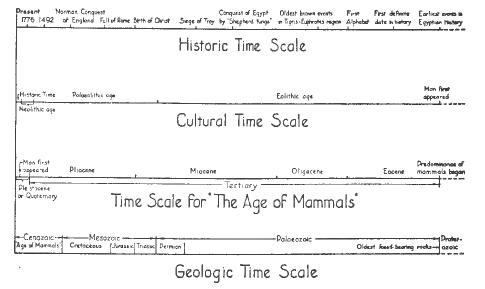
\includegraphics[width=\textwidth]{Figure_1.png}
    \caption{The comparative lengths of historic, cultural, and geologic time. Each line represents on an expanded scale the small segment at the extreme left end of the line just below it. If the geologic scale were drawn with the same number of years per inch as the historic one, it would need to be more than 20 miles long!}
    \label{fig:Lush_Figure_1}
\end{figure}

\index{Feral}Domestication implies several things, no one of which alone is sufficient to define it completely. It usually
means tameness, but individual wild animals may be tamed (as trained seals or performing bears are) without our
being willing to call them domesticated, and ranch-raised but nevertheless domesticated cattle or horses may be
very wild individuals. Domestication implies bringing the animal's growth and reproduction at least partly under
man's control, but we call pigeons and cats domesticated, even though their breeding habits and mating choices
usually are not controlled by man. Domestication implies that man converts the animal's products or services to
his own advantage or purposes, but he does this also with many wild animals, such as the fur-bearing ones. Some
of the domesticated ones, such as canaries, many breeds of dogs, and most \index{``Pet and fancy stock''}``pet and fancy stock'' serve him only
in an aesthetic way. As the word implies, domestic animals usually are kept in or near man's own dwelling places,
but usually we do not consider as domesticated the mice and rats which live in man's barns or even in his own
houses, while we do consider range-raised cattle and sheep as domestic animals although they may never have seen
a human habitation. Some of the domestic animals are dependent on man's care for their very existence, at least
in many regions. But horses, dogs, and even cattle, have at times run wild and reproduced for several generations
without any control or care by man. Strictly speaking such animals are called ``feral'' rather than truly wild.
Domestication has in most cases produced rather large changes in behavior. Some of these are conditioned by the
environmental circumstances under which the domestic animal is reared but many of them are hereditary and
presumably have been caused during the process of domestication by selection for those individuals or families
which were the gentlest, the most cooperative with man, the best trail-runners (in the case of some breeds of
dogs), etc.

In the laboratory animals, or the animals used in fish farming and in fur farming, we may perhaps be witnessing
the slow process of domestication. Some of them, like the guinea pig or the white rat, have almost as good a
claim to be called domesticated as do swine or reindeer or ducks. Others, such as mink and silver foxes, have
advanced little beyond the stage of wild animals being kept in cages as in a menagerie.

\section*{GEOLOGIC TIME}

The Cenozoic Era (the Age of Mammals) began some 50 to 75 million years ago, although the expression of geologic
time in years, particularly in the more remote periods, is very uncertain. The first mammals had come from a
reptile group called Cotylosaurs through a premammal group called Cynodonts some time in the enormous interval
between the beginning of the Permian and the end of the Triassic, but they did not become the dominant form of
animal life until the Cenozoic, being overshadowed earlier by the reptile forms. The Cenozoic is divided into
five periods, which, as far as the mammals are concerned, are chiefly noted as follows:

\textsc{Eocene}. The archaic or generalized mammals were replaced by 
modern types.

\textsc{Oligocene}. The mammals differentiated into many of the orders and families known today. An anthropoid
(Propliopithecus) is known from early in this period.

\textsc{Miocene}. This period saw the greatest variety and abundance of mammalian forms. It was a period of
extensive grasslands and restricted forest areas over much of the earth. Corresponding to that, there was a
widespread expansion and development of the grazing forms of mammals at the expense of the browsing forms. It
is probable that man's line of descent had already diverged from that of the other anthropoids by the middle
of the Miocene.

\textsc{Pliocene}. Most modern genera and even some modern species of mammals already were present at the
beginning of the Pliocene. Man's definitely human ancestors appeared during this period at a time date of
something like 600,000 to 1,000,000 years ago.

\textsc{Pleistocene}. There was periodic glaciation and with it the extinction of many of the great mammals,
such as the mammoth, the mastodon, the woolly rhinoceros, the saber-toothed tiger, and many others. Man
learned the use of tools and fire and began to domesticate animals for his own use. The period ends with the
retreat of the last great glaciation about 30,000 years ago.

\textsc{Recent} (The Age of Man). Civilization began. The historical aspects of what is known about man and his
surroundings constitute the subject matter of archaeology, and archaeology in turn gives way to history when
the written records become adequate enough to give a connected account of man's activities.
\index{Evolution|)}

\section*{CULTURAL OR ARCHAEOLOGICAL TIME}

Archaeological time is measured in stages of human culture. It does not correspond perfectly to chronological
time, since human culture did not advance contemporaneously in all parts of the world. The major subdivisions
of cultural time are as follows:

\textsc{Pre-Human Period} (the Eolithic or dawn period). This period begins with the time when man's ancestors
can first be called definitely human, something like a million years ago, and extends roughly to the coming of
pre-Neanderthal man in Europe about 200,000 years ago. The use of tools was advanced but little beyond picking
up and using such stones or clubs as happened to be handy. Probably fire was not used.

\textsc{Paleolithic Period} (the Old Stone Age). This period was marked by the use of stone and bone implements
which slowly increased in complexity and usefulness. The use of fire was learned at least by the time of
Neanderthal man. No agriculture was practiced; and there were no domesticated animals, except perhaps the dog.
The Paleolithic culture in Europe slowly developed to Neolithic culture around 25,000 years ago. What was
practically Paleolithic culture still prevailed among the aborigines of Australia and Tasmania and the Bushmen
of South Africa when the first white explorers came in contact with them.

\textsc{Neolithic Period} (the New Stone Age). This period was marked by the use of ground and polished bone and
stone weapons and tools. Neolithic man made pottery and crude textiles and basketwork. He practiced agriculture
in a crude way. He had domesticated animals of nearly all the species we have today, whereas Paleolithic man had
few or none. Neolithic man lived in huts or even in wooden houses as, for example, the Swiss Lake Dwellings. The
art of metal-working was still unknown or was practiced only on soft metals used for ornaments. The American
Indians were in a rather advanced stage of Neolithic culture when the first white explorers found them. The
cultures of the Aztecs, Mayas, and Peruvian Indians already were more advanced in many ways than the late
Neolithic cultures of Europe. They were working copper, silver, and gold, but those metals were too soft to
make useful tools. The Neolithic culture of the American Indian was behind that of Europe in the use of domestic
animals.

As long ago as 4500--4000 B.C., the city of Tepe Gawra in the Tigris valley included in its culture such things
as gold and lapis lazuli beads, temples, landscape painting, and the firing of painted pottery, although the
inhabitants had not learned to smelt copper. The earliest bit of copper known is an ornamental pin made in Egypt
perhaps as long ago as 5000 B.C. The Egyptians were working the copper mines in the Sinai peninsula regularly for
ornaments by 3500 B.C. and were using copper tools by 3000 B.C.

\textsc{Bronze Age}. The use of bronze began in Assyria by 3000 B.C. and spread west and northwest like a slow
wave. It had certainly reached the Danube basin by 2000 B.C. and perhaps Britain almost that early. Apparently
there was no bronze age in Africa, except in Egypt and on the northern coast. The other African races went
directly from the stone age into the iron age. In the bronze age in Europe, village life and complex social
customs had already developed far.

\textsc{Iron Age}. Bits of iron have been found in the Great Pyramid at Gizeh (about 2900 B.C.), but apparently
these were only rare curiosities. General use of iron for tools or weapons was begun by the Hittites in Asia
Minor about 1300 B.C. and iron supplanted bronze as the commonest metal for weapons among the Assyrians by 1000
B.C. Then its use spread rapidly.

History and archaeology are intertwined in the long period which we describe loosely as the ``dawn of history.''
The earliest definite date in history is 4236 B.C., when the Egyptian calendar began; but fragments of Egyptian
history are known from nearly 5000 B.C. Some time between 5000 and 4000 B.C. the Egyptians began to use ox-drawn
plows, and by 3500 B.C. they had an alphabet. The beginnings of history were not contemporary in different parts
of the world. For example, the definite history of Britain begins about the time of the Roman conquest; and that
of the Scandinavian countries begins about five or six hundred years later. Little is known of South Africa or
Australia before 1500 A.D. On the other hand, the history of Greece goes back some 2000 years farther than that
of Britain; Cretan history is known from nearly 3000 B.C., and a few events among the Sumerians near the Persian
Gulf can be dated at about 3500 B.C.

\section*{DATE OF DOMESTICATION OF FARM ANIMALS}

All the farm animals were domesticated long before historic times. The evidence about when and how that happened
is incomplete and consists of such things as the bones and tools found buried in the trash heaps around ancient
camp sites or caves, the drawings or carvings on the walls of caves or on ornaments. Rich sources of evidence are
the tools, weapons, utensils, and images which so many peoples placed in the graves with their dead.

Often such evidence is fragmentary and may be interpreted with equal plausibility in several different ways. Even
where evidence admits only one interpretation, the dates derived from it are necessarily minimum dates. For example,
the evidence leaves no doubt that domesticated horses were widely used in the region of the Tigris and Euphrates
rivers as long ago as 2000 B.C. and probably the first of them were brought into that region as long ago as 3000
B.C. Even if the earliest date of domesticated horses in this ``two-river land'' were established with absolute
certainty, it still remains possible that horses may have been domesticated and used a thousand years earlier at
some other place as yet unexcavated. Doubtless the thoroughly excavated sites of ancient human camps and cities
are only a small fraction of the total number which exist and may be discovered in the future.

One who reads the technical evidence and discussions can scarcely avoid the feeling that they give an unduly large
emphasis to details of the shape of horns and skull. This is natural since these parts of the animal are best
preserved and best known. It is partly justified because these parts are little affected by ordinary variations
in nutrition or other environmental influences. Yet one who surveys the considerable variability in skull and
horn shape within comparatively pure breeds today, and who considers the known cases where a single gene
substitution can cause large differences in these characteristics, must feel uneasy about placing much faith in
genealogies which rest largely on similarities or differences in the size and shape of horns or skulls. Such
genealogies are especially questionable when they are based on only a few specimens, perhaps widely separated
in time.

It is uncertain that Paleolithic man in Europe actually domesticated any animal, although he may have had the dog.
The Paleolithic aborigines who settled in Australia took the dog with them, but no other modern animal. Paleolithic
man in Europe used the horse extensively for food, but it is probable that he hunted it as game and had not really
domesticated it.

Neolithic man in Europe appears to have had nearly all of our modern domestic animals except the cat and poultry
and those animals which were found only in America or in the tropics. Some students of the evidence claim that
even in early Neolithic times the bones of the domesticated ox, swine, and sheep were already distinctly different
from their wild contemporaries. There is even considerable speculation that the domesticated races of the early
Neolithic in Europe were brought from the Caspian region or from Asia Minor in an already domesticated condition
by peoples who migrated into Europe then. A considerable amount of care was certainly given to farm animals by the
Lake Dwellers and by the men of the bronze age. It is not certain that the horse was really a domesticated animal
in Europe before the end of the Neolithic, although the men of the bronze age certainly were riding horses.

The rock-carvings from ancient Egypt and from the pre-Babylonian peoples of Sumer and Akkad, which are among the
oldest of what may be called written records, show the goat, sheep, ox, ass, pig, dog, and cat. Caring for these
animals was already a well-established part of agricultural practice, even at that remote day.

\section*{PLACE OF DOMESTICATION}

Domestication took place in the Old World except in the case of the llama, alpaca, guinea pig, and turkey, which
are native to the Americas. In the Old World, domestication seems to have taken place largely in central or
western Asia, although the evidence points to some domestication in Egypt and in Europe itself. Chickens and
elephants were domesticated in India, and at least one center of domestication for swine was in China. Domestication
may have taken place independently in several regions. This seems certainly to have happened in the case of
swine and sheep and may have happened with other animals. Much of the world, especially central Asia, is still
incompletely explored from this point of view. There were no modern mammals (except the dog and man) in Australia.
Africa south of the Sahara desert had a fauna rich in mammalian species, but none of the domesticated animals,
except the South African ostrich and the African elephant, came from there. Upper Egypt or Ethiopia was one of
the centers of domesti.cation for the ass.

\section*{SPECIES DOMESTICATED}
\index{Species|(}

For many animals it is still disputed whether they descended from a single wild species (monophyletic origin) or
from two or more wild species perhaps domesticated in different regions or at different times and later interbred
(polyphyletic origin). The main reasons for this dispute are, of course, the scantiness of the evidence and the
different biological views which the writers hold. In many cases domestication was completed so long ago that the
original wild ancestor has become extinct, or it may still be living but the domesticated form has been changed so
much that we are not now certain which contemporary wild species was the ancestor.

Polyphyletic theories are not as widely held now as formerly. The idea of organic evolution was not generally
accepted even by naturalists until well into the last half of the nineteenth century. Many of the naturalists
who wrote on the origin of domesticated animals still had in their minds traces of the old Linnean idea of the
fixity of the species. Often they had an exaggerated idea of the supposed uniformity of wild species. With this
mental background a polyphyletic origin seemed to them the only possible way to explain the tremendous diversity
of domesticated forms --- for example, the tremendous contrasts between breeds of dogs or of sheep. Modern studies
of large samples from wild populations have shown that those populations are not as uniform as many of the older
naturalists believed. Some of these modern studies have shown that enough of this variability in wild populations
is hereditary that selection, directed toward diverse goals, and other breeding practices, such as inbreeding,
could in a few generations produce distinctly contrasting races from a single wild population if man were to
control its breeding as he does that of his domesticated animals. Hence it no longer seems necessary to invoke
a polyphyletic origin as an explanation for observed diversity. The possibility remains, however, that some
domesticated animals may really have had in their ancestry crosses of distinct races or even species which were
still genetically similar enough for their crosses to be fertile. This seems to have happened in the case of
swine and sheep, although there is plenty of room for difference in opinion as to whether the races domesticated
were ever different enough and discontinuous enough to justify calling them different species. The whole question
of proper taxonomic terms for domesticated animals is in a chaotic condition. Many taxonomists hold (with
Linnaeus) that variations among races of domesticated animals are largely man-made and therefore outside the
scheme of nature which is the concern of taxonomy.
\index{Species|)}

\section*{METHOD OF DOMESTICATION}

Literally nothing is known about how domestication was first accomplished. It is only speculation to guess that
hunters first brought home a few young as pets or captured cripples from time to time and thus learned how to
care for animals. At least one Egyptian rock-picture shows hunters building a fence across the mouth of a little
steep-walled valley into which they have driven some wild animals. Wild elephants are captured in India today by
carefully planned drives. Tame elephants are then used to help chain the wild ones and to teach them to work.
Hunger is the most generally effective method of taming the most unruly among the wild ones. But it is more
difficult to tame the African elephant, even by these same methods. This suggests that temperamental aptitude
was an important element in the success or failure of early attempts at domestication.

\section*{DETAILS ABOUT DIFFERENT KINDS OF DOMESTIC ANIMALS}

\textsc{Swine}. The European wild boar (\textit{Sus scrofa}) still lives in some of the forests of Europe. It
crosses freely with domestic swine, and the offspring are fertile. Doubtless it was domesticated somewhere around
the Baltic sea in Neolithic times. A swine race or species (generally known as \textit{S. vittatus}, although
some divide it into two groups and give the name \textit{S. cristatus} to one) native to the middle and eastern
Asian mainland from western India around to central China, and found also in nearby island lands like Japan,
Formosa, Sumatra, Java and Borneo, was separately domesticated in China, perhaps as long ago as 3000 B.C. At
least one more center of domestication in Neolithic times was south or southeast of the Alps, where some of the
Mediterranean local wild races were domesticated. \textit{S. scrofa} grades into \textit{S. vittatus} by a
gradual but continuous series of local races to such an extent that modern writers (such as Kelm, 1938) are
inclined to consider them all as one highly variable species --- a \textit{``Formenkreis''}; i.e., a chain or
circle of local groups or races, each differing only a little from the ones next to it but considerably from
those farther away.

Nomadic peoples could not move swine with them easily. They generally regarded with contempt the farmers and
settled valley-dwellers who did keep swine. This may have been the origin of the Hebrew and Moslem dislike of
swine, which was later fortified by religious precept. Because nomads could do so little spreading of swine
and because wild swine by themselves do not usually migrate far, there has been in swine more than in most
species a differentiation into local races which vary from one place to another. It may be more accurate to
speak of the practice of domestication spreading from tribe to neighboring tribe rather than to speak of an
actual spread of one or of a few domesticated forms of swine.

Some of the early navigators report finding native swine on some of the islands in the southern Pacific; but
the Polynesians who settled those islands were expert navigators who had come from the general Malaysian region
only a few centuries earlier, and probably they brought swine with them. The peccaries, which belong to a
different genus, are the nearest American relatives of swine. They had not been tamed by the Indians nor, from
their behavior in captivity, does it seem likely that they can be domesticated. The breeds of swine common in
the United States probably get most of their ancestry from the European wild swine, but there may have been a
considerable amount from the Mediterranean races, and there is clear historical evidence of the introduction
of at least a little blood from Chinese swine.

\textsc{Cattle}. The family Bovidae are the most specialized of the hollow-horned ruminants. They are connected
with the other ruminants by way of antelope-like ancestors from which they diverged in the Pliocene or Miocene.
Living forms of the Bovidae include the true buffalo, the bison, musk-ox, banteng, gaur, gayal, yak, and zebu,
besides what we commonly call cattle. The musk-ox is intermediate in some respects between oxen and sheep or
goats. The musk-ox has not been domesticated, although Stefansson reports that it is well suited for
domestication. The Asiatic buffalo was in Syria in Neolithic times, but may not have been domesticated until
near Christian times. It is an important dairy and work animal of India and lands farther east and is used a
little as far west as Bulgaria. It existed in the Atlas region of northwestern Africa even after Neolithic
times. The African buffalo has never been domesticated. The banteng, gaur, and gayal are all restricted to
south-eastern Asia and the nearby islands. The banteng is the common work ox of Java, Bali, and Borneo. It is
often crossed with common cattle, but the crosses thus produced are fertile. The gayal may be only the
domesticated form of the gaur. The European bison, or wisent, and the American bison have never been really
domesticated, despite a few sporadic attempts to do so. The American bison can be crossed with common cattle,
but there is much mortality and sterility among the crossbreds. The yak is the bovine species best adapted
to cold mountain lands. It is native to the highlands of Asia north of the Himalayas and, although an
important domestic animal there, has not found practical use outside that region. Nothing very certain is
known about its date of domestication. The yak can be crossed with common cattle and with zebus and with
bison, but there seems to be some sterility among the males from such crosses.\footnote{Deakin, Alan, Muir,
G. W., and Smith, A. G. 1935. \textit{Hybridization of Domestic Cattle, Bison, and Yak}. Publication 479,
Department of Agriculture, Dominion of Canada.}

There are in the whole world between six and seven hundred million cattle which are commonly grouped under
the one species name of \textit{Bos taurus}, although some prefer to give a separate species name,
\textit{B. indicus}, to the zebu group. In the Balkans, Asia Minor, central Asia, Korea, Formosa, and in
eastern and southern Africa , there is a wide variety of forms intermediate in many respects to the extreme
zebu types and the cattle of western Europe. The more extreme types have been separate in their ancestry
for thousands of years. Carvings from the Indus valley region show bulls with extreme zebu characteristics
from as long ago as the third millenium B.C. The cattle of the United States are of purely European origin,
except some in the region bordering the Gulf of Mexico, which have considerable zebu ancestry. Concerning
the ancestry of European cattle, the most commonly mentioned species or subspecies are: (1) \textit{B. taurus}
brachyceros (or longifrons), which was in Europe as a domesticated animal early in the Neolithic and presumably
was domesticated somewhere north of the Alps or in northwestern Asia; (2) \textit{B. taurus} primigenius, the
urus or aurochs, known in Caesar's time as the wild ox of Europe\footnote{Keller says the last wild aurochs cow
in Poland was killed in 1627.} but domesticated long before (perhaps early in the Neolithic), probably south
of the Alps or in the Balkans or in Asia Minor; and (3) \textit{B. namadicus}, which was contemporary with man
in India in the early Pleistocene. Other names, common in the early writing but not seen so often now, include
\textit{B. taurus frontosus}, the Swiss spotted cattle; \textit{B. taurus brachycephalus}, the short-headed
cattle such as the Dexter, Eringer and Zillertaler breeds; and \textit{B. taurus akeratos}, the hornless
cattle of northern Europe.

\textsc{Horses}. Horses were plentiful in Europe in Paleolithic times. That they were used for food is attested
by the cracked and dismembered bones, mostly of young horses, around old camp sites like that of Solutre near
Lyons. They were probably not domesticated at that time but were hunted for food. The horse is primarily adapted
to open grassland country and apparently became rare in Europe during Neolithic times with the increasing forest
growth. Formerly it was thought that a distinct type of forest horse remained in western Europe through the
Neolithic and was the principal ancestor of the heavy or ``cold-blooded'' draft breeds. More recent studies
(Antonius, 1936) indicate that the heavy horse was developed between 1000 and 1200 A.D. in or near Friesland out
of the existing domesticated horses of Tarpan origin. Prawochenski, however, disagrees with this interpretation.
Horse bones are rare in Neolithic deposits, but bronze age deposits include bridle bits and other accoutrements
thus proving its domestication by that time.

Probably all domesticated horses of Europe and western Asia descend from the tarpan which still existed wild in
eastern Europe in the region from East Prussia southward as recently as 1700 A.D. and perhaps in the 1800's.
Some writers distinguish between a ``forest tarpan'' in the more westerly region and a ``steppe tarpan'' farther
south and east, but others think (Antonius, 1936) there was no real distinction. In eastern Asia the wild horse
of Przewalskii was reported about 50 years ago and perhaps still exists in the Mongolian desert region. It may
have been domesticated separately there. The use of the horse had reached China before historic times, but that
is of uncertain date.

The horse first appears definitely in western history before 2500 B.C. when the Neolithic Indo-Europeans from
the Caspian basin brought it into Anatolia and later to Babylonia. Presumably the Indo-Europeans from west of
the Caspian took domesticated horses westward with them north of the Black Sea at more or less the same time.
Certainly horses were in Spain and northwest Africa before any could have reached there from Egypt. The horse
first reached Egypt about 1800 B.C. when the Shepherd Kings conquered Egypt from the northeast.

The \textit{evolution} of the horse is especially well known compared with that of other mammals and is used
as a classic illustration in many books on evolution and zoology. Most of this evolution took place in the
Americas, but horses later became extinct there after some of them had migrated to Asia. There were no horses
in the Americas when the white men came. Why they died out is one of the unexplained mysteries of evolution.
Conditions were favorable for them at the time of the discovery of America by white men, as is shown by the way
the horses which escaped from the early settlers or explorers multiplied. The wild horses of the present western
ranges are descendants of these escaped horses and are often used to illustrate the difference between ``feral''
animals and truly wild ones whose ancestors never have been domesticated.

The early use of horses was for human transport and for pulling chariots in time of war. Their use for pulling
loads and for tilling the soil is a comparatively modern development.

\textsc{Asses}. The ass was in common use in Egypt and Babylonia many centuries before the horse was introduced
into those lands. Probably it was originally domesticated in Egypt or on the east coast of Africa or in southern
Arabia or around the Persian gulf. Its nearest wild relatives are found in Africa and in Asia Minor. The main
(perhaps the only) ancestor is thought to have been the Nubian wild ass, although another variety of wild ass in
Somaliland may have contributed something.

It is generally stated that the other Equidae, such as the zebra, the kiang, and the onager, have not been
domesticated. However, Antonius concludes that the ancient Sumerians had domesticated the onager and used it
extensively, even for crossing with horses to produce mules\index{Mules}. Also it is stated\footnote{The Horse Lover. 7:9.
1943.} that Burchell's zebras were formerly used on stage lines in the Transvaal.

\textsc{Sheep and Goats}. The subfamily Ovinae are all highland or mountain dwellers. Perhaps because of this
and the resulting isolation they are mightily given to breaking up into many species, subspecies, varieties,
and local races. There is no single trait which distinguishes all goats from all sheep, although there are some
things which are characteristic of most sheep and few goats or vice versa. Besides the true sheep and the true
goats, there are, according to Antonius, the following groups of Ovinae: (1) The Hemitragus group of primitive
or short-horned goats with four teats. Three living species are found in the mountains of India and southern
Arabia. (2) The ibexes or steinbocks, which resemble the true goats rather closely and are fertile with them
but have contributed nothing to their ancestry. They are all mountain dwellers, and Antonius lists seven species
in the mountains from the Himalayas to the Pyrenees and another from the mountains of southern Abyssinia. (3)
The burrhel or blue sheep of Tibet. (4) The maned sheep or aoudad, now restricted to the Atlas mountains but
extending as far east as Egypt even in historic times. (5) The argali group, which are rather sheep-like and
include an enormous number of local races besides the argali itself and Marco Polo's sheep. The argali group
probably did not contribute anything to the ancestry of domesticated sheep, unless perhaps something to the
fat-rumped races. This is disputed by some investigators (Gromova, 1936) who believe the argali group was
important in the ancestry of domesticated sheep. (6) The thick-horned sheep, of which there are an enormous
number of local races extending from the northern Himalayas northeastward over Kamchatka and Alaska to
California. The Big Horn Sheep of the Rocky Mountain region is an example. Probably this group played no
part in the ancestry of domestic sheep. There have been a few accounts of crosses between domestic sheep
and Big Horn Sheep in western United States.\footnote{Jour. Wildlife Management 9:82-83. 1945.}

Domesticated goats are believed to descend mostly from \textit{Capra prisca}, which is known from Pleistocene
fossils from Greece northward, or from \textit{C. aegagrus}, the Bezoar goat or Psaang, which still exists
through the mountainous regions of Asia Minor and Persia and in the past has extended from Sind to as far west
as Crete. Also mentioned among the true goats are \textit{C. dorcas} (which some think only a form of
\textit{C. prisca}) from the Jura mountains, and \textit{C. falconeri}, which is extraordinarily given to
the development of distinct local races and lives in the region around Afghanistan. Some of the tame Egyptian
goats resemble \textit{C. falconeri} rather closely, but it is not certain that they descend from it in any
part. Nothing is known about the place of domestication of the goat, nor about the date of domestication,
except that it must have been very remote.

Domestic sheep are thought to descend mainly from the mouflon, \textit{Ovis musimon}, which is still found
wild in Sardinia and Corsica and interbreeds freely with domesticated sheep, and from \textit{O. vignei},
the urial, which is found from Turkestan to Asia Minor. Some writers think that a part of the ancestry of domesticated 
sheep came from \textit{O. orientalis}, the mouflon of Asia Minor and Armenia, or from \textit{0. arkal}, which is
found east of the Caspian Sea. There is more confusion and disagreement about the ancestry and classification of sheep 
than of any other farm animal.

Domestication of the sheep took place so long ago that taxonomic names have even been given to the forms found in 
deposits from various stages of human culture. Thus, there is talk of a ``turbary sheep, 
\textit{Ovis aries palustris}'' and of a ``copper-age sheep, \textit{Ovis aries studeri}.'' Early Neolithic man in Europe 
certainly had domesticated sheep with him, but where or when he got them can only be conjectured from what is known
about their geographical distribution. There is an enormous variety of breeds and races of domesticated sheep. The 
classifications proposed for convenience in referring to these are generally based on the nature of their wool and the 
length and fatness of their tails. Antonius classifies them for that purpose as follows:
\begin{enumerate}
	\item[1.] Long-tailed sheep
	\begin{enumerate}
		\item[A.] The wool sheep of Europe. These include all the breeds which are prominent in the United States.
		\item[B.] Hairy sheep originally prevalent all over Africa. The black-headed Persian sheep of South Africa is an example.
	\end{enumerate}
	\item[2.] Fat-tailed sheep, usually with a long tail, fat at the upper end but slender at the tip. Karakuls are an example.
	\item[3.] Short-tailed sheep, such as the Heidschnucke of Germany and other marsh or moorland sheep of northern Europe. 
	\item[4.] Fat-rumped sheep, which were originally native to high Asia east of where the fat-tailed sheep developed.
\end{enumerate}

\textsc{Dog}. Zoologically the dog is essentially the same as the common wolf of the northern hemisphere.\footnote{Crosses
between dogs and wolves are frequent (Jour. of Genetics 43:359--414. 1941).} The dog was the only 
domesticated animal found in both the New and the Old Worlds. The polyphyletic origin of the dog, involving the jackal
as well as the wolf, was once widely believed, but that belief has almost disappeared now. The dog may very well have 
been the first animal domesticated. Chaldean and Egyptian monuments show several distinct breeds in existence four or 
five thousand years ago. The Incas in Peru had bulldogs as well as their ordinary breed (Hilzheimer, 1936).

\textsc{Cat}. The Egyptians domesticated the African wild cat. Thence it was probably introduced to Italy by Phoenician 
traders some centuries before the Christian era. A European wild cat and perhaps also a Chinese wild cat may have 
contributed to the ancestry of modern domestic cats. 

\textsc{Camel}. The single-humped camel, \textit{Camelus dromedaritts}, was domesticated probably in Arabia or 
northeastern Africa, perhaps near the very beginning of Egyptian civilization or perhaps not until near 1000 B.C.
The two-humped camel, \textit{C. bactrianus}, was domesticated in Asia somewhere between Iran and the Gobi desert.
It had reached Syria at least by 1000 B.C. and perhaps a thousand years earlier. It is now the common camel in China
and the regions just northwest, although the other occurs also. 

The llama and alpaca are the only living American representatives of the camel family, although that family went
through most of its evolution in North America. They were domesticated by the ancient Peruvians from the wild
guanaco, \textit{Lama huanachus}, long before the Spanish conquest. The wild vicuna, \textit{L. vicugna}, is a close
relative. In the Incan agriculture the alpaca occupied somewhat the place of the sheep in ours, but the llama was used 
extensively as a beast of burden, as well as for its meat and wool. Llamas sometimes are used for dairy purposes, too. 

\textsc{Reindeer}. \textit{Rangifer tarandus} is the Scandinavian wild form which was domesticated by the Lapps
and later introduced to Alaska and arctic Canada. \textit{R. caribou}, the caribou of Canada, has not been
domesticated. One report has it that reindeer were domesticated in the Yenisei River basin about the time of Christ. 

\textsc{Elephants}. Elephants were domesticated at least as long ago as in ancient Carthage. Presumably they were
used in India much earlier. Alexander used them in his battle with Darius in 331
B.C.\footnote{See Armandi's ``Histoire militair e des elephants.'' Paris. 1843.} in Mesopotamia. 

\textsc{Chickens}. Chickens came from southeastern Asia and are generally believed to have descended from
\textit{Gallus bankiva}, the jungle fowl of India. It is not certain that more than one species was involved. 
Domesticated chickens were kept in China at least as early as 1400 B.C., and from India had arrived in Babylon by 600
B.C., in Greece by 500 B.C., and in Rome well before the Christian era. The actual introductions may have been
centuries earlier. 

\textsc{Geese}. These came from the grey laggose, \textit{Anser anser}, and perhaps also the Chinese goose,
\textit{Cygnopsis cygnoides}. The date is uncertain, but geese were kept by the ancient Romans several centuries
before the Christian era, as witness the legend about the cackling of the geese which on one occasion saved Rome
from invaders. There may have been several independent domestications.

\textsc{Ducks}. Probably these all come from the mallard duck, \textit{Anas boschas}, although there are many other 
species of wild ducks. Ducks probably were not domesticated before Roman times. 

\textsc{Guinea}. The guinea comes from the Guinea coast of western Africa. The wild species is
\textit{Numida meleagris}. The guinea was known to the Romans as a domestic fowl but later ceased to be kept in
Europe and was reintroduced by the Portugese in the sixteenth century.
 
\textsc{Peacock}.\textit{Pavo cristatus} is found in India and Ceylon. \textit{P. muticus} is found in Burma and
Java. Either or both may have contributed to the origin of domestic races. The peacock was a relatively late arrival
in European agriculture. It was first domesticated in Persia, or at least first knowledge of it came to Europe from 
Persia. 

\textsc{Turkey}. The peoples of ancient Mexico and Peru had domesticated the turkey long before the discovery of
America by white men. The wild Mexican turkey, \textit{Meleagris mexicana}, is thought to have furnished 
most of the ancestry, but \textit{M. gallopavo} from the Atlantic coast of the United States and \textit{M. ocellata} 
from Central America are sometimes mentioned in that connection. 

\textsc{Fur-Bearing Animals}. Such animals as the \textit{fox}, \textit{mink}, \textit{marten}, \textit{ferret},
\textit{skunk}, \textit{muskrat}, etc., are extensively reared in captivity but probably should not yet be called
truly domesticated. They may represent stages in domestication through which our farm animals passed far back in
Neolithic times.

\textsc{Laboratory Animals}. Among the laboratory animals, the \textit{guinea pig} probably should be called
domesticated. South American Indians were breeding it in captivity for food before the white man came. The
\textit{white rat} is an albinotic strain  of the common Norway rat, \textit{Mus norvegicus}. Probably the albino rat
was domesticated before the beginning of the nineteenth century. An albino rat colony in England in 1822 is reported. 
Fancy races of \textit{mice} were known in ancient Troy perhaps as long ago as 1200 B.C. and probably in China as far
back as 1100 B.C., since a Chinese dictionary of that date had a special word for the spotted mouse. Domestic
\textit{rabbits} are descended from the European rabbit, \textit{Oryctolagus cuniculus}. It was probably domesticated
in the Spanish peninsula or southern France, perhaps as early as 1000 A.D. 

\textsc{Bees}. Honeybees are mentioned frequently in the Old Testament and in early Roman writings on agriculture.
They were brought to America from Europe. Bumblebees were already in America when the first white explorers came.

\textsc{Silkworm Culture} developed in China, possibly longer ago than 2000 B.C. It did not spread to other countries
until the Christian era. 

\section*{REFERENCES}
Encyclopedias, especially the \textit{New Brittanica} and the \textit{Americana} and Volume 3 of Bailey's
\textit{Cyclopedia of American Agriculture}, furnish a good starting point for general information. Consult several
in order to note the disagreement as to fact and the confusion about specific classification.

The \textit{National Geographic Magazine} occasionally has an article on some domestic animal with pictures and 
descriptions of many of the living breeds or races. Some of the recent ones are as follows: 
\\
\begin{hangparas}{0.25in}{1}%
November, 1923. The story of the horse. W. H. Carter. 44:455-66.

December, 1925. The Taurine World. A. H. Sanders. 48:591-710.

April, 1927. The races of domestic fowl. M.A. Juli. 51:379-452.

March, 1930. Fowls of forest and stream tamed by man. M.A. Juli. 57:327-71.

April, 1935. Man's winged ally, the busy honeybee. James I. Hambleton. 67:401-28.
\end{hangparas}

Many of the original articles which treat of domestication in detail are in the German language, being written by 
Germans, Austrians, or Swiss. Among the more recent of these, should be mentioned:

\begin{hangparas}{0.5in}{1}%
(Various authors). 1936. Neue Forschungen in Tierzucht und Abstammungslehre. Bern: Verbandsdruckerei 
A.G. (contains the articles by Gromova and by Hilzheimer).

Antonius, Otto. 1922. Grundz\"{u}ge einer Stammesgeschichte der Haustiere. 336 pp. Jena: G. Fisher.

---. 1936. Zur Abstammung des Hauspferdes. Zeit f. Z\"{u}cht. B. 34:359-98.

Kelm, Hans. 1938. Das postembryonale Schadelentwicklung des Wild- und Berkshire-Schweins. Zeit. f. Anal. u. Entwicklungsgeschichte 108:499-559.

Klatt, B. 1928. Entstehung des Haustiere. Berlin: Gehr\"{u}der Borntraeger. 
\end{hangparas}

In the English language the following original articles or books treat of domestication in some detail:

\begin{hangparas}{0.5in}{1}%
Allen, R. L. 1847. Domestic animals. 227 pp. New York: Orange Judd \& Company.

Amschler, Wolfgang. 1935. The oldest pedigree chart. The Jour. of Heredity, 26:233-38.

Brown, Edward. 1906. Races of domestic poultry. 234 pp. London: Edward Arnold.

Ewart, J. Cossar. 1926. The origin of cattle. Proc. of the Scottish Cattle Breeding Conference for 1925, pp. 1-16.

Holmes-Pegler, H. S. 1929. The book of the goat. 255 pp. London: The Bazaar, Exchange and Mart.

Jennings, Robert. 1864. Sheep, swine, and poultry. Philadelphia: John E. Potter \& Company.

Lydekker, Richard. 1912. The horse and its relatives. 286 pp. London: G. Allen \& Company.

---. 1912. The ox and its kindred. 271 pp. London: Methuen \& Company.

---. 1913. The sheep and its cousins. 315 pp. New York: E. P. Dutton \& Company.

Morse, E. W. 1910. The ancestry of domesticated cattle. pp. 187-239 in the Twenty-seventh Annual Report of the Bureau of Animal Industry, United States Department of Agriculture.

Ridgeway, William. 1905. The origin and influence of the Thoroughbred horse. 538 pp. Cambridge University Press.

Shaler, N. S. 1895. Domesticated animals. 267 pp. New York: Charles Scribner's Sons.

Among French books, the following is unique enough to warrant special mention:

Chollet, et al. (since 1903) Les Animaux. 550 pp. Paris: Bong et Cie.
\end{hangparas}

Among the general references, dealing briefly with man's cultural stages while he was domesticating the 
animals or with evolutionary aspects of the subject, may be mentioned:

\begin{hangparas}{0.5in}{1}%
Breasted, J. H. 1938. The conquest of civilization. 669 pp. New York: Harper Brothers.

Matthews, W. D., and Chubb , S. H. 1921. Evolution of the horse. No. 36 of the Guide Leaflet Series, American Museum of 
Natural History, New York City.

Newman, H. H., et al. 1927. The nature of the world and of man. (pp. 332-80 for the story of man and civilization.) 
University of Chicago Press.

Sumner, F. B. 1932. Genetic, distributional and evolutionary studies of the sub-species of deer mice (Peromyscus). Bibliographia Genetica, 9:1-106.
\end{hangparas}
\chapter{Consequences of Domestication}
\label{cha:consequences-of-domestication}

The fundamental laws of heredity and the mechanics and physiology of reproduction are the same among domesticated animals as 
among their wild relatives. The change from the wild to the domesticated condition did not alter these laws nor create any 
new inheritance. The changes which domestication did bring about were an increased amount of inbreeding and outbreeding and 
assortive mating and the addition of artificial selection to the forces of natural selection. The changes in environment 
which accompanied domestication doubtless permitted many differences in heredity to show themselves more clearly than they 
could in the environment of wild animals, and thus to be more readily and accurately selected. For example, when feed is so 
scarce that no animal gets all it wants, hereditary differences in ability to fatten could hardly show themselves as clearly 
as they can in a well-managed feedlot. But there is no direct evidence to indicate that the changed environment directly 
\textit{created} any new genes or hereditary differences.

\index{Inbreeding|(}\textit{Increased inbreeding} happened because domesticated animals were more narrowly restricted (by tethering, herding, or 
fencing) to growing up, remaining, and reproducing in the same region in which they were born. Soon the animals around one 
community or village would all become related to each other. Most breeders, even among primitive peoples, intentionally 
avoided the very closest inbreeding; but often the pedigrees were known only for a generation or two, or only in the female 
line. Under such circumstances, attempts to avoid inbreeding merely made the inbreeding less intense so that more time was 
required to produce the same amount of fixation and uniformity in the stock. That gave more opportunity for the accompanying 
selection to discard undesired results of the inbreeding than if the inbreeding had been extremely close. Even when 
obstacles to exchange between tribes were greatest, some introduction of outside blood went on either by trade or by war. 
Doubtless these exchanges usually involved stock from only the closest neighboring tribes. Such animals, as a result of 
previous exchanges, would already be more closely related to those among which they were introduced than animals which might 
have been chosen at random from the whole species. There would have had to be a large amount of such interchange to prevent 
this inbreeding from bringing about a situation where almost every tribe or community would have its own type of each kind 
of animal. Doubtless the intensity of this inbreeding varied greatly from region to region according to the nomadic habits 
of the people, geographic barriers, or social customs which may have prevented extensive trade with neighboring tribes, and 
the extent to which their beliefs about breeding led them to try deliberately to prevent this inbreeding by taking special 
pains to get sires from unrelated or remotely related stocks. This extra inbreeding resulting from restricting the 
movements, and also from limiting the number of breeding males, may well have been one of the most potent forces leading to 
the production of diverse races among domestic animals. It does not seem possible now to measure its past importance 
accurately, since so little is known about actual breeding customs until very modern times. The geographic or physiologic 
isolation, which in nature divides so many species into small sub-groups between which crosses occur only at rare intervals, 
is the very same kind of a process in principle, but probably is rarely as extreme in nature as it is under domestication 
where man has added so many artificial barriers to the natural ones.

\index{Outbreeding|(}\textit{Increased outbreeding} has certainly resulted now and then from domestication. By the agency of man, breeding 
animals could be transported far beyond the area in which they were born or over which they could have wandered before they 
were domesticated. Thus they could be crossed on races more diverse than they would have encountered if they had remained in 
the wild state. Knights returning from the Crusades brought with them stallions from Arabia. Cattle were brought from 
Holland to England across water which would have been impassable to wild cattle. In a later day Merino sheep were taken from 
Spain to many lands, Angora goats came from Turkey to the United States and to South Africa, zebu cattle came from India to 
Brazil and to the Gulf Coast of the United States, and Shorthorn cattle went from England to the Argentine and Australia. 
Many other examples could be cited to show how this process went on in historic times. The diverse races of swine from which 
the Poland-China breed was formed could hardly by any conceivable circumstances have come together anywhere on earth without 
the intervention of man to transport them. 

Presumably this process has gone on more rapidly in the last three or four centuries of exploration and widespread trade
than it did formerly, but Phoenician traders were traveling the length of the Mediterranean and skirting the western shores 
of Europe as far as Britain nearly three thousand years ago and doubtless helped exchange some of the smaller animals at 
least. Invading armies or migrating peoples usually carried with them much livestock from their native lands; some of these 
were mingled with the breeding stock of the countries through which they passed. Two thousand years ago Hannibal and 
Hasdrubal took their armies and livestock, including such large and unwieldy animals as elephants, from Carthage along the 
northern coast of Africa to Spain and over such mountains as the Pyrenees and Alps almost to Rome itself. Also, Alexander 
the Great took large numbers of livestock with his armies on the road from Greece to India and had with him men who made 
careful notes about the strange livestock they saw in the new lands. In the early thirteenth century the armies of Genghis 
Khan and his sons, with their enormous reserves of cavalry horses, ranged all the way from eastern China to central Europe. 
The passing of that band of horses (with the inevitably large amount of straying and robbing) must have changed greatly the 
genetic composition of the local races in the regions through which they passed. With such cases known from definite 
history, it is only reasonable to suppose that similar exchanges by migrations or wars had been taking place almost since 
the beginnings of domestication. Here again, as in the case of geographic isolation, there must have been much more of such 
exchanges in some parts of the world than in others. 

A combination of moderate inbreeding alternating with occasional wide outbreeding is an effective plan for producing many 
distinct families which are moderately uniform within themselves. A population being thus bred is in a more favorable 
condition for selection to be effective than if matings within the group selected to be parents were entirely at random. In 
this way domestication made conditions more favorable for the formation of distinct races than exist among wild animals. 
\index{Inbreeding|)}
\index{Outbreeding|)}

\index{Selection|(}
\textit{Selection} means differences in reproductive rates within a population, whereby animals with some characteristics 
tend to have more offspring than animals without those characteristics. Thereby the genes of the favored animals tend to 
become more abundant in the population and those of the less favored animals less abundant. Artificial selection differs 
from natural selection only in the kind or degree of the characteristics which are thus favored. Also, in many cases 
artificial selection may be more intense, less of the decision being left to chance or to accidental circumstances than in 
the case of natural selection.

Natural selection did not wholly cease with domestication. More of the weak and sickly than of the strong and vigorous are 
still doomed to die before they reach breeding age. This will happen whether the breeder consciously aids in this selection 
or not. Indeed, some of it will happen in spite of the breeder's efforts if he tries to breed a type which is rather frail 
or susceptible to disease. Among domesticated animals natural selection is merely supplemented by man's selections. In 
making his decisions as to which animals should leave few and which should leave many offspring, man often strongly 
emphasizes characteristics which were of little worth in a state of nature. Other qualities valuable in the wild state 
became useless or nearly so when man began to protect his animals against their enemies, against cold and against 
starvation. Thus, man's selection may differ from natural selection both in \textit{intensity} and in \textit{direction}.

The practice of favoring for breeding purposes those animals which in their owner's opinion were the most desirable ones 
must have begun with domestication itself. The recognition that offspring tend to resemble their parents and other near 
relatives occurred at so early a cultural stage that proverbs embodying this idea are found in practically all languages, 
even those of extremely primitive people. Primitive man was doubtless quite shrewd enough to put this knowledge into 
practice on his domesticated animals. Castration is one of the most ancient of surgical practices. Medical literature 
traces it back at least as far as 700 \textsc{B.C.}, and in the Bible there is frequent reference to eunuchs in the time of 
Solomon or earlier. Eunuchs are mentioned in the Code of Hamurabi; ca. 2000 \textsc{B.C.} Castrated bullocks (balivarda), 
as distinct from bulls, are mentioned in the Puranas of the Hindus, which deal with the events of the Aryan migrations into 
northwestern India probably as long ago as 2400-1500 \textsc{B.C.} (Since the Puranas were not put into writing until much 
later, the words may have been changed during the interval). The general practice of castration must have intensified the 
selection which was practiced among males.

The Roman agricultural literature of about two thousands years ago\footnote{Harrison, Fairfax. 1917. \textit{Roman Farm 
Management}. 365 pp. New York: The Macmillan Company.} contains many bits of advice about the kinds of animals to select 
for different purposes. Much of this they had copied from still older writings, such as those of Mago the Carthaginian. It 
is certain that artificial selection has been practiced by man for thousands of years, although there seems to be no way of 
measuring the intensity with which it was practiced.

Another aspect of selection which was intensified by domestication was that the characteristics favored for one set of 
conditions might not be the same as those favored under other conditions. This, of course, was true in nature also, 
contrasting characteristics sometimes being favored for life on the open grasslands or for life in the forest, for 
mountain or lowland, for tropics or temperate climates, etc. In nature these would often --- perhaps usually --- be 
characteristic of wide areas with broad transitional zones between them. Under domestication one man might prefer a certain 
type of horse or cattle, and his next-door neighbor or the people of the very next village might prefer and select for a 
distinctly different type. Indeed, as agriculture became more complex the same man might keep two or more types of the same 
species, each being preferred for some special purpose. For instance, the ancient Egyptians had several breeds of dogs, and 
modern farmers keep different breeds of cattle for beef and for dairy purposes. So far as one breed or type is concerned, 
this is nothing but selection directed toward that particular ideal; but, from the standpoint of the whole species, this is 
assortive mating, which is a powerful tool for producing diversity within a species. This seems certain to have been more 
intensified under domestication than it was in nature.
\index{Selection|)}

\section*{SUMMARY}

Domestication merely intensified forces or processes which already existed in nature. Increased inbreeding alternating with 
wider outcrossing, more intense selection devoted toward a wider variety of goals, and mating like to like wherever one 
man or tribe was breeding the same species for two or more different goals, all had the net effect of tremendously speeding 
up the slow process of evolution as it occurs in nature, until remarkably large changes were made in animals under 
domestication during what was a very short period in terms of geologic time. That the changes thus brought about were at 
the maximum rate possible seems highly unlikely. If further changes are desired, it is probable that the possibilities in 
most directions are by no means exhausted and that intelligent use of these same processes can result in much faster 
progress than has been averaged during the long (in terms of human lifetimes) history of domestication.
\index{Domestication|)}
\chapter[Beginnings of Pedigree Breeding and Registry Societies]{The Beginnings of Pedigree Breeding and the Formation of Breed Registry Societies}
\label{cha:breed-registry-societies}
\index{Origin of breeds|(}
\index{Pedigree breeding, beginnings of|(}

\begin{quote}
``The virtues of their fathers live on in bulls and in stallions.'' --- Horace
\end{quote}

\begin{quote}
``Who would grow spirited stallions for the Olympic prizes or strong bulls for the plow, let him choose carefully 
the females who will be their dams.'' --- Virgil
\end{quote}

Emphasis on ancestry in human genealogies is older than history, although human pedigrees may have been used more for 
social purposes, such as to determine the inheritance of property or of rank in a caste system of society, than because of 
definite beliefs about the inheritance of physical and mental qualities. Often these pedigrees recorded only the male or 
only the female line of descent. The genealogies in the early chapters of Genesis are examples of this. 

Pure breeding is also an ancient idea as applied to man, not only in those peoples which had a pronounced caste system of 
society but also in many others where a tribe was warring on neighboring tribes, or a conquering race was trying to live 
with but keep itself ``pure'' from a conquered or slave race. Also, many tribes or races with a simpler social structure 
cherished myths about their racial origins which implied that they alone were the chosen people descended from the sun or 
the moon or some other deity, while other peoples were of inferior or mixed descent. In most (but not all) human societies 
there has been a heavy social prejudice against the ``half-breed,'' which in general has meant that the half-breed and its 
descendants must come up to higher standards of individual excellence than the average ``purebred'' before they would have 
an equal chance to contribute to the inheritance of the future race. 

The Arabs in their horse breeding more than a thousand years ago were memorizing the genealogies of their horses, but we 
have no detailed knowledge of how these genealogies were used --- if at all --- to guide them in making the matings.\index{Origin of breeds} 
Probably, like the modern Arabs, they traced the pedigrees only in the female line and used the family name only as an aid 
to selection,\footnote{Nurettin, Aral, and Selahattin, E. 1935. \textit{Der heutige Stand der Pferdezucht in 
Arabien.} Zeit. f. Z\"{u}chtung. (Reihe B), 33:13-38.} also taking some care to avoid close inbreeding. The Romans of the 
time of Varro and Cato made many comments about the kinds and types of animals which should be selected for breeding 
purposes but apparently made no attempt to memorize or record long pedigrees for their livestock. Varro's comments on the 
importance of judging the breeding worth of a sire by the quality of his get show that in a general way they were aware of 
the importance of the progeny test and the use of pedigrees, traced at least to the parents and grandparents, to help them 
to a more correct estimate of an animal's breeding worth.

``Throughout the Middle Ages the authority of the written word almost completely displaced firsthand observation and 
experiment in the search for truth.''\footnote{Mees, C. E. Kenneth. 1934. Scientific Thought and Social Reconstruction. 
\textit{Sigma Xi Quarterly}, 22(No. 1):17.} Largely because of this, knowledge of the mechanics and laws of heredity 
advanced but little. Most of the learning was preserved in the monasteries and what little is known about agriculture in 
the middle ages comes mostly from the account books, inventories, and fragmentary notes kept in connection with the farming 
operations of the monasteries. It was not until 1700 that enough was written and preserved to give us a connected account 
of agricultural practices.

The use of pedigrees in the modern manner began in rural England late in the eighteenth century, and the general formation 
of breed registry societies\index{Origin of breeds} began around the middle of the nineteenth century. Robert Bakewell is generally given credit 
for setting the pattern of modern animal breeding and is sometimes called the founder of animal breeding. Perhaps this is 
giving too much credit to one man, but at any rate pedigree breeding was established in his time, and his own outstanding 
success had more to do with making it popular than the efforts of any other one man did.

\index{Bakewell, Robert|(}Robert Bakewell was an English farmer or country gentleman who lived from 1725 to 1795.\footnote{A more complete account of 
Bakewell's work and of the conditions of animal breeding then is given on pages 176-189 of Lord Ernie's \textit{English 
Farming, Past and Present}. 1936.} We first hear of his agricultural efforts when he began to manage the estate at Dishley 
in 1760. He wrote little or nothing about himself. He was a good farmer in other things besides his stock breeding, having 
taken a prominent part in the introduction of turnips and other root crops into English agriculture. He was a good 
observer, a keen student of anatomy and probably a good judge of livestock. According to some accounts he even kept for 
future reference specimens of the bones or pickled joints of animals which he had bred and which he regarded as nearly 
ideal. He told so little about his operations that many of his contemporaries thought there was something mysterious about 
them. Some writers hint that this was done deliberately to avoid competition or censure. This latter point is made because 
an important element in his procedure was the deliberate and intense use of inbreeding. At that time there was even more 
prejudice against inbreeding than there is today, and many people thought it almost sacrilegious. Perhaps Bakewell thought 
it no use to invite criticism by proclaiming openly what he was doing. There is also more than a hint that he kept his 
operations secret because of certain extreme outbreeding he was practicing which, if known, might have injured the 
commercial reputation of his stock. Thus, there were rumors of a mysterious black ram used in his sheep breeding which 
visitors were never permitted to see and whose existence he would never admit.

Bakewell's own breeding work was with the old Longhorn cattle, Leicester sheep and Shire horses. He was so successful with 
these that his animals came into great demand as breeding stock. He inaugurated the practice of ram-letting. That is, he  
did not sell his best males out-right, but rented the use of them a year at a time. His annual auctions, or ram-lettings, 
attracted great attention and were a distinct financial success. He is said to have received as much as 1,200 guineas for 
one year's use of a ram. By this practice of ram-letting, the best sires came back to him each year and any whose progeny 
had proved them much better than the others could be kept for use in his own flocks or herds. There seems to be no record 
of how many times he took back for his own use a sire which originally he had thought not quite good enough for that, but 
no doubt such instances occurred. 

Bakewell's success attracted many imitators. From many parts of England ambitious stockmen went to Dishley to work with 
Bakewell and study his methods. Some of them stayed for as much as six months. Returning home they applied his methods to 
stock secured from him or to what they thought were the best of their own local animals. The details about these students 
and what they did are poorly known, but it is certain that the Collings who laid the foundations of the Shorthorn breed 
were in close touch with Bakewell and that men from Herefordshire were students with him. Enough of Bakewell's followers 
won distinct success that here and there all over England there soon began to be groups of animals closely related to each 
other and similar in type.These were the groups from which came the modern breeds, most of which were not formally 
organized as such until later. 

The \textit{principles} which Bakewell used included such things as: ``Like produces like or the likeness of some ancestor; 
\index{Inbreeding|(}inbreeding produces prepotency and refinement; breed the best to the best.'' His greatest contribution to breeding methods 
lay in his appreciation of the fact that produces like or the likeness of some ancestor; 
inbreeding was the most effective tool for producing refinement and fixing type. 
He was reluctant to make any \index{Outcross}\index{Outbreeding}outcrosses at all when his own stock seemed to him better than that of his neighbors. With his 
willingness to inbreed was coupled a good knowledge of anatomy and a keen interest in the subject of what types of animals 
were best suited to his agriculture and should be set up as goals. 
\index{Bakewell, Robert|)}

The economic setting of the times, of course, had much to do with the increased interest in breeding improved animals. The 
enclosures of the ``common lands'' had given the individual farmer opportunity to breed his own stock as he pleased and to 
reap the rewards of anything he might do to improve them or to build up the fertility of his own lands. The introduction of 
clovers and root crops to English agriculture had made more intensive animal husbandry possible and had supplied a store of 
roughages suitable for winter feeding. The times were ripe for commercial appreciation of animals which could utilize the 
crops of the new agriculture better than their contemporaries and which would produce a quality of product well suited to 
contemporary market demands. The warfare through the latter half of the eighteenth century, finally coming to a climax in 
the Napoleonic wars, often made prices high for farm products. Afterward, the industrial revolution and the steadily 
expanding urban population of Britain made a rising market for agricultural products, more particularly for those like meat 
which, in the days before refrigeration, could not be imported in the fresh state from the New World. When the improvement 
which Bakewell and his followers had made in their breeding stock began to be known in other lands, the export of breeding 
stock to those lands became a considerable source of income to British stockmen. Appreciation of the importance of this was 
a spur to further improvement in order to keep the foreign customers coming back for fresh breeding stock and had much to do 
with guiding the policies of breed registry societies.\index{Origin of breeds}
\index{Inbreeding|)}

\section*{BREED REGISTRY SOCIETIES}
\index{Breed associations|(}

As long as each breed was local the private records of each breeder were adequate for his own purposes. He usually knew at 
least the sires used by his fellow breeders and knew the integrity of those breeders well enough to have some idea of how 
much he could depend on their statements or records when purchasing breeding animals from them. But in time the number of 
breeders increased until many of them were utter strangers to each other, and the number of animal generations in the 
pedigrees increased until no man could remember all of the foundation animals far back in the pedigrees. To supply this 
knowledge and to prevent (as far as other breeders could) unscrupulous traders from exporting grades or common stock as 
purebreds, herdbooks were formed. The latter motive was very important\footnote{For example, many events in Bates' book
(1871) illustrate the incentive which the American demand for Shorthorns gave to the formation of the Coates herdbook.} 
and generally the herdbook was established soon after there began to be a considerable export demand.

\index{Herdbooks|(}
The first herdbook was ``An Introduction to the General Stud Book'' for the Thoroughbred horse and appeared in 1791. In it 
were recorded the pedigrees of the horses winning important races. It was aimed, therefore, at recording the pedigrees of 
performers rather than of all members of the pure breed. The Shorthorn herdbook, which first appeared in 1822, was the next 
one formed and may be taken as an example of the modern type of herdbook which aims at including the pedigrees of all 
animals of the pure breed. The Shorthorn herdbook, however, like the one for the Thoroughbred horse, would accept for entry 
outstanding individuals or performers which would be called high grades in the United States. Later herdbooks were largely 
modeled after the more successful of the early ones. An English Hereford herdbook was published in 1846 and a Polled Herd 
Book (for Aberdeen-Angus) in 1862. The first swine herdbook in the world was that of the American Berkshire Association, 
which appeared in 1876. The Berkshire Society in England was established first in 1883. The first herdbooks in the 
continental countries of Europe appeared at a later date than in Britain. Studbooks for horses were founded in France in 
1826, in Germany in 1827, and in Austria in 1847. The first cattle herdbook in France was established in 1855, the first 
German one in 1864, the first Dutch one in 1874 and the first Danish one in 1881. 

The Shorthorn herdbook was undertaken as a private venture by George Coates, who had been a Shorthorn breeder in a small 
way. A number of the Shorthorn breeders helped finance him and each was to receive a copy of the book. The other copies 
were to be his personal property to sell for whatever profit he could. He was already acquainted with many breeders, and 
from each of them he secured such information as he could about the animals which that man regarded as genuine Shorthorns. 
No doubt there was plenty of dispute about that. That is, some breeders would say that certain animals should be included 
in the records while others would think that those animals were not sufficiently desirable to be included as genuine 
Shorthorns. Coates was criticized, of course, for many of these decisions; and it was even charged\footnote{\textit{See} p. 
38 in Bates' \textit{History of Improved Shorthorn or Durham Cattle.}} (perhaps unjustly) that his favoritism to his 
personal friends went to the extent of printing for their cattle false pedigrees which would make them sell well to the 
American trade, then becoming important. Where Coates included animals which the majority of the breeders thought were not 
really pure, the breeders themselves could remedy the situation by having nothing to do with those animals or their 
descendants -- a course of action which is still open today and which is still used freely wherever falsification of 
pedigrees is suspected but evidence is not complete enough to justify canceling the registration. Wherever Coates omitted 
from the first volume of his herdbooks animals which the majority of breeders thought should have been included, such 
mistakes could be corrected by including these pedigrees in succeeding volumes of the herdbook -- a process no longer 
available wherever herdbooks are entirely closed to all but the offspring of registered parents.

Some of the very early breeders objected to furnishing pedigrees of the animals they sold, believing that they would thus 
give away valuable trade secrets. The demand for full information about pedigrees, however, finally prevailed over the
``trade-secret'' idea; and it became accepted as a matter of course that anyone selling breeding stock should furnish full 
identification of their immediate ancestors.

Doubtless many of the contemporary breeders felt that this herdbook of Coates was only a hobby of his which would disappear 
with his death; but, as the breed became more popular and the number of breeders increased and the number of generations to 
be remembered in the pedigrees grew larger, the difficulties which first prompted Coates to the formation of the herdbook 
became greater. Eventually every breeder admitted the necessity of the herdbook, in view of the customer demand for 
pedigrees, and depended upon it in his purchases and sales of breeding stock. When this stage was reached, those who owned 
the herdbooks had the power to charge exorbitant fees for registration and transfer or to use their influence to favor the 
business of certain breeders and to harm that of others. While there was rarely any widespread complaint of this kind, yet 
it generally seemed wiser or even necessary for the breeders to organize breed associations in order to manage the 
herdbook, conduct breed promotion, and attend to any other matter which could be handled best by co-operative action. 

\index{Breed purity|(}
The typical history of the formation of the British breeds\index{Origin of breeds} (the breeding practices in the United States are patterned 
closely after the British ones) was about as follows: First, came the existence of a type which was more useful and 
desirable than the ordinary type, but which was not yet distinctly different in pedigree from the other animals in the 
community. Second, some of the best animals of that type were gathered into one or a few herds which then ceased to 
introduce much outside blood. Then followed some rather intense \index{Inbreeding}inbreeding among these animals and their descendants until 
the animals of those herds became distinct from the other animals in the community, not only in type but also in 
inheritance; that is, until they were really welded into a breed. Third, if this process had been moderately successful in 
producing a desirable kind of animal, the breed became more and more popular and more and more herds were established. 
Fourth, necessity for a central herdbook arose when the breed became so numerous and the breeders so many that no man could 
remember all the information needed for the proper use of pedigrees. Fifth, a breed society was formed to safeguard the 
purity of the breed, conduct the herdbook, and promote the general interests of the breeders. From the very beginning many 
of these breeders emphasized that the males they produced were especially valuable for crossing on other races or on common 
stock. An important function of these \index{Breed purity}pure breeds was to produce sires for commercial use on unrelated stock, even for 
crossbreeding. 

In not all breeds did the breed history develop in just exactly these steps. Sometimes there was a breed society before 
there was a herdbook. Thus, even in Bakewell's time a Dishley Society was founded, with the primary object of protecting 
the pure breeding of the animals descended from those bred by Bakewell and the commercial promotion of the interests of 
those who were breeding animals of the Bakewell strains. Often there was no intervening stage of private ownership of the 
herdbook, but the breed society established the first herdbook itself. In practically every case the breed was a well-
established fact before any herdbook was considered. People did not say to each other: ``Let's establish a breed.'' Rather 
they said: ``Here we already have a useful and profitable breed. We should protect its purity and our own interests as 
possessors of this valuable breeding stock and the interests of the purchasers who want genuine animals of this breed.''\index{Breed purity|)}

In the continental countries of Europe pure breeding and registration were generally organized at a later date than in 
Britain. In Germany and adjoining lands (Engeler, 1936), extensive efforts at improvement developed first in sheep breeding,
\footnote{As long ago as 1779 Daubenton was measuring wool fineness with a micrometer and in 1802 Abilgaard wrote in detail 
about the reasons for marking sheep individually so that their production could be recorded and used as a basis for 
selections.} then in horse breeding, and then in cattle breeding. In the period about 1800 it was common practice to cross 
extensively, even for producing seedstock, in accordance with the idea expressed by Buffon (1780) that perfection could be 
attained only through widespread crossing and mixing of all individuals which had any of the desired points, regardless of 
race or regional origin. Then for a half century the trend changed toward following the successful English example of pure 
breeding, that is, of improving a breed from within itself.\footnote{Thus Kr\"{u}nitz wrote in 1815 with surprise: ``The 
English improve a race from within itself. They choose carefully the best individuals they can find within the same race 
and mate these together. In this way they keep the stock unmixed and produce a race in which the desired qualities are 
retained permanently.''} Some of the writers (but perhaps not many of the breeders themselves?) carried this to an extreme 
form in what became known as the theory of ``racial constancy.''\index{``Racial constancy'' dogma} This held that each animal transmitted according to its 
race and not according to its own characteristics. The latter were unimportant except as they indicated the animal's purity 
of race. Under the influence of that doctrine, herdbooks were only records of genealogy, and official attention was focused 
almost wholly on purity of breeding.

Sharp reaction to the theory of ``racial constancy'' developed about 1860, and the pendulum swung far the other way, at 
least among the writers. Thenceforth attention was devoted more to the individual. They sought more and more to make the 
herdbooks contain full information about each animal's characteristics, productivity, conformation, reproductive 
performance, longevity, etc. To collect this information the herdbook societies were organized around semi-official local 
records which might be either the private herdbook which the breeder was required to keep himself or the records kept by a 
local breeding association organized somewhat like a dairy herd improvement association in the United States. In either 
case the records to be kept were definitely prescribed and were inspected more or less regularly by officials of the 
herdbook society or of the government. From those local records the central herdbook society collected regularly the 
information thought useful there. 

Because of this background, the continental breed associations make more use of formal scoring or other inspections or 
production requirements as a prerequisite to registry than is done in Britain, where the responsibility of deciding whether 
a purebred animal is good enough for registry is still left almost entirely with the individual breeder. In Britain it is 
thought that the reputation of his herd and the resultant prices which the customers will pay will more or less automatically 
reward or penalize the breeder if his efforts have been above or below average. 

Often the continental associations have only tentative registry at birth; final registry in a printed herdbook is postponed 
until an animal is mature or even until it is dead and all of the data on its lifetime performance, prizes won, scores for 
type, etc., can be printed, too.

At the Strickhof agricultural school at Zurich, Switzerland, the production of all cows has been recorded continuously 
since 1871. The first cow-testing association in the world was established in 1892 at Vejen in Denmark. For the last two 
decades about 40 per cent of the cows in Denmark have had their milk weighed and tested. Those thought to be best among 
these are admitted to registry each year. Often the continental associations were built around some such plan for recording 
production. At the beginning of 1938, 67 per cent of all cows in Germany were on test but the figure had only very recently 
risen that high. 

\index{Breed purity|(}
\index{Grading}In the lands of their origin the breeds usually continued for a long time to register what would be called high grades\index{Registration of grades} in 
the United States. A common rule --- which still holds there for many breeds --- was that females with four top-crosses of 
registered sires were eligible to registry themselves if they came up to certain standards of individual excellence. In 
importing lands, such as the United States and Argentina, the herdbooks have usually been closed from the very beginning, 
and fashions in pedigrees have often gone to greater extremes in waves of speculation than has been the case in the native 
lands of the breeds. The greater emphasis which the importing countries placed on strict purity of breeding is illustrated 
by the fact that for some breeds, e.g., Berkshire swine, Holstein-Friesian and Ayrshire cattle, and Hampshire sheep, 
herdbooks were established in the United States before they were in the native land of the breed.

Breeders of poultry have never attempted general registration of all eligible individuals. The short life and comparatively 
small value of the individual birds have made that uneconomical. There have, however, been a number of attempts to register 
individuals in connection with a scheme of advanced registry for outstanding producers, e.g., Lancashire (England) Poultry 
Society, Record of Performance in Canada, the Record of Performance in the United States.

As an illustration of the difficulties encountered in assembling the first herdbooks, we may take the pedigree of the first bull in the Coates herdbook and wonder how Mr. Coates collected and verified the infor.mation printed for it. That pedigree is as follows: 

\begin{quote}
"(I) Abelard, Calved in 1812, bred by Major Bower; got by Cecil (120), d. (Easby) by Mr. Booth's Lame Bull (359), g.d. by Mr. Booth's Old White Bull (89), gr. g.d. bought at Darlington."
\end{quote}

\noindent
For a more specific account of some of the kinds of mistakes later found in those first herdbooks, consult the second 
edition of ``The Polled Herd Book'' (Aberdeen-Angus in Scotland) and read the preface and the notes in brackets under the 
pedigrees of bulls numbers 1, 2, 3, 4, 12, 17, 29, 35, 49 and 51. 

As an example of the controversies which arose over the \index{Breed purity}purity or non-purity of certain animals may be cited the long 
controversy in early American Shorthorn history over the ``seventeens''\footnote{See pp. 165--72 of ``Shorthorn Cattle,'' by 
Alvin H. Sanders. Sanden Publishing Company. 1918.} which were imported in 1817 and hence were not recorded in the Coates 
Herdbook since it did not appear until five years later. Also, Bates makes many references to the long controversy over the 
``Galloway alloy,'' which one of the early Shorthorn breeders was thought by some of his fellows to have introduced into 
his Shorthorns. 
\index{Breed associations|)}
\index{Breed purity|)}
\index{Herdbooks|)}

\section*{REFERENCES}

\begin{hangparas}{0.5in}{1}%
Anonymous. 1894. Jour. Royal Agr. Soc. of England, 55:1-31.

Allen, R. L. 1847. Domestic animals. 227 pp. New York: Orange Judd \& Company. American Shorthorn Herdbook, 2:33--69.

``The Major.'' 1920. Robert Blakewell's great work. The Shorthorn World and Farm Magazine, 5 (No. 7):3--4 and 63--65.

Bates, Thomas. 1871. History of improved Shorthorn cattle (from the notes of Thomas Bates, edited by his foreman, Thomas 
Bell). See especially pp. 11, 19, 37--38, 213--15 and 226.

Engeler, W. 1936. (In) Neue Forschungen in Tierzucht. Bern. Pp. 39--70.

Harrison, Fairfax. 1917. Roman farm management. New York: The Macmillan Company.

Sanders, A.H. 1915. At the sign of the Stockyard Inn. (Especially pp. 45--88.) Chicago: Sanders Publishing Company.
---. 1918. Shorthorn cattle. (Especially pp. 29--113.) Chicago: Sanders Publishing Company.

---. 1936. Red, White and Roan. (See especially pp. 1--24.) Chicago: American Shorthorn Breeders' Association.

Van Riper, Walker. 1932. Aesthetic notions in animal breeding. Quart. Rev. of Biology, 7:84--92.

Wilson, James. 1926. The history of stockbreeding and the formation of breeds. In Proc. of the Scottish Cattle Breeders Conference for 1925, pp. 17--25.
\end{hangparas}
\index{Origin of breeds|)}
\index{Pedigree breeding, beginnings of|)}
\chapter[History of Animal Breeding Methods]{The History of Animal Breeding Methods in the United States}
\label{cha:history-animal-breeding-methods-us}

The first settlers in the New World brought with them such animals as they thought would be most useful. In most cases 
those came from the same communities as the immigrants themselves. Little detail is known about the animals they brought; 
but that is not surprising, since most of the pioneering period was ended in the region east of the Mississippi River 
before the period of herdbooks and pedigree breeding began in Britain. Then, too, during pioneering times the problems of 
defense against marauding men and wild animals and the problems of learning to raise the new crops and of adapting the old 
crops to the new climate overshadowed in importance any question of animal breeding methods.

\index{Making new breeds}Where the new conditions demanded a new type of animal, the pioneers or the first generations of settlers which followed 
them, seem to have been ready to produce that type. Thus, there were developed the Vermont Merino, the cornbelt breeds of 
swine, and horses like the Narragansett pacer, the Conestoga, the Morgan and the Standardbred, the American Saddle Horse, 
the Quarter horse, and many another race of less fame, each of which fitted some local need well enough to become known, 
but many of which never reached the stage of having an organized herdbook. Many of them have ceased to exist, either 
because they were engulfed in the flood of undiscriminating enthusiasm which came later for registered stock or because the 
economic and physical conditions for which they were adapted had ceased to exist. 

It is an interesting but perhaps an idle speculation to wonder whether animal industry in the United States would have been 
more efficient today if in more cases the good local races, already well adapted to local conditions, had been preserved, 
either as pure breeds or as foundations for breeds combining some of the good traits of the local stock and of the imported 
breeds used for improving them. Examples of the latter process are such widely separated cases as the American Saddle Horse 
and Poland-China swine. Allen (\textit{Domestic Animals}, pages 26 and 27), writing in 1847, says of cattle: ``Every 
country and almost every district has its peculiar breeds, which by long association have become adapted to the food and 
circumstances of its position and, when found profitable, they should be exchanged for others, only after the most thorough
trial of superior fitness for the particular location, in those proposed to be introduced.''\index{Adaptation to local conditions}

Appreciation of the usefulness of improved breeding stock followed hard on the heels of the pioneering period. Cattle of 
the Shorthorn, Hereford, and Devon breeds were imported around 1800; although there were yet no herdbooks for those breeds. 
The new pedigree breeding methods of Britain were followed with interest. The individual pedigrees for the Herefords and 
for the Devons in those early importations were not permanently preserved, but some of the pedigrees in the early volumes 
of the American Shorthorn Herdbook trace in part to animals imported as long ago as 1817. Enthusiasm for pedigree breeding
sometimes reached the stage of extreme speculation, as with some of the Merino sheep breeding early in the nineteenth 
century and with the Duchess Shorthorns in the 1870's.

\index{Pedigree breeding, beginnings of}
General interest in pedigree breeding was mainly confined to the Shorthorn breed and to certain light horses and to the 
early sheep breeding in New England until the era of agricultural expansion which began soon after the Civil War. Then 
purebreeding became fashionable for all kinds of animals. The period from 1870 to around 1890 saw the founding and rapid 
expansion of breeding societies for almost all kinds of livestock, each with its herdbook, scorecard, etc. Most of the
breeds were introduced from Britain; although there were a few from other places, such as the Holstein-Friesians from 
Holland and the Brown Swiss from Switzerland and draft horses from Belgium and France. Also, there were some native breeds 
like the cornbelt breeds of swine and the Standardbred and American Saddle Horses. The agricultural colleges, most of which 
were founded just before or early in this period, promoted the movement toward the general use of purebred sires as one of 
the quickest ways to improve the quality and efficiency of animal production. Experiments to find or demonstrate the value 
of the purebred sire in grading up common stock were conducted at some agricultural colleges until well into the 1920's.

The purebreds seemed obviously superior to the common stock in many ways, especially as the country was becoming urbanized 
and the available markets for animals were becoming similar to the markets for which the British stock had been bred for 
many animal generations. The initial gulf betwen the purebreds and the native stock was a wide one in most cases, since no 
large group of high grades with which to compare the purebreds had yet been produced. The most urgent need of the times in 
animal breeding seemed clearly to be a wider use of purebreds.

\index{Grading|(}
\index{Purebreds, superiority of|(}
This expansion in the use of purebred sires made a generally expanding or rising market for the business of producing 
purebred sires. In turn, that favorable economic situation led to the establishment of still more herds and flocks of 
purebreds. Of course this rapid expansion in numbers of purebreds could not continue forever. For most breeds it came to a 
rather abrupt end with the economic depression which began for most agricultural enterprises about 1920. That economic 
crisis merely hastened the end of the remarkable expansion in purebred numbers which began about 1870. There is still room 
for promotion of the wider use of purebred sires, and doubtless some expansion in the total number of purebreds will yet be 
seen; but it will be at a slower percentage rate than was generally true for the half century ending in 1920. There are 
almost enough purebred flocks and herds to produce as many purebred sires as can be sold at a profitable price for use in 
commercial flocks and herds.

This end to the long period of expansion in numbers has meant a serious readjustment of the business of those who produce 
purebreds, and it has also had an effect on the way they regard current breeding problems. There may be nearly enough 
registered sires to supply all the demand which exists or can be aroused by good salesmanship, but there are not enough 
highly meritorious registered sires. Much of the emphasis which used to be given to breed expansion is being changed to breed
improvement.

A contributory cause to this change of emphasis is that for most breeds large numbers of high grades have already been 
produced. Some of those are individually more meritorious in a practical way than the average of the purebreds, even though 
the average of the grades remains below that of the purebreds. Most of the experiments with the use of purebred sires for 
grading have shown that the averages of grades with more than two crosses of pure blood (that is, with more than 75 per
cent pure blood) are very little below the average of the pure breed concerned. When there were no high grades for 
comparison, the differences between different purebreds seemed small and not worth much emphasis, compared with the gulf 
which often existed between the introduced purebred and the common native stock. Now the differences between members of the 
same pure breed are often large compared with the small average differences between purebred and high grade.
\index{Grading|)}

The idea of breed improvement is not new in kind --- it is merely receiving more emphasis than formerly. Nearly all of the \index{Breed associations}
breed associations included improvement of the breed in their very first statements of the objectives of their association. 
An excellent example of that was the insistence by many of the early Holstein-Friesian breeders on the adoption of a system 
of official testing of production before they would merge their two breed associations, one of which lacked this feature.
Nearly every breed association, very early in its existence, adopted a scorecard or some other form of official description 
of the ideal toward which they were working. Occasionally they even went to considerable trouble or expense trying out 
plans which were intended to improve the breed more rapidly. Often these did not work as expected and had later to be 
discarded. Examples are the bounties which the Holstein-Friesian association offered in 1889--1891 for butchering or 
castrating bull calves which would have been eligible for registry, and the ruling of the Hereford association (in effect 
during 1895--1897) that 10 per cent of all applications for registry of bulls would be refused. The Aberdeen-Angus 
Association in 1887 had a rule that of every ten bull calves eligible to registry, one must be castrated or two shall be 
dropped from record. Actually it appears that 70 were castrated and 8 were unrecorded while this was in force.

\begin{figure}[htbp]
    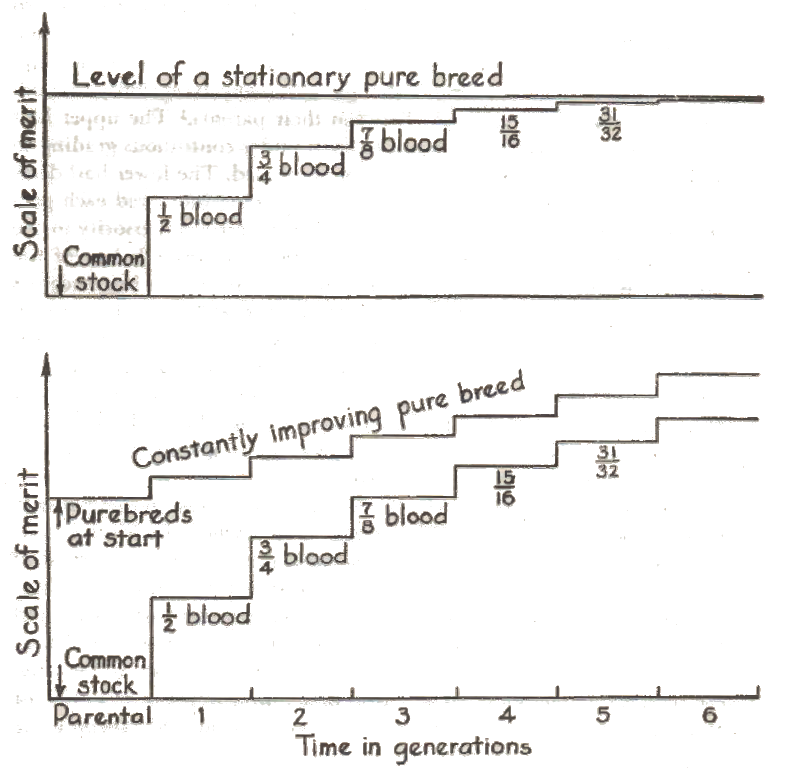
\includegraphics[width=\textwidth]{Figure_2.png}
    \caption{The contrast between grading to a pure breed which is stationary in merit and grading to a pure breed which is improving its merit by a constant amount each generation.}
    \label{fig:Lush_Figure_2}
\end{figure}

The very fact that the purebred has generally been found useful in \index{Grading}grading up common stock carries with it the necessity 
for the continued improvement of the purebred itself if the distinction between pure breds and grades is to be maintained. 
If the pure breed did not continue to improve, the average merit of the grades would soon be so nearly equal to that of the 
purebreds that the distinction between them could not long be maintained. Figure~\ref{fig:Lush_Figure_2} illustrates this on the assumption
(which is true in general, although with many exceptions) that offspring average about half way between their
parents.\footnote{Allowance for regression toward the mean of the groups from which the parents were chosen needs to be 
made if the parents were selected individuals. Also \index{Heterosis}\textit{heterosis} sometimes causes the first-cross generation to be 
better than the diagram indicates.} The upper half of the diagram shows what would happen under continuous grading to a 
pure breed which was not itself being improved. The lower half deals in a similar way with a pure breed which is being 
improved each generation by an amount equal to one-tenth of its initial superiority to the common stock. The difference 
betwen upper and lower halves of the diagram is not important in the first generation or two but becomes 
pronounced after several generations of grading and shows how a continuously improving breed may maintain a commercially 
important margin of superiority over its grades as long as it can continue its own improvement. The diagram, of course, is 
simpler than the facts (as will be seen in more detail in the chapters on selection); but it demonstrates the necessity of 
continued breed improvement to maintain the superiority and popularity of the purebred sire.
\index{Purebreds, superiority of|)}

\index{Making new breeds|(}
Animal breeding history in the United States may be divided into four periods. First, there was a pioneer period when the 
kind of livestock was not of much importance. \index{Making new breeds}Second, there followed a period of developing local races and a little 
experimenting with introduced breeds. Third, came a period of extensive experiments with introduced breeds and widespread 
expansion of organized pure breeding characterized by rivalry between breeds and by breed promotion. In the present period 
the dominant interest is in breed improvement, not only for successful competition with the other breeds, but also for 
keeping the purebreds distinctly ahead of the grades of the same breed in order to maintain a steady demand for purebred 
sires. These periods did not begin and end suddenly but merged gradually into each other, and some of the elements which 
characterize each period were present in lesser degree in all periods. At present it seems likely that plans for
breed improvement will go on within the framework of the existing systems of purebreeding, but here and there occurs some 
experimenting with the combination of more or less blood from two or more breeds, just as was done by some of the breed 
founders in the days before strictly pure breeding and registration became the standard methods of improved breeding.
\index{Making new breeds|)}
\chapter{The Relation of the Breed Association to Breed Improvement}
\label{cha:relationship-breed-association-breed-improvement}
\index{Breed associations|(}

The activities of the breed associations are intended to maintain the present merit of the breed, to improve the merit of the breed, and to promote the business interests of the members. Some activities serve all three of these purposes, and many serve two of them.

The primary object of breed associations, particularly in countries to which the breed is not native, is to safeguard the 
\index{Breed purity}purity of the breed and to furnish accurate pedigrees to all breeders who desire them. In practically all cases the breed 
association took over the conduct of the herdbook early in the history of the association. Most of the clerical work in 
most associations is used for issuing and checking the accuracy of registrations and transfers. Most of the errors 
discovered in applications for registry or transfer are matters of carelessness or neglect, but close watch is kept for 
fraud, and occasionally a member is expelled for this reason or his registrations are canceled. Because of the possibility
of legal complications and internal dissension, this is not usually done unless the proof is quite conclusive. The accuracy 
of a pedigree depends mainly upon the honesty and carefulness of the man who signs the application for registry. But the 
breed association's policy of rejecting or returning applications not accurate in detail and of investigating within 
reasonable limits cases where fraud is suspected prevents many errors which would come into pedigrees if there were no such 
supervision. Some associations publish the facts when a member is expelled or registrations are canceled because of fraud. 
Others keep it quiet to avoid scandal. Probably the first policy is generally the wiser. In either case the news usually 
spreads fast. Safeguarding the purity of a breed does nothing to increase its merit but does act to some extent as a ratchet
mechanism to maintain whatever special merit the breed already has and to hold any future improvements which may be made in 
its average merit. Preserving the present merit of the breed is particularly important if the breed is an introduced one, 
few in numbers, and surrounded by animals of distinctly different origin.

\index{Shows and fairs|(}
A breed association tries to \textit{improve} the merit of the breed by guiding the ideals which the breeders use when making their 
selections and by making official tests or ratings of the productiveness or conformation of individual animals. The ideals 
of the breeders are influenced by such activities as adopting a score card\index{Score cards}, or other verbal description of the breed ideal, 
or a series of ``true type''\index{``True type'' models or pictures} pictures or models. A different approach to the same goal is through control of judging 
standards at the various fairs. Sometimes that amounts only to advising the fair management upon request whether the breed 
association considers a certain individual competent to judge that breed. In other cases the breed association prepares a 
fairly small list of men considered competent, and its contributions of prize money are contingent upon the fair management's
selecting its judge from that list. Sometimes the association prints circulars or uses advertisements which serve the 
double purpose of promoting wider interest in the breed and showing pictures of animals which are considered nearly ideal 
for that breed. The association sometimes instructs its members as to what is considered important in pedigrees (See 
example in \textit{Holstein-Friesian World}, 33: 300, April 4, 1936).

The general purpose of all these ways of teaching the breeders the official ideals for that breed is that the breeders thus 
informed shall follow those standards when making their own selections and cullings and will thus move the breed average 
nearer to the breed ideal. The breed association's efforts end with presenting the lesson to the breeder. Unless he asks 
for further help from the fieldman or other officer, it is entirely up to him whether he accepts the official ideal and how 
much or how little he uses it when making his selections and cullings.

Official tests of the speed of individual horses were characteristic of the Thoroughbred and the Standardbred from the very 
beginning. In the case of the latter, a certain speed was necessary for registration hence the name of the breed. As long 
ago as 1832 the preface to the list of Thoroughbred horses in Prussia contained the statement: ``Unless herdbooks contain 
production tests\index{Production testing|(}, they will be useless and without interest, since they will contain only names, of which no one knows
anything and which mean nothing.'' (Engeler, 1936). Official testing of dairy cattle began around 1880\footnote{Pages 15 and 
16 of \textit{Holstein-Friesian History}, by Prescott, Price, Wing, and Prescott.} with the Holstein-Friesian breed in the
United States, largely as a result of the work of Solomon Hoxie. (Private production records were being kept at least as 
long ago as the time of Thomas Bates.) For a number of years there were serious doubts as to whether official testing would 
become popular enough to be retained. However, it eventually proved so useful, not only for breed improvement but also as 
an aid in advertising and selling, that no dairy breed association would now try to do without its department of official 
testing. But such official tests are not yet a prerequisite to registration. Whether the breeder will test or not is still 
entirely voluntary with him, except as the demands of a considerable portion of his customers put some economic compulsion 
on him to test.

In the United States, official inspection of whole herds, with a rating of each animal for type, was begun on a voluntary 
plan in 1929 by one of the dairy breeds and has since been adopted by most of the others. This plan was used by only a few 
breeders during the depression of the 1930's but now seems to be spreading more rapidly. Type inspection or scoring, 
sometimes on a compulsory basis, has been practiced much longer in some other countries; for example in The Netherlands or
Switzerland.

Many of the swine associations have required the man who registers a litter to report the number of pigs farrowed and 
raised. Some have published in the herdbooks the number farrowed in each litter. Recently Records of Performance have been 
established by several of the swine breed associations, the Hampshire having been the first. These are based mostly on 
weight of litter weaned at 56 days. They are still voluntary and are just beginning to be tried on an extensive scale. They
seem to be a sound step forward, but their wide adoption will probably depend on how insistently the breeder's customers 
ask for such information when they come to buy boars.

Tests for measuring the practical productiveness of beef cattle are being studied at experiment stations,\footnote{See Montana
Agr. Exp. Sta., Bul. 397; also Minnesota Agr. Exp. Sta., Tech. Bul. 94; also \textit{Empire Jour. of Exp. Agriculture},
8:259--68.} but these have not been adopted by any of the beef breed associations.

There have been some discussions of a Record of Performance for sheep, particularly for the fine-wool breeds. The shearing 
records made in New England a century ago were a kind of crude beginning in that direction. No definite plan is in actual 
operation today.

Although there has been some experimenting with endurance rides for cavalry horses and with pulling tests for draft horses, 
these have not yet been made an official part of breed association activities.

The associations in the United States do not usually keep official lists of the prizes won by individual animals at the 
important shows, although some of them do so in an unofficial way. In many cases the breed paper performs that service.
\index{Production testing|)}

With a very few exceptions --- such as the speed requirement for the Standardbred horse, the type\index{Type classification} inspection given to Brahman cattle which are admitted as foundation stock, and the flock inspections which are a part of some plans of poultry improvement --- the purely voluntary nature of the production-testing and type-rating done under the auspices of the breed associations in the United States is like that in Britain, but is in marked contrast to the compulsory inspections or testing
in some breeds in continental Europe. Those are discussed in more detail in the chapter on selective registration\index{Selective registration}. In considering how far it would be possible or wise for the American associations to go in that direction, there are broad general questions as to how far collective policies and efforts can or should replace or supplement individual freedom
to follow whatever \index{Breed papers|(}breeding policies or use whatever purebred animals one pleases, without regard to whether those would be
approved by a majority of one's fellow breeders or by an official inspector of the association. Besides such questions of 
general principle, there are also some immediately practical questions of expense which might make impossible, in breeds as 
widely scattered as many of those in the United States, procedures which are feasible in lands where the breed is highly 
concentrated in one or a few localities. Most directors of the breed associations in the United States are reasonably eager 
to adopt any new practices or requirements which will increase the merit of their breed faster than at present. They 
usually demand that the new plan shall be tested in actual operation, however, before they commit their association 
definitely to it. They have sometimes tried a plausible scheme only to find that it did not work as well as they had felt 
sure it would, and traces of the confusion and discontent which resulted have remained for years to plague them.

Naturally, many activities of the breed association are directed mainly at promoting the present business interests of the 
members. Examples are the efforts to expand the breed numbers by getting new breeders to establish herds, the promotion or 
management of sales and the correspondence which the secretary's office has with would-be purchasers of breeding stock. 
Most associations prefer to give support and encouragement to sales efforts but not actually to manage the sale themselves
lest the dissatisfactions which inevitably arise about some transactions should result in animosity toward the association 
itself.

The provision of prize money at the more important shows is intended to promote the breed by bringing out larger numbers, 
thus giving more advertisement to the breed. It is also intended to improve the breed by teaching more people the ideal for 
that breed.
\index{Shows and fairs|)}

Many of the larger breeds have one or more papers devoted mainly to promoting the interests of the breed. Most of these 
breed papers are privately owned and managed, but some are owned and operated by the association itself. The contact 
between the association and the breed paper is close and important to both parties, even when the paper is privately owned. 
Most of the activities of the breed paper are devoted to the immediate business interests of the members --- advertisements 
and news of sales, merchandise for breeder's needs, etc. --- but some of these papers carry articles and information helpful 
in improving the merit of the breed, but not otherwise a matter of financial profit to anyone. Besides the breed papers, 
most associations print leaflets, buy advertising space in other magazines which reach stockmen, and make occasional use of 
the radio as part of their regular efforts at breed promotion.

The activities of the fieldmen or breed extension service are in considerable part devoted to expanding the numbers of the 
breed and helping new breeders get started. The fieldmen work also with boys' and girls' clubs and help established 
breeders with their problems. 

The forms of government of the breed associations vary widely. Usually the policies are determined by an unsalaried board 
of directors, preferably with overlapping terms and only one-third elected each year to prevent erratic changes in 
policies. The executive work of carrying out those policies is administered by a paid secretary. Sometimes there is a fixed 
number of shares of stock, as in most industrial corporations, and one can become a stockholder only by buying a share from 
someone else. More often the number of shares is not limited but any breeder approved by the board of directors may become 
a member by paying a fixed (usually small) sum for a non-transferable membership. Sometimes all members present at the 
annual meeting can vote. In other associations members not present can vote by proxy. Other associations, especially those 
with large financial reserves, have more or less elaborate systems of delegates or representatives chosen by districts, to 
ensure proportional representation and to avoid abuse of the proxy system. The form of government is important insofar as 
it may promote or endanger stability in conducting the association's activities, make it easy or difficult for the board of 
directors to see that the secretary carries out the general policies they wish, and make it easy or difficult for a minority
to seize and hold control. Some of the cases where there are two or more associations for the same breed had their origin 
in intense dissatisfaction on the part of a group which was not in control, either because it was a minority or because 
control had been seized by another group which could not be ousted with the existing machinery for governing that 
association. At one time there were seven separate organizations recording Poland China pedigrees. The number was not finally
reduced to one until 1946.\index{Breed papers|)}

The current problems of the breed associations are numerous. Financial problems have been acute with many associations 
since 1920. Nearly all of the swine and sheep associations and some of the cattle and horse associations have suspended 
publication of their herdbooks. What the final substitute for the printed herdbook will be is not yet evident. In some 
breeds there are still two or more registration associations, with some duplication of operating expenses.

An innovation which is still in the experimental stage in the United States, although it was used by breeders of Thoroughbreds a century ago and advocated by Thomas Bates as a means of overcoming what he thought were defects in the conduct of the Coates Herdbook for Shorthorns, is the filing of \index{Birth certificates} birth certificates which act as tentative registrations. They keep the date of birth and the records of parentage straight but permit the owner to wait until the animal is mature to complete the registration. This is a common practice in those European associations which require inspection for conformation. Since such inspection must wait until the animal approaches maturity, records of parentage might become lost or incorrect in the interval if this precaution of filing a birth certificate were not taken. The increasing percentages which are incorrect when registration is delayed is illustrated by the following data\footnote{\textit{Holstein-Friesian World}, June 21, 1941, page 708.} on 19,172 Holstein-Friesian applications received during a six-weeks period.

\begin{table}[htbp]
	\centering
	\begin{tabular}{cc}
		\textsc{Age} & \textsc{Percentage Incorrect} \\
		Under 2 months  & 13 \\
		2--6 months & 21 \\
		6--12 months & 25 \\
		12--18 months & 33 \\
		18--24 months & 44 \\
		Over 24 months & 53 \\
	\end{tabular}
\end{table}

The Jersey association has recently experimented with selective registry and a pedigree rating system
(the ``star bull'' plan) for bulls. Several dairy associations are trying plans for calling attention officially
to unusually meritorious proved sires; for example, the Ayrshire approved sire plan, and the Holstein-Friesian
publication of sire indexes.

Herdbooks, as printed in the past, permit the tracing of pedigrees in only one direction; that is, one can learn from the 
herdbook what an animal's ancestors were but cannot find what offspring it had. Often a full list of an animal's offspring 
is more valuable than all that could be learned by studying its pedigree. Most breed associations maintain office records 
which will permit making such lists (at least from females), but those are not published. The nearest approach to published
lists of this kind is in the reports of official testing in the dairy breeds where the tested offspring of a given sire or 
dam may quickly be found. Usually little or nothing is published about the offspring which were not tested officially, 
although the Ayrshire association attempts to learn what became of each untested daughter of the bulls in its ``approved 
sire plan.''

In the United States the breed associations receive no direct financial support from the state or national governments. 
Correspondingly there is no governmental control or supervision of the associations or their activities, beyond whatever 
legal regulations apply in general to all nonprofit corporations or associations. However, the representatives of the 
United States Department of Agriculture and of the state agricultural colleges cooperate in many ways with the breed 
associations in activities which are expected to improve the practical merits of the breeds or to benefit the buyers of 
purebred sires. Examples are the supervision of official production tests for the dairy breeds, helping in the management 
and promotion of livestock shows, conducting purebred sire campaigns, promoting the use of proven sires, etc. In some 
countries the governments extend considerable financial aid and correspondingly exert some control over association 
policies. The details of such arrangements vary widely. Examples are Switzerland, The Netherlands, and (especially since 
1936) Germany. In other countries, such as Canada and the Union of South Africa, the government cooperates in supervising 
registration and printing the herdbooks but does not participate in or control other activities of the associations. In yet
other countries, such as Denmark and Argentina, the herdbooks are conducted by farmers cooperatives or by a ``Rural 
Society,'' and the breed association either does not exist or is an advisory and promotional body.
 
Most of the breed \textit{improvement} has to be done by the breeder himself. The association stands ready to help and 
advise him, but it does not select the animals he shall use or decide which he shall cull, except in the comparatively few 
cases where animals are barred from registry because they possess some undesired characteristic. Nor does the association
decide which males shall be mated to which females. The actual selections and the choice of a mating system are left almost 
entirely to the individual breeder to do as he sees fit, provided his animals are purebred and the correctness of their 
pedigrees is unchallenged. Breed associations must remain more or less responsive to the opinions of the majority of the 
breeders and therefore cannot be expected to do much pioneering or testing of new and unpopular ideas. This will have to be 
done by venturesome breeders or by public research institutions. Practical experience indicates that breed associations are 
necessary for breed improvement, since practically every breed which has persisted long has soon developed an association 
to look after its interests. Yet the association's part is on the whole the conservative one of helping hold whatever 
average merit the breed has already attained and acquainting the beginner and the public with what is considered ideal by 
most breeders of that breed. Most of the aggressive positive work toward improving the merit of the breed to still higher 
levels will have to be done by individual breeders who are unusually able, energetic, persevering, or lucky.
\index{Breed associations|)}

\section*{REFERENCES}

\begin{hangparas}{0.5in}{1}%
Anonymous. 1930. ``Notice-Registration Cancelled.'' Holstein-Friesian World,
27 (No. 24):1177.

Advanced Registry Office. 1936. Pedigrees. Holstein-Friesian World, 33:300.

Engeler, W. 1931. Studies on the development and situation of pedigree registering
in the cattle-breeding industry. 92 pp. Internat. Inst. of Agr., Rome.

---. 1936. Die Entwicklung des Herdebuchwesens unter dem Einfluss der Lehren von der Vererbung
und Z\"{u}chtung bei den landwirtschaftlichen Haustieren. (In) Neue Forschungen in Tierzucht. Bern.

Peterson, Guy A. 1919. Swedish herdbook registration. Hoard 's Dairyman, 74:62.

Plumb, Charles S. 1930. Registry books on farm animals.
 
Van den Bosch, I.G.J. 1930. The Holstein industry in America. The scoring system in the Netherlands. 
Holstein-Friesian World, 27:283 and 337.

Wilson, C. V. 1925. A study of the breeding records of a group of Shorthorn cows. West Virginia Agr. Exp. Sta., Bul. 198.

Early volumes of the herdbooks of the breeds in which you are interested. Read especially the minutes 
of some of the early business meetings.
\end{hangparas}

%\textsc{Genetic Principles of Animal Breeding}
\chapter{The Mendelian Basis of Inheritance}
\label{cha:mendelian-basis-of-inheritance}

\section*{PARTICULATE AND DUPLICATE NATURE OF INHERITANCE}

The essence of Mendelism is that inheritance is by particles or units
(called genes hereafter) and that these genes are present in pairs, one
member of each pair having come from each parent. Each gene maintains
its identity generation after generation instead of blending with
the other genes to form a new kind or blend of
\index{``Blending inheritance''}hereditary substance, as
was thought in pre-Mendelian days. When the individual reproduces,
it transmits to each offspring one or the other, but not both, of the
genes in each pair it possesses. thus the parent gives to each offspring
\textit{only a sample half of its own inheritance}. The laws of chance govern
this sampling, subject to the restriction that each sample must contain
one gene of every pair. This sampling nature of the process of inheritance,
scarcely suspected in pre-Mendelian days, allows a parent to transmit
different inheritance to different offspring. More precisely, if we
let \textit{Aa} represent a pair of genes in a parent which has two offspring,
there is one chance in four (the exact result in individual cases varying,
of course, according to the laws of sampling) that both offspring will
get \textit{A}. There is one chance in four that both will get \textit{a} and there are two
chances in four that one will get \textit{A} and the other will get \textit{a}. Similar
probabilities apply to every other pair of genes. Thus, about half of the
genes which two offspring receive from the same parent (i.e., about
one-fourth of all the genes they have) are exact duplicates; but the
other genes the two get from that parent (another fourth of all the
genes they have) were opposite members of the pairs in that parent. In
those pairs of genes for which the parent was homozygous it will not
matter which gene of the pair is transmitted, for the result will be the
same with either. Most parents are heterozygous for many pairs of
genes. Here lies the explanation of the fact that identical pedigrees do
not mean identical inheritance, although they usually do mean a considerable
degree of likeness.\footnote{To illustrate the Mendelian basis for the fact
that identity of pedigree generally means similarity but not identity of
inheritance, let us consider the probable results of a particular mating in
a breed heterozygous for many pairs of genes and mating at random with
respect to each pair. If the contrasting alleles in each pair are equally
frequent in the breed, then the most probable Mendelian formula of mates
chosen at random can be illustrated as below, the mates being alike in some genes
and unlike in others. How many different kinds of full sibs could there be from this
particular mating? How many different kinds of half sibs could come from this one sire
(or dam) mated to all the different kinds of mates which exist in the breed? How many
different kinds of individuals can exist in the entire breed? The Mendelian formulae
of the parents and the answers to each of these three questions may be indicated as
follows:

Formula of sire: \textit{AABbccDdeeFfGGHhli]jKKIIMMNnooPp}

Formula of dam: \textit{AABbCcDDeeffGgHhii]jKkLLmmNNOoPp}

Kinds of full sibs: lx3x2x2xlx2x2x3x2x3x2xlxlx2x2x3 = 20,736

Kinds of paternal half sibs: 2x3x2x3x2x3x2x3x3x3x2x2x2x3x2x3 = 1,679,616

Kinds in breed: 3x3x3x3x3x3x3x3x3x3x3x3x3x3x3x3 = 43,046,721

Since there are more than twenty thousand kinds of full sibs possible from this
mating, it is unlikely that two full sibs even from among a large number would happen
to be exactly alike. Yet less than one two-thousandth of the total number of kinds
of individuals possible in the whole breed are possible at all in this particular set of
full sibs. This sire could not possibly sire a twenty-fifth of the kinds possible in the
whole breed, no matter what kind of mates he had. This example is schematic in two
important respects: first, many more than 16 pairs of genes are doubtless heterozygous
in all breeds; and, second, it would be a surprising coincidence if the unlike
alleles were equally numerous in more than a few of those pairs.} That identity of pedigree
(as of full brothers) does not mean identical heredity was well known in pre-Mendelian
days but either was regarded as one of the unexplained mysteries of
heredity or interpreted to mean that a large amount of entirely new
inheritance (mutations we would say today) had arisen in each individual.
\index{Genes, nature of}

\index{Sampling nature of inheritance|(}
Since half of the inheritance comes from each parent, except in the
case of sex-linked genes, and since in each pair the gene received from
the sire and gene received from the dam are equally likely to be transmitted
to any one offspring, most of the facts of inheritance when
expressed in quantitative form involve the fraction l/2. It is only a
small exaggeration to say that the mathematics of genetics is the algebra
of 1/2!

\index{Allele}\index{Dominance}Dominance is not an essential part of Mendelism, although Mendel
himself noted it. It is a ready explanation of some cases of ``reversion''
or \index{Atavism}``atavism,'' but not the only explanation for those. The chief part
played by dominance is to increase the variability of the population
slightly and to make certain genotypes indistinguishable from each
other. There is nothing in the mechanism of inheritance which would
cause a dominant gene to increase in numbers at the expense of its
recessive allel, or the reverse. \index{Gene frequency}If \textit{q} is the proportion of \textit{A} genes and
$1 - q$ is the proportion of \textit{a} genes in the population and \textit{p} is the
proportion of heterozygotes, then no matter what system of mating prevails,
the zygotic ratio\index{Zygotic ratios} will be $(q - p/2)AA:p Aa: (1 - q - p/2) aa$.
If these have equal opportunity to reproduce (that is, if no selection for
or against either of the three genotypes prevails), then the proportion
of \textit{A} genes in the next generation will be $q - p/2$ from the \textit{AA individuals
plus} $p/2$ from the \textit{Aa} individuals which equals \textit{q} in the whole
population, the same as it was in the preceding generation. Without
selection the Mendelian mechanism itself does not change gene ratios
except, of course, that it permits sampling variations to occur in the
segregation process at each generation. Those are slight except in very
small populations. There they cause the phenomena of inbreeding.
\index{Sampling nature of inheritance|)}

\section*{POST-MENDELIAN ADDITIONS TO THE LAWS OF INHERITANCE}
\index{Linkage|(}

Mendel knew nothing of \index{Chromosomes|(}\textit{chromosomes} or \textit{linkage}. The achievements
of genetics in the last third of a century in identifying the
chromosomes as the carriers of the genes have not changed the laws
which Mendel discovered, except to modify the law of independent
assortment so that it is now known to apply only to genes which are on
different chromosomes. Cytological investigations of the mammals and
birds are unusually difficult because the number of chromosome pairs
is large, the chromosomes are small, and the processes of killing, fixing,
and staining are apt to cause the chromosomes to ``clump'' together, so
that the observer cannot be sure how many there are.

Because of these difficulties, mammalian and avian chromosomes
have not been so well investigated as those of most farm crops and of
many lower animals. In several cases investigators do not yet agree in
their counts. Some species have been studied by only one investigator.
Most of the findings quoted in table~\ref{tbl:Lush_Table_1} are still subject to confirmation.\footnote{For a
more complete list and references, see: Oguma, Kan, and Kakino, Sajiro.
1932. A revised check-list of the chromosome number in vertebrata. \textit{Jour. of Genetics},
26:239--54, and for birds: Miller, R. A. 1938. \textit{Anatomical Record} 70:156--58.}
Work much older than 1920 is quoted only where no subsequent work
has been reported, or where this earlier work has been quoted widely.
In general the later work is more apt to be correct. On account of the
``clumping,'' the larger numbers are more likely to be correct wherever
there is not yet substantial agreement.

Most farm animals have around 20 to 30 pairs of chromosomes;
hence two genes chosen at random will nearly always be independent of
each other. Yet if one is considering a trait affected by more than six or
seven pairs of genes, there is likely to be linkage among some of them.\footnote{The
chicken, the mouse, and the rat are the only farm animals for which the
construction of linkage maps is yet well along. See \textit{Jour. of Heredity} 3l:232--35 and
36:271--73. Some mapping has begun with the silkworm and with cattle.}
On account of linkage, genes which were transmitted to the parent
together (i.e., which both came to it from the same one of its parents)
will be transmitted together to the offspring more often than if they
were independent. Yet in the population as. a whole, if crossing-over
occurs at all, \index{Coupling and repulsion} the ``repulsion'' and ``coupling'' phases soon become equally
frequent, thus causing linkage to hinder selection (in a hitherto
unselected population) in about as many cases as it helps. Hence linkage
does not offer the breeder much chance to get one gene by selecting
another closely linked to it. The effects of linkage in causing two genes
or characteristics to be together or apart more often than not are conspicuous
only in the first few generations after a cross between two
unusually homozygous races-a condition which rarely confronts the
animal breeder under our present purebreeding systems. The existence
of linkage causes the genes to tend to segregate in large groups at any
one cell division and hence causes the population to behave as if there
were fewer genes than there actually are. But this effect is probably
unimportant, since the cross-overs in different cells, even in the same
individual, may be at various places on the chromosomes and since
genes with opposite effects are as likely to be linked together as are
genes with similar effects. Linkage is some hindrance to progress by
selection (after the first generation) since it keeps desired and undesired
genes from recombining into separate gametes as often as they
would if not linked. This lessens slightly the variability among the
immediate offspring of selected parents and consequently reduces the
amount which can be accomplished by selecting among them.

\begin{small}
	\label{tbl:Lush_Table_1}
	\setlength\LTcapwidth{\textwidth} % default: 4in (rather less than \textwidth...)
	\setlength\LTleft{0pt}            % default: \parindent
	\setlength\LTright{0pt}           % default: \fill
	\begin{longtable}{@{\extracolsep{\fill}}b{2cm}|b{2cm}|b{2cm}|b{4cm}}
		\caption{\textsc{Recent Reports of Chromosome Numbers in Mammals and Poultry}}\\
		\hline
		\hline
		Animal 				& Number of Pairs of Chromosomes & Heterogametic Sex & Investigator and Date of Publication \\
		\hline
		\endfirsthead
		\caption[]{\textit{Continued}}\\
		\hline
		\hline
		Animal 				& Number of Pairs of Chromosomes & Heterogametic Sex & Investigator and Date of Publication \\
		\hline
		\endhead
		Farm animals: 		&                     	&        			& \\
		\tabindent Horse    & 30                  	& Male   			& Painter, 1945 \\
		              		& 19                  	& Male   			& Wodsedalek, 1914 \\
		              		& 19                  	& Male   			& Masui, 1919 \\
		\tabindent Ass      & 32                  	& \ldots 			& Sokolov, 1937 \\
		\tabindent Mule     & Unpaired, 51 in all 	& \ldots 			& Wodsedalek, 1916 \\
		\tabindent Camel    & 35                  	& \ldots 			& Novikov, 1940 \\
		\tabindent Cattle   & 30                  	& Male   			& Krallinger, 1930 \\
	    	          		& 19                  	& Male   			& Wodsedalek, 1920 \\
	        	      		& 30                  	& Male   			& Makino, 1944 \\
		\tabindent Yak		& 30					& \ldots 			& Zuitin, 1938 \\
		\tabindent Buffalo	& 30					& \ldots			& Pchakadse, 1939 \\
							& 24					& \ldots			& Makino, 1944 \\
		\tabindent Sheep	& 27					& Male				& Berry, 1941 \\
							& 30					& Male				& Several workers, 1931 to 1940 \\
		\tabindent Goat		& 30					& Male				& Krallinger, 1931 \\
							& 30					& Male				& Warwick, 1935 \\
		\tabindent Swine	& 19					& Male				& Krallinger, 1936 \\
							& 19					& Male				& Crew and Koller, 1939 \\
		\tabindent Dog		& 26 $\pm$				& Male				& Painter, 1925 \\
							& 39					& Male				& Ahmed, 1941 \\
		\tabindent Cat		& 19					& Male				& Minouchi, 1928 \\
							& 19					& Male				& Koller, 1941 \\
		Farm poultry:		&						&					& \\
		\tabindent Chicken	& 33					& Female			& White, 1932 \\
		\hline		
		\tabindent Chicken	& 39					& Female			& Yamashima, 1944 \\
							& 40					& Female			& Miller, 1938 \\
							& 16 to 37				& Female			& Various authors since 1923 \\
		\tabindent Duck		& 38 to 39				& Female			& Werner, 1927 \\
							& 39					& Female			& Sokolov, \textit{et al.}, 1936 \\
		\tabindent Turkey	& 23 to 29				& Female			& Various authors 1929 to 1936 \\
		\tabindent Peacock	& 18 to 29				& Female			& Tiniakow, 1934 \\
		\tabindent Pigeon	& 31					& Female			& Oguma, 1927 \\
							& 25 $\pm$				& Female			& Hance, 1933 \\
							& 24 $\pm$				& Female			& Painter and Cole, 1943 \\
		Various mammals:	&						&					& \\
		\tabindent Man		& 24					& Male				& Many recent authors \\
		\tabindent Chimpanzee			& 24					& Male ?			& Yeager \textit{et al.}, 1940 \\
		\tabindent Old World monkey	& 27					& Male				& Painter, 1925 \\
		\tabindent New World monkey	& 27					& Male				& Painter, 1925 \\
		\tabindent Nyctereutes (raccoon dog)	& 21			& Male				& Minouchi, 1929 \\
		\tabindent Red fox				& 21					& Male				& Wodsedalek, 1931 \\
		\tabindent Fox:		&						&					& \\
		\hspace{6mm} V. vulpes			& 17					& \ldots			& Andres, 1938 and Wipf, 1942 \\
		\hspace{6mm} V. lagopus			& 26					& \ldots			& Andres, 1938 \\
		\hspace{6mm} V. fulva			& 16					& Male				& Bishop, 1942 \\
		\tabindent Rat		& 21					& Male				& Many recent authors \\
		\tabindent Mouse	& 20					& Male				& Many recent authors \\
		\tabindent Deer mice (Peromyscus) &	24 to 29		& \ldots			& Cross, 1938 \\
		\tabindent Rabbit	& 22					& Male				& Painter, 1926 \\
		\tabindent Rabbit	& 22					& Male				& Minouchi and Ohta, 1932 \\
		\tabindent Guinea pig			& 19					& Male				& Harman and Root, 1926 \\
							& 31					& Male				& League, 1928 \\
							& 33					& Male				& Mols, 1928 \\
		\tabindent Mink		& 14					& Male				& Schackelford and Wipf, 1947 \\
		\tabindent Hamster, golden		& 19					& Male				& Koller, 1938 \\
		\hline
		\tabindent Hamster, striped	& 7						& Male				& Pontecorvo, 1943 \\
		\tabindent Twelve other species of rodents	& 22 to 43 (only 3 above 27)	& \ldots	& Cross, 1931 \\
		\tabindent Peccary	& 15					& \ldots			& Krallinger, 1936 \\
		\tabindent Armadillo			& 30					& \ldots			& Painter, 1925 \\
		\tabindent Bat		& 24					& Male ?			& Painter, 1925 \\
		\tabindent Hedgehog	& 24					& \ldots			& Painter, 1925 \\
		\tabindent Opossum	& 11					& Male				& Hoy and George, 1929 \\
						& 11					& Male				& Painter, 1925 \\
		\tabindent Kangaroo	& 6						& \ldots			& Painter, 1925 \\
		\tabindent Eight other genera of marsupials	& 6 to 10	& Male	& Various authors \\
		\hline
	\end{longtable}
\end{small}

Mendel did not know of sex-linkage\index{Sex linkage} which, in the heterogametic sex, is an exception to the rule that
inheritance is in duplicate and comes equally from both parents. Only one pair of chromosomes carries
the sex-linked genes. Presumably something like one-twentieth or one-thirtieth of all the genes are
sex-linked, although that is only a rough approximation since the sex-chromosomes might carry more or
less than their proportionate share of the genes. To ignore sex-linkage will generally lead to but
little error; yet there doubtless is some sex-linkage in all farm animals, and probably there are
occasional characteristics which are affected by a disproportionately large share of sex-linked
genes. The general effect of sex-linkage is to make parent and offspring of opposite sex resemble
each other slightly more than parent and offspring of the same sex do. Here and there it has some
conspicuous special effect, such as making possible, in some matings, the identification of sex in
very young poultry. Partial sex-linkage is known genetically in man and presumably exists in all other
mammals in which portions of the X-chromosome cross over with portions of the Y-chromosome. The
practical consequences are like those of sex-linkage but even less noticeable.
\index{Chromosomes|)}
\index{Linkage|)}

\section*{IS THERE ANY NON-MENDELIAN INHERITANCE}
\index{Non-Mendelian inheritance|(}
\index{Polyploidy|(}

Each year of genetic research brings added evidence that all inheritance is Mendelian in the broad
sense of being in duplicate and particulate, with the particles maintaining their identity. The only
well-established exceptions are plastid inheritance, known only from plants, and polyploidy, where
inheritance is particulate but present in more than duplicate. Polyploidy seems to be very rare in
animals, although it appears to have been important in the evolutionary history of the plant kingdom.
On account of the sampling nature of inheritance, polyploidy must be a temporary condition lasting only
a few generations until the polyploid individuals either die out or develop a new diploid division
among their chromosomes. A few cases of inheritance through the maternal line only have been reported.
Most of those have later been found to require some other explanation. Often it is found by further
experiment that these were characteristics for which the unfertilized ovum was already organized and the
genes which the sperm brought are merely delayed a generation in expressing their effects. Whether the
shells of certain snails coil to the left or to the right is an example.

It may never be possible to prove rigorously that all inheritance is Mendelian in this sense, for so long
as the inheritance of any characteristic is unknown, an obstinate skeptic might still say: ``Perhaps the
inheritance of that characteristic conforms to some other rule.'' It is a fact, however, that many cases
of inheritance which were at one time thought not to behave in the Mendelian manner, have been shown by
more thorough analysis to behave in that very way except that the number of factors is large or that the
interactions between different factors are unusually complicated or that the egg was already so highly
organized that the genes in the sperm cell could not show some of their effects until the next generation.
Moreover, the ineffectiveness of selection within pure lines seems to be some positive evidence that there
can be no appreciable amount of truly ``blending'' inheritance. (Cf. Fisher, pp. 17--18.)
\index{Non-Mendelian inheritance|)}
\index{Polyploidy|)}

\section*{THE NUMBER OF GENES}
\index{Genes, number of|(}

There are at least four kinds of evidence which show something about the total number of pairs of genes in
certain species. They leave little doubt that the breeder of farm animals must contend with a genetic
situation in which the number of different pairs of genes heterozygous in his herd or flock is at least
many scores, probably many hundreds, and perhaps even a few thousands.

The first kind of evidence is the number of genes which have actually been found in the organisms studied
most. In \textit{Drosophila melanogaster} more than 500 different loci have already been located on the
chromosome maps, and many more are known. In \textit{D. pseudoobscura} there are in the third chromosome
alone at least 289 loci which can mutate to lethal genes (\textit{Genetics} 26:39). Baur and his co-workers
found some 300 genes in the snapdragon, \textit{Antirrhinum majus}. In corn (\textit{Zea mays}) some 400
genes had been catalogued up to 1935 (Rhoades and McClintock). In the wasp, \textit{Habrobracon juglandis},
about 100 mutations at separate loci are known. In \textit{Datura} (the genus which includes the Jimsonweed)
about 500 genes were known, 77 of them located on the chromosome map, by 194l. The inherilance of more than
100 characters has been studied in barley (\textit{Genetics} 28:419). In man more than 200 genes have been
reported, some 45 of them on the X-chromosome, but the evidence for many of those is scanty because controlled
experimental matings are not possible. The number of genes reported for most species of farm animals is only\
a few dozen,\footnote{For example, Ibsen in 1933 listed 17 pairs of genes and one multiple allelic series of
genes affecting color in cattle. He mentions several other color characteristics, the mode of inheritance of
which was not yet clarified. In the fowl 21 genes are already (1940) located in six linkage groups
(\textit{Jour. of Heredity} 31:231--35), and other genes are known but not located.} and many of those are not
very certainly established, but only a few thousand farm animals have been observed under such circumstances
that genes would have been identified readily.

This kind of evidence has two limitations: First, only genes with effects conspicuous enough to permit their
ready identification can be catalogued in the Mendelian manner. Genes with minor effects can only be lumped
together in an indefinite background of ``modifying factors.'' Second, the number already found provides
scarcely any basis for guessing whether that number is only a tiny fraction or a large fraction of the total
number which exists. Certainly the number reported is less than the actual number.

A second kind of evidence comes from cytology. Work (\textit{Journal of Heredity} 33:403--7, 1942.) on the
\index{Chromosomes}chromosomes in the salivary glands of Drosophila shows about 5,000 distinct bands; and the cytogenetics of
deletions, inversions, etc., makes it seem plausible that each of these is a gene, although it remains
possible that there may be several genes in some bands. Belling in studying the chromosomes of the lily was
able to distinguish about 2,200 to 2,500 ``chromomeres,'' or distinct segments of its chromosomes; but the
genetics of the lily is not well enough known to show how closely the genes and the chromomeres correspond
to each other. Each chromosome in the farm animals surely must carry many genes; but the cytology of mammals
and birds is difficult and little except number is known of it so far.

A third kind of evidence comes from some indirect reasoning, based on the number of times certain mutations\index{Mutations}
recurred. The first such estimate was a figure of about l,800 loci, but it was recognized that the
assumptions involved made this lower than the true figure. Gowen and Gay in 1933 reached an estimate of
14,280 loci in Drosophila. This estimate had a large sampling error but was thought to have no consistent
bias either in the direction of largeness or of smallness. Muller and Prokofyeva in 1935 reached the
conclusion that in Drosophila the total number of loci ``\ldots is of the order of a few (ca. 5--10)
thousand.''

A fourth kind of evidence comes from the experiments on quantitative inheritance\index{Quantitative inheritance} which require for their
interpretation a minimum number of genes if those express their effects in the very simplest way (i.e.,
without dominance or other nonadditive interactions). Sumner's experiments with mice of the genus Peromyscus
showed that many of the quantitative characteristics in which two varieties or local races differed were
each affected by many genes for which neither population was homozygous. ``Student'' interpreted the Illinois
Agricultural Experiment Station's work in selecting corn for high and for low oil content as showing that the
oil percentage in the initial stock of corn ``\ldots was conditioned by the presence, or absence, of a number
of genes, at least of the order 20-40, possibly of 200-400, and not at all likely to be of the order 5-10.''\index{Selection}
The Illinois Station's work with the Bowlker herd, which was produced by crossing Guernseys and Holstein-
Friesians, has been interpreted (page 123, Annual Report for 1928--29) as requiring more than 10 pairs of
genes to explain the \index{Breed differences}breed difference in milk yield and several more pairs of genes to explain the breed
difference in the percentage of fat. The Tranekjaer experiments with Jersey and Red Danish cattle in Denmark
indicate that at least seven pairs of genes were concerned with the difference in fat percentage between those
breeds.\footnote{Wriedt postulated that one pair of genes would account for the breed difference; but, as
Skovsted pointed out, not enough of the parental types reappeared in the back-crosses or in the $F_2$ to justify
that. The figure seven mentioned here is based on comparisons of parental means and $F_1$ , $F_2$, and back-
cross variabilities.} Jull concludes that in the fowl sexual maturity, rate of laying, and persistency of laying
are each ``\ldots affected by a relatively large number of genes, some of which probably influence more than one
character.'' Many other examples might be cited, each yielding figures of from 4 or 5 up to more than 20 as the
minimum number of pairs of genes affecting a given quantitative characteristic.

The usual result of an experiment on the genetics of a quantitative
characteristic is that the number of genes involved ``cannot be less
than'' a certain number, but might be larger. Usually the longer the
genetic investigation continues, the more genes are found. In such
experiments the evidence which throws light on gene number usually
involves differences between the parental means and between the variabilities
of the parental groups, the $F_1$ or the $F_2$ or the back-crosses, or it
concerns the change produced in the mean and in the variability by a
given amount of selection. Often the numbers are small and the sampling
errors are high. Those may make the answer obtained either too
large or too small. Nearly all other sources of error make the answer
smaller than it should be. Thus, this kind of evidence can only show
that the number of genes is more than a certain small number which,
however, is usually too large to leave any reasonable hope that even the
most thorough study will enable a breeder to know the Mendelian
formula for all the important genes in any of his animals.

\index{Genes, nature of|(}
A fifth line of reasoning, which perhaps scarcely deserves to be called
evidence until more is known about the physiology of how the genes
produce their effects,\footnote{See \textit{Quart. Rev. of Biology}
13:140--68 and \textit{Physiological Reviews} 21:487--527.} is that the
development and functioning of each
organ in the animal is so complex and is dependent upon such a delicate
interplay of various tissues, hormones, fluids, etc., each acting at
the proper time, that it is scarcely conceivable that a small number of
genes can initiate and control all of this. The term ``unit character''\index{Unit character}
which was freely used in the early days of genetics tends to be avoided
now, lest it confuse by implying that one gene by itself is enough to produce
the whole characteristic. The gene, not the characteristic, is the
unit of Mendelism. In a sense it may be legitimate (and it is often convenient)
to refer to \textit{the contrast} between two characteristics --- for example,
red eye and white eye in Drosophila --- as a unit character since, in
some matings at least, the difference between the two characteristics is
caused by a difference in only one pair of genes. Yet it is confusing to
speak of \textit{red eye} as a unit character, since more than 40 genes have been
found thus far which must all be present if the usual red eye of the wild
fly is to develop. If one of them is absent, the eye may be ``purple''`; if
another is absent, it may be ``peach''; etc.; but the co-operation of them
all (and doubtless of still unknown genes) is required to produce the
normal eye. The cooperation of at least 100 genes is necessary to
produce normal green chlorophyll color in corn. (\textit{Amer. Nat.} 80:431).

The fact that many distinct abnormalities and defects are caused by
a change in only one gene is to be expected if that gene interrupts, at
some important stage for which there is no substitute, the long chain of
physiologic processes by which the normal characteristic usually develops.
For example, in the normal process of horn formation in cattle
there may be several stages which, if interrupted, would alter or prevent
all the later stages of development; but it is not easy to imagine that
any one gene could guide the whole course of horn development,
including the growth of the bony core, the blood vessels, nerves, etc.
Thus, it may be legitimate to speak of a single gene for hornlessness:
but it is not legitimate to infer that the allelic gene to that one is the
gene which produces horns. The case is analogous to that of destroying
a house by a single act, such as applying a match to it at any one of a
number of places. But a house can be built only by the timely co-operation
of an enormous number of individual acts. It is scarcely legitimate
to speak of refraining from applying the match as an act which builds
the house.

The eradication of single-gene defects, such as lethals and semilethals,
may be an important part of the task of animal breeding; but its
practical importance can scarcely approach that of changing the fertility,
vitality, growth rates, proportions of conformation, milk production,
speed, wool production, etc., which are most of the economic
differences between ordinary or moderately inferior and distinctly
superior animals. The genetic evidence indicates that these are complex
physiological characteristics i zn which most of the hereditary
differences are caused by a large number of genes, each with an individually
small effect.
\index{Genes, nature of|)}

\section*{CONSEQUENCES OF THE LARGE NUMBER OF GENES}
\index{Gametic ratio}
\index{Variation!as affected by gene numbers|(}

When only one pair of genes is concerned, two kinds of gametes and
three kinds of genotypes are possible. If there are two pairs of genes,
each possibility for the one may occur in combination with each possibility
of the other, thus permitting four kinds of gametes and nine
kinds of genotypes. Three pairs of genes permit 8 kinds of gametes and
27 kinds of genotypes. The general formulae are: the number of kinds
of gametes or of homozygous genotypes possible with n pairs of genes is
$2^n$ (which may be written $10^{.301n}$; the number of different kinds of
genotypes possible is $3^n$ (which may be writen $10^{.477n}$). These numbers
become big beyond human comprehension if \textit{n} is very large. Even if
there are only 100 pairs of genes, 31 digits will be needed for writing
the number of kinds of gametes possible; and there will be 48 digits in
the number of kinds of genotypes possible. The possibilities for hereditary
differences under this system are enormous. They may be visualized
by comparing them with the number of animals of each species
actually alive in the whole world at any one time. During the years
around 1926 to 1935 these were as follows for man and for some of the
more important farm animals (figures from USDA Yearbooks):

\begin{table}[htbp]
	\centering
	\begin{tabular}{lr}
 						& \textsc{Tens of Millions} \\
		Human beings	& 200 \\
		Cattle			& 70 \\
		Horses			& 10 \\
		Mules and asses	& 3 \\
		Sheep			& 69 to 74 \\
		Swine			& 25 to 28 \\
		Chickens (in the United States only)	& 44 \\
	\end{tabular}
\end{table}

Hence, if the number of different genes heterozygous in each species
is as large as 40 (and it may well be thousands), the number of different
hereditary combinations possible in each species is millions on millions
of times as large as the number of animals which can actually be alive
at any one time. It would be a remarkable coincidence if any two living
things were exactly alike in all their heredity, except for a few special
cases such as identical twins, asexually reproduced organisms, and possibly
members of a strain which had been very highly inbred for a long
time. Gesell says (\textit{Science} 88:227): ``Even in the detailed studies of animal
respiration, it has been found that no two dogs breathe exactly
alike.''

\index{Multiple alleles|(}
Another comparison to show vividly the enormous number of different
kinds of individuals possible is furnished by the physicists' estimate
that the number of electrons in the universe is about $10^{80}$. In a
species in which only 200 pairs of genes are heterozygous there could be
$10^{95}$ different kinds of individuals. This is a million billion times as
many as there are electrons in the universe!

In these calculations it was assumed that there are only two allelic
genes in each series. In several cases it is already known that there are
three or more different kinds of genes in an allelic series (called ``multiple
alleles'' in genetics), and it is possible that all allelic series are potentially
multiple.\footnote{Several series have already been found in which there are more than four
alleles. The albino series in the rabbit is an example. The maximum numher yet
reported in any organism is 45 alleles for a self-sterility gene in one of the primroses,
\textit{Oenothera organensis}. \textit{Genetics} 26:469. More than 22 alleles are known in the white
eye series in \textit{Drosophila melanogaster} and more than 40 at the locus for ``bobbed.''
In man at least four alleles exist to determine the blood types. $A$, $A^1$, $B$, and $0$, and
more than a half dozen alleles at the locus for the \textit{rh} blood factor have been reported.}
This increases the number of kinds of gametes and
genotypes possible. If \textit{m} alleles are possible in each of \textit{n} allelic series,
the number of different kinds of gametes possible is $m^n$ and the number
of different kinds of genotypes possible is $ \left[ \frac{m(m+1)}{2} \right]^2 $.

Linkage\index{Linkage|(} does not affect the number of kinds of gametes which may
be produced but does affect their proportions and thereby increases the
size of population necessary to permit all kinds of genotypes to be produced.
Also, it increases the number of genotypes possible because the
multiple heterozygotes will now be different genotypes according to
whether the linkage is in the coupling or repulsion phase. That is, $\frac{AB}{ab}$
and $\frac{Ab}{aB}$ will be different genotypes if linkage exists, whereas both
would have been the same genotype, \textit{AaBb}, if there had been no linkage.
A triple heterozygote, where all three genes are linked, can exist
in four different genotypes, a quadruple heterozygote in eight genotypes,
etc.

Both these additional complications --- multiple alleles and linkage --- increase
the number of kinds of genotypes possible. Unless the number
of heterozygous genes is very small, there is no escaping the conclusion
that the number of genetically different kinds of individuals possible in
a breed or species is practically infinite. Except in the rare case of identical
twins, one can confidently expect to breed cattle, or any other
species of farm animal, a lifetime without ever having a second animal
exactly like one he produced earlier.

If each gene had a different kind of effect and there was no confusion
by environmentally caused variations or by \index{Dominance}dominance, the number
of kinds of animals different in appearance or performance would
be the same as the number of kinds of genotypes. If all pairs of genes
showed complete dominance, but each pair of genes had a different
effect, the number of kinds of animals would be the same as the number
of kinds of gametes. But if very many genes are involved, some will
produce effects like those of others, some will produce effects only when
certain others are present, and some will produce the same effects as
variations in environment do. Therefore, if the genetic situation is at
all complicated, the outwardly distinguishable kinds of animals grade
into each other in an almost continuous series. When we classify a large
group of animals on the basis of outward appearance or performance
in any one characteristic, even with considerable precision, we are
almost certain to include in each class many genetically different kinds
of individuals.
\index{Genes, number of|)}
\index{Linkage|)}
\index{Multiple alleles|)}
\index{Variation!as affected by gene numbers|)}

\section*{THE GENETIC INTERPRETATION OF THE ``PURITY'' OF PURE BREEDS}
\index{Breed purity|(}
\index{Heterozygosis|(}
\index{Homozygosis|(}

In animal breeding usage, purity of breeding refers to ancestry and
is not the same as the genetic term ``homozygosity,'' although there is
some slight relationship between the two. The purebred animal is one
whose ancestors all belonged to that same breed for as far back as is
required by the rules governing registration in that breed. Since all
breeds are finitely limited in the number of animals alive at any one
time, and many breeds were very small in numbers for a long time during
their formative period, a certain amount of homozygosity was produced
by the resultant inbreeding\index{Inbreeding|(}. This is usually a faint force in
pure breeding as practiced today in breeds which have become large and
successful, but occasionally was intense during the formative period
when the breed was very small. The Shorthorn breed, which has the
oldest pedigree record, probably lost through the inbreeding process
about 25 or 30 per cent of its initial heterozygosity in the century and a
third from its foundation to 1920. Most of this was lost in the formative
stage while the ancestry of the future breed was largely included in the
herds of the Colling brothers, who both shaped their breeding operations
to an unusual degree around one bull, Favourite. In most breeds
yet studied, the breed is now losing something like one-half of one per
cent of its heterozygosis per generation. In breeds of cattle and sheep,
where the average length of generation is around four or five years, this
would mean that in a century the mere fact of absolute purity of breeding
would cause a decrease of about 10 per cent in the amount of heterozygosity
initially present. This would be partially offset by the
occasional registration of a grade through fraud, accident, or official
permission, and by the new mutations which might occur and survive
during that century. In addition to these three processes of inbreeding,
introduction of outside blood, and mutation\index{Mutations|(}, selection may have helped
either to increase or to decrease the average homozygosity of the breed.
Selection, however --- in marked contrast to its effectiveness in changing
average merit --- is a very feeble tool for changing homozygosity, except
under the very simplest genetic situations, as we shall see in chapter 11.
It is not likely, therefore, that selection has made much change in the
average homozygosity of the pure breeds since they were first separated
from the general population, although it has certainly changed the
breed averages distinctly in many cases.

\index{Selection}
It is sometimes argued that, while the total number of genes may
perhaps run into the thousands, yet most breeds (or subgroups of a
species in nature) will be homozygous for all but a few of those. This
seems improbable, since no genetic mechanism is known by which that
condition would be likely to be attained in the first place nor by which
it could be maintained very long if it ever were reached. If a breed or
species ever became entirely homozygous for a given pair of genes,
mutations --- even at a very low rate --- would cause that homozygosis to be
lost bit by bit. Selection is too feeble to restore complete homozygosity
as rapidly as mutation destroys it, especially if the mutations are usually
recessive, although selection is amply powerful to keep consistently
undesirable mutant genes from becoming abundant. Inbreeding can be
powerful enough to restore that homozygosity, but it is doubtful whether
it often is intense enough in nature or in the breeding of large and
popular breeds to achieve that end. Wright estimates\footnote{\textit{Genetics},
16:119--21. See also table 5 in Fisher's
\textit{Genetical Theory of Natural Selection}.} that a freely
interbreeding species of one million individuals at equilibrium with
one new mutation in each 1,000 individuals could support permanently
some 30,000 unfixed loci, which is larger than any of the current estimates
of total gene number. In other words, few genes in such a species
would be entirely homozygous all through the species. Smaller species
would not support so many\footnote{The same formula gives nearly 2,560 as
the number of unfixed loci in a species of 100,000 individuals, 210 in a species
of 10,000 and 16 in a species of only 1,000. Our ignorance of whether the rate
postulated for mutation is too high or too low and our ignorance of whether the
effective number of breeding individuals is far smaller or only a little smaller
than the census number prevent us from using these figures with much confidence.}
unfixed loci. The inbreeding which the pure breeds of livestock undergo comes
mostly not from the smallness of the breed in absolute numbers but from the
circumstance that many breeders are simultaneously using sons or grandsons of a
few currently famous sires.\footnote{See Calder's study of the Clydesdale breed
of horses. \textit{Proc. Roy. Soc. Edinburgh} 47 Part 2, No. 8:118--40. 1927.}
When the pure breeds finally reach equilibrium between the production of
heterozygosis by mutations and the loss of heterozygosis because the effective
number of animals in the breed is small, it is possible that the pure breed may
support only a few scores of unfixed loci. But it is unlikely that the pure
breeds have come at all close to that equilibrium point in the comparatively
short time (in terms of animal generations) since they were organized. It seems
entirely conservative to estimate that the average pure breed is still heterozygous
for hundreds of pairs of genes, although, of course, no animal in it is
heterozygous for even half of them and probably no one gene is heterozygous
in even half of the members of a breed.
\index{Breed purity|)}
\index{Heterozygosis|)}
\index{Homozygosis|)}
\index{Inbreeding|)}

\section*{MUTATIONS}

Mutation is a rare process. The mutation rates observed in the laboratory
under otherwise natural conditions are generally around the
magnitude of one mutation of each gene in 100,000 or 1,000,000 generations
(Stadler, Gowen). The rate is not the same for all genes, however,
and can be increased by such extreme environments as exposure to
X-rays, radium, ultraviolet light or barely sublethal temperatures. Also
a few genes which alter the mutation rates of other genes have been
found. Dr. H. D. King observed among 45,000 Norway rats 6 different
mutations affecting hair; but the number of genes affecting hair (i.e.,
the number exposed to mutation) is not known, nor can one be sure
how many mutations with small effects occurred but were not observed.
White and Ibsen estimate (\textit{Jour. Genetics} 32:47) that in cattle the
mutation rate from horned to polled is about one in 20,000. Haldane
estimates that the mutation rate to hemophilia in man is about one in
30,000. More typical is the finding of Dobzhansky and Wright (\textit{Genetics}
26:32) that in the third chromosome of \textit{Drosophila pseudoobscura}
the mutation rate to lethals\index{Lethal genes} must be less than three in 289,000.

If there are 5,000 genes in each individual, then only about one
animal in every 20 or 200 would have even one gene which was a new
mutation. If the breeder were looking for a mutation in one certain
gene, he could expect to find it in only one animal among something
like 100,000 to 1,000,000 animals examined.\footnote{When Warren Gammon
wished to establish a polled variety of purebred Hereford
cattle. he sent about 1,500 letters to breeders inquiring if they knew of such
animals. From the replies he learned of 14 purebred Herefords which were polled,
but some of these animals may have inherited their polledness from the same original
mutation. We can only guess how many horned cattle had been observed by the men
who reported these 14 polled ones, or how many of the 1,500 men who received these
letters knew of polled cattle but neglected to reply.}
Even then, if this mutation produced only a small change in a characteristic also affected by
environment and by other genes, the breeder looking for it would have
only a small chance of recognizing it when he did see it.

Mutations are not only rare, but they are prevailingly harmful. The
larger the change made by a mutation, the less likely is the mutation to
be beneficial to the animal. The reasons for this hinge around the facts
that mutations seem to be random changes in the genes and that any
living animal is already a reasonably successful and highly complicated
mechanism. Any random change in its machinery has only a small
chance of making it a still more successful mechanism but is very apt
to make it operate less well. The bigger the change, the less likely it is
to improve the operation of the mechanism.\footnote{See Fisher's \textit{The
Genetical Theory of Natural Selection}, pp. 38--41, for more detailed reasoning
on this point and for formulae relating the magnitude of a mutation's effect to
the probability of its being beneficial.}
Hence the breeder does not yet have any reason to think that he can help his
practical operations by increasing mutation rates.

Because mutations are rare and prevailingly harmful, the only significance
they have for the breeder is that a tiny part of his efforts in
selection must be spent in keeping these undesired newly mutated
genes from becoming too numerous in the breed. Mutations do have
great significance in evolution because they provide raw material
which can be used by selection and inbreeding or other breeding systems
to change the existing kinds of organisms. Even if only 1 in 1,000
new mutations were beneficial, geologic time is so long that such rare
beneficial mutations may be important in evolutionary changes. Moreover,
mutation serves an important evolutionary purpose by keeping
(against the efforts of selection) a certain store of currently undesirable
genes available in case the environment should change so as to reverse
the direction of selection. For example, suppose a species well adapted
to a life in a humid climate were by migration or change of climate
forced to become better adapted to arid conditions. If mutation has
kept in the species a few genes which make their possessors poorly adapted
to a humid climate but better adapted to an arid climate, then
when the conditions change, some of the newly desirable genes are
already present. Selection may begin at once to increase their frequency.
If mutation had not kept this store of formerly undesirable genes present,
the species might have had to wait for the very slow process of
mutation to produce them after the changed conditions arose. Waiting
for the mutation might have taken so long that the species would have
become extinct first. This consideration may be important in evolution
but probably is rarely of any importance to the practical animal breeder,
since he is concerned with so much shorter periods of time . Perhaps
it might have some slight bearing on such situations as that which
occurred in the American breeds of swine between 1910 and 1920, when
there was a marked change in ideals and the direction of selection in
many particulars was reversed.
\index{Mutations|)}

\section*{GENE FREQUENCY}
\index{Gene frequency|(}
\index{Random mating|(}

A gene may be much more abundant than its allel or it may be
rarer. Gene frequency will be represented here by the letter \textit{q}, which
can have values between zero and 1.0. It is the fraction of the loci of
that allelic series in the whole population which are occupied by the
gene in question. Two examples may illustrate \textit{q} and its variations.
In a count of the colors reported for the 6,000 parents of 3,000 Shorthorns
chosen at random from the British, Canadian, and American herdbooks, Wright
found that 8.6 per cent were white, 43.8 per cent were roan and 47.6 per cent
were red. Assuming that the roan is the heterozygote between the red and white
(which fits the facts better than any other explanation yet advanced, although
there may be some environmental or developmental overlapping between dark roans
and reds), and letting \textit{q} stand for the frequency of the gene for red,
it is obvious that 47.6 per cent of the genes in this locus are genes for red
in the red animals and that 21.9 per cent of the genes in the population are
genes for red in the roan animals, while another 21.9 per cent of the genes in
the population are genes for white in the roan animals. The final 8.6
per cent of the genes which occupy this locus are genes for white in the
white animals. The frequency, \textit{q}, of the gene for red in the whole
population is, therefore, .476 + .219 = .695; while the frequency of the gene
for white is .219 + .086 = .305. If the population had been mating
truly at random, the proportions of red, roan, and white would have
been the square of the ratio of the two kinds of genes, or: $q^2$ reds :
$2q (1 - q)$ roans : $(1 - q)^2$ whites. The actual count shows a slight
excess of roans and corresponding slight deficits of reds and whites, as
follows:

\begin{table}[htbp]
	\begin{tabular}{lccc}
		\hline
		\hline
 		Color	& Actual Percentage	& Expected Percentage	& Excess of Actual \\
 		\hline
		Red		& 47.6				& 48.3					& -.7 \\
		White	& 43.8				& 42.4					& +1.4 \\
		Roan	& 8.6				& 9.3					& -.7 \\
		\hline
	\end{tabular}
\end{table}

\noindent
The discrepancy, although slight, appears to be significant statistically
and is probably to be explained as a result of the practical breeder's
preference for roan and his having observed long ago that the proportion
of roans was higher from matings of white by red than from any
other type of mating. The chief interest in the above example, aside
from its illustrating what is meant by \textit{q}, is that it shows how slight is
the departure from random mating, even in a simple one-factor case
where there is no dominance to confuse and where ideals are such as to
lead to a rather strong effort toward mating unlikes.

\index{Homozygosis}
Another example of gene frequency may be taken from black breeds
of cattle,\footnote{Wisconsin Agr. Exp. Sta., Bul. 313.} such as
the Holstein-Friesian or Aberdeen-Angus, in which something like
one calf in every 100 to 200 purebreds is born red. The difference
between the black and red, in most cases at least, is a single-factor
one; and dominance is so nearly complete that no one has yet
found how to distinguish the homozygous blacks from the heterozygotes,
(i.e., both \textit{BB} and \textit{Bb} individuals are black but the
\textit{bb} individuals are red). If we let \textit{q} represent the
frequency of the gene for black, we cannot obtain its value simply by
adding the proportion of the homozygotes to half of the proportion of
the heterozygotes, as was done in the Shorthorn example, since we cannot
identify the heterozygotes. By assuming random mating with respect to this
gene (which is reasonable, since all parents are \textit{BB} or \textit{Bb},
which cannot be distinguished, and since not much inbreeding is practiced)
we can, however, get an estimate of \textit{q} if we can get a dependable
count of the proportion of red calves born. That proportion should be $(1 - q)^2$
where \textit{q} is the frequency of the gene for black. If the proportion of red
calves born is 1 in 200, then the frequency of the gene for red is $\sqrt{\frac{1}{200}}$
or about 1 in 14 and that of the gene for black is about 13 in 14. Then
about 1 in 7 or 8 among the calves born black is heterozygous and the
others are homozygous.\footnote{The ratio of homozygous dominants to heterozygotes in
a random breeding population will be $\frac{q}{2(1-q)}$.}
The accuracy of this estimate depends upon the accuracy of the observation that 1 calf
in 200 born is red; and this, for obvious reasons, is not very dependable. If the
proportion of purebred calves born red is about 1 in 100, then \textit{q} is about .9
and about one in five or six of the purebred blacks is heterozygous for red. Also the
heterozygotes will not be uniformly distributed all through the breed but will be more
abundant in those herds where heterozygous sires have been used recently.

Gene frequency will be low for genes against which selection has
already been directed for many generations, as is the case with most
lethals. There is no \textit{a priori} way of estimating whether it will
be high or low for genes which have been the object of selection for only
a few generations or for genes affecting the magnitude of a characteristic
for which the ideal is genetically an intermediate. In populations which
have been very small for a long time or are otherwise intensely inbred,
more genes will be fixed, or nearly so (i.e., they will have values at or
near zero or 1.0); and fewer genes will have frequencies near one-half
than will be the case in large random-bred populations under otherwise
similar circumstances.

In the case of multiple alleles\index{Multiple alleles}, it is usually sufficient to let \textit{q}
represent the frequency of the most desirable gene of the series, grouping
all the other alleles together as less desirable and having a total frequency
of $1 - q$.

\section*{THE BINOMIAL DISTRIBUTION OF ZYGOTES}
\index{Binomial distribution|(}
\index{Gametic ratio|(}
\index{Heterozygosis|(}
\index{Zygotic ratios|(}

If mating is random, the proportions in which the zygotes occur will
be the square of the gametic ratio, as shown in Table~\ref{tbl:Lush_Table_2}.
The typical Mendelian $F_2$ or unselected $F_3$ ratio is merely a special case
of the binomial distribution where \textit{q} happens to be exactly .5. Even small
variations in \textit{q} affect rather strongly the proportions of \textit{AA} and
of \textit{aa}. However, the variations in the proportions of \textit{AA} and
\textit{aa} cancel each other to some extent so that the percentage of heterozygosis
changes only a little with variations in \textit{q}, particularly when \textit{q}
is anywhere near one-half. For instance, it may be seen from Table~\ref{tbl:Lush_Table_2}
and Figure~\ref{fig:Lush_Figure_3} that the percentage of heterozygosis varies only from
.32 to .50 while \textit{q} ranges between .2 and .8 which includes 60 per cent of the
values which \textit{q} may have. It is only when \textit{q} is extremely high or
extremely low that changes in it produce much change in the percentage of
heterozygosis.\footnote{If there are multiple alleles, the percentage of heterozygosis
will really he a little larger than that shown. since some of those designated here as among
the $(1-q)^2$ \textit{aa} individuals will really be heterozygous for two of the undesired
alleles, i.e., will be \textit{A'a}, \textit{A'A''}, \textit{A''a}, etc. Those are homozygous in
the sense that neither of the genes is the ``desired'' one.}

\begin{table}[htbp]
	\centering
	\caption{\textsc{Variations in Gene Frequency as They Affect the Proportions of the Zygotes
			in a Population Mating at Random}}
	\label{tbl:Lush_Table_2}
	\begin{tabular}{C{2.5cm}|C{2.5cm}|C{2.5cm}|C{2.5cm}}
		\hline
		\hline
 						& \textit{AA}		& \textit{Aa}			& \textit{aa} \\
 		\hline
 		\textit{q}		& $q^2$				& $2q(1-q)$				& $(1-q)^2$ \\
 		\hline
		.99				& .9801				& .0198					& .0001 \\
		.95				& .9025				& .0950					& .0025 \\
		.9				& .81				& .18					& .01 \\
		.8				& .64				& .32					& .04 \\
		.7				& .49				& .42					& .09 \\
		.6				& .36				& .48					& .16 \\
		.5				& .25				& .50					& .25 \\
		.4				& .16				& .48					& .36 \\
		.3				& .09				& .42					& .49 \\
		.2				& .04				& .32					& .64 \\
		.1				& .01				& .18					& .81 \\
		.05				& .0025				& .0950					& .9025 \\
		.01				& .0001				& .0198					& .9801 \\
		\hline
	\end{tabular}
\end{table}

\begin{figure}[htbp]
    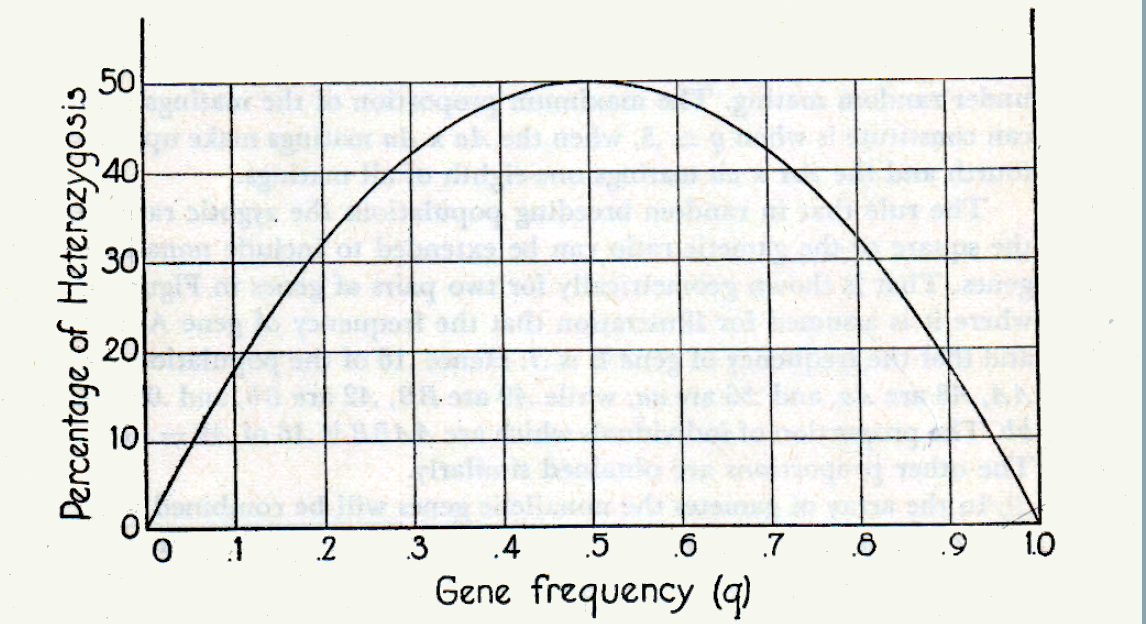
\includegraphics[width=\textwidth]{Figure_3.png}
    \caption{The percentage of heterozygosis as related to gene frequency in a random breeding population.}
    \label{fig:Lush_Figure_3}
\end{figure}

The frequency with which each kind of mating occurs depends much on \textit{q}. Thus, if there are
$q^{2}AA$ males and $q^{2}AA$ females and mating is at random, the most probable proportion of
matings of the type $AA \times AA$ is $q^2 \times q^2$, or $q^4$. Extending this to the other
five types of matings possible, where there are only two alleles, gives the proportions
shown in Figure~\ref{fig:Lush_Figure_4}. Matings of the kinds $AA \times AA$ or $aa \times aa$ can constitute
anything from none to all of the matings in the population according to the value of \textit{q}.
Matings of the kinds $AA \times Aa$ and $AA \times aa$ can constitute from none to 42 per cent
of the matings. The maximum figure is reached for the $AA \times Aa$ mating when \textit{q} = .75
and for the Aa x aa mating when q = .25. Regardless of q, matings of the type $Aa \times Aa$ are
always just twice as frequent as matings of the type $AA \times aa$ under random mating. The maximum
proportion of the matings they can constitute is when \textit{q} = .5, when the $Aa \times Aa$
matings make up one-fourth and the $AA \times aa$ matings one-eighth of all matings.
\index{Heterozygosis|)}

\begin{figure}[htbp]
    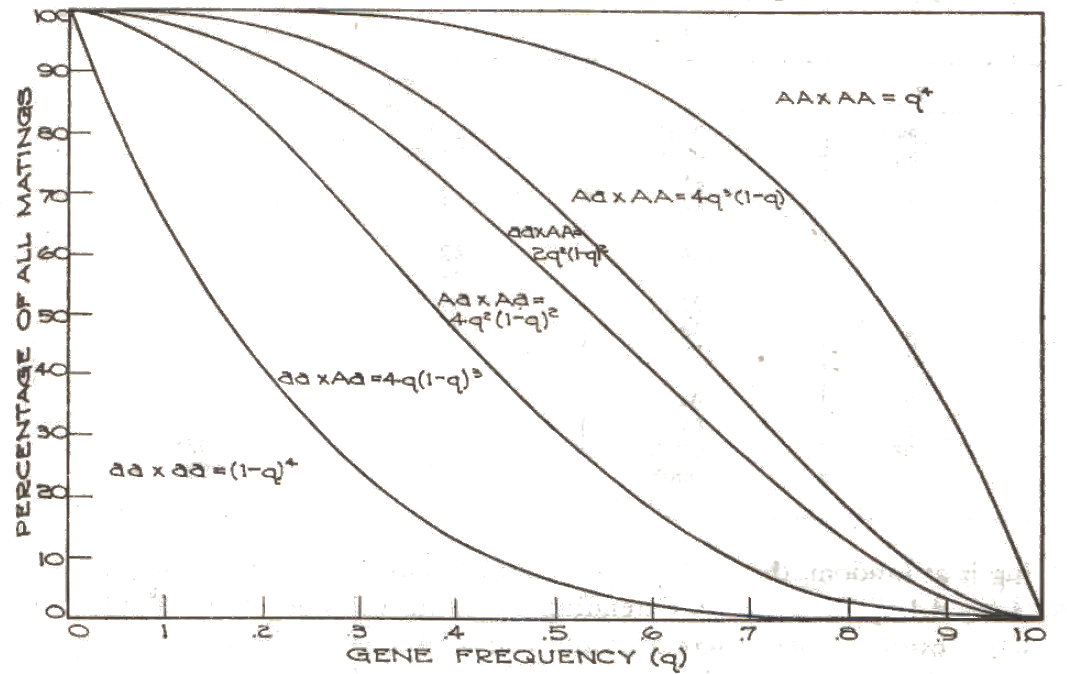
\includegraphics[width=\textwidth]{Figure_4.png}
    \caption[justification=justified]{Showing how the abundance or scarcity of each kind of mating changes with gene frequency in a population mating at random. Vertical distances are in proportion to the frequency of each
    		 kind of mating.}
    \label{fig:Lush_Figure_4}
\end{figure}

The rule that in random breeding populations the zygotic ratio is the square of the gametic ratio can be
extended to include nonallelic genes. That is shown geometrically for two pairs of genes in
Figure~\ref{fig:Lush_Figure_5}, where it is assumed for illustration that the frequency of gene A is .4
and that the frequency of gene B is .7. Hence .16 of the population are \textit{AA}, .48 are \textit{Aa},
and .36 are \textit{aa}; while .49 are \textit{BB}, .42 are \textit{Bb}, and .09 are \textit{bb}. The
proportion of individuals which are \textit{AABB} is .16 of .49 =.0784. The other proportions are obtained
similarly.

\begin{figure}[htbp]
    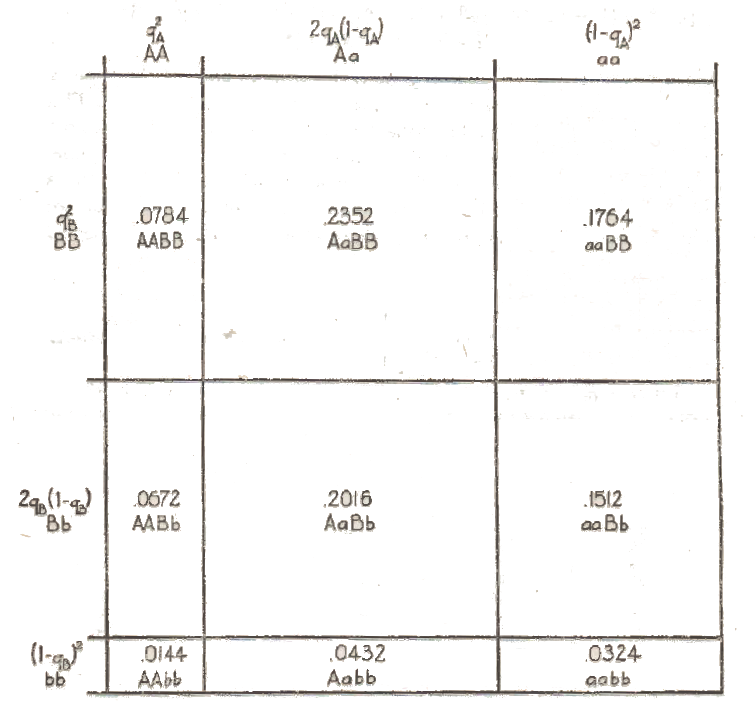
\includegraphics[width=\textwidth]{Figure_5.png}
    \caption{Showing how the rarity or abundance of the various genotypes in a random breeding population
    	     depends on the frequency of the genes in each pair.}
    \label{fig:Lush_Figure_5}
\end{figure}

In the array of gametes the nonallelic genes will be combined with each other independently except under
three circumstances. First, if the population is the result of a recent cross, the
\index{Coupling and repulsion}coupling and the
repulsion phases of linked genes may not yet have had time to become equally abundant. Second, if the
parents were produced by assortive mating (See Chapter 27), genes which produce similar
effects will be together in the same gametes more frequently than otherwise. Third, if the parents are a
selected group (rather than a random sample or a typical sample of their generation), the gametes they
produce will contain slightly fewer extreme combinations and more intermediate combinations than if the
same genes were combined entirely at random.

The two-factor $F_2$ ratio, used in genetics texts to introduce the subject of inheritance where more than
one pair of genes is involved, is only the special case in which the frequency of both genes is exactly .5.
The zygotic ratio when \textit{n} genes combine at random can be had by multiplying all the zygotic ratios
for each pair of genes together thus:

\begin{gather*}
	\left[ q_{A}A + (1-q_{A}a) \right]^2 + \left[ q_{B}B + (1-q_{B}b) \right]^2 +
	\left[ q_{C}C + (1-q_{C}c) \right]^2 + \ldots + \\ \left[ q_{N}N +
	(1-q_{N}n) \right]^2
\end{gather*}

\index{Homozygosis|(}
If the frequency of the desired gene is the same in each of the \textit{n} pairs,
the formula can be written in a simpler form: $[q_A + (1 - q_A)]^{2n}$. This
shows why the search for breeding animals homozygous in all desired genes has no
prospect for immediate success unless the number of genes desired is very small
and the desired gene in each pair already has a high frequency. Table~\ref{tbl:Lush_Table_3}
shows the expectation for various values of \textit{q} and \textit{n}, figures being shown
only where at least 1 in 1,000 is expected to exist.

\begin{center}
	\begin{table}[htbp]
		\caption{\textsc{Portion of Random Bred Population Which Will Be Homozygous For}
		\textit{n} \textsc{Desired Genes =} $q^{2}_{A}q^{2}_{B}q^{2}_{C} \ldots q^{2}_{N}$\\
		Let $q_A = q_B = q_C = \ldots = q_N$. Then portion equals $q^{2n}$}
		\label{tbl:Lush_Table_3}
		\begin{tabular}{C{2cm}|C{2cm}|C{2cm}|C{2cm}|C{2cm}}
			\hline
			\hline
						& \multicolumn{4}{c}{\textit{n}} \\
			\cline{2-5}
			\textit{q}	& 5		& 10		& 20		& 50 \\
 			\hline
			.50			& .001	& \ldots	& \ldots	& \ldots \\
			.60			& .006	& \ldots	& \ldots	& \ldots \\
			.70			& .028	& .001		& \ldots	& \ldots \\
			.80			& .107	& .012		& \ldots	& \ldots \\
			.90			& .349	& .122		& .015		& \ldots \\
			.95			& .599	& .358		& .128		& .006 \\
			.98			& .817	& .668		& .446		& .133 \\
			.99			& .904	& .818		& .669		& .366 \\
 			\hline
		\end{tabular}
	\end{table}
\end{center}

Animals having at least one desirable gene in each pair but not
necessarily homozygous for all those pairs are much more frequent.
Thus, if $q^2$ are \textit{AA} and $2q(1 - q)$ are \textit{Aa}, those
which carry \textit{A} either in the homozygous or in the heterozygous
condition are $q^2 + 2q(l - q)$, which may be written $q(2 - q)$.
Extending this to \textit{n} pairs of genes gives the figures shown in
Table~\ref{tbl:Lush_Table_4}. Animals possessing at least one desired
gene in each pair are more apt to exist in large enough proportions that
it will be finitely possible to find them and to breed from them, discarding
all which do not come up to this standard, than is the case with
animals homozygous for the desired genes.

\begin{table}[htbp]
	\centering
	\caption{\textsc{Portion of Random Bred Population Which Will Possess at Least One
	Desired Gene in Each Pair =} $q_A(2-q_A)q_B(2-q_B)q_C(2-q_C) \ldots q_N(2-q_N)$.\\
	If $q_A = q_B = q_C = \ldots = q_N$, then portion equals $[q{2-q}]^n$}
	\label{tbl:Lush_Table_4}
	\begin{tabular}{C{2cm}|C{2cm}|C{2cm}|C{2cm}|C{2cm}}
		\hline
		\hline
					& \multicolumn{4}{c}{\textit{n}} \\
		\cline{2-5}
		\textit{q}	& 5			& 10		& 20		& 50 \\
 		\hline
		.30			& .035		& .001		& \ldots	& \ldots \\
		.50			& .237		& .056		& .003		& \ldots \\
		.70			& .624		& .389		& .152		& .009 \\
		.80			& .815		& .665		& .442		& .130 \\
		.90			& .951		& .904		& .818		& .605 \\
		.95			& .988		& .975		& .951		& .882 \\
		.99			& .999		& .999		& .998		& .995 \\
 		\hline
	\end{tabular}
\end{table}

In any actual population some of the animals will come nearer than
others to having all the desired genes, even though none of them perhaps
comes close to that ideal. The practical breeder's simplest reasonable
hope is that by selection he can steadily increase the frequency of
the desirable genes until sometime --- perhaps not until after many
generations --- they may reach such a high frequency that perfect breeding
animals may be born in his herd. But whether or not that goal is actually
attained in his lifetime, the increasing frequency of the desired genes
will carry the average merit of the population with it, so that he can
reap the reward for his efforts in each generation in which there actually
is any increase in the frequency of the desirable genes.

In most circumstances the practical breeder is much more interested
in average genetic merit than in homozygosity itself. For example, if
10 pairs of genes affect a trait and a breeder is choosing between one
animal which is homozygous for five of the desired genes but homozygous
for the undesired gene in the other five pairs and another animal
which is \index{Heterozygosis}heterozygous for all 10 pairs, there will be little difference in
their breeding usefulness to him. Each has 10 desired genes. On the
average each will transmit five desired genes to an offspring, the former
to every offspring without exception and the latter sometimes more and
sometimes less than five. Probably the wiser choice would be for the
more heterozygous animal since the greater variability of its offspring
offers more chance for rapid progress by selection among them.
\index{Gametic ratio|)}
\index{Gene frequency|)}
\index{Homozygosis|)}

\section*{DEVIATIONS FROM RANDOM MATING AS THEY AFFECT THE BINOMIAL DISTRIBUTION OF ZYGOTES}

Mating is random when mates are no more and no less like each
other than if they were paired by drawing numbers out of a hat. Random
mating does not mean promiscuity or carelessness. Deviations
from random mating may be of four genetically different kinds: (1)
inbreeding, (2) outbreeding, (3) mating like to like on the basis of
somatic resemblance, and (4) mating individuals which are somatically
unlike each other. There can, of course, be breeding systems which
involve combinations or alternations of two or more of these. Selection,
which is deciding that certain individuals shall have many offspring
while others shall have few or none, may be practiced along with
random mating among those selected to be parents. An illustration is
the breeding practiced on large ranches where sires and dams may be
highly selected to conform to the owner's standards, but after the selections
are made, several sires and many females are turned loose in the
same pasture and the matings within that pasture are random, so far as
concerns any human control over them. This is selection plus random
mating within the group selected to be parents. If the ideals toward
which the selections are made differ on different ranches, mating may
be random within the limits of each ranch but will not be random with
respect to the whole breed, since animals of like types will tend to be on
the same ranch and therefore will mate together more often than would
be the case if all the sires and dams on all the ranches were in one pasture.

Each of these systems of breeding which is not random will be the
subject of a later chapter. Inbreeding tends to make the array of zygotes
more like that which would exist if the array of gametes were changed
into zygotes by doubling all the genes in each gamete. Inbreeding promotes
the formation of families of all kinds, thus adding to the diversity
of the population. Outbreeding, which prevails when mates are less
closely related to each other than if they were mating at random, is the
reverse of inbreeding and cancels many of its effects. It is especially
potent in destroying family differences which have been produced hy
inbreeding, and at producing hybrid vigor or \index{Heterosis}``heterosis.'' Unless distinct
families already exist, outbreeding cannot be carried far. The
general effect of mating like to like, within the whole group of parents
selected to produce the next generation of the breed, is to make the
population more variable by providing more than a random chance for
gametes from an extreme individual to meet with gametes from an individual
which is extreme in the same direction. The mating of unlikes
together makes the population more uniform by making it more likely
that gametes from an extreme individual will unite with gametes from
an individual extreme in the opposite direction than would be the
case under strictly random mating. It is the most potent breeding system
for producing immediate uniformity in a population but produces
nearly all its effects in the first generation practiced. It is practiced
much where the ideal is intermediate and the breeder seeks to mate
them so that each will compensate for the defects of its mate.
\index{Binomial distribution|)}
\index{Random mating|)}
\index{Zygotic ratios|)}

\section*{REFERENCES}

\begin{hangparas}{0.5in}{1}%
Belling, John. 1931. Chromomeres of liliaceous plants. Univ. Calif. Pub. Bot., 16:
153--70.

Cole, L. J., and Jones, Sarah V. H. 1920. The occurrence of red calves in black
breeds of cattle. Wisconsin Agr. Exp. Sta., Bul. 313.

Fisher, R. A. 1930. The genetical theory of natural selection. (See especially pp.
17--18 and 38--41.)

Gowen, John W., and Gay, E. H. 1933. Gene number, kind, and size in Drosophila.
Genetics, 18:1--31.

Ibsen, H. L. 1933. Cattle inheritance. I. Color. Genetics, 18:441--80.

Juli, M. A. 1934. The inheritance of sexual maturity, rate, and persistency of laying
in the domestic fowl. Poultry Science, 13:286--89.

King, H. D. 1932. Mutations in a strain of captive gray Norway rats. Proc. Sixth
Internat. Cong. of Genetics, 2:108--10.

Muller, H. J., and Prokofyeva, A. A. 1935. The individual gene in relation to the
chromomere and the chromosome. Proc. Nat. Acad. Sci., 21: 16--26.

Rhoades, M. M., and McClinLock, Barbara. 1935. The cytogenetics of maize. Botanical
Review, 1:292--325.

Skovsted, A. 1932. Nordisk Jordbrugsforskning, 5:201--5.

Stadler, L. J. 1932. On the genetic nature of induced mutations in plants. Proc.
Sixth Internat. Cong. of Genetics, 1:274--94.

``Student.'' 1934. A calculation of the minimum number of genes in Winter's
selection experiment. Annals of Eugenics, 6(Part 1):77--82.

Sumner, F. B. 1932. Genetic distributional and evolutionary studies of the subspecies
of deer-mice (Peromyscus). Bibliographia Genetica, 9:1-106.

Wriedt, Chr. 1929. Den mendelske spaltning av fettprosenten ved kryssning av r{\o}dt
dansk og jerseyfe. Nordisk Jordbrugsforskning, 103--21.
\end{hangparas}
\chapter{The Genetic Basis of Variation}
\label{cha:genetic-basis-of-variation}
\index{Environment and heredity|(}
\index{Nonadditive interactions of heredity and environment|(}
\index{Variation!genetic basis of|(}

Variation --- differences between individuals --- is the raw material on
which the breeder works. It is not necessary that the animals vary widely
enough that the breeder can at the very start find some perfect ones
to select, but merely that some of them will be closer to his ideal than
others are.

The causes of variation are differences in the heredity with which
individuals started life, and differences in the environments, internal
and external, known and unknown, to which they were exposed during
their development. Except in the case of identical twins\index{Identical twins}, two individuals
rarely if ever start with all their genes identical.\footnote{In organisms
which can reproduce asexually, (as many plants can by cuttings, budding,
etc.,) large groups of individuals with identical heredity can occur. These
are called ``clones.'' A highly inbred line either of plants or animals,
also approaches the condition in which all individuals in it have the same
heredity, but this approach is asymptotic and it is rarely if ever possible
to be sure that complete identity of heredity has been reached. The broad
term, ``isogenic line,''\index{Isogenic lines} which includes identical twins, clones, and
completely inbred lines, is convenient where it is desired only to mean that
all members of the group have identical heredity, regardless of how that
group was produced.} No two individuals ever develop under absolutely
identical environments. Hence in practice an observed difference between two
individuals must always be considered as the net result of some differences
in their heredity and some differences in their environment. Hereditary and
environmental differences may have been far from equal in the size of the
effects they produced, but almost always both will have been present. They may
have opposed each other or both may have worked in the same direction.

Besides these two main divisions of variation into hereditary and
environmental portions, a third portion (necessary for logical completeness)
comes from joint effects of heredity and environment which cannot fairly be
ascribed to either one alone. Such joint effects may occur either if heredity
and environment are correlated or if they interact in some nonadditive way so
that the effect of a particular variation in heredity may be larger in one
environment than in another or, conversely, a certain change in environment
may make a large change in individuals of some genotypes but only a small
change in other individuals whose genotypes make them less labile.

Positive correlation between heredity and environment makes the
whole population more variable by preventing the plus effects of variations
in heredity from being canceled in individual animals by the
minus effects of variations in environment, or vice versa, as often as
would be the case if the two were uncorrelated. Such a correlation is an
ever-present possibility in data which are collected from a variety of
farms, since it often happens that the man who tries hardest to give his
animals the best environment also tries hardest to select the animals
with the best heredity and has some degree of success in both efforts.
Correlation between heredity and environment is also likely to exist in
data concerning the mental and social traits of man, since inherited
aptitudes on the part of the parents tend to cause them to create in their
own homes environments which favor the development of those same
special abilities in their children. These children will also inherit some
of the same genes which made those parents have those aptitudes in the
first place.

It seems likely that the nonadditive combination effects of heredity
and environment are generally small in amount,\footnote{For some extreme
examples, consult Chapter 5 of Hogben's \textit{Nature and Nurture}.}
but some interactions of this kind do occur.
\index{Environment and heredity|)}
\index{Nonadditive interactions of heredity and environment|)}

\section*{MODES OF GENE EXPRESSION}
\index{Additive effects of genes|(}

The simplest way in which the effects of various genes are combined
is that the substitution of a gene for its allel produces a certain plus or
minus shift in the measurement of the characteristic affected and that
this change --- the ``effect'' of that gene substitution --- is the same, regardless
of what other genes are present. As a physical example, consider
how adding or subtracting one more brick makes exactly the same
increase or decrease in the weight of a brick pile, regardless of the number
or kind of bricks the pile already contains. Some genes may combine
their effects exactly in this simple way and many seem to do so to some
extent, yet many genes are known to interact with each other so that the
outward result of substituting a gene for its allel is larger in some genotypes
and smaller or zero or even reversed in other genotypes. Thus the
actual effect of the gene substitution in each separate individual may
depend partly on what other genes are present.

A simple example is \index{Dominance|(}dominance. If dominance exists, the outward
effect of substituting gene \textit{A} for \textit{a} is larger when the
substitution is made in an individual which is \textit{aa} than when it
is made in one which is \textit{Aa}, although the effect on breeding value
of the individual is the same; namely, that it now transmits \textit{A} to
one-half of its offspring which would otherwise have received \textit{a}
from it. Dominance is nonadditive combination of the effects of genes which
are in the same allelic series. When the effect of making two such gene
substitutions in an \textit{aa} individual is not simply twice as large as
the effect of one, some degree of dominance exists.

\index{Epistatic effects|(}
Genes which are not allelic may also modify the magnitude or even the
direction of each other's effects. A classic example is Bateson's case of
white and purple flowers in sweet peas. He found that two different pairs of
genes, both showing dominance, were necessary for the production of the purple
color. Plants which were \textit{cc} had white flowers, no matter whether they
were \textit{RR}, \textit{Rr}, or \textit{rr}; and plants which were \textit{rr}
had white flowers, no matter whether they were \textit{CC}, \textit{Cc}, or
\textit{cc}. But plants which were either \textit{CC} or \textit{Cc} and were also
\textit{RR} or \textit{Rr} had purple flowers. It is as if \textit{R} produced an
enzyme necessary for developing color and \textit{C} produced the substrate on which
the enzyme could work. Whether the substitution of \textit{C} for \textit{c} will
produce a change from white to purple depends on whether \textit{R} is also present,
as well as on whether the substitution is made in a \textit{cc} or in a \textit{Cc}
individual. The difference between purple and white is a joint effect the credit or
blame for which cannot wholly be divided fairly, part to one gene and the rest to the
other. An example in which the direction of the effect depends on other genes is the
case of the \textit{E} gene in guinea pigs, which darkens certain colors in the presence
of the \textit{P} gene but lightens them in \textit{pp} individuals. Many other kinds of
nonadditive combinations of the effects of genes are known. Some common examples are:
inhibiting genes, threshold effects\index{Threshold effects}, and the general class of cases in which the outward
extreme is genetically an intermediate. The latter may be very common among physiologically
complex characteristics where the degree of expression of the characteristic depends on
the harmonious interplay of a number of different organs and processes.

\section*{SUBDIVISION OF HEREDITARY VARIATION}

In an actual population there will be genes acting in all these ways,
and the number of genes and possible kinds of interactions between
them is so enormous that there is no possibility of learning exactly
what each gene does in every combination. The simplest way to think
of this tangled situation is to imagine that one could average the effects
(some of them large, some small, some positive, some negative, etc.)
which a gene substitution actually does have in that particular population
and then proceed as if this \textit{average effect} were the \textit{actual
effect} of that gene substitution in all genotypes and under all environmental
circumstances which occur in that population. In effect this is what we do
when we speak of a gene as ``good'' or ``bad,'' or as ``a gene for high
production.''

By adding these average effects of all the genes which an animal has
we can obtain an ``expected'' value, or measurement of the appearance
or individual performance of this animal. The expected and the actual
characteristics may not be exactly the same, if the genes interact in
nonadditive ways. The expected value of an individual corresponds more
closely to its breeding value than its own appearance or performance
does.

The variation of the expected values from each other is the additively
genetic portion of the actual variation. Differences between the
expected and the actual values are deviations from the simple additive
scheme. It is convenient to divide these nonadditive deviations into two
groups, the first being the deviations caused by dominance and the second
being the nonadditive interactions of genes which are not allelic
to each other. For brevity these latter are called ``epistatic'' deviations
in this book, although this is a broader use of epistatic than Bateson
intended when he introduced the word.

To understand the principles of what we do when we separate the
additively genetic variation from that due to dominance deviations,
consider the two cases shown in Figure~\ref{fig:Lush_Figure_6}. Polled is
considered a simple dominant over horns in cattle.\footnote{This fits most
of the facts as far as yet known, but there are a few sets of data in which
the situation seems more complicated. Also dominance is not always complete,
scurs being some indication of heterozygosis.} The frequencies of the three
genotypes in this example were assumed to be: \textit{PP}, .01; \textit{Pp},
.18; and \textit{pp}, .81. These are not far from the present frequencies of
the three types in the Hereford breed as a whole in the United States.
Probably there actually are slightly more \textit{PP} and fewer \textit{Pp}
individuals than this.

The actual or phenotypic values are indicated by Y's and the expected or
genetic or breeding values are indicated by G's. The G values come nearer
to agreeing with the Y values than could any other three values which lie on
a straight line.\footnote{The \textit{G} values must lie on a straight line
since they are made to conform to the assumption of no dominance; i.e., the
phenotypic change expected from substituting \textit{P} for \textit{p} is to
be the same when the substitution is made in \textit{Pp} individuals as when
it is made in \textit{pp} individuals. The \textit{G} values are completely
determined by the requirement that the sum of the squares of their deviations
from the \textit{Y} values shall be the least possible for any set of three
values which are on a straight line. This is the ``least squares'' method for
fitting a straight line as closely as possible to observations which do not
actually lie on a straight line.} In technical statistical terms, the line
connecting the \textit{G} values shows the regression of phenotypic values on
breeding values. If there were no dominance $Y_{Pp}$ would lie on a straight
line connecting $Y_{pp}$ and $Y_{PP}$ and the \textit{G} values would fit the
\textit{Y} values exactly. Hence the discrepancies between each \textit{G} and
the corresponding \textit{Y} (on the vertical scale) are called dominance
deviations. Vertical differences between the G values are the additively genetic
deviations. If we let the difference between horned and polled be one unit on
the vertical scale, we can compare on a quantitative basis the additively
genetic variation and the dominance deviations and find how important both are.
We get the following values:

\begin{table}[htbp]
	\centering
	\begin{tabular}{lccc}
		Genotype				& \textit{pp}	& \textit{Pp}	& \textit{PP} \\
		Frequency				& $.81$			& $.18$			& $.01$ \\
		Actual phenotype, Y		& $y$			& $y+1.00$		& $y+1.00$ \\
		G value					& $y+.01$		& $y+.91$		& $y+1.81$ \\
		Y--G					& $-.01$		& $.09$			& $-.81$ \\
	\end{tabular}
\end{table}

\noindent
When we summarize the variation in terms of ``variance''\index{Variance|(} {(See
page \pageref{page79}) we find that 18/19 of the actual variation is included in the
variation of the G values, while only 1/19 of it has to be charged against
the dominance deviations. In this case the additive scheme comes near to telling
all the truth, even though dominance is complete. The G values are far apart and
the variation between them is large. The discrepancy between G and Y is very
small for the \textit{pp} genotype which includes most of the individuals. Nearly
all the rest of the individuals are in the \textit{Pp} group where the dominance
deviation is also rather small. The dominance deviation is large for the
\textit{PP} group, but the \textit{PP} animals are rare and hence contribute only
a few deviations to the total and do not have much influence.

\begin{figure}
	\centering
    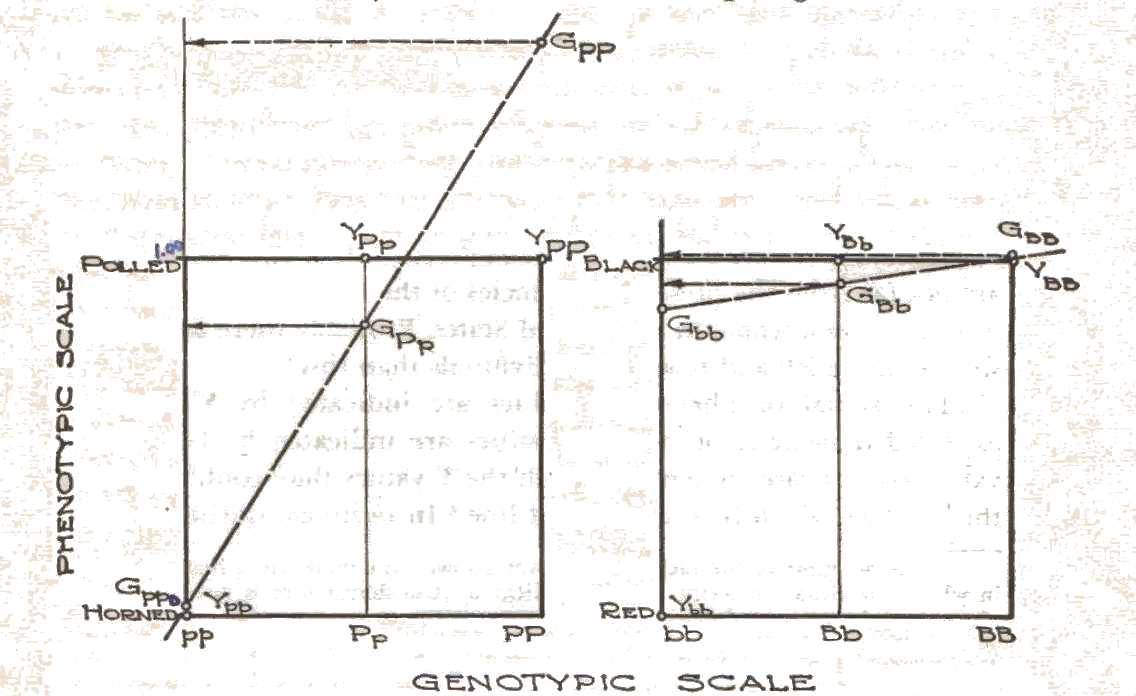
\includegraphics[width=\textwidth]{Figure_6.png}
    \caption{Diagram of regression of phenotype on genotype where only additively
    		 genetic variance and dominance deviations arc involved. Left: A case
    		 where the dominant is rare, the G-values arc far apart, and most of
    		 the variance is additive. Right: A case where the recessive is rare
    		 and the dominance deviations cause much more variance than the
    		 differences between G-values.}
    \label{fig:Lush_Figure_6}
\end{figure}

The average effect of substituting \textit{P} for \textit{p} may be computed as
follows: For every 100 individuals in the population there will be 180 \textit{p}
genes and 20 \textit{P} genes. Of the \textit{p} genes 18 are in \textit{Pp}
individuals where changing them to \textit{P} would produce no phenotypic effect.
The other 162 are in \textit{pp} individuals and for any one of these a change to
\textit{P} would change the phenotype of its possessor one full unit. Hence the
average effect of substituting \textit{P} for \textit{p} in this particular population
would be $\frac{162}{180} = .9$ unit.\footnote{This simple arithmetical way of
computing the average effect illustrates its meaning and will be correct when the
\index{Heterozygosis}heterozygotes are present in the same proportion as they would be under random mating.
When they are more abundant or less abundant than that, the average effect should he
computed by the more technical procedure which is called the least squares method of
fitting a straight line.}

Obviously, the size of the average effect and the comparative importance
of additive and dominance variations will depend on the frequency
of the genotypes, as well as on the degree of dominance. These are
part of the description of this particular population.

The right side of \ref{fig:Lush_Figure_6} shows for comparison how different the
situation is when the recessive is very rare. The \textit{Bb} pair of genes
determines the contrast between black and red in cattle, black being completely
dominant. The frequencies assumed for the genotypes are about what they would be
in black breeds of cattle in which one calf in each 200 is born red. The actual
variation is small and the variation between the G values accounts for on1y
$\frac{14}{107}$ of it. Dominance deviations account for the rest, $\frac{93}{107}$.
The contrast between the left and the right sides of \ref{fig:Lush_Figure_6}
illustrates the general fact (of which more in \textbf{\textit{Chapter 11}}) that
dominance is an \textit{important} source of confusion or hindrance to progress by selection
only when the undesired recessive is already rare. Even when dominance is complete,
the variance among the G values will account for $\frac{2(1-q)}{2-q}$ of the actual
variance\label{page79} in random breeding populations, \textit{q} being the frequency of the
dominant gene.
\index{Variance|)}

For a numerical example of epistatic variance, let us take again the
case of purple and white flowers in sweet peas. Its genetic basis is definite
and well-known, and it is generally considered to be a rather
extreme case of epistasis -- although that idea may need revision when
we learn more about the usual results of making several gene substitutions
at one time. If the sweet peas were breeding at random,\footnote{The sweet pea does
not really fulfill this condition, since it is largely self-fertilizing.} and if the
frequencies of the \textit{C} gene and of the \textit{R} gene were each .5, then
the various genotypes would occur in the proportions shown in column 1 of
Table~\ref{tbl:Lush_Table_5}.

\begin{table}[htbp]
	\centering
	\caption{\textsc{Illustration of the Basis for Separating Additive Genetic Variations, From
			 Deviations Caused by Dominance and Epistasis, Using Bateson's Case of Purple
			 and White Color in Sweet Peas}}
	\label{tbl:Lush_Table_5}
	\begin{tabular}{C{2cm}|C{2cm}|C{1.25cm}|C{2cm}|C{2.25cm}}
		\hline
		\hline
					& & \multicolumn{3}{C{6cm}}{Values on a Scale on Which White = 0 and Purple = 1} \\
		\cline{3-5}
		Frequency With Which the Various Genotypes Would Occur	& Fraction of the \textit{e} Genes of the Whole Population Which Are in This Genotype & Actual	& ``Expected''	& Deviations Due to Dominance and Epistasis \\
 		\hline
		1 ccrr	& $1/8$	& 0	& $-3/16$	& $+3/16$ \\
		2 Ccrr	& $2/8$	& 0	& $+3/16$	& $-3/16$ \\  
		2 ccRr	& $2/8$	& 0	& $+3/16$	& $-3/16$ \\
		1 CCrr	& none	& 0	& $+9/15$	& $-9/16$ \\
		1 ccRR	& $1/8$	& 0	& $+9/16$	& $-9/16$ \\
		4 CcRr	& $2/8$	& 1	& $+9/16$	& $+7/16$ \\
		2 CcRR	& $1/8$	& 1	& $+15/16$	& $+1/16$ \\
		2 CCRr	& none	& 1	& $+15/16$	& $+1/16$ \\
		1 CCRR	& none	& 1	& $+21/16$	& $-5/16$ \\
 		\hline
	\end{tabular}
\end{table}

If we let the difference between purple and white be one unit on the scale on which
we measure color, then in this population the average effect of substituting
\textit{C} for \textit{c} is $3/8$ of a unit. That may be computed as follows:
One-half of all the \textit{c} genes are in \textit{Cc} individuals (the second,
sixth, and seventh lines in Table~\ref{tbl:Lush_Table_5}), where, on account of
dominance, the substitution would make no change in the color. One-eighth of the
\textit{c} genes are in \textit{ccrr} individuals (the first line in
Table~\ref{tbl:Lush_Table_5}), where the substitution would produce no outward effect
because the \textit{R} gene, which is also necessary for the production of purple, is
not present. The remaining three-eighth of the \textit{c} genes are in \textit{ccRR}
or \textit{ccRr} individuals, where the substitution of \textit{C} for \textit{c}
would produce the full change from white to purple. One unit of change in three-eighths
of the cases plus no change in five-eighths of the cases makes an average effect of
three-eighths of a unit for substituting \textit{C} for \textit{c} in that population,
although the actual change would not be exactly three-eighths of a unit in any one
plant.\footnote{For a more detailed discussion of this conception of the average effect of a
gene substitution, see the first few pages of Wright's article beginning on p. 243 of
volume 30 of the \textit{Jour. of Genetics}, or pages 53--56 in volume 11 of
\textit{Annals of Eugenics}, 1941.} The expected values shown in Table~\ref{tbl:Lush_Table_5}
were found by the additional requirement that the average of the expected values must
be the same as the average of the actual values. Figure 7 shows graphically how near the
actual and the ``expected'' values are to each other. The differences between them (the last
column in Table~\ref{tbl:Lush_Table_5}) are the deviations caused jointly by dominance and
epistasis.

\begin{figure}
	\centering
    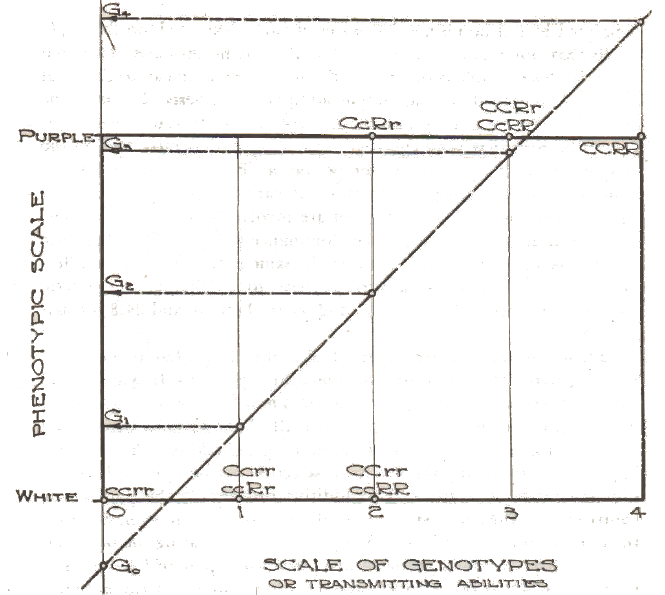
\includegraphics[width=\textwidth]{Figure_7.png}
    \caption{Regression of phenotypes on transmitting ability in a case involving epistatic
			 deviations in addition to dominance deviations and additive differences.
			 $G_0 \cdots G_4$ are the expected values or transmitting abilities of
			 individuals which have $0, 1, \cdots, 4$; respectively, of the \textit{C}
			 and \textit{R} genes. Differences (on the vertical scale) between the
			\textit{G} values are the additive variation. Differences (on the vertical
			scale) between each \textit{G} value and the corresponding actual value are
			deviations caused by dominance and epistasis together.}
    \label{fig:Lush_Figure_7}
\end{figure}

\index{Variance|(}
Variance due to dominance and variance due to epistasis can be
separated by setting up another series of values expected, on the hypothesis
that dominance is complete but there is no epistasis. The final
result in this example is that $4/7$ of the actual variation can be gathered
into and described by the simple additive hypothesis, $2/7$ must be
charged to dominance deviations, and only $1/7$ to epistatic deviations.
It will be seen that the expected values are partly determined by the
frequencies with which the genotypes occur. They are partial descriptions
of a particular population and may vary from one population to
another, even where the same genes are involved. The relative importance
of additive genetic variance, dominance deviations, and epistatic
deviations will change also. Thus, in the same example but with different
gene frequencies the ratio of additive to dominance to epistatic
variance becomes 12:9:2 when $q_R$ and $q_0$ are both .6, and 24:8:9 when
both are .4.

These illustrations are intended to make clear what is meant by
dividing hereditary variation into these three portions. In actual practice
the breeder or investigator will not know exactly what genes are
present, nor the frequency of each, nor all of the ways in which they
interact with each other. Rough estimates of the additive variance can
be had from observing the results of selection or the likeness between
different kinds of relatives. The additive variation is the part which
contributes in the simplest and most direct way to the likeness between
relatives. Knowledge of its size is important for estimating the probable
results of any proposed breeding plan. For many practical purposes it
may not be worth while to separate the dominance and the epistatic
portions from each other.

The additive genetic variation caused by a gene can become zero
only when the average effect of that gene is zero; that is, when the sum
of all the plus changes which it causes is exactly equal to the sum of all
the minus changes which it causes in other genotypes in that same
population. Most of the variation which a gene causes will be included
in the additive portion if its average effect is large. For most of its variation
to be epistatic requires that its average effect be near zero but that
it produce large plus effects in some genotypes and correspondingly
large minus effects in other genotypes. As yet there are only a few actual
data to indicate whether epistatic variations are abundant and important,
or so rare and small that ignoring them in practice would not
cause many errors.\index{Additive effects of genes|)}
\index{Dominance|)}
\index{Epistatic effects|)}

\section*{THE MEASUREMENT OF VARIATION}
\index{Variation!measurement of}

The methods of measuring variation are inconveniently technical for those not
trained in statistical methods. Moreover, there are several of them, and each
has advantages for certain purposes. For reasons which do not concern us here,
the importance of various causes in producing the variability of a population is
most conveniently expressed in terms of the ``variance'' ($\sigma^2$) of that
population. The variance may be defined as the average of the squared deviations
of the individuals from the population average.\footnote{Since the known average
of the \textit{n} individuals in the sample studied may not be exactly the same as
the unknown average of the much larger population from which the sample comes, the
sum of the \textit{n} squared deviations of individuals from the average of the
sample is divided by $n - 1$ instead of \textit{n} to obtain the best estimate of
the variance of the population.} An equivalent definition is that the variance is
one-half of the average squared difference between pairs of individuals chosen at
random. The square root of the variance is called the ``standard deviation''\index{Standard deviation}
($\sigma$), which, since it is expressed in the same terms as the original
measurements, is often more convenient for expressing the variations of individual
items than is the variance, which is expressed in squares of the original
measurements. In a ``normally distributed'' population about two-thirds of the
individuals differ from the average by less than the standard deviation, while
about one-sixth of the individuals will be more than one standard deviation above
the average. The remaining sixth will be below the average by more than one standard
deviation. Only about one-fortieth of the individuals will be more than twice the
standard deviation above the average and another fortieth will be more than twice
the standard deviation below the average. In small populations the standard
deviation is usually about one-fourth to one-sixth of the difference between the
largest and the smallest individuals (the ``range''); but that rule is not very
accurate, since the range depends on only two individuals and is subject to large
sampling errors. The arithmetic average of the deviations, neglecting signs, is
about .8 as large as $\sigma$, but for various reasons is not as dependable and is almost
never used.
\index{Variance|)}

\index{Normal distributions|(}
Not all populations are ``normally'' distributed, although most of
those encountered in breeding practice are nearly enough so that the
statistics of the normal curve may be used with little error for practical
purposes. The normal curve is frequently called the ``Gaussian curve''
after the mathematician who first studied it in detail, or the ``curve of
error'' because its first application, which is still its principal application
in some sciences, was in making allowance for unavoidable but
random errors of observation. It is symmetrical and bell-shaped, as will
be seen in Figure~\ref{fig:Lush_Figure_8}.

\begin{figure}
    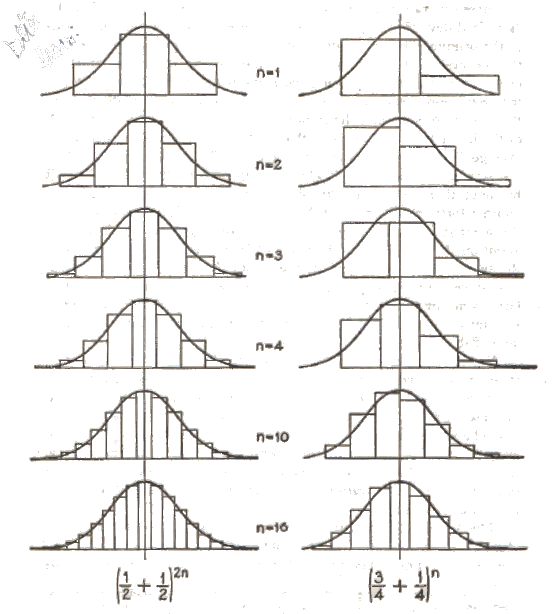
\includegraphics[width=\textwidth]{Figure_8.png}
    \caption{Binomial distributions for \textit{n} pairs of genes with equal effects
    		 and superposed normal curves with equal mean, equal area, and equal
    		 variance. Left: No dominance. Right: Complete dominance in the same
    		 direction in all pairs of genes.}
    \label{fig:Lush_Figure_8}
\end{figure}

\index{Binomial distribution|(}
The statistical cornerstone for the genetics of populations is the
``binomial distribution,'' which is obtained by expanding the expression
$(a + b)^n$. This is just the mathematical description of what results
naturally from the duplicateness of inheritance and the ``one-or-otherness''
of gene transmission; that is, of Mendel's laws of segregation and
recombination. \index{Dominance|(}The Mendelian mechanism guarantees that in a random-
mating\index{Random mating|(} population the zygotes\index{Zygotic ratios|(} will be distributed according to the
square of the gametic ratio. The genotypes for characteristics determined
by \textit{n} pairs of genes\index{Variation!as affected by gene numbers} with equal frequencies and equal effects will
have the binomial distribution corresponding to $[qA + (1 - q)a]^{2n}$.
If the gene frequencies are not the same for all pairs of genes, the
distribution will be somewhat less variable than if they were all equal but
had the same average. If the different pairs of genes do not have equal
effects, the distribution of the genotypes is more variable than if the
same number of genes each played equal parts in producing the same
total effect. When $a = b$ (or $q = 1 - q$ in the genetic formula) and
\textit{n} is large, the binomial distribution approaches the normal
distribution so closely that for practical purposes they may be treated alike,
especially in small populations. The binomial curve can be distinctly skewed
to one side if all of the genes which operate in the plus direction happen
to be much more frequent than their alleles, or the reverse . It can also be
skewed if the genes multiply each other's effects instead of combining additively,
or if there are threshold or other epistatic interactions.
Figure~\ref{fig:Lush_Figure_8} shows on the left side several symmetrical
binomial curves with normal curves superposed on them. With some additional
environmental modifications to blur the accuracy of classification, the binomial
curve, even with very small values of n, could not be surely distinguished from
the normal curve in small populations. The right side of Figure 8 shows how the
skewness produced by dominance, even when the dominance is all in one direction,
is extreme when \textit{n} is small butwould be difficult to detect in small
populations if there were as many as 10 pairs of genes involve d, especially if
there were also many variations from environmental causes.
\index{Binomial distribution|)}
\index{Dominance|)}
\index{Normal distributions|)}

\index{``Blending inheritance''|(}
\index{Variance|(}
\index{Variation!maintained by Mendelian mechanism|(}
One of the most important consequences of the Mendelian mechanism of inheritance
is that it maintains the variability of an interbreeding opulation at a nearly
constant level over long periods of time, thus aintaining a supply of variability
available for selection or other reeding practices. The importance of this may be
shown most clearly y contrasting it with what would be expected under the blending
theory of inheritance. Under that theory, if the sire deviated \textit{x} and the
dam deviated \textit{y} from the mean of the race, \textit{every} offspring from
that mating would be expected to deviate $\frac{x + y}{2}$ The average squared
deviation (the variance) of the parents would be $\frac{x^2 + y^2}{2}$. The average
squared deviation of the offspring would be $\frac{x^2 + 2xy + y^2}{4}$. If the
parents mated at random, sires with positive values of \textit{x} having no especial
tendency to mate with dams which had positive values of \textit{y}, the term
\textit{2xy} would be zero (since the negative terms would cancel the positive
ones); and the average squared deviation of each generation would be \textit{only
half as large as that of the preceding one}. The group would thus  approach perfect
uniformity at a tremendous rate. Even a pronounced tendency for like to mate with
like would delay this approach only a little (by causing \textit{2xy} to have a
positive value) unless the tendency of like to mate with like were perfect.
Figure~\ref{fig:Lush_Figure_9} shows how rapidly the hereditary variability
existing at any one time would be ``swamped'' if inheritance really were blending,
and how much of the hereditary variability existing at any one moment must have
come from mutations which had just occurred in the last few generations, if the
variability of a population were to remain the same from generation to generation.
Much of the skepticism about Darwin's theory of evolution by natural selection had
its roots in the tacit assumption that inheritance is ``blending'' and the consequent
belief that selection would have to be almost instant and perfect in its seizure of
new variations if these were to be incorporated into the species before they were
lost. In the older view, heredity was a conserving force and variation was contradictory
to it. That is now obsolete as it is seen that the mechanism of heredity conserves
individual variation also. Knowledge of Mendelism and of the hereditary variation to be
expected between full brothers has freed us from the supposed necessity of thinking that
mutations are frequent or important in practical breeding problems. It has also relieved
us from the necessity of believing that selection must act almost at once if it is to
utilize variations before they are ``swamped'' or lost. In many respects Mendelism has
rounded out the Darwinian theory of the power of natural selection by showing that some
of its us supposed weaknesses do not exist.\footnote{See pp. 1--12 of Fisher's
\textit{The Genetical Theory of Natural Selection}.}

\begin{figure}
    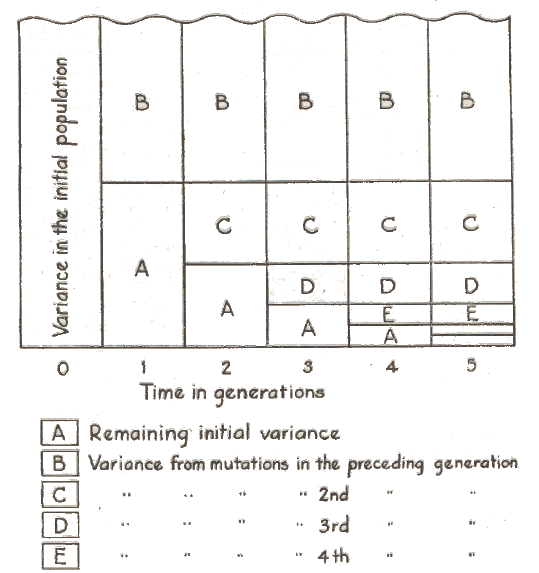
\includegraphics[width=\textwidth]{Figure_9.png}
    \caption{Rate at which initial hereditary variance was supposed to be lost and the
			 supposed recent origin of the hereditary variations existing at any one time,
			 according to the former theory that inheritance really blended.}
    \label{fig:Lush_Figure_9}
    \index{Random mating|)}
    \index{Variance|)}
\end{figure}

Mendelism gives us a picture of a stable population composed of
changing individuals, or of endless individual variations which added
together result in an almost constant population. A Mendelian population
may be compared to a group of bees around a hive. Almost every
bee is constantly in motion and yet the average position of the swarm
may remain almost the same hour after hour. The individuals are
dynamic -- the population is almost static. Changing a population by
selection may be compared roughly to driving a herd of many hundred
steers. At any one time there are steers moving in all possible directions,
yet the drivers, by constantly discouraging those which attempt to move
toward the rear and leaving the road open to those which go in the
desired direction, can succeed in moving the herd a few miles each day.
\index{``Blending inheritance''|)}
\index{Variation!maintained by Mendelian mechanism|)}
\index{Zygotic ratios|)}

The \textit{Correlation coefficient|(} is a measure of how closely two things
tend to vary in the same direction. Examples are the tendency in human
data for father and son both to be tall or both to be short and the tendency
for tall men to weigh more than short men. In both cases the
tendency is pronounced enough that it is a matter of common knowledge,
even to those who have never heard it expressed quantitatively. In
both cases there are frequent and striking exceptions. In the former
case the measurements are the same kind (i.e., stature), and they are
paired together on account of the genetic relationship of their possessors.
In the latter case the measurements (i.e., stature and weight) are
different in kind and are paired together because they apply to the same
individual. The general idea of correlation is simple and universally
understood, but the coefficient for measuring degrees of correlation is
technical enough that considerable practice in computing it on
various kinds of data is usually necessary for proficiency in understanding
it. The coefficient of correlation is expressed on a scale running
from $+1.0$, where two characteristics vary in perfect step with each
other, through zero, where there is no correspondence at all, to $-1.0$,
where there is a perfect tendency to vary in exactly opposite directions
from each other.

\index{Regression|(}
\textit{Regression} is the general statistical term for expressing how much
one variable may be expected to change per unit change in some other
variable. As a concrete example, in dairy cattle regression of daughter's
fat yield on dam's fat yield is the average amount of increase in the fat
production of the daughter which we may expect for each extra unit of
fat the dam produced. Historically regression gets its name from acertain
aspect of correlation wherein it was observed that the offspring of
extreme parents are usually nearer to the average of the population
than their parents were; i.e., they regress toward the mean of the race.
This idea of regression of the offspring from the parents toward the
mean of the race was later extended to all kinds of equations for predicting
one variable from another, where the relation between the two
is not perfect. Regression is now used in many cases which do not
involve questions of heredity at all and even in cases where the idea of
the correlation coefficient would be artificial, as in time trends. The customary
symbol for the correlation coefficient, r, was originally chosen
because it was the first letter of the word regression. Thus, it is a
reminder of the once intimate relation between the two ideas!

\section*{SUMMARY}

Variation is the raw material with which the breeder works. For
purposes of subdivision into its constituent parts, variation is best measured
in terms of ``variance,'' which is the average squared deviation of
the individuals from the population average. According to its causes,
variance may be divided into three main parts: that due to variations in
environment ($\sigma_E^2$), that due to differences in heredity ($\sigma_H^2$), and that
due to joint effects of variations in heredity and environment ($\sigma_{HE}^2$)
which are nonadditive or othenvise intertangled so that they cannot
fairly be ascribed to heredity or to environment alone. The hereditary
variance may be further subdivided into three portions: the additive
genetic variance, which includes all that can be described by assuming
that the effects of the whole combination of genes in the individual
equal the sum of the average effects of those genes ($\sigma_G^2$); the variance
caused by dominance deviations from the additive scheme ($\sigma_D^2$); and
the variance caused by epistatic deviations from the additive scheme
($\sigma_I^2$).

For expressing the variation of individuals, or for expressing differences
between expected and actual values, variation is most conveniently
expressed in the form of the standard deviation ($\sigma$), which is the
square root of the variance. In most populations about two-thirds of
the individuals differ from the population average by less than the
standard deviation.

The tendency for two different characteristics of the same individual,
or for the same characteristic in pairs of individuals related in a certain
way, to vary in the same direction is measured by the ``coefficient
of correlation.'' The equation for predicting the value of one characteristic
which will most probably correspond with a given value of
another characteristic is called a ``regression'' equation.
\index{Correlation coefficient|)}
\index{Regression|)}
\index{Variation!genetic basis of|)}
\index{Variation!measurement of|)}
\chapter{Heredity and Environment}
\label{cha:heredity-and-environment}
\index{Environment and heredity|(}
\index{Heritability|(}

In the strictest sense of the word, the question of whether a characteristic
is hereditary or environmental has no meaning. Every characteristic
is both hereditary and environmental, since it is the end result of a
long chain of interactions of the genes with each other, with the environment
and with the intermediate products at each stage of development.
The genes cannot develop the characteristic unless they have the
proper environment, and no amount of attention to the environment
will cause the characteristic to develop unless the necessary genes are
present. If either the genes or the environment are changed, the characteristic
which results from their interactions may be changed.

Nevertheless, it is often convenient to speak of a characteristic as
``hereditary'' or ``highly hereditary'' when we wish to emphasize that
most of the differences we usually see between individuals in that characteristic
are caused by differences in the genes they have, and only a
few of the differences between individuals are caused by differences in
the environments under which they developed. The difference between
black and red coat color in cattle is such an example of a highly hereditary
characteristic. Environmental circumstances, such as exposure to
sunshine, may cause the black to vary from a jet black to a rusty or
brownish black: but that is a tiny variation compared with the large
difference between black and red which is caused by differences in
genes.

With equal logic it is often convenient to call a characteristic ``environmental''
or ``only slightly hereditary'' when most of the differences
ordinarily found between individuals in that population are caused by
differences in the environments under which they developed and only
a small part of those differences between individuals are caused by differences
in the genes they have. Examples of such largely environmental
characteristics are degrees of fatness and of lameness. In most
populations variations in those are much more apt to have resulted
from previous management, feeding, accidents, or condition of general
health than from differences in heredity. Yet it is certain that some
individuals have genes which make them fatten more readily than others, or
have genes causing structural weaknesses which predispose them to
lameness.

The whole matter of whether a characteristic is hereditary or environmental,
if we find it convenient to state it in that way, is a question
of how much of the variation in that characteristic in that population is
caused by differences in heredity and how much is caused by differences
in environment.

\index{Variance|(}
The question of whether heredity or environment is the more
important can be phrased precisely for a particular trait in a particular
population and, if the data are available, can be answered. It does not
have a single answer true for all traits in one population nor for the
same trait in all populations. Let $\sigma_O^2 =$ the actually observed variance,
$\sigma_H^2 =$ that part of the variance caused by differences in the heredity
which different individuals have, and $\sigma_E^2 =$ that part of the variance
caused by differences in the environments under which different individuals
developed. Then\footnote{In order not to confuse the argument, the nonadditive
interactions of heredity and environment are neglected here. There is reason to
think that those joint effects will generally be small. This definition includes
as ``hereditary'' the dominance and epistatic deviations since they result from
differences between whole genotypes, although they will not contribute so much to
the likeness between relatives as the additive differences do.} $\sigma_H^2 +
\sigma_E^2 = \sigma_O^2$ and $\frac{\sigma_H^2}{\sigma_H^2 + \sigma_E^2} =
\frac{\sigma_H^2}{\sigma_O^2} =$ the portion of the observed variance for which
differences in heredity are responsible. When this fraction is large, we say
that the characteristic is highly hereditary; when this fraction is small, we
call the characteristic slightly hereditary or largely environmental.

The value of $\frac{\sigma_H^2}{\sigma_H^2 + \sigma_E^2}$ can be altered by
changing either $\sigma_H^2$ or $\sigma_E^2$. If we try to make the environment
exactly the same for all individuals, as is usually attempted in genetic experiments,
we may go far in that direction although we can hardly hope to control the environment
perfectly. So far as we succeed in making $\sigma_E^2$ smaller than it is in the
general population, we make the variations in that characteristic more
highly hereditary in our material than they were in the general population.
If we also enlarge $\sigma_H^2$ in our material by mating like to like while
selecting for opposite extremes or by inbreeding in several separate
lines, we increase $\sigma_H^2$ and make variations in that characteristic in our
material still more highly hereditary. Unless we are quite aware of what
we have done in partially controlling the environment (and thus making
$\sigma_E^2$ tend toward zero) and in selecting or breeding to increase the
genetic diversity of our laboratory material, we are apt to get an
exaggerated idea of the importance of heredity in causing variations in that
characteristic in the general population. On the other hand, if we are
experimenting with the effects of some procedure in nutrition or in
management, we will probably try to make $\sigma_H^2$ as small as possible by
using a uniform stock, discarding at the beginning of the experiment
any which appear to deviate much in either direction from the population
average, and minimizing the hereditary differences between lots by
putting litter mates in different lots, etc. Then we will also make our
experimental (environmental) treatments so contrasting that we will be
reasonably sure to find differences in their results. Again, unless we are
quite aware of what we did in neutralizing hereditary differences and in
magnifying environmental differences in our laboratory material, we
are apt to get an exaggerated idea of how important our environmental
differences are in causing the variations in the general population. If
this were clearly understood, a considerable amount of fruitless controversy
would be avoided.

A quantitative statement of the relative importance of heredity and
environment is a partial description of the causes of the variation in a
particular characteristic in the specified population. It is useful in estimating
the probable results of certain breeding systems in the next
generation or two, but it tells nothing about the ultimate limits of the
changes which might be made in that population either by breeding or
by altering its environment.

\section*{METHODS OF ESTIMATING HERITABILITY}
\index{Heritability!methods of estimating|(}

All methods of estimating heritability rest on measuring how much
more closely animals with similar genotypes resemble each other than
less closely related animals do. The techniques suitable for doing this
vary with the material and according to whether environmental correlations
between relatives and the peculiarities of the mating system, if it
was other than random, can be measured and discounted by other
means.

Variation within isogenic lines is wholly environmental. Comparing
this with the variation in an otherwise similar random breeding population
may give an estimate of heritability. This method is of little use in
farm animals because among them are no isogenic lines\index{Isogenic lines} except occasional
pairs of identical twins. These are difficult to identify but if
sought diligently and studied intensively might finally give reliable
information. Identical twins\index{Identical twins} are to be compared with ordinary twins,
rather than with pairs of individuals unrelated to each other, lest the
similarities in the environments of twins might lead to errors in the
interpretation. The method of isogenic lines is the only method likely
to measure all of the epistatic and dominance variations as well as the
additive ones but, because of the rarity of identical twins\index{Identical twins} in farm animals,
is not promising as a source of information fairly free from
sampling errors.

In selection experiments, if we can measure the amount by which
those selected to be the parents exceeded the average of their generation,
we can divide that into the amount by which the average of the
offspring exceeded the average of the generation in which their parents
were born. This gives a measure of the additive portion of the variance
plus a portion (somewhat less than half) of the epistatic variance. In
order not to be misled by unnoticed environmental changes, it is usually
necessary that selection be practiced in opposite directions at the
same time, so that the interpretation will be based on differences
between the high and the low lines, rather than on the absolute values
of the averages. Sometimes this method can be followed in experiments
especially designed for this purpose at some research institution, but it
is not often available to the breeder, since he can rarely afford to select
in the undesired direction just to get information on heritability.

The resemblance between parent and offspring is the most widely
useful method, but is likely to include some environmental correlation
between parent and offspring. Also it will include something from the
resemblance of the offspring to the other parent, if mating were not
random. In using this method the procedure is as follows: (1) observe
the correlation between parent and offspring, (2) subtract from that the
environmental contribution, (3) double the remainder, and (4) divide
by one plus the correlation between mates.\footnote{This should be the
genetic correlation (coefficient of relationship) if the departures
from random mating were of the inbreeding kind, but should be the actually
observed correlation if the mating choices were based on each animal's own
individuality for the characteristic being studied. One will rarely be
certain about this.} The second step is always likely to be difficult,
and the fourth will be unless the deviations from random mating are known
more exactly than is usually the case.

A useful dodge which makes steps two and four unnecessary is to
divide the mates of each sire into a high and a low half on their own
performance, combine the data for all sires, divide the difference
between the daughters of the high and the low halves by the difference
between the two groups of dams and double the results. This measures
the additive portion and a bit of the epistatic portion of the differences
between such dams as were mated to the same sire. It leaves unanalyzed
the differences between the groups of cows which get mated to different
sires. A similar division of the offspring of the high and low sires mated
to the same dam would answer as well in principle but, because of the
usually small number of offspring per dam, is rarely possible with farm
animals.

One of the first clearly analyzed cases of the relative importance of
heredity and environment was Wright's study of the amount of white
spotting in a stock of guinea pigs. It will illustrate the principles and
the use of nearly isogenic lines and of correlation between relatives.
Besides the control stock, in which even second cousin matings had
been avoided, there was a stock which came from the same foundation
but which had been inbred full brother and sister for more than 10
years (probably about 20 to 25 generations in most branches of the family,
nearly all of which came from a single mating in the twelfth generation),
so that it must have been almost entirely homozygous and could
have retained but little genetic variability. By measuring the average
likeness between parents, between parents and offspring, and between
litter mates, Wright was able to separate the variance into a portion
due to heredity, a portion due to environment common to litter mates,
and a remainder due to environment or embryological accidents which
were not alike even for litter mates. Table~\ref{tbl:Lush_Table_6} shows
the findings. The
most illuminating fact for our present purpose is that the variance due
to environment was almost the same in actual units of measurements.
(.354 and .372) in both stocks but was 97.2 per cent of the variance in
inbred stock and only 57.8 per cent of the variance in the control stock.
Here is a case where the same characteristic in two separate stocks
derived from the same colony by different breeding methods is very
slightly hereditary (2.8 per cent) within the inbred stock and nearly
half (42.2 per cent) hereditary within the control stock. All that really
happened was that in one stock the inbreeding had caused nearly all of
the initial hereditary variability to be lost and thereby had altered
greatly the proportion of hereditary to environmental variability.

\begin{table}[htbp]
	\centering
	\caption{\textsc{Piebald Spotting in Guinea Pigs. Portions of the Variance According to Causes
			 (After Wright)}}
	\label{tbl:Lush_Table_6}
	\begin{tabular}{L{3cm}|C{1.5cm}|C{1.5cm}|C{1.5cm}|C{1.5cm}}
		\hline
		\hline
					& \multicolumn{2}{C{3.5cm}|}{$\sigma^2$ in the Inbred Stock}	& \multicolumn{2}{C{3.5cm}}{$\sigma^2$ in the Control Stock} \\
		\cline{2-5}
		Causes of Variance						& Actual Units	& Percentage of Total	& Actual Units	& Percentage of Total \\
 		\hline
		Heredity								& .010			& 2.8					& .271			& 42.4 \\
		Environment common to litter mates		& .020			& 5.5					& .002			& .3 \\
		Environment not common to litter mates	& .334			& 91.7					& .370			& 57.5 \\
		\hline
		Total									& .364			& 100.0					& .643			& 100.0 \\
		\hline
	\end{tabular}
\end{table}

The following are some examples of the kind of analysis which can
be made by comparing correlations between relatives. Gowen studied
Jersey Register of Merit data on milk yield and fat percentage, assuming
that there was no correlation between the environments of daughter
and dam. He came to the conclusion that about 50 to 70 per cent of
the variance in milk production and about 75 to 85 per cent of the
variance in fat percentage came from variations in the heredity of the
individual cows. But if there was as much as .10 to .20 of environmental
correlation betwen [\textit{sic}] daughter and dam, as seems probable from the
usually observed correlation between the records of herd mates, these
figures are too high by .20 to .40. Plum's analysis of the records of cows
in Iowa Cow Testing Associations led him to the figures shown in
Table~\ref{tbl:Lush_Table_7}. Studies of intrasire regression of daughter on dam have
generally given values of around .15 to .30 for heritability of differences in
fat production between cows in the same herd where each cow was
represented by only one record.
\index{Heritability!methods of estimating|)}

\begin{table}[htbp]
	\centering
	\caption{\textsc{Relative Importance of Causes of Variation in Butterfat Production}}
	\label{tbl:Lush_Table_7}
	\begin{tabular}{L{7cm}|L{2cm}L{2cm}}
		\hline
		\hline
		Causes of variation	& \multicolumn{2}{C{4cm}}{Percentage of Total Variance} \\
 		\hline
		Breed											&					& 2 	\\
		Herd											&					&   	\\
		\tabindent Feeding policy of herd				& 12				&		\\
		\tabindent Other causes (genetic or environmental)	& \underline{21}	&		\\
														&					&		\\
														&					& 33	\\
		Cow (mostly genetic)							&					& 26	\\
		Residual (year to year variations)				& 					&		\\
		\tabindent Feeding variations within the herd	& 6					&		\\
		\tabindent Other year to year differences		& 1					&		\\
		\tabindent Length of dry period					& 1					&		\\
		\tabindent Season of calving					& 3					&		\\
		\tabindent Other factors						& \underline{28}	&		\\
														&					& 39	\\
		\hline
		Total											&					& 100	\\
		\hline
	\end{tabular}
\end{table}

Lush, Hetzer, and Culbertson, studying the birth weights of pigs
born during 15 years at the Iowa Agricultural Experiment Station,
came to the figures shown in Table~\ref{tbl:Lush_Table_8}. Part of the 29
per cent due to ``other'' environment common to litter mates may really
have been hereditary as the result of hereditary differences among the dams,
although it was environmental as far as the pigs themselves were concerned.
There is much evidence that the dam's own size or other characteristics
have much influence on the birth weights of her offspring.

\begin{table}[htbp]
	\centering
	\caption{\textsc{Relative Importance of Causes of Variance in Birth Weights of Pigs}}
	\label{tbl:Lush_Table_8}
	\begin{tabular}{L{7cm}|L{2cm}L{2cm}}
		\hline
		\hline
		Causes of variance	& \multicolumn{2}{C{4cm}}{Percentage} \\
 		\hline
		Heredity of the pigs						&					& 	 	\\
		\tabindent Breed differences				& 2					&		\\
		\tabindent Sex								& 1					&		\\
		\tabindent General							& \underline{3}		&		\\
													&					& 6		\\
		Environment common to litter mates			&					&   	\\
		\tabindent Litter size						& 7					&		\\
		\tabindent Year								& 5					&		\\
		\tabindent Ration							& 4					&		\\
		\tabindent Gestation length					& 2					&		\\
		\tabindent Other							& \underline{29}	&		\\
													&					& 47	\\
		Environment not common to litter mates		&					& 47	\\
		\hline
		Total										&					& 100	\\
		\hline
	\end{tabular}
\end{table}

The figures in Tables~\ref{tbl:Lush_Table_7} and \ref{tbl:Lush_Table_8}
illustrate how the actual data may permit subdividing the environmental
variance into portions caused by certain tangible factors or groups of
factors. Nearly always a considerable part of the variance will remain
unidentified as to causes. These are most naturally inferred to have been
individual unobserved (or at least unrecorded) variations in environment,
but in some cases may really have been errors in observations or (in some
methods of analysis) will also have included those portions of the epistatic
or dominance variations which did not contribute to the likeness of the
relatives studied. For other examples similar to Tables~\ref{tbl:Lush_Table_6}
to \ref{tbl:Lush_Table_8}, yet each showing some special features of its own,
see: \textit{Genetics} 19:535; 21:360; 22:468; 26:217; 31:503; and
\textit{Onderstepoort Jour. Vet. Sci. and An. Husb.} 5:580.
\index{Variance|)}

While it is true that the animal at birth contains all the heredity it is
going to have but has not yet been affected by many of the environ mental
circumstances which will affect it, yet the presence or absence of
differences at birth is not a good criterion of whether those differences
are hereditary. Some of the differences found at birth are the result of
previous differences in intra-uterine environment, or of what for lack
of a better term may be called embryological accidents. On the other
hand, many genes in which individuals may differ do not produce their
effects until the individual reaches a certain stage of development.
Examples are the genes which affect early maturity, milk. production,
shape and quality of teeth, and in man such specific things as baldness,
prematurely gray hair, and Huntington's chorea.

\section*{PRACTICAL APPLICATIONS}

Much individual variation is left even when either the heredity or
environment is perfectly controlled. For example, if half of the variance
in a characteristic is hereditary and half is environmental, perfect
control of heredity would still leave the standard deviation 71 per cent
(the square root of one-half) as large as before. If all environmental
variations in a characteristic which is 80 per cent hereditary were eliminated,
the standard deviation would still be nearly 90 per cent (the
square root of 80 per cent) as large as before. If the hereditary variations
were entirely eliminated, the standard deviation would still be about 45
per cent as large as before. Even if a characteristic were 99 per cent
hereditary, complete elimination of all hereditary variability would
still leave the standard deviation 10 per cent as large as it was originally.
Only those variations which are caused by differences in heredity
are themselves inherited. Variations caused by environment can be
large and very important economically, but they do not change the
inheritance of the animal and are not transmitted to its offspring but
must be produced afresh in those offspring by repeating the environmental
treatments which produced them in the parent. There is not
space here to repeat the proofs for the noninheritance of environmental
effects; and, as with other negative concepts, it may be impossible to
prove this one rigorously. But the many experiments carefully planned
to test whether the effects of environmental treatments are inherited in
such a way that the offspring inherit some degree of the modifications
originally produced in their parents by the environmental treatment
have all given negative or doubtful results. Even one who deliberately
wishes to believe that environment does affect heredity in this way must
admit that the effects are so slight that they are not practically important
in any one generation.\footnote{Certain extreme environments, such as exposure
to X-rays, or to barely sub lethal temperatures, or to radium, do increase
the mutation rate} Perhaps they do not occur at all. Both in improving the
heredity and in improving the environment of his animals the breeder is likely
to encounter the law of diminishing returns. Yet in improving their heredity
there is the possibility that if he can achieve enough -- for example, get his
herd widely known as one of the three or four best sources of breeding stock
in the whole breed -- he may come again to a zone of increasing returns because
of the high prices he will receive. The competition to get into that zone is
usually very strong, however.

\index{Acquired characters, noninheritance of|(}Improvements in heredity are
permanent\footnote{Except for gains in the
epistatic effects. Those tend to disappear as the genes
recombine. One must keep on selecting to hold them.} and each generation
stands on the shoulders of the preceding one, whereas improvements in
the environment produce almost their full effect on the animals for
which they are first made. Each new generation must again receive the
improved environment or the gain will be lost. Hence, in the long run
it may be profitable to spend considerable effort to make small improvements
in heredity, since the expense of making such improvements in
one generation may yield dividends for many generations. The expense
of making improvements in heredity (so far as those are additive) is a
capital investment; the expense of making improvements in environment
is an operating expense. Naturally the breeder will wish to do
both so far as they are profitable.\index{Acquired characters, noninheritance of|)}

Besides the economic value of its direct effects on the animals, environment
needs the practical breeder's attention in two ways; First, the
animals should be kept in an environment which will permit them to
show readily which of them come nearest to having all the genes which
have effects the breeder wishes. Second, the breeder should observe
carefully the environment which applies to each animal so that he can
allow for this when making his selections. It is usually impossible to disentangle
the effects of environment completely from the effects of heredity
in individual cases, but some effort spent in trying to do that will
often do much to make selections more accurate and progress more
rapid.

Breeding animals should be kept under environment like that for
which their offspring are being bred. If animals are being bred for
resistance to unfavorable conditions, they should be kept under unfavorable
conditions so that the breeder will have a chance to learn which
ones have the genes that will make them most nearly what he
wants.\footnote{This reaches its extreme form in breeding for disease resistance, a practice to
which is now devoted a large portion of the efforts in plant breeding, but which is
still in the laboratory stage in animal breeding except where (as, for example, in
the tropics or in the breeds of sheep native to marshy regions) some effective natural
selection has been practiced automatically. For fewest mistakes when breeding for
disease resistance, the exposure or inoculation dose should be severe enough that
somewhere between 30 and 70 per cent of the animals would contract the disease.
That may not be practical for diseases which have a high mortality. Those which
cause only a low mortality may not be important enough to warrant much effort in
breeding for disease resistance. Animal breeders now look first of all for prevention,
vaccines, or medicaments as a more economical way out. But if those fail and we are
driven to breed for disease resistance, the above considerations show how far we will
have to depart from the (at present) more orthodox practices of sanitation and
efforts to prevent exposure.} If
cows are being bred for specialized and intensive dairying, they should
be well fed and milked three times a day, provided those are the conditions
under which commercial cows are to be kept in the specialized
dairying of the future. To feed them poorly or milk them only twice a
day would prevent some of the genes, useful under the more specialized
conditions, from showing their presence. On the other hand, to force
the cows by extravagant feeding and by such extreme practices as milking
four times a day would magnify the differences between their production
records and to that extent would be a help in selecting animals
adapted to these conditions; but for most practical purposes this gain
would probably be more than offset by the fact that some of the cows
would respond more than others to those forced conditions, without
there being a corresponding increase in what they would produce under
the usual conditions for which they are being bred. The breeder of
dual-purpose cattle will make fewer mistakes in his selections if his
breeding cows are tested under twice-a-day milking and other management
like that under which he expects their descendants to be used.

The question of testing under forced conditions or under ordinary
conditions can perhaps be clarified by an analogy. If an athletic coach
were to examine all the men in a college to find the best runners for his
track team and were to test them in a race of only one length, such as a
two-mile race, it is true that most of those who did well in this long race
would also do better than average in the short races; yet there would
certainly be some who had not the endurance for the long race but
could do well in the 100-yard dash. There would be others who could
win in the long race but have not the bursts of speed necessary to make
them good performers in the short races. In brief, each man has a certain
amount of general ability to run, and that will manifest itself in
races of all lengths; but each individual also has certain special abilities
or disabilities which will help him or hinder him in certain lengths of
races but not in others. In order to find the very best runners for each
kind of race the coach will need to test them in that kind of race. Yet if
the correlation between their abilities at one length of race and at others
is high, perhaps he might conveniently eliminate half or more of the
whole group from further consideration, by trying them on one kind of
race, without much risk of losing a runner who would be really outstanding
at some of the other lengths of races. Likewise with farm animals
there is doubtless much correlation between an animal's ability to
do well under many different environments, but that correlation is far
from perfect. The genes which enable it to do well or poorly in a certain
environment will manifest themselves most clearly only when the animal
is kept under that environment. In the writings about race horses
there is much mention of ``stayers'' and ``sprinters,'' indicating that
many horses are good in one of these respects but not in the other. Also
they sometimes speak of ``mudders'' which can do well on a wet track
but are outclassed by many others when the track is dry.

If a breeder can foresee that general conditions of management are
going to change in a certain way in the future, it is of course to his
advantage to change his conditions of testing now, so that, when the
general change comes, his animals will already have been selected for a
generation or two toward adaptability to those conditions. In doing so,
of course, he runs the risk that his prediction of the coming change may
be wrong. If it is, his stock may be changed farther away from the real
goal of the future than if he had made no attempt to foresee a change.

Also, a high record made under forced testing has considerable
advertising value. Not all of the potential customers will discount this
high record as much as they should for the environmental circumstances
under which it was made. While this may even be a hindrance
to breed improvement, yet in some cases it has a commercial value to
the individual breeder which he cannot afford to ignore.

Mistaking the effects of the environment for the effects of genes dulls
the keenness of selections, makes the breeder sometimes save animals he
would cull if he knew what genes they had and sometimes cull animals
which have better genes than most of those he saves. This source of
error is very important for such things as growth rate, fertility, health,
vigor in general, size of fleshy parts, ability to fatten, etc., which are
economically important and physiologically complex and often much
modified by environment. The most important practical consequence is
a regression\index{Regression} of the offspring toward the mean of the race. That is, the
offspring of parents which are extreme in either direction will not
usually average as extreme as their parents. The simplest quantitative
expression for this is that for each unit which the selected parents average
above the mean of their race, their offspring will most probably average
about $\frac{\sigma_H^2}{\sigma_H^2 + \sigma_E^2}$ as far above. This would
be literally true if the genes all combined their effects additively. In
actual fact there will be some dominance and some nonadditive gene
interactions which will produce more regression toward the mean of the
race than this formula shows.\footnote{The formula would be more nearly
correct if the numerator were only the additive genetic portion of the
variance; but that is a slight understatement of the case, since a portion
of the epistatic variance also belongs in the numerator.} Mistaking the
effects of environment for the effects of genes, next to matters of health
and fertility in some species, is usually the biggest obstacle to the
breeder's rapid progress toward his chosen goal.

The remedy for confusing the effects of enviroment with those of
heredity is either to control the environment physically by eliminating
variations in it, testing all animals under standard conditions and thus
reducing $\sigma_E^2$ toward zero, or to control the enviroment
statistically by using correction\index{Standardizing records|(} factors to allow as best
one can for unusual individual circumstances when judging what each animal
would have been under standard environmental conditions or what the
difference between two individuals would have been if they had been under
the same environments.
\index{Standardizing records|)}

Physical standardization of the enviroment can never be perfect.
Partial control may be too expensive to carry far. Statistical control
may actually introduce errors through use of the wrong correction factors.
Yet so far as one makes allowances or corrections which are more
often right than they are wrong, he will eliminate more of $\sigma_E^2$ than of
$\sigma_H^2$. Therefore a larger fraction of the variance in his corrected or
adjusted estimates will be hereditary than was true of the variance in
the original observations. S quch allowances for differences in environmental
conditions may vary from the vaguest kind of a mental allowance
to intricate correction factors which sometimes approach the limit
where the increases they make in the accuracy of selections do not pay
for the labor of making the corrections. The man who sees his animals
every day has an important advantage over the man who does not work
with them himself and sees them only at rare intervals or knows them
only through the report of his herdsman, since the former knows the
environmental differences better and can make fairer allowance for
them. The man who works with his animals daily is, however, more
likely to make too much allowance for his favorites without being aware
that he is doing so.

That the offspring of extreme parent~ generally are nearer to the
average of the breed than their parents were (especially as concerns
characteristics of low heritability), does not automatically make the
breed become more uniform as time passes. The offspring from each
parent will vary among themselves and environment will shove some of
them far up and others far down. The extreme ones thus produced will
replenish the supply of extreme individuals in the next generation.

In medical writings a distinction used sometimes to be made
between ``hereditary'' and \index{``Familial''}``familial,'' the former referring to cases
where the offspring was obviously like one parent, and the latter to
traits (such as recessives or those with low ``penetrance''\index{Penetrance}) which ``run in
families'' but in which the individual might not resemble either parent.
Progress in genetic knowledge has now made that distinction obsolete.

``Hereditary'' in the broad sense of the word has nothing to do with
abundance or scarcity of a characteristic or with dominance, although
some methods of estimating heritability do not gather up the variance
due to dominance deviations. Black is no more and no less hereditary
than the much rarer red in black breeds of cattle; rather the question of
heritability concerns the cause of the contrast, black versus red.

\section*{SUMMARY}

\begin{enumerate}
\item All characteristics are both hereditary and environmental in the
strictest sense of those words.
\item Characteristics called hereditary for convenience are those for
which most of the usual differences between individuals are caused by
differences in the genes those individuals have.
\item Characteristics called environmental or nonhereditary are those
for which most of the differences between individuals result from differences
in the environments to which the individuals were exposed.
\item The effects of environment are not inherited except as extreme
environments (like heavy X-ray radiation) produce mutations, and
those are not adaptively related to the environment which produced
them.
\item The breeder should keep his animals under the environments in
which they and their descendants are intended to be used so that the
desired genes may have a chance to express their effects and be recognized
for selection.
\item The breeder will often mistake the effects of environment for
those of genes and will thus make mistakes in his selections. Such mistakes
are usually the most important cause of the fact that the offspring
of selected extreme parents average nearer than their parents to the
mean of their race.
\end{enumerate}
\index{Environment and heredity|)}
\index{Heritability|)}

\section*{REFERENCES}

\begin{hangparas}{0.5in}{1}%
Gowen, John W. 1934. The influence of inheritance and environment on the milk
production and butterfat percentage of Jersey cattle. Jour. Agr. Res. 49:
433--65.

Jennings, H. S. 1930. The biological basis of human nature. 384 pp. New York:
W. W. Norton \& Co. (See especially pp. 127--37, 203--17 and 218--21.)

Lenz, F. 1939. Was bedeutet ``Erblich'' und ``Nicbt-erblich'' beim Menschen? Proc.
Seventh Intern. Cong. of Genet. pp. 187--90. Cambridge.

Lush, Jay L. 1940. Intra-sire correlations or regressions of offspring on dam as a
method of estimating heritability of characteristics. Proc. Amer. Soc. An.
Prod. 293--301.

---; Hetzer, H. O.; and Culbertson, C. C. 1934. Factors affecting birth
weights of swine. Genetics, 19:329--43.

Plum, Mogens. 1935. Causes of differences in butterfat production of cows in Iowa
cow testing associations. Jour. of Dairy Sci., 18:8ll--25.

Wright, Sewall. 1920. The relative importance of heredity and environment in
determining the piebald pattern of guinea pigs. Proc. of the Nat. Acad.
of Sci., 6:320--32.
\end{hangparas}
\chapter[The Nature of Differences Between Breeds]{The Nature of Differences Between Breeds (or Races or Species or Other Groups) Averages}
\label{cha:differences-between-group-averages}
\index{Breed differences|(}
\index{Variation!of averages|(}

Averages vary less than the individual items on which they are
based. This happens because the items averaged together are not all
alike and their variations partly cancel each other. The average of a
sample of \textit{n} individuals will differ from the average of the population
from which it came by one \textit{n}th of the sum of the individual deviations
which did not happen to be canceled. If the sample is selected at random,
that difference will be small, especially if the sample is large. The
variance of the averages of such random samples is one nth as large as
the variance of individuals. But, if the sample is selected by some method
which tended more often than not to choose individuals with plus
(or with minus) deviations, those individual deviations will be prevailingly
in the same direction and will not cancel each other completely.
Instead, the sample average will tend to be different from the population
average by an amount determined by the method of selection. In
such a case the variation within the sample will be less than if it had
been selected at random.

As a numerical example we may take annual butterfat production,
for which the standard deviation among cows in Iowa cow testing associations
is not far from 100 pounds. We are not much surprised if we
choose two cows at random and find that their records differ by as much
as 100 pounds. In fact, nearly half of all such pairs would differ by that
much or more. But we would be surprised if the average of two groups
of 10 cows, each selected entirely at random, differed by as much as 100
pounds. We would not expect that to happen oftener than once in
about 20 or 25 such comparisons. If it did happen, we would wonder
whether the two groups really had come from the same population or
whether they had been selected in some biased way which tended to
bring higher records into one group and lower ones into the other. If
the one set had all been selected from one herd and the other set had all
come from another herd, we would not be so surprised by that big a
difference, since good or poor management or breeding in either herd
would tend to shove all the records from that herd up or all down
together. In choosing only two herds at random it might easily happen
that we would get one herd with poor management and another with
good management; while, if each record came from a different herd, it
is not at all likely that the IO in one set would all come from well-managed
or well-bred herds and the IO in the other set would all come from
poor herds, unless there was some difference in the method of choosing
the records for each set.

\begin{figure}
	\centering
    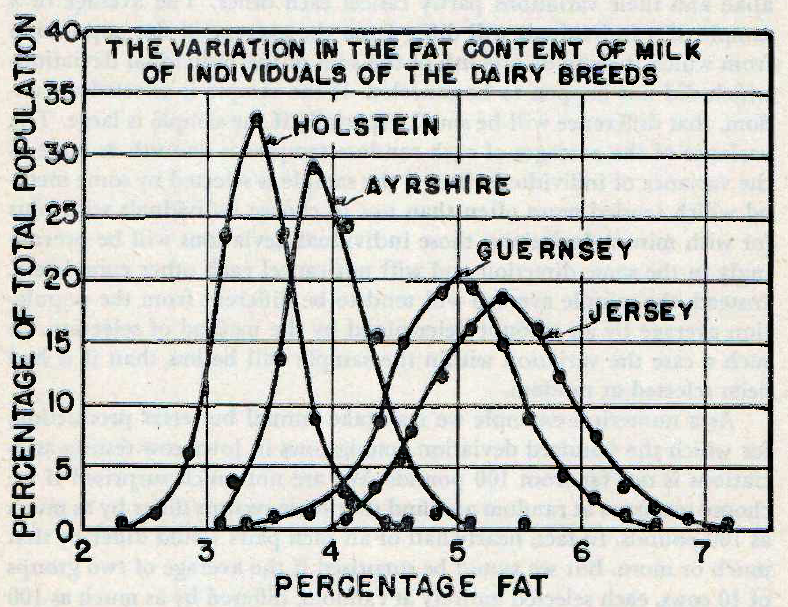
\includegraphics[width=\textwidth]{Figure_10.png}
    \caption{Distributions of individual cows in four dairy breeds according to the
			 percentage of butterfat in their milk. The breeds overlap, but the differences between
			 their averages are real. (Adapted from Bul. 365 of the Mo. Agr. Exp. Station.)}
    \label{fig:Lush_Figure_10}
\end{figure}

Because averages are less variable, it is often possible to be sure that
there is a real difference between two groups which have averages not
very different and in which the individuals vary so widely that the two
groups overlap in much of their range. This is the general situation for
most breed differences, especially for differences in economically important
and physiologically complex characteristics like milk production,
fertility, size or shape of muscular parts, etc. Figure~\ref{fig:Lush_Figure_10} shows this for
percentage of fat in the milk of four breeds of dairy cattle. For some
characteristics, notably color or details of bone dimensions or conformation,
there may be no overlapping at all between breeds. Figure~\ref{fig:Lush_Figure_11}
illustrates graphically the relation between individual differences and
group differences. The fairly common saying, ``There is more difference
within breeds than there is between breeds,'' is often true in the sense
that the difference between the breed averages is small compared with
many of the differences between individuals which belong to the same
breed. This saying is quite misleading, however, if it is interpreted to
mean that the differences between breeds are not real after all. Group
differences of the same kind as are illustrated in Figure~\ref{fig:Lush_Figure_11} often prevail
between races and may prevail between families or other groups
within a breed.

\begin{figure}
	\centering
    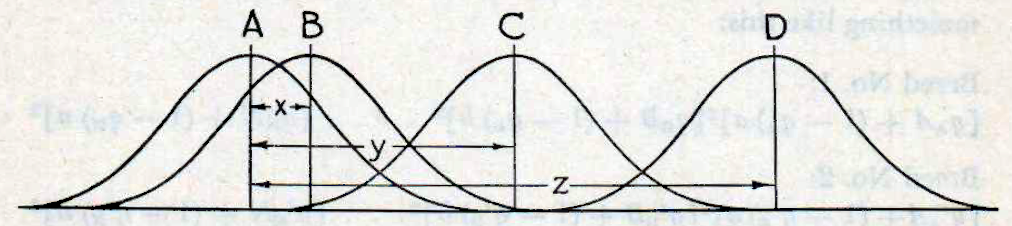
\includegraphics[width=\textwidth]{Figure_11.png}
    \caption{Overlapping frequency curves showing the nature of differences between
			population averages and differences between individuals. \textit{x} is
			the difference between the averages of populations \textit{A} and
			\textit{B}, which overlap in most of their ranges. \textit{y} is the
			difference between the averages of populations \textit{A} and
			\textit{C}, which overlap only a little. \textit{z} is the difference
			between the averages of populations \textit{A} and \textit{D}, which do
			not overlap at all. If two individuals are chosen at random from one
			population. The difference between those two will be larger than
			\textit{x} in far more than half of such pairs and in a few pairs will
			be larger than \textit{y}.}
    \label{fig:Lush_Figure_11}
\end{figure}

It is to be expected that breeds which have been kept separate from
each other in their ancestry for many generations will usually have
drifted apart in many of their characteristics on account of the sampling
variations of Mendelian inheritance in small populations, or will have
been drawn apart by selection which has not been equally successful in
both breeds or has not been directed toward exactly the same ideals.
Breed differences may often be so small that they are economically
unimportant, especially if the breeds have been selected toward almost
the same ideals; yet it would be a remarkable coincidence if the breed
averages were exactly the same for any characteristic. Even where two
breeds have been selected toward the same ideal and their phenotypic
averages are almost the same, the sets of genes by which that phenotype
is produced are likely to have become qualitatively different if the two
breeds have been kept entirely from any crossing with each other for
tens of generations.
\index{Variation!of averages|)}

\index{Homozygosis}
The genetic basis of differences between breeds may be of two kinds.
In the first place, one breed may be homozygous for one gene and
another breed may be homozygous for an allel of that gene. If that were
true for all genes\\index{Variation!as affected by gene numbers|(}\index{Zygotic ratios|(}, we could write the Mendelian formulas of two breeds
as follows:

\begin{table}[htbp]
	\centering
	\begin{tabular}{L{2.5cm}L{2.5cm}L{2.5cm}}
		Breed No. 1		& \textit{AABBccddEE}	&	\textit{NN}	\\
		Breed No. 2		& \textit{aabbCCddEE}	&	\textit{nn}	\\
	\end{tabular}
\end{table}

\noindent
This would indicate that the two breeds are homozygous for different
genes in the series for \textit{A}, for \textit{B}, £or \textit{C} and
for \textit{N}, but are alike in the series for \textit{d} and for
\textit{E}. This conception of breed differences appears to have
been rather widely held by those who discussed the possible practical
applications of Mendelism in the early years of genetics, but it is
expressed less frequently now, as the evidence accumulates that few
genes are homozygous in all members of the breed. The other kind of
genetic situation which may be the basis for distinct breed differences is
that a pair of genes is not entirely homozygous in either breed but the
proportion of one gene to its allel may be widely different in the two
breeds. \index{Gene frequency|(}The Mendelian formulas for the two breeds could be written
something like this:

\begin{table}[htbp]
	\centering
	\begin{tabular}{l}
		Breed No. 1		\\
		$[q_AA + (1-q_A)a]^2[q_BB + (1-q_B)b]^2 \cdots [q_NN + (1-q_N)n]^2$ \\
		\\
		Breed No. 2 \\
		$[q'_AA + (1-q'_A)a]^2[q'_BB + (1-q'_B)b]^2 \cdots [q'_NN + (1-q'_N)n]^2$ \\
	\end{tabular}
\end{table}

\noindent
The blood groups in the Guernsey and Holstein-Friesian breeds of cattle
are a good example of this very situation (\textit{Jour. Ani. Sci.} 3:315--321.
1944). In an extreme case of this sort, such as is illustrated in Figure 12,
two breeds might be alike in the sense that every kind of gene which
exists in the one also exists in the other, and yet be distinctly different
outwardly and in average genotype. Genetic differences of both kinds
probably exist between most breeds. Really, the first kind of difference
is only an extreme limit of the second where \textit{q} = 1.0 in one breed and
is zero in the other.

A complete description of a breed involves not only a statement of the genes
for which it is homozygous and different from other breeds but also a statement
of the frequencies in it of genes for which it is not homozygous and which other
breeds may also possess in larger or smaller frequencies. Thus, a complete
description of a black breed of cattle may contain, besides the statement that
the ``type'' (the most frequent kind) is black, the statement that in this breed
the frequency of gene \textit{B} is .93 and of \textit{b} is .07. Perhaps in
another black breed the frequency of \textit{B} may be .97 or perhaps only .80,
while in a breed like the Shorthorn, where solid black is unknown, the frequency
of \textit{B} is .00. Perhaps other alleles in this series may yet be found.
For example, the genetic explanation of the black pigment present in fawn or
brindle breeds or of such dark pigment as occasionally appears around the eyes
or muzzles of Shorthorns is still uncertain. If such other alleles are found, a
complete description of some other breed may include the statement that in it the
frequency of \textit{B} is .40, of $B_1$ is .45, and of \textit{b} is .15. Naturally
it will be difficult to get such complete information except for a few genes which
individually have conspicuous effects. For a long time to come it is likely that
the practical description of a breed will consist mainly of its averages, or
``type'' in traits which do not lend themselves readily to numerical averaging, with
a few sketchy semi-quantitative comments about its variability in those features.
\index{Gene frequency|)}

\begin{figure}
	\centering
    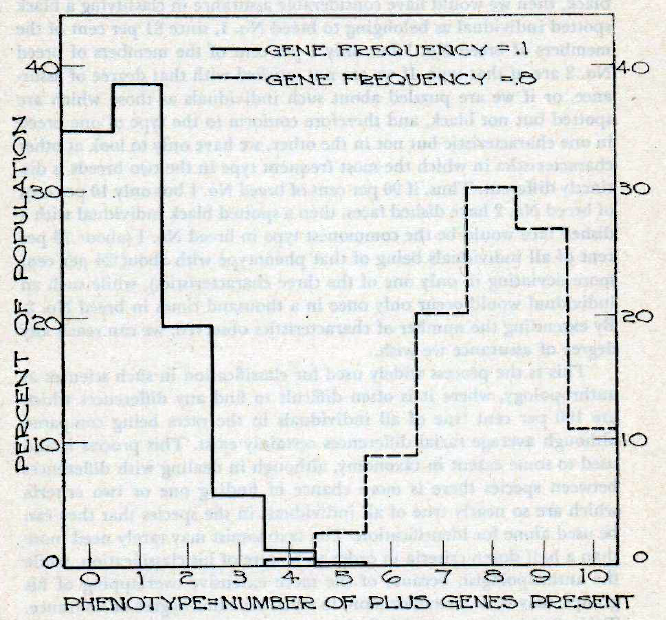
\includegraphics[width=\textwidth]{Figure_12.png}
    \caption{The distribution of genotypes expected in two random breeding populations
			 each of which is heterozygous for five pairs of genes with equal effects. The
			 genes lack dominance and combine their effects additively. In one population the
			 frequency of the plus gene in each of the five pairs is .1, while in the other it is .8.
			 This will illustrate how two breeds could both have exactly the same kinds of genes
			 and yet overlap so little that there would be practically no mistakes in classifying
			 individuals.}
    \label{fig:Lush_Figure_12}
\end{figure}

Two breeds may overlap in every observable characteristic, and yet
it may be possible to identify with certainty the breed to which every
individual belongs. If 90 per cent of the individuals in breed No. 1 but
only 10 per cent of those in breed No. 2 are spotted, we cannot with
much assurance classify the breed of an individual by examining it for
spotting alone. There are too many exceptions to the ``type.'' But if 90
per cent of the individuals in breed No. 1 are black in their colored
areas, while only 10 per cent of the individuals in breed No. 2 are
black, then we would have considerable assurance in classifying a black
spotted individual as belonging to breed No. l, since 81 per cent of the
members of breed No. 1 but only 1 per cent of the members of breed
No. 2 are of that type. If we are not satisfied with that degree of assurance,
or if we are puzzled about such individuals as those which are
spotted but not black, and therefore conform to the type of one breed
in one characteristic but not in the other, we have only to look at other
characteristics in which the most frequent type in the two breeds is distinctly
different. Thus, if 90 per cent of breed No. 1 but only 10 per cent
of breed No. 2 have dished faces, then a spotted black individual with a
dished face would be the commonest type in breed No. 1 (about 73 per
cent of all individuals being of that phenotype with about 24 per cent
more deviating in only one of the three characteristics), while such an
individual would occur only once in a thousand times in breed No. 2.
By extending the number of characteristics observed, we can reach any
degree of assurance we wish.

This is the process widely used for classification in such sciences as
anthropology, where it is often difficult to find any differences which
are 100 per cent true of all individuals in the races being compared
although average racial differences certainly exist. This process is also
used to some extent in taxonomy, although in dealing with differences
between species there is more chance of finding one or two criteria
which are so nearly true of all individuals in the species that they can
be used alone for identification. The taxonomist may rarely need more
than a half dozen criteria in order to be sure of his classification, while
the anthropologist, because of the more extensive overlapping of his
groups, may need a score or more to reach the same degree of assurance.
Table~\ref{tbl:Lush_Table_9} shows in some detail the average number of
\index{Deviations from type|(} deviations from
``type'' which may be expected per individual in a population where
\textit{n} independent characteristics are being examined and in each of those
characteristics \textit{t} is the fraction of individuals which deviate from type.
The average number of deviations expected in an individual is \textit{nt}. The
figures which follow the $\pm$ signs are standard deviations computed by
the formula, $\sigma = \sqrt{nt(1 - t)}$, which must be interpreted with
reservation on account of the distinct skewness of the distribution where \textit{t} is
far from .5. The standard deviations show that, when the average number
of deviations from type is large, there may be no individuals which
are exactly like the ``type.'' For example, when \textit{n} = 20 and \textit{t} = .40, the
average individual will deviate from ``type'' in 8 respects, only about
one-eighth of them will deviate from type in as few as 5 respects, only 1
in 20 in as few as 4 respects. Less than I in 27,000 will conform exactly
to type in all 20 respects. In this sense it may be true that in finite populations
there is \textit{no such thing as an average individual}, but that does not
impair the usefulness of the average for describing the group. The
description of the group will be more complete if something is also
stated about the variation to be expected in each characteristic.

\begin{table}
	\centering
	\caption{\textsc{Average Number of Characteristics per Individual Expected to Deviate From
			 the ``Type'' of the Group Where} \textit{n} \textsc{Characteristics are Observed
			 and} \textit{t} \textsc{is the Fraction of Individuals Which Deviate From Type in
			 Each Respect}}
	\label{tbl:Lush_Table_9}
	\begin{tabular}{L{2cm}|C{3cm}|C{3cm}|C{3cm}}
		\hline
		\hline
					& \multicolumn{3}{c}{\textit{n}} \\
		\cline{2-4}
		\textit{t}	& 5				& 10			& 20 \\
		.01			& .05 $\pm$ .2	& .1 $\pm$ .3	& .2 $]pm$ .4 \\
		.05			& .25 $\pm$ .5	& .5 $\pm$ .7	& 1.0 $]pm$ 1.0 \\
		.20			& 1.0 $\pm$ .9	& 2.0 $\pm$ 1.3	& 4.0 $]pm$ 1.8 \\
		.40			& 2.0 $\pm$ 1.1	& 4.0 $\pm$ 1.5	& 8.0 $]pm$ 2.2 \\
		\hline
	\end{tabular}
\end{table}
\index{Variation!as affected by gene numbers|)}

The same principles used in classifying individuals may be extended
to the classification of groups wherever it appears likely that the groups
are random samples or systematic samples selected fairly. One will often
see a Jersey cow which is broken-colored and in that respect is more like
the Guernsey breed than the Jersey; but one will almost never see a
herd of Jerseys which are all broken-colored, although that is the usual
description of a herd of Guernseys. A broken-colored Jersey without any
black pigment, although rare, sometimes occurs and might be mistaken
for a Guernsey if color alone were considered. One would never see a
herd of Jerseys which were all broken-colored and free from black pigment.
\index{Deviations from type|)}
\index{Zygotic ratios|)}

\section*{DIFFERENCES BETWEEN SPECIES}
\index{Species!nature of differences between|(}

A species is a more or less continuous and interbreeding group as
actually found in nature. To practical taxonomists discontinuity
between two groups is the criterion of whether or not they are really
different species. This leaves room in some cases for disagreement as to
justify calling the population one species. Two groups of similar individuals
which are not connected by any intermediates are universally
recognized as valid, or ``good,'' species. On the other hand, two groups
of individuals may be widely different in the averages of many of their
traits and yet, if they are connected by a complete series of intermediate
individuals, most practical taxonomists would regard them as really one
species with a tendency to exist in several varied forms or subspecies.
This situation is much the same as might be encountered in deciding in
a mountainous region whether one were describing two distinct mountain
ranges or one group of mountains. If there were a broad and deep
valley separating the mountains, everyone would agree that they were
two distinct ranges. If the intervening space were occupied by a group
of large hills or low mountains, irregular in outline, some might still
wish to call them two mountain ranges, but others would think the
whole group should be called by one name. The fact that there is sometimes
room for argument about whether a group is one species with two
subspecies or is two separate species does not contradict the fact that
there are such things as species groupings in nature, any more than the
reality of mountains is contradicted by a dispute as to whether some
particular elevation is one mountain with two peaks or is two separate
mountains.

Besides being a matter of practical convenience, the taxonomic system
attempts to describe the general fact that the existing plants and
animals are not scattered uniformly all through the infinite field of possible
combinations of form and function and appearance and behavior,
but are definitely and irregularly clumped around certain types, most of
which are separated from the nearest similar types by a considerable
void of conceivable intergrades which do not occur. This is like the distribution
of matter in astronomical space, which is highly discontinuous
and irregular with definite clumps, like planets, stars, etc., which
are themselves clustered in irregular groups like solar systems, constellations,
nebulae, etc. The interesting cases about which there is dispute as
to species classification are those where a few of those conceivable intergrades
actually do occur and form a nearly continuous connection
between two nearby clumps, or where the clump itself seems to have
two or more separate centers of density around which the existing forms
are clustered more closely than elsewhere in the clump. Quite conceivably
these may be centers of incipient formation of new species, but in
particular cases they may be still so close together and connected by so
many intergrades that there can be no reasonable argument for elevating
them to specific rank.

\index{Evolution|(}
The early taxonomists often had an exaggerated idea of the supposed
uniformity of wild species. Traces of that idea still linger in biological
literature. Much of this doubtless comes from a more or less
unconscious deference to the opinions of Linnaeus (Carl von Linn\'{e},
1707--1778), the Swedish naturalist who devised the present binomial
system of naming plant and animal species.\footnote{For example, on page 128 of
\textit{Biology and Its Makers}, by Locy, we read: ``Ray
had spoken of the variability of species but Linnaeus in his earlier publications
declared that they were constant and invariable''; and on page 129: ``While Linnaeus
first pronounced upon the fixity of species, it is interesting to note that his extended
observations upon nature led him to see that variation among animals and plants is
common and extensive, and accordingly in later editions of his \textit{Systema Naturae} we
find him receding from the position that species are fixed and constant. Nevertheless,
it was owing to his influence more than to that of any other writer of the period,
that the dogma of fixity of species was established.''} Today it is recognized with
increasing clarity that the more one studies a wild species, the more differences
he finds among the individuals composing it. If he makes several
different collections of individuals of the same species, each collection
having been trapped in a different locality, he will usually find each
collection different enough from the others that if he were to see another
\textit{collection} made from one of those same localities he would be able to
identify the locality from which it came, although he would not be able
surely to identify the locality of each animal presented to him singly. In
short, even the ``good'' species differ from locality to locality, particularly
among animals which do not travel far.\footnote{Sumner, Francis B. 1934.
``Taxonomic Distinctions Viewed in the Light of Genetics.'' Amer. Nat., 68:137--149.}

The definition of a species has a peculiar relation to the idea of special
creation. Linnaeus believed firmly in the special creation of each
individual species, as did most other people of his time. The belief in
special creation necessitated a belief that there was a real nature-made
difference between species. Hence, there would be some fundamental
valid distinction between species which, if one could only discover it,
would serve as an accurate touchstone for deciding in accordance with
natural laws what was and what was not a true species. Linnaeus, as
well as all contemporary and succeeding naturalists, recognized that
orders, genera, etc., were divisions made by man, as a matter of convenience,
for classifying together organisms which had certain general
resemblances. They regarded subspecies, varieties, breeds and such divisions
of a species as matters of convenience or as the result of man's
handiwork and therefore outside the scheme of nature. This insistence
that the difference between species is a fundamental one on an entirely
different basis from other differences in classification explains the intensity
of many arguments about what constituted a real species in particular
cases. The acceptance of the idea of organic evolution carries with it
the consequence that species differences are no less and no more manmade
than differences between genera or orders. The difference
between species is taken out of a special category and becomes only a
matter of degree in the general system of classification.

The modern genetic idea of species differences is that they are similar
in kind to the breed differences explained above but are much more
extreme, so that discontinuity is an essential part of the species definition.
Also, in most cases, the two sets of genes are so different that they
will not work together harmoniously in producing their physiological
effects. Hence, crosses between species\index{Species!crosses} are usually (but not always)
impossible or, if possible, are usually sterile. Since inheritance is in duplicate,
it will sometimes happen that the first cross hybrids which have a
complete but single set of the genes from each parent can function all
right in their own physiology (as is the case with the mule\index{Mules}) but cannot
reproduce because the genes from the different kinds of parents are so
unlike that they will not pair properly enough for the reduction division
to take place. Even if reduction does occur, the resulting sample of
genes will rarely have all that are necessary for harmonious functioning.
It is somewhat as if one were to try to make a workable automobile
from two different kinds by fastening together cylinders from one, pistons
from the other, a fuel pump from the first, a carburetor from the
second, cam shaft from one, distributor from the other, etc. If the two
makes of automobiles were very different, it would be the rarest kind of
a coincidence if such an automobile would run at all.

Discontinuity of ancestry between breeds is a fairly recent thing and
does not go back much farther than the beginnings of the herdbooks in
some cases. Separateness of ancestry between species is a vastly older
thing, going far back into geologic time in most cases. Whenever two
subgroups of a single group cease to interbreed, their genetic averages
tend to become different, either through the random drift of gene frequencies
in the sampling which takes place each generation during the
reduction division, or because the direct effects of selection may be different
if the subgroups live in different regions or otherwise occupy
different ecological niches. Both processes can be supplemented by
mutations which may not be the same in both groups. Once discontinuity
of interbreeding is established, it is easy to see how two subgroups of
a species not only might but must in geologic time drift apart so far that
they could not cross.

The most puzzling problem in the origin of species is how the discontinuity
of interbreeding first arose in each case of a dividing species. Natural
selection differently directed in different regions might have made portions
of a species become unlike; but, unless they were so distinctly separated
that there was almost no interbreeding between the two groups, it seems likely
that crosses between them would usually prevent that from going far enough to
form two separate species. Discontinuity of interbreeding might have been brought
about by geographic isolation; but, as nearly as we can interpret the geologic
record, changes of sufficient magnitude to bring that about seem to have been too
slow to provide enough isolation to account for the facts of evolution.
Irregularities in the chromosome mechanism, such as polyploidy or frequent and
extensive inversions, might have brought about discontinuity of interbreeding even
without geographic isolation. These probably did play a considerable part in the
evolution of plants, but it is generally thought that their effect on animals must
have been much less important, both because the chromosome numbers among so many
of the modern mammals are so similar and because self-fertilization and asexual
reproduction are not possible in higher animals. One with a chromosome abnormality
probably could not find a mate like itself, and it or its offspring from normal
mates would usually be sterile. Assortive mating may have played a part, although
most students of the subject now think the importance of that was overestimated by
Darwin in his writings on sexual selection. Inbreeding is a powerful force for
differentiation of groups, but there is uncertainty about how much of that
actually occurs in nature.\footnote{For a general survey of the possibilities in
that, see: Wright, Sewall. 1940. ``Breeding Structure of Populations in Relation
to Speciation.'' \textit{Amer. Nat.} 74:232--48. See also the chapter on isolating
mechanisms in T. Dobzhansky's \textit{Genetics and the Origin of Species}. 1941.
Columbia University Press.} Perhaps all these processes played a part, varying in
importance in different cases. The subject is full of interest to the philosophy
of biology but contributes little to the routine practice of the animal breeder
since he can establish discontinuity in his wn breeding operations in whatever
way he wishes.
\index{Evolution|)}
\index{Species!nature of differences between|)}

\section*{SUMMARY}

\begin{enumerate}
\item Because of the lessened variability of averages it is often possible
to distinguish breeds (or other groups) whose averages are not very far
apart even though the individuals within each breed vary widely and
the breeds overlap.
\item Breeds may differ in one's having a gene which is entirely absent
from the other, but more commonly they differ in the frequencies of
genes which are present in both.
\item By considering a sufficient number of characteristics in which
the averages of two breeds are different, it is possible to identify with
any desired degree of certainty the members of each, even though both
breeds overlap each other's range in all those characteristics.
\item Differences between species are thought to have the same genetic
basis as the differences between breeds but are so much more extreme
that crosses between species are usually sterile, if possible at all .
\item A species is a more or less continuous and interbreeding group as
actually found in nature. To the practical taxonomist the discontinuity
rather than the magnitude of the differences between species is the most
satisfactory criterion of whether they are really two species or a single
variable one.
\item The most puzzling problem in the origin of species is how the
discontinuity of interbreeding first arose in each case. Several explanations
are possible, but it is not certain which of them has been the main
explanation in most cases.
\end{enumerate}
\index{Breed differences|)}
\chapter[Means for Controlling Animal Inheritance]{The Means Available for Controlling Animal Inheritance}
\label{cha:controlling-animal-inheritance}
\index{Assortive mating|(}
\index{Breeding systems for varied purposes|(}
\index{Inbreeding|(}
\index{Outbreeding|(}
\index{Random mating|(}
\index{Selection|(}

Man can do only a few kinds of things to change the heredity of his
animals. First of all he has some power to decide which of them shall
have many offspring, which shall have few and which shall have none.
That is selection. Selection has always been practiced by animal breeders,
and among many of them it is almost the only breeding method
used. There can be various degrees of it. It can be based on individuality,
on ancestry, on progeny, or on combinations of those in different
degrees.

In the second place, since those chosen to be parents will not be
exactly alike, either in pedigree or in their own somatic appearance and
performance, there are many different ways in which the breeder may
decide which of the chosen males are to be mated to which of the chosen
females. But in their genetic nature and practical consequences all
these systems of mating, if they deviate at all from random mating within
the group of chosen parents, may be classified as the mating of like to
like or as the mating of unlikes. Likeness or unlikeness may be based
either on blood relationship or on individual appearance and performance.

Mating systems, wherein the mates have a closer blood relationship
to each other than if mating were at random, are \textit{inbreeding} in the
broad sense of that word, although most animal breeders reserve that
term for the closest degrees of inbreeding. Mating systems wherein the
mates are less closely related to each other by blood than they would be
under random mating are \textit{outbreeding}. The consequences and uses of
inbreeding and outbreeding were but vaguely known in pre-Mendelian
days. Inbreeding and outbreeding are still used only a little by most
breeders of purebreds; but now that the reasons for their results are
understood and measures of their intensity have been found, considerable
increase in their use seems likely in the future. The results of mating
like to like\index{Mating like to like} or of mating unlikes\index{Mating unlikes} on the basis of their own individual
characteristics, regardless of pedigree, are very different from the results
of inbreeding and outbreeding. Since selection and these four general
systems of mating are the only tools with which man can change the
inheritance of his animals, it is important for the practical breeder to
know what kind of change each is apt to produce, what things each will
do well and what each will do poorly or not at all, what are the chief
dangers or difficulties in each, and what are the most useful means of
overcoming those dangers and difficulties.

Any of these four kinds of mating systems can be practiced in combination
with or in alternation with any of the others. They are almost
always accompanied by some degree of selection. That makes possible
an almost infinite number of specific breeding plans. The probable consequences
of each of those may be predicted in a general way, but the
chance involved in Mendelian segregation and recombination will
leave room for surprising results in individual cases. Moreover, the
combination of one mating system with another will sometimes give
results which are not simply the sum of what each would accomplish if
practiced separately --- an epistatic effect among the breeding systems
themselves, so to speak! There is no immediate prospect that reliable
predictions of the outcome of breeding plans can become so detailed
and accurate that they will remove from the business of livestock
breeding the sporting element of hope and uncertainty which has
been one of its great attractions and has led many wealthy men to take
it up as a hobby.

Man's knowledge of how the mechanism of inheritance operates is
fairly complete, but that knowledge has not yet given him any ability to
interfere with some of the processes so as to change their outcome in the
direction he wishes. Thus, no way has yet been found to control the
segregation of genes so as to produce from heterozygous parents gametes
which contain more than a random proportion of the desired genes.
Nor is there any prospect that such control over assortment at segregation
will ever be achieved. All that man can yet do in this respect is to
select from among those animals available for parents the ones which
suit him best and then accept whatever gametes they produce. But even
after the gametes are produced, he cannot select those which most nearly
have the genes\footnote{P. C. Mangelsdorf has shown (1931, \textit{Proc.
Nat. Acad. Sci.}, 17:698-700) that it is physically possible by the use of
certain mechanical sieving methods to separate com pollen grams which carry
the gene for ``sugary'' from those pollen grains which carry the allelic gene
for ``starchy,'' but the method has not found practical application. Several
attempts to separate male-producing from female-producing spermatozoa by
physical or chemical methods have been tried without success.} he prefers or
promote the union of those which are most like each other or least like each
other. All he can do is to let the array of gametes from the chosen sire unite
at random with whatever ova the chosen dam has produced. There is extensive evidence from
plants that selective fertilization\index{Selective fertilization} exists in nature,\footnote{Jones, D. F. 1928.
\textit{Selective Fertilization}. 163 pp. University of Chicago Press.} but the general
importance of this is in some doubt. In the mildest forms of selective
fertilization in plants, pollen tubes containing genes like those in the
tissue of the plant being fertilized grow down the style toward the
ovule a little faster (or a little more slowly) than pollen tubes which
carry unlike genes. This gives some kinds of genes an advantage over
others in reaching the ovule and fertilizing it, although the handicapped
genes are perfectly capable of doing so if they have no competition
from the favored genes. Whether there is anything to correspond to
this in the higher animals is uncertain, although the processes of animal
courtship may possibly indicate that there is considerable assortive
mating in nature.\footnote{For a summary of knowledge concerning that in Drosophila, see \textit{Biological
Symposia} 6:277--79. 1942.} The most extreme forms of selective fertilization in
plants are cross-sterility or self-sterility, which are phenomena well known
among certain horticultural crops such as some varieties of
apples. Definite genes for self-sterility, often long series of multiple
alleles, are well known in some cases (\textit{Genetics} 27:333--38. 1942). Occasionally
it happens with animals that a female is bred several times to
one male without conceiving but conceives promptly when bred to
another male, although the first male was fertile in matings with other
females. Yet such cases rarely furnish any very plausible indication of
selective fertility since one cannot know whether that female would
have conceived if she had been bred again that last time to the first sire.
There are almost never enough such cases at any one time for a statistical
investigation to be decisive.

Neither can the breeder change the laws of Mendelism nor the number
of genes nor their linkage relations. He cannot change their mutual
physiological interactions, such as dominance, except as he can find and
increase the frequency of other genes which modify in the desired way
the physiological effects of the first genes. To a very limited extent
genes can be changed into other kinds by such violent treatments as
exposure to X-rays, radium, etc.; but such treatments usually result in
a high degree of sterility in the treated animals, and the mutations produced
are so nearly all undesirable\footnote{Gowen and Gay found in their material
(\textit{Genetics} 18:1--31) that 92.2 per cent of all mutations were actually
lethal and many of the rest obviously caused low viability.} that the production
of mutations offers no help to the practical breeder.

This leaves as the breeder's only practical means of controlling the
heredity of his animals his partial freedom to decide how many offspring
each animal shall have and his freedom to choose, within the
group selected for breeding, which shall be mated with which. These
opportunities the breeder possessed and used before Mendel's work was
known. But he used them with many mistakes, and he neglected many
opportunities to use mating systems which could have forwarded his
work. Full use of the genetic knowledge available today should make
the mistakes in selection fewer, although it cannot prevent them all,
and should enable freer use of inbreeding\index{Inbreeding}, outbreeding, and the crossing
of types than breeders would have dared before the principles
underlying those practices were understood.\index{Assortive mating|)}
Perhaps the analogy is not
too fanciful if we compare pre-Mendelian animal breeding with the
animal breeding now possible in the same way we would compare the
common practice of making soap on farms less than a century ago with
the processes now used in modern soap factories. The fundamental
chemistry of soapmaking has not changed; but the product has changed
tremendously in variety, usefulness, adaptability and dependability, as
a result of accumulated refinements in the purity of the ingredients,
closer control of temperatures and concentrations and the use of small
amounts of certain ingredients whose effects were formerly but dimly
understood.

\begin{figure}[htbp]
	\centering
    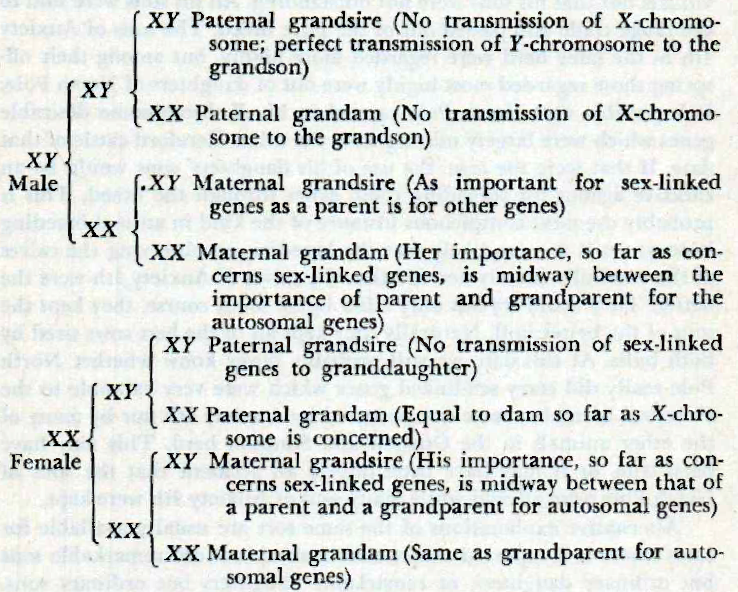
\includegraphics[width=\textwidth]{Page_353.png}
    \label{fig:Lush_Page_353}
    \index{Inbreeding|)}
    \index{Mating like to like}
    \index{Mating unlikes}
    \index{Outbreeding|)}
    \index{Random mating|)}
    \index{Selection|)}
\end{figure}

The above classification may make clearer the kinds and definitions of breeding systems.
\index{Breeding systems for varied purposes|)}

%\textsc{Breeding Plans Based on Selection}
\chapter[How Selection Changes a Population]{How Selection Changes the Genetic Composition of a Population}
\label{cha:how-selection-changes-genetic-composition-population}
\index{Gene frequency|(}
\index{Selection|(}

Causing or permitting some kinds of individuals to produce more
offspring than other kinds do is selection. It is the number raised and
added to the breeding herd rather than the number born which matters,
since those which are born but get no chance to reproduce cannot
affect the composition of the future population. Under some circumstances
selection may quickly cause large and permanent changes in the
population. Under other circumstances it may cause marked changes,
but the moment selection is relaxed the population returns to its original
condition. Under still other circumstances selection may be almost
powerless to produce any change unless it is combined with some mating
system like inbreeding.

The changes which selection produces in the underlying genetic
composition of a population can rarely if ever be seen or measured
directly, since the observer will not know what genes are present, nor
the frequencies of each, nor the frequencies of their various combinations,
nor the amount of change which selection makes in those.

\index{Additive effects of genes}Selection creates no new genes. It merely
causes the possessors of
some genes or of some combinations of genes to have more offspring
than those which lack those genes or combinations. Its primary genetic
effect is to change gene frequency and the frequency of gametes carrying
certain gene combinations. All its other effects are consequences of
that, and their magnitude depends on how much the gene and gamete
frequencies were changed. Changes in gene frequency are permanent
even if selection ceases, unless counter-selection in the opposite direction
begins and is effective. Changes in gamete frequency, other than
those which result from changes in gene frequency, are temporary
because the genes recombine when segregation takes place in forming
the gametes for the next generation. Because of this segregation and
recombination, the gains from selecting for \index{Epistatic effects}epistatic differences are
temporary, and selection must be continued merely to hold those,
although the gains from selecting for additive differences are permanent
and remain even when selection is relaxed and abandoned.

Selection can be creative only in the sense that new types can be
produced when selection has moved the average of the population far
from the original position, as is shown in Figure~\ref{fig:Lush_Figure_15}. For example, suppose
there arc five desirable genes, each having a frequency of .1. If
mating is random, only one individual in ten billion will be homozygous
for all five of the desired genes. For practical purposes this is nonexistent.
But if selection in favor of the individuals with the larger
number of these genes were practiced long enough to raise the frequency
of each gene to .7, then about 28 individuals in each thousand would
be homozygous for all five genes. This is frequent enough that some of
them would be found. In that sense selection may be said to have created
something new, somewhat as an architect can create a building of
an original design, although all the materials were already in existence
before he began.

\section*{ONE PAIR OF GENES}
\index{Homozygosis}

If from a population containing the three genotypes, \textit{AA}, \textit{Aa}, and
\textit{aa}, only the \textit{AA} individuals are allowed to reproduce, the next
generation will be homozygous for \textit{A} which will then have a frequency of 1.0
in that population. Selection will in one generation have done all it
could if it were to be continued for many generations. Similarly, if only
the \textit{aa} individuals had offspring, the whole population in the next generation
would be homozygous for \textit{a}, the frequency of \textit{A} would have
fallen to zero and change by selection would come to an end, as far as
that pair of genes is concerned. In actual practice, selection can practically
never be that accurate and extreme. Instead, some of the undesired
genotypes are kept and some of the desired ones are culled, either
because there are not enough of the desired ones to permit culling all
the others, because the breeder is careless, or because dominance and
environmental variation mislead him. The net result is that selection
increases the frequency of the favored gene by at least a little each generation
and thus leads to some change in the genetic composition of the
population.

There may not be enough individuals to permit discarding at once
all of the undesired ones. If all Shorthorn breeders were to decide suddenly
that they wished their breed to be white, there are probably not
enough white Shorthorn bulls alive that every breeder could secure a
white bull to head his herd, even if no attention were paid to anything
but color. Some would have to use roan bulls for at least a generation
until the number of white bulls had increased. As for cows, they would
not only have to use all the whites but probably all of the roans and
even some of the reds. In the next generation they might have enough
whites and roans that they could cull all of the reds, but it would
probably be several generations before they could discard all of the roan
cows.

The animal is the smallest unit which the breeder can select or
reject, but in the animal the genes come in pairs rather than singly.
This makes progress by selection slower than if selection could be gene
by gene. For example, suppose 25 per cent of the animals in a Shorthorn
population were white, 50 per cent were roan, and 25 per cent
were red, and the breeders should suddenly decide that they wanted the
breed red, but could only afford to cull half of each generation. The
best they could do in the first generation would be to keep all of the
red animals and half of the roans, discarding the whites and the other
half of the roans. There were enough genes for red in the population
that the breeders could have discarded all the genes for white and have
changed the population completely in one generation if they could
have selected gene by gene, but instead they must select or reject the
genes a pair at a time. Selection between zygotes thus changes gene
frequency more slowly than selection between gametes would. It seems
unlikely that the breeder will ever be able to select between gametes,
although some natural selection at that stage does take place in plants
and perhaps some also in animals.

The effects of environment may duplicate or hide the effects of
genes, thus causing the breeder to discard some animals which he would
keep and to keep others which he would discard if he knew what their
genotypes really were. Dominance may do the same thing by preventing
him from knowing which individuals are \textit{AA} and which are \textit{Aa}.
Naturally every mistake of this kind means that the undesired genes are
transmitted by more individuals and the desired genes by fewer than
would have been the case if these mistakes had been avoided. Such mistakes
lower the rate at which selection increases the frequency of the
desired gene. They do not stop the process but merely cause more time
to be required to produce the same amount of change.

\section*{RATE OF CHANGE IN GENE FREQUENCY}

The amount which gene frequency is changed by one generation of selection
could be computed if we knew the rates of reproduction for each of the
three genotypes and the frequency of each genotype. If the numbers of
offspring produced by the same number of \textit{AA}, \textit{Aa}, and
\textit{aa} individuals are in the ratio: 1 : $1 - hs$ : $1 - s$, we can
consider \textit{s} as a measure of the intensity of selection against the
\textit{aa} individuals and \textit{hs} as measuring the intensity of
selection against the heterozygote. For example, if for every 100 offspring
which \textit{AA} individuals produced, the same number of \textit{Aa}
individuals would on the average produce 95 offspring and an equal number of
\textit{aa} individuals would produce only 80 offspring, then \textit{s}
would be .2, \textit{hs} would be .05, and hence \textit{h} would be .25.
In a random breeding population the change ($\Delta q$) produced in the
frequency (\textit{q}) of gene \textit{A} by one generation of selection is
a tiny bit larger than $sq(1 - q)[1 - q + h(2q - 1)]$. The height of the
three curved lines in Figure~\ref{fig:Lush_Figure_13} shows how large
$\Delta q$ would be at each value of \textit{q} and for each of three
conditions of \index{Dominance|(}dominance. The values of \textit{h} are, respectively 0, .5,
and 1. \index{Heterozygosis|(}Selection is most effective, ($\Delta q$ is largest) when gene
frequency is somewhere near the middle of its possible range, and is least
when \textit{q} is near zero or 1.0.

\begin{figure}
	\centering
    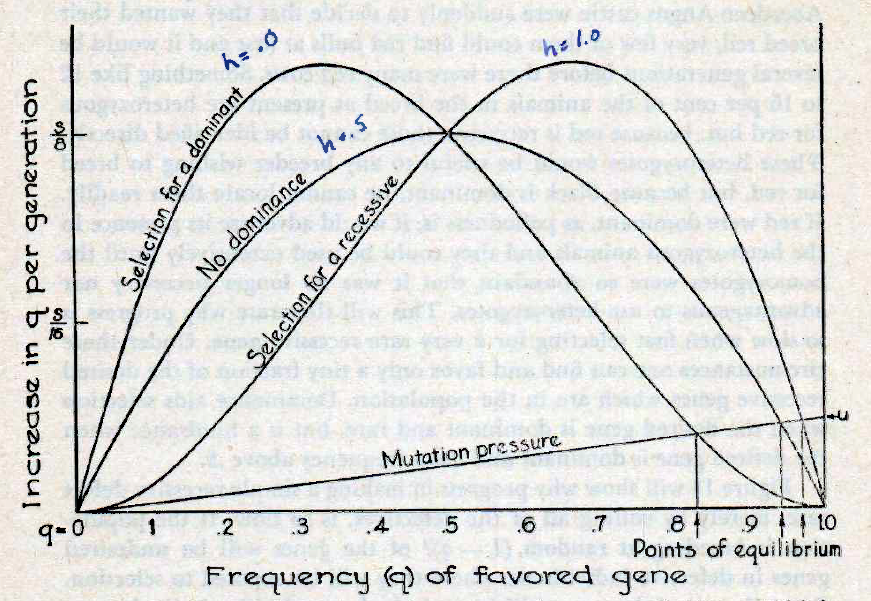
\includegraphics[width=\textwidth]{Figure_13.png}
    \caption{Rate of change in gene frequency under constant selection, \textit{s},
    		 which is opposed by a constant mutation rate, \textit{u}. Drawn with
    		 \textit{u} equal to .03 \textit{s}, which is rather weak selection.
    		 The height of the curved lines indicates the rates at which selection
			 would change the frequency, \textit{q}, of the desired gene under the
			 three conditions specified for dominance. The height of the straight line,
			 ``mutation pressure,'' indicates the rate at which mutation would change
			 gene frequency in the absence of selection. The difference between the
			 height of the curved lines and the height of the ``mutation pressure''
			 line indicates the net rate at which gene frequency is changed by selection
			 and opposing mutation. Arrows indicate gene frequencies at which selection
			 pressure and opposing mutation pressure are equal. (After Wright in
			 \textit{Genetics}, 16:104.)}
    \label{fig:Lush_Figure_13}
    \index{Selection!against recessives}
\end{figure}

\index{Homozygosis|(}
Dominance of the favored gene is a help to selection when that gene
is rare, but a hindrance when the favored gene is more abundant than
the undesired recessive. Thus, those who are breeding Hereford cattle
for polledness are now fortunate that the gene they want is dominant,
because that enables them to distinguish between the heterozygotes and
the homozygous recessives. The gene for polled is still rare enough in
the Hereford breed that its frequency can be increased by using heterozygous
animals for breeding purposes and there are not yet enough
homozygous polled animals to permit discarding all of the heterozygotes.
If the trend toward polledness continues long enough, the time
will come when the favored gene will be more abundant than its recessive
allel. Then the breeders will want to discriminate more strongly
against the heterozygous polled animals. When that time comes, they
will wish that the gene for polledness were recessive. If breeders of
Aberdeen-Angus cattle were suddenly to decide that they wanted their
breed red, very few of them could find -red bulls at first and it would be
several generations before there were many red cows. Something like 12
to 16 per cent of the animals in the breed at present are heterozygous
for red but, because red is recessive, those cannot be identified directly.
These heterozygotes would be useful to any breeder wishing to breed
for red, but because black is dominant, he cannot locate them readily.
If red were dominant, as polledness is, it would advertise its presence in
the heterozygous animals and they could be used extensively until the
homozygotes were so abundant that it was no longer necessary nor
advantageous to use heterozygotes. This will illustrate why progress is
so slow when first selecting for a very rare recessive gene. Under those
circumstances one can find and favor only a tiny fraction of the desired
recessive genes which are in the population. Dominance aids selection
when the desired gene is dominant and rare, but is a hindrance when
the desired gene is dominant and has a frequency above .5.

Figure~\ref{fig:Lush_Figure_13} will show why progress in making a simple
recessive defect rare, merely by culling all of the defectives, is so slow.
If the population is breeding at random, $(1 - q)^2$ of the genes will be
undesired genes in defective individuals, where they will be exposed to
selection. But $q(1 - q)$ of the genes will be undesired genes hidden in the
heterozygous individuals. Thus \textit{q} of the undesired genes will be in
heterozygous individuals where dominance shields them against selection. This
becomes a larger and larger fraction as the undesired recessive becomes rarer.
Consequently, although discarding the defectives is always to be recommended
if the defect is serious, and will decrease the proportion of defectives
rapidly when they are abundant, it produces only slight changes when the
defectives are already rare. Selection is abundantly able to make an undesired
gene rare but is almost powerless to elminate it entirely from the
population.\footnote{Among the nonrandom mating systems, only inbreeding alters
this situation much. Under it the heterozygotes shield from selection only
$q(1 - F)$ of the undesired genes, \textit{F} being the inbreeding coefficient
(Chap. 21) and ranging from $0$ to $+1.0$.}

It is sometimes said that selection makes more rapid progress at first
and that further progress per generation becomes slower and slower.
Inspection of Figure~\ref{fig:Lush_Figure_13} will show that this need not be so. If the desired
gene is very rare, the increase in gene frequency made by selection
would be small at first, simply because there is not enough genetic variability
in the population. As the gene frequency rises toward the values
near the middle of its range, progress would become faster and faster
until it reached a maximum. After that it would decrease.

In actual practice \textit{s} cannot be large against many genes unless each
is rare, as lethals\index{Lethal genes|(} are. If 10 per cent of the population is \textit{aa},
10 per cent is \textit{bb}, 10 per cent is \textit{cc}, etc. each of these
being undesirable; and if many
such traits are to be considered, it will be impossible to find animals
which are free from all of these defects. In any population which is
constant in numbers, at least enough offspring must reach breeding age
to replace their parents. Some animals which have a few defects must
be saved for breeding because they are better than average in other
respects. Any mistakes caused by dominance or by the confusing effects
of environment will also decrease \textit{s}. Since many genes affect the net
desirability of each animal it is reasonable to use a general value something
like .01 for \textit{s} in these formulas, although of course \textit{s} will vary
widely from one gene to another. It will be as high as 1.0 for lethals and
doubtless will approach zero for many genes. In actual practice \textit{s} is likely
to change as selection changes the population. Then more intense
selection for some genes may become possible, and less intense selection
than formerly may be needed for others.

We can compute how many generations will be required to change
gene frequency from one value to another if \textit{s} is known and remains
constant and if the frequencies of the different genotypes are known.
The figures necessary for such computations\footnote{They are derived
from integrating the equations for $\delta q$ under those three
special conditions of dominance. The correction factors in the last column and
in the bottom row allow for a denominator which is not quite 1.0.} are shown in Table 10 for
a random mating population. These figures will show how much time
selection may need for increasing the frequency of a gene by a large
amount. Other than for demonstrating this principle Table 10 is not of
much practical use since one will rarely know the frequency of any of
the genes in his herd. Still more rarely will he know how intense his
selection for each gene actually is. The following example will show
how Table~\ref{tbl:Lush_Table_10} may be used. The time required to change
\textit{q} from .01 to
.05 when selecting for a complete dominant is $\frac{1.69}{s}$
generations, which  equals 169 generations if $s = .01$, but only 1.69
if $s= 1.0$. In either case there is a correction, 1.61, to be subtracted.
The final answer is a little more than 167 generations for the mild selection,
and only .08 generations for the intense selection. For the same problem,
except that selection is for a complete recessive, the final answers are
8,083 generations for the mild selection and .04 generations for the intense
selection. The corrections in the right-hand column, to be used as indicated at the bottom
of the table, are unimportant when \textit{s} is small but are considerable
when \textit{s} is large.

\begin{table}[htbp]
	\centering
	\caption{\textsc{Approximate Time Required for Selection to Increase the Frequency}
			 ($q$) \textsc{of a Favored Gene by Various Amounts}}
	\label{tbl:Lush_Table_10}
	\begin{tabular}{C{1.5cm}|C{1.5cm}|C{1.5cm}|C{1.5cm}|C{1.5cm}|C{1.5cm}}
		\hline
		\hline
		\multicolumn{2}{C{3cm}|}{$q$ to be Changed From $q_1$ to $q_2$} & \multicolumn{3}{C{4.5cm}|}{Time, Expressed in $1/s$ Generations} & \\
		\cline{1-5}
		$q_1$ & $q_2$ &  Selection for a Complete Dominant ($h = 0$) & Selection When There Is No Dominance ($h = .5$) & Selection for a complete Recessive ($h = 1.0$) & Correction Factor \textit{x} \\
		\cline{1-2}
		\hline
		.01	& .05	& 1.69		& 3.30	& 81.65	& 1.61 \\
		.05 & .10	& .81		& 1.49 	& 10.75	& .69 \\
		.10 & .20	& .95		& 1.62	& 5.81 	& .69 \\
		.20 & .30 	& .72 		& 1.08 	& 2.21 	& .41 \\
		.30 & .40	& .68		& .88 	& 1.28 	& .29 \\
		.40 & .50 	& .74 		& .81 	& .91 	& .22 \\
		.50 & .60 	& .91 		& .81 	& .74 	& .18 \\
		.60 & .70 	& 1.28 		& .88 	& .68 	& .15 \\
		.70 & .80 	& 2.21 		& 1.08 	& .72 	& .13 \\
		.80 & .90 	& 5.81 		& 1.62 	& .95 	& .12 \\
		.90 & .95 	& 10.75 	& 1.49 	& .81 	& .05 \\
		.95 & .98 	& 30.95 	& 1.89 	& .98 	& .03 \\
		.98	& .99	& 50.70		& 1.41	& .71	& .01 \\
		.99	& .995	& 100.70	& 1.40	& .70	& .00 \\
		\hline
		\multicolumn{2}{C{3cm}|}{From answer \textit{in generations} subtract:} & $x$ & $2x$ & $x + 1/q_1 - 1/q_2$ & \\
		\hline
	\end{tabular}
\end{table}
\index{Heterozygosis|)}
\index{Homozygosis|)}

\section*{EQUILIBRIUM BETWEEN SELECTION AND OPPOSING MUTATION}
\index{Equilibrium between selection and mutation|(}
\index{Mutations|(}

Mutations are very rare, and nearly all of them are harmful. Therefore
they are to be considered as opposing selection, although perhaps
at extremely rare intervals a favorable mutation does occur. The more
abundant the desired genes are, the more of them are exposed to the
risk of mutating to something less desirable. Hence the higher the frequency
of the desired gene, the more strongly mutation tends to lower
that frequency. That is shown in Figure~\ref{fig:Lush_Figure_13} by the height of the straight
line which shows ``mutation pressure.''

Selection will be a far more powerful force than mutation except
when the undesired gene is very rare. This gives rise to an equilibrium
value for gene frequency at a point where the undesired gene is already
so rare that the few undesired genes eliminated each generation by
selection are balanced by an equal number newly produced by mutation.
A numerical example may make this clearer. If there is perfect
selection against recessive gene \textit{a} ($s = 1.0$) in a random breeding population
of a million individuals, and if the mutation rate from \textit{A} to \textit{a} is
such that in each generation one out of every million \textit{A} genes mutates
to \textit{a}, then the equilibrium point for $q_A$ will be about .999. At that point
the proportion of \textit{aa} individuals born will be 1 in 1,000,000, while
about 1 in 500 will be \textit{Aa}. Culling the \textit{aa} individuals will in each generation
eliminate two \textit{a} genes from every 2,000,000 genes in that allelic
series in that population: At the same time there will be 1,998,000 \textit{A}
genes exposed to mutation. A mutation rate from \textit{A} to \textit{a} of about 1 in
1,000,000 will provide two new \textit{a} genes each generation to replace the
two culled by selection, and the frequency of \textit{A} will not change, even
though selection for it continues.

A general formula for the value of \textit{q} at the equilibrium point may
be had by letting \textit{s} equal the selection coefficient as before and \textit{u} equal
the net rate of opposing mutation. Then an undesired complete recessive
is at equilibrium when its frequency is approximately $\sqrt{u/s}$. The
corresponding equilibrium point for an undesired dominant is $u/s$
and for an undesired gene where the heterozygote is exactly intermediate
in undesirability is $2u/s$. All these frequencies at equilibrium will
be low if \textit{s} is large. Complete dominance shields the undesirable recessive
from selection to such an extent that at equilibrium its frequency is
$\sqrt{s/u}$ times as large as that of an equally undesired dominant. Since \textit{s}
to be detectable would usually need to be larger than .01, and \textit{u} seems
usually to be something of the order of .000,01 to .000,000,1, it is not at
all surprising that undesired recessive genes should be anywhere from
thirty to a thousand times as frequent as undesired dominant genes in a
population which has long been under selection. This may be the major
explanation for the widely observed fact that recessive genes, uncovered
by inbreeding or otherwise, are nearly always less desirable than their
dominant alleles.

\begin{wrapfigure}{L}{0.2\linewidth}
	\centering
    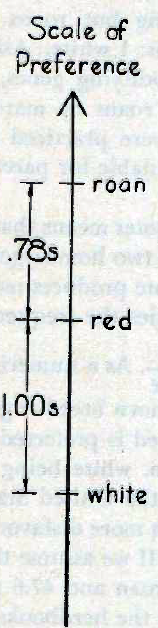
\includegraphics[width=\linewidth]{Figure_14.png}
    \caption{Scale showing the average degree of preference for roan over red and
    		 for red over white among Shorthorn breeders if this preference for the
    		 heterozygote is the only thing holding these colors in constant proportions in the breed.}
    \label{fig:Lush_Figure_14}
\end{wrapfigure}

\section*{ABUNDANCE OF RECESSIVE UNDESIRABLE GENES}

While $\sqrt{u/s}$ is a very low equilibrium frequency for any one gene
which is seriously undesirable, yet if the number of loci which can
mutate to undesired alleles is several hundreds or a few thousands, as
the evidence indicates, then the total number of lethal genes which can
exist in the population is large. It might happen that nearly every individual
would carry at least one lethal, although only rarely would the
male and female which mate together both carry the same lethal gene.
If so, the proportion of defective individuals born would be small, as
long as the population is large and mating practically at random, but
would increase sharply whenever inbreeding is begun. As a numerical
example, suppose \textit{u} is .000,001, \textit{s} is 1.0 as it would be for a lethal gene,
and \textit{h} is zero as it would be for a completely recessive lethal which had
no desirable effects at all. Then the frequency of a lethal gene would be
maintained at about .001 in a very large and freely interbreeding population.
Only about one in a million among those born would be homozygous
and die. Yet about one individual in every 500 would carry the
gene and would be capable of transmitting it. If there are 1,000 such
loci capable of supporting lethals at equilibrium frequencies of .001,
only about 14 per cent($=.999^{2000}$) of all individuals will be entirely
free from all lethals. The rest will carry one or more which they could
transmit. Only about one individual in a thousand among those actually
born will show any one of these 1,000 individually rare defects.

These figures will illustrate why lethal or otherwise undesirable
genes may be so abundant in a population that inbreeding will be
almost sure to uncover them in large numbers and yet, if the population
is large and breeding at random, any one of those defects may be
seen only rarely. They will also explain why genes against which selection
has always been directed since time began still recur in appreciable
numbers. Lethals are examples of such genes, although there is always
the possibility that a gene now lethal in combination with the present
genes of the species once may have been neutral or even advantageous
at an earlier stage when the species had other genes.

The actual evidence on the abundance of lethals in farm animals is
still scanty. It consists mostly of the considerable number of lethals for
which the Mendelian basis has been discovered and reported already
and of general observations concerning the effects of inbreeding. There
is more evidence concerning natural populations of such organisms as
Drosophila, although the question of whether the situation is the same
among farm animals remains an open one. For example in one study
(\textit{Genetics} 26:25) of \textit{Drosphila pseudoobscura} from the Death Valley
region in California, over 15 per cent of all third chromosomes in wild
flies carried lethals. In another population from Mexico and Guatemala
the corresponding figure was 30 per cent. In another California population
(\textit{Genetics} 27:373) of 1,292 chromosomes the figure was 14 per cent.
Another study (\textit{Biological Symposia} VI:18) of New England, Ohio, and
Florida wild populations of \textit{Drosophila melanogaster} showed that 41 to
67 per cent of the second chromosomes carried lethals or semilethals.
While such evidence is still meager, yet it seems to indicate that few
individuals are absolutely free from all undesired genes. A small
amount of the breeder's freedom to select will be used in combating
the generally destructive tendencies of mutation.
\index{Equilibrium between selection and mutation|)}
\index{Mutations|)}

\section*{SELECTION IN FAVOR OF THE HETEROZYGOTE}
\index{Equilibrium between selection and mutation!when selecting for a heterozygote|(}
\index{Heterosis|(}
\index{Heterozygosis|(}
\index{Heterozygote preferred|(}
\index{Selection!against recessives}
\index{Selection!for heterozygotes|(}

Selection can never fix the heterozygote. Examples of such heterozygotes
are the Blue Andalusian fowl, the Erminette fowl, the cream color
of guinea pigs, the yellow color of mice and the roan color of such
breeds of cattle as the Shorthorn, the Blue Albion, the ``race bleue'' (in
France), and the blue color inside the ears of Wensleydale sheep, and
the Palomino color in horses. Selection of nothing but roans in
Shorthorns would lead toward a ratio of 1 red: 2 roans: 1 white. Aside
from a few exceptions possibly caused by other modifying genes, it
would be possible to produce calves which all were roans by mating
whites to reds, but that would be temporary if it were practiced all
over the breed, because only roans would then be available for parents
of the next generation.

Preference for the heterozygote over both homozygotes means that \textit{h}
in the general formula for $\Delta q$ is negative. One of the two homozygotes
may be preferred over the other, but if the heterozygote produces more
offspring than either homozygote, such selection carries the frequency
of the gene toward a stable equilibrium value, $\dfrac{1-h}{1-2h}$. As a
numerical example we may take roan color, which in the Shorthorn breed is generally
preferred over both white and red, although red is preferred to
white. These preferences vary from region to region, white being in
more disfavor in the southern and western parts of the United States
than it is in the eastern Corn belt or in Canada, and in more disfavor in
the Argentine and South Africa than it is in Britain. If we assume that
Wright's count of 8.6 per cent white, 43.8 per cent roan and 47.6 per
cent red among 6,000 animals, equally distributed in the herdbooks of
the United States, Canada and Great Britain, represents the equilibrium
condition of the breed with respect to color, and if we further accept
the monofactorial explanation of the inheritance of these colors, then,
by setting $\Delta q$ equal to zero a numerical expression can be had for the
degree to which roan is preferred over red and to which red is preferred
over white. That is shown graphically in Figure~\ref{fig:Lush_Figure_14}. The
example illustrates how a population can cease to change while yet selection for a
heterozygote continues and \textit{q} has an intermediate value. The example
is particularly instructive in showing how it can happen that the most
highly preferred color (the roan) is not necessarily the most abundant
when equilibrium is reached. This happens because red is preferred to
white even more than roan is preferred to red.
\index{Dominance|)}

Whether the heterozygote is often preferred over both the homozygotes is not
yet clear. The cases for which the definite Mendelian basis is known are few
but the phenomenon of heterosis, which is widespread and important, is believed
by some to rest almost wholly on this. This is likely to be true if (1) each
gene has several effects\index{Multiple effects of genes} and if (2) the more favorable effect tends to be dominant
over the less favorable effect, regardless of the other effects of the same gene.
If this is generally true, ideal breeding systems for producing maximum vigor,
health, and growth rates, as in animals destined directly for the market, should
 be based even more than at present on maintaining purebred but unrelated seedstocks
 and crossing these for the production of market and work stock.

A preference for the heterozygote may be partly responsible for some lethal genes
being as abundant as they are. The yellow mouse, the ``creeper'' fowl, extreme short
leggedness in Dexter cattle, and probably the abnormally thick muscles of ``doppellender''
cattle, are examples of genes which are lethal when homozygous but have highly prized
dominant effects when heterzygous. If a lethal gene has even one dominant effect,
favorable enough to give the heterozygote a 1 per cent advantage over the more desirable
homozygote, then its equilibrium frequency will be more nearly .01 than .001; nearly 2 per
cent of all individuals would carry it, and one such lethal individual would appear among
each 10,000 born. If the advantage of the heterozygote over the normal is 5 per cent, the
lethal gene will have an equilibrium frequency of $l/21$, nearly 9 per cent of all individuals
would carry it, and about one individual in 484 would be lethal.
\index{Heterozygosis|)}
\index{Lethal genes|)}

\section*{INTENSITY AND DIRECTION OF SELECTION MAY VARY WITH GENE FREQUENCY}

The conditions under which and the purposes for which the breed is kept may be complex
enough that there is need for at least a few of each genotype, just as in human societies
there is an economic need and reward (an \textit{ecological niche}, the biologist would
say) for a few each of tailors, bakers, lawyers, doctors, etc., but if any
one of these professions becomes overcrowded, its members are at a
competitive disadvantage. If there is no pedigree barrier to the free
interbreeding of types in similarly complex animal populations, the
result is the same as if the heterozygote were preferred; namely, gene
frequency is rather quickly carried to near the value which will furnish
the optimum ratio between each of the two homozygotes and the heterozygotes
under those conditions. In terms of the general formula this
means that the size and even the sign of sand of \textit{h} depend in part on
\textit{q}. Little is known definitely about whether this situation is rare or
widespread and important, either in animal breeding or in nature. Presumably
it will be frequent wherever ecological or economic conditions are highly varied.
\index{Equilibrium between selection and mutation!when selecting for a heterozygote|)}
\index{Heterosis|)}
\index{Heterozygote preferred|)}
\index{Selection!for heterozygotes|)}

\section*{SELECTION AND HOMOZYGOSIS}
\label{sel_and_homozyg}
\index{Selection!and homozygosis|(}

Selection changes homozygosis but little in any one generation. Such
change as it does produce may be either to increase or to decrease homozygosis.
If mating is random among those selected to be parents,
$2q(1 - q)$ of the whole generation out of which the parents are selected
will be heterozygous and $2(q + \Delta q)(1 - q - \delta q)$ of the next generation
will be heterozygous. The change in heterozygosis will be
$2 \Delta q (1 - 2q - \Delta q)$ which will depend on both $\Delta q$ and \textit{q} for its size
and will be negative when \textit{q} is larger than .5, provided that selection
does have some effect and hence that $\Delta q$ is positive. As numerical examples,
consider first a case where $q = .2$ and selection is so effective that
$\Delta q = .03$, and then a case where $q = .7$ and selection again is effective
enough that $\Delta q = .03$. In the first case heterozygosis was .32 in the parental
generation and rose to .3542 in their offspring. Here the successful
selection decreased homozygosis by .0342. In the second case heterozygosis
was .42 in the parental generation and fell to .3942 in the offspring.
Here the successful selection increased homozygosis by .0258.

Referring back to Figure~\ref{fig:Lush_Figure_3} it will be noted that
$2q (1 - q)$ changes only a little with changes in \textit{q} while \textit{q}
has values near the middle of its range. It does change rather rapidly with
changes in \textit{q} when \textit{q} is near zero or 1.0, but those are the values
of \textit{q} at which selection cannot change \textit{q} rapidly. Hence, under any
but laboratory conditions, where selection might perhaps be extremely intense and
directed entirely at the effects of one gene, selection has only tiny effects in any
one generation on the homozygosity of the population. This is in marked contrast to
the rather powerful effects it can have on the mean of the population when \textit{q}
is near .5.

Among the nonrandom mating systems, only inbreeding will
increase homozygosity much. The amount of help or hindrance which
selection will be to inbreeding in that respect will be so small in any one
generation that for practical purposes it can be disregarded, although
the accumulated effects may become important if selection is continued
over many generations and if the inbreeding is mild.
\index{Selection!and homozygosis|)}

\section*{SELECTION AND SEX-LINKAGE}
\index{Selection!and linkage}
\index{Sex linkage}

Selection between sex-linked genes is more effective in the heterogametic
sex than in the homogametic sex, both because the deceiving
effects of dominance are absent and because the heterogametic sex
shows the gametic ratio of sex-linked genes directly instead of the
square of that ratio as the homogametic sex does. If \textit{s} against \textit{a}-- individuals
is the same as \textit{s} against \textit{aa} individuals, $\Delta q$ pertaining to sex-linked
genes in the heterogametic sex is exactly twice as large as it is for
an autosomal gene which shows no dominance at all. In the homogametic
sex, selection for sex-linked genes proceeds at exactly the same
rate as selection for equally desirable autosomal genes.

\section*{MANY PAIRS OF GENES-SIMPLEST CONDITIONS}
\index{Variation!as affected by gene numbers|(}

If there are \textit{n} pairs of genes equal in effects, without dominance or
epistasis, and if the characteristic is not affected by the variations in
environment within that population, then the range between the most
extreme individuals possible is \textit{2n} and the standard deviation is
$\sqrt{2nq(1-q)}$ times the effect of one gene. Thus the range is
$\sqrt{\frac{2n}{q(1-q)}}$ times the standard deviation. Individuals varying from the
mean of a normal population by as much as two times the standard
deviation in either direction are unusual (l in 22), while those varying
as much as three times are quite rare (l in 370), and those varying more
than four times scarcely occur at all except among truly enormous
populations. Consequently, if the ideal is an extreme type and if more
than three or four pairs of genes are involved, individuals homozygous
for the desired genes may be so rare that they do not exist at all in the
population from which the initial selections must be made. Perfect animals
cannot be selected for parents simply because they have not yet
been born! Instead the best of those available will be selected and, as
this increases the frequency of the genes with the desired effects, each
generation will average nearer to the desired goal than the preceding
one did, but several generations of selection may be necessary before
any ideal individuals appear. The rate of improvement from one generation
to the next rises or falls with the standard deviation and therefore
is generally maximum when gene frequencies are near .5. Improvement
continues until the goal is eventually reached, or selection comes
into equilibrium with opposing mutation rates. The distribution of
the population becomes increasingly asymmetrical as the goal is
approached. This is the situation usually pictured in generalized discussions
of the results of selection. It is represented in Figure~\ref{fig:Lush_Figure_15},
where selection begins when the frequencies of all gene pairs are .5, as, for
example, in an $F_2$ generation. Environmental effects and dominance
change this situation chiefly in making progress per generation slower,
and the changes in variability and symmetry less.

\begin{figure}
	\centering
    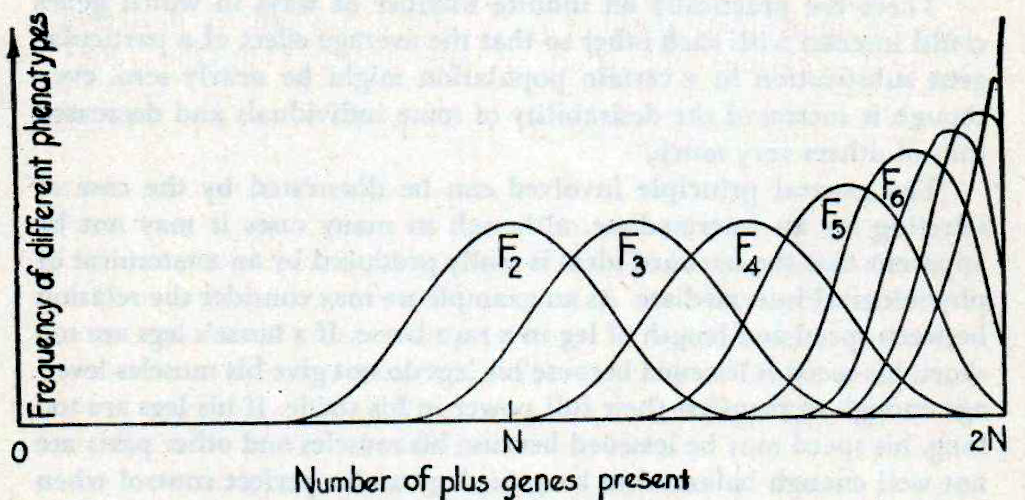
\includegraphics[width=\textwidth]{Figure_15.png}
    \caption{Distribution of successive generations under intense selection toward an
			 extreme, with few mistakes from dominance or from environmental causes and with
			 no epistasis.}
    \label{fig:Lush_Figure_15}
\end{figure}

As \textit{n} increases, $\Delta q$ for each gene decreases, other things being equal.
But, since the effects of more genes are involved, the rate of change in
the population mean, which is proportional to $2n{\Delta}q$, is unaffected.
Changes in things like the variability and homozygosity of the population,
which depend on the rate of change in \textit{q}, are made slower as \textit{n}
increases. But for the practical breeder the main difference resulting
from whether a fixed amount of variability is caused by many genes
each with small effects or by a few genes each with large effects is that in
the former case the ultimate limit to which the population mean can
be carried is much farther off, and he can expect progress per generation
to be steadier and not to increase or decrease so much or so soon as
in the latter case.
\index{Variation!as affected by gene numbers|)}

Doubtless some genes have large and some have small effects.
Because of that, the variability of the population behaves as if n were
smaller than the actual number of genes but larger than the number of
those which have major effects. ${\Delta}q$ will be larger for the genes with the
larger effects than for genes with minor effects. When selection succeeds
in making \textit{q} for the more important genes approach such high values
that they no longer contribute much to the genetic variability of the
population, the situation becomes more nearly as if many genes each
have minor effects.

\section*{SELECTION FOR EPISTATIC DIFFERENCES}

Some genes have one effect in some combinations and another effect
in other combinations. In combination with \textit{Aa} or \textit{AA}, \textit{bb} may have an
undesirable effect, and \textit{aa} may have an undesirable effect when in combination
with \textit{BB} or \textit{Bb}; but \textit{a} and \textit{b} may supplement each other's
effects so well that \textit{aabb} is as desirable as \textit{AABB}. In such a case it would
be meaningless to speak of \textit{A} or \textit{B} as desirable genes. They are desirable
when together but undesirable when separate. Selection for net merit is
against \textit{A} when \textit{B} is absent but for \textit{A} when \textit{B} is present. A partial analogy
may be had by considering whether shoes help or hinder the speed
of a man running a foot race. If he takes off one shoe, his speed will
almost certainly be lowered; but, if he takes off the other one also, his
speed will be raised again, perhaps even to a higher level than when he
wore both shoes. Whether taking off a shoe makes him faster or slower
depends in part on whether the other shoe is on or off!

There are practically an infinite number of ways in which genes
could interact with each other so that the average effect of a particular
gene substitution in a certain population might be nearly zero, even
though it increased the desirability of some individuals and decreased
that of others very much.

The general principle involved can be illustrated by the case of
selecting for an intermediate, although in many cases it may not be
apparent that the outward ideal is really produced by an anatomical or
physiological intermediate. As an example we may consider the relation
between speed and length of leg in a race horse. If a horse's legs are too
short, his speed is lessened because his legs do not give his muscles leverage
enough to manifest their full power in his stride. If his legs arc too
long, his speed may be lessened because his muscles and other parts are
not well enough balanced to keep his legs under perfect control when
racing. The maximum of speed may come neither with extremely long
nor extremely short legs but with legs perfectly balanced with other
parts so that the animal is a harmonious whole with all parts co-operating
perfectly with each other. The genes which affect the length of leg
might be entirely additive in their effects on length of leg, but they will
not be additive in their effects on speed.

This simple situation is illustrated in Figure 16. The change from \textit{a}
to \textit{A} may tend to make a horse's legs longer, almost regardless of how
long they already are or of what other genes are present, but it will not
consistently make the horse speedier or slower. We may speak of \textit{A} as a
gene which lengthens legs. We cannot consistently speak of it as a gene
which makes a horse speedier. If substituted for \textit{a} in a short-legged
horse, it makes him speedier; but, if the same gene substitution is made
in a long-legged horse, it makes him slower. Selection for speed is selection
for \textit{A} in short-legged horses and selection against \textit{A} in long-legged
horses.

\index{Equilibrium between selection and mutation!when selecting for an intermediate|(}
\index{Selection!for intermediate|(}
\label{page135}
The simplest scheme which will describe in Mendelian terms the
consequences of selecting for an epistatic effect is to suppose that a characteristic
is affected by two pairs of genes lacking dominance, equal in
effect, and combining their effects by addition, but that the intermediate
phenotype --- the one with two plus genes --- is considered the most
desirable. If in each pair the gene with the plus effect has a frequency of
.5, the nine possible genotypes will be grouped into five phenotypes as
follows:

\begin{table}[htbp]
	\centering
	\begin{tabular}{L{3cm}ccccc}
	 	&		&					& \textit{1aaBB}	&					&	\\
	 	&		& \textit{2aaBb}	& \textit{1AAbb}	& \textit{2AaBB}	&	\\
	Genotypes:	& \textit{1aabb}	& \textit{2Aabb}	& \textit{4AaBb}	& \textit{2AABb}	& \textit{1AABB} \\
	\hline
	No. of plus genes in each animal	& 0					& 1					& 2					& 3					& 4 \\
	Ratio of numbers in each phenotype	& 1					& 4					& 6					& 4					& 1 \\
	\end{tabular}
\end{table}

\noindent
Saving for breeding purposes only individuals from the middle phenotype
would increase the proportion of that phenotype in the next generation
from 37\nicefrac{1}{2} to 50 per cent and would reduce the variability of the
population. The breeder would appear to be making rapid progress.
In the second generation of selection the percentage in the most desirable
phenotype would increase from 50 to 56 per cent, and the variance
which was reduced to 67 per cent of its original value by one generation
of selection would be further reduced to 56 per cent of the original.
Progress in the second generation is less than in the first. In the third
generation of such perfect selection for the intermediate phenotype, the
percentage of individuals in that phenotype would rise only from 56 to
57 per cent, and the additional decrease in variance would be only 2 per
cent of the original amount. Progress would come nearly to an end with
the second or third generation of such selection.

\begin{figure}
	\centering
    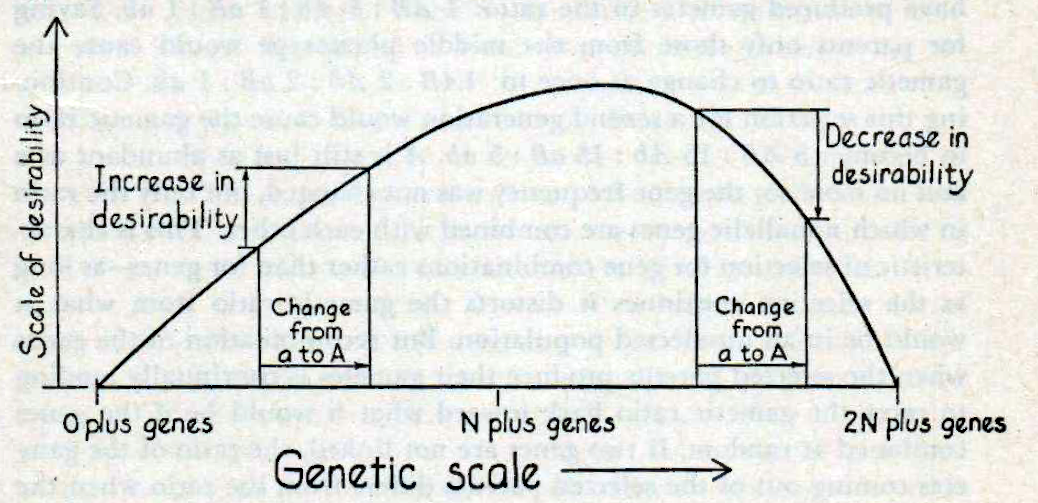
\includegraphics[width=\textwidth]{Figure_16.png}
    \caption{Illustration of a simple case where the most desirable individuals arc
			 intermediates on the genetic scale. Whether the substitution of A for a increases or
			 decreases the merit of the individual depends on the other genes which are present}
    \label{fig:Lush_Figure_16}
\end{figure}

Not only is selection helpless to make much change beyond this
point, but continued selection is necessary to hold the gains already
made. If selection ceased at the end of the third generation, the percentage
of individuals in the desired middle phenotype would fall in
the next generation from 57 to 45 per cent and in another generation or
two would be practically where it was (37\nicefrac{1}{2} per cent) before any selecting
began.

\index{Gametic ratio}\label{page136}
In this example selection was neither for nor against \textit{A} or
\textit{B}; it was for animals which had any combination of two of
those genes. The result was a change in the gametic ratio because
selection eliminated more of the individuals which would produce
extreme gametes (\textit{AB} and \textit{ab}) than of those which
would produce gametes (\textit{Ab} or \textit{aB}) containing only
one of the plus genes. The unselected original population would have
produced gametes in the ratio: 1 \textit{AB} : 1 \textit{Ab} : 1
\textit{aB} : 1 \textit{ab}. Saving for parents only those from the
middle phenotype would cause the gametic ratio to change at once to:
1 \textit{AB} : 2 \textit{Ab} : 2 \textit{aB} : 1 \textit{ab}. Continuing
this selection for a second generation would cause the gametic ratio to
become: 5 \textit{AB} : 13 \textit{Ab} : 13 \textit{aB} : 5 \textit{ab}.
\textit{A} is still just as abundant as \textit{a} and no more so; the
gene frequency was not changed, but only the ratio in which nonallelic genes
are combined with each other. This is characteristic of selection for gene
combinations rather than for genes --- as long as the selection continues it
distorts the gametic ratio from what it would be in an unselected population.
But recombination of the genes when the selected parents produce their gametes
is continually tending to carry the gametic ratio back toward what it would be
if the genes combined at random. If two genes are not linked, the ratio of the
gametes coming out of the selected parents differs from the ratio when the genes
are combined at random only about half as far as did the ratio of the gametes
which united to form those selected parents. With each additional generation,
after selection ceases, the remaining difference between the actual gametic ratio
and what that ratio would be under random combination tends to be halved. If the
two genes are linked the rate of approach toward the random distribution is
\textit{c} (instead of one half) of the remaining difference each generation,
\textit{c} being the percentage of recombination.

Selection for epistatic effects is somewhat like building a sand pile
on the seashore exposed to each incoming wave. It is easy to build a
little pile between waves, but each wave which rolls over it tends to flatten
out the pile. When building is stopped, some traces remain after the
first wave and perhaps even a few after the second and third, but soon
practically all traces of the pile are leveled away. If building continues
between waves, the pile can be built a little higher before the second
and third waves than it was built before the first wave but soon a size is
approached which can just be maintained, the building between waves
being just enough to repair the leveling action of the preceding wave.

It should be emphasized that selection for an intermediate is not
necessarily selection for heretozygosis. In the example just given, selection
was for the \textit{AAbb} genotype which is entirely homozygous, just as
much as it was for the \textit{AaBb} genotype which is entirely heterozygous.
Intermediacy and heterozygosis are almost unrelated to each other, provided
the characteristic is affected by more than two or three pairs of
genes.\label{page_137}

The existence of environmental effects and dominance to confuse in
the selections, and the usual necessity of saving more than one phenotypic
class in order to have parents enough, weaken the intensity of
selection for epistatic gene combinations. Probably the Mendelian
example just used showed more extreme effects than would often be
met in practice, although the multiplicity of kinds of epistatic effects
possible throws some doubt on the validity of that conclusion.

Also this example was somewhat artificial in its supposition that the
frequencies of \textit{A} and of \textit{B} were both exactly .5 and would remain at
that level. If one had been larger and the other smaller, selection would
ultimately have made the whole population homozygous for the gene
with the larger initial frequency and for the allel of the gene with the
smaller initial frequency. The frequencies are in equilibrium when
both are .5, but this equilibrium is essentially unstable. When disturbed
by sampling variations, it would tend to depart from equilibrium at an
increasing rate. Hence, the population would ultimately become either
\textit{AAbb} or \textit{aaBB}. In more complicated epistatic situations the equilibrium
might well be a stable one toward which each gene would tend to
return when disturbed.\label{page137}
\index{Selection!for intermediate|)}

The general principle which the example illustrates is that, where a
genetic intermediate is the goal, selection will carry a population rather
quickly to the point where the number of plus genes will \textit{average} nearly
what is desired, but some individuals will have more of them and some
will have less. Further selections can do little more than hold down the
variation, unless the epistatic equilibrium is an unstable or moving
one. If selection ceases, the average number of plus genes will not
change but variability will at once increase, and the average merit of
the population will decline sharply , most of that decline occurring in
the first generation.

For \textit{all} of the differences caused by the \textit{Aa} pair of genes to be epistatic
requires that the average effect of changing \textit{A} to \textit{a} shall be zero;
i.e., that the cases in which the possessors of \textit{A} have higher reproductive
rates than the possessors of \textit{a} shall be exactly balanced by the cases in
which the possessors of \textit{A} have the lower rates. Then the net selection
pressure for or against \textit{A} (the average \textit{s}) would be zero, and selection
would not tend to change the frequency of \textit{A} in either direction. How ever,
if selection changes the frequency of other genes which alter the
difference between \textit{AA} and \textit{aa}, the proportion of genotypes in which \textit{A}
is at an advantage or disadvantage may change. This would then give \textit{A}
some average effect, and selection for or against it would begin. In
short, \textit{s} for \textit{A} would partly depend on the frequency of genes in other
allelic series, as well as on the physiological differences between \textit{A} and
of \textit{a} themselves and on the kinds and frequencies of the different environments
in which the population lives.

The general effect of epistatic interactions is to decrease the rate at
which selection changes the frequency of a gene, but they may help gene
frequency to drift about irregularly to an extent which may sometimes
be important, especially in small populations being inbred.
\index{Equilibrium between selection and mutation!when selecting for an intermediate|)}

\section*{AUTOSOMAL LINKAGE AND SELECTION}
\index{Linkage|(}
\index{Selection!and linkage|(}

Autosomal linkage makes new combinations rarer. It is therefore a
factor for stability, making it harder to get desired new combinations
but easier to hold existing combinations of desirable genes while trying
to add other genes to them. Although linkage is a drag on progress, it
does not actively tear down any of the breeder's past accomplishments.
It can be compared with friction in a machine which requires effort to
overcome but helps keep the machine in position wherever it stops and
can be useful in such parts of the machine as brakes and governors.

How linkage works can be seen by supposing an extreme case in
which there is no crossing over. Then each chromosome would behave
as one large gene with many effects, some favorable and some unfavorable.
These effects would be distributed more or less randomly along
the chromosome, but it would be a remarkable coincidence if two
chromosomes of a pair were exactly equal in selective value. In the
whole population the chromosomes of each pair would constitute an
indefinitely extended series of multiple alleles. With any general tendency
for dominance of the favorable effects, selection would favor the
heterozygotes and tend toward an equilibrium at which the population
would continue to keep all chromosomes which had any dominant
favorable effects at all. But those chromosomes which had only a few
favorable effects would be kept at a low frequency. As mutations
occurred, the selective values of the chromosomes containing them
would alter, and the equilibrium frequencies would shift.

Now if some crossing over takes place, the selective value of each
chromosome will alter at a still more rapid rate. Any chromosome
which loses more of the desirable genes than it gains by crossing over
tends to be reduced to a lower frequency. One which gains more than it
loses tends to be increased to a higher frequency.

Crossing over is continually tending to bring each pair of genes into
random distribution with every other pair, so that the
\index{Coupling and repulsion}coupling phases
of the double heterozygotes tend to become just as numerous as the
repulsion phases. But whenever the genes are not in this equilibrium,
the approach toward equilibrium is slower if there is linkage than if the
genes were independent. Selection disturbs this randomness of the
combinations of the genes with each other, as will be discussed in more
detail in the section on selection and variability. The gametes coming
from the selected individuals tend to include more of the intermediate
combinations and fewer of the extreme combinations than if the same
genes were combined entirely at random. If linkage exists this will persist
longer and will build up to a wider discrepancy from the random
distribution than if the genes are all independent.

If the population is large enough that the inbreeding\index{Inbreeding} effect can be
ignored, the net result is that linkage will make the offspring of selected
parents less variable, and this in turn will prevent the selected and the
culled individuals in the next generation from averaging as far apart as
they might otherwise. Linkage may constitute some reason for allowing
two or three generations of interbreeding following a cross before selecting
intensely to combine the desirable characteristics of two different
races into one new one. That would give more time for the various
genes to cross over so that their coupling and repulsion phases would
have more chance to become equally abundant.
\index{Selection!and linkage|)}

In selection for such epistatic effects as when the intermediate is
more desirable than either extreme, linkage may play a still more active
part in keeping the percentage of desired offspring higher than it would
be otherwise.\footnote{For details about this see Mather's article in
\textit{Jour. of Genetics} 41: 159--93. 1941.}
\index{Linkage|)}

\section*{SELECTION AND THE VARIABILITY OF A POPULATION}
\index{Selection!and variability|(}
\index{Variation!as affected by selection|(}

Mass selection of the parents has little effect on the variation among
the offspring, although of course the variation remaining among the
selected parents themselves will be distinctly less than was in the population
from which they were chosen.

Eliminating IO per cent of the very poorest from a normal distribution
will decrease the standard deviation of the remainder by 16 per
cent, eliminating 20 per cent will decrease it 24 per cent, and eliminating
50 per cent will decrease it 40 per cent. Thus even a small amount of
culling can make rather striking effects on the uniformity of the group
of survivors. Probably this is the main cause of the rather widely held
opinion that selection is an effective way of increasing uniformity. In
most herds some selection is practiced, and the visitors see only the
selected survivors of at least a little culling. When they do see a herd
where, through the owner's carelessness or financial difficulties or other
reasons, no selection is being practiced they see for the first time that
rather rare sight --- an entirely unselected population. They are likely to
compare such a herd with the other herds they know, which are selected
populations, rather than with the unselected offspring of selected parents.
The latter is what should be done to find how selection of the
parents really affects the uniformity of their offspring.

Sometimes in thinking about selection and variability we are contrasting
two herds which are the products of selection in different directions.
Since selection can shift the mean of a population considerably,
even when it does not change the variability within that population,
two herds started from the same foundation stock but selected toward
different goals for two or three generations may differ rather sharply in
their means. If so, it may appear by contrast that selection has made
each herd uniform, whereas really it only increased the differences
between herds without making much change in the variation within
herds.

Sometimes when we think of selection and uniformity we are comparing
the offspring of one selected sire with a whole breed or other
large population. The offspring of one sire have some extra uniformity
because they are half brothers and hence get half of their inheritance as
samples from the very same genotype. By contrast individuals whose
parents were not the same but merely were selected because they were
much alike phenotypically may get widely different kinds of inheritance,
since those parents will generally be less alike in breeding value
than they are phenotypically.

Often when we think of selection and variability we are comparing
the variation within one herd with variation within the whole breed
Usually each herd has some environmental conditions which are different
from those of other herds but tend to affect alike all the members of
the same herd. These effects of common environment may often be
enough to make each herd distinctly less variable phenotypically than a
population composed of a fair sample from all herds of the breed.

All these things may be mistaken for the effects of selection. One
or more of them often are. It is not surprising that many persons, without
having seen experiments or herds where the actual contrast is only
that the parents were a selected group in the one case and a random
sample of their population in the other, should have inferred that selection
would increase uniformity distinctly. This opinion is still widespread,
notwithstanding the fact that actual experiments have
contradicted it and that these have been published. As long ago as 1907
E. D. Davenport wrote\footnote{Pages 534 and 537 in \textit{Prin. of Breeding.}
Ginn \& Company.} ``We often speak of `fixing' the type by selection,
meaning by that the reduction of variability. All recent studies,
however, go to show that we do not greatly reduce variability by selection,
however much we alter the type.'' and ``The principal function of
selection, therefore, is to \textit{alter the type, not to reduce variability},
$\cdots$''

Selection of the parents alters the variability of the next generation
in two ways from what it would have been if the parents had been
unselected. First, it changes gene frequency, and that automatically has
some effect on variation. Second, the gametes from selected parents
contain a somewhat larger proportion with intermediate combinations
of desirable and undesirable genes than would be the case if the very
same genes with the same actual frequencies were combined entirely at
random.

The first effect is almost always very slight and may either increase
or decrease variability. It has already been discussed in connection with
selection and homozygosis (page \pageref{sel_and_homozyg}). Variance goes up and down in
proportion to a term which always has $2q(1 - q)$ as a factor, the other
factors depending on whether there is dominance and upon the nature
of the mating system, if that is not random. Successful selection will
increase variability if \textit{q} is small at the start but will decrease variability
after \textit{q} is much larger than .5. But the change is very small when \textit{q} has
values in its middle range, and ${\delta}q$ will be small when \textit{q} is near zero or
1.0. Therefore, this effect of selection in changing variability may be
plus instead of minus but is exceedingly small in any one generation.

The other effect of selection in producing an excess of intermediate
gametes, as compared with what there would be if the same genes were
combined with each other entirely at random, is the same process
already discussed (pages \pageref{page136} and \pageref{page137}) in connection with selection for a
genetic intermediate except that here it is usually less extreme, since
individuals are discarded from only one end of the curve and not from
both. As an extreme Mendelian example, consider again the case on
page \pageref{page137} and suppose that only the two phenotypes on the extreme
right were saved for breeding. \index{Gametic ratio}The frequency of \textit{A} and of \textit{B} among the
gametes they produce would both be .8. The actual array of gametes
from those parents as contrasted with what would occur if the same
genes were combined strictly at random would be as follows:

\begin{table}[htbp]
	\centering
	\begin{tabular}{L{4.5cm}C{1.5cm}C{1.5cm}C{1.5cm}C{1.5cm}}
	Gametes				& \textit{ab}	& \textit{Ab}	& \textit{aB}	& \textit{AB}	\\
	Actual frequency	& .00			& .20			& .20			& .60			\\
	Frequency if random	& .04			& .16			& .16			& .64			\\
	\end{tabular}
\end{table}
\index{Selection!for intermediate}

\noindent
Although the example is extreme and selection is assumed to be without
mistake, the departures from the random distribution are small.

This excess of intermediate gametes tends to correct itself in subsequent
segregations and recombinations of the genes. Whatever difference
there is between the actual gametic array and what it would be if
the genes were combined at random tends to be halved with each succeeding
generation, so far as concerns any two unlinked genes, and to
lose \textit{c} of its amount in each generation if the genes are linked,
\textit{c} being the percentage of recombination.

This effect of selection through narrowing the gametic array is generally
slight. It depends for its size on the intensity of selection as well
as on the square of the \index{Heritability}heritability of the characteristic being selected.
As a numerical example, if only the best half of a hitherto unselected
and random breeding population is saved for breeding, the standard
deviation of the offspring will be 17 per cent less than the standard
deviation of the population from which their parents were taken if the
characteristic being selected is not affected at all by environment, dominance,
or epistasis. But if heritability is 50 per cent, the reduction in
standard deviation will be only 4 per cent. If heritability is as low as 30
per cent the reduction in standard deviation will be less than 2 per
cent. If the culling could be so extraordinarily intense that only the
best 10 per cent were saved for parents, the corresponding reductions in
standard deviations for those three levels of heritability would be 24
per cent, 5 per cent, and 2 per cent, respectively. For characteristics with
heritabilities much under 50 per cent, the reduction in the variability
of the offspring caused by selection of the parents is thus only a tiny
amount.

The reduction in variability proceeds only a little farther in following
generations if selection is continued. As in selection for epistatic
effects, most of what can be done is done in the first generation or two of
selection. Further selection only does enough to cancel the tendency
for the genes to recombine at each segregation to produce a gametic
array which would be more nearly random. When selection ceases, this
slight reduction in variability caused by selection having made the
gametic array nonrandom disappears quickly, most of it going in the
first generation produced from unselected parents.
\index{Gene frequency|)}
\index{Selection!and variability|)}
\index{Variation!as affected by selection|)}

\section*{SUMMARY}

The primary effect of selection is to change gene frequency. Its outward
results are consequences of that. Conditions which modify the
rate at which selection changes populations, but do not change the
ultimate goal, are:

\begin{enumerate}
\item The proportion needed for replacements may be so large that
not all of the undesired homozygotes can be discarded at first.
\item Selection must be between individuals, which are pairs of genes,
rather than gene by gene.
\item Environment may duplicate or hide the effects of genes, and
dominance may cause two or more genotypes to be indistinguishable,
so that the breeder makes mistakes which cause his selection to be less
intense than it would be if he knew the genotypes perfectly.
\item The amount of selection that can be practiced depends in part
on the amount of genetic variability which is present, that is, upon the
gene frequency, and on the mating system if that was not random.
Conditions which modify the ultimate goal which selection can
attain, as well as the rate at which that is approached are:
\item Selection becomes progressively feebler at eliminating the undesired
genes as those become rare. Hence, as an undesirable gene becomes
nearly extinct from a population, the power of selection to make it
still rarer comes into equilibrium with opposing mutation rates, even
when the latter are very low. Generally this equilibrium frequency of
the undesired gene is so low that it is not of much importance in practical
breeding, but a tiny fraction of the breeder's efforts is required for
combating mutation.
\item When the heterozygote is more desirable than either homozygote,
selection ceases to change gene frequency while yet the gene frequency
has an intermediate value which may be rather far from either 1.0 or
zero.
\item If economic or ecological conditions provide a useful place in
the population for at least a few individuals of each of the homozygous
types, and if the population is freely interbreeding, this has the same
effect as if the heterozygote were preferred. Progress in changing the
population by selection comes to a halt when gene frequency reaches
whatever value will most nearly provide that proportion.
\item Epistatic effects tend to lower the rate at which selection changes
gene frequency because selection for a gene in some combinations tends
to be balanced by selection against the same gene in other combinations.
If all the variation caused by a certain gene is epistatic, the riet
selection pressure for or against that gene is zero. Selection then merely
tends to keep the frequency of the gene at this equilibrium point.

In any one generation selection has very little effect on homozygosity
or variability of the population.

The number of genes responsible for a given amount of genetic
variability does not a!Iect the amount of progress which selection can
make in the next generation, but if the gene number is large the rate
of progress will not change so much or so soon, and the ultimate limits
to which selection can change the population will not be so near as if
the genes which cause this same amount of genetic variation are few.

Autosomal linkage lessens the effectiveness of selection slightly by
making the array of gametes from selected parents less widely diverse
than it would be if the genes were independent.

Selection for sex-linked genes is roughly twice as effective in the
heterogametic sex as is selection for autosomal genes. In the homogametic
sex, selection is equally effective for sex-linked and for autosomal
genes.
\end{enumerate}

\section*{REFERENCES}

The classic work on selection is Darwin's \textit{Origin of Species}, which,
however, was written before the mechanism of inheritance was discovered.
It seems to have been wrong chiefly in assuming that inheritance
was blending in nature and, therefore, that hereditary variations must
be seized by selection almost at once after they occur, else they would be
``swamped'' in the subsequent matings and lost. Hence, also, it assigned
too much importance to mutation. Also, the qualitative distinction
between hereditary and nonhereditary variations was not entirely clear.
Sexual selection probably was overemphasized. R. A. Fisher's \textit{The Genetical
Theory of Natural Selection} shows how Darwin's conclusions are
modified or extended by modern genetics. Sewall Wright's ``Evolution
in Mendelian Populations'' (\textit{Genetics}, 16:97--159, March 1931) and also
his ``The Roles of Mutation, Inbreeding, Crossbreeding, and Selection
in Evolution'' (\textit{Proc. Sixth International Congress of Genetics}, I:356--
366) treat extensively of the interplay of selection, mutation rates, and
inbreeding systems. It is his notation which is mostly followed here.
Wright's articles in the \textit{Journal of Genetics}, 30:243--266, are at this writing
the most comprehensive study yet published of the genetic consequences
of selection for epistatic effects.
\chapter[How Selection Changes a Population]{How Selection Changes a Population --- The Outward Results}
\label{cha:how-selection-changes-population-outward-results}

Although the genes are the units of inheritance, the animal is the
smallest unit which can be selected or rejected at any one time. Selection
may be between still larger units such as families, inbred lines,
breeds, races, etc., but that is optional. The breeder may study the different
characteristics of each animal as separately as he will, and may
like some of its characteristics very much and dislike others of its characteristics
at the same time, but what he does with the animal applies to
all its characteristics, the admired ones as well as the disliked ones.

The animal is selected or rejected for breeding according to the
breeder's opinion of how much its meritorious characteristics outweigh
its weaknesses, and in comparison with the other animals which are
available £or him to use in case this one were rejected. It is thus convenient,
when considering the general consequences of selection as the
breeder sees them, to consider selection as being made for net merit as if
that were a single characteristic. Of course net merit is a compound
characteristic affected by many genes, but so too are most measurable
characteristics, such as weight, wither height, egg production, litter
size, etc. Net merit is also likely to change in definition as economic
conditions change, or when one characteristic in the breed improves so
much that variations in it become less important than they once were.
Also breeders will not entirely agree on the ideal toward which they are
striving and on the actual importance of different variations. The yard sticks
for measuring net merit are thus somewhat elastic, changing a bit
from time to time and from place to place and according to the varied
purposes for which the animal s are to be used. These are important
practical difficulties in measuring net merit £or each animal in an objective
way so that all would agree on the merit of each animal. Yet the
general idea of net merit is as easily understood as the idea of obtaining
an individual's net income by subtracting his losses in some enterprises
from his gains in the others, or obtaining an individual 's net worth in a
financial statement by adding his various assets and subtracting his liabilities
from them.

Figure~\ref{fig:Lush_Figure_17} shows two diagrams of the way selection might
take place. The kind of selection pictured in \textit{A} corresponds to that actually
practiced for important traits in stock breeding where many different
traits must be considered. Some animals which are mediocre or even
inferior in the characteristic pictured are saved because they are unusually
desirable in several other characteristics or because the breeder is
careless or confused. That pictured in \textit{B} is the extreme kind of selection
which might be practiced in a laboratory experiment on selection for
one trait alone, disregarding all others. The selection practiced in livestock
breeding can be like that pictured in B, if the net merit of the animal
as a whole is the characteristic which is measured along the horizontal
axis in \textit{B}. The kind of selection pictured in \textit{B} is, of course, more
effective if the percentage saved is the same as in \textit{A}.

\begin{figure}
	\centering
    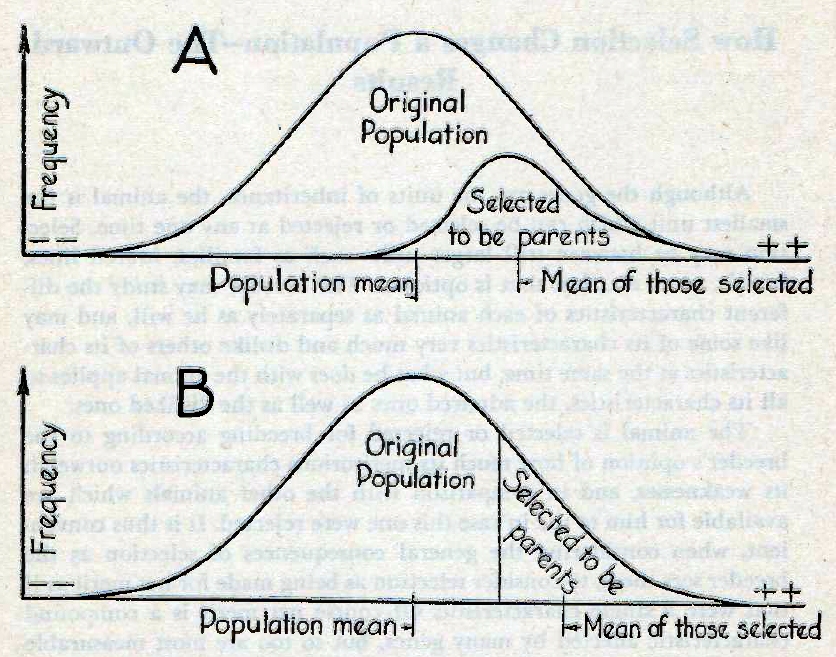
\includegraphics[width=\textwidth]{Figure_17.png}
    \caption{Two ways in which the merits of those chosen to be parents by rather
			 intense selection might be distributed with respect to the merit of the original population
			 from which they were taken. The better individuals are to the right, the poorer
			 to the left. A indicates the usual kind of selection where at least a few mistakes are
			 made and where some attention must be paid to characteristics other than the one
			 for which merit is indicated here. B is the most extreme form of selection conceivable.
			 No mistakes are made and selection is entirely for the characteristic for which
			 degrees of merit are indicated along the horizontal scale.}
    \label{fig:Lush_Figure_17}
    \index{Generation interval}
\end{figure}

\section*{THE SELECTION DIFFERENTIAL}
\index{Replacement rates|(}
\index{Selection!differential|(}

The most useful measure of the intensity of the selection actually
practiced is the difference between the average of those selected to be
parents and the average of the whole population in which they were
born. It is convenient to speak of this superiority of the selected parents
as the ``selection differential.'' As a numerical example, if a herd of gilts
in their first litters farrow an average of 8.6 pigs and we select for large
litter size intensely enough that those which are kept for further breeding
averaged 9.5 pigs in the first litters, then the selection differential
for litter size at this particular \index{Culling levels|(}culling was 9.5 minus 8.6 or .9 pig. The
selection differential which can be attained is sharply limited by the fact
that enough offspring must be saved to replace the parents in any breed
stationary in numbers. More than that must be saved in a breed which
is increasing in numbers. Reproductive rates and percentages of deaths
and other losses from controllable and uncontrollable causes differ
among species of farm animals. Table~\ref{tbl:Lush_Table_11} shows what are believed
to be reasonable figures for the usual percentage of offspring which must be
saved for replacement purposes. The vital statistics of farm animals are
not well enough known to make these estimates as accurate as they
should be. Of course, there is some variation in the replacement rates
from year to year and from farm to farm as conditions of health and
management vary.

Table~\ref{tbl:Lush_Table_12} shows for selection such as that pictured in
\textit{B} of Figure~\ref{fig:Lush_Figure_17} how much the parents can
average above the whole population from which they were selected.\footnote{Table~\ref{tbl:Lush_Table_12}
is for a \textit{normally distributed} population. Most animal breeding
populations are nearly enough normal that these figures are sufficiently accurate to be
useful. Where a few arc culled from the long ``tail'' of a distinctly skew curve, the
gain will be more than is indicated in the upper lines of Table~\ref{tbl:Lush_Table_12},
but gains from the heavier culling shown in the bottom line<1 will he less.}
It thus gives \textit{the maximum} selection differential which could be attained in a
whole breed if the percentage of the population which must be saved for replacement
were the only limiting factor. The selection differential in Table~\ref{tbl:Lush_Table_12}
is expressed in terms of standard deviations, so as to be applicable to all kinds of
characteristics.

\begin{table}[htbp]
	\centering
	\caption{\textsc{Estimated Replacement Rates Which Limit Breed\\Improvement}}
	\label{tbl:Lush_Table_11}
	\begin{tabular}{L{2.5cm}|C{3.5cm}|C{2cm}|C{2cm}}
		\hline
		\hline
%		\multirow{5}={Kind of Animal} & \multirow{5}{2.5cm}{Average Interval Between Generations (i.e., Average Age of Parents When Their Offspring Are Born)} & \multicolumn{2}{C{6cm}}{\multirow{4}={Percentage of Progeny Reared Which Are Needed for Replacements in a Population Static Numbers}} \\
		& Average Interval &
		\multicolumn{2}{C{5cm}}{ } \\
		& Between &
		\multicolumn{2}{C{5cm}}{ } \\
		& Generations &
		\multicolumn{2}{C{5cm}}{Percentage of Progeny} \\
		& (i.e., Average & 
		\multicolumn{2}{C{5cm}}{Reared Which Are} \\
		& Age of Parents &
		\multicolumn{2}{C{5cm}}{Needed for Replacements} \\
		& When Their &
		\multicolumn{2}{C{5cm}}{in a Population} \\
		& Offspringx &
		\multicolumn{2}{C{5cm}}{Static in Numbers} \\
		\cline{3-4}
		Kind of Animal	& Are Born)	& Females	&	Males \\
		\hline
		Horses			& 9 to 13 years					& 35 to 45	& 2 to 4	\\
		Beef cattle		& 4\nicefrac{1}{2} to 5 years	& 40 to 50	& 3 to 5	\\
		Dairy cattle	& 4 to 4\nicefrac{1}{2} years	& 50 to 65	& 4 to 6	\\
		Sheep			& 4 to 4\nicefrac{1}{2} years	& 45 to 55	& 2 to 4	\\
		Swine			& About 2\nicefrac{1}{2} years	& 10 to 15	& 1 to 2	\\
		Chickens		& About 1\nicefrac{1}{2} years	& 10 to 15	& \nicefrac{1}{2} to 2	\\
		\hline
	\end{tabular}
\end{table}

An example will show how Tables~\ref{tbl:Lush_Table_11} and \ref{tbl:Lush_Table_12} are used. The standard
deviation of the weights of fleeces shorn in the same year from a group
of Rambouillet sheep described in Technical Bulletin 85 of the United
States Department of Agriculture is about l.86 lbs. (See Table 2 in that
bulletin.) If a hitherto unculled group of such ewes and rams were to be
culled solely on fleece weight at a single shearing, the 50 per cent of the
ewes which it would be necessary to save would excel the flock average
by .80 times the standard deviation, or 1.49 pounds of wool. The 3 per
cent of the rams with the heaviest fleeces would excel the average for
all rams by 2.27 times the standard deviation, or 4.22 pounds of wool.
Since inheritance is practically equal from sire and dam, this would
make a selection differential of 2.86 pounds of wool at that one shearing,
so far as the next generation is concerned.
\noclub[3]
\index{Replacement rates|)}

\section*{INCREASE TO BE EXPECTED IN THE POPULATION MEAN}
\index{Environment and heredity|(}

The next generation would be expected to be about as variable as
the preceding one, but to average outwardly whatever their parents
averaged genetically. In case the genes all combined their effects additively
and the existing environmental variations did not affect the characteristic
at all, the genetic average of the parents would be the same as
their phenotypic average, the offspring would average whatever their
selected parents did, and the increase in the population mean per generation
would be equal to the selection differential (see Figure~\ref{fig:Lush_Figure_18}).
Actually the permanent improvement in the population average each
generation will be only a fraction of the selection differential.
\index{Additive effects of genes} That fraction
has for its numerator the additively genetic variance (Chapter 7)
and for its denominator the actual variance\index{Variance}; i.e., the fraction is
$\frac{\sigma_G^2}{\sigma_G^2 + \sigma_D^2 + \sigma_I^2 + \sigma_E^2}$ which for
brevity we may call the \index{Heritability|(}``heritability'' of the differences which existed in the
parental generation before selection began. In addition, \index{Epistatic effects|(}
epistatic differences
will cause temporary gains which in amount are less than half of
$\frac{\sigma_I^2}{\sigma_G^2 + \sigma_D^2 + \sigma_I^2 + \sigma_E^2}$ of the
selection differential. These gains from selecting for epistatic differences
tend to disappear in future generations as the genes recombine. They
can be maintained only by continued selection.

\begin{table}
	\centering
	\caption{\textsc{Selection Differential (in Terms of Standard Deviations) Attainable by Various Intensities of Selection}}
	\label{tbl:Lush_Table_12}
	\begin{tabular}{C{5cm}|C{5cm}}
		\hline
		\hline
		Percentage of Population Saved	& Selection Differential 	\\
		\hline
		.90								& .20						\\
		.80								& .35						\\
		.70								& .50						\\
		.60								& .64						\\
		.50								& .80						\\
		.40								& .97						\\
		.30								& 1.16						\\
		.20								& 1.40						\\
		.10								& 1.75						\\
		.05								& 2.06						\\
		.04								& 2.15						\\
		.03								& 2.27						\\
		.02								& 2.42						\\
		.01								& 2.67						\\
		\hline
	\end{tabular}
\end{table}

In the example of selection concentrated on fleece weight, the
increase in average fleece weight per generation would be 2.86 pounds
per generation in the impossibly extreme case in which all differences in
the parental generation were additively genetic, 1.43 pounds per generation
in case heritability of differences is 50 per cent, and only .95
pounds per generation in the more probable case that heritability of
differences in shearing weights is about one-third. The annual increa se
in the flock average would be about one -fourth or fifth of these increases
\textit{per generation}, since the interval between generations, the average age
of the parents when the lambs are born, is about four or five years.
\index{Selection!differential|)}

This example is somewhat artificial for farm animals in that it
assumes that all selection would be practiced at one stage in each generation.
Actually, only a few of the rams born would be kept as rams
even until the first shearing. Many of the ewes would be culled after the
second shearing, others would be culled after the third shearing, others
after the fourth, etc., some culling taking place all through the lifetime
of that band of sheep and much of the culling being based on things
other than fleece weight. All these things operate to lessen the intensity
of the culling which could be done at any one time and to render difficult
the measurement of the intensity of the selection actually practiced.
The example illustrates the general principles that the intensity
of selection possible is sharply limited by the necessity for replacements
and that the intensity of selection actually practiced is to be measured
in terms of the difference between the average of those saved for parents
and the average of the generation in which they were born. The
method of computing the selection differential in this example is fairly
well suited in actual practice to the case of an animal, or some of the
annual plants, where the generations do not overlap and where nearly
all the selection is practiced at one stage in the life cycle.
\index{Culling levels|)}
\nowidow

\section*{CONSEQUENCES OF INCOMPLETE HERITABILITY}

Some individuals are mistakenly saved or rejected for parents
because the effects of environmental variations make them appear
phenotypically better or worse than their genetic values. These environmental
effects are not transmitted to their offspring. Selection of the
phenotypically superior tends automatically to keep among those
saved more than a fair share of lhose which appeared phenotypically
better and less than a fair share of those which appeared phenotypically
worse than they were genetically. The environmental effects are left
behind when they reproduce. Their genes segregate from these combinations
to recombine in the unselected offspring to give a nearly fair
picture of the genetic worth of the parents.

Similarly where the favorable genes tend to be dominant the heterozygotes
will have been made to appear phenotypically better and the
homozygotes relatively worse than corresponds to their average breeding
value. The \index{Dominance}dominance deviations of a parent are not transmitted as
such to its offspring, since they are caused by the interaction of a pair
of allelic genes and only one gene out of each allelic pair can be transmitted
in any one gamete.

Epistatic effects, being dependent on combinations of nonallelic
genes, are transmitted to a portion of the offspring, that portion being
progressively smaller the more complex the combination. If \textit{A} and \textit{B}
are not linked but together have an effect which neither of them has
separately, that effect would be transmitted in about one-fourth of the
gametes from an \textit{AaBb} individual, whereas the additive effects of \textit{A}
would be transmitted in about half of the gametes. An epistatic effect
requiring the joint presence of three nonlinked genes, \textit{A}, \textit{B}, and \textit{C},
would be transmitted in only about one-eighth of the gametes from an
AaBbCc individual, etc. Even when such epistatic effects are transmitted,
the gene combinations responsible for them tend to segregate in
later generations, this process tending to continue until the genes are
combined at random. Hence the partial but transitory gains from selecting
for epistatic differences.

Figure~\ref{fig:Lush_Figure_18} shows what would be expected to happen in an experiment
on selecting for a perfectly hereditary character, with the selection
intensity such that in the high line only the upper half in each generation
were saved for parents, while in the low line only the lower half in
each generation were saved for parents. Obviously, even with such an
impossibly extreme case as perfect heritability (no effects at all by
environment, dominance, or epistasis), it will require several generations of
selection before all overlapping between the two lines ceases. Among
the offspring of selected parents there will always be some poorer than
the poorest of the parents although, if heritability were perfect, the
average of the offspring would equal the average of their selected
parents. The selected parents will not be much more or less homozygous
than the average of the population from which they came. They will
produce some gametes worse than are typical of them as well as some
which are better. When two inferior gametes unite, the result is an offspring
poorer than the poorest of those individuals which were saved to
be parents.

\begin{figure}
	\centering
    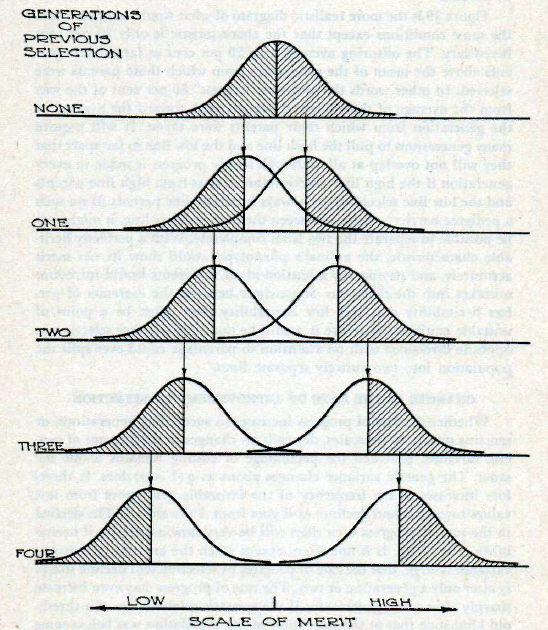
\includegraphics[width=\textwidth]{Figure_18.png}
    \caption{The results expected when selecting simultaneously a high and a low
			 line for a perfectly hereditary characteristic. In the high line the high half and in
			 the low line the low half in each generat1on are saved as parents.}
    \label{fig:Lush_Figure_18}
\end{figure}

Figure~\ref{fig:Lush_Figure_19} is the more realistic diagram of what would happen under
the same conditions except that the characteristic is only 20 per cent
hereditary. The ofhpring average only 20 per cent as far as their parents
above the mean of the generation from which those parents were
selected. In other words the offspring ``regress''\index{Regression|(} 80 per cent of the way
from the average of their selected parents back toward the average of
the generation from which their parents were taken. It will require
many generations to pull the high line and the low line so far apart that
they will not overlap at all, although steady progress is made in every
generation if the high line selections are always from high line parents
and the low line selections are always from low line parents. If no such
a pedigree barrier were put between the high and low line, it might not
be possible to separate the two lines completely. With a perfectly heritable
characteristic, the animal's phenotype would show its net merit
accurately, and paying any attention at all to parents would introduce
mistakes into the selections. Somewhere between the extremes of perfect
heritability and very low heritability there must be a point of
unstable equilibrium where it would be doubtful whether selection in
opposite directions with no attention to parentage could ever split the
population into two entirely separate lines.

\begin{figure}
	\centering
    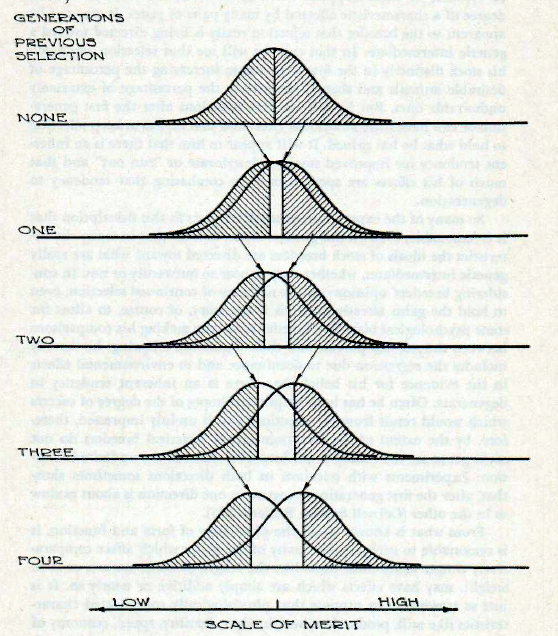
\includegraphics[width=\textwidth]{Figure_19.png}
    \caption{The results expected when selecting simultaneously a low line and a
			 high line for a characteristic only 20 per cent hereditary. Selection is entirelv on the
			 individual's own characteristics except that its parents must have belonged to the
			 same line it did; i.e., there is a pedigree barrier against exchanging animals from one
			 line to the other, no matter what their individual characteristics are. The intensity of
			 selection is such that in each line half are saved to be parents.}
    \label{fig:Lush_Figure_19}
\end{figure}
\index{Environment and heredity|)}
\index{Heritability|)}

\section*{CHANGES IN THE RATE OF IMPROVEMENT BY SELECTION}
\index{Variation!as affected by selection|(}

Whether the rate of progress increases in succeeding generations, or
remains steady, or decreases, depends on changes in the amount of genetic
variance, provided the percentage of culling remains about the
same. The genetic variance changes about as $q(l - q)$ does. It therefore
increases as the frequency of the favorable genes goes from low
values toward .5 and declines as it goes from .5 toward 1.0. The decline
in the rate of progress even then will be very slow, especially if heritability
is not high. It is not often , except when the amount of epistatic
variance is large, that the rate of progress by selection will decline sharply
after only a generation or two. The rate of progress may even increase
sharply after a few generations if the epistatic relations are of a threshold
kind such that at the start most of the population was below some
threshold above which it must rise before the genetic differences could
express themselves freely. Something of this kind seems to have happened
in Payne's selection experiments for bristle number in Drosophila
(Indiana University Studies V, No. 36. 1918) and perhaps in Goodale's
selection for body weight in mice (\textit{Journal of Heredity} 29: 101--12,
1938.)
\index{Variation!as affected by selection|)}

\section*{SELECTION FOR EPISTATIC EFFECTS}
\index{Selection!for epistatic effects|(}

The kinds of gene interaction possible are so numerous that they
defy cataloguing, but the outward results of selecting for them seem to
be typified by what happens when selection favors an intermediate
degree of a characteristic affected by many pairs of genes. It may not be
apparent to the breeder that selection really is being directed toward a
genetic intermediate. In that case he will see that selection improved
his stock distinctly in the first generation, increasing the percentage of
desirable animals and sharply decreasing the percentage of extremely
undesirable ones. But he will see that selections after the first generation
or two have little additional effect and that he has to keep selecting
to hold what he has gained. It will appear to him that there is an inherent
tendency for improved stock to deteriorate or ``run out'' and that
much of his efforts are spent merely in combating that tendency to
degeneration.

So many of the experiences of stock breeders fit this description that
it is reasonable, even on this ground alone, to infer that in many characteristics
the ideals of stock breeders are directed toward what are really
genetic intermediates, whether they appear so outwardly or not. In considering
breeders' opinions on the necessity of continued selection, even
to hold the gains already made, it is necessary, of course, to allow for
some psychological bias. The breeder is usually making his comparisons
between the \textit{selected} parents and their \textit{unselected} offspring; he thereby
includes the regression due to dominance and to environmental effects
in the evidence for his belief that there is an inherent tendency to
degenerate. Often he has built unjustified hopes of the degree of success
which would result from his selections and is unduly impressed, therefore,
by the extent of his disappointments. Practical breeders do not
often get to see the results of deliberate selection in the undesired direction.
Experiments with selection in both directions sometimes show
that, after the first generation, progress in one direction is about as slow
as in the other (Cornell Station Bulletin 533).

From what is known about the physiology of form and function, it
is reasonable to suppose that many of the genes which affect comparatively
simple anatomical traits like the length of bone, stature, or even
weight, may have effects which are simply additive or nearly so. It is
just as reasonable to suppose that physiologically complicated characteristics
like milk production, health, vigor, fertility, speed, economy of
gain, etc., are dependent for their maximum expression on a harmonious
balancing of the magnitudes and functions of many different
organs. If that is so, then it must often happen that in selecting for
maximum production in these economically important characteristics
the breeder really is selecting for balanced or intermediate sizes of
lungs, of heart, of digestive tract, etc. As a purely mechanical illustration,
consider how with an automobile the maximum mileage per gallon
of gasoline is not obtained at the very slowest speeds and certainly
not at the very highest speeds. Moreover the value of the driver's time
or the urgency of the errand may make the most desirable speed something
other than that which is most economical of gasoline. In most
stock judging there is much emphasis on symmetry and ``balance'' in
the animal as a whole. Perhaps this is more justified than would be the
case if each gene were consistently desirable or consistently undesirable,
as is inferred in many discussions of applied genetics.

\index{Selection!for intermediate|(}
A good example of a characteristic which is optimum at an intermediate
value is the thickness of the back fat in hog carcasses to be sold
in the bacon trade. In Sweden since 1938 the optimum thickness of fat
over the middle of the back has been considered to be 29 to 31 mm.\footnote{For
details sec: Activities of the research statiom for testing swine breeding
stock during 1937 (Translated title), Bui. 487 from "Centralanstalten f\"or
f\"ors\"oksv\"asendet p{\aa} Jordbruksomr{\aa}det" Stockholm, 1938.}
When the thickness is already near this optimum, an increase or
decrease of one millimeter changes the carcass value only a little. But
when the fat is already extremely thin, or much too thick, then one
more or one less millimeter in thickness makes a large change in the
value of the carcass. For example, an increase of one millimeter would
change the carcass score as follows when the initial thickness is as
shown:

\begin{table}[h]
	\centering
	\begin{tabular}{cc}
	Initial thickness		& Change in score \\
	13 mm.					& 3.5 points increase \\
	19 mm.					& 2.2 points increase \\
	27 mm.					& .5 points increase \\
	33 mm.					& .6 points decrease \\
	36 mm.					& 1.3 points decrease \\
	44 mm.					& 3.1 points decrease \\
	\end{tabular}
\end{table}

\noindent
Thus a gene which will increase backfat thickness one millimeter
would be highly desirable in a population where the carcasses range
between 14 and 22 millimeters in thickness. Most of its effects in that
population would be additive and selection for the relatives of those
which have the best carcasses would increase the frequency of that gene.
In a population which averages 30 mm. in thickness such a gene would
lower desirability of its possessor in about as many cases as it would
increase desirability. Its average effect would be zero, all of the individual
effects it actually makes would be epistatic, and selection would
not tend consistently either to increase or decrease its frequency. In a
population in which the thickness already ranges from 36 to 44 mm.,
such a gene would be undesirable, nearly all of its effects would be additive,
and selection would tend to lower its frequency.

The emphasis laid on symmetry, balance and proportion in most
animal husbandry judging, the physiological and mechanical relations
between the functioning of an animal and the dimensions of its parts,
the fact that so many chemical reactions in metabolism are of a threshold
nature, and similar considerations, indicate that situations in which
the intermediate is favored over either extreme are rather common,
although there may be some strictly linear relations, too. Probably
there are many situations in which the regression of desirability on
genotype is curvilinear but the curvature is slight enough within the
limits of that population that a straight line comes fairly close to
describing the facts and selection would change gene frequency a long
way before reaching an optimum or some threshold beyond which
further changes in gene frequency would have no effect on average outward
desirability.

\index{Equilibrium between selection and mutation!when selecting for an intermediate|(}
The idea of a desirable intermediate may be extended, and indeed
must be extended, to cover cases where two or more intermediates
widely separated on the genetic scale may each be more desirable than
the genotypes immediately adjacent to them and yet need not be exactly
equal in their own desirability. Desirability for the purposes of the
animal breeder (or ``fitness,'' if the problem is being considered from
the evolutionary point of view) is such a complex thing that there must
be many cases where a certain magnitude of a characteristic fits its possessor
better for a certain purpose than magnitudes just a little larger or
a little smaller would, and yet a magnitude very distinctly larger or
smaller would fit it better for some other purpose or ecological niche.
A crude illustration of that is milk production in cattle. There are
regions, especially in the corn belt, where both specialized beef production
and specialized dairy production can be profitable systems of farming.
The most desirable milk production for a cow used in the
specialized beef farming is just enough to feed her calf well. More than
that would lead to some trouble with spoiled udders, etc. But the peak
of desirability in specialized dairy production is far different. There
may, of course, be other farms where the physical resources and the
aptitudes of the owner make an intermediate milk production most
desirable. In that case there might exist, even in the same region, several
different peaks of desirability in milk production. Another example is
size in horses. In most of the United States there is not much demand
for a horse which is too big to be a children's pony but too small to be a
good saddle horse for a grown person. If it were small enough (like the
Shetlands) or large enough (like the American Saddle Horse), it might
have a high cash value; but, if it is one of the ``in-between'' kinds, there
may be few who will want it. Again, if it were between the ideal for
saddle horses used for pleasure and the ideal for cavalry horses, or if it
were too big for a cavalry horse, it would be at a disadvantage compared
with those which were just the right size. Figure~\ref{fig:Lush_Figure_20} shows such a
situation diagrammatically, so far as it can be pictured for variation
along one dimension.

\begin{figure}
	\centering
    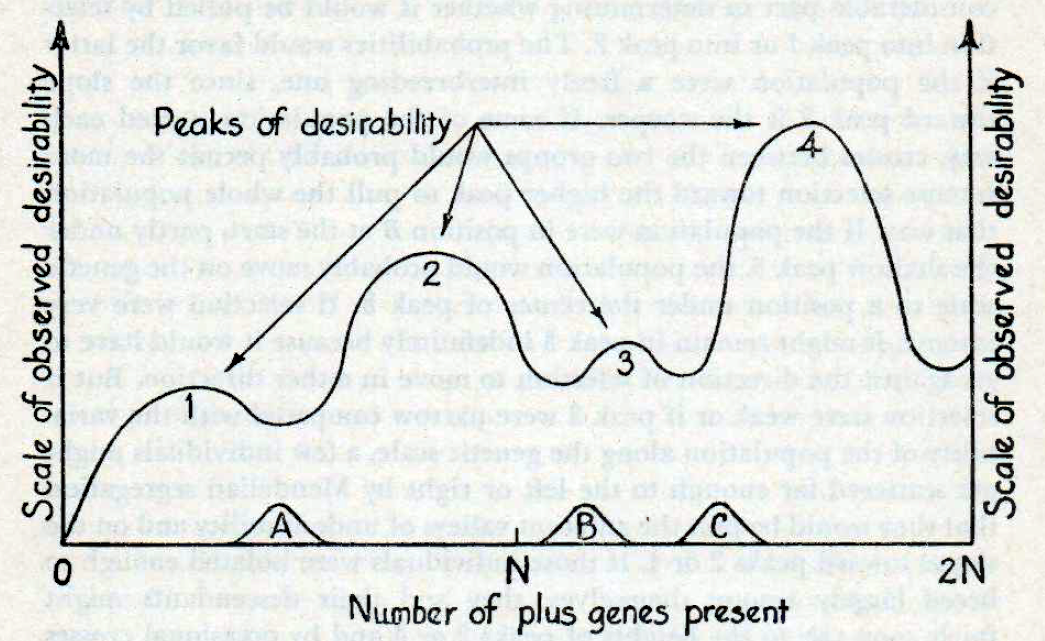
\includegraphics[width=\textwidth]{Figure_20.png}
    \caption{Illustrating the case of several different genetic intermediates (l, 2, 3.
			 and 4), each of which is more desirable than the genotypes which are most nearly like
			 it. \textit{A}, \textit{B}, and \textit{C} are populations whose averages are at 
			 different places along the genetic scale.}
    \label{fig:Lush_Figure_20}
\end{figure}

If the animal's position on the horizontal scale can be seen or measured,
the situation offers no new complications over the general case
already described for selection directed toward an intermediate. But if
only its position on the vertical scale of outward desirability can be
observed\footnote{Thus, in the example about length of leg and speed in race horses, one might
have abundant records on the actual racing speed of many horses but no information
at all about the lengths of their legs. Then one would know in detail whether they
were fast or slow (their outward desirability) but would know nothing about whether
their legs were long or short (their position on the horizontal scale). Two horses
might be equally slow, one because its legs were too short and the other because its
legs were too long, but a man knowing only the record of speed would not know
whether they were alike or far apart on the genetic scale} and the horizontal scale
is long enough for the peaks of desirability to be distinctly separated from each
other by deep valleys, then a new kind of complexity occurs. That is shown by \textit{A}, \textit{B}, and \textit{C},
which represent different positions along the genetic scale in which the
genotypes of a population might happen to be distributed when selection
began. If a population were in position \textit{A}, immediately in the valley
of undesirability between peaks 1 and 2, chance would play a
considerable part in determining whether it would be pulled by selection
into peak 1 or into peak 2. The probabilities would favor the latter
if the population were a freely interbreeding one, since the slope
toward peak 2 is the steeper. If some of the population started each
way, crosses between the two groups would probably permit the more
intense selection toward the higher peak to pull the whole population
that way. If the population were in position \textit{B} at the start, partly under
the shallow peak 3, the population would probably move on the genetic
scale to a position under the center of peak 3. If selection were very
intense, it might remain in peak 3 indefinitely because it would have to
go again st the direction of selection to move in either direction. But if
selection were weak or if peak 3 were narrow compared with the variability
of the population along the genetic scale, a few individuals might
get scattered far enough to the left or right by Mendelian segregation
that they would be past the adjacent valleys of undesirability and on the
slopes toward peaks 2 or 4. If those individuals were isolated enough to
breed largely among themselves, they and their descendants might
fairly soon rise to the heights of peaks 2 or 4 and by occasional crosses
back with the rest of the population might pull the whole population
over to their peak. If, however, the occasional individuals which are
different from their population in enough genes to be past the valleys
interbred freely with the whole population, their offspring would probably
be pulled back into the general population because the mates
would usually be near the population average.
\index{Equilibrium between selection and mutation!when selecting for an intermediate|)}

Whether the population would remain in peak 3 would therefore
depend on the balance between selection, the degree to which the population
tends to separate into rarely interbreeding groups, and the height
and width of peak 3 and the depths of the valleys surrounding it. The
more intense the selection, the more the population would tend to be
held in that peak. The only force tending actively to get it out of that
peak to where it might perhaps find the road to a higher peak is chance
at segregation causing gene frequency to vary in a random direction.
That is a very weak force in large freely interbreeding populations but
may become powerful in a population highly subdivided into small
groups which rarely interbreed. This latter condition leads to some
mild inbreeding which, under some circumstances, may be necessary to
get a population out of a peak where selection has carried it. If the
population were at position \textit{C} when selection began, selection would be
almost certain to carry it to peak 4. There would be no need of inbreeding
to help in that.

This may explain some of the surprising effects sometimes observed
when crossing distinct strains or races. Crossing race \textit{A} and \textit{B} would
give a population with gene frequencies putting it nearly in the center
of peak 2 and would be considered a ``lucky nick .'' On the other hand,
crossing a race already in peak 2 with one already in peak 4 would give
a race with gene frequencies which would put it near the much lower
peak 3. The unfavorable effect might not show in the first generation of
the cross, since each race contributes a full set of its genes, and there is
often enough dominance of the favorable genes to furnish a margin of
safety. But if the first crosses were interbred, the decline in merit from
$F_1$ to $F_2$, when the combinations of genes which worked well together
were scattered, might be extreme. How often this actually happens is
open to question but it points toward a general principle, valid when
epistatic effects are important, that in attempting to perpetuate the
good qualities of an individual it should be mated to members of the
same race or local strain rather than to equally good individuals from
unrelated races where the gene frequencies and combinations may be
widely different. This is the principle of ``linebreeding'' (\textit{\textbf{Chapter 23}}).
Crosses with unrelated or distantly related races may sometimes be
advantageous, too, in originating new lines with desirable combinations
but should always be considered experimental and venturesome, rather
than a dependable general practice.

Desirability for the purposes of the breeder, or fitness in terms of
evolution, depends on many different characteristics, each of which
may have intermediate peaks of desirability. The interdependence of
these on each other's magnitudes increases tremendously the possibilities
for such peaks of desirability where all adjacent genotypes which
might be reached easily by Mendelian segregation in a freely interbreeding
population are less desirable. Figure~\ref{fig:Lush_Figure_20} is a rough sketch of
that, showing variability in only one characteristic. Figure 21 shows the
interplay of variation in two dimensions on desirability, ·which is pictured
as the height of an irregular surface. By observing the increased
complexity of Figure~\ref{fig:Lush_Figure_21} over that of Figure~\ref{fig:Lush_Figure_20}, one can imagine how
complex the situation may be in reality where adaptation or desirability
depends on variation in \textit{n} dimensions and \textit{n} is a large number!

While it appears impossible ever to know enough about the genes
and their physiology and their interplay with environmental circumstances
to know a population's position exactly in all n dimensions of its
adaptability, or to explore the surrounding terrain clearly enough to
know whether there is a higher peak of desirability nearby which might
be reached, yet the general consequences of selection in such a situation
are fairly clear. Selection when first applied will quickly (in terms of
generations) carry the population up the steepest slope of increasing
desirability to the nearest peak in that direction. Selection cannot carry
the population across a deep intervening valley of lessened desirability
to reach a peak of higher desirability on the other side. Only chance
wandering of gene frequency against selection can do that, and this
chance wandering is a very feeble force except when there is considerable
inbreeding. The terrain is apt to be extremely rugged and irregular
in places where two or more genes which individually have very
minor effects may in certain combinations have extremely important
effects on desirability. This gives rise to surprising ``nicking'' effects
which can hardly be seized by selection alone if they are dependent on
more than three or four genes which separately have undesirable effects.

\begin{figure}
	\centering
    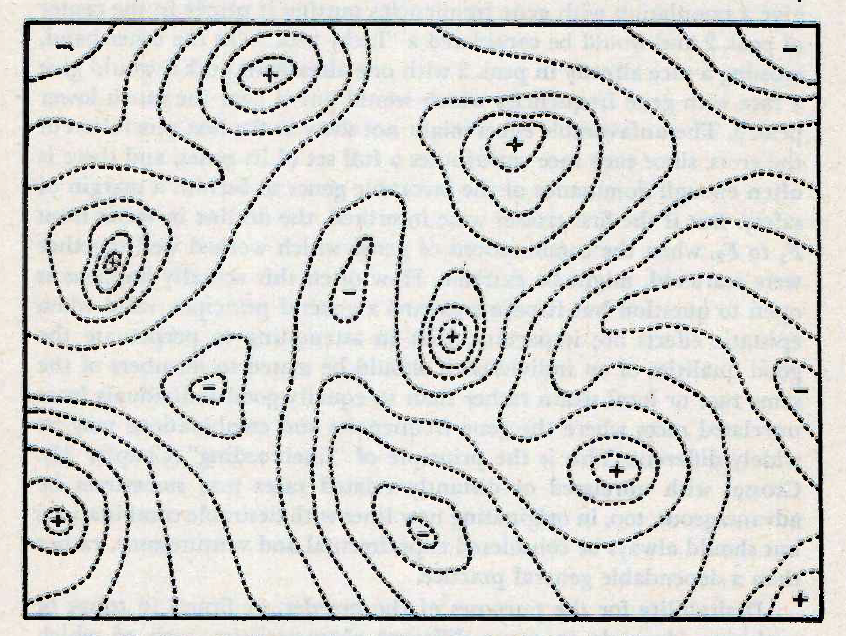
\includegraphics[width=\textwidth]{Figure_21.png}
    \caption{Contour diagram showing how the level of desirability may depend on
			 genetic variability in two different characteristics. Plus signs indicate peaks, and
             minus signs indicate hollows. Selection can carry a population up a slope of c  ontinuously
             increasing desirability but cannot carry it down a slope and across an intervening
             valley to reach a still higher peak (After Wright in \textit{Proc. Sixth Intenat.
             Cong. Genetics}).}
    \label{fig:Lush_Figure_21}
\end{figure}

As a result of the power of selection to carry populations into these
peaks and its inability to get the population out again, most characteristics
which have been under selection for many generations may be
expected already to be in some of those peaks. It is only when selection
in a new direction is just beginning that the position of the population
is as apt to be on a slope ready for rapid progress as it is to be in a peak.
As ideals change with economic or other conditions, peaks will sometimes
change to valleys or the reverse, thus releasing the population
from its peak and permitting rapid progress in some new direction for a
time. To some extent this surface of desirability is always changing, like
that of the sea, so that the peaks do not remain peaks forever. Yet the
rate of such change may perhaps be so slow that, except for changes in
ideals which are caused by changes in economic conditions, it should be
likened more fairly to geological changes in the heights of mountains
and plains.
\index{Epistatic effects|)}
\index{Selection!for epistatic effects|)}
\index{Selection!for intermediate|)}

\section*{SELECTION FOR MANY CHARACTERISTICS AT ONCE}
\index{Scoring|(}
\index{Selection!indexes|(}
\index{Selection!tandem method|(}

The practical animal breeder must consider many different characteristics
in his selections. Some of these are independent of each other
or nearly so; others are positively correlated so that selection for one of
them brings with it a little improvement in the other, although, even if
\textit{x} and \textit{y} are correlated rather closely, selection for \textit{x} indirectly by
selecting for \textit{y} is less effective than selecting for \textit{x} directly if that is possible.
Others are negatively correlated with each other. This makes it a little
harder to select for both of them at once than it would be if they were
independent. Some characteristics are much more important than others.
This needs to be taken into account in balancing excellencies in one
respect against deficiencies in other respects when deciding whether to
keep or cull the animal. The fact that several things must be considered
lowers the intensity of selection possible for each of them, but there is
no escape from that so long as all those things have something to do
with the net desirability of the animal to the breeder or to his
customers.

\index{Culling levels|(}Culling may be done in at least three general ways. The first or tandem
method is to select for one characteristic at a time until that is
improved, then for a second characteristic, later for a third, etc., until
finally each has been improved to the desired level. The second method
is to cull simultaneously but independently for each of the characteristics.
This amounts to establishing for each characteristic culling levels,
below which all individuals are culled, no matter how good are in
other characteristics. The third method is to establish some kind of a
total score or selection index to measure net merit. This would be done
by adding The animal's score for its merit in \textit{x} to its scores for merit in \textit{y},
in \textit{z}, etc. Then those with the poorest total scores would be culled.
Figure~\ref{fig:Lush_Figure_22} illustrates the total score method where two characteristics are
involved.

The tandem method is by far the least efficient of the three, even
when the characteristics are not affected by any of the same genes and it
can be assumed that the improvement made in the first one will not
be lost later while selecting for improvement in the others. Selecting for
one thing at a time will improve that one thing faster than can be done
by any other method of selection, but while that is being done the other
things must wait. Where other things must be improved also, the
improvement made in the first characteristic while it was under selection
must be divided by the whole number of generations necessary to
improve them all in order to get the average rate of improvement in
that one thing. In the simple case in which n characteristics are independent
and equally important, the average improvement per generation
in each will be only one nth of the improvement which is made in
it in the generations when it is the sole object of selection. In this case
the selection index method is $\sqrt{n}$ times as efficient as the tandem
method.

The selection index method is more effective than the method of
independent culling levels because it permits unusually high merit in
one characteristic to make up for slight deficiencies in the other. When
culling by the total score method under the simple conditions of \textit{n} independent
and equally important characteristics, selection for each characteristic
will be $\frac{1}{\sqrt{n}}$ as intense as if all the efforts of selection could
have been concentrated on that characteristic alone.

Under the method of independent culling levels, if \textit{w} is the fraction
of the population which must be saved for breeding, then the intensity
of selection for each characteristic is the same as if selection were directed
at that alone but the fraction which must be saved were $\sqrt[n]{w}$. For
example, if length of body and soundness of feet and legs are uncorrelated
in swine, and a breeder must save 10 per cent of his gilts for breeding
purposes, he can save the 10 per cent with the very longest bodies if
he selects for that alone, or the 10 per cent with the soundest feet and
legs if he selects for that alone, but only 1 per cent of his gilts will be in
the best 10 per cent in both respects. If he pays equal attention to both
things, he must save all gilts which are in the 32 per cent which are
longest and are also in the 32 per cent with best feet and legs if he is to
save IO per cent of his gilts altogether. If he takes quality also into
account, and if quality is not correlated with body length or with
excellence of feet and legs, he will have to save from among the best 46 per
cent (instead of 32 per cent) in each trait in order to have IO per cent of
the best in all three respects. Four traits would increase this to 56 per
cent instead of 46 per cent. If the traits are positively correlated with
each other, the intensity of selection for single traits will not fall off
quite so fast with increasing \textit{n} as these formulas indicate; but, if the
traits are negatively correlated, the intensity of selection for each will
fall off a little faster.

\begin{figure}
	\centering
    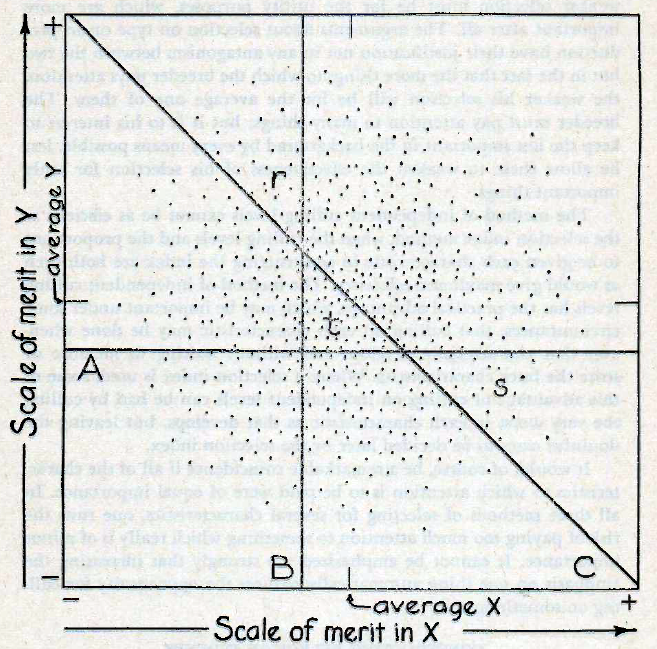
\includegraphics[width=\textwidth]{Figure_22.png}
    \caption{Superiority of culling on total score as compared with culling independently
			 first for one characteristic and then for another. Each dot represents an individual.
			 Merit in \textit{x} is not correlated with merit in \textit{y}. \textit{A} represents the level of merit
			 in characteristic \textit{y} below which all individuals are culled when \textit{y} is considered
			 independently. Similarly, \textit{B} represents the independent culling level for merit in \textit{x},
			 all individuals to the left of \textit{B} being culled. \textit{C} represents a level of culling on total
			 score, with \textit{x} and \textit{y} being regarded as equally important, which would result in keeping
			 an equal fraction of the population. Animals in areas \textit{r} and \textit{s} would be kept when
			 culling on total score but would be discarded when culling independently on \textit{x} and
			 \textit{y}, while the reverse would be true of the animals in area \textit{t}. The fate of the animals
			 in the other four areas would not be altered by changing the method of culling. If \textit{x}
			 and \textit{y} were not equally important the example is still valid, but the slope of line \textit{C}
			 would be different (Brier \textit{et al.}, pages 153--60, in \textit{Proc. Amer. Soc. An. Prod.} for 1940}
    \label{fig:Lush_Figure_22}
    \index{Selection!tandem method|)}
\end{figure}

Here lies the real damage done by paying attention to \index{``Fancy points''}``fancy
points'' in selection; namely, that the more attention given to them, the
weaker selection must be for the utility purposes, which are more
important after all. The arguments about selection on type or on production
have their justification not in any antagonism between the two
but in the fact that the more things to which the breeder pays attention,
the weaker his selection will be for the average one of them. The
breeder must pay attention to many things; but it is to his interest to
keep the less important in the background by every means possible, lest
he allow these to weaken the effectiveness of his selection for truly
important things.

The method of independent culling levels cannot be as efficient as
the selection index method, when the culling levels and the proportions
to be given each characteristic in constructing the index are both such
as would give maximum efficiency. The method of independent culling
levels has the practical advantage, which may be important under some
circumstances, that culling on each characteristic may be done whenever
that characteristic develops and without waiting to measure or
score the later characteristics. Where a selection index is used, some of
this advantage of culling on independent levels can be had by culling
the very worst in each characteristic as that develops, but leaving the
doubtful cases to be decided later by the selection index.

It would, of course, be a remarkable coincidence if all of the characteristics
to which attention is to be paid were of equal importance. In
all three methods of selecting for several characteristics, one runs the
risk of paying too much attention to something which really is of minor
importance. It cannot be emphasized too strongly that increasing the
emphasis on one thing automatically reduces the opportunity for culling
on something else.
\index{Culling levels|)}
\index{Scoring|)}

\section*{CONSTRUCTING SELECTION INDEXES}
\index{Heritability|(}
\index{Heritability!methods of estimating}

The principles of constructing selection indexes designed to make
maximum improvement, are those of multiple regression where it is
desired to predict as accurately as possible an unknown or ``dependent''
variable from two or more known (independent) variables. In this case
the dependent variable is the animal's net genetic merit or breeding
value, while its various characteristics or even the characteristics of its
relatives are the independent variables.

Four bits of information are needed for each characteristic. 1. The
average amount which a given variation in that characteristic actually
raises or lowers the net phenotypic merit of the animal. This we may
call the \textit{importance} of the characteristic. 2. The \textit{heritability} of each
characteristic is important because it is the average fraction of phenotypic
improvement we get in the offspring for each unit of phenotypic
merit in the selected parent. 3. \textit{Genetic correlations} between that 
characteristic and the others may arise if some of the same genes affect two
or more of them. These will mean that selection for characteristic \textit{x} will
help or hinder improvement in characteristic \textit{y}, as compared with what
would happen if they were independent. 4. \textit{Phenotypic correlations}
between that characteristic and the others will exist if some of the same
environmental incidents have affected them. This, in combination with
differences in heritability, may even lead to some characteristics being
useful mainly as indicators of the kind of environment under which
more important characteristics developed.

A quantitative example of the idea of relative importance is the
finding by Winters (\textit{The Empire Jour. of Exp. Agr.} 8:259--68, 1940)
that one pound of wool is worth 3.4 pounds of lamb. The relative
importance of each characteristic may need to be established separately
for each kind of animal, each region, each type of farming, and almost
for each breeder. Naturally this job is never done permanently but
needs to be reviewed whenever the market demands and premiums
make any large and presumably permanent change. Discussions about
what is ``the right type'' to breed mainly concern the relative importance
of different characteristics, although they have in them something
of the other three bits of information also.

Heritability can be approximated by doubling the intrasire regression
of offspring on their dams. This requires data on several hundred
pairs and is not likely to be within the reach of the individual breeder,
but from his general observations he can get a rough idea of the relative
heritability of two characteristics by observing whether the offspring
generally tend to resemble their parents rather closely or slightly
in each of these.
\index{Heritability|)}

The genetic correlation between two characteristics on the same animal
can be measured by observing a large number of pairs of closely
related animals and correlating characteristic \textit{x} in one member of the
pair with characteristic \textit{y} in the other. This requires large numbers, and
the estimates have high sampling errors. It is the bit of information
most likely to be lacking when an index is to be constructed.

The environmental correlation between two characteristics can be
had by correlating the two characteristics on the same animal and subtracting
their genetic correlation obtained as above.

Occasionally it is profitable to pay more attention to a highly
hereditary characteristic which is of limited economic importance than
to a slightly hereditary one, the variations in which affect the value of
the individual animal more strongly. This is because heritability is the
fraction which one gets of what he reaches for when selecting the parents,
and importance measures the value of that for which he is reaching.
One will have more net profit by getting 50 per cent of something
which is worth 20 cents than by getting 30 per cent of something which
is worth 25 cents! It is a question of deploying the available efforts and
resources so as to secure maximum returns.

Because of this relation between heritability and importance, the
different characteristics in a selection index should be given emphasis
in proportion to their heritability times their importance, rather than
in proportion to either one alone. This will be completely true if the
characteristics are not correlated. If the characteristics have strong
environmental and genetic correlations among themselves, this might
alter the size and could even reverse the signs of the attention to be paid
to each characteristic when constructing a selection index. This is just a
special case of the well-known fact that in a multiple regression equation,
strong correlations among the independent variables can alter
greatly the net regression coefficients from what they would be if all the
independent variables were uncorrelated with each other. Emphasizing
each characteristic in proportion to the product of its heritability and
its importance is as good an approximation to the proper weights as is
possible in most cases.

The few studies yet made seem to indicate that if heritability and
importance are known with rough accuracy, the efficiency of the index
based on them will not be changed much by the intercorrelations
between the variables, although the relative importance and even the
sign of some of the weights may be changed much. As an example in a
swine breeding experiment at the Iowa Agricultural Experiment Station,
a selection index was first constructed using only the importance
of the items and the observed phenotypic correlation between litter
mates. It was: $I = 1/3W + S + P + .303\bar{W} + 1.667\bar{S}$ where
$W$ is weight at 180 days, $S$ is score for market desirability, $P$
is productivity of dam, $\bar{W}$ is average weight and $\bar{S}$ is
an average score of the litter in which the pig was born. L. N. Hazel's
analysis\footnote{\textit{Genetics} 28:476--490. 1945} of the data which
were then collected in the next few years of the experiment indicated
that the most efficient index would have been:

\[I^\prime = .3W - .5S + .5P + .270\bar{W} + .605\bar{S}\]

The coefficients in the two indexes are markedly different, especially in
the reversed sign for the coefficient of $S$, yet the efficiency of $I$ was .364
and that of $I^\prime$ was .404, which is larger, but not greatly so. By efficiency
is meant that progress by selecting exactly according to $I$ would make
progress .364 as fast as could be made by the same percentage of culling
if the genotype of every pig were known exactly.
\index{Selection!indexes|)}

\section*{SUMMARY OF RESULTS EXPECTED FROM MASS SELECTION FOR NET MERIT}

Mass selection is expected to cause the average of each generation
to exceed the average of the preceding generation by an amount ($M$)
which is equal to the heritability fraction $\frac{\sigma_G^2}{\sigma_O^2}$
of the selection differential ($S$), the latter being the average
merit of those selected to be parents minus the average of the whole generation
from which they were taken.

There is also a little deterioration from mutation, but this is too
small to be considered further in problems of animal or plant breeding,
although it may be important in evolutionary considerations.

When selection is first begun there will also be some temporary gain
from epistatic effects. This will be something less than half of
$S \times \frac{\sigma_I^2}{\sigma_G^2 + \sigma_D^2 + \sigma_I^2 + \sigma_E^2}$.
It will tend to disappear with each generation of segregation and recombination
and thus, unless constantly renewed by fresh selection, tends to disappear soon
after selection is relaxed.

The obstacles to rapid progress naturally fall into two groups: (1)
Circumstances or practices which make $S$ small and (2) circumstances
or practices which make $\sigma_G^2$ small or $\sigma_D^2$, $\sigma_I^2$, or
$\sigma_E^2$ large, thereby lowering heritability. Although \textit{M} may
perhaps be small, it will not be zero, provided both $S$ and $\sigma_G^2$
have positive values.

Among things which may make $S$ small are:
\begin{enumerate}[topsep=0pt, partopsep=0pt]
\item Perhaps only a small fraction can be culled. Remedies: Anything
which will improve the health of the herd and reduce deaths from
disease or accident; earlier breeding and quicker rebreeding of females,
and anything else which will increase the number of offspring raised
annually per 100 females.

\item The population may be so uniform that the difference between
those selected and those rejected cannot be large. Remedy: Sometimes
one can change the environment so that genetic differences may express
themselves more fully and be magnified. Outcrossing may help.

\item The breeder may be careless about his cullings or changeable in
his ideals. This makes the selection more like discarding at random or
at least more like the top than the bottom of Figure~\ref{fig:Lush_Figure_17}.
Remedy: More care in deciding on the ideals, more attention to detail, planning the
cullings and selections well in advance of the time when they must
actually be made.

\item The measures or yardsticks of individual merit may not be definite
or simple. This has the same effect as 3. Remedy: Clearer and more
quantitative definition of goals, more systematic scoring, grading or
classifying at regular ages or dates, simple but systematic records of
production where possible.

\item The breeder may be trying to pay attention to too many things
in his selections, thus weakening the intensity of selection for the more
important things. Remedy: Resolutely keeping minor things in the
background, perhaps using a selection index.

\noindent
Among things which make heritability low are:

\item $\sigma_G^2$ may be small. Remedies: An outcross to a relatively unrelated
stock having some desirable characteristics which are absent or
rare in the breeder's own herd may restore genetic variability. Probably
most breeds of farm animals still have enough genetic variability
within them that crossing with other breeds is not necessary for making
a large amount of further improvement. Introducing blood from outside
the breed cannot be done in most breeds under the prevailing
standards of purebreeding, although outcrossing within the breed is
always possible. Inbreeding a population without discarding any of the
lines tends toward doubling $\sigma_G^2$ but puts most of it between lines and
tends to extinguish genetic variance within lines. When the better lines
are selected and the poorer lines are discarded, the genetic variance
then remaining is likely to be smaller than was in the population when
the inbreeding began. Sometimes it may be possible to alter the environment
enough to magnify the outward differences between genetically
different individuals, particularly where thresholds are involved, but it
may be difficult to find the environmental changes which will do that.

\item $\sigma_E^2$ is usually large except for a few characteristics such as colors
and things which are fairly simple anatomically, such as the dimensions
of the bones, shape of head, set of ear, etc. Remedy: Keep the environment
alike for all individuals as far as is economical, correct for the
effects of the more important differences in environment which did
occur, use lifetime averages where those are practicable, and give some
attention to the merits of relatives and progeny.

\item $\sigma_D^2$ may be large. This can be an important obstacle only where
most of the undesired genes are recessives already rare, and in pairs of
genes where the heterozygote is preferred over both homozygotes. Remedy:
Consider the relatives. The collateral ones usually give more help
in this respect than the ancestors do. The progeny are still more
informative, especially if they are inbred.

\item $\sigma_I^2$ may be large. This seems likely to be important only where
the population has already been under selection for many generations.
Remedy: Consider the relatives and progeny. Inbreed enough to form
distinct families, only rarely making crosses between them. Breed within
the family as long as its average merit is good.
\end{enumerate}

These ways of overcoming partially the obstacles to progress by
mass selection will be considered separately in the following chapters.
The purpose of this chapter has been to describe and explain the results
of unaided mass selection. It alters the population mean almost in proportion
to \textit{n} times the amount it changes gene frequency, n being the
number of genes affecting the characteristic.

The rate of improvement per generation may increase or decrease
in later generations but is not likely to change rapidly unless there is a
considerable amount of epistatic interaction.

Only rarely is mass selection completely ineffective, as when selection
is for a heterozygote, when selection has already carried the population
into a stable epistatic peak, or when selection is within an
entirely homozygous line. Often, however, the rate of progress by mass
selection is slow and could be made more rapid by a judicious use of
relatives and progeny or by more careful control or consideration of the
environment.

\section*{REFERENCES}

The classical cases of selection experiments with higher animals are
those of Castle on the hooded pattern in rats, mostly published from
about 1914 to 1920, and Pearl's experiments on selection for high egg
production in the poultry flock at the Maine Station a little earlier. In
plants the Illinois Experiment Station selections for high and low oil
content and for high and low protein content in corn kernels and
Johannsen's selections in Denmark for seed size in beans are famous
among experiments on selection. For brief accounts of these and other
actual experimental studies of selection, see:

\begin{hangparas}{0.5in}{1}%
Babcock. E. B., and Clausen, R. E. 1927. Genetics in relation to agriculture. pp.
221--31 and 538--50.

Castle, W. E. 1930. Genetics and eugenics. pp. 236--45.

Goodale, H. D. 1938. A study of the inheritance of body weight in the albino
mouse by selection. Jour. Heredity 29:101--12.

Sinnott, E. W., and Dunn. L. C. 1925. Prin. of genetics. pp. 339--46.

Winter, F. L. 1929. Mean and variability as affected by continuous selection for
composition in corn. Jour. Agr. Res. 39:451--76.
\end{hangparas}
\index{Selection|)}
\chapter{Aids to Selection --- The Use of Lifetime Averages}
\label{cha:Lush_Chapter_13}
\index{Lifetime Averages|(}
\index{Standardizing records|(}

Many of an animal's important characteristics vary in their expression
from one time to another. Familiar examples are: the amount of
milk and fat which a cow produces in different lactations, the number
of pigs a sow farrows in different litters, the weight of the fleeces which
a sheep produces from year to year, the number of eggs a hen lays in
different years, the speed with which a horse runs a race, the amount of
pull which a draft horse exerts, the degree of fatness of most animals,
and many things about an animal's action, temperament, and health.
Examples of things which change but little from one time to another
are coat color in most farm animals and the dimensions and shapes of
bones after maturity is reached.

Most of the variations from one time to another are due to variations
in the environment which prevails at the time the observation is
made or which did prevail just previously. Internal conditions, such as
the temporary state of health, are part of the environment as meant
here. So far as the peculiarities of the environment are known and their
effects can be estimated, the proper procedure is to correct the animal's
production (or score or other figure which is used to represent its
appearance or its performance) for the effects of those peculiarities of
environment. In this way production records or scores may be ``standardized''
to what they would probably have been if environmental
conditions had been the same as those chosen for standard. It is common
practice to correct dairy records for age and for times milked per
day. Sometimes they are corrected also for the date at which the next
conception occurred, length of preceding dry period, for season of
freshening, for weight of the cow, or for the fat percentage of the milk.
Likewise, in considering the speed of race horses, allowance is often
made for age, for the condition of the track, and for the weight carried.
There is almost no limit to the number of such corrections which
might be made in cases where many details about the environment or
management are recorded. But it is impossible to know all about the
environment. Moreover, the correction factors used will not be exactly
correct for every individual, even when they are correct on the average
for the whole population. Since it is therefore impossible by the use of
correction factors to make all standardized records exactly what they
would actually have been under the standard conditions, and since
some effort or time is required to use each correction factor, the law of
diminishing returns usually makes it scarcely worth while to correct for
more than two or three of the most important environmental conditions.

\index{Environment and heredity|(}
Each standardized record can be considered as equal to the real
ability of the animal under the standard conditions plus or minus some
error for incomplete or inaccurate correction for conditions which were
not standard. If the corrections have been made by a method which on
the average is fair for that particular population of records, then the
error remaining in any record chosen at random is just as likely to be
positive as it is to be negative. The corrected record of the same animal
in the next lactation or next year or at the next inspection will be the
same real ability of the animal plus or minus another error for incomplete
or inaccurate correction to standard environmental conditions. So
far as temporary environmental conditions are concerned, these errors
remaining in the corrected records will be independent of each other.
Hence, if all the records of the animal are averaged together, some of
these will have positive errors, and others will have negative errors
which will tend to cancel the positive ones. This makes the amount of
error in an average less than it is in single records although, of course,
it would be too much to expect that the errors would cancel each other
exactly so that the average would be entirely free of them. The effect of
the averaging can be pictured as follows, where $\pm$ indicates that the
error is as apt to be positive as it is to be negative and $\Sigma$ means
``the sum of the'':

\begin{table}[h]
	\centering
	\begin{tabular}{lllll}
		First observation			& =	& animal			& $\pm$	& first error \\
		Second observation			& =	& animal			& $\pm$	& second error \\
		Third observation			& =	& animal			& $\pm$	& third error \\
		\multicolumn{5}{c}{$\cdots \cdots \cdots \cdots \cdots \cdots \cdots \cdots$} \\
		\multicolumn{5}{c}{$\cdots \cdots \cdots \cdots \cdots \cdots \cdots \cdots$} \\
		\textit{N}th observation	& =	& animal			& $\pm$	& $n$th error \\
		\hline
		$\Sigma{n}$ observations	& =	& $n \times$ animal	& $\pm$	& $\Sigma$ errors \\
	\end{tabular}
\end{table}

\noindent
Dividing by $n$, we get:

The average observation $=$ the animal $\pm \frac{\Sigma errors}{n}$.

\index{Variation!of averages|(}
The average of the $n$ observations differs from the real ability of the
animal only by one $n$th of the sum of those errors which did not happen
to cancel each other. As $n$ becomes larger, there is more chance for
positive and negative errors to cancel. Thus the proportion of error in
the average becomes smaller if the errors were really random.

Allowance for the reduced variability of averages must be made
when comparing animals which do not each have the same number of
records in their averages. For example, let us suppose three cows have
the following corrected averages in a herd which averages 400 pounds
of fat:

A's only record is 600 pounds.

B has an average of 565 pounds for two lactations.

C has an average of 560 pounds for four lactations.

\noindent
Which cow probably has the highest and which the lowest real producing
ability? The 600 pounds is the highest figure, but this is for a
single lactation in which conditions might possibly have been much better
than we thought. In other words, it indicates that the cow was a
good producer; but we are not sure how much faith it merits. The fact
that it is so far above the herd average makes us suspect that its excellence
was not due to the cow alone. This cow is somewhat in the
position of a prospective employee who bears a letter of very high
recommendation, but that letter is written by a man about whose veracity
the prospective employer is in doubt! If the records are taken at
face value, cow C is the poorest producer of the three; but her record is
an average of four different lactations, and it is less likely that she would
have had much better environment than we thought in all four of her
lactations. Such good luck might have happened to A or perhaps even
to B. All three cows in this example are probably high producers, but
we need some rule or formula for estimating the real productivity of
each if we are to make the least error in estimating which of them is the
highest producer, as we might want to do if we were trying to buy one
of them or to choose between their sons.

\index{Repeatability|(}
In making such an estimate we need to know something about how
``repeatable'' these records are. If a cow tends to produce almost exactly
the same amount each lactation, just as she is practically the same color
every year, the first lactation would tell almost the whole story and
would be almost as reliable as the average of four. On the other hand, if
dairy records were only slightly repeatable, the first record would be
only an indication, not very dependable, and the process of averaging
four records would remove much of the error but would also reduce the
variability. The measure of repeatability needed is the \textit{Correlation coefficient}``coefficient of
correlation'' between records made by the same cow in this herd of
cows.\index{Standardizing records|)} With that coefficient ($r$ in the following equation) and the herd
average and the records of each cow, we can estimate the real productive
ability of each cow under the conditions standard in that herd. The
equation for this prediction, where the cow's average is based on $n$
records, each corrected for the known environmental circumstances, is
as follows:

\index{Regression|(}
Most probable producing ability of the cow \(= \dfrac{nr}{1 - r + nr} \times (
\textrm{her average}\allowbreak\textrm{record}) + \dfrac{1 - r}{1 - r + nr} \times (\textrm{the
herd average})\). Another way to state the same formula is that the most probable 
producing ability of the cow \(= \textrm{the herd average} + \dfrac{nr}{1 +
(n - 1)r} \allowbreak(\textrm{times her own average minus the herd average})\).
The fraction, \(\allowbreak\dfrac{nr}{1 + (n - 1)r}\), shows how much
we trust the cow's own average as an indication of her real producing
ability. When we know nothing about the cow we can make no better
estimate of her producing ability than that she is an average cow of that
herd. When she has one record, that gives us an indication of what she
will produce in future lactations but, if $r$ is small, this one indication is
not very reliable. So we trust it a little but not very far. When she has
two records we trust what they indicate about the cow a little more. As
$n$ increases still more we come nearer and nearer to trusting the cow's
average completely. Consequently, we have less and less use for the herd
average.

The use of lifetime averages makes selection more efficient simply
because it reduces the amount of variation caused by temporary circumstances,
and therefore lessens the number of mistakes made. That is
shown graphically in Figure~\ref{fig:Lush_Figure_23}. Because the heritability fraction
increases with $n$, the breeder actually gets a larger fraction of what he
reaches for in his selections. This advantage is partly offset by the fact
that the lessened variation among averages prevents him from reaching
so far. The very highest averages are not as high and the very lowest
averages are not as low as the highest and the lowest single records,
respectively. The net result of the large increase in heritability and the
small decrease in the selection differential which can be attained with
the same percentage of culling is that progress per generation when
selecting on an average of $n$ records is \(\sqrt{\dfrac{n}{1 + (n - 1)r}}\)
times as much as if selections were made on only one record per animal. Table
13 shows the values of this fraction for a few selected values of $n$ and $r$.
Obviously, the method of averaging many records or observations is
most useful and most needed for characteristics for which $r$ is low. Each
additional record contributes less additional information than the preceding
one did; therefore, much of the entire usefulness of the method
of averaging can be had while $n$ is still as low or 2 or 3, although each
additional record adds something more to the accuracy, especially when
$r$ is very small.

\begin{figure}[htbp]
	\centering
    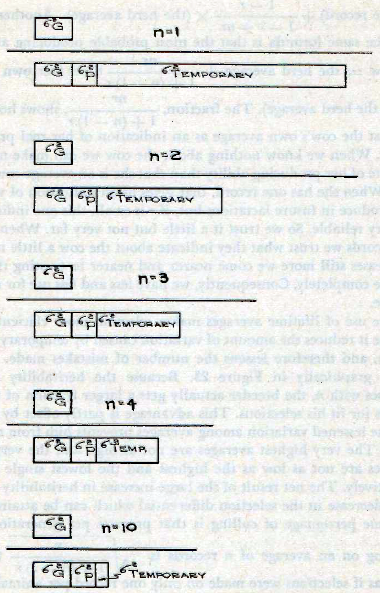
\includegraphics[width=\textwidth]{Figure_23.png}
    \caption{Diagram showing how the heritability of differences between averages
increases as the number ($n$) of records in each average increases. Drawn to scale for
the case in which heritability of differences is .12 when $n$ is 1 and repeatability of
single records is .20. That means the case in which 80 per cent of the variance
between animals with one record each is caused by temporary environmental circumstances.
$\sigma_G^2$ is the additively genetic variance between individuals. $\sigma_P^2$ is the variance
due to permanent but nontransmissible differences between individuals. These
include differences due to dominance deviations, epistatic deviations, and to such
effects of environment as are permanent for each animal but differ from one animal
to another. As $n$ increases, the variance due to temporary things falls to one $n$th of its
value in single records.}
    \label{fig:Lush_Figure_23}
\end{figure}

In records of yearly milk and fat production, considering only cows
which are in the same herd, $r$ is usually somewhere between \nicefrac{1}{3} and
\nicefrac{1}{2}. We shall not be far wrong if we take \nicefrac{2}{5} as the general figure to be
used in the preceding equation, although a higher figure would be justified
in herds where management has been unusually standardized and
corrections for the known environmental circumstances have been
unusually complete. In fact, $r$ is the fraction of the total variance among
the corrected records which is due to permanent differences between
cows; and $1 - r$ is the fraction of the variance caused by temporary circumstances
which vary from one record to another of the same cow.
\index{Variation!of averages|)}

\begin{table}[t]
	\centering
	\caption{\textsc{Progress When Selecting Between Animals With} $n$ 
	\textsc{Records Each, as a Multiple of the Progress Which Could Be Made by
	Selecting Between Them When They Had Only One Record Each}}
	\label{tbl:Lush_Table_13}
	\begin{tabular}{l|c|c|c|c|c|c|c|c|c}
		\hline
		\hline
		 		& \multicolumn{9}{c}{$r$} \\
		 \cline{2-10}
		 $n$	& .1	& .2	& .3	& .4	& .5	& .6	& .7	& .8	& .9 \\
		 \hline
		 2		& 1.35	& 1.29	& 1.24 	& 1.20 	& 1.15	& 1.12	& 1.08	& 1.05 	& 1.03 \\
		 3		& 1.58	& 1.46	& 1.37	& 1.29	& 1.22	& 1.17	& 1.12	& 1.07 	& 1.04 \\
		 4		& 1.75	& 1.58	& 1.45	& 1.35	& 1.26	& 1.20	& 1.14	& 1.08 	& 1.04 \\
		 6		& 2.00	& 1.73	& 1.55	& 1.41	& 1.31	& 1.22	& 1.15	& 1.10 	& 1.04 \\
		 10		& 2.29	& 1.89	& 1.64	& 1.47	& 1.35	& 1.25	& 1.17	& 1.10 	& 1.05 \\
		 \hline
	\end{tabular}
\end{table}

\noindent
More rigid control of the environment will naturally make $r$ higher.
That is, $r$ is a description of conditions in a particular population and
is not a fundamental biological constant. If we use the fraction \nicefrac{2}{5} in
the preceding example, the equation simplifies to: The cow's ability
\(= \dfrac{2n}{2n + 3} \times (\textrm{her own average}) + \dfrac{3}{2n + 3}
\times (\textrm{herd average})\).
That gives the following for estimates of the real producing ability of the three
cows: A = 480 pounds; B = 494 pounds; C = 516 pounds. C is probably
the best and A the poorest of these three, so far as the evidence
goes; but all three are good cows, and the differences between them are
small enough that we should not be greatly surprised if another lactation
or two would change their order.
\index{Environment and heredity|)}
\index{Regression|)}

Figure~\ref{fig:Lush_Figure_24} shows graphically the results of such computations for
butterfat production in an actual herd. The numbers along the vertical
scale are the barn numbers of the cows. Such a graphic scale of estimated
productive ability is a convenient help in making decisions about
culling the cows or saving bull calves from various cows. It must be
kept reasonably up to date, of course, if it is to be useful. At any particular
time some of the cows will have incomplete records which indicate
their producing ability but do not merit as much confidence as completed
records. In making Figure~\ref{fig:Lush_Figure_24}, the records estimated from lactations
still incompleted have arbitrarily been given about half as much
confidence as completed records in the case of cows which have not yet
completed their second record. The incomplete records were not used
at all for other cows. The heifers with only an incomplete lactation were
placed by themselves on the right to emphasize further the uncertainty
about their ability. The cows at the extreme left were included to show
whether those which left the herd either through death, disability, or
voluntary culling, had really averaged less in productive ability than
those which remained.

\begin{figure}[htbp]
	\centering
    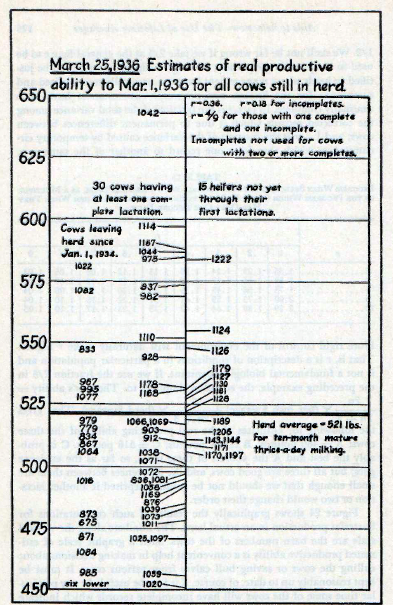
\includegraphics[width=\textwidth]{Figure_24.png}
    \caption{Estimated producing abilities of many cows with unequal numbers of
    		 lactations, based on all information available at the date when the
    		 scale was made.}
    \label{fig:Lush_Figure_24}
\end{figure}

Many other examples of the use of averages might be given. In each
of them it is necessary to know something about the repeatability of the
characteristic. In fertility of swine the repeatability of the number of
pigs born to the same sow in different litters is about one-sixth. In the
weight of fleeces shorn from sheep, the repeatability is about .5 to .6.
The corresponding figure for the fleece weights of Angora goats is about
.4. Some of the earliest studies on repeatability of production records in
farm animals were made on the records of first and second year egg production
in egg-laying contests. Most of those figures were of the order of
.45 to .60. All of these are computed on the basis of records made within
one herd or flock.

The method of averages can be extended to include scores\index{Scoring} or any
other ratings of type which can be expressed numerically. The repeatability
of such type ratings is usually low enough that there would be
a material gain in the accuracy of selections by obtaining and averaging
type ratings of the animal at different times in its life as compared with
relying upon the opinion of one judge, no matter how expert, who saw
the animal only once. The repeatability of type ratings of dairy cows at
intervals of one year was .34 to .55 in the only study\footnote{\textit{Jour.
of Dy. Sci.} 25:45--56, 1942} yet reported. The
opinions which the same judge would hold of the animal if he inspected
it at different times in its life usually vary more than do the opinions of
several judges who might inspect the animal at nearly the same time.
Probably this varies considerably with the class of animal and with the
ages at which the inspections are made.

The method of averaging repeated observations, of course, is limited
to characteristics which can be observed more than once. It cannot be
applied to such things as growth rates , age to sexual maturity, or to
carcass qualities which can be observed only upon slaughter of the
animals. It is also limited in usefulness for egg production, where such
a large part of the total economical lifetime production of the bird is
made during its first year.
\index{Repeatability|)}

Of course the costs of waiting to cull until more records are available
need to be considered, too. Besides the actual loss incurred by
keeping any animal which is not actually paying its way, such waiting
tends to make the interval between generations longer and thereby to
lower the progress \textit{per year}. This will partly offset the gain it makes by
increasing the progress \textit{per generation}. The costs of waiting to cull
would vary with the animal and with economic circumstances, being
higher with hens, for example, where the second year's production is
lower than the first, than with cows where the second record is generally
some 12 to 15 per cent higher than the first.

In the case of cows the first lactation will be several months along
and the heifer may be with calf again before it is certain that the production
in her first lactation will be very low. Often it will not cost
much then to keep her enough longer for the first three or four months
of the second lactation to confirm or disprove what the first lactation
indicated. A practical rule for many herds is to cull in their first lactations
only those with extremely low production, keeping the moderately
low and doubtful ones through the flush of production in their second
lactations. They will usually pay at least their feed costs for that,
since so much of the production comes in the first half of the lactation.

In many cases the decision to keep or cull must be made while the
animals are young if economic loss is to be avoided. For example, with
range cattle or sheep the heifer calves and ewe lambs can usually be
sold to better advantage and with lower feed costs at or soon after weaning
age than if they are kept much longer. The ranchman could cull
them more accurately if he could wait until they grow up and until he
can have rated their type several times, but the gain from doing this
may not be enough to pay for the loss he will take in lower sale prices
for those which are finally culled after they are too old to be sold as
heifer calves or lambs.

\index{Abnormal records|(}One practical problem involved in using lifetime averages is what
to do with records thought to have been made under abnormal conditions
for which no satisfactory correction is known. In principle such
records should be omitted. The practical difficulty is how to decide
fairly when conditions really were abnormal.\index{Abnormal records|)} Some circumstances are
definite enough that they offer no difficulty. For example, in Denmark
records are omitted for years in which the cow aborted or had foot-and-mouth
disease. No other omissions are permitted. Other circumstances
are not definite enough to permit a clear decision. For example, a cow
may have had a bad attack of milk fever at the beginning of her lactation.
The owner may believe that she did not recover soon enough to
produce normally during that lactation. But how is one to be certain?
To base the decision on the size of the record opens the door to all
kinds of biases. The guiding principle should be to omit no record
except when the circumstances are so definite that no doubt can exist.
Those circumstances must be something other than the size of the record
of performance itself.

Basing selections on lifetime averages will automatically foster some
selection for longevity and real ``constitution,'' since breeders will tend
to save for sires only the sons of females which have proved themselves
by several records of production. When selections are based on lifetime
averages, it will hardly be possible for a heifer or gilt with only one
record of production to get her son saved to head a purebred herd
unless that one record was truly phenomenal.

\section*{SUMMARY}

The use of an average of many repeated observations as a basis of
selection is one of the most effective ways of overcoming mistakes and
confusion which would otherwise result from the effects of temporary
environmental conditions. The method is inexpensive, requiring only
the existence of the records, the time needed for averaging them, and
whatever it costs to postpone culling until two or more observations
have been made. It can be made to foster some selection for longevity
and constitution. In using such lifetime averages, allowance must be
made for the lessened variability of averages which are based on many
records. If this is not done, it will appear that most of the extreme producers,
both high and low, are individuals with only one or at most
two records. The method is needed most for things which are least constant
from one time to another in the animal's life. Much of the gain
from using it comes with the second record, but if $r$ is small the gain
from waiting for a third or even a fourth record may be considerable.
The method does not help at all to keep the breeder from being
deceived by permanent effects of environment, such as permanent
stunting when young, nor by the consequences of dominance and complex
gene interactions. Placing much reliance on selecting animals by
their lifetime averages will naturally lead men generally to buy breeding
stock from herds which they know well and in which they have
had several opportunities to study the animals.
\index{Lifetime Averages|)}
\chapter{Aids to Selection --- Pedigree Estimates}
\label{cha:Lush_Chapter_14}
\index{Pedigrees as aids to selection|(}

\begin{quote}
``The bull gives no milk, of course, yet will not a bull descended from several generations
of high-producing dams produce, when mated with a highly productive cow,
calves which possess this characteristic to a still higher degree?'' --- Bergen, in 1780.
\end{quote}

The decision of whether to reject or keep an animal for breeding
may be modified by what its relatives are or do. Wherever that is done,
the intensity of individual selection is reduced. The average individual
merit of those selected must be lowered every time an animal which
would be rejected on account of its own individuality is kept for breeding
because it has unusually excellent relatives, or every time an individually
excellent animal is rejected because its relatives are of low
merit.

By paying a reasonable amount of attention to the relatives it may
be possible to increase the genetic accuracy of the selections more than
enough to offset the decrease in the intensity of selection for individual
merit. There is real danger of doing damage by paying too much attention
to the relatives, since they are not a perfect guide to the individual's
breeding value either. The proper balance between paying too
much and paying too little attention to the merits of the relatives shifts
from case to case according to how well the merits of the relatives are
known, how closely they are related to this animal, how well the individual
merit of this animal is known, and how highly hereditary the
characteristics are. An understanding of the principles and practical
difficulties involved will help in using the approximate rules which in
actual practice must guide us in estimating an individual's breeding
value from what we know about the merit of its relatives.

From the genetic principles involved, relatives of an individual may
all be grouped in two classes: those which are related to it through its
parents and those which are its descendants. The former group is considered
here collectively under the general term of ``pedigree,'' which is
the subject of this chapter, while the latter group will be considered in
the next chapter under the term of ``progeny test.''\index{Progeny test}

Attention to pedigree can make selection more effective only
because individual selections are not perfectly accurate. We never know
exactly what genes an individual has. Our knowledge of that is especially
scanty when the animal is still immature, as many are when first
selections must be made. If we estimate its inheritance from its own
appearance or performance, we will make some mistakes on account of
the effects of environment, dominance, and complex interactions of
genes. If we estimate its inheritance by paying attention to the individuality
and performance of its relatives, we may avoid some of those
mistakes; but we run the risk of introducing other mistakes, because
those relatives will not have exactly the same genes as this animal does.
Moreover, our estimate of the genes in those relatives is itself subject to
error from our being confused by the effects of dominance, environment,
and complex gene interactions on those relatives.

\section*{GENERAL PRINCIPLES WHICH LIMIT THE USEFULNESS OF PEDIGREES}
\index{Sampling nature of inheritance|(}

The biological basis for the usefulness of pedigrees lies in the fact
that an individual gets half of its inheritance from its sire and half from
its dam. If we knew what inheritance these parents had, we could estimate
what inheritance this individual probably received from them.
Because the parents were heterozygous for some of their genes, such
estimates cannot be perfectly accurate. Chance at Mendelian segregation
plays a part in determining what the parents transmit to any one
offspring. An additional limitation on the use of pedigrees is that we
will rarely know exactly what genes the parents did have, although we
will often know more about their inheritance than about the inheritance
of each of the offspring, because the parents have had a longer
time in which to demonstrate their characteristics or performance. Also,
because some of the ancestors will have had other offspring, they will be
to some extent progeny-tested, whereas most individual selections must
be made before any progeny are available.

Even if we knew exactly what genes each parent had --- and no
amount of pedigree study could tell us that much --- the sampling nature
of inheritance limits the average likeness between the inheritance of an
individual and the inheritance of either parent in a random breeding
population to a correlation of $+$ .50. On the same basis the correlation
between an individual and the average of its two parents is $+$ .71. If
much inbreeding, or mating of like to like where ideals are diverse, is
being practiced, these correlations will be larger; but in any actual
population they will be far from perfect. If we are trying to predict the
average merit of many offspring, the effects of chance at segregation will
tend to cancel each other. The correlation between the inheritance of
one parent and the average kind of inheritance of $n$ of its offspring
approaches $+$ 1.00 according to the formula \(\sqrt{\dfrac{n}{n + 3}}\)
if the other parents of those offspring are a random sample of the breed. The correlation
between the average inheritance of both parents and the average
inheritance of $n$ of their offspring approaches $+$ 1.00 according to the
formula \(\sqrt{\dfrac{n}{n + 1}}\).\footnote{\textit{See also} page 260.}
These correlations are between genotypes and not between the directly
observable characteristics of the animals, but the formulas explain what
seems at first to be a contradiction between the facts that pedigrees cannot
be highly accurate for estimating what an individual animal will be and yet
can be very accurate in predicting the average qualities of a large number
of offspring from one pair of parents.
\index{Sampling nature of inheritance|)}

\index{Ancestors, importance of various ones|(}
If we knew exactly what genes the sire and dam each had, nothing
would be gained by considering more distant ancestors or collateral
relatives. Figure~\ref{fig:Lush_Figure_25} shows a Mendelian example
of that with respect to one pair of genes.

\begin{figure}
	\centering
    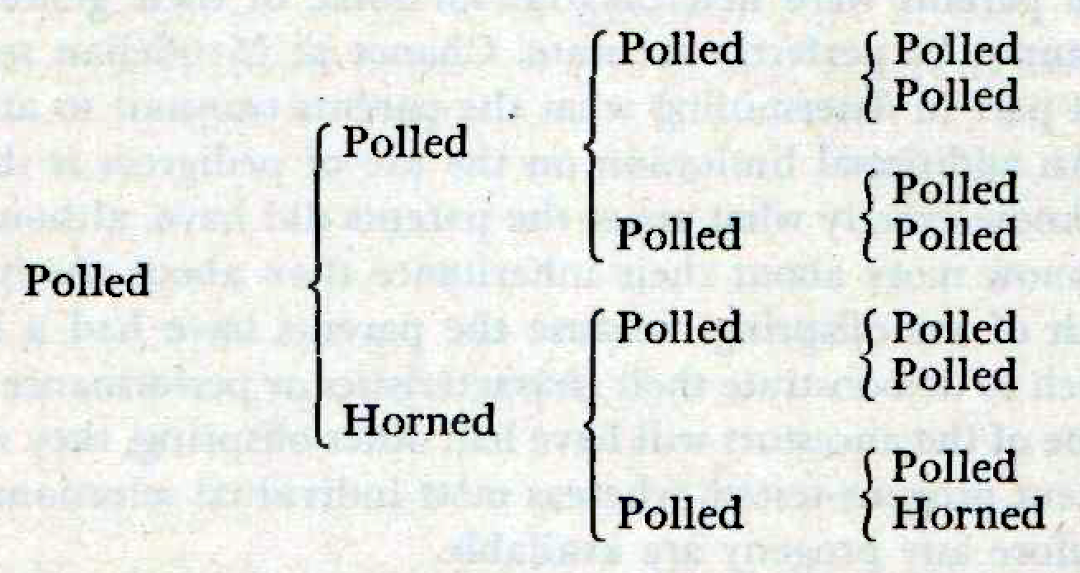
\includegraphics[width=\textwidth]{Figure_25.png}
    \caption{A pedigree of a Polled Hereford, illustrating the general principle that
			 study of remote ancestors tells nothing more about an animal's inheritance when the
			 genotype of an intervening ancestor is known with certainty.}
    \label{fig:Lush_Figure_25}
\end{figure}

Insofar as we are correct in thinking that horned cattle are \textit{pp} and
polled cattle are either \textit{PP} or \textit{Pp}, it is certain that the dam
in Figure~\ref{fig:Lush_Figure_25}
was \textit{pp} and that this offspring of hers is \textit{Pp}. No amount of study of her
ancestors would add anything to our knowledge of that. That brings us
to the question of how much attention to pay to each ancestor in the
general case where we know something about the individual merit of
most ancestors but are not entirely sure of the genotype of any of them.
The answer to that question depends on five different circumstances:
First, how closely the ancestor is related to the subject of the pedigree;
second, how completely the merit of each ancestor is known; third, how
well the merit of intervening ancestors is known; fourth, how highly
hereditary the characteristic is; fifth, how much environmental correlation
there is between ancestor and subject and between different
ancestors.

The general fact that an animal gets half of its inheritance from
each parent would naturally lead to one form of what is generally called\index{Galton's ``Law''}
``Galton's law'' --- of which more is said in chapter 20 --- namely: In estimating
an individual from knowledge about one of its parents, it
should be estimated as equal to one-half of that parent plus one-half of
the breed average; if it is being estimated from a grandparent, it should
be estimated at one-fourth of that grandparent plus three-fourths of the
breed average; with a great grandparent, it should be one-eighth of that
great grandparent plus seven-eighths of the breed average, etc. The
importance of the ancestor in such a prediction equation is halved with
each additional generation which intervenes between the individual
and its ancestor. This ``law'' in general is sound in a random breeding
population, provided only one ancestor is being considered and provided
some conservatism is practiced by basing a smaller share of the
estimate on the ancestor and a correspondingly larger share on the
breed average wherever the characteristic is not highly hereditary or
there is uncertainty that the information about the ancestor really is a
true picture of its inheritance. Two ancestors cannot both be used in a
single prediction of this kind if one of them is an ancestor of the other.
We could combine information about the sire and the maternal grandsire,
estimating the animal at one-half of the sire plus one-fourth of the
maternal grandsire plus one-fourth of the breed average, with still more
emphasis on the breed average as we are less sure that what we know
about the sire and grandsire is really typical of their breeding value.
But we could not combine information about the sire and the paternal
grandsire in the same way because, to a considerable extent, the things
which could be estimated from knowledge of the grandsire are the same
things which could be estimated better from knowledge of the sire himself.
The use of both in a single prediction would be using some of the
information a second time.

Czekanowski\footnote{Zeit. f. Ind. Abst. u. Vererbungslehre 64:154--68. 1933.}
has explored the question of the comparative importance
of sire, grandsire, and great grandsire in the special case when (1)
all three are in the same line of descent, (2) no other ancestors are considered
(3) exposure of relatives to the same kind of environment has
contributed nothing to the correlation between them, and (4) the merits
of all three ancestors are equally well known. His figures for the
amount of attention (the net regression coefficient) to be given each of
these three ancestors for several values of the correlation between parent
and offspring are as follows:

\begin{table}[htbp]
	\centering
	\begin{tabular}{l|c|c|c|c|c|c|c}
		\hline
		\hline
		 				& \multicolumn{7}{c}{Correlation Between Parent and Offspring} \\
		 				\cline{2-8}
		 				& .10 &	.20 &	.25	& .33	& .40	& .44	& .50 \\
		\hline
		Sire			& .095	& .186	& .232	& .312	& .381	& .431	& .500 \\
		Grandsire		& .039	& .059	& .062	& .059	& .046	& .030	& .000 \\
		Great grandsire	& .016	& .020	& .018	& .012	& .006	& .002	& .000 \\
		\hline
	\end{tabular}
\end{table}

\noindent
The figures show how little is to be gained by considering the remote
ancestors when the merit of the intervening ones is equally well known.
For highly hereditary characteristics the sire's own appearance or performance
is almost a perfect guide to the net worth of his inheritance.
For slightly hereditary characteristics, relatively more attention should
be paid to the remote ancestors, but in that case the predictive value of
pedigree is low anyhow, no matter how used. It is doubtful whether
Czekanowski's figures have any practical usefulness beyond demonstrating
these genera l principles. In actual practice some ancestors will
be much better known than others. For example, if the sire in Czekanowski's
problem were still too young for his mature characteristics to
be unmistakable or if the grandsire were thoroughly progeny-tested\index{Progeny test},
less attention should be given to the sire and more to the grandsire than
these figures indicate.

\index{Collateral relatives}
Collateral relatives in the pedigree are a progeny test which furnishes
evidence about the genotypes of their parents or grandparents.
Although a grandparent is generally as good an indicator of an individual's
inheritance as a half brother or sister, an individual can have
only four grandparents but may have a much larger number of half
brothers and sisters. In case it does, an estimate of its inheritance based
on the appearance and performance of its half brothers and sisters may
be much more accurate than an estimate based on its grandparents. The
evidence furnished by collateral relatives should be used in the pedigree
according to what it shows about the kind of inheritance which
the mutual ancestor had and according to the completeness of the evidence.
For example, in a dairy pedigree where the production of a
large number of paternal half sisters is known, the sire may be considered
reasonably well proved, and there is little to be gained by studying
his ancestors. If the dam in the same pedigree is still a young cow in her
first lactation, considerable information could be gained by considering
the maternal grandparents, although consideration of the paternal
grandparents would be of little use.
\index{Ancestors, importance of various ones|)}

The chief danger in pedigree selection is that it will do more harm
by lowering the intensity of individual selection than it does good by
making the selection more accurate. Pedigree is not often as accurate a
basis for estimating breeding value as individuality is,\footnote{In a random
breeding population in the limiting case most favorable to confidence
in the pedigree --- the case where the genotypes of sire and dam are perfectly
known --- the correlation between an animal's breeding value and its own individual
appearance or performance is \(\sqrt{2a}\) times as large as the correlation between its breeding
value and the average genotype of its parents, where $a$ is the additive genetic
fraction of the variance in individual appearance or performance. This relation indicates
the basis for the general principle that pedigree can become more dependable
than individuality for characteristics which are slightly hereditary (i.e., where $a$ is
less than \nicefrac{1}{2}), provided the parents are so thoroughly known that there is little
doubt about their genotypes.} although it will
occasionally be so in a hitherto unselected population, especially if the
individuals being selected are still too young to have had much chance
to prove their characteristics at the time the selection must be made.
Pedigree selection is rarely as useful in animal breeding as it can be at
times in plant breeding, because there is almost nothing in animal
breeding to correspond to the distinct and uniform lines or families
which exist in those plant species, such as wheat and cotton, where self-fertilization
or some other intensive form of inbreeding is the rule. In
plants in which self-fertilization is possible, an individual may have
only one parent, only one grandparent, one great grandparent, etc., and
each of these may be more thoroughly progeny-tested than is possible
where reproduction must be bi-parental.

\section*{PRACTICAL LIMITATIONS ON THE USEFULNESS OF COMMERCIAL PEDIGREES}

Often pedigrees contain little information except the names and
numbers of the ancestors. To use them at all, you must find from other
sources how excellent or poor those ancestors were. That is less true of
dairy and poultry pedigrees than of others and is being improved in the
pedigrees of most kinds of livestock; but, as printed today, many pedigrees
are only a meaningless genealogical jumble of names and numbers
to one who does not know from other sources how meritorious
those ancestors were. This limitation does not matter much to the man
who is thoroughly familiar with his breed. Perhaps all purebred breeders
should aim at that goal, but an enormous number of potential customers
and even many breeders simply have not time nor opportunity
to keep familiar with the merits and deficiencies of the prominent
breeding animals of their breed. Pedigrees would be more useful to
these men if more information were included about the merits of the
ancestors, even if that meant only printing the pedigree as far the
parents and grandparents. In justice to those who print the pedigrees,
it should be emphasized that in most cases there is no information to
print because no systematic plan of measuring and recording the merit
of individual animals has ever been in operation.

This is no new idea. As long ago as 1832 the following was written
in \textit{The Thoroughbred Horse in Prussia}: ``If they do not contain production
tests, such herdbooks will be useless and without interest, since
they would contain only names of which no one knows anything and
which mean nothing.''

Such information as is given in the pedigrees is usually selected to
show the animal in the most favorable light possible. Actual falsehoods
in printed pedigrees are rare because of the heavy penalties in loss of
business which are exacted of a breeder who is suspected of dishonesty;
but plenty of \index{``Filler'' in pedigrees|(}``filler'' is still used,
although general practice in this
respect is improving. An example of ``filler'' is shown in Figure~\ref{fig:Lush_Figure_26}. The
information printed under an ancestor's name applies in many cases to
half sisters of its parents or grandparents or even to more remote relatives.
The following statement was found listed under the paternal
grandsire in a pedigree of a bull used in a large dairy herd in Iowa in
1937. ``His dam is a granddaughter of that noted transmitter, Sir
$\cdots\cdots$, sire of $\cdots\cdots$'' The actual records
mentioned here were made by cows separated by six Mendelian segregations
from the bull in whose pedigree they appeared, and related to
him less than 2 per cent. By contrast Figure~\ref{fig:Lush_Figure_27} shows a pedigree in
which each bit of information is listed under the ancestor which it most
directly concerns.
\nowidow

Generally the ancestors were selected individuals from among their
contemporaries. That is especially likely to have been true of the males
and hence of their ancestors. Some regression to the breed average is to
be expected for that reason, even if the pedigree information is supplied
by an utterly impartial and accurate agency. The intensity of the
selection practiced in choosing those ancestors is not usually known.

In most pedigrees little information is given about collateral relatives.
That is beginning to be remedied in dairy cattle and poultry
pedigrees by the inclusion of progeny tests wherever those are available.
Occasionally in the pedigrees of meat animals one finds comments
on the winnings or performance of brothers or other collateral relatives.
Information about \index{Collateral relatives}collateral relatives may be much more highly
selected than information concerning ancestors, since there can be no
choosing of ancestors to be mentioned but only selection of data
concerning them; whereas among the \index{Collateral relatives}collateral relatives there may be
choice of which individuals shall be mentioned and also selection of
the best records of those individuals. One often finds in dairy pedigrees
such comments as ``20 A.R. daughters, two with over 1,000 pounds of
fat.'' Since the records of 18 of the 20 are omitted and the number of
daughters not tested is not stated, such a statement tells little more than
that this sire was used extensively and was regarded highly enough that
20 of his daughters were tested officially.

\begin{figure}
	\centering
    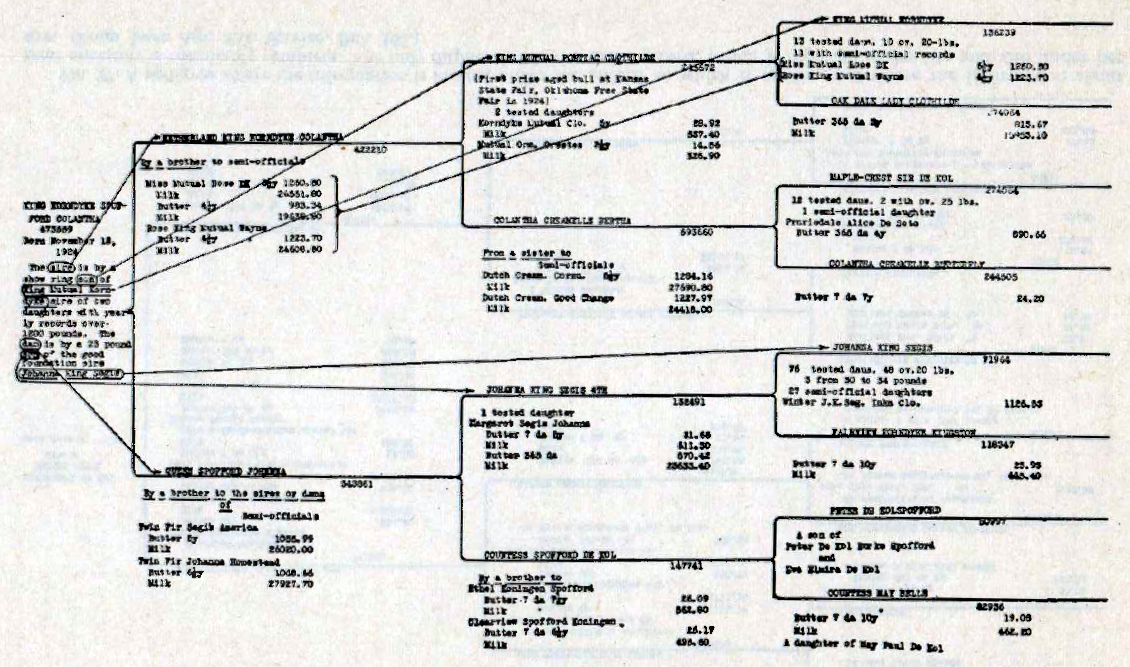
\includegraphics[width=\textwidth]{Figure_26.png}
    \caption{A pedigree showing a moderate amount of ``filler.'' Favorable
    		 items are repeated several times and are placed under animals
    		 rather distantly related to those on whose inheritance the
    		 items throw most light. (From Iowa Agr. Ext. Service, Bul. 162.)}
    \label{fig:Lush_Figure_26}
\end{figure}

\index{``Filler'' in pedigrees|)}

\begin{figure}
	\centering
    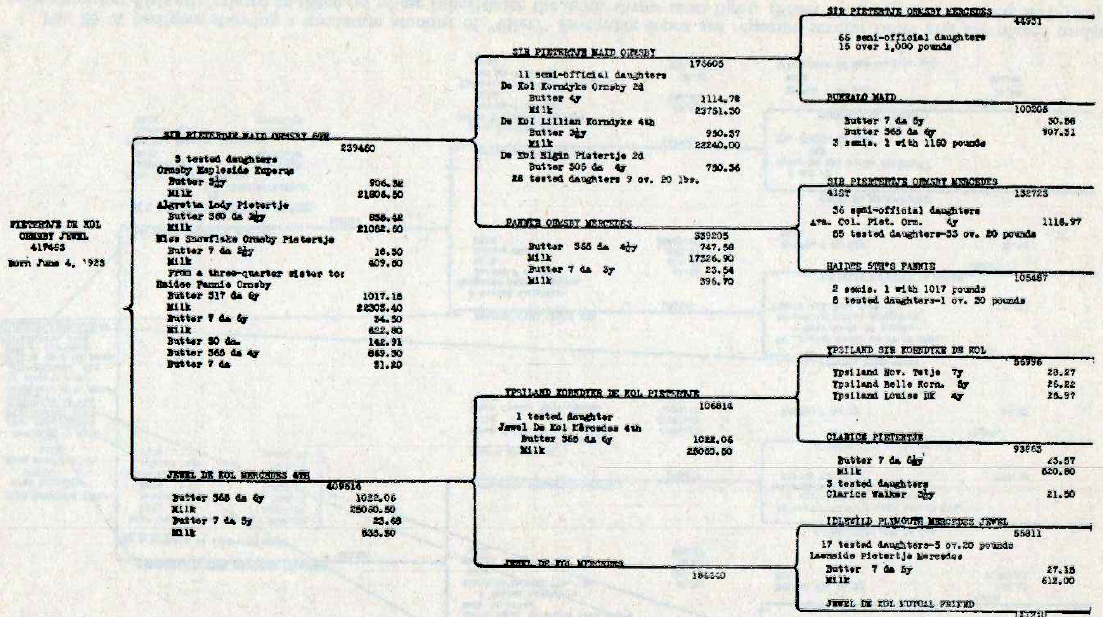
\includegraphics[width=\textwidth]{Figure_27.png}
    \caption{A pedigree showing a moderate amount of ``filler.'' Favorable
    		 items are repeated several times and are placed under animals
    		 rather distantly related to those on whose inheritance the
    		 items throw most light. (From Iowa Agr. Ext. Service, Bul. 162.)}
    \label{fig:Lush_Figure_27}
\end{figure}

Usually no average pedigree of the breed is available for comparison
with the one being considered. That lack would not bother the man
who has studied enough pedigrees of his chosen breed to get a fairly
definite idea of what a typical pedigree is, but many people simply cannot
spare the time for such study or <lo not have access to enough pedigrees
to learn what is typical for the breed.
\noclub

In a sense individual select ion is pedigree selection for the next
generation. When the parents have been selected for individuality, the
offspring which would have had the worst pedigrees are not permitted
to be born! Much of the use which might be made of pedigree selection
in a hitherto unselected population is simply not available to the breeder
who is pursuing the same goal which was pursued by those who bred
and selected the parents of his animals. This sets further limits to the
usefulness of pedigree selection under ordinary practical circumstances.
There are some exceptions to this general situation. One is the fact that
fewer males than females are needed for breeding. After the males are
born there can be much pedigree selection among them, although there
cannot be much among females. This is what a cattle breeder does when
he decides he will save a calf from a certain cow if it is a heifer but not if
it is a bull. When a breeder's ideals differ distinctly from those of many
of his fellows and he lays much importance on things which they consider
unimportant and vice versa, the pedigrees of their animals offer
him considerable opportunity for selection if he purchases from them.
Also, when the ideal of a breed changes, there is momentarily a reappraisal
of the merits of the ancestors. While that is happening there is
opportunity for pedigree selection on the new basis for a generation or
two. Selection among the parents does not reduce the variability among
their offspring nearly as much as it does the variability among the parents
themselves. Hence in a population which has already been under
selection for a generation or two there is much more opportunity for
selecting the offspring on their individuality than on their pedigrees.

\section*{ERRORS WHICH MAY BE CORRECTED BY PEDIGREE SELECTION}

Pedigree selection helps to overcome deception by environment
because it does not often happen that the ancestors were all kept under
the same environment.

Pedigree study would be of some help in overcoming deception by
\index{Dominance}dominance if full information about the collateral
relatives were presented,
but that is rarely done. If the recessive is rare and only the direct
ancestors are given, pedigree is almost no help in this respect. For example,
pedigrees do not help in eliminating red in the black breeds of
cattle, since all ancestors are black and the existence of red sibs or aunts
or uncles or other collateral relatives is not mentioned. The parents of
red calves and something more than half of the sibs of red calves are
heterozygotes. Culling them because of their relationship to the red animal
would make the genes for red scarcer than can be done by culling
the red alone, but present pedigrees do not give the information which
would permit that. Nor is it likely that breeders would report such
information if it were to be used to reflect unfavorably upon animals
they have for sale. Pedigrees help a little in overcoming deceptions by
dominance in such cases as the polled Herefords where the distinction
between horned and polled is shown in the pedigree.\footnote{The
probability that a polled calf from polled parents is homozygous for the
gene for polledness is equal to \(\dfrac{1 + s + d + sd}{3 + s + d - sd}\)
where $s$ is the probability that the sire is \index{Homozygosis}homozygous and $d$ is the
probability that the dam is homozygous. Probability is expressed on a scale
ranging from zero for absolute impossibility to 1.0 for absolute
certainty.}

Pedigree studies may help considerably in overcoming the deceiving
effects of \index{Epistatic effects}complex gene interaction. An unusually good animal from
poor or mediocre stock on both sides always suggests that this animal is
the result of a lucky combination of several genes all of which are necessary
in order to permit each to manifest its desirable effects. The occurrence
of such an animal is often called ``nicking.'' In that case the
animal would almost certainly be heterozygous for many of the genes
whose cooperation is required. There would be small chance of its
transmitting enough of those genes in each gamete to cause this excellence
to reappear in many of its offspring. Likewise, a poor individual
with excellent ancestors and relatives on both sides will be suspected of
lacking just a few genes which are necessary for the successful operation
of the other genes for the excellent qualities of his family. It will be suspected
that he has many good genes which do not manifest their presence
in him. If he were used for breeding, many of his mates would
transmit to their offspring the necessary genes he lacks. He may be preferred
to a better individual from a poorer family, although, of course,
he would be discarded if there were enough good individuals in his own
family.

\section*{RULES FOB THE USE OF PEDIGREES IN SELECTION}

In evaluating a pedigree one should estimate what kind of inheritance
the sire and the dam had and then average those two estimates.
Wherever there is uncertainty about an individual's inheritance, conservatism
requires that it should be estimated closer to the average of
its breed or herd than the evidence about it, if accepted at face value,
indicates it to be. Thus, if there is much evidence about the sire but
only a little about the dam, the estimate should give much weight to the
sire but most of the weight which would have gone to the dam should
be placed on the breed or herd average\index{Regression}. The estimate of the sire's inheritance,
or of the dam's inheritance, is made similarly by averaging the
inheritance of its sire or dam and then modifying that average by what
its own individual merit seems to be, using the general principle that
the individual's own merit should receive more weight than its pedigree
under most circumstances. For characteristics which are but slightly
hereditary or in cases where the ancestors' merits are much better
known than the individual's merit --- as, for example, where the ancestors
are well progeny-tested or have long lifetime records while the individual
is still immature --- it may be correct to attach more weight to
pedigree than to individual merit.

The more certainly an ancestor's merit is known, the less weight
should be placed on its ancestors. This is difficult to place on a quantitative
basis, but Czekanowski's table will give a rough idea of about
what that relation should be when two ancestors in the same line are
equally well known. If the breeding value of the nearer ancestor is
known with much more certainty than that of the more remote ancestor,
there is scarcely any use to pay attention to the more remote
ancestor.

If there is reason to think that much sex-linkage\index{Sex linkage} is involved in a
particular case, the proper procedure is to give the sire more weight in
estimating the inheritance of female offspring and to give the dam more
weight in estimating the inheritance of male offspring. (See page \pageref{page255}
for reasons.) The principle of conservatism in cases where the merit of
the two parents is not equally known can also give rise to unequal
weighting. Thus, in dairy pedigrees where the sire is too young to be
progeny-tested but the dam's production is known, much weight can be
placed on the dam, but only a little on the sire on account of the uncertainty
about the sire's side of the pedigree. In another dairy pedigree
where the sire is well progeny-tested but the dam is a young heifer in
her first lactation, the situation may be reversed, with more weight
being put on the sire's side of the pedigree, only a little on the dam,
some on her pedigree, and much on the breed average for conservatism
in her case.
\noclub[3]

Because the ancestors are in most cases selected animals and
because the information about them is selected to show them in a favorable
light, allowance should be made for regression toward the breed
average. There seems to be no quantitative rule for doing that except
the general one that the more extreme the selection is believed to have
been among the parents or in the information presented concerning
them, the more allowance should be made for regression.
\nowidow

\section*{SUMMARY}

The accuracy of pedigree selection is limited because of the sampling
nature of inheritance wherever genes are heterozygous. This
makes it impossible to be exactly sure of what an individual offspring
will be, even if one were in the extreme position of knowing exactly
what inheritance its sire and dam had.

The accuracy of pedigree selection is further limited in practice
because one is never entirely sure of the inheritance the parents had,
since that, too, must be estimated from their own appearance or performance
or from that of various of their relatives.

A limited amount of attention to pedigree will make the selections
more accurate, but it necessarily cuts down on the intensity of the individual
selection which can be practiced. Too much attention to pedigree
may do more harm by decreasing the intensity of individual
selection than it will do good by increasing accuracy, since pedigree
selection is not perfectly accurate either.

The use of pedigrees is based on the principles: that inheritance is
approximately equal from sire and from dam, and that, wherever one's
knowledge of the inheritance of the relatives is uncertain, one should be
conservative and estimate that the individual is somewhat nearer to the
breed average than the performance of its relatives.

Rarely should the pedigree receive as much weight as the animal's
own appearance or performance, although that can happen for slightly
hereditary characteristics if the merit of parents and grandparents is
much better known than the individual's own merit, either because
those ancestors are well progeny-tested or because the individual is still
too young to show its merits as unmistakably as its parents and grandparents
do.

Collateral relatives constitute progeny tests of some ancestor. They
therefore make the estimate of its inheritance more certain. If an animal
is well progeny-tested, little will be gained by studying the ancestors
back of it in the pedigree.

The proper amount of attention to pay to different relatives
depends on the closeness of their relationship to the subject of the pedigree,
upon how many of them there are, upon how completely the merit
of each other relative is known, and upon how highly hereditary the
characteristic is.
\nowidow

Because the ancestors are usually selected individuals, some regression
toward the breed average is to be expected . Moreover, the information
about the ancestors is usually selected to make them appear in the
most favorable light. For that reason more regression is to be expected.
Serious defects in the practical use of pedigrees include the fact that
the merit of collateral relatives such as sibs, uncles, cousins, etc ., is rarely
mentioned. If it is mentioned, it usually concerns only certain individuals
selected to make the pedigree more attractive and, moreover, is
selected information about those.

In most commercial pedigrees, other than those for dairy cattle and
poultry, little information of any kind is included except the names
and identifying numbers of the animal. Such a pedigree is useful only
to the extent that one knows or can find from some other source how
meritorious or mediocre those ancestors were.

In a breed which has been selected steadily toward the same goal for
two or more generations, there often is only a little room to practice
pedigree selection because the worst individuals among those which
might have become ancestors were eliminated by individual selection.
Therefore, the individuals which might have had the worst pedigrees, if
there had been no selection, simply do not get born.

The general conclusion regarding pedigree selection is that it should
usually be a minor accessory to individual selection, being permitted to
sway the balance in making decisions which are fairly close on individual
merit. It is most needed for characteristics which are not very
hereditary, for characteristics which only one sex can manifest, and
in selections which must be made while the animals are yet too young
to show clearly in their own appearance or performance what their
individual merit is.

The kind of errors in individual selection which are most likely to
be remedied by pedigree selection are those arising from the immaturity
of the individual and from mistaking differences caused by environment
and epistatic interactions for differences in breeding value. It
helps remedy errors caused by dominance when fairly full information
about collateral relatives is included, but is not of much help in this
respect when only the ancestors are described.

\section*{REFERENCES}

\begin{hangparas}{0.5in}{1}%
Marshall, F. R. 1911. Breeding farm animals. pp. 93--101.

Wriedt, Christian. 1930. Heredity in livestock. (Especially the chapter on ``Valuation
of Pedigree,'' pp . 168--72. Also pp. 6--10.) New York: The Macmillan
Company.
\end{hangparas}
\index{Pedigrees as aids to selection|)}
`\chapter{Aids to Selection --- Progeny Tests}
\label{cha:Lush_Chapter_15}
\index{Progeny test|(}

\begin{quote}
``The quality of a ram can usually be determined from his conformation
and from his get.'' ``You may judge them by their get if
their lambs are of good quality.'' --- Varro. The Husbandry of Livestock,
the first century \textsc{B.C.}
\end{quote}

\begin{quote}
``One may consider the ancestors as thoroughbred only when
all the progeny are thoroughbred.'' --- Thaer, in 1806
\end{quote}

By progeny test is meant estimating the individual's heredity by
studying its offspring. The general idea is an old one, as is indicated by
Varro's comments some 2,000 years ago. As long ago as 1826 Andre
recommended progeny testing as one of the main purposes for keeping
herdbooks for sheep. On page 299 in the USDA Yearbook for 1894,
the proving of bulls and the continued use of sires of proved excellence
are urged.

The principles of the progeny test come from the sampling nature of
inheritance. Each offspring receives from the parent a sample half of
that parent's inheritance. Each additional offspring receives another
independent sample from the same source. If one can find out what was
in several such samples, he will be fairly sure of what was in the parent.
A crude analogy may make the case clearer. If a barrel contained 100
apples, of which a certain number were ripe while the rest were green,
and if we could not get in the barrel to count the apples but could
count a sample half of them taken at random, we could tell within certain
limits what proportion of the apples in the barrel were ripe. There
would be a high degree of uncertainty about our estimate because this
one sample might by chance have contained considerably more or less
than a fair share of the ripe apples. If the sample half could be placed
back in the barrel and thoroughly mixed with the others and then a
fresh sample half could be counted and if that process were repeated
often enough, we could finally come to the point of knowing how many
apples were ripe and how many were green in the whole barrel,
although it would take several such samples for us to be sure that we
were within three or four of the right number.

The first practical difficulty encountered in using the progeny test is
that we do not know exactly what genes the offspring have. We can be
deceived by the effects of environment, dominance, and complex interactions
of genes in the offspring, just as we could in estimating the parent's
genes from its own appearance or performance. There is this important
difference, however: There are several of the offspring and the
deceiving effects of environment, dominance, and epistasis have an
opportunity to cancel each other. Thus, there is a chance for us to know
the average inheritance of the offspring with more certainty than we
know the inheritance of the parent. The parent is only one individual
and in it there has been no chance for the plus and minus errors to have
been canceled by averaging.

The second practical difficulty encountered in using the progeny
test is that each offspring also has received half of its inheritance from
its other parent. Since we usually do not know exactly what was in that
parent and will be still farther from knowing just what it contributed
to this particular offspring, we are often in doubt as to whether a certain
good quality in one offspring came from its sire or from its dam.
One way of overcoming this difficulty partially is to use all the available
information to estimate the other parent's inheritance; then allow for
that according to the general rule that the phenotype of an unselected
offspring will tend to average half way between the genetic values of its
two parents. Let \textit{X} represent the unknown genetic value of the parent
being progeny-tested and \textit{Y} be our estimate of the genetic value of the
other parent of an offspring which has a phenotype, \textit{P}.\index{Sire indexes} Then the most
probable value of \textit{P} is \(\dfrac{X + Y}{2}\) and the equation,
\(X = 2P - Y\) furnishes an estimate of \textit{X}, although not a very dependable one when
there is only one offspring, since Mendelian sampling variations, environmental
effects, etc., can have made \textit{P} in a particular case deviate
widely from the general rule. Also, of course, we may be rather wide of
the mark in our estimate of \textit{Y}. Another way of overcoming this difficulty
consists of progeny-testing an animal by breeding it to a large number
of different mates, in the hope that the merits and defects of those other
parents would just about cancel each other. Any general difference,
then, between the average of the progeny and the average of the breed
could be credited to the common parent. This method might, of course,
lead to large errors if the other parents were so selected that their average
merit was distinctly different from the breed average.

Theoretically, a third way of not being confused by what the other
parent transmitted is to use a special ``tester strain''\index{Lethal genes}\index{Tester strains|(} so constituted
genetically that their contribution to the inheritance of the offspring
will not hide the inheritance received from the parent being progeny-tested.
Occasionally this can be done in actual practice. Examples are
the use of red cows to test the \index{Homozygosis}homozygosis of bulls belonging to black
breeds, or the use of horned cows to test the homozygosis of polled
bulls.\footnote{If a black bull is mated to red cows and produces even one
red calf, he is known to be heterozygous. If he produces only black calves,
he is probably homozygous, the assurance of that increasing with the number
of calves thus produced. The laws of chance governing the case are such that
if a heterozygous black bull sires one calf from a red cow, that calf is just
as likely as not to be black; but, if he sires two calves, there is only 1
chance in 4 that both will be black; there is 1 chance in 8 that three
such calves will all be black, 1 chance in 16 with four calves, 1 chance in 32 with five
calves, etc., the chance being \(\left(\dfrac{1}{2}\right)^n\) where $n$ is the number of calves sired. Hence, if
a black bull has sired more than five or six calves from red cows and none of th~
calves are red, the chance that such a bull was really heterozygous is exceedingly
small.} This method has its principal use in overcoming the effects of
dominance but can also be used to prevent deceit by epistatic effects if
the genetics of the situation is known clearly enough that suitable tester
animals can be found or produced. Some of the most brilliant research
in genetics owes its success to the devising and use of such tester strains.
In economic animal breeding, however, this method cannot often be
used unless animals already produced for other purposes can be used
for testers. The production and maintenance of a suitable tester strain
would be expensive, if possible at all. The plan is not practical for
females because of the limited number of young they produce and
the economic impossibility of using them for several gestation periods
to produce to the tester males offspring which would then have to be
discarded because of the inheritance from their sire, no matter what
they proved about the genotype of their dams. The simplest form of the
plan could not be used to test for lethals since there are no tester animals
homozygous for those, and it would be difficult to maintain a
strain of farm animals heterozygous for a lethal gene. Generally the best
that can be done in such a case is to breed the suspected sire to a large
number of his own daughters although that requires more offspring
than if he could be mated to known \index{Heterozygosis}heterozygotes.\footnote{Berge, S.,
1934, \textit{Nordisk Jordbrugsforskning}, pp. 97--114} Even where tester
animals are available, as in the case of red and horned cattle, it would
not be often that the same animals could be used to test for more than a
few genes. A sire being progeny-tested for many genes would have to be
used on one set of tester animals to test him for some of his genes, on
another set to test him for a few more of his genes and on still other sets
to provide an adequate progeny test for many pairs of genes, simply
because a single strain of animals suitable for testing all genes would
not exist. From these and other considerations, it seems likely that the
progeny test in actual practice will nearly always have to be made incidentally
by studying the offspring produced by mating the sire to the
females to which he would be mated anyhow for other reasons.

It is believed by some, especially in the corn breeding work, that the
most accurate tests of the general combining power of different strains
can be made by testing them on poor or weak strains rather than on
medium or good ones. Theoretically, this seems likely to be true wherever
nearly all the favorable genes are completely dominant and the
best strains have in them nearly all of those desired genes; or wherever
being ``best'' is largely a matter of having a considerable margin of
unused merit, a factor of safety so to speak, which would not ordinarily
be needed. Crosses of the various strains to tester material known to be
weak in many ways might produce first crosses low enough in average
merit to show the differences in reserves or factors of safety among the
strains being tested. Such differences would not be detected if the
strains being compared were crossed on varieties which were themselves
good enough that nearly all the first crosses would be above the threshold
below which these extra margins of safety are needed. The practical
importance of using poorer-than-average stock for tester strains is uncertain.
It is not likely to be as useful with animals as with plants because
of the high cost of maintaining tester strains of animals. Attempts to
collect tester stocks by selecting poor individuals wherever they are
found would encounter practical difficulties in that the supposedly
poorer individuals would not be as poor genetically as they are phenotypically.
It would be difficult to discount for that correctly.
\index{Tester strains|)}

A third practical difficulty in using the progeny test is that the offspring
of a given individual are apt to have been born at somewhere
near the same date and to have been reared under much the same
environmental conditions. If there was anything unusual about that
environment and if proper allowance for that was not made, we will
credit or blame the heredity of the parent for something which was
really caused by the environment of the offspring. This is probably the
most important general limitation on the accuracy of the progeny test,
and there seems to be no automatic way of overcoming it. One can
merely study as closely as possible the environment under which those
offspring were tested and make such allowance as he thinks fairest for
any conditions which were not standard.

The principles involved in the progeny test of a sire are illustrated
in the equations below. In these equations, ``first error of appraisal''
includes all mistakes made in correcting the records of ``first dam'' and
of ``first offspring'' to standard environmental conditions and all mistakes
made in allowing for the effects of dominance and epistasis on
their records. These equations show how it is that the average error
from Mendelian sampling and the average error from mistakes of
appraisal become smaller as the number of offspring in the progeny
test increases. They also show why it is important that these individual
errors shall be as likely to be plus as they are to be minus. If that is the
case, the plus and the minus errors will tend to cancel each other so that
their average approaches zero as the number of offspring becomes large.
The errors from Mendelian sampling are certain to be thus unbiased,
but that may be far from true of the errors in appraising. Because the
offspring are apt all to have been reared under similar environment, any
peculiarity about that environment for which we have not corrected
perfectly is likely to have made most of the uncorrected environmental
errors plus or most of them minus. In such a case, the average environmental
error does not tend toward zero but toward a figure determined
by the kind and size of the systematic error made in standardizing the
records. Since such an error is doubled in getting the estimate of the
sire and does not tend toward zero as more offspring from the same herd
are tested, this is probably the major source of error in most progeny
tests-at least if there are enough offspring (more than four or five) to
make the errors from Mendelian sampling small. Errors in appraising
the effects of environment on the dams can also fail to be random, but
this is not so likely to be extreme as in the case of the offspring, since
the dams are less likely to have all been kept and tested under the same
environment, especially if lifetime records are used for them. Errors in
allowing properly for the effects of dominance and epistasis are apt to
be more important in the case of the dams than they are in the case of
the offspring because the offspring are usually unselected or nearly so,
while the dams are often somewhat selected. If dams were selected, considerable
regression toward the average of the breed should be allowed
in estimating their real breeding value from their records.

~\\
\setlength{\parskip}{6pt}
\noindent
\( \textrm{1st offspring} = \dfrac{\textrm{sire + first dam}}{2} \pm \textrm{1st Mendelian error} \pm \textrm{1st error of appraisal} \)

\noindent
\( \textrm{2nd offspring} = \dfrac{\text{sire + 2nd dam}}{2} \pm \textrm{2nd Mendelian error} \pm \textrm{2nd error of appraisal} \)

\noindent
\( \cdots\cdots\cdots\cdots\cdots\cdots\cdots\cdots\cdots\cdots\cdots\cdots\cdots\cdots\cdots\cdots\cdots\cdots\cdots\cdots\cdots\cdots\cdots\cdots\cdots\cdots \)

\noindent
\( \cdots\cdots\cdots\cdots\cdots\cdots\cdots\cdots\cdots\cdots\cdots\cdots\cdots\cdots\cdots\cdots\cdots\cdots\cdots\cdots\cdots\cdots\cdots\cdots\cdots\cdots \)

\noindent
\( \textrm{\textit{N}th offspring} = \dfrac{\textrm{sire + \textit{n}th dam}}{2} \pm \textrm{\textit{n}th Mendelian error} \pm \textrm{\textit{n}th error of appraisal} \)

\noindent
\( \textrm{Average offspring} = \dfrac{\text{sire}}{2} + \dfrac{\Sigma\textrm{dams}}{2n} \pm \dfrac{\Sigma\textrm{Mendelian errors}}{n} \pm \dfrac{\Sigma\textrm{errors of appraisal}}{n} \)

\noindent\label{eqn-page-198}
\( \textrm{Sire} = 2 \times (\textrm{average offspring}) -
	\textrm{average dam} \pm 2 \times (\textrm{average Mendelian error}) 
	\pm \allowbreak 2 \times (\textrm{average error of appraisal}) \)

\setlength{\parskip}{1pt}
~\\
It is important that the offspring be an unselected sample. Otherwise
the progeny test is biased by the selection practiced in choosing
which progeny to include. This bias is difficult to measure and discount.
To omit the poor offspring is unfair and misleading.

The result of the progeny test contains a term for the average merit
of the dams. If the dams were known to be typical of the breed, that
term will be the breed average and, since it will be the same for all
sires tested, will not affect the comparison of two sires. If the dams can
be assumed to have been a random sample of the breed, only a little
error is introduced by ignoring the dams in comparing two sires. If the
dams were not a typical or random sample of the breed, then neglect of
this term for the average merit of the dams can lead to serious error.

Increasing the number of offspring in the progeny test reduces the
errors of Mendelian sampling and the random errors in accordance
with the law of diminishing returns . That is, each additional offspring
reduces these errors but makes less reduction than the preceding one
did, so that further reductions in those errors are slight after the merits
of the first few offspring are known. Increasing the number of offspring
in the progeny test does not reduce the errors from systematic mistakes
in correcting for environment, dominance, or epistasis. If such systematic
errors are large in the population to be studied, little gain in
net accuracy is to be had by increasing the number of offspring much
past three or four.\footnote{Lush, Jay L., 1931, The number of daughters
necessary to prove a sire, \textit{Jour. of Dy. Sci.}, 14:209--20.}
Additional offspring do contribute some information,
but this is so little, compared with the large systematic errors
remaining, that efforts to increase still further the number of offspring
in the progeny test without first correcting for the systematic errors may
be described by the Biblical allusion about straining at a gnat and swallowing
a camel.

Requiring too many offspring for proving a sire can actually lower
the rate of progress by causing a smaller number of sires to be proved
and therefore preventing intense selection among them after they are
proved. As a numerical example, if 100 heifers born each year can be
used for proving sires, we can prove five sires per year if we require 20
daughters each, ten sires with IO daughters each or 20 sires with five
daughters each. If we must keep for future use the five best among the
sires proved each year, we would in the first case have to save them all,
regardless of their proof. Nothing would have been accomplished by the
proving. In the second case we would need to keep the half which had
the best proof. In the third case only the best fourth need be saved.
Progress would be fastest in the third case, although the ``proof'' would
be less accurate. On the average the extra errors in the proof would be
more than offset by the opportunity to cull more intensely. For maximum
progress the optimum number to prove each sire would be about
three daughters if selections were entirely on progeny test and if one
could neglect the extra costs of maintaining the larger number of bulls
while waiting for their proof. The existence of such costs makes the
practical optimum number higher, the amount of that shift depending
on the costs as well as on how extensively each bull is to be used after he
is proved. The essential point here is that it is no use to prove a sire
unless something is done on account of that proof --- something which
would not be done otherwise. Making the proof highly accurate can
actually retard progress if it is done at the expense of proving fewer
sires, as must be the case if the number of daughters required per sire is
increased in a cow population of fixed size.

\index{Polyallel crossing|(}
\index{Diallel crossing|(}\textit{Diallel crossing} is a method of progeny-testing introduced into genetic
literature by J. Schmidt\footnote{1919. Compt. Rend. Lab. Carlsberg, 14,
No. 6.} as a means to avoid setting any value on
the dams and to avoid correcting for the environmental circumstances.
The breeding values of two males are compared by breeding them at
different times to the same females and then comparing the average
merit of the two sets of progeny. By referring to the equations used on
page \textit{\textbf{198}} to illustrate the principles of the progeny test, it will be seen
that if the equation for one sire is subtracted from the equation for
another sire, the difference between the real breeding values of the sires
will be \textit{twice} the difference between their progeny averages plus or
minus terms for differences in the dams, the environments, and the
Mendelian sampling errors. Now if the dams are the very same individuals,
as they are in diallel crossing, the term for the difference
between dams will disappear. If the tests are carried out under the same
environmental conditions as, for example, when the two sires are used
contemporaneously, half of the females being bred to each sire the
nrst time and then each female being bred to the other sire the next
time, then the difference in the environmental conditions approache~
zero also. The error from Mendelian sampling can be made small by
having a large number of offspring. This leads to the very simple rule
that, if this plan can be followed, the difference in the breeding value of
two males is simply twice the difference in the average merit of their
offspring. The plan has practical difficulties in such cases as dairy cattle,
where one can measure production only in daughters and cannot be
sure of getting from each cow a daughter by each sire, but it seems to
have advantages enough to deserve wider use than it has yet received.
It can be extended with more difficulty to the simultaneous comparison
of more than two sires. That is being done experimentally with swine
\footnote{Kudrjawzew, P. N., 1934, Polyallele Kreuzung als Pr\"ufungsmethode
f\"ur die Leistungsf\"ahigkeit von Zuchtebern. Z\"uchtungskunde, 9 (No. 12):444--52.}
but how it will work in practice is not yet certain. The case of four
boars requires eight groups of sows which are indicated by letters A to
H in the following mating plan:

\begin{table}[h]
	\centering
	\caption{\textsc{Mating Plan in Polyallel Crossing}}
	\begin{tabular}{l|c|c|c|c}
		\hline
		\hline
		 				& \multicolumn{4}{c}{Boar Number} \\
		 				\cline{2-5}
		 				& 1 &	2 &	3	& 4	\\
		\hline
		First season	& A and B	& C and D	& E and F	& G and H \\
		Second season	& H and C	& B and E	& D and G	& F and A \\
		\hline
	\end{tabular}
\end{table}

\noindent
The diallel comparison of boars 1 and 4 is provided by the progeny of
sows in groups A and H. The comparison between boars 1 and 2 is provided
by the progeny of the sows in groups B and C, etc. There is no
direct comparison between boars l and 3, but each of these boars is compared
directly with boar 2 and also with boar 4. Two indirect
comparisons of l and 3 are possible from that. The ``ring'' arrangement
provides that, if for any reason the comparison between two boars is not
completed, there is still a ``chain'' arrangement by which any boar may
be compared with any other unless there is a second failure in some
other comparison.
\index{Diallel crossing|)}
\index{Polyallel crossing|)}

In an unselected population where individual merit is equally well
known for all animals, one offspring is as reliable as a parent in indicating
what an animal's inheritance is. But an individual can have only
two parents, while there is no such biological limit on the number of
offspring it can produce! Because of that, the progeny test can surpass
the pedigree as an accurate guide to an individual's inheritance, provided
the offspring are half-sibs, and can equal it if they are all full sibs.
In an unselected population with the outward merit of each animal
equally well known and no environmental correlations between relatives,
a progeny test based on three offspring where the other parents
can be assumed to have been a random sample of their breed, is equal in
accuracy to all that could be learned by studying the animal's pedigree\index{Pedigrees as aids to selection}.
Two offspring are enough to make the progeny test attain the same level
of accuracy if the merits of the other parents are known and discounted.
These simple conditions never prevail exactly. Usually the individual
merits of the offspring are not as certainly known as the individual merits
of the ancestors because the latter are older and have had a longer
time in which to manifest their qualities. The offspring are more apt to
have been reared and tested under the same environmental conditions
which, not being perfectly discounted, are apt to make the progeny test
less reliable than under the simple conditions. A circumstance which
operates in the opposite direction is that the ancestors were usually
selected to some extent, whereas the offspring usually are almost or
quite unselected. An extreme example of this effect of selection among
the ancestors concerns the occurrence of red in black breeds of cattle.
Since all red animals are culled from the pure breed, the pedigree would
not be of any help in locating the heterozygous animals (unless perhaps
it were one of those few pedigrees which contained information about
some red collateral relatives), but the production of even one red offspring
would be positive proof of heterozygosis.

These usual exceptions to the simplest theoretical conditions leave
the question of when progeny test generally becomes more accurate
than pedigree somewhat uncertain in actual practice. Perhaps it is just
as well to think of pedigree and progeny test as about equal when there
are two or three offspring, although that does not do justice to the usefulness
of the progeny test where the ancestors have been highly selected.
On the other hand, such a rule does not do justice to the usefulness
of pedigree where the offspring have all been raised under some environmental
peculiarities about which we do not know or for which our
corrections have not been entirely unbiased.

The point at which the progeny test becomes more accurate than
the individual merit of the animal itself is of special interest. A numerical
solution has been given\footnote{Lush, Jay L., 1915, Progeny test and individual
performance as indicators of an animal's breeding value, \textit{Jour. of Dy. Sci.},
18:1--19.} for the case of a hitherto unselected population
where the individual merit of the parent and of each of its
offspring are equally well known. In that case at least five offspring are
necessary £or slightly hereditary characteristics where there is no correlation
between the offspring for any other reason than that they are
related through this one parent. If the characteristic is highly hereditary,
more than five will be necessary. If there is a correlation between
the offspring for other reasons, more offspring will be necessary; and if
that correlation is as high as $+$ .25, and if correction for it is not made,
it will be impossible for the progeny test to become as accurate an indicator
of the parent's heredity as the parent's own merit is. In actual
practice the parent's individual merit will usually be known better than
that of the offspring; but on the other hand, the parents will usually be
to some extent the survivors of previous cullings for individual merit
and for pedigree. I£ there has been much selection of that kind, the
practical situation is that the possibilities for culling by pedigree or by
individuality have been partially exhausted before the progeny test
becomes available. The progeny test is thus a fresh opportunity to cull
from an entirely new direction. Hence, in a population of selected parents,
the progeny test is relatively more useful than the above figures
indicate.

Progeny tests are most useful for traits which can be expressed
in only one sex (e.g., milk production, egg production, prolificacy, etc.).
In such cases study of the individual animal of the sex which cannot
express the trait does little if any good. Selection in that sex is limited
to the basis of pedigree and progeny tests, although individual merit is
also available as a basis for selection in the other sex.

The fundamental genetic effect of progeny tests is that they permit
selections to be more accurate and hence more effective because they
prevent the breeder from being deceived as much by the effects of environment,
dominance, and epistasis as he might othewise [\textit{sic}] be. They do
not alter any genetic process.

All the initial selections must be made while the animals are still
young and many of the final selections before they are old enough to
have any progeny of known merit. Therefore, the progeny test is
applied only to animals which have already met minimum standards of
pedigree and individuality. Some loss is incurred by culling without a
progeny test some which would have proven to be better genetically
than their pedigree or individuality indicated, but it is utterly impossible
to test the progeny of them all. The ideal is to select on pedigree
and individuality to some extent but not so much that all one's freedom
to select will have been exhausted before any of the offspring can be
examined. Within limits dictated largely by costs and convenience but
partly by the accuracy of selecting on different bases, the breeder should
strive to sample enough of those with good pedigrees and individuality
that he can still do considerable culling when the results become
apparent.

Breeders have always made general but somewhat unsystematk
attempts to use the progeny test. They have done this by seeking sires
and dams or the sons of sires and dams which had produced unusually
good offspring. ``Get of sire'' and ``produce of dam'' classes have been
included in shows in nearly all countries for many years. In recent
years a pronounced interest in progeny testing has developed, especially
in dairy cattle and in poultry. In meat animals the widest systematic
use of the progeny test has been the Danish system of testing litters of
swine\footnote{Lush, Jay L., 1916, Genetic aspects of the Danish system
of progeny-testing swine, Iowa Agr. Exp. Sta., Res. Bul. 204} which has
also been adapted and used widely in Sweden, Canada, The Netherlands, and Germany.

In a certain sense all sires and many dams become progeny-tested
eventually, but usually they are dead by that time\footnote{In a survey of the
ages of 35,000 dairy bulls in Michigan, it was found that 94 per cent were
slaughtered before they reached three years, although a bull cannot be
proved before he is five years old. Michigan Quart. Bul. 15 (No. ll):143. See also
Iowa Sta. Bul. 290, \textit{The ages of breeding cattle and the possibilities of using proven
sires}.} and the information can be used only in pedigree estimates.

Where there is sex-linkage\index{Sex linkage}, offspring show more about the inheritance
of the opposite-sexed parent than they do about the inheritance of
the parent of their own sex. This is not often important, but some
allowance of that kind can be made where sex-linkage is suspected.

\section*{SUMMARY}

\begin{enumerate}
\item ``Progeny test'' is a general term for estimating the breeding value
of an animal by studying the characteristics of its offspring.

\item The things which may keep the progeny test from being perfectly
accurate are: (1) The sampling nature of inheritance makes it possible
for the parent to transmit to its offspring inheritance which is better or
is worse than is typical of it; (2) the offspring receives half of its inheritance
from its other parent, and the breeding value of that other parent
may be distinctly different from the average of the breed; (3) environmental
effects, dominance deviations, and epistatic deviations may
deceive us in our estimate of the real merit of the offspring or of the
other parent.

\item Errors coming into the progeny test because of the sampling
nature of inheritance may be made as small as we please by getting a
sufficiently large number of offspring. Where there are five or more offspring
the errors from this source are usually small in comparison with
errors from the other sources.

\item Where the other parents can be considered a random sample of
the breed or are known to be typical of the breed, errors in the progeny
test from neglecting the merit of those other parents are zero or
approach zero rapidly as the number of offspring increases. Where the
breeding merit of the other parents is distinctly above or below the
breed average, allowance for that can best be made by estimating the
breeding value of the parent being tested as equal to twice the average
merit of its offspring minus the average merit of the other parents of
those offspring, with some allowance for regression toward the breed
average or herd average.

\item Errors coming into the progeny test through not making fair
allowance for environmental conditions which were not standard for
the offspring are usually the most serious limitation on the accuracy of
the progeny test. Random errors of this kind are reduced rapidly by
increasing the number of offspring and thus allowing the plus and the
minus errors to cancel each other. Systematic errors are not thus reduced
and are likely to be important. The only remedy for this is the general
one of studying closely the conditions under which the offspring were
reared and tested and making the best allowance one can for those.
When errors of this kind are important, not much information is
gained by increasing the number of offspring past three or four.

\item The progeny test can become more accurate than a pedigree estimate
in a population as a whole, when there are more than three offspring,
but this depends on whether the individual merits of the offspring
are as certainly known as the individual merits of the ancestors,
on how much environment the offspring have had in common and on
how much the variation among the ancestors has already been reduced
by selection among them.

\item In a hitherto unselected population, individual merit is usually
more dependable than progeny test unless: (1) there are at least 5 offspring,
(2) there is no environmental correlation between the offspring,
(3) the characteristic is not very highly hereditary, and (4) the individual
merits of the offspring are known at least as accurately as the merit of
the parent being tested. In actual practice, (2) and (4) are not usually
fulfilled, but they may be more than offset by the fact that selection on
the basis of pedigree and individuality may already have exhausted
much of the possibilities in such selection, while the progeny test comes
as a fresh source of evidence from a new direction.

\item Progeny tests are most useful for characteristics which only one
sex can express or which, like many carcass characteristics, cannot be
measured until the animal is dead.

\item Progeny tests are next most needed for characteristics which are
only slightly hereditary and for which individual selection is therefore
not very accurate.

\item The chief practical limitation on progeny tests is that they come
so late in the animal's life that most of the decisions about culling or
using an animal for breeding must already have been made. Therefore,
progeny tests have their widest use in making pedigree selections more
accurate by pointing to the sires and dams whose offspring are most
likely to be worth saving for breeding.
\end{enumerate}
\index{Progeny test|)}
\chapter{Selective Registration}
\label{cha:Lush_Chapter_16}
\index{Culling levels|(}
\index{Selective registration|(}

In nearly all breeds of livestock in the United States every animal
which has a registered sire and a registered dam is eligible to registry
unless it has one of the few disqualifications which exist in some breeds.
Of course, many eligible animals do not get registered; but the decision
to register or not to register is left entirely to the breeder. It is occasionally
proposed that each animal ought to be inspected and approved by
authorized judges or ought to comply with certain minimum standards
of production, where those are appropriate, before it is finally accepted
for registration. This is selective registration.

This would be a special application of mass selection. No new principles
of inheritance are involved. The diagrams in Figure~\ref{fig:Lush_Figure_28}
show how various proportions of the population might be affected by such a plan.
Diagram \textit{A} shows the impossibly extreme case where the official inspection
could be perfectly accurate in eliminating the animals with the
lowest breeding values. Diagram \textit{B} shows, with areas of the same size,
how the real breeding values might very well be distributed in the case
where individual merit is only moderately correlated with breeding
value. Some of those which would be eliminated by selective registration
would be superior to some of those which would be accepted. That
is inevitable wherever outward individual merit is not perfectly correlated
with breeding value. The proportions of the different areas in
these diagrams are not particularly important. Those vary from breed
to breed and from time to time and are different for males and
females.\footnote{In the cattle breeds the number of males registered in
recent years has generally been about one-half to one-third as large as
the number of females registered.}

\begin{figure}
	\centering
    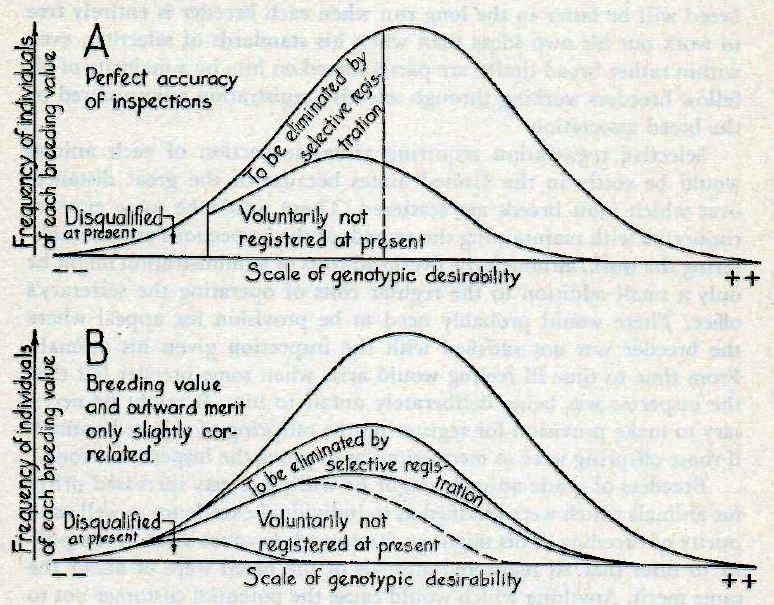
\includegraphics[width=\textwidth]{Figure_28.png}
    \caption{How the distribution of a population might be affected by selective
			 registration. Corresponding areas are the same size in the two diagrams.
			 The areas in each diagram are exclusive of each other. \textit{A}
			 presents the impossibly extreme case where the inspections could be
			 perfectly accurate. \textit{B} presents a more probable situation
			 where many mistakes would be made by the inspectors although they would be
			 right oftener than they would be wrong. If many were eliminated by the inspectors,
			 it might be necessary to register some of those voluntarily not registered at present.
			 Those would come from the areas just to the right of the dotted lines.}
    \label{fig:Lush_Figure_28}
\end{figure}
\index{Culling levels|)}

Both diagrams indicate that the animals not now registered include
many which are of higher breeding value than some of those which are
registered. It is probable that the average breeding worth of those registered
is higher than the average breeding worth of the eligible ones
which do not get registered, although the difference may not be as
extreme as is pictured here. Selective registration would increase the
intensity of selection for those genes which would usually make their
possessors appear more desirable to the inspectors. This would increase
slightly the rate of improvement in the breed, as far as mass selection
can do that and as far as the ideals set up to guide the inspectors are in
agreement with real merit. Whether the amount thus gained would be
sufficient to make selective registration worth the money and effort it
would cost is open to some doubt.

Selective registration would have some tendency to unify the standards
of selection within each breed, since each breeder would have to
be guided in part by the ideals of the inspectors. Those might not
always be superior to his own. This control over standards of selection
might do actual harm by preventing individual breeders from trying
out their own ideas as freely as they would like. To understand that,
one has only to imagine what would have happened if there had been
an official system of inspection in the Shorthorn breed when the Cruickshanks
were founding the``Scotch'' type or in the Poland-China breed
when Peter Mouw was forming the ``big type.'' The help which the
inspectors would give many breeders in their selections might more
than offset this. Moreover, the inspectors would probably be lenient
enough to allow each breeder considerable leeway for his own standards.
It remains an open question whether the average progress of the
breed will be faster in the long run when each breeder is entirely free
to work out his own ideas than when his standards of selection, even
within rather broad limits, are partly forced on him by a majority of his
fellow breeders working through selective registration administered by
the breed association.

Selective registration requiring visual inspection of each animal
would be costly in the United States because of the great distances
over which most breeds are scattered. There would be some expense
connected with maintaining the records of the inspections and administering
the work, although the overhead costs of administration might be
only a small addition to the regular costs of operating the secretary's
office. There would probably need to be provision for appeal where
the breeder was not satisfied with the inspection given his animals.
From time to time ill feeling would arise when some breeder felt that
the inspector was being deliberately unfair to him. It might be necessary
to make provision for registering the offspring of rejected animals
if those offspring were so meritorious as to prove the inspectors wrong.

Breeders of grade animals might be willing to pay increased prices
for animals which were certified as to individual excellence as well as to
purity of breeding. This might go far enough to cause some of the public
to infer that all registered animals of the breed were of about the
same merit. Anything which would cause the potential customer not to
study the animals before he makes his selection, or which would tend to
minimize attention to the breeder's reputation, has its possibilities of
doing harm. It seems unlikely that selective registration would be carried
far enough to make this danger important.

One commercial aspect of the situation is that some owners make
more strenuous efforts than others to sell males to other breeders of
purebreds. A certain amount of overhead in showing, advertising, and
sales efforts is required to sell any large fraction of the males produced.
In some cases those who make such efforts try hard to sell nearly all the
males they produce, while others make little effort to sell males except
to breeders of grades. The herds concerned usually do not differ that
much in real breeding merit. The adoption of selective registration
might restrict the efforts of those who are most active in selling males
more than it would those who are not now active at that. Doubtless
other unforeseen effects and complications will develop when selective
registration is put into practice. Any association attempting it will need
a trial period of several years to gain the experience necessary for making
the plan operate successfully when applied to the whole breed.

From 1942 to 1944, the American Jersey Cattle Club admitted bulls
to registry only if their paternal sisters or their dams had met certain
production requirements or if the sire was a ``star'' bull. The sire
becomes a star bull by his ancestors having met certain production
requirements or if at least ten of his paternal sisters and his dam have
been classified officially as to type and have scored high enough. There
are four grades of starring, the four-star bulls having the most promising
pedigrees, three-star bulls next, etc. In addition there are the
unstarred bulls which have not enough production or type ratings
among their near relatives to earn them even one star. Since 1944 the
compulsory features involved in selective registration. have been
dropped but the starring plan is retained. Since 1944 the Ayrshire association
lists progeny-tested sires in three classes of apparent merit but
what the breeder does with this listing is optional with him.

\section*{SELECTIVE REGISTRATION IN OTHER COUNTRIES}

Selective registration is practiced in many of the continental European
countries. The rules for operating the plan vary but in general are
somewhat as follows. The inspectors work under the direction of the
farmers' co-operative societies or of the breed association. In either case
there is usually some financial support from the government, accompanied
by a small amount of governmental supervision to see that such
money is spent in accordance with the laws appropriating it. The breed
association maintains tentative registry books and permanent registry
books. Soon after an animal is born it is entered in the tentative registry
and at an appropriate time an inspector certifies to this animal's individual
merit. It may then be placed in the permanent registry, or in
some cases it may remain in the tentative registry as long as it lives and
be placed in the permanent registry only after its death . Naturally the
animals are not inspected until they are grown or at least well along
toward maturity so that the inspector can be fairly certain of their
mature individuality. Tentative registry is therefore necessary to keep
the records straight. In the case of dairy cattle it is usually required that
females shall produce a minimum quantity of milk or fat before they
are finally placed in the permanent register and that males to be eligible
for the register must be out of cows which have met production
requirements higher than the minimum requirement which would
entitle cows to entry. Sometimes the inspection by the committee takes
place at the local fairs and sometimes the inspectors go from farm to
farm systematically or upon request.

The countries where these selective registration systems are in operation
are mostly countries where the breeds are native, and therefore the
ancestry of the majority of the commercial stock differs only slightly
from that of the pedigree stock. This makes more need for setting off,
by some special requirement or inspections, those animals good enough
to furnish future breeding stock than has been the case in the United
States, where most of the pure breeds have been imported and at first
differed greatly from the stock in the communities where they were
introduced. In most of the countries where selective registration is in
effect, the formal organization of the breed association occurred at a
comparatively recent date. This contributes something to the feeling
that there is no great gulf between the registered and the unregistered
animals. Usually provision is made for admitting to registry high grades
which are outstanding in their individual merit.
\nowidow

The following special items about selective registration in some
other countries may suggest the special conditions encountered and the
variety of ways adopted to meet them. They are by no means a complete
account of the registration systems in use. The details of those are
changed from time to time.\footnote{This is written in May, 1945.}

\textsc{Germany}. German animal breeding practices and customs of registration
were, of course, thrown into confusion by the war of 1914--18.
The cow-testing associations and similar organizations were again
operating on an extensive scale by 1924 or soon afterward. Since 1930
only cattle from herds which have been in cow-testing association work
have been eligible to be shown at the national exposition. Since 1934
and especially since 1936 the compulsory features of cow testing have
been greatly extended. In Hanover about 18 per cent of the cows were
tested voluntarily in 1934, but under compulsory testing this rose to 83
per cent by the beginning of 1937. The German animal breeding law
of 1936 brought about far-reaching control and compulsory inspection
(Korung) of all classes of breeding stock. In many cases only one or two
breeds could be kept in each district. This extended to sires used only
in private herds, as well as to sires which were offered for public service.
This system was not in operation long enough before the next war to
demonstrate what effects it actually would have.

\textsc{Holland}. The Netherlands Herdbook Association\footnote{The Friesian
Cattle Herdbook Association (with headquarters at Leeuwarden) has a slightly
different procedure.} at the Hague maintains four kinds of herdbooks: the
calfbook, where service certificates and \index{Birth certificates}birth certificates are filed in
order to keep the records of ancestry straight; the herdbook proper, to which
animals are admitted on mature inspection; the advanced register for recording
production; and the register of proved sires. The filing of service certificates
soon after breeding is compulsory. The filing of the birth certificate must take
place within a few weeks after the birth of the calf. Females are
inspected and scored for entry into the herdbook proper soon after they
drop their first calf. A score of 75 points out of a possible 100 is necessary
for registration. Recording milk and fat production is not compulsory,
but bulls are not accepted for registry unless they are from
tested dams. Bulls are inspected and scored soon after they are 12
months old, before they go into service, but must be scored again after
they are 24 months old. If a bull is accepted as a yearling but is rejected
at the two-year-old scoring, the owner is allowed 30 days as a reasonable
time in which to get another bull. All services made by the rejected bull
more than thirty days after his rejection are treated as though the bull
were a grade, but services made prior to that are accepted for purposes
of registration. The inspection is so severe that about 55 per cent of all
bulls offered for inspection are rejected. There is, of course, no way of
judging how much selection the breeders have already practiced in
deciding which bulls shall be offered for inspection.

\textsc{Switzerland}. In Switzerland the physical conditions, especially the
summer use of mountain pastures far from the home villages and the
small size of many of the herds, compel more co-operation among
breeders than is usual in the United States. Bulls must be shown at the
large regional fairs for classification if the purchasers are to be eligible
to receive the payments which the government provides for stimulating
the use of improved sires. Such payments and other considerations are
important enough that almost all bulls get shown at these large regionai
shows. Frequently as many as 1,300 Brown Swiss bulls are shown at one
time at the largest fair. The cows are offered for inspection at the local
or village fairs. Cows are scored during their first or second lactations,
and those scores are printed along with their pedigrees in the printed
herdbooks. The advanced registry records not only how much milk and
fat the cow gave, but also how many hours she worked at draft purposes
during the year. A considerable fraction of the Swiss cattle are used for
milk, work, and beef, thus being in a sense triple-purpose cattle. Special
stress is laid on longevity and regularity of breeding . Each cow which
produces at least six living calves in the space of eight consecutive years
is given a special distinguishing mark in the printed herdbook.

\textsc{Denmark}. In Denmark there is widespread co-operation among
farmers for many purposes, and the co-operative societies conduct the
pedigree registration and other means of livestock improvement. Breed
registry societies, such as those in the United States and Britain, do not
exist. A committee of the union of co-operative societies directs the registration
policies as the board of directors of a breed association would
do in the United States. Of course, most members of this committee are
breeders themselves or have in some other way made themselves thoroughly
familiar with the practical problems which breeders encounter.
Hence, the conduct of registration is not very different from that in the
United States; but the committee members are responsible to the farmer
co-operative societies, that is, to the customers who will use the
improved breeding stock being produced. It has been agreed that 500
cows registered per year is a large enough number to supply the real
needs of the breeders and farmers. The animal husbandry \textit{consulents}
\footnote{Employees of the co-operative societies who provide technical
advice on livestock matters, somewhat as county agricultural agents do in
the United States, and also act to some extent as the business agents for
their co-operatives.}
nominate something like twice that number of cows. Then the central
committees consider the available data concerning these and discard
those which seem least worthy until the number is reduced to 500. Cows
rejected one year can be nominated again and perhaps accepted in a
later year. No cow is considered until she has been in milk at least three
consecutive years. No matter what her age when nominated, her actual
uncorrected fat production must have averaged more than 400 pounds
per year ever since she first freshened. The national committee in
charge of swine breeding supervises the registration of swine. Registrations
are accepted only for animals bred at the state-recognized swine
breeding centers. Those are farms where the breeders have complied
with certain regulations, including sending each year to the testing stations
half as many test litters as they have sows in their herds.\footnote{Lush,
Jay L. 1936. Genetic aspects of the Danish system of progeny-testing swine.
Iowa Agr. Exp. Sta., Res. Bul. 204.} At the testing stations these test litters
(of four pigs each) are fed under standard conditions, and the rates and
economy of gain are recorded. When each pig reaches 200 pounds, it is
slaughtered at a nearby bacon factory and its dressing percentage and the type,
conformation, and quality of its carcass are measured and scored. Also, each
breeding center is inspected twice each year by a committee which scores it
for: (1) management and general appearance of the farm, (2) conformation of the
breeding animals, (3) fertility of the breeding animals, (4) efficiency in the
use of feed by the test pigs from this center, and (5) slaughter quality of the
test pigs from this center. The considerable costs of the swine improvement plans
are mainly borne by the co-operative bacon factories. The plans are thus directed
and financed indirectly by the customers who buy the improved breeding stock and
not by the breeders who produce it. The government makes a small financial
contribution to part of the work and extends legal authority where needed to the
co-operative societies or to the co-operative bacon factories but does
not itself take an active part in directing the work. Exhibiting at the
fairs is not compulsory, but a large part of the breeders do that. The
classification made at the fairs is entered in the herdbooks or other records
pertaining to those animals, so that most pedigrees have in them
considerable information about the type classification of the ancestors,
especially of the sires. The central committees specify in detail the kind
of records which each stockman, who aspires to be called a breeder,
must keep. The committees or their representatives inspect those private
herdbooks at certain intervals for accuracy and completeness. In
some cases the owner is not permitted to make the entries himself but
must keep the notes and papers concerning each event until the consulent
comes on one of his regular visits, verifies them as well as he can,
and makes the proper entries. This supervision and uniformity give the
private herdbooks a semiofficial standing and make it unnecessary for
the central committee to keep birth certificates or other records of that
kind on animals not yet admitted to the national herdbooks.

These details will show something about how widely the pattern of
selective registration may vary from country to country according to
circumstances. If selective registration is adopted in the United States,
still other devices will be needed to adapt it to the local needs and
conditions.

\section*{AMERICAN APPROACHES TO SELECTIVE REGISTRATION}
\index{Breed associations|(}

The Standardbred horse is an American breed which takes its mime
from the fact that in its early history animals must have been able to
trot a mile in 2 minutes and 30 seconds or pace a mile in 2 minutes and
25 seconds before they could be registered. The Brahman Cattle Breeders
Association (founded in 1924 and operating mostly in the coastal
regions of Texas and Louisiana) requires inspection of animals before
they are accepted for registry. The scores and other descriptive comments
concerning each animal are filed with its registration in the
secretary's office. No herdbook has yet been published. When the Jersey
breeders established their Register of Merit in 1903, many of the cows
were measured and scored as to type by some member of a group of
about 19 authorized judges. These scores were not used, however, to
determine eligibility for registry. They were intended to furnish evidence
about the relation between type and production. Perhaps also
some of the breeders then feared that unfortunate results would follow
if the Register of Merit were allowed to operate with no attention at all
to type.

\textsc{Disqualifications}. Many breeds have certain absolute disqualifications
which are a bar to registry, even though the breeding is of
undoubted purity. Thus, an Aberdeen-Angus which is red is not now
eligible to registry; although red cows were eligible until about 1915.
Red Aberdeen-Angus steers may still be registered to compete for prize
money at the fairs. Neither is a red and white Holstein-Friesian nor one
with black completely encircling the hoof-head eligible to registry. Most
of these absolute disqualifications concern deviations from the peculiar
type of that breed, which usually means details of conformation or
color not directly affecting their usefulness as producers of meat, milk,
eggs, wool, or power. No association will knowingly register an animal,
either male or female, which is known to be a nonbreeder, except in the
case of fat animals and geldings to be exhibited at shows. In none of the
cattle breeds can a heifer born twin with a bull be registered until proof
is furnished that she is fertile. This restriction is based upon the common
experience that most such heifers \index{``Free-martin''}(``free-martins'') will be barren.
Years ago some of the breeds had rules against registering offspring
from dams which had formerly produced crossbred young to the service
of grade sires or sires of other breeds. Only a few breeders actually professed
a belief that this would affect the breeding value of subsequent
purebred offspring (``telegony'')\index{Telegony}, but the rule was placed in the by-laws
of many associations on the long chance that there might be something
to it. In 1924 it was removed from the by-laws of the last large association
(a sheep one) which had had this rule. Breeders of dogs are reputed
to believe more in telegony than breeders of other livestock.

\textsc{Age Restrictions}. Many American breed associations levy an extra
charge on registrations not made until after the animal passes a certain
minimum age. In some breeds the animals cannot be registered at all
after they pass a certain age. One reason for this is to complete the registration
before the breeder loses or forgets some of the facts in the case.
The opportunity for fraud is also diminished by having the registration
made promptly. More animals are registered than if registration could
be postponed indefinitely without penalty. One unfortunate result is
that some animals are registered young which would not be registered
if the breeder could wait until he could see them as mature animals. A
plan which promises to combine the advantages without the disadvantages
of early registration is ``deferred registration'' such as that in effect
with the Guernsey, Jersey, and Ayrshire breeds. Under this plan the
breeder files a birth certificate soon after the calf is born. The fee for
this is small. This birth certificate entitles the breeder to defer final
registration until the animal is mature, without incurring any penalty
for lateness.

\textsc{Voluntary Plans}. The voluntary Herd Classification plans of the
dairy cattle registry associations in the United States embody some
selective registration in the fact that the registration certificates must be
surrendered on animals classified as poor and that bulls out of cows
classified as fair are not eligible to registry. The Herd Classification
plan also records the animals in several different classes of individual
merit, so that one who does not know the animals may learn what the
classification committee thought of their individuality. The type classification\index{Type classification}
is printed, after the name and number of each classified animal,
in the various printed herdbooks. This puts more meaning in
pedigrees in which these classified animals appear.

A feature of selective registration in the Herd Improvement Registry
of dairy cattle is that the breeder who surrenders the registration
certificates for his poorest producers is entitled to have those omitted
from the published average for the production of his herd. The extent
to which this is actually being done may be seen from the fact that, in
the first 13 volumes of the Holstein-Friesian Herd Improvement Registry,
14,733 certificates of registry were surrendered voluntarily. This
was 10.3 per cent of the total number of cows on test. Of course, some of
these surrendered certificates were for cows already dead or barren.
Even so, the figures indicate some selective registration against the
least productive animals even after the expense of registration has
been met.

The Ayrshire Association registers bull calves under six months old
for half price if the sire and dam, or the dam and paternal grandam, or
all four grandparents are in the Ayrshire Advanced Registry.

Such individual registration of poultry as exists is mostly connected
with records of performance in such a way that it is selective.

\textsc{Abandoned Plans}. In 1889--91 the Holstein-Friesian Association
paid bounties of \$5 each for the castration or vealing of bull calves
which were eligible to registry. This was a systematic attempt to induce
the breeders to discard their ordinary and inferior male calves. The
plan was discontinued because nearly as many bull calves were registered
while the plan was in effect as before, and it was a heavy drain on
the association treasury, more than \$20,000 being thus expended in the
three years it was in effect.

The Hereford association in 1895 and 1896 had a rule that 10 per
cent of all applications for registry of bulls from each herd should be
rejected, but the Secretary had no guide as to which ones those should
be. The ruling was repealed in 1897.

\section*{SUMMARY}

Selective registration is a form of official mass selection which consists
in preventing individuals deemed inferior from leaving any registered
descendants. Such selection cannot do any more than the individual
breeder could; it may do more than he would if left entirely to
his own initiative. Collective wisdom, as imparted by the inspector,
might help the less well informed and might be of considerable help to
the customer. Probably it could not rise to the level of the ablest individual
breeder's ability.

Selective registration is widely practiced in many foreign countries,
but some of their conditions are distinctly different from those in the
United States.

Some of the American associations are experimenting with devices
embodying some voluntary principles of selective registration. Doubtless
these will be carried farther if they are found satisfactory and if the
problem of expense can be solved.
\index{Breed associations|)}

\section*{REFERENCES}
\begin{hangparas}{0.5in}{1}%
American Jersey Cattle Club. 1941. Selective Registration.

Gardner, Malcolm H. 1932. Selective herd-hook registration. Holstein-Friesian
World. 29:411--12 and 428.

Van den Bosch , I. G. J . 1930. The scoring system in the Netherlands. Holstein-Friesian
World, 27:337 et seq.

---. 1930. The Holstein industry in America. Holstein-Friesian World, 27:283.

Wriedt, Christian. 1930. Heredity in livestock. (Especially pp. 151--67). New York:
The Macmillan Company.
\end{hangparas}
\index{Selective registration|)}
\chapter{Type and Production Records}
\label{cha:Lush_Chapter_17}
\index{Type and production|(}

Breeders pay attention to outward conformation in making their
selections for two reasons. In the first place, they may want a certain
type because it has a market value. If a market demand exists for a certain
type, the breeder may care little whether that type really will furnish
to his customers the maximum profit or other satisfaction. The fact
that they want it and are willing to pay for it is the thing of immediate
practical importance to him. In the second place, breeders may believe
that type and productiveness are closely enough correlated that if one
selects for type he will get at least part of the productiveness he wants.

In many cases, especially among meat animals ready for market, a
certain conformation not merely indicates production but actually
comes close to being production, since the desired production is largely
a matter of sizes and proportions of various parts. At the other extreme
are cases where the desired production depends far more on the quality
and rates of physiological processes than it does on the sizes and shapes
of organs or parts which can be judged on the live animal. The closeness
of the correlation between type and production may be of any
degree ranging from almost perfect in such a case as the width of the
loin or thickness of the round on fat steers, through such relations as
may possibly exist between width of head and width of body, to correlations
which are practically zero. An example of a correlation which was
once thought to be high but has since been found to be practically zero
is the relation which a half century ago was widely supposed to exist
between the escutcheon of a cow and her producing ability.

Reliance on type as a means of estimating productive ability may
be necessary when reliable records of production are not available.
Production records on most animals come slowly and expensively.
Sometimes, as in poultry and dairy cattle, they are not available on both
sexes. Even where production records can be fairly simple and complete,
as in the case of cows and hens, it is still true that many purebred
animals do not have their production recorded. The situation is still
less satisfactory among meat and work animals, where productivity is
not easily nor completely measured. A breeder often has an opportunity
to buy an animal on which no production record has been made, or he
may have to sell some of his young stock before they are old enough
to have production records. Such a breeder, even though he has more
faith in production records as indicating an animal's productivity than
in conformation as a similar index, none the less wants to make as much
use as he can of the animal's conformation in estimating its probable
productivity.

Type has some sale value in all classes of livestock. In extreme cases
beauty may be the main object. This is often encountered in ``pet and
fancy stock,'' such as rabbits, dogs, pigeons, and guinea pigs, and is a
prominent feature of some of the larger livestock such as saddle and
coach horses. If the breeder's customers center their demand on type, he
is of course interested mainly in that, and in productiveness only in
that his animals should remain healthy and fertile. To appear healthy
is, in most cases, an important part of the breed ideal for type also. If
his customers are looking for productiveness regardless of beauty, the
breeder is interested in type only as it may help him get that productiveness
more surely and quickly than if he did not pay attention to
type.

The stockman usually wants lifelong productiveness in each animal
rather than a maximum single record from each, although the advertising
value of an extremely high record may sometimes mean more financially
to a breeder than a higher average record\index{Lifetime Averages} which does not become
phenomenal in any one year. A single production record is not a perfect
index of such life productivity, as was emphasized in chapter \ref{cha:Lush_Chapter_13}. The
question of how much attention to pay to type and how much to pay to
production records in selecting for lifetime productivity is, therefore, a
question of comparing and combining two indicators, neither of which
is perfectly accurate. Yet it would be a rare coincidence if the usefulness
of the two happened to be exactly equal. The principles of estimating
an unknown quantity from two known quantities which are partly
correlated with it are such that a slightly more accurate estimate may
usually be made by using both the known quantities than by using the
more accurate of them alone, although the best proportion in which to
weight the two is much affected by their relation to each other.

Each intermediate step weakens the effectiveness of selection. Thus,
if we want to select for quality \textit{x}, and it is correlated
imperfectly with \textit{w}, we will not come so close to getting
\textit{x} by selecting \textit{w} as we would if we could select
\textit{x} directly.\footnote{As a numerical example, Rasmusson has
shown (1930, \textit{Nordisk Jordbrugsforskning}, pp. 247--55) that
even if the correlation between \textit{x} and \textit{w} is .8, one
wishing to select a certain number of individuals which excel the
population average in \textit{x} by at least one standard deviation
would need to examine 7.8 times as many if he selects them indirectly
by looking for \textit{w} as he would if he could select them directly
by examining them for \textit{x}.} If \textit{x} cannot be observed
directly but is rather closely correlated with \textit{y} and not so
closely with \textit{w}, we would come nearer getting the value of
\textit{x} we want by selecting for \textit{y} than by selecting for
\textit{w}. Unless \textit{w}'s correlation with \textit{x} is
altogether due to \textit{w}'s correlation with \textit{y}, we would
come still nearer to getting the desired value of \textit{x} by
selecting for both \textit{y} and \textit{w}; but the proper amount of
attention to be given to \textit{y} or to \textit{w} would depend upon
how closely they were correlated with \textit{x} and with each other.
The guiding principle on this subject is that every needless intermediate
step in selection should be avoided as far as possible but that a little
is usually gained by paying some attention to other things besides the one
which is most closely correlated with productivity. The very real danger
in that is that one will pay so much attention to these minor things that
he cannot pay enough attention to more important things which are more
closely correlated with lifelong productivity.

\section*{THE CORRELATION BETWEEN TYPE AND PRODUCTION}

In most actual studies of the correlation between type and production
the correlation between one estimate of type or conformation and
one production record of each individual in the population studied was
measured. A few samples of those are mentioned in the following paragraphs.

When official testing began in the Jersey breed, certain judges
inspected and scored the cows admitted to the Register of Merit.
Gowen studied these data to see what correlation existed between the
scores and the production records. Most of the correlations between the
scores for each individual point of conformation and the actual production
records of those cows were of about the magnitude of $- .07$ to $+ .19$.
The correlation between the production record and the total
score of the cow ran somewhat higher, since it took into account all of
the points scored. When the study was confined to the scores turned in
by the nine judges (out of the nineteen recognized ones) whose scores
most closely agreed with the milk yield of the cows, the correlation
between their total score and the milk yield was $+ .38$. While this is a
real correlation, it was obtained only after discarding the scores of half
of these men who were believed by the association to be competent to
score the cows.

In similar studies on early Holstein-Friesian records Gowen used
measurements made on some of the first officially tested cows.
Table~\ref{tbl:Lush_Table_14} presents the correlation coefficients
he found between the seven-day milk yield and various body measurements
and weights.

The maximum correlation between yield and any body measurement
was .36. The correlations found were real and of some use in
selecting the high producers, but they were by no means as high as the
correlations between different records made by the same cow. A considerable
part of these correlations with measurements resulted from differences
in general size. Within a breed the largest cows tend to be the
heaviest producers and naturally tend also to have the largest measurements.

Engeler's study\footnote{1933. Die Ergebnisse statistischer Auswertung
40-j\"ahriger Herdebuch-Aufzeichnungen beim schweizerischen Braunvieh.
Bern: Verbandsdruckerei A. G.} of the yields of 455 Brown Swiss cows and their
scores when they were inspected for registration showed a correlation
of only $+ .04$. In another study 3 of 138 cows\footnote{Schweizerische Landw.
Monatshefte 19, No. 6, 1941.} in one herd he found a correlation of $+ .32$
between milk yield and score.

\begin{table}[htbp]
	\centering
	\caption{\textsc{Correlation Coefficients Between Seven-Day Milk Yields and Certain Aspects
of Conformation, Age Being Constant (After Gowen)}}
	\label{tbl:Lush_Table_14}
	\begin{tabular}{lc}
		\hline
		\hline
		 													& Correlation \\
		Characters Correlated								& Coefficient \\
		\hline
		365-day milk yields in different lactations			& .66 \\
		7-day with 365-day milk yield (same lactation)		& .60 \\
		7-day with 365-day milk yield (different lactation)	& .46 \\
		Weight with 7-day milk yield						& .42 \\
		Body length with 7-day milk yield					& .36 \\
		Body girth with 7-day milk yield					& .25 \\
		Body width with 7-day milk yield					& .28 \\
		Hip height with 7-day milk yield					& .24 \\
		Shoulder height with 7-day milk yield				& .22 \\
		Rump length with 7-day milk yield					& .18 \\
		Thur! width with 7-day milk yield					& .01 \\
		\hline
	\end{tabular}
\end{table}

In dairy cattle there have been several studies of show-ring placings
and production records, where both were known. Because only a small
range of types was included -- no really poor types would be among
those for which the placings were recorded -- such studies throw little
light on the correlation between type and production. They demonstrate
that show animals can produce well, but so might many others if
tested under the same circumstances.

A more suitable basis for studying the correlation between type and
production is in such data as the Holstein-Friesian Herd Classification.
Table~\ref{tbl:Lush_Table_15} shows a summary of such data.\footnote{As
of October, 1942. The records are on a thrice-a-day mature basis and include
the first 365 days of the lactation.} The figures show that type
and production do tend to go together in this population. On the average
the fat production increased 24.6 pounds with each grade the cow
was higher in the type classification\index{Type classification}. The correlation between the two
is a little less than $+ .2$. That leaves plenty of opportunity for very
high producers occasionally to be of poor type and for some animals of
high type to be poor producers. The correlation in the general population
of dairy cattle is probably a little higher than this, since, in the
herds submitted for classification, most of the cows thought by their
owners to be ``Fair'' or ``Poor'' in type already would have been culled
unless their production was unusually good. On the other hand, part of
the apparent correlation may have come about because large size gives
an advantage, both in classification and in production. Also, the classification
may have been influenced in some cases by knowledge which the
classifying officer had of the cow's prior production.

\begin{table}[htbp]
	\centering
	\caption{\textsc{Average Herd Test Records of Holstein-Friesian Cows as Classified for Type
Under the Herd Classification Plan}}
	\label{tbl:Lush_Table_15}
	\begin{tabular}{L{2.5cm}|R{3cm}|R{1.75cm}|R{1.75cm}}
		\hline
		\hline
		Type						& 					& \multicolumn{2}{c}{Average Production} \\
		\cline{3-4}
		Classification				& Number of Cows	& Milk		& Fat \\
		\hline
		Excellent					& 261				& 17,215	& 601 \\
		Very good					& 1,377				& 15,988	& 554 \\
		Good plus					& 2,213				& 15,754	& 544 \\
		Good						& 2,138				& 14,960	& 514 \\
		Fair						& 426				& 14,316	& 488 \\
		Poor						& 25				& 12,612	& 431 \\
		\hline
	\end{tabular}
\end{table}

Table~\ref{tbl:Lush_Table_16} shows the summary of such data on Jersey cows
to April, 1946 on a twice-a-day 305 day basis. The regression of fat production
on type -- the average increase in fat production with each increase of
one grade in type classification -- was 12.8 pounds which is only a little
less than the 24.6 from the Holstein data when allowance is made for
lactation length and times milked per day.

\begin{table}[htbp]
	\centering
	\caption{\textsc{Average Herd Test Records of Jersey Cows Which Were Also
Classified Officially for Type}}
	\label{tbl:Lush_Table_16}
	\begin{tabular}{L{3cm}|R{3cm}|R{3cm}}
		\hline
		\hline
		Type Classification			& Number of Cows	& Average Fat Production \\
		\hline
		Excellent					& 801				& 483 \\
		Very good					& 4,213				& 460 \\
		Good plus					& 6,060				& 448 \\
		Good						& 2,700				& 434 \\
		Fair						& 369				& 420 \\
		\hline
	\end{tabular}
\end{table}

Engeler's conclusion from studies in Switzerland is: ``Form, production,
and health are not so closely related that they can be substituted
for each other as bases for selection. These three characteristics are to a
high degree independent of each other and to a high degree are transmitted
independently to the offspring. The goal of selection consists
in preferring those animals which to the fullest extent possess all three
characteristics, phenotypically as well as genotypically.''

On poultry several studies have been made of the relation between
body measurements and production or of the success which a man
actually attains in attempting to cull out the poorest producers from
each lot, dividing them into two groups and noting their production
immediately after the culling. In the culling demonstrations the apparently
high success is largely the result of immediately preceding conditions,
whereby the man doing the culling is able to identify those which
are laying at that time. Since the test pens are not kept for a full year
afterward, he seems to have been remarkably successful in picking out
the poor producers. It is somewhat the same situation as if one were to
go to a dairy farm and rank the cows according to his estimate of their
milk-producing ability. If his rankings were then compared with the
cows' actual productions in the following week or two weeks, he would
seem to have been remarkably successful; but much of this success
would be due to the fact that he could tell which cows were dry and
which were recently fresh at that particular time! The available evidence
makes it seem doubtful that the relation between productiveness
and conformation is really any closer in poultry than it is in dairy cattle.

Studies of the relation between weight, conformation, and pulling
ability in draft horses have shown (Rhoad) correlations of about the
magnitude of $+ .23$ to $+ .35$ between different measurements and ability
to pull and + .45 between weight and ability to pull. However,
nearly all of the correlation between measurements and ability to pull
seemed to be an indirect result of general size, because the relation
between these measurements and pulling ability within groups of
horses which were all of the same weight was practically zero. In a similar
study Brandt found that weight, age, and five measurements had a
multiple correlation of .47 with maximum pull. Most of this seemed to
depend on weight and height.

Studies of individual beef cattle have been less frequent because
there is no one measure which comes as near expressing their real productivity
as the actual production records of dairy cattle, poultry, and
draft horses do in those cases. The studies which have been made show
moderate or low correlations except for anatomical traits, such as fullness
of round, which can be estimated closely when judged in the live
animal before slaughter. There have been many studies of commercial
grades of groups of feeder steers as related to their subsequent performance
in the feedlot. Usually the steers of the lower grades gain about as
rapidly as those in the higher grades, but they sell at a lower price.
Whether they are equally profitable to the feeder depends mostly on
whether he can buy them at a low enough price. Because of the lower
sale price, the lower commercial grades are less profitable to the
man who breeds them.

Studies of type and production in sheep have been more numerous
but have dealt mostly with the production of wool or with the feeding
qualities of groups of lambs from the crossing of various breeds. Questions
of type are often the subject of discussion among breeders of Merino
and Rambouillet sheep\footnote{See Texas Bul. 657. Also Michigan Quart.
Bul. 26:31--33.} and Angora goats.

Several experiment stations have conducted swine type tests which
have shown differences in the rates of gain and in the kind of meat produced
by swine of types varying from ``very chuffy'' to ``extremely
rangy.'' Studies of the ability of men to predict which pigs would make
maximum gains have generally shown correlations of something
around $+ .4$ to $+ .7$ between the estimate and the actual individual
gain. These high correlations (compared with much lower ones on
steers) are generally reduced to somewhere near the level of $+ .15$
to $+ .30$ when corrected for differences in initial weight.
Greve\footnote{Zeit. f. Z\"ucht., Reihe B., 46:91, 1938.} studied
eight different measurements on 205 sows of the Hoya breed near Hanover
in Germany and concluded: ``All the results show that it is not
possible by using body measurement to find which sows have high
breeding productivity.''

Summarizing the actual evidence on the correlation between individual
type and individual production, there is no complete analysis of
the problem in any class of livestock; but the nearest approach to that
has been in dairy cattle or poultry. In general, these studies have established
the existence of correlations between type and production; but
such correlations are generally much lower than the correlation
between one production record and another production record of the
same animal. The conclusion seems inevitable that if one is interested
mainly in production he should pay much more attention to production
records than to estimates of type, although it does not follow that
he could afford to neglect type altogether. An actual production record
is not quite a perfect indication of the lifelong production which is.
actually wanted. The emphasis placed by many men on outward evidences
of health and ``constitution'' may have some justification in the relation
of those to lifelong productivity. Many of the breeder's decisions
must be made before he can know from actual experience what
that animal's lifelong production will really be. Where type has any
direct relation to lifelong productivity, the latter can be predicted more
accurately by taking into account both type and production records
than by using either alone, but the one which is least closely related to
lifelong production should be given much less emphasis.

\section*{SUMMARY}

A breeder may pay attention to type merely because it will add to
the market value of the animals he expects to produce. Aesthetic considerations
have much to do with the commercial value of some kinds of
animals.

A breeder may also pay attention to type because he believes it to be
a useful indicator of the lifelong productivity of the animal. Such indicators,
even though not as reliable as production records, would be
useful under a variety of circumstances actually encountered, especially
among animals on which production records are lacking.

What is wanted is lifelong productivity. A single production record
is not quite the same thing, although in most cases it is a more accurate
indicator of lifelong productivity than is the individual's type, if either
were to be considered alone.

Where type is related directly to productivity, a more accurate estimate
of productivity can be made by taking type and the available
production records both into account than by considering either alone,
but there is danger of paying too much attention to the less accurate of
the two indicators.

The practical problem confronting the breeder is to give the proper
amount of attention to each. If he pays too much attention to type, the
selection he can practice for production is automatically made less
intense.

\section*{REFERENCES}

There are many published studies which bear in part on this topic.
The following ones will illustrate the methods of study and will indicate
the kind of conclusions which are generally drawn. This list is not
complete but is representative of the more recent ones written in English
and readily accessible to most students in the United States.

\noindent
\textbf{For Dairy Cattle:}

\begin{hangparas}{0.5in}{1}%
Aldrich, A. W., and Dana, J. W. 1917. The relation of the milk vein system to
production. Vermont Agr. Exp. Sta., Bul. 202.

Brody, S., and Ragsdale, A. C. 1935. Evaluating the efficiency of dairy cattle. Missouri
Agr. Exp. Sta., Bul. 351.

Copeland, Lynn. 1938. The old story of type and production. Jour. Dy. Sci. 21:295--
303.

Gaines, W. L. 1931. Size of cow and efficiency of milk production. Jour. Dy. Sci. 14:
14--25.

Garner, F. H. 1932. A study of some points of conformation and milk yield in Friesian
cows. Jour. Dy. Res., 4:1--10.

Gowen, John W. 1924. Milk secretion. pp. 32--49.

---. 1923. Conformation and milk yield in the light of the personal equation
of the cattle judge. Maine Agr. Exp. Sta., Bul. 314.

---. 1925. The size of the cow in relation to the size of her milk production.
Jour. Agr. Res., 30:865--69.

---. 1926. Genetics of breeding better dairy stock. Jour. Dy. Sci., 9:153--70.

---. 1931. Body pattern as related to mammary gland secretion. Proc. Nat.
Acad. of Sci., 17:518--23.

---. 1933. Conformation of the cow as related to milk secretion. Jour. Agr.
Sci., 23:485--518.

Swett, W. W.; Graves, R. R.; and Miller, F. W. 1928. Comparison of conformation,
anatomy, and skeletal structure of a highly specialized dairy cow and a highly
specialized beef cow. Jour. Agr. Res., 37:685--717.
\end{hangparas}

\noindent
\textbf{For Poultry:}

\begin{hangparas}{0.5in}{1}%
Bryant, R. L., and Stephenson, A. B. 1945. The relationship between egg production
and body type and weight in Single Comb White Leghorn hens. Va. Agr. Exp. Sta.,
Tech. Bul. 96.

Juli, M. A.; Quinn, J. P.; and Godfrey, A. B. 1933. Is there an egg-laying type of the
domestic fowl? Poul. Sci., 12: 153--62.

Knox, C. W., and Bittenbender, H. A. 1927. Correlation of physical measurements
with egg production in White Plymouth Rock hens. Iowa Agr. Exp. Sta.,
Res. Bul. 103.

Marble, D. R. 1932. The relationship of skull measurements to cycle and egg
production. Poul. Sci., 11:272--78.

Miller, M. Wayne, and Carver, J. S. 1934. The relationship of anatomical measurements
to egg production. Poul. Sci., 13:242--49.

Sherwood, Ross M., and Godbey, C. B. 1928. Construction of score card for judging
for egg production. Poul. Sci., 7:263--74.

Waters, Nelson F. 1927. The relationship between body measurements and egg production
in Single Comb White Leghorn fowls. Poul. Sci., 6:167--73.
\end{hangparas}

\noindent
\textbf{For Horses:}

\begin{hangparas}{0.5in}{1}%
Brandt, A. E. 1927. Relation between form and power in the horse. Trans. Amer.
Soc. Agr. Eng., 21:PM---3--4.

Dawson, W. M. 1934. The pulling ability of horses as shown by dynamometer tests
in Illinois. Proc. Amer. Soc. An. Prod. for 1933, pp. 117--21.

Dinsmore , Wayne. Learn to judge your horses and mules. Leaflet No. 196 of the
Horse Association of America.

Laughlin, H. H. 1927. The Thoroughbred horse. Carnegie Institution of Washington.
Yearbook No. 26, pp. 56--58. (See preceding and following yearbooks
for other short notes on this.)

Rhoad, A. O. 1929. Relation between conformation and pulling ability of draft
horses. Proc. Amer. Soc. An. Prod. for 1928, pp. 182--88.
\end{hangparas}

\noindent
\textbf{For Swine:}

\begin{hangparas}{0.5in}{1}%
Bull, S.; Olson, F. C.; Hunt, G. E.; and Carroll, W. E. 1935. Value of present-day
swine types in meeting changed consumer demand. Illinois Agr. Exp. Sta.,
Bul. 415.

Nordby, J.E. 1932. Type in market swine and its influence on quality of pork. Idaho
Agr. Exp. Sta., Bul. 190.

Scott, E. L. 1930. The influence of the growth and fattening processes on the quality
and quantity of meat yielded by swine. Purdue Agr. Exp. Sta., Bul. 340.
\end{hangparas}

\noindent
\textbf{For Beef Cattle:}

\begin{hangparas}{0.5in}{1}%
Black, W. H.; Knapp, Bradford, Jr.; and Cook, A. C. 1938. Correlation of body
measurements of slaughter steers with rate and efficiency of gain and with
certain carcass characteristics. Jour. Agr. Res. 56:465--72.

Hultz, F. S., and Wheeler, S. S. 1927. Type in two-year-old beef steers. Wyoming
Agr. Exp. Sta., Bul. 155.

Lush, Jay L. 1931. Predicting gains in feeder cattle and pigs. Jour. Agr. Res.,
42:853--81.

---. 1932. The relation of body shape of feeder steers to rate of gain, to
dressing per cent, and to value of dressed carcass. Texas Agr. Exp. Sta., Bul.
471.
\end{hangparas}

\noindent
\textbf{For Sheep:}

\begin{hangparas}{0.5in}{1}%
Bosman, V. 1933. Skin folds in the Merino sheep. S. African Jour. Sci., 30:360--65.

Cole, C. L. 1943. Type selection vs. record of performance in sheep breeding. Quart.
Bul. Michigan Agr. Exp. Sta. 26:31--33.

Hultz, Fred S. 1927. Wool studies with Rambouillet sheep. Wyoming Agr. Exp. Sta.,
Bul. 154.

---. 1935. A five-year study of Hampshire show sheep. Wyoming Agr. Exp.
Sta., Bul. 207.

Jones, J. M.; Dameron, W. H.; Davis, S. P.; Warwick, B. L.; and Patterson, R. E.
1944. lnfluence of age, type and fertility in Rambouillet ewes on fineness
of fiber, fleece weight, staple length, and body weight. Texas Agr. Exp. Sta.,
Bul. 657.

Joseph, W. E. 1931. Relation of size of grade fine-wool ewes to their production.
Montana Agr. Exp. Sta., Bul. 242.

Spencer, D. A., and Hardy, J. I. 1928. Factors that influence wool production with
range Rambouillet sheep. USDA, Tech. Bul. 85.
\end{hangparas}
\index{Type and production|)}
\chapter{Breed Type}
\label{cha:Lush_Chapter_18}
\index{Breed purity|(}
\index{Breed type|(}
\index{Deviations from type|(}
\index{``Fancy points''|(}
\index{Percentage of blood|(}
\index{``Pet and fancy stock''|(}

Breed type means the complex of external characteristics which is
typical of a breed or is considered ideal for that breed. The term is often
used in distinguishing one breed from another breed used for much the
same purpose. Many ingredients of breed type are conspicuous details
of conformation and color which have no relation to the economic productivity
of the animals. Examples are the shape of horns in cattle, the
dish of face and size and shape of ear in swine, color of face and shape
of ear in sheep, and color generally. It is those features of breed type
which are the subject of this chapter.

Attention is paid to breed type mainly because it is a ``trademark''
which is some additional evidence that the animal really conforms to
the ideals of the breed. Probably the men who breed purebred animals
average somewhat higher in honesty than men in most other lines of
work, since the foundation of the pedigreed livestock business is the
honesty of the men who sign their names to the pedigrees. Without
general honesty on this point purebred animals could not command the
premium they do. Yet there will always be a few mistakes and frauds.
The existence of a definite breed type, especially if that is a combination
of characters hard to obtain without absolutely pure breeding, is
one check upon errors in registration. If a breed has a type of this kind,
an animal deviating markedly from that type will be regarded with suspicion.
From this point of view the breed type which is the hardest to
attain or which is the most easily upset in crosses is the most highly
prized. This often goes to extremes in the case of ``fancy stock,'' such as
pigeons, rabbits, or dogs, the desired type or standard being kept just
high enough or changed just often enough that only a small proportion
of the breed attain it.

Of course, breed type also is a matter of beauty to the men who have
long been breeding and admiring that breed. But beauty is very much
a subjective matter. Most of us can bring ourselves to think that any
particular type is beautiful if we work with it and study it long enough
and find it profitable. Naturally the breeders of other breeds may not
share our enthusiasm for the supposed beauty of our breed.

Part of the demand for breed type originates more or less unconsciously
with breeders who are enthusiastically steeped in the tradition
of the ancient purity of their breed. It is easy for such men to persuade
themselves that ``the best animals of the \rule[2.25pt]{2.54cm}{0.5pt} breed with the
purest blood are always thus and so,'' and to believe that deviations
from that description indicate impurity of breeding or that something
went wrong with the hereditary process.\footnote{\textit{See} W.
Engeler's interesting account of the theory of ``racial constancy'' and
selection for breed type in European animal breeding writings from 1800 to
1880. Pages 45--58 in ``Neue Forschungen in Tierzucht,'' Bern, 1936.}
\noclub

Insistence upon conformity to breed type is actually harmful only as
it weakens the intensity of selection for economically important points.
This it must do to some extent.

An example of how insistence on breed type may change a breed is
the occurrence of red spots on the faces and red rings around the eyes in
the Hereford breed. Many of the Herefords imported to America carried
these red markings. There was at first no prejudice against this;
and, in fact, certain breeders rather preferred these, which they called
``brown eyed.'' Eventually the tide of favor swung toward faces as white
as possible. Today one sees few purebred Herefords which have complete
red rings around the eyes. In the extreme southwest part of the
United States, Herefords with pure white eyelids are more subject to
cancer of the eyelid than are those with red eyelids. This is not an
important matter, because only a small fraction of those with white
eyelids develop cancer. Moreover, the cancer develops slowly and only
upon the older animals. A ranchman usually has time to cull those
affected and to ship them to market without suffering a complete loss.
This is a minor disadvantage, but many ranchmen wish that the Hereford
had kept its original high frequency of red-eyed cattle. Why did
the Hereford breeders select the white-eyed type when there was no
criticism of the utility of the red-eyed ones? The answer seems to be that
among the very first things to appear in crosses of Herefords with other
cattle were red spots on the face and red rings around the eyes. To many
a cattleman, the presence of red spots on the face or red rings around
the eyes of Hereford cattle indicated impurity of breeding. With this
customer opinion confronting him, it was almost inevitable that the
breeder of purebred Herefords should select for those which had the
most nearly white faces and white eyelids.

Another striking case was the strong preference for yellow color in
honeybees which arose soon after yellow Italian bees began to replace
the black or German bees in the United States. Many beekeepers
inferred that the yellow color was itself the cause of the practical qualities --
gentleness and superior honey-gathering ability -- they wanted.
They began to select for yellow color itself. Charles Dadant found in
Italy some bees darker than most Italian stocks but more productive.
These he could hardly sell to American beekeepers who had by that
time come to believe that the yellower the bee the better. Who knows
how many years the practical progress of beekeeping was retarded by
that color craze!

Such examples are by no means confined to the United States. Even
in Denmark, where such high emphasis is placed on practical utility in
all livestock, the Red Danish cattle are not eligible for prizes at some of
the important shows if they have a large amount of white or any roan
color. The reason is that Shorthorn blood was used many years ago in
some attempts to improve the Red Danish breed by crossing. In time
that came to be regarded as a failure, and every effort was made to cull
from the breed all animals carrying any traces of that Shorthorn outcross.
Who knows how much of the Shorthorn dislike for a dark muzzle
in Britain and the United States today is a similar hangover from the
controversy about the use of the ``Galloway alloy'' in the days of the
Collings? Or how much of the Guernsey dislike (in the United States-little
attention is paid to it in Guernsey) for a dark muzzle stems from a
desire to emphasize the distinction between them and the Jerseys? Similarly,
in Denmark the insistence of the breeders of Landrace swine that
their swine shall have very large and drooping ears seems logically
explainable only on the ground that this is one of the few outward distinctions
between the Landrace and the more or less competitive Yorkshire,
both breeds being bacon hogs, long-bodied, and solid white. In
the tropical parts of Brazil, breeders selecting among pure zebu cattle
try to get them with ears as long as possible. Presumably this is an aftermath
of the extreme competition which prevailed when the zebu cattle
and their grades were first getting a foothold. The grades with the most
zebu blood generally had the longest ears. Hence length of ear, originally
preferred because it indicated a high percentage of zebu blood,
came finally to be considered as itself a sign of higher merit.
\index{``Pet and fancy stock''|)}
\noclub

Some of the things which constitute breed type cannot be fixed.
Laboratory experiments with various piebald races of animals such as
guinea pigs, have shown that a considerable amount of variation in
extent of white spotting is not hereditary at all and would still exist in
a homozygous strain or pure line. There is every reason to think that
the same situation prevails in such spotted breeds as the Holstein-Friesian
or Guernsey or Spotted Poland-China. No amount of selection, no
matter how long continued or with what inbreeding system it was combined,
could ever produce an absolutely uniform breed. This is in
spite of the fact that in these breeds there are modifying genes which
tend to restrict or extend the pigmented areas. Doubtless the same thing
is true with spotting which takes a more definite form as, for example,
the amount of white in the Hereford pattern or the amount and uniformity
of the white belt on Hampshire swine.\footnote{For a plausible genetic
explanation of white belt in swine, sec Olbrycht's article
in \textit{Annals of Eugenics} 11:80--88, 1941} Wherever this is the
situation and the breed type is really unfixable, it is especially regrettable
when otherwise desirable animals are discarded from the breeding
herd on account of failing to conform closely to a rigid standard of
color markings. Not only are their good qualities lost to the breed but,
ironically enough, their discarding does not cause the breed to conform
more closely to the standard breed type than if they had been kept for
breeding purposes.

The matter of breed type is receiving less attention from breeders
today than it has many times in the past. The practical breeder cannot
afford to neglect it altogether wherever it still has some cash value in
the market in which he must dispose of his surplus. He needs to satisfy
his customers as much as he can without losing much real productivity
from his stock. Any more efforts in selecting for breed type than his
customers' demands absolutely force on him detract from his ability to
select for things of practical utility. When a breeder hears that his customers
very much want certain features of breed type, it behooves him
to be skeptical about whether they really will pay him much more for
the animals which have those things. Some statements of this kind are
just sales talk or buyer's talk\footnote{\textit{Proverbs} 20:14.};
others are details in an almost endless and unbalanced catalogue of
all characteristics which ever have been noticed. Many of these details
will have little or no detectable effect upon the amount the buyer really
will pay.
\nowidow
\index{``Fancy points''|)}

\section*{SUMMARY}

Breed type serves as a trademark, which is to some extent additional
evidence of purity of breeding over and above the printed pedigree. It
is not as valid evidence on this point as is sometimes believed.

Some of the elements of breed type probably cannot be `fixed'' so
that they will be perfectly uniform. Effort spent in breeding for those
not only weakens selection for more important things but even fails to
improve breed type.

Breed type becomes positively harmful when so much attention is
paid to it that animals above the average in real usefulness are
discarded because they do not conform to breed type in matters which are
of little or no economic importance. The more points considered in
selection, the less effective can selection be for each of them. Breed type
should be kept in a minor place, but the practical breeder cannot afford
to ignore it altogether if his market places some value on it.
\index{Breed purity|)}
\index{Breed type|)}
\index{Deviations from type|)}

\section*{REFERENCES}

\begin{hangparas}{0.5in}{1}%
Van Riper, Walter. 1932. Aesthetic notions in animal breeding. Quart. Rev. of
Biology, 7:84--92.

Wentworth, E. N. 1926. Breed, show and market standards. Proc. of the Scottish
Cattle Breeding Conference in 1925, pp. 212--18.

Wriedt, Christian. 1930. Heredity in livestock. See especially the chapter on
``Fairs and Fancy Points.''
\end{hangparas}
\chapter{The Show Ring and Animal Breeding}
\label{cha:Lush_Chapter_19}
\index{Shows and fairs|(}

The original purpose of fairs was to provide a place for trading. In
some parts of Europe, even yet, the man who has a few animals for sale
may take them to a weekly fair. If no buyer makes an acceptable bid, he
takes them home again to wait for the next fair. It is a small step from
exposing animals for sale to exposing them for having their merits
appraised by other breeders. The exhibition of animals not intended
for sale was a prominent part of animal breeding practices even as far
back as the early history of the Shorthorn breed. Charles Colling's
famous ``Durham Ox'' was started in 1801 on a tour of exhibition which
lasted for six years. This tour was more like the sideshows than like the
show rings of today. The Colling-bred ``White Heifer That Traveled''
started on a similar tour a little later. The Booths were famous for showing
their breeding stock at many fairs. Thomas Bates on occasion exhibited
his Shorthorns and prided himself on his ability to judge, although
he was outspoken in his criticisms of the evils of overfitting and of keeping
cattle just for showing. According to Wriedt, the first public show
corresponding to our modern livestock shows was held in 1798 in Sussex,
England. The first public show in Denmark for all kinds of livestock
was held in 1810. The first public show in Wurtemberg was in
1817. Most of this early showing was for advertising purposes, and the
premiums offered were small or consisted only of trophies. According to
Juli the first poultry show in the United States was held in Boston in
1849. Poultry showing in England began at about the same time.

\section*{THE SHOW RING IN RELATION TO BREED IMPROVEMENT}

There are two ways in which the show ring may affect breed
improvement. First, it may keep the breeders informed about the ideals
of the breed. If they use that information in their own selections, the
show ring can be an important factor in guiding the direction in which
the breed is to be changed. Secondly, the show ring might be used to
find the best animals in the breed to such an extent that breeders could
accept the show ring placings as guides in buying and selling their
breeding animals. While this condition, of course, is never entirely
reached in any land, yet the advertising and popularity which certain
animals may acquire through their high winnings in the show ring may
go far to get them or their sons or daughters used extensively in many
herds which otherwise would never have sought them. This may have
some effect upon the genetic composition of the breed if it is done year
after year, since it constitutes a mild grading-up process toward the
prize winners and the herds from which they came. This is a form of
selection favoring the genes which are most frequent in the type of animals
which the judges place highest. Even though the judge sees but a
tiny fraction of the animals of the breed, his approval or disapproval
may help determine which animals become paternal grandsires or great
grandsires of the breed. Since one herd rarely is a prominent prize winner
for more than a few years, this does not often emphasize any one
animal or family in a way which could be called linebreeding. It is
emphasis of an ideal, rather than emphasis of an animal.

In the shows in the United States and Britain, the main object is to
emphasize the visible ideal which is held by the breeders of each breed.
No attempt is made in American and British shows to judge pedigrees.
The few attempts to give some weight to production records, in addition
to what is visible to the judge, have met with only partial approval
from those who tried the experiment. The shows, especially the larger
ones, give tremendous emphasis and advertising value to championships
and first places, out of all proportion to the usually small differences
in real merit between first and second or third place animals. The
main thing is to exalt before the public the most nearly ideal combination
of visible characteristics which can be found and to give the breeders
a clearer picture of the perfect animal to guide them in their own
selections. It is only incidentally that attention is directed to the animal
for its own sake. The major fairs in the United States usually perform
well this function of e?'alting the ideal. The larger fairs do not give
much help to the beginning breeder , since the placings he sees mostly
concern small differences between animals nearly all of which are good
ones, and the interest in judging is mostly centered on the placings of
the top two or three animals.

In the 4-H Club shows in the United States and in many of the
shows in continental European countries, there have been earnest
attempts to remedy this and to make the shows a place of instruction in
judging from top to bottom. This is intended to benefit the large part
of the public and the considerable fraction of breeders who have not
become experts in judging and perhaps never will, but who wish some
information or training in the kind of judging they themselves can do
in their own herds. In their applications of judging they may have an
opportunity to cull perhaps the poorest third or fourth of their females;
or perhaps they must select a sire from among a group of moderately
good males, no one of which is really of championship caliber. The
devices used to make these shows more instructive to the beginner and
to the general public mostly concern: placing all animals shown, no
matter how poor they are; having grades or descriptive terms which are
kept as nearly constant as possible from show to show and from year to
year so that the written record of the animal's show ring placings may
have a standard meaning; stabling or tying the animals during the fair
in the classes and in the order in which they were placed so that visitors
may see and study the placing at any time during the fair; minimizing
showmanship in the placings; and having as many breeders participate
in the judging as is reasonably possible. It is probable that some of these
practices can with advantage be adapted to American conditions for
tho se shows where a majority of the animals come from nearby farms
and where most of those who show are relatively inexperienced.

The show ring can do only a small amount toward ranking the animals
of the breed in the order of their real breeding value. In the first
place, only a tiny portion of the total number of animals of the breed
are shown. Table~\ref{tbl:Lush_Table_17}
shows this in a general way, using Iowa as an example
because its state fair is large and there are many purebred animals
in Iowa. The figures in this table give only a rough idea of the extent of
actual participation in showing, however. Besides the qualifications
listed under the table and the fact that the years are not identical, many
of the exhibitors and animals were from outside the state.\footnote{In
Denmark, where participation in the fairs is more general and each owner
can show only in the district where he lives, about 6,000 bulls and 10,000 
heifers and cows altogether are shown annually. This is about 7 or 8 per
cent of the bulls but only about 0.4 per cent of the females among all
the cattle of Denmark over one year old.} In the second
place, differences in showmanship, grooming, and such things may
affect the animal's show ring ranking, although they have no bearing on
its breeding worth. Such practices may even prevent the judge from
ranking the animals as nearly in the order of their breeding merit as he
could if no preparation for showing were made. An example is length
of wool, which is an important part of the practical merit of a sheep,
especially of sheep of the Merino and Rambouillet breeds. Yet the
length of fleece which the sheep wears when it enters the show ring
may be so altered by shearing early, stubble-shearing, blocking and
trimming, etc., that the judge cannot afford to pay as much attention to
it in the show ring as he usually would if he were culling his own sheep
where he knew that all had had substantially the same length of time
in which to grow the fleeces he saw before him. In the third place, the
temporary condition of the animal must count for much because of the
judge's duty to set before the public an animal which at that very
moment comes nearer the visible ideal of the breed than any other animal
in the ring. In the fourth place, the judge's ability to find the best
breeding animals, even if these other obstacles could be overcome, is
limited, of course, to the correlation which exists between outward
appearance and real breeding value. In the fifth place, it is difficult to
compare a placing in one show with a placing in another unless one was
present at both shows and remembers what kind of animals were present
at each. What comparison could one make from the information
that one sire won first as an aged bull at the Page County Fair in 1935, a
second sire was third as a two-year-old at the Iowa State Fair in 1933,
while a third sire stood tenth as a Junior Yearling at the National Dairy
Show in 1931?

\begin{table}
	{\centering
	\caption{\textsc{Numbers of Registered Animals in Iowa in the 1930 Census and Numbers
Exhibited at Various Iowa Fairs From 1930 to 1936}}
	\label{tbl:Lush_Table_17}
	\begin{tabular}{L{2cm}|C{1.5cm}|C{1.5cm}|C{1.5cm}|C{1.5cm}|C{1.5cm}}
		\hline
		\hline
%						& \multicolumn{2}{>{\hsize=\dimexpr2\hsize+2\tabcolsep+\arrayrulewidth\relax}X}{Farmers or Breeders Concerned}	& \multicolumn{3}{>{\hsize=\dimexpr3\hsize+2\tabcolsep+\arrayrulewidth\relax}X}{Number of Animals} \\
						& \multicolumn{2}{|C{3cm}|}{Farms or Breeders Concerned} & \multicolumn{3}{|C{4.5cm}}{Number of Animals}\\
		\cline{2-6}
		Kind of Animal	& Farms With Registered Females in 1930	& Exhibitors$^{*}$ at State Fair in 1936	& Registered Females on Farms in 1930	& Registered Animals Exhibited at State Fair in 1936	& Average Number Exhibited at County and District Fairs Each Year, 1930 to 1935$^{\dagger}$ \\
		\hline
		Draft horses		& 1,974					& 72		& 5,241					& 383	& 4,355$^{\ddagger}$ \\
		Beef cattle			& 5,556					& 113		& 60,685				& 713	& \\
		Dairy cattle		& 5,297					& 112		& 33,272 				& 719	& 12,809$^{\S}$ \\
		Dual-purpose cattle	& 437 					& 19		& 4,003					& 200	& \\
		Sheep				& 1,352$^{\parallel}$	& 73		& 15,677				& 830	& 4,551 \\
		Swine				& 7,446$^{\parallel}$	& 226		& 66,189$^{\parallel}$	& 2,238	& 15,118 \\
		\hline
	\end{tabular}
	}
	$^{*}$Including 4-H Club members who exhibited registered animals.\\
	$^{\dagger}$The number of these fairs ranged from 76 to 82, averaging 78 in the six
	years. The number exhibited each year is the sum of the numbers exhibited at each
	of these fairs. Each fair was about two to four days in length, and they were
	scattered over a period of about nine weeks during August and September. Doubtless
	many animals, were exhibited at more than one of these fairs and hence are counted
	more than once in these numbers, but no way was found to estimate how many of these
	duplications there were.\\
	$^{\ddagger}$Includes all horses without distinction between light and draft horses.\\
	$^{\S}$Includes all cattle.\\
	$^{\parallel}$All registered animals, whether male or female.
\end{table}

Probably the ideals of the show ring are usually those of a majority
of the breeders, but it is not certain whether that is because the show
ring leads the breeders or whether it merely reflects their current opinions
after those have been formed by other circumstances, just as the
driftwood on a river shows the course and speed with which the water
moves but does not cause or guide that movement. Changes in ideals
do sometimes occur; sometimes those get well started even against the
disapproval of the current show ring ideals. A case of that was the
marked change in ideals in the Poland-China and most other American
breeds of swine between 1910 and 1920. When such changes are in process,
the show ring may help them to spread more rapidly by giving the
breeders occasion to meet and discuss the subject with examples before
them.

In spite of its imperfections, no good substitute has yet been devised
for the show ring as a means of indicating what kinds of individuals are
best in the breeds of beef cattle, hogs, sheep, and draft horses. Even in
animals such as dairy cattle and poultry, where there are reasonably
simple and accurate tests for production, the show ring has not been
displaced by these tests. Among all farm livestock, the Thoroughbred
and Standardbred horses come nearest to relying upon production records
with little use for shows. Among poultry breeders there is a rather
wide gap between those who breed for production and those who breed
for show. In dairy cattle there is a similar but less extreme divergence
of opinion as to the usefulness of the show ring.

\section*{SPECIAL FEATURES OF SHOWS IN CONTINENTAL EUROPEAN COUNTRIES}

Brief mention will be made here of some show ring practices in non English-
speaking countries. Some of these might be useful, especially
in local fairs, if adapted to American conditions, or may be interesting
because of their distinct contrast with the practices common here.

All animals exhibited in a class are usually placed from top to bottom,
although it is permissible for the judges to indicate that two or
more are equal. The animals are usually divided into at least three and
not more than five classes. Prize money and usually the permanent records
make no distinction between animals in the same class. Thus, in a
single class of bulls there may be four ``first prize'' bulls, six ``second
prize'' bulls, five ``third prize'' bulls, six ``fourth prize'' bulls, and three
judged too poor to receive any prize. Those who are at the fair will
know the individual ratings within each class. Those individual ratings
are printed in the list of awards prepared immediately after the judging
is completed; but they may not go into the permanent records and
will not appear in the pedigrees of descendants of these animals. In
those pedigrees it will be stated simply that this animal was ``second
prize'' at a certain fair in a certain year. Every reasonable attempt is
made to keep the standards of judging constant so that ``second prize''
will mean the same thing at all fairs in all years in any one country.

In the case of cattle and horses, classes which are judged together
are tied together during the daytime in the order of their placing until
the fair is over, so that a visitor can study at almost any time during the
show the placing in any class in which he is interested. He does not need
to be on hand to see it judged. Physical difficulties may prevent that
with swine and sheep. Over each animal or pen is posted prominently
its classification and often its score, perhaps accompanied by the judges'
criticisms and commendations of certain things about it. The catalogues
contain for each animal the production records and scores or
classifications of its ancestors.

Sometimes pedigrees are classified or scored also. Practice varies
about whether (1) the pedigree score and the individuality score are
combined into a single net score for the animal, (2) separate prizes are
given for pedigree classification and for individuality classification, or
(3) the prizes are given only for individuality, while the pedigree scores
are printed merely for information. Since 1930 at the German national
show cows must have records of production to be eligible for showing.

Many breeders participate in the judging. Sometimes they work
singly and sometimes in committees. Where the classes are large, there
may be almost a separate committee for every class.

Much use is made of progeny groups of one kind or another. Those
vary more in the rules as to numbers required, etc., than do the ``get-of sire''
and ``produce-of-dam'' classes in American shows. At some of the
Danish shows at least two-thirds of the progeny of an older bull must be
exhibited if he is to gain a prize for type. Some of those progeny groups
may be judged on farms before the show. That is often done with
stallions.

Showmanship is minimized in many ways. Usually the attendant
makes little effort to pose his animal. In the bull shows in Switzerland
the judging is done behind closed gates and not even the owner is
allowed to be present. When the judges finally get a class placed in
what they believe is the correct order, the bulls are allowed to stand
for a while tied to the rail. Then the judges come back to look for
defects which may become evident after the animals have stood for a
time, and to make sure that the placing is satisfactory. The judging
takes place in the first half day in these Swiss shows, but the animals
must remain on exhibition during the daytime for three or four days.

In many countries there is more selling of exhibited animals than is
usual in the United States . More than half of the bulls at these Swiss
shows may change owners before the show is ended. In the Argentine
shows nearly all prize-winning animals are auctioned afterward. The
owner may withhold his animal from the sale if he wishes, but this is
not often done. In case he does that, the owner pays the management a
fee to cover expenses and to pay the auctioneer what he would have
received if this animal had been sold.

\section*{BUSINESS ASPECTS OF THE SHOW RING}

The show ring is one of the best channels for advertising surplus
stock. Many potential customers will not inquire whether the animals
which won the prizes are closely related to those which the breeder is
offering to sell them. Because of this, breeders who have many animals
for sale can sometimes pay large prices for good show animals owned by
some one who is not intending to exhibit them. The money thus spent
is an advertising expense, just as surely as if it had been spent for newspaper
space. It may be profitable if it helps keep the name of the
breeder before his potential customers in a favorable light and if he has
many animals to sell.

The show is an excellent place to meet other breeders and exchange
ideas and experiences which may be of considerable practical value. In
this way one can do much to keep informed on matters of concern to
the breed and can learn of events or changes of reputation which he
would not otherwise learn so soon. Sometimes the members of the
breed association present will hold a meeting some evening after the
judging is over to discuss matters which can be handled only in a co-operative
manner.

The show ring provides an opportunity to learn judging, at least
among the better animals, or to keep up to date the judging knowledge
one already has. One will learn much by standing at the ringside, making
his placing before the judge does, and then trying to see why the
judge's placing was different from his own.

The practice of fitting out a show herd and going from one show to
another on a long circuit insures that the average show ring merit of the
individuals exhibited at each fair shall be higher than if there were no
circuit system. Thus the show ring will more nearly achieve its object of
showing the public the ideal which is held by each breed. Against this
must be balanced the fact that it tends to destroy local participation in
the fair. Many a breeder, who might take his animals to the nearest fair
if he did not have to compete with professional showmen, will leave his
animals at home and go to the fair as a ringside spectator under the
present system. The long circuits promote professionalism in showing
because the skill of the showman has a chance to be rewarded in many
shows, not merely in one. The high rewards for success in professional
showmanship are an incentive toward such practices as surgical operations
to correct defects and toward all manner of deception in showing
the animal. The show tends to become more of a contest between showmen
and less of a court of inquiry as to which animal really would
be most useful for further improving the breed. In doing so, it may
acquire some of the sporting interest which attaches to a horse race, but
it becomes less useful to agriculture. The long show circuit may keep
the herd away from home for a long time when the animals should be
used for breeding.

Professional showmen sometimes take advantage of the circuit system
by exhibiting several different breeds of the same species of livestock,
especially at fairs where the competition will be light. This is
particularly common with exhibitors of sheep where prize money is
offered for so many different breeds. Such show herds or flocks are sometimes
called ``carnival outfits'' or ``gypsy herds.'' Few men are successful
breeders of more than one breed of each kind of livestock. The most
which can be said in economic justification of the carnival outfit is
that it will advertise a breed in a region where that breed is little
known. This may lead to some increase in sales by breeders of that
breed and at rare intervals may be the means of introducing to a region
a breed which has some real usefulness there but would not otherwise
find a foothold so soon. The managers and directors of fairs are
usually reluctant to reduce the prize money offered for the rare breeds
to quite as low a level as would be proportional to the number of them
which are bred in that region.

Many animals which played a prominent part in breed history were
themselves prize winners, but there have also been some which were not
shown or did not place high and yet did have more influence on the
breed than any of their contemporary prize winners. Champion of England,
who, more than any other one animal, was responsible for the
``Scotch type'' of Shorthorn, was of doubtful individual merit as a calf
and was nearly discarded without being tried as a sire. In the Hereford
breed Anxiety 4th was not shown, although it is said that he was an
excellent individual. His owners regarded him as too valuable to risk
fitting for showing. His sire, Anxiety, had been lost in just that way.
Many of the sons and grandsons of Anxiety 4th were shown, but Beau
Brummel, the grandson who became the most influential animal of the
whole breed, was shown only once and placed fifth in his class that time.
It is related that he would have ranked higher if he had been especially
fitted for showing. The noted Shorthorn sire, Avondale, was fourth in
his class at the 1908 International but later, as a sire, excelled the three
which placed above him. It does not seem that any valid general conclusion
can be drawn from such individual cases. They demonstrate
that show ring ranking is not an infallible guide to future success as a
breeding animal, but not even the most enthusiastic admirer of the
show ring would maintain that it is.

\index{Epistatic effects|(}
Whether an animal has an important influence on a breed depends
on the opportunity it has and on chance circumstances, as well as on
the kind of heredity it really has. As a rule those animals which stand
high in the show ring are given a better opportunity as breeding animals
than those which do not stand so high, but there is much variation
in this. The financial circumstances of their owners and other incidental
circumstances, which have no relation to an animal's breeding worth,
are often the controlling factors in determining what influence an animal
shall have on the breed. The Hereford bull, Beau Brummel, and
the Aberdeen-Angus bulls, Black Woodlawn and Earl Marshall, were
offered for sale to grade herds while yet young; but, fortunately for
their breeds, the sales were not completed and the bulls were used for
many years in purebred herds. The Percheron stallion, Brilliant 1899,
was used for nearly a dozen years in France and then was sold to America,
where he was used but one year on purebred mares.\footnote{See pp.
237--39 in \textit{A History of the Percheron Horse}, by A. H. Sanders and
Wayne Dinsmore, Chicago, 1917.} After that he
was used for nearly 15 years on grade mares only. The colts he sired in
France and the kind of grade colts he sired in the latter half of his life
indicate that the history of the Percheron breed might have been materially
different if he had stood at the head of a stud of purebred mares
during the latter half of his life. It is said\footnote{Page 6 of
\textit{The Breeders Gazette} for February, 1932.} that Mr. Gentry once offered
to take \$25 for Longfellow, the Berkshire boar who afterward became
the most famous sire of his breed. In fact, the buyer, who was merely
looking for a boar to ship to a tenant, was given his choice of two pigs
at that price. Mr. Gentry, trying to help him out, suggested Longfellow
and the suspicious buyer promptly chose the other pig!

Since differences in visible merit are partly determined by the genes
the animals have, it is to be expected that, if all animals were given
equal opportunity, prize winners would usually have a higher proportion
of prize-winning offspring than would breeding animals which
were not prize winners themselves. But the animals' opportunities to
be shown and to be used for breeding are different and little is known
definitely about the heritability of differences in show ring merit. Rice
found .21 for the regression of daughter on dam in the official type
classification of Holstein-Friesians but herd differences in environment
might have been responsible for more of 'this than heritability was.
Proportion, symmetry, and balance are emphasized so much in the
show ring that epistatic gene interactions seem likely to be important
causes of differences in show ring placings. For these reasons it is impossible
to say how many more of the offspring of prize winners will be
capable of winning prizes themselves than will be the case among the
offspring of those which did not win prizes. There have been many
studies of the pedigrees of groups of prize winners, but only a few of
these have included comparisons with the pedigrees of a representative
sample of the whole breed. Those few have indicated that the pedigrees
of the prize winners are substantially the same as the average
pedigrees of the breed, so far as concerns ancestors much more than
two or three generations back in the pedigrees.
\footnote{\textit{Jour. of Heredity}, 22:245--49, and 27:61--72.} Some of the animals
prominent as parents, grandparents, or great grandparents of the prize
winners have not been so prominent in the average pedigrees. It seems
possible to interpret this either as meaning that the prize winners come
largely from only a few contemporary families to which the breed will
later be graded up, or as resulting incidentally from the fact that only a
few owners make a regular practice of showing at the large fairs, and
any sires used extensively in their herds will almost inevitably be prominent
in show ring winnings a few years later. In either event, it can
hardly be maintained that the prize winners constitute very distinct
families or strains within the breed.
\index{Epistatic effects|)}

\section*{SUMMARY}

The show ring is a means of emphasizing the current ideals of the
breed. If breeders are guided much in making their own selections by
noting the types of animals which are placed high in the show ring, the
show ring can have an important part in guiding the direction in which
the breed average shall move.

It is not certain whether the show ring really causes the changes in
the ideals of the breed or merely reflects the ideals currently held by
a large portion of the breeders. There have been times when the breed
ideal changed, even against opposition from the show ring. Probably
the show ring cannot lead the whole breed far in a direction contrary to
the ideals of the commercial breeder.

To a limited extent the show ring may help in rating the animals
of the breed according to their breeding value. It is not very effective in
this because: (I) the correlation between outward appearance and real
productiveness is low for many characteristics; (2) so few of all purebred
animals are shown; (3) considerable attention is paid to fitting, to
temporary conditions, and to showmanship; and (4) many important
things about which the breeder may know, such as amount of milk and
fat produced by dairy cattle, number of pigs weaned by sows, length of
fleece on sheep, etc., must for practical reasons be given only a little
attention by the judge since he cannot know exactly what those were.

In spite of these limitations there is not yet any good substitute for
the show ring in measuring the general merit of the meat animals . Even
breeders of animals which, like dairy cattle, have reasonably complete
measures of productiveness not connected with the show ring continue
to make extensive use of shows.

In a business way the show ring is an important means of advertising.
The fairs offer opportunities to make sales and to exchange news
and ideas with other breeders.

\section*{REFERENCES}

\begin{hangparas}{0.5in}{1}%
Eckles, C. H. 1933. We can improve our dairy shows. Successful Farming,
30 (No. 3):20.

Lush, Jay L. 1935. Observations of European livestock shows. The Cattleman,
21 (No. 11):21--28.

The Agricultural Council. 1935. Denmark agriculture. Copenhagen. 324 pp.

Wentworth, E. N. 1926. Character correlations, livestock judging and selection for
type. Proc. of the Scottish Cattle Breeding Conference for 1925, pp. 195--236.
\end{hangparas}
\index{Shows and fairs|)}

%\textsc{Breeding Plans Based on Relationship}
\chapter{Likeness Between Relatives --- Degrees of Relationship}
\label{cha:Lush_Chapter_20}
\index{Relationship|(}

The idea of relationship is familiar to all. Proverbs such as ``Like
father like son,'' ``A chip off the old block,'' ``What's bred in the blood
will out in the bone,'' and ``Blood will tell'' are found in every language.
Their antiquity attests the fact that people have always known
in a general way that offspring tend to resemble their parents, and that
brothers and sisters show many of the same ``family characteristics,''
and that more distant relatives are usually less like each other than close
relatives are. Genetics itself is defined as ``the science which seeks to
account for the resemblances and differences exhibited among organisms
related by descent.''

The first scientific attempts to measure the degrees of resemblance
between different kinds of relatives were made late in the last century
by Sir Francis Galton and his associates. In fact, correlation coefficients
and many of the modern statistical methods now used for other purposes,
too, were devised by them primarily for this purpose. With the
rediscovery of Mendelism, interest in heredity shifted from the biometrical
method to studies of the transmission of individual genes and, for
a time, it was even supposed that the two points of view were antagonistic.
Within recent years many of the statistical consequences of the
Mendelian nature of inheritance have been explored, and the two fields
of knowledge have been unified, each complementing the other.

\section*{THE BASIS OF RELATIONSHIP}
\index{Sampling nature of inheritance|(}

Relatives resemble each other in various degrees because each offspring
gets a sample half of the genes which its parent had. Relationship
between two individuals is simply probability that, because they
are related by descent, they will be alike in more of their genes than
unrelated members of the same population would be. Closer relationship
merely means higher probability of genetic likeness.

The parent-offspring relationship is the simplest one. It is fundamental
in the sense that all other relationships are combinations of
chains of parent-offspring relationships. In populations where there is
no inbreeding, the parent-offspring relationship is 50 per cent, simply
because each offspring has received half of its genes from each parent.
\footnote{Modifications of this for sex-linked genes will be discussed
later in a separate section.} Half of the genes of each offspring are
identical with half of the genes of each parent, since the offspring
received them from that parent. The rest of their genes (those which the
parent did not transmit to this offspring and those which the offspring
received from the other parent) may or may not be alike, just as two
individuals of the same population may have some of the same genes merely
because those genes are common in that population. Where there is some
inbreeding these other genes will have some extra probability of being
alike also. The extra relationship which inbreeding may cause will be
discussed in the next chapter.
\noclub[2]

Half brothers are 25 per cent related because, on the average, one-fourth
of their genes are duplicates which both received from the common
parent, another fourth also came from that parent but are
opposite members of the pair it had, while the remaining half came to
each of them from the parent the other one did not have. This half of
the genes are no more and no less apt to be alike than if the half brothers
were unrelated members of the same population.

The most probable situation among a pair of full brothers is that
one quarter of their genes will be duplicates received from the sire,
another one quarter will be duplicates received from their dam, another
quarter will have come to both from their sire but in each locus the
genes will be opposite members of the pair he had, while the other
fourth will have come to both from their dam but will be opposite
members of the pairs she had.

This fact that pedigree and heredity are not identical was known
before Mendelism but was then regarded as a mystery. Now we know
that it is a natural-indeed an inevitable-consequence of the segregation
of genes in parents which are not completely homozygous. However,
anachronistic traces of the older view still persist in our speech
and writings. Wonder is still sometimes expressed when two brothers
are noticeably unlike, or such unlikeness is inferred to be evidence that
the characteristic in question is not hereditary. In our everyday speech
and among persons unfamiliar with genetics it is not yet generally
appreciated that even for a perfectly hereditary trait (one unaffected by
environment, dominance, or epistasis), full brothers or parent and offspring
will usually differ in half as many of their genes as will unrelated
members of the same population.
\index{Sampling nature of inheritance|)}

The probabilities stated for half and full brothers are averages; that
is, they are more likely to happen than any other one result. Yet the
laws of chance cause some pairs of paternal brothers to receive more
than one quarter of their genes as duplicates from their sire, while other
pairs of brothers get less than one quarter. Although the average or
most probable result remains at one quarter, it is theoretically possible
for paternal brothers to have received anywhere from none to 50 per
cent of their genes as duplicates from their sire. But if the number of
genes is large, either of these extreme happenings would be very rare.
The standard deviation of individual cases around the expected
average of 25 per cent is $25/\sqrt{n}$ per cent where \textit{n} is the
number of independent pairs of genes involved. With $n = 25$, for example, about
two-thirds of all pairs of paternal brothers would have received at
least 20 and not more than 30 per cent of their genes as duplicates from
their sire.\footnote{Linkage makes the \textit{n} of this formula something
more than the number of different linkage groups but less than the total
number of genes involved. With 20 to 30 pairs of chromosomes in most farm
animals, an effective \textit{n} of something like 25 to 100 appears reasonable
for considering the reliability of individual relationship coeffients when
the animals' whole genotypes or their heredity for complicated characteristics
are being considered.} That still leaves room for some individuals actually to be
noticeably more alike in their genes than others which have the same
expected relationship. If we are interested in only one or a very few
pairs of genes, such as the pair for the black-red contrast or the pair for
the horned-polled contrast in cattle, relationship will mean little for a
single pair of animals. However, even for a single pair of genes, the
relationship figure will become dependable if we want to describe the
average situation in a large group of pairs thus related.

\index{Collateral relatives}Each additional generation, which intervenes in the line of descent
through which two individuals are related, halves the fraction of their
genes which are likely to be exact duplicates received from the ancestor
which they have in common. That is why any one line of relationship
between two animals gives an amount of relationship which is \nicefrac{1}{2}
raised to the \textit{n}th power, where \textit{n} is the number of
generations (Mendelian segregations) intervening between the two animals
in that line or path of relationship. If they are related through more
than one line of descent, each such bit of relationship must be evaluated
separately. Then these are added to obtain the total relationship.

Two individuals chosen at random from the population which is
used as the basis for computing the relationship would have many
genes alike, merely because those genes are widespread in that population.
Among pairs of allelic genes chosen at random, $q^2$ will be $AA$ and
$(1 - q)^2$ will be $aa$, leaving only $2q (1 - q)$ of such pairs to be unlike.
Relationship between two individuals is the \textit{extra} likeness due to common
ancestry. It shows what fraction of those genes which would be
unlike in pairs of individuals chosen at random from this same population
are probably alike in the related pair. The average genetic likeness
between random animals of this population is the zero point on the
scale on which relationship is measured. Zero relationship does not
mean absolute unlikeness in every gene any more than zero on the thermometer
needs to mean the coldest temperature possible, or sea level
means the lowest altitude possible.

The question of what population should be used as the base or zero
point for measuring relationship in any particular case thus has some
importance. \index{Evolution}In considering evolutionary questions, the population
might logically be the whole species or even a larger group of some
extremely remote date. This is what the taxonomist means when he
says, for example, that sheep are more closely related to goats than they
are to cattle but are more closely related to cattle than they are to
horses. But in applying the idea of relationship to individual animals
or herds, we never carry it back to such a remote base, partly because
pedigrees necessary for computing relationship are not known that far
back, partly because chance variations from the most probable distribution
of genes will in some cases have been in the same direction in successive
generations and can have become large, and also because the
time involved in evolutionary questions is so enormous that selection
and even mutation have had opportunity to produce important changes
which would not show in the pedigrees. The most remote bases we
actually use in animal husbandry are in connection with the history of
different breeds where we may, for example, group the Jersey and
Guernsey together as ``Channel Island breeds,'' or group together the
black and white lowland cattle of the regions along the shores of the
North and Baltic seas as a group of breeds more closely related to each
other than they are to the Channel Island breeds or to the mountain
breeds of central Europe.

The most convenient population to use for a base in animal breeding
problems with known individual pedigrees is usually the breed at a
date not often more than four to six generations in the past. For example,
two Shorthorns might be ``unrelated'' relative to the Shorthorn
breed in 1910. This is the same thing as saying that they are probably
no more and no less alike genetically than the average pair of Shorthorns
chosen at random from among those born in 1910. Yet, if their
pedigrees were traced further, they might be found to be related 20 per
cent relative to the Shorthorn breed in 1870 and 50 per cent relative to
the foundation animals entered in the very first volumes of the Coates
Herd Book. If their pedigrees could be traced back to the time when
they had ancestors in common with other bovine breeds or races, it
might possibly be found for example, that they are probably alike in 70
per cent of the genes which would be different in random pairs of cattle
from a population which included all cattle now living in Europe.
No practical purpose would be served by tracing pedigrees that far; but
the example may explain the apparent inconsistencies which occur
when we compare relationships between members of the same breed,
between animals of mixed breeding, or between animals belonging to
different breeds or even to different species. The apparent inconsistencies
arise because the populations chosen as bases for computing the
relationships are not the same. The inconsistency is no more a real one
than if we say that a certain mountain peak is 2,500 feet above the plane
at its base but 12,000 feet above sea level. The height of the peak is the
same in either case -- the two figures differ merely because the Lase from
which the height is measured is different in the two cases.

The processes of computing relationship do not allow for changes
which mutation and selection may have caused in gene frequency. The
errors caused by neglecting mutation are not serious unless the base for
relationship was hundreds of generations in the past. Those caused by
neglecting selection might be important for genes with major effects
and under intense selection even when the base date is as recent as six
or eight generations in the past. This is additional reason for not computing
relationships to a distant base date. Instead one considers what
the breed or race average was at a fairly recent date, how it differed
from the average of other breeds, etc., and then considers the two
related individuals in terms of how like each other they probably are in
genes which would have been different in animals descended from the
same breed or race at the base date but without ancestors in common
since.

If two animals are related to an extent which is worth knowing for
practical purposes (i.e., in addition to knowing whether they are members
of the same breed), that relationship will usually come from ancestors
not more than four or five generations back in the pedigrees of
either. Even where there is some reason to express relationship relative
to a more distant base, it is usually sufficient to trace the pedigree to a
date about four or five generations back and then to assume that the
ancestors at that time were a random sample of the breed. For example,
in a study\footnote{Lush, Jay L., Holbert, J. C., and Willham, 0. S. 1936.
Genetic history of the Holstein-Friesian cattle in the United States.
\textit{Jour. of Heredity}, 27:61--72} of Holstein-Friesians born in 1909
these were found to be related to each other about 2.6 per cent relative to
the foundation stock of about 1883. If a present-day Holstein-Friesian is
related 40 per cent to another, both pedigrees being traced back only to
1909, we are not apt to be seriously in error if we assume that the
relationship found if both were traced back to 1883 would be about 41.6 per 
cent (40 per cent plus 2.6 per cent of the remaining 60 per cent). In other
words, 40 per cent relative to 1909 is about the same as 41.6 per cent
relative to 1883 in this breed.

\index{Relationship!measurement of|(}
In human relationships it is usually convenient to assume that the
foundation ancestors in the two pedigrees being compared were random
samples from the same population. This may lead to some discrepancies
in a population like that of the United States, where some
individuals are descended entirely from ancestors coming from one race
while others are descended from crosses between two or more rather distinct
races. People of the same race might consider themselves unrelated
and yet on the average be alike in more of their genes than two first
cousins who come from a racial mixture. If pedigrees were known as far
back as the time when the races originally diverged from each other, the
figures for human relationship would be reasonably consistent also,
except for changes produced by mutation and natural selection and
accumulated chance variations since the races ceased to intermarry
freely. Rut human pedigrees are not known that far. Many people
would have difficulty in even naming all eight of their great grandparents.

\section*{THE MEASUREMENT OF RELATIONSHIP}

Measuring relationship is evaluating the probability that the two
related individuals will have duplicate genes because they are related
by descent. Each line or path of relationship is evaluated separately.
The results are then added to get the total probability of likeness in
their genes. It is oft en convenient to separate direct relationship and
collateral relationship in the computations, although a given percentage
of relationship represents the same probability of genetic likeness,
regardless of whether it is collateral or direct. Direct relationship is that
which comes about because one animal is the ancestor of the other, as
parent and offspring or grandsire and grandson. Collateral relationship
is that which comes about because both animals are descended in part
from some of the same ancestors, as half and full brothers, uncle and
niece, cousins, etc.

The first thing to do is to examine the pedigrees and find all the
paths or lines of descent by which the two animals are related. To evaluate
the closest paths first is usually more convenient and less likely to
lead to duplication or omissions. Usually two individuals are not connected
by many different paths of relationship unless there has been
some inbreeding.

Direct relationship is measured by what animal breeders commonly
call ``percentage of blood.'' By ``blood'' is meant inheritance in general
or the genes considered collectively. The physical substance, blood, is
not actually transmitted from parent to offspring at all. The young
embryo makes its own blood. Figure~\ref{fig:Lush_Figure_29} shows the percentages of
``blood'' arranged in the form of a pedigree. The fractions come naturally
out of the halving nature of Mendelian segregation.

\begin{figure}
	\centering
    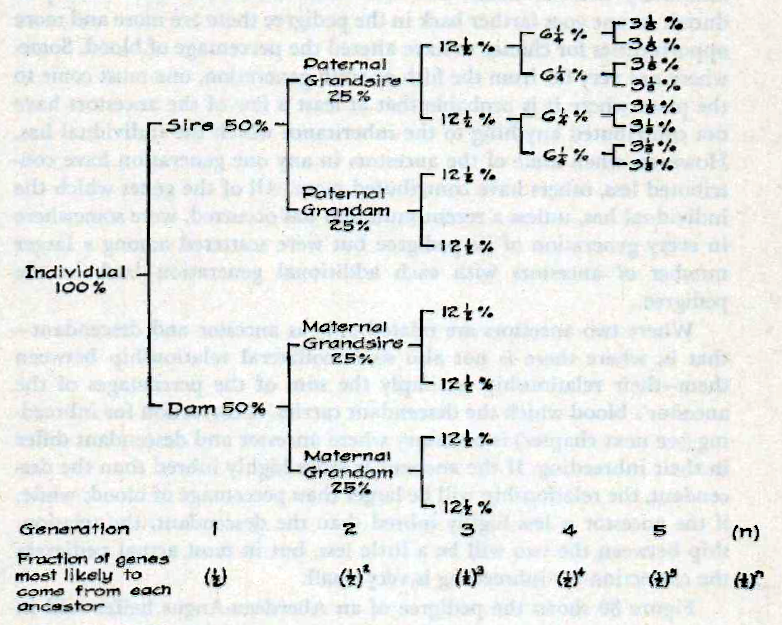
\includegraphics[width=\textwidth]{Figure_29.png}
    \caption{The fraction of an individual's genes most likely to come from each ancestor.}
    \label{fig:Lush_Figure_29}
\end{figure}

\index{Percentage of blood|(}
The most probable proportion of an individual's genes to come
from each of its ancestors is 50 per cent from a parent, 25 per cent from
a grandparent, 12\nicefrac{1}{2} per cent from a great grandparent, and so on, the
percentage being halved with each additional generation the ancestor
is farther back in the pedigree. Because of the part chance plays in
Mendelian inheritance, these percentages need not be exact for an
ancestor farther back than a parent. So far as concerns any one great,
great, great grandparent, the most probable expectation is that the individual
will have inherited \nicefrac{1}{32} of all its genes from that ancestor. Even
in animals having 30 pairs of \index{Chromosomes}chromosomes, this does not average quite
two chromosomes from each ancestor in that generation. Since there is
some crossing-over, it is probable that the individual will still have at
least a few genes from every ancestor in that generation. However, it
could happen that certain ancestors in that generation would have contributed
nothing at all to this individual's inheritance. So far as concerns
the inheritance which the descendant has, such ancestors might as
well never have existed except that they were a part of the living
machinery without which this individual would not have been produced.
As one goes farther back in the pedigree there are more and more
opportunities for chance to have altered the percentage of blood. Somewhere
not very far from the fifth or sixth generation, one must come to
the place where it is probable that at least a few of the ancestors have
not contributed anything to the inheritance which the individual has.
However, when some of the ancestors in any one generation have contributed
less, others have contributed more. All of the genes which the
individual has, unless a recent mutation has occurred, were somewhere
in every generation of its pedigree but were scattered among a larger
number of ancestors with each additional generation back in the
pedigree.

Where two ancestors are related only as ancestor and descendant that
is, where there is not also some collateral relationship between
them -- their relationship is simply the sum of the percentages of the
ancestor's blood which the descendant carries. A correction for inbreeding
(see next chapter) is necessary where ancestor and descendant differ
in their inbreeding. If the ancestor is more highly inbred than the descendant,
the relationship will be larger than percentage of blood; while,
if the ancestor is less highly inbred than the descendant, the relationship
between the two will be a little less, but in most actual pedigrees
the correction for inbreeding is very small.

Figure~\ref{fig:Lush_Figure_30} shows the pedigree of an Aberdeen-Angus heifer sold in
1931 in the Strathmore sale. This heifer ``carries 81\nicefrac{1}{4} per cent of the
blood of'' Earl Marshall. This figure is the sum of: 25 per cent for each
of Earl Marshall's two appearances as grandsire, 12\nicefrac{1}{2} per cent for each
of his two appearances as great grandsire, and 6\nicefrac{1}{4} per cent for his one
appearance as great great grandsire in this pedigree. By similar computations
it will be seen that Earl Marshall 50th carries 87\nicefrac{1}{2} per cent of
the blood of Earl Marshall and that Blackcap Empress 74th carries 75
per cent of the blood of Earl Marshall. The percentage of Earl Marshall
blood in the daughter is naturally the average of that in her parents.
These figures for percentage of blood need only a small correction for
inbreeding (larger than usual in this case) to become the coefficients of
relationship of Earl Marshall to these three descendants of his.

\index{Collateral relatives|(}Collateral relationship between two animals is computed separately
for each line of descent by which it is possible to go from one of them
back to the common ancestor and then down to the other. Each generation
in this line of descent is another Mendelian segregation halving the
fraction of genes which are likely to be duplicates in the two animals
because of their common descent. If there are many more than four or
five intervening segregations, the amount of relationship through any
one such line will be insignificantly small; but if there are many such
lines, their total may be large enough to be of some importance.
\noclub[2]

\begin{figure}
	\centering
    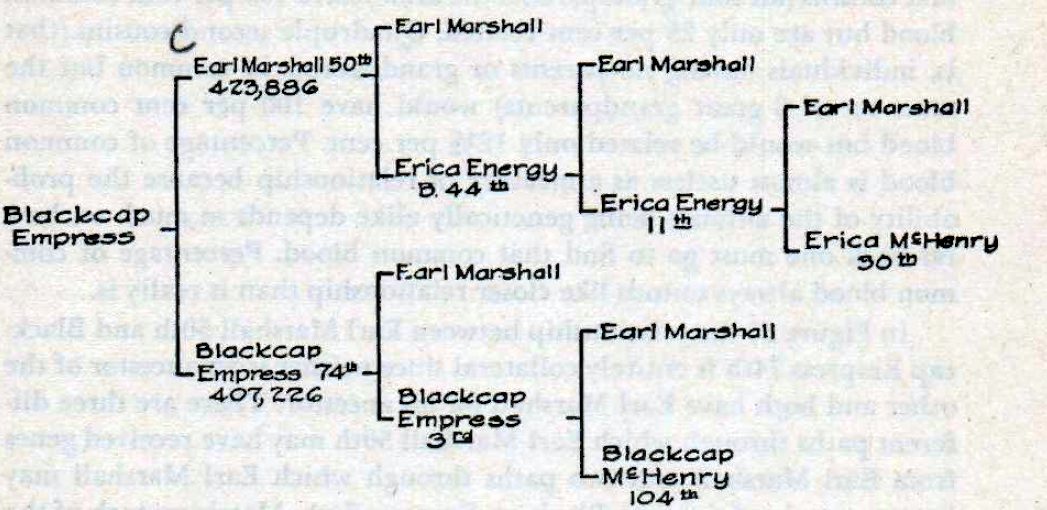
\includegraphics[width=\textwidth]{Figure_30.png}
    \caption{A pedigree showing high relationship to the Aberdeen-Angus bull, Earl
			 Marshall.}
    \label{fig:Lush_Figure_30}
\end{figure}

The probability that cousins will have the same genes may be computed
by extending the same process used for computing the relationship
between half brothers. For each pair of genes the chance is one-half
that a grandparent will give the same gene to both its offspring. Only
one-half the times when this does happen will this same gene be transmitted
to the one cousin. In only one-half of those cases will the other
offspring transmit the same gene to the other cousin. There is, therefore,
one chance in eight that an identical gene shall reach two cousins
from a common grandparent. Even this concerns only half of their
inheritance, since the other half comes from their other parent. Hence
the probable genetic likeness between cousins on account of common
descent from one grandparent is that \nicefrac{1}{16} of their genes will be identical
because of this. If, as is usually the case with human first cousins,
they have two grandparents in common, this adds an equal probability
of their having the same genes through descent from that other grandparent.
This makes a total probability that \nicefrac{1}{8} of their genes will be
alike because of the common ancestry, while the rest of their genes are
no more and no less apt to be alike than if they were unrelated members
of the same freely interbreeding population.

Breeders sometimes measure collateral relationship by ``percentage
of common blood,'' but this can be very misleading. Full brothers have
100 per cent common blood but are only 50 per cent related; double
first cousins (all four grandparents the same) have 100 per cent common
blood but are only 25 per cent related. Quadruple second cousins (that
is, individuals having no parents or grandparents in common but the
same set of 8 great grandparents) would have 100 per cent common
blood but would be related only 12\nicefrac{1}{2} per cent. Percentage of common
blood is almost useless as a measure of relationship because the probability
of the animals being genetically alike depends so much on how
far back one must go to find that common blood. Percentage of common
blood always sounds like closer relationship than it really is.

In Figure~\ref{fig:Lush_Figure_30} the relationship between Earl Marshall 50th and Blackcap
Empress 74th is entirely collateral since neither is an ancestor of the
other and both have Earl Marshall for an ancestor. There are three different
paths through which Earl Marshall 50th may have received genes
from Earl Marshall and two paths through which Earl Marshall may
have transmitted genes to Blackcap Empress 74th. Matching each of the
three ways with each of the two ways makes six different ways in which
these two descendants of Earl Marshall might have received duplicates
of any gene which was in him. The fact that Earl Marshall is the
sire of both contributes 25 per cent to their relationship. The two different
ways in which he is the sire of one and the grandsire of the other
contribute 12\nicefrac{1}{2} per cent each. Descent from him as grandsire on both
sides contributes 6\nicefrac{1}{4} per cent. Descent from him as sire of one and great
grandsire of the other contributes another 6\nicefrac{1}{4} per cent. Finally the
small probability that these two animals would get identical genes by
the long route from Earl Marshall as great grandsire of one and grandsire
of the other contributes another 3\nicefrac{1}{8}  per cent to their relationship.
This makes a total of 65\nicefrac{51}{8} per cent, all of it coming through their descent
from Earl Marshall, but that is still to be corrected for their
inbreeding. A somewhat simpler way of figuring their relationship in
this case, where they have only one ancestor in common, is to find that
one of them has 75 per cent of the blood of Earl Marshall, while the
other has 87\nicefrac{1}{2} per cent, and to \textit{multiply} those two percentages together.
This method gives the same answer; but if the two animals had more
than one ancestor in common, the computations would have to be made
separately for each such ancestor. This method will lead to difficulties
if the common ancestors are related to each other.

These rules for computing relationships are nothing but counting
the number of Mendelian segregations which have intervened in each
line of descent connecting two individuals, and using $(1/2)^n$ aas the fraction
of their genes which are likely to be identical because the two animals
received duplicate genes in that way from their common ancestor.

When one animal is an ancestor of the other and they are also
related collaterally because both are descended from a third animal, it
is usually more convenient to compute the direct relationship first. An
example of this can be had from Figure~\ref{fig:Lush_Figure_30} if we wish to learn how closely
Earl Marshall 50th is related to his daughter, Blackcap Empress.
They are directly related as sire and daughter, and in addition he may
have received from Earl Marshall some genes for which she received
duplicates through her dam. He traces to Earl Marshall in three different
lines, the number of generations in each being 1, 2, 3, respectively,
while she traces through her dam to Earl Marshall in two lines, the
number of generations being 2 and 3 in those. Combination of each of
the two with each of the three makes six different ways in which these
two animals may have received duplicate genes by descent from Earl
Marshall. The sum of the separate values for these six paths equals
32 \nicefrac{13}{16} per cent collateral relationship to be added to the 50 per cent
direct relationship. That total is still to be corrected for the inbreeding,
which in this case is intense enough to make that correction rather
large.

Figure~\ref{fig:Lush_Figure_31} shows another example. The relationship of X to A is
both direct and collateral, while the relationship between X and Z is
entirely collateral, neither being an ancestor of the other. The arrow
diagram of the pedigree is often very convenient for showing at a glance
the nature of the relationship. If the pedigrees are complicated by much
inbreeding, the arrow diagram is almost necessary in order not to omit
some lines of relationship nor count some a second time without being
aware of having done so. The relationship of X to Z in Figure~\ref{fig:Lush_Figure_31} will
illustrate why percentage of common blood is not dependable as a
measure of collateral relationship. It is not legitimate to say that 75 per
cent of X's blood is the same as 100 per cent of Z's blood and to estimate
their relationship through manipulating these figures of ``common
blood'' in any way. It is legitimate to do this separately for each common
ancestor and to say that Z has 50 per cent of the blood of D and X
has 25 per cent of that blood and that Z and X are therefore related 50
per cent of 25 per cent, or 12½ per cent, through D. Also, it is legitimate
to say that both Z and X have 50 per cent of the blood of C and
that 50 per cent of 50 per cent equals 25 per cent of relationship
between Z and X through descent from C. This 25 per cent may then
be added to the 12\nicefrac{1}{2} per cent of relationship through D to give the total
relationship of 37\nicefrac{1}{2} per cent.
\index{Collateral relatives|)}
\index{Percentage of blood|)}

Relationship between two individuals cannot be higher than 50 per
cent unless some inbreeding has been practiced. The only exception to
this concerns identical twins, and members of the same ``clone'' in
plants and animals which can be propagated asexually. Relationship
between members of such isogenic lines is 100 per cent, since they are
really duplicates of the same zygote and there has been no intervening
Mendelian segregation or recombination to permit them to have unlike
genes. Since not much inbreeding occurs in most animal species or in
man, we rarely have a chance to see the resemblance between animals
related much more closely than 50 per cent. It is largely for this reason
that identical twins\index{Identical twins} are such interesting evidence about the importance
of heredity. An increase from 50 to 100 per cent in genetic likeness
makes a marked difference in the variation to be expected between individuals,
especially in characteristics which are highly hereditary.

\begin{figure}
	\centering
    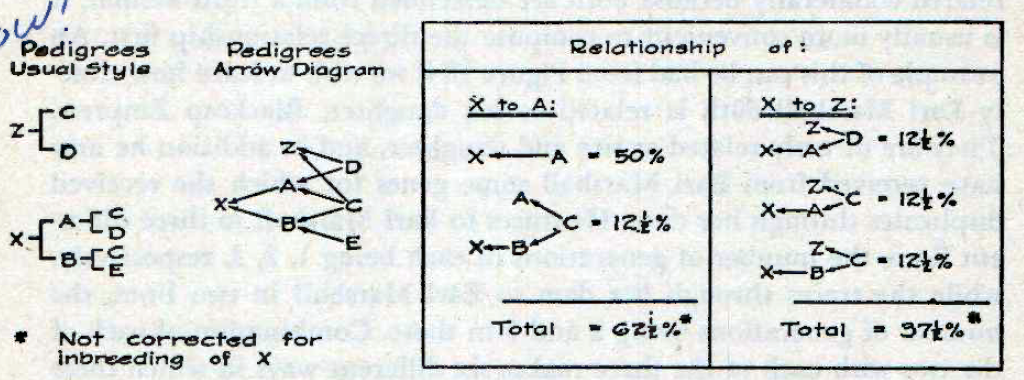
\includegraphics[width=\textwidth]{Figure_31.png}
    \caption{Showing how relationship is computed.}
    \label{fig:Lush_Figure_31}
\end{figure}

Two animals cannot be very closely related if all their common
ancestors are distant ones. Rarely is much gained by going back farther
than three or four generations in the pedigrees of two animals to see
whether they are related. In an extreme case two animals might have
the very same 16 great great grandparents, and yet their relationship to
each other would be only 6\nicefrac{1}{4} per cent if they had no parents, grandparents,
or great grandparents in common and if there were no inbreeding
involved.

Relationship is sometimes measured in ``degrees,'' especially for
legal purposes. In civil law a degree of relationship corresponds to a
generation of Mendelian segregation. Thus parent and offspring are
``related in the first degree,'' grandparent and offspring are ``related in
the second degree,'' uncle and nephew are ``related in the third degree,''
etc. When the individuals are related through more than one line of
descent, each line is computed and stated separately without combination
into a single figure. In canon law and common law only the number
of generations in the longer line of descent from the common
ancestor is counted. Thus uncle and nephew are related in the second
degree by canon law and common law.

\section*{THE EFFECTS OF SEX-LINKAGE}
\label{page255}
\index{Sex linkage}

In the mammals the male is the heterogametic sex. His sex-linked
inheritance comes entirely from his mother. Her sex-linked inheritance
is present in duplicate, and among the pairs of sex-linked genes which
are heterozygous in her, chance at segregation determines what sex-linked
inheritance a son shall receive. The result is that 100 per cent of
his sex-linked genes are like 50 per cent of hers. The square root of the
product of these is the relationship (71 per cent) of son and dam for sexlinked
genes. The sex-linked inheritance of a female comes equally
from both parents; but since her sire does not have a duplicate set of
sex-linked genes, chance plays no part in determining what sex-linked
inheritance she shall receive from him. So far as his daughters are concerned,
the situation is the same as if the sire were homozygous for all
his sex-linked genes. The relationship between sire and daughter is also
71 per cent for sex-linked genes, since 100 per cent of those in the sire
are like 50 per cent of those in his daughter. Daughter and dam are
related 50 per cent for sex-linked genes, just as they are for autosomal
genes. Sire and son are not related at all for sex-linked genes, since the
son cannot receive any of those from his sire. The practical consequence
of sex-linkage is to make the parent-offspring relationship higher
between opposite sexes than it is between parent and offspring of the
same sex. In birds, moths, and some fishes the female is heterogametic,
but that leaves the practical situation nearly the same: namely, that
males are a bit more closely related to their dams and females to their
sires than either is to the parent which is the same sex. The lowest relationship
for sex-linked genes is that between sire and son in the mammals,
but between dam and daughter in birds.

This difference in relationship to ancestors of different sexes is
partially, but not entirely, equalized as one goes further back in the
pedigree , since a dam may transmit either the sex-linked genes she got
from her sire or the sex-linked genes she got from her dam.

Since the farm animals have about 20 to 30 pairs of \index{Chromosomes}chromosomes
and only one pair carries the sex-linked genes, it is improbable that the
total amount of sex-linked inheritance is much larger than 3 to 5 per
cent of the total inheritance. Hence, for practical purposes no material
error is introduced by neglecting sex-linkage when computing relationships.
(See table \ref{tbl:Lush_Table_20}.) Occasionally there may be individual matings in
which sex-linkage will play a noticeable part.
\index{Relationship!measurement of|)}

\section*{PRACTICAL USES OF THE RELATIONSHIP COEFFICIENT}
\index{Ancestors, importance of various ones|(}
\index{Pedigrees as aids to selection|(}

The most important practical use of the relationship coefficient is to
predict the merit of relatives of animals whose merit is known. This is
the whole basis for using the merit of relatives to aid in making selection
more effective. If nothing at all is known about an animal or its
relatives, the only prediction we can make is that it will be an average
animal of its breed. Neglecting for the moment the effects of environment,
dominance, epistasis, and selection, if we know an animal related
40 per cent to the unknown one, the most probable prediction is that
the unknown animal will deviate from the breed average in the same
direction as the known relative does, but only 40 per cent as far. If a
cow's genotype for fat production is 100 pounds above the breed average
the most probable genotype of her daughter, if nothing is known
about the sire except that he belonged to the same breed, is that the
daughter's genotype will be 50 pounds above the breed average.
Numerous practical difficulties and necessary precautions beset this use
of relationship as a measure of how much weight to put on each relative
in estimating the breeding worth of an animal. Most of those hinge
around the inescapable fact that we are not sure of the genotypes of the
relatives but only know their apparent merit. The two may be widely
different if outward merit is much affected by environment, dominance,
or epistasis. Other difficulties concern the weight to give each relative in
combining information about several related ones, not all known equally
well, into the best single estimate of what the unknown animal will
be. The practical aspects of this were discussed in chapter \ref{cha:Lush_Chapter_14}. They put
serious limitations on the practical usefulness of the principle-which is
true when comparing equally well-known relatives of which one is to
be used alone in such estimates-that the attention to be given such
relatives is in proportion to their relationship to the animal to be estimated.
The relationship between an individual and the average genotype
of a group of its relatives may be higher than its relationship to
any one of them. The simplest and most important example of this is
the case of half sibs. In the extreme case of a characteristic perfectly
hereditary in the simple additive way, and unselected half sibs from a
random breeding population, the equation for predicting with the
least error what an individual will be from knowing \textit{p} of its paternal
half sibs and \textit{m} of its maternal half sibs is:

{\setlength{\tabcolsep}{0.1em} % for the horizontal padding}
\begin{table}[h]
	\centering
	\begin{tabular}{lll}
		Animal $=$ breed average & \(+ \dfrac{p}{p + 3}\) & (paternal half sibs minus breed\\
			   					 & 						  & average)\\
			   					 & \(+ \dfrac{m}{m + 3}\) & (maternal half sibs minus breed\\
			   					 & 						  & average)\\
	\end{tabular}
\end{table}

\noindent
As \textit{p} and \textit{m} increase from one to at least four or five, the usefulness of
this equation goes up rapidly and it soon comes close to the limit set by
perfect knowledge of the genotypes of sire and dam of the individual
being predicted. Of course, in actual practice there are effects of environment
and dominance and \index{Epistatic effects}epistasis and possible previous selection of
half sibs which will usually make it wise to put less weight than this on
what the half sibs indicate. The above equation shows quantitatively
what we are recommending if we advise choosing a son of a proved sire
and a proved dam.

To the extent that the trait being measured is affected by environment,
dominance, and epistasis, actually observed likeness will be less
than the genetic likeness unless each pair of related individuals tended
to be exposed to an environment alike for them but different from the
environment of other pairs. In that case the observed may be higher
than the calculated. Thus, in a random bred population hal£ sisters are
genetically as much alike as grandam and granddaughter; but each pair
of half sisters is more apt to have been exposed to the same more or less
unusual environment than is each grandam and granddaughter pair.
Hence, in such data as official dairy records, it is to be expected that the
observed likeness between half sisters will be larger than that between
grandam and granddaughter. For the same reason paternal half sisters,
which are usually contemporaries, may be expected actually to resemble
each other a little more closely than maternal half sisters. The latter
may have been born and reared several years apart.

\index{Dominance}Dominance and epistasis make observed likenesses generally lower
than calculated ones, but in certain relationships-of which the most
important is that between full sibs-dominance produces a little extra
likeness on its own account. This partly offsets its general tendency to
lower likenesses.

If breeders' ideals diverge enough that they have been selecting for
distinctly different types within the same breed, then animals in the
same herd are apt to resemble each other, relative to the whole breed,
more than their relationships indicate.
\index{Ancestors, importance of various ones|)}
\index{Pedigrees as aids to selection|)}
\noclub[3]

\section*{GALTON'S LAW}
\index{Galton's ``Law''|(}

Two distinct although related ideas are sometimes confused under
the name ``Gallon's Law.'' The first is the observed fact that the correlation
between parent and offspring is nearly $+ .50$ in populations
where there is not much inbreeding and where the trait being measured
is highly hereditary. The correlation between an animal and a more
remote ancestor is halved for each additional generation which separates
them. This is precisely what was shown in Figure~\ref{fig:Lush_Figure_29} and was
discussed under ``percentage of blood.''\index{Percentage of blood} It was an observed fact in Galton's
time and had been used by practical breeders in England from at least
as long ago as 1815.\footnote{According to the encyclopedia of J. G. Krtinitz}
The only material difference now is that we understand
why it is a natural consequence of the laws of inheritance, provided
the population is mating at random and the trait being studied is
entirely hereditary in the simple additive manner. Naturally the extent
to which these conditions are fulfilled varies in different populations
and even for different traits in the same population and often is known
only within rather wide limits.

\begin{figure}[!htbp]
	\centering
    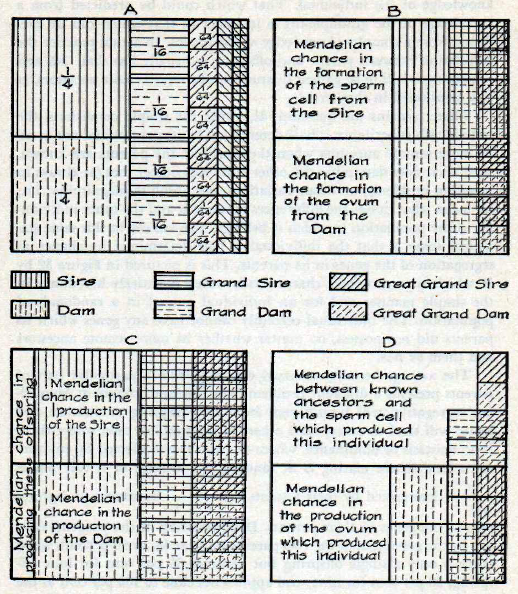
\includegraphics[width=.9\textwidth]{Figure_32.png}
    \caption{Galton's ``law'' of the relative importance of various ancestors, pictured
			 for a characteristic perfectly hereditary in the simple additive way. A: As formulated
			 by Galton, each ancestor being considered singly. B: Correctly pictured for an individual
			 animal in a random breeding population. That which can be predicted from
			 the more remote ancestors is included in what can be predicted from the intervening
			 ancestors. Mendelian chance at segregation accounts for half of the determination in
			 the statistical sense of that word. C: Same as B except that this concerns the average
			 inheritance of nine unselected offspring from one pair of parents. The effects of
			 chance in the nine segregations which produced the sperm cells and in the nine 
			 segregations which produced the ova tend Lo cancel each other to such an extent that
			 Mendelian chance now determines only one-tenth of the average inheritance of these
			 nine instead of the one-half which it determines for each individual. D: Determination
			 of the individual by known characteristics of its ancestors in the case where
			 males cannot express the characteristic themselves and neither the sire nor the two
			 grandsires were progeny-tested.}
    \label{fig:Lush_Figure_32}
\end{figure}

The other part of Galton's law --- which unfortunately is the part
most frequently quoted --- is true only in a specialized statistical sense.
The square of the correlation coefficient measures the portion of the
variance in one variable which disappears in data in which the other
variable is constant. In this special statistical sense the individual's
inheritance is \nicefrac{1}{4} determined by its sire and¼ by its dam. That instantly
raises the question: What determines the remaining \nicefrac{1}{2}? Galton reasoned
that this same process would be repeated with the sire and with
the dam, each of them being \nicefrac{1}{4} determined by its sire and another \nicefrac{1}{4}
by its dam, and that if this process were pursued far enough the fractions
would ultimately add up to one. Consequently he proposed as a
general ``law'' that the individual's inheritance was \nicefrac{1}{4} determined by
its sire and \nicefrac{1}{4} by its dam, \nicefrac{1}{16} by each of the
four grandparents, \nicefrac{1}{64} by each of the 8 great grandparents, and
so on, each ancestor contributing just \nicefrac{1}{4} as much to the total
inheritance as did the one a generation nearer to the individual. This is
usually pictured as in A, of Figure~\ref{fig:Lush_Figure_32}. Because this
seemed a logical scheme, it was accepted rather widely
and even today is sometimes quoted with approval. Unfortunately, the
obvious inference from this diagram (that if one knew all about all of
the ancestors, he would know all about the heredity of this individual)
is not true.

\begin{figure}[!htbp]
	\centering
    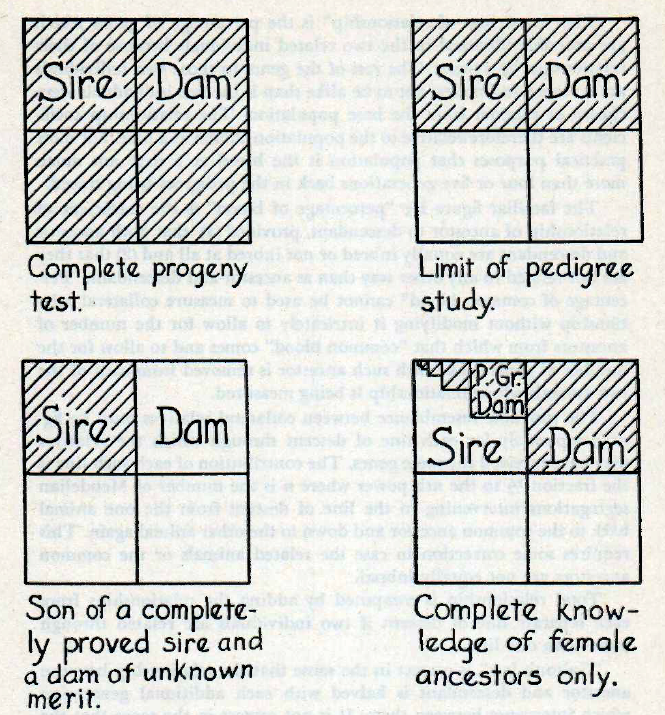
\includegraphics[width=.9\textwidth]{Figure_33.png}
    \caption{Relative accuracy of a progeny test and of various kinds of pedigrees
			 when the information in each is as complete as is theoretically possible under the
			 conditions named. Shaded areas represent portions of the individual's inheritance
			 determined (in the statistical sense) by complete information of the kind pictured.
			 The correlation between the acmal and the predicted breeding value of the indi vidual
			 would be the square root of the shaded fraction of the area; i.e., 1.0 in the
			 upper lefthand corner, .71 in the upper right, .50 in the lower left, and .58 in the
			 lower right. The unshaded areas represent possibilities for Mendelian segregation to
			 have made the individual's actual breeding value higher or lower than its expected
			 breeding value.}
    \label{fig:Lush_Figure_33}
\end{figure}

Had Galton used multiple correlation technique (as Yule pointed
out at the third International Genetics Congress in 1906) he would
have found that the partial correlation between grandparent and
grandson or granddaughter, the intervening parent being held constant,
is zero in any population in which the correlation between parent
and offspring is .50 and the correlation between grandparent and
grandson or granddaughter is .25. If the parent's heredity is not known,
it is still true in the technical statistical sense of the word that the individual
is ``determined'' \nicefrac{1}{16} by each of its grandparents. That is shown
for the paternal grandam by D in Figure~\ref{fig:Lush_Figure_32}. But if the parent's heredity
is known, knowledge of the grandparents adds nothing to the
knowledge of the individual. That which could be predicted from a
knowledge of the grandparent is included in that which can be pre- ·
dieted from a complete knowledge of the parent. In actual practice the
correlation between parent and offspring is usually less than .50, and
something is still to be gained by studying the more remote ancestors, as
was mentioned in chapter~\ref{cha:Lush_Chapter_14}.

There remains the question: If, under the simple conditions, the
individual's inheritance is half determined by its parents and not at all
by more remote ancestors when the merits of the parents are known,
then what does determine the other half? Remember that (as always in
breeding problems) we mean variations, not absolute magnitudes; i.e.,
we mean what causes the differences between it and the other individuals
in the population to which it belongs. The answer in this same statistical
sense is that the individual is half determined by chance at
segregation of the genes in its parents. This is pictured in
Figure~\ref{fig:Lush_Figure_32} by B, which is correct for a characteristic
which is entirely hereditary in the simple manner and for an individual
animal in a random-bred population. The individual certainly cannot have
any genes which its parents did not possess, no matter whether its more
remote ancestors had them or not.

\index{Progeny test|(}
The average heredity of many offspring from a particular pair of
parents presents a different problem. The results of chance at Mendelian
segregation will be different from one offspring to another and
hence will tend to cancel each other. In the simplest case, where there
is no epistasis or dominance, where the trait is not affected by environment,
and where mating is at random, the average of \textit{n} full sibs is
$\dfrac{n}{n + 1}$ determined by their parents and $\dfrac{1}{n + 1}$ by chance at
segregation of the genes in their parents. Determination of the progeny average
by the genotypes of the two parents starts at \nicefrac{1}{2}, or 50 percent, when
there is only a single offspring but becomes 80 per cent for four offspring,
90 per cent for nine, and approaches close to 100 per cent as the
numbers of offspring become very large. This is pictured in C of
Figure~\ref{fig:Lush_Figure_32} for the case where \textit{n} = 9. This is why complete knowledge of 
the genotypes of the parents would permit predicting with almost perfect
accuracy what the average of their progeny (if numerous) will be, even
though it would not permit highly accurate prediction of what each
individual offspring will be. D of Figure~\ref{fig:Lush_Figure_32} shows Galton's law when
the merits of some of the near ancestors on one side of the pedigree are
not known.
\index{Galton's ``Law''|)}
\index{Progeny test|)}

\section*{SUMMARY}

The genetic resemblance between individuals is based on the probability
that they have received identical genes from animals which are
ancestors of them both.

The ``coefficient of relationship''	 is the percentage of genes which
are probably identical in the two related individuals because of their
relationship by descent. The rest of the genes in those two individuals
are no more and no less apt to be alike than if the two individuals were
chosen at random from the base population. The relationship coefficients
are therefore relative to the population chosen as a base. For most
practical purposes that population is the breed at a date not much
more than four or five generations back in the pedigrees being traced.

The familiar figure for ``percentage of blood''\index{Percentage of blood} is the coefficient of
relationship of ancestor to descendant, provided (l) that both ancestor
and descendant are equally inbred or not inbred at all and (2) that they
are not related in any other way than as ancestor and descendant. ``Percentage
of common blood'' cannot be used to measure collateral relationship
without modifying it intricately to allow for the number of
ancestors from which that ``common blood'' comes and to allow for the
number of generations each such ancestor is removed from each of the
two animals whose relationship is being measured.

The probable resemblance between collateral relatives must be figured
separately for each line of descent through which the relatives
may have received the same genes. The contribution of each such line is
the fraction \nicefrac{1}{2} to the \textit{n}th power where \textit{n}
is the number of Mendelian segregations intervening in the line of descent
from the one animal back to the common ancestor and down to the other
animal again. This requires some correction in case the related animals
or the common ancestors are not equally inbred.

Total relationship is computed by adding the relationships from
each separate line of descent if two individuals are related through
more than one line.

``Gallon's law'' is correct in the sense that the relationship between
ancestor and descendant is halved with each additional generation
which intervenes between them. It is not correct in the sense that the
individual's heredity is completely determined by the heredity of its
ancestors. In that sense in a random-bred population the individual is
one-fourth determined by each parent and one-half determined by
chance in Mendelian segregation. Determination by more remote ancestors
is included in the determination by the parent.

The existence of sex-linkage causes sons to resemble dams a little
more than they do their sires and makes daughters resemble their sires
a bit more closely than they do their dams. This effect must be small in
most cases.

Relationship measures the probability that individuals will be alike
\textit{in their genes}. Their actual outward likeness depends also upon how
much the traits being measured are affected by environment, dominance,
and epistasis, upon the extent to which their environments were
correlated, and upon whether their ancestors were mated like to like.

The most important practical use for relationships is in predicting
the most probable merit of unknown or perhaps even unborn individuals
from the merit of their known relatives.

\section*{REFERENCES}

\begin{hangparas}{0.5in}{1}%
Davenport, E. D. 1907. Principles of breeding, pp. 525--34.

Fairchild, David . 1921. A genetic portrait chart. Jour. of Heredity, 12:213--19.

Wright, Sewall. 1922. Coefficients of inbreeding and relationship. Amer. Nat., 56:330--38.

---. 1923. Mendelian analysis of the pure breeds of livestock. I. The measurement
of inbreeding and relationship. Jour. of Heredity, 14:339--48.
\end{hangparas}
\index{Relationship|)}
\chapter{The Consequences and Measurement of Inbreeding}
\label{cha:Lush_Chapter_21}
\index{Inbreeding|(}

Inbreeding is the mating of closely related animals. Everyone agrees
to that general definition, but there is much diversity of usage about
how closely related the mates must be before the mating should be
called inbreeding. Many practical breeders restrict the word inbreeding
to the mating of full brother and sister or of parent and offspring. Others
would call the mating of half brother and sister, or the mating of
grandparent to grandson or granddaughter inbreeding. The broad
scientific definition is that inbreeding is the mating of animals more
closely related to each other than the average relationship within the
population concerned. Such matings tend to make the offspring more
homozygous than if their parents were of average relationship to each
other. Mating of animals less closely related than the average of the
population concerned is outbreeding.

The population concerned would usually be the whole breed when
this definition is applied to animal breeding, but might be the race or
the whole species when considering the part which inbreeding may
play in evolution. The intensity of the inbreeding is very slight, however,
unless the mates are quite closely related or the inbreeding is continued
for many generations. This leads to the convenient situation
that the great majority of all breedings which take place within a pure
breed are practically neutral so far as any inbreeding or outbreeding
effect is concerned and may be classed as random breeding, even though
one does not know the average relationship within the breed. The practical
use of the definition that inbreeding is the mating of closely related
animals merely requires agreement as to how close that relationship
must be.

It is impossible to define inbreeding simply as the mating of related
animals. All animals that can be mated at all are related, at least slightly.
Each individual has two parents, four grandparents, eight great
grandparents, and so on, the number of ancestors doubling each generation.
In the tenth generation of its pedigree an animal will have more
than a thousand ancestors if there has been no inbreeding. If two ani-
thousand ancestors of the one cannot include any of the nearly contemporary
thousand ancestors of the other. If there has been no inbreeding,
each animal has more than a million ancestors in the twentieth generation
of its pedigree. If the pedigree is followed much further, these
numbers become greater than the number of animals alive at that time
could have been. For example, in man there are about three generations
to the century. The number of ancestors each person had living at the
time of William the Conqueror would be about $2{26}$, or roughly a little
more than 67 millions, if there had been no mating of relatives . Now
there never were that many people in Great Britain at any one time.
Anyone descended entirely from British ancestors must have had an
enormous amount of repetition of ancestors that far back in his pedigree,
especially since many individuals living at any one time leave no
descendants. One whose ancestors came from several nations has only
to follow his pedigree a few centuries further back (no further than to
900 A.D. at the outside) to find that, if there had been no mating of relatives,
he would have had more ancestors alive at that time than there
were people on earth!

This situation is more extreme in livestock breeding. The Brown
Swiss breed in the United States is descended entirely from 129 cows
and 21 bulls which were imported into this country. In American Rambouillet
pedigrees about 45 per cent of the lines traced back at random
end in sheep from the von Homeyer flock in Germany. Over half of
the random pedigree lines of the Shorthorn breed go to one bull,
Favourite. Similar things are true of other breeds, although few breeds
are yet explored in detail from this point of view. Moreover, this
includes only what has happened since pedigree recording began. That
is a comparatively short time --- about 150 years in the Shorthorns and
only about 50 years in the other two breeds mentioned.

The definition of inbreeding must be relative to some group or
population. Pure breeding, for instance, is inbreeding relative to the
whole species but need not be and rarely is inbreeding of noticeable
intensity relative to the breed. Figure~\ref{fig:Lush_Figure_34} illustrates
the situation diagrammatically from closest inbreeding to widest outbreeding. To the
left of random mating are the inbreeding matings while the outbreed ing
ones are to the right. The closeness of the two lines to each other in
Figure 34 represents how closely the mates are related to each other.
That ranges from complete identity in the case of self-fertilization (possible
in most plants but impossible in any farm animal) through close
relatives, members of the same breed, members of different breeds but
the same species, members of different species within the same genus,
and perhaps even members of different genera. The offspring of species
crosses usually exhibit some degree of sterility. Generic crosses are very
rare. Presumably the genotypes of the individuals are so unlike that
the union, even if possible at all, produces no living offspring.

\section*{THE CONSEQUENCES OF INBREEDING}
\index{Gene frequency|(}
\index{Heterozygosis|(}
\index{Homozygosis|(}

The primary effect of inbreeding is to increase the probability that
the offspring will inherit the same thing from sire and dam. This tends
to lower the percentage of heterozygosis in the population and to produce
relationships higher than 50 per cent. All the other effects of
inbreeding result from those. In each inbred line the genes which are to
be in the next generation are a sample of those which were in the preceding
generation. Because the sample is small the gene frequency in it
will often by chance differ considerably from the gene frequency in the
generation from which the sample came. Thus the gene frequency can
wander back and forth until it reaches either zero or one. Then the line
is homozygous for that particular gene or its allel. This homozygosis
cannot be lost, except by mutation, as long as the inbreeding is continued.
The genes which are heterozygous are still subject to the
possibility of becoming homozygous each generation the inbreeding
continues. The fewer animals there are in the inbred line the smaller
is the sample of gametes which are needed to constitute the next generation
and the farther the frequency of each gene can drift up or down
in any one generation.

\begin{figure}
	\centering
    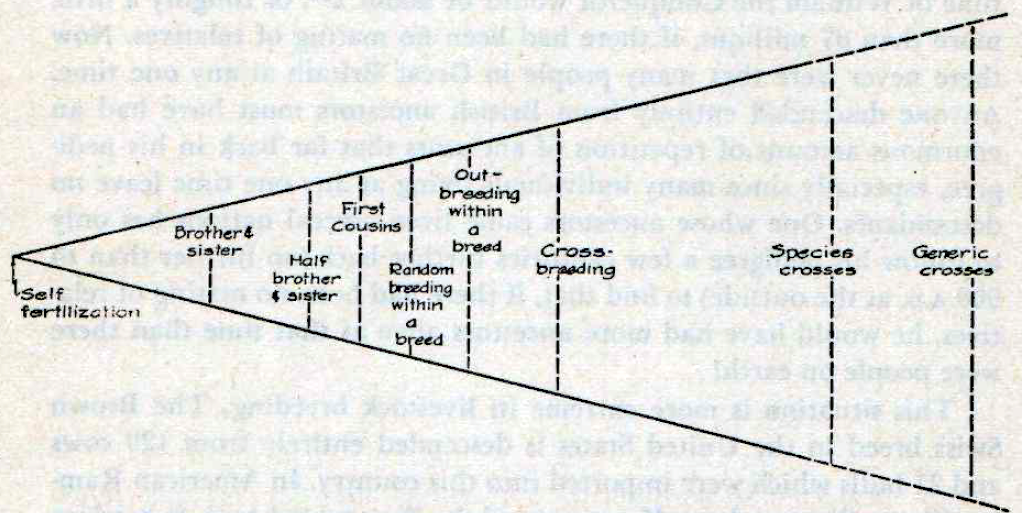
\includegraphics[width=\textwidth]{Figure_34.png}
    \caption{Degrees of inbreeding arranged according to the relationship between mates.}
    \label{fig:Lush_Figure_34}
\end{figure}

Because this change in gene frequency is random (equally likely to
be up or down), inbreeding is in conflict with selection whenever selection
is tending to keep a gene at some equilibrium frequency, as when
the heterozygote\index{Selection!for heterozygotes|(} is preferred. Inbreeding is continually causing the
gene `frequency to drift away from that equilibrium point in either
direction and selection is continually tending to take it back there.
When the inbreeding is very mild and selection is intense, the gene frequency
cannot get far from its equilibrium value. But when the
inbreeding is intense it may overwhelm selection and carry gene frequencies
far away from their equilibrium values, some above and some
below.

If the inbreeding is intense and continues long enough, and if there
are no mutations, the ultimate condition approached in each inbred
line is complete homozygosis in all pairs of genes. In some pairs it will
be the less desirable and in other pairs the more desirable gene which
becomes homozygous. Each inbred line is likely to differ from every other
inbred line in regard to which particular combination of genes
becomes homozygous in it, if many different pairs of genes are involved.
Inbreeding in animals almost never comes close to complete homozygosis
in actual practice. Even self-fertilized plants reach an equilibrium
point where the further loss of the remaining small amount of heterozygosis
just equals the new heterozygosis which mutations produce in
each generation. Mutations\index{Mutations} are so rare that for practical purposes they
can be neglected in considering inbreeding but they are mentioned
here for completeness.

The Mendelian basis of the inbreeding effect can be illustrated most
simply by the extreme case of self-fertilization. Each generation in each
inbred line consists of one individual in which, of course, each gene is
either homozygous or heterozygous. That is, gene frequency can have
only the values: .0, .5, or 1.0. Genes which are already homozygous in
the whole line must remain so as long as the inbreeding continues,
unless a mutation occurs. Pairs of genes which are heterozygous may be
considered as a population of the two kinds of genes in equal numbers,
from which two genes are to constitute the population in the next generation.
The probabilities that those two will be \textit{AA}, \textit{Aa}, or \textit{aa}, are in
the ratio 1 : 2 : 1. Thus half of all heterozygous genes in a self-fertilized
individual may be expected to become homozygous in its offspring.
Selection favoring either homozygote will tend to hasten the rate of
approach to homozygosis, while selection favoring the heterozygote will
tend to retard it. If there are many heterozygous pairs of genes, several
will become homozygous in every individual; and selection can have
only trivial effects in delaying any such rapid rate of approach toward
homozygosis. For example, if a self-fertilized individual is heterozygous
for 10 pairs of genes, only 1 offspring in 1,024 would be as heterozygous
as its parent. Even in species with reproductive rates which would permit
intense selection, it would be impossible to recognize genotypes
accurately enough to find such a rare heterozygous offspring every time
without mistake. If the inbreeding rate were lower or the number of
heterozygous genes were less, selection would have more chance to alter
the consequences of inbreeding. Actually, with each animal heterozygous
for scores of genes, many of which have only minor effects which
may be blurred by the effects of environment, the difference between
intense selection and no selection under self-fertilization has little more
effect on the outcome than the fate of a man dropped into the Niagara
River just a few yards above the falls would be affected by whether he is
a good swimmer or a poor swimmer! The difference in swimming ability
might be of tremendous importance if he were in comparatively
still water, as is roughly analogous to the situation in a population in
which the inbreeding is very mild, but would only rarely make a detectable
difference in the results in the presence of the much more powerful
force of the swiftly moving water.
\noclub[3]
\index{Selection!for heterozygotes|)}

Self-fertilization is impossible in the higher animals, but the Mendelian
basis of the inbreeding effect may be illustrated with the continued
inbreeding of full brother and sister. For each allelic set of genes
this constitutes a population of four genes-two in the sire and two in
the dam-from which four are to come to constitute the next generation.
Gene frequency can have only the values: .00, .25, .50, .75, or 1.00.
Although only one of them will occur in any one generation in any one
line, six different types of matings are possible. Those types are:

\begin{table}[h]
	\centering
	\begin{tabular}{C{3cm}C{3cm}C{3cm}}
						&						& Frequency of \textit{A} in \\
		Type 			& Mating				& this inbred line \\
		1				& \(AA \times AA\)		& 1.00 \\
		2				& \(AA \times Aa\)		& .75 \\
		3				& \(AA \times aa\)		& .50 \\
		4				& \(Aa \times Aa\)		& .50 \\
		5				& \(Aa \times aa\)		& .25 \\
		6				& \(aa \times aa\)		& .00 \\
	\end{tabular}
\end{table}

\noindent
If either the first or the last of these prevails, that line will remain
homozygous for that gene indefinitely, unless a mutation occurs. If
either the second or the fifth type prevails in one generation, there is
one chance in four that this line will become homozygous in the next
generation, two chances in four that it will remain the same, and one
chance in four that the next generation will be like the fourth type of
mating. When the line is of the third type, it will change to the fourth
type in the next generation. When it is of the fourth type, there is one
chance in eight that it will become homozygous in the next generation,
four chances in eight that it will change to types two or five, one chance
in eight that it will change to type three, and two chances in eight that
it will remain the same. Once the inbred line becomes type one or type
six, it remains that way. It can shift back and forth among the other
four types; but from them it will occasionally drift into types one or six,
from which it cannot return. Hence the ultimate end of all such lines
would be type one or type six if the inbreeding were continued long
enough. The drift from one type to another is so rapid in a population
as small as a line inbred full brother by sister that, after the inbreeding
gets well ·under way, nearly one-fifth of all the genes which are still heterozygous
in the line at any given time become homozygous in the next
generation. In larger populations the gene frequency would fluctuate
less extremely, but in any finite population it would do some shifting.
Inbreeding is only an extreme form of a process which exists to some
degree in all populations. The fact that the number of breeding individuals
in the poplation is finite permits gene frequency to vary
because of the sampling which takes place when the genes of one generation
are replaced by the genes of the next.

This Mendelian proof of the nature of the inbreeding process was
studied as long ago as 1914 by Fish, Jennings, and
Pearl,\footnote{\textit{Amer. Nat.}, 48:57--62, 491--94, 693--96, and 759--61.}
but it becomes extraordinarily difficult to follow even for regular
inbreeding systems milder than full brother by sister and practically
impossible to follow in the irregular inbreeding which occurs with farm
livestock. Wright in 1921 published a generalized explanation of the
consequences of milder forms of regular inbreeding and of irregular
inbreeding. In 1931 he generalized this still further to establish the
identity of the inbreeding effect and the general consequences of finite
population size, even in cases which we would not ordinarily call
inbreeding.\footnote{\textit{Genetics}, 6:124--43 and 16:106--29.}
\noclub

By changing heterozygotes to homozygotes, inbreeding brings to
light many of the recessive genes which would otherwise remain hid den.
Most recessive genes have less desirable effects than their alleles.
Inbreeding, therefore, usually lowers the average outward merit of the
inbred animals. Inbreeding permits more rapid improvement of the
breed by getting the recessive genes out from the shelter of their dominant
alleles so that they can be found more readily. For example, if 1
per cent of the calves in the Aberdeen-Angus breed are now born red
and the breeders were all to begin suddenly to inbreed as intensely as
mating parent and offspring or full brother and sister, the percentage of
red calves would in the first generation of inbred calves go up more
than threefold. The distribution of the genotypes\index{Zygotic ratios} before and after the
inbreeding would be as follows:

\begin{table}[h]
	\centering
	\begin{tabular}{L{6cm}L{2cm}L{2cm}L{2cm}}
		Before inbreeding:					& 81 \% \textit{BB}					& 18 \% \textit{Bb}	& 1    \% \textit{bb} \\
		After one generation of inbreeding:	& 83\nicefrac{1}{4}\% \textit{BB}	& 13 \nicefrac{1}{2}\% \textit{Bb}	& 3 \nicefrac{1}{4}\% \textit{bb}
	\end{tabular}
\end{table}

\noindent
The percentage of heterozygosis would decrease one-fourth, the genes
which would have been in heterozygous individuals now being equally
divided among the two kinds of homozygotes. The gene frequency has
not changed, but only the zygotic ratio. On account of dominance, the
desirable increase in \textit{BB} and decrease in \textit{Bb} individuals would not be
apparent outwardly. The only readily apparent change would be the
threefold increase in the proportion of red calves.
\index{Gene frequency|)}

For ages men have observed this general fact that inbreeding tends
to produce a certain amount of degeneration or decline in individual
merit. Formerly it was thought that the inbreeding in some mysterious
way actually damaged the inheritance and thus directly caused this
degeneration. Now it is understood that the inbreeding merely acts
somewhat as a detective does in uncovering crime -- not in creating it.
The undesired recessive genes are there all the time, but homozygous
recessive individuals appear more frequently when inbreeding begins.

More than any other breeding method, inbreeding tends quickly to
separate the population into many distinct families, each of which is
uniform within itself but distinct from others. This splitting of the
population into distinct families offers more opportunity for selection
between families than could take place in a random-bred population.
Inbreeding without selection leads toward a variable\index{Variation!increased by inbreeding} population composed
of unlike lines. If inbreeding were carried to completeness without
selection, the composition of the resulting population would be the
same as if the gametes from the initial population had suddenly been
transformed into zygotes by doubling all their chromosomes. If all the
genes acted only in an additive way, the genetic variance in the new
entirely homozygous population would be exactly twice what it was in
the original random-bred population, but would be entirely between
families, with no genetic variance within families. If many of the lines
were discarded, the population as a whole might then become more
uniform than it was before the inbreeding began; but that would be
primarily the result of discarding the poorer inbred lines rather than
a result of the inbreeding itself.

Inbreeding is especially powerful in forming \index{Family differences|(}families because the
genetic likeness of the mates does not depend upon the breeder's ability
to recognize which animals have similar genes when he mates them
together, as is the case with selection and with assortive mating. The
effects of inbreeding are not limited by the breeder's mistaking the
effects of environment, dominance, or \index{Epistatic effects}epistasis
for the effects of genes,
as the effects of those other breeding methods are. That is why inbreeding
is particularly powerful and useful in breeding for characteristics
which are only slightly hereditary. This difference also leads to the general
situation that under an inbreeding system the mates are more alike
in their heredity than they are in their appearance, whereas under
assortive mating they appear more like each other than they really are.
Where the correlation between genotype and phenotype is low, this
difference may be extreme.

Inbreeding may also produce some degeneration of individuals by
scattering the genes which in certain combinations produce a desirable
effect but which separately produce neutral or undesirable effects. If
there really is much of this epistasis, and if a breed has been under strict
selection for some time, there will have been a tendency to bring together,
in combinations where they will show good effects, those genes which
nick together well. Since most of those combinations will still be heterozygous,
at least for some of the genes concerned, any inbreeding will
tend to separate those combinations again and thus will lead to some
apparent loss of individual merit in addition to that coming entirely
from uncovering recessives.

Also inbreeding will lower the average merit of the population
directly by reducing heterozygosis among those pairs of genes in which
the heterozygote is more desirable than either homozygote.
\index{Family differences|)}

\section*{MEASURING THE INTENSITY OF INBREEDING}
\index{Inbreeding!measurement of|(}

Since the primary effect of inbreeding is to increase the probability
of receiving duplicate genes from sire and from dam, the measure of
inbreeding ought to be one which shows how much decrease in heterozygosis
is to be expected from that particular kind of inbreeding. Such
a coefficient will mean little so far as concerns one pair of genes in one
animal, but it may tell much about the average condition of one pair of
genes in a whole herd or breed, and it will tell much about the average
heterozygosity of the whole group of genes in an individual animal.

There seems to be no possibility that we shall ever be able to count
the actual number of heterozygous genes in each animal. Each animal
must be compared with the average condition in the population chosen
for a base. The most convenient population to use for a base in animal
breeding is usually the breed at the date to which the pedigrees are
traced. It is then assumed that those foundation ancestors were a random
sample of the breed at that date. Occasionally that assumption
may lead to some error, when a pedigree if traced another generation or
two would have revealed that the foundation ancestors were highly
related to each other.

The inbreeding coefficient (devised by Wright\footnote{\textit{Amer. Nat.},
56:330--38 or \textit{Jour. Heredity}, 14:339--48. A different measure of
inbreeding had been proposed earlier by Pearl (\textit{Amer. Nat.},
48:513--23, 1914). It was based on a ratio between the number of different
ancestors an animal actually had and the number it would have had if there
had been no inbreeding. In general, it was a useful standard for comparing
different intensities of inbreeding but in many cases gave inconsistent
results. It is now of historical interest only, although references
to it occasionally are made in current writings.}) starts at zero for
random mating, in which case the probable proportion of heterozygosis
is $2q (1 - q)$, and increases toward 100 per cent as the probable proportion
of heterozygosis goes toward zero. The inbreeding coefficient has
to be expressed relatively rather than in terms of the actual number of
heterozygous genes. For example, if the average Shorthorn of 1910 was
heterozygous for 200 pairs of genes, then a Shorthorn, so bred that its
inbreeding coefficient is 25 per cent relative to 1910 as a base date, will
probably be heterozygous for only 150 pairs of genes. On the other
hand, if the average Shorthorn in 1910 was heterozygous for a thousand
pairs of genes, a Shorthorn showing an inbreeding coefficient of 25 per
cent would probably still be heterozygous for about 750 pairs. An
inbreeding coefficient of 25 per cent in one breed may not mean the
same number of heterozygous genes as an inbreeding coefficient of 25
per cent in another breed. This need not bother us, since we really
take that into account at the start when we recognize that the one breed
is more uniform than the other.

The inbreeding coefficient of an individual is exactly one-half the
relationship between its parents unless those parents are themselves
inbred, in which case some correction (usually small) for that is to be
made. The formula is as follows:

\[ F_X = 1/2 \Sigma [(1/2)^n(1 + F_A)] \]

\noindent
where $F_X$ is the inbreeding coefficient of animal X; \textit{n} is the number of
generations (the intervening segregations) in a line by which sire and
dam are related; $F_A$ is the inbreeding coefficient of the common ancestor
($A$) out of whom that line of descent divides; and $\Sigma$ is the summation
sign meaning that each such path of relation between sire and dam is to
be evaluated separately and then all the results are to be added together.
The $\Sigma [(1/2)^n]$ part is exactly the formula discussed in the preceding
chapter for relationship when no inbreeding is involved. Thus, when
the parents are not inbred the inbreeding of the offspring is exactly
half of the relationship of its parents to each other. The factor $(1 + F_A)$
corrects for the fact that, because an inbred ancestor (\textit{A}) is probably
homozygous for \index{Genes, number of}more pairs of genes than a random-bred ancestor, two
gametes coming out of it will usually be alike in more of their genes
than two gametes from a non-inbred ancestor. As a numerical example, if a
non-inbred ancestor is heterozygous for 200 pairs of genes, the average
situation concerning two gametes from it is that they will have
unlike genes in about 100 of those loci. From the same population an
ancestor inbred 25 per cent would probably be heterozygous for only
about 150 pairs of genes. Two gametes from it would be unlike in only
about 75 loci. If the ancestor were complete inbred (\(F_A = 1.0\)), which
can only be approached but not actually reached in farm animals), all
the gametes from it would be exactly alike. This would be equivalent
to eliminating one Mendelian segregation, and hence one 50 : 50 chance
of unlikeness, from each line of relationship between sire and dam
through this ancestor.

\index{Sampling nature of inheritance|(}
As a Mendelian example of why the formula for the inbreeding
coefficient takes the form it does, consider the case of \textit{X}, a
double grandson of \textit{A}, with pedigree as follows:

\begin{figure}[h]
	\centering
    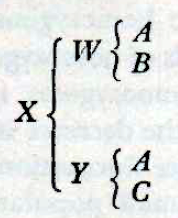
\includegraphics[width=0.3\textwidth]{Page_273.png}
    \label{fig:Lush_Figure_Page-273}
\end{figure}

\noindent
\textit{W} and \textit{Y} are related to each other 25 per cent, and
\(F_X = 12.5\) per cent or \nicefrac{1}{8}. The one line of descent connecting
\textit{W} and \textit{Y} is \(W \leftarrow A \rightarrow Y\). To
see what will probably happen to the genetic composition of \textit{X}, we will
consider a pair of genes, \textit{Rr}, for which \textit{A} is heterozygous.
What is the probability that \textit{X} is homozygous (\textit{RR} or
\textit{rr}) through having received duplicate genes in this locus from
\textit{A}? We are not interested in genes
from \textit{B} or \textit{C} since, as far as the pedigree shows, they are unrelated to
each other or to \textit{A}, and our inbreeding coefficient measures only how
many of the genes heterozygous in the foundation animals (those at the
base date to which the inbreeding was computed) have probably
become homozygous in \textit{X} because of its inbreeding. \textit{W} and \textit{Y} are each
equally likely to have received \textit{R} or \textit{r}. They each are equally likely to
transmit whichever gene (\textit{R} or \textit{r}) they did receive from \textit{A}, or the allel to
it which each received from its other parent. The probabilities with
respect to the genes of the \textit{Rr} pair in \textit{X} are as follows:
\begin{align*}
 ~&\text{4 chances in 16 that neither gene came from } A\text{.} \\
 ~&\text{4 chances in 16 that } R \text{ came from } A \text{ but the other allel came from a
grandam.} \\
 ~&\text{4 chances in 16 that } r \text{ came from } A \text{ but the other allel came from a
grandam.} \\
 ~&\text{2 chances in 16 that both genes came from } A \text{ and } X \text{ is } Rr\text{.} \\
 ~&\text{1 chance in 16 that both genes came from } A \text{ and } X \text{ is } rr\text{.} \\
 ~&\text{1 chance in 16 that both genes came from } A \text{ and } X \text{ is } RR\text{.}
\end{align*}

\noindent
If either of the last two events happened, \textit{X} is homozygous for a gene
for which \textit{A} was heterozygous. Together the last two events have a
probability of one-eighth of happening. When we say that the inbreeding
coefficient of \textit{X} is \nicefrac{1}{8}, we are saying that \textit{X} is probably homozygous
for \nicefrac{1}{8} of the genes which were heterozygous in the ancestors at the
foundation or base date to which the pedigree of \textit{X} was traced. If we
combine the probabilities of each of the above events happening, and
include also what would have happened if \textit{A} had been \textit{RR} or \textit{rr}, we
find that if many are bred like \textit{X} (i.e., with the inbreeding
that results from being double grandsons) from a population of grandparents
whose zygotic frequencies\index{Zygotic ratios} are: $q^{2}RR : 2q(1 - q)Rr : (1-q)^{2}rr$,
then the most probable zygotic ratio among those bred like \textit{X} is:
$[q^2 + Fq(1 - q)]RR : 2q(1 - q)(1 - F)Rr: [(1 - q)^{2}+Fq(1 - q)]rr$.
In other words this amount of inbreeding will probably transform \nicefrac{1}{8}
of the heterozygous gene pairs into homozygous ones, half of that \nicefrac{1}{8}
being added to each of the two kinds of homozygotes. Thus the inbreeding
is impartial between the two homozygotes, tending on the average
to add to each of them one-half of the decrease it causes in the frequency
of heterozygotes. Of course chance fluctuations concerning that fraction
are large in the necessarily small population which is any one
inbred line.
\index{Sampling nature of inheritance|)}

The measurement of inbreeding, even in the most complicated pedigrees,
is simply computing the amount of heterozygosis probably lost
because of the inbreeding. In the simpler cases, where sire and dam are
related through only one or two lines, the computations are easy. It is
only necessary to find the common ancestor, count and add the number
of segregations between sire and ancestor and between dam and ancestor
and compute \nicefrac{1}{2} to one higher power than that. If much of this is to
be done, it is convenient to memorize or have handy a table of (\nicefrac{1}{2})$^n$ for
values of \textit{n} from 1 to 7 or 9. When \textit{n} is more than 6, this fraction is less
than 1 per cent. Little is gained by investigating any one relationship
too distant to contribute even this much, although if there are very
many such lines, their total might be important.

In the more complicated cases it may be necessary and is convenient
to draw the pedigrees in the arrow style shown in the middle and bottom
of Figure~\ref{fig:Lush_Figure_35}. In this form of pedigree each ancestor is shown only
once. An arrow leads from it to each descendant. Unless it had more
than one descendant it did not provide any inbreeding itself, but merely
transmitted to its one offspring some of the genes received from its
parents. When pedigrees are drawn in arrow style it is usually easy to
see at a glance what kind of a breeding system had been used and
toward which ancestors the inbreeding had been directed. Printing
difficulties are an obstacle to using the arrow style widely, as well as the
fact that in most pedigrees in sale catalogues and advertisements there is
little or no inbreeding visible, and in many cases the owner does not
wish to call attention to that small amount. At the bottom of Figure~\ref{fig:Lush_Figure_35}
are shown the computations for the amount of inbreeding coming from
each line through which sire and dam are related.

\begin{figure}
	\centering
    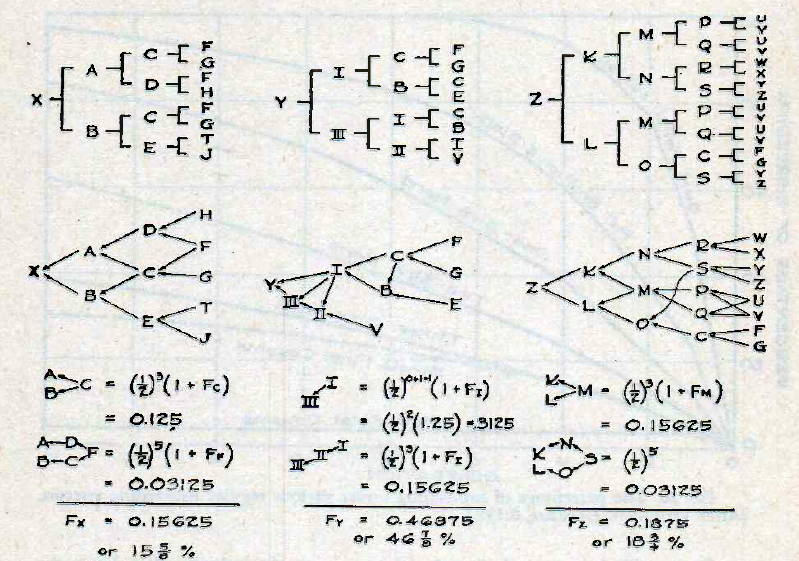
\includegraphics[width=\textwidth]{Figure_35.png}
    \caption{Three pedigrees illustrating how the coefficient of inbreeding is computed.}
    \label{fig:Lush_Figure_35}
\end{figure}

In pedigrees from experiments where inbreeding has been conducted
for many generations, the computations may become very intricate.
Occasionally that happens in purebreeding where, as in the case of
the ``straightbred'' Anxiety 4th Herefords, a family has been bred with
little or no outside blood for more than five or six generations. For
practical purposes it is usually sufficient in such cases to compute the
inbreeding for only the last four or five generations and assume that the
ancestors at that date were typical of this family, thus making the coefficient
relative to this family at that date instead of making it relative to
the whole breed.

Figure~\ref{fig:Lush_Figure_36} shows for some regular inbreeding systems the sharp differences
between the most intense systems theoretically possible and
some of the milder ones which might more readily be practiced with
farm animals. The milder inbreeding systems are much less intense at
the start but if continued long enough in an entirely closed population
can bring the population to a high degree of homozygosis. How very
long that would be in terms of one breeder's lifetime can be seen by
multiplying the number of generations in Figure~\ref{fig:Lush_Figure_36} by two and one-half
years in the case of swine, four or five years in the case of cattle and
sheep, and ten or more years in the case of horses.

\begin{figure}
	\centering
    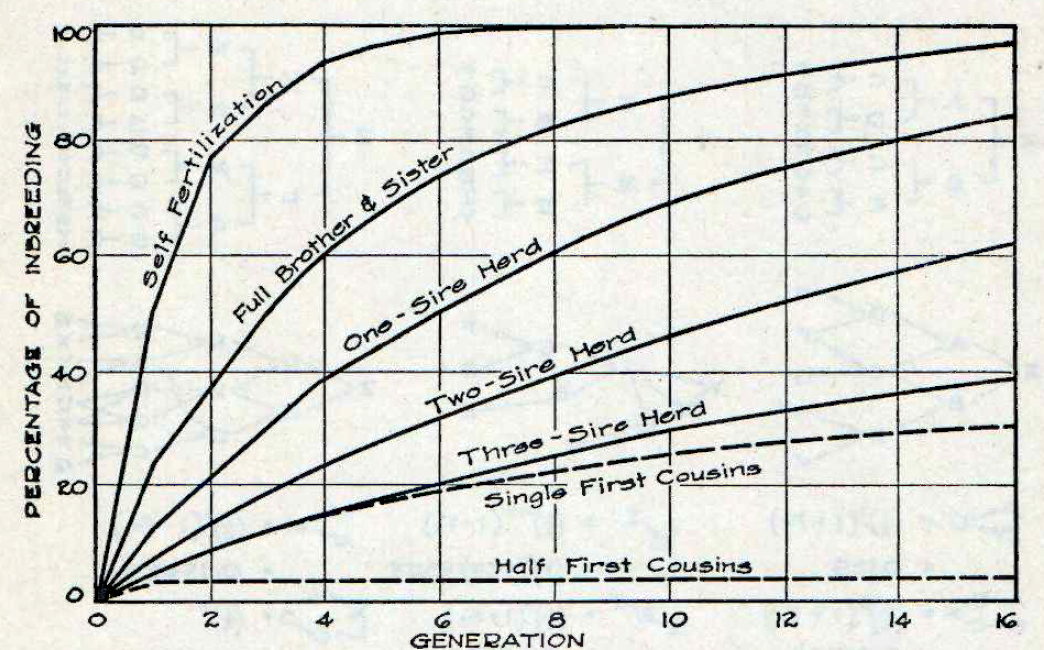
\includegraphics[width=\textwidth]{Figure_36.png}
    \caption{The percentage of inbreeding under various regular inbreeding systems.
(After Wright in Genetics, 6:172.)}
    \label{fig:Lush_Figure_36}
\end{figure}

Figure~\ref{fig:Lush_Figure_37} shows similarly what happens to the relationship between
full brothers under the same inbreeding systems. Unrelated families
are apt to drift farther apart under inbreeding than they would under
random mating, but each tends to become uniform within itself. A one-sire
herd where no females are ever purchased but each new sire is
unrelated to the herd will approach but never rise above the level of an
average relationship of 33\nicefrac{1}{3} per cent between herd mates. By contrast
a one-sire herd in which neither sires nor dams are purchased and there
is no overlapping of generations will even in the first inbred generation
reach an average relationship of 39 per cent between herd mates and in
the next generation will pass 50 per cent. The whole herd will then be
more uniform than if all members were full sibs.
\index{Inbreeding!measurement of|)}

\begin{figure}
	\centering
    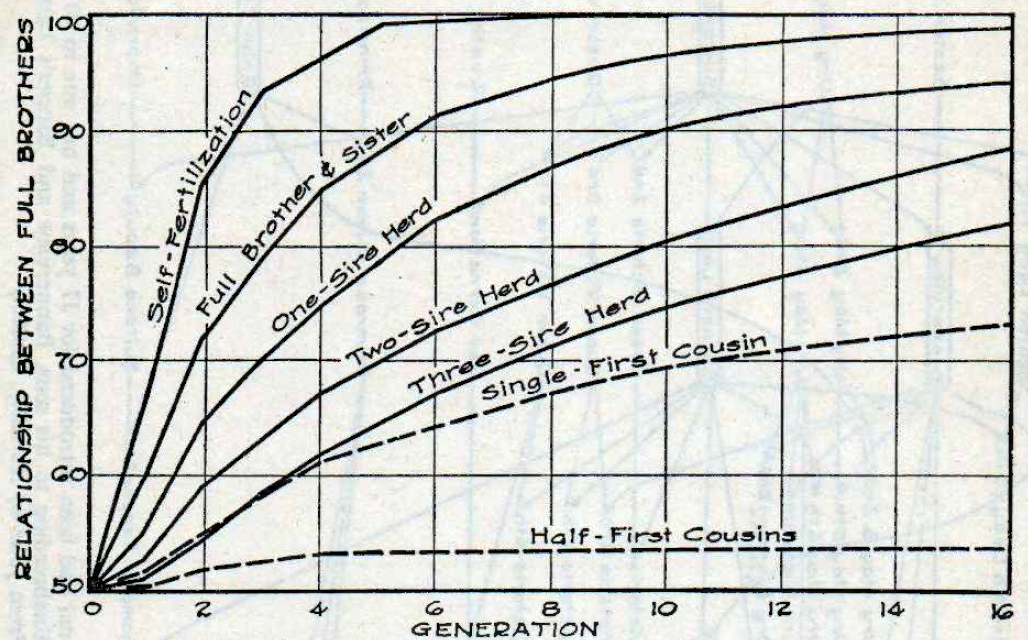
\includegraphics[width=\textwidth]{Figure_37.png}
    \caption{The relationship between full brothers under various regular inbreeding
systems. (After Wright in \textit{Genetics}, 6:170.)}
    \label{fig:Lush_Figure_37}
\end{figure}

\section*{THE RATE OF INBREEDING IN ISOLATED POPULATIONS}
\index{Inbreeding!in isolated populations|(}

The complete formula for the inbreeding coefficient is unwieldy in
estimating the consequences of any breeding plan which is to extend for
more than a few generations. For example, one might have a herd of
cattle just big enough to justify keeping two sires at a time; and he
might plan to raise his own sires without ever introducing any new
stock from other herds. Soon his sires would be related to all the females
on which they were to be used, but this relationship would vary. Many
would be half sisters, some would be cousins, some would be less closely
related older cows from the preceding generations, a few might be full
sisters, dams, three-quarter sisters, etc. Figure~\ref{fig:Lush_Figure_38}
shows an actual exam ple of this from a Shorthorn herd where only one sire
and no females 	had been bought in 20 years.\footnote{\textit{Jour. of Heredity},
25:208--16.} To compute the average inbreeding in
such an actual herd after it has been produced is a tedious job and not
very practical, since the animals are already produced whether one
likes them or not. For practical purposes one wants to estimate and
compare the consequences of various possible plans, so that the one
thought most favorable can be adopted and the less favorable ones left
untried.

If a population is kept entirely closed to outside blood, about
\(\dfrac{1}{8M} + \dfrac{1}{8L}\) of the remaining heterozygosis will
be lost per generation, where \textit{M} is the number of males and
\textit{L} is the number of females reaching breeding age in each
generation.\footnote{For the derivation of this formula see: \textit{Genetics},
16: 107--11. Strictly speaking, \textit{M}
and \textit{L} are the ``effective numbers.'' They would equal the actual census numbers in
the simple case in which all males and all females had equal chance to leave offspring.
Many conditions can cause the effective numbers to be smaller than the actual
numbers. At least a few of these will occur in practice. Hence the formula will
underestimate the amount of inbreeding in closed populations. See \textit{Amer. Nat.}, 74:241--47. 1940.} In a herd where there are 2 sires
and 40 females in active use, this would be \nicefrac{1}{16} + \nicefrac{1}{320}, or about 6.6
per cent of the remaining heterozygosis. In animal breeding, \textit{L} will
usually be so much larger than \textit{M} that the term $\dfrac{1}{8L}$ can be neglected
without much error. Then the formula becomes simply $\dfrac{1}{8M}$ giving
inbreeding rates of 12 per cent, 6 per cent, 4 per cent, and 3 per cent per
generation, respectively, for one-sire herds, two-sire herds, three-sire
herds, and four-sire herds, closed to all outside blood. These rates can
be reduced somewhat by avoiding inbreeding as far as possible under
those conditions. No reduction at all could be produced in a one-sire
herd, only a small reduction in a two-sire herd, more in a three-sire
herd, etc. The maximum effect of avoiding all inbreeding as far as possible
within a closed population tends toward halving the rate given by
the formula.

\begin{figure}
	\centering
    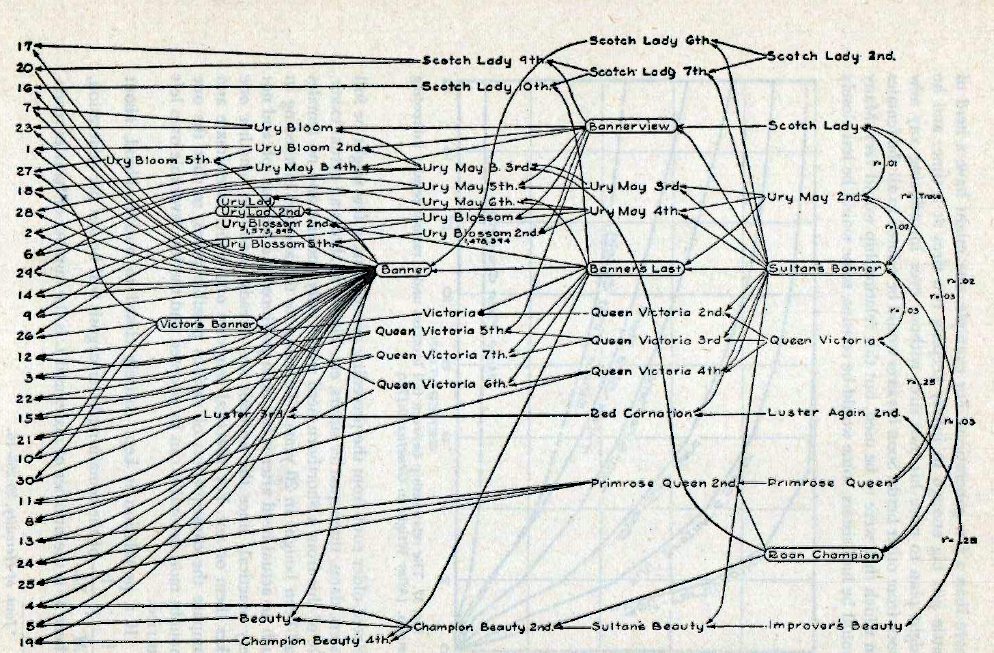
\includegraphics[width=\textwidth]{Figure_38.png}
    \caption{Pedigree of a Shorthorn herd in which no animal had been introduced for 17 years and but 
    		 one in 20 years. The herd was built largely around Sultan's Banner with some secondary 
    		 linebreeding to his sons, Bannerview and Banner's Last and quite a bit of
			 secondary linebreeding to his double grandson, Banner. (From \textit{Jour. of Heredity}, 
			 25:208.)}
    \label{fig:Lush_Figure_38}
\end{figure}

By this formula we can calculate where purebred systems with rigidly
closed herdbooks are drifting, so far as concerns any inbreeding
which is inevitable because the members of a pure breed are becoming
more closely related to each other. Even in a small breed with 200 sires
and 2,000 dams used per generation, the formula shows only .069 per
cent of the heterozygosis lost per animal generation. In other words it
would take about 15 animal generations to lose 1 per cent of the remaining
heterozygosis in such a small breed. There need be no fear that a
closed herdbook will automatically lead to dangerously high inbreeding,
even though the herdbook remains closed and the breed remains
moderately small for centuries. However, show rings, advertising, and
other sales efforts make some males more popular than others. These
males have many sons and grandsons which go to head other registered
herds. Less popular sires have no sons which see service in purebred
herds and perhaps few daughters and no grandsons. This has the effect
of making \textit{M }in the formula much smaller than the actual number of
males which have registered daughters in each generation. In several
pure breeds so far studied, the decrease in heterozygosis per generation
on account of the inbreeding practiced is not very far from 0.4 to 0.6 per
cent. Even so, only about 10 to 12 per cent of the present amount of
heterozygosis would disappear in another century of pure breeding like
that of the last 30 years. An occasional undetected fraudulent registration
of a grade would further reduce this rate.
\index{Heterozygosis|)}
\index{Inbreeding!in isolated populations|)}

\section*{COMPLETE FORMULA FOR THE MEASUREMENT OF RELATIONSHIP}
\index{Relationship!measurement of|(}

The measures of relationship can now be corrected for the effects of
inbreeding. The complete formula for the coefficient of relationship
between animals \textit{X} and \textit{Y} is:

\[R_{XY} = \frac{\Sigma[{1/2}^n(1 + F_A)]}{\sqrt{1 + F_X}\sqrt{1 + F_Y}} \]

\noindent
where \textit{n} is the total number of Mendelian segregations in the path of
descent through which \textit{X} and \textit{Y} are related. This differs from the
approximate formula used in the last chapter only by having terms for
the inbreeding of \textit{X} and \textit{Y} and of their common ancestor. The $(1 + F_A)$
in the numerator allows for the fact that an inbred ancestor (\textit{A}) is
homozygous for more pairs of genes than a non-inbred one. Its use is
illustrated in Figure~\ref{fig:Lush_Figure_35} where the inbreeding of I adds to the relationship
betwen itself and III, or the inbreeding of \textit{M} increases the relationship
between \textit{K} and \textit{L}. The terms in the denominator are to correct for
the fact that inbreeding makes the population more variable, the inbred
lines tending to drift apart from each other. Relationship is a fraction
which has for its numerator the number of genes in which the two
related animals are probably alike but which would be unlike in two
random animals from the base population, and for its denominator the
average number of genes in which two animals probably would be
unlike if they were unrelated but descended from the base population
by the same kind of breeding system as the two actually are. The
denominator grows larger with their inbreeding because the inbreeding
tends to decrease the proportion of heterozygosis and to throw the
population toward the two homozygous extremes in each pair. In a
highly inbred population two unrelated individuals (necessarily from
different inbred lines if they are unrelated) have a considerably larger
chance of being \textit{AA} and \textit{aa} than if they were from a non-inbred population,
because in the inbred population there are more \textit{AA} and \textit{aa} and
fewer \textit{Aa} individuals present. This increase in the denominator naturally
lowers the relationship unless there is a corresponding or greater
increase in the numerator. Such an increase in the numerator can and
usually does occur if the two animals are members of the same inbred
line but not if they belong to lines which have separated and no longer
interbreed with each other.

The complete formula for relationship between an animal and its
ancestor where there is no collateral relationship may be written

\[ R_{XA} = \Sigma[{1/2}^n]\sqrt{\frac{1 + F_A}{1 + F_X}} = \text{``Percentage of blood'' times }\sqrt{\frac{1 + F_A}{1 + F_X}} \]

\noindent
If \textit{A} and \textit{X} are equally inbred, the term under the square root sign
equals 1.0 and the percentage of blood is exactly equal to the coefficient
of relationship. If the ancestor is more highly inbred, the figure for percentage
of blood is not quite large enough. This is because there will be
more than the average number of cases in which the ancestor is homozygous
and therefore both its genes in that pair will be like the one its
descendant receives from it. If the descendant is more highly inbred, the
figure for percentage of blood is a little too large. This is because there
will be cases in which the descendant is homozygous for a gene heterozygous
in the ancestor. In such gene pairs the descendant gets 100 per
cent of its genes from that ancestor and yet is not 100 per cent like the
ancestor. For an example we may return to the pedigree of \textit{X}
(page \pageref{fig:Lush_Figure_Page-273})
which was a double grandson of \textit{A}. In one-fourth of the cases for any
one pair of genes, \textit{X} gets both its genes from the grandams and none
from \textit{A}; in one-half the cases, \textit{X} gets one gene of the pair from \textit{A} and
the other from a grandam; in the remaining one-fourth of the cases, \textit{X}
gets both genes from \textit{A}. On the average, therefore, \textit{X} gets 50 per cent of
its inheritance from \textit{A}, just as the percentage of blood figure shows.
However, in the one-eighth of the cases when \textit{X} is \textit{rr} or \textit{RR}, it will get
both genes from \textit{A} but yet will not be exactly like him, because he was
\textit{Rr}. The corrections in the denominator thus keep the relationship
coefficient a measure of probable genetic likeness and not merely a
measure of source of the genes, as is percentage of blood. Not often is
the difference in the inbreeding of \textit{A} and \textit{X} large enough to be important.
A much more serious general defect of percentage of blood as a
measure of relationship is that it does not include collateral relation ship
and that collateral relationship cannot readily be measured by any
way of manipulating percentage of common blood.

In the pedigrees ordinarily encountered in actual animal breeding,
the denominator of the relationship coefficient does not get very much
larger than 1.0. Neglecting it altogether is not apt to lead to a serious
mistake. However, it must be included if the formula is to be entirely
correct. It is not often worthwhile to carry the computation of either
\textit{R} or \textit{F} for individual animals farther than to the nearest 1 per cent.
Often the nearest 5 per cent is close enough. The sampling variations
inherent in Mendelism prevent one from being sure that the computed
coefficient describes with extreme accuracy the actual situation in individual
cases, even if one could make practical use of small differences
in these coefficients.

The similarity between the formula for inbreeding and the complete
formula for relationship shows how it is that an individual's
inbreeding depends upon the relationship between its sire and its dam.
The equations connecting the two, where \textit{S} represents the sire, \textit{D} the
dam, and \textit{O} the offspring, are:

\[ F_O = \frac{R_{SD}}{2} \times \sqrt{(1 + F_S)(1 + F_D)}, \text{and} \frac{R_{SD}}{2} = \frac{2F_O}{\sqrt{(1 + F_S)(1 + F_D)}} \]

\noindent
Unless the sire and dam are highly inbred, the term under the square
root sign will not differ much from 1.0; and it will be approximately
correct to say that the inbreeding of the offspring is one-half of the relationship
between its parents. This rule is useful when estimating the
amount of inbreeding danger in a mating before that mating is made.
\index{Relationship!measurement of|)}

\section*{OTHER PROCESSES WHICH CAN AFFECT HOMOZYGOSIS}

The inbreeding coefficient expresses probable changes in homozygosis
based on no other assumptions than that inheritance is Mendelian
and is equal from the two parents. It neglects sex-linkage\index{Sex linkage} and the small
changes in homozygosis which may be made by mutation and selection
and by assortive mating which is not inbreeding.

So far as concerns sex-linked genes, the inbreeding coefficient for the
pedigree of a heterogametic animal has no meaning. The heterogametic
parent behaves as if it were entirely homozygous for sex-linked
genes in transmitting to its homogametic offspring, and transmits no
sex-linked genes at all to its heterogametic offspring. Referring for convenience
to the female as the homogametic sex (as is correct for the
mammals but not for the birds and a few other animals), the inbreeding
computed for a female's pedigree is not true for her sex-linked genes
wherever the line of descent is from sire to son. On the other hand,
wherever the line of descent is from sire to daughter, the homozygosity
of females for sex-linked genes will be higher than the coefficient indicates.
These two effects tend partly to cancel each other so that the
inbreeding coefficient will generally measure the extra homozygosity of
females, even for sex-linked genes. There will be cases where the coefficient
will be systematically in error for the sex-linked genes; e.g., a
double granddaughter of a male would not tend to have her sex-linked
genes any more homozygous than if her parents had been unrelated,
while a double granddaughter of a female would have her sex-linked
genes 25 per cent less heterozygous instead of the expected 12½ per
cent.\footnote{A more detailed explanation of the consequences of inbreeding on
the distribution of sex-linked genes was presented by Wright in 1955.
\textit{Proc. Nat. Acad. Sci.}, 19:411--20.}

Mutation\index{Mutations} is so rare an event that its neglect in the formula introduces
no error of importance in practical breeding, although mutation
needs to be included in evolutionary considerations where the time
involved extends over an enormous number of generations. The formulas
for including it are rather intricate.\footnote{\textit{Genetics}, 16:116--37.}

\index{Selection!and homozygosis}
Selection affects homozygosis only incidentally through changing \textit{q}
and thereby the value of $2q (1 - q)$. Selection will usually require many
generations to make large changes in \textit{q}, except in those cases where
intense selection is directed at a characteristic the main variations of
which are highly hereditary and are determined by a very few genes.
The effects of :;election on homozygosis certainly need to be considered
in connection with problems of evolution, but in general they are
probably too small to make inbreeding coefficients much in error as
measures of the change in homozygosis which has occurred within the
last four to six generations. Assortive mating (as will be explained in
chapters 27 and 28) has almost no effect on homozygosis except when
(l) the assortive mating is almost perfect, (2) the characteristics concerned
are highly hereditary, and (3) the number of genes producing the
observed variation is small. Very rarely would all these conditions be
met in actual practice.

\section*{PRACTICAL USES OF INBREEDING}
\index{Inbreeding!practical uses of|(}

Most breeders inbreed only when they must to attain some other
object, such as linebreeding or forming and preserving family distinctness.
The commonest reason for inbreeding is that a breeder must do
some of it if he is to keep his animals closely related to individual animals
he admires. Relationship between two animals cannot go higher
than 50 per cent unless there has been some inbreeding. If a breeder
continually uses unrelated sires, the relationship of each succeeding
generation to the animals he has had in his herd will be halved. In a
short time his animals will be very little related to the best ones of two
or more generations ago. If he still has a good herd, that will be because
he has been successful in selecting his subsequent sires. If, instead of
using unrelated sires each generation, he uses sires closely related to the
best animals he has had, then he may keep the future generations as
closely related to those good ancestors as his present animals are. But,
since both sires and dams of his stock are related to these good animals,
he will be practicing some inbreeding. This is the essence of ``linebreeding,''
which is the subject of Chapter 23. In this practice most breeders
regard inbreeding as a necessary evil which must be endured if they are
to keep their herd closely related to some noted animal, but which
should be kept as low as can be done and still accomplish the linebreeding
program.

If the homozygous recessives can all be discarded, inbreeding can be
a powerful help to selection against rare recessives. There may be so
many recessives in the stock that the inbreeding will bring them to light
in more animals than the breeder can afford to discard, or he may not
recognize some of those with the less conspicuous effects in time to discard
them before they become fixed on his whole herd. This is what
breeders have in mind if they say that their breed is not yet perfect
enough to make even linebreeding wise as a general policy. The price
which must be paid for using inbreeding thus to improve the breed is
the occurrence at first of a larger proportion of undesirable individuals.
That price may be so high that the individual breeder will not find it
economically possible for him to practice extremely close inbreeding as
a steady policy.

Inbreeding may be used to test whether animals are good enough to
justify deliberate and long-continued attempts to keep the herd closely
related to them. Inbreeding is the severest test of the hereditary worth
of an individual that can be made. Wriedt goes so far as to recommend
that every dairy bull thought worth using in the first place should be
bred as soon as possible to enough of his daughters to insure that there
will be at least 15 or 20 of his daughters out of his own daughters to
prove his breeding value. For several reasons this proposal seems too
extreme for general adoption. However, it does rest on the truth that
inbreeding is the severest and quickest test to find whether an animal
has any undesired genes.

Inbreeding can be used to promote homozygosity. Homozygosity has
little commercial value in the sale ring as yet. Hence it seems unlikely
that many breeders could afford to inbreed intensely just for this object.
Nevertheless, homozygosity is the most important element in prepotency,
and the building of this into his herd is worth some effort by the
breeder, provided he can maintain or improve the average phenotypic
merit at the same time.
\index{Homozygosis|)}

A breeder often practices inbreeding merely for economy. This is
an unwise policy whenever the animals are of only average merit. He
could then expect only offspring of average merit, even if there were no
inbreeding. With the added probability of some phenotypic degeneration
from inbreeding, he can expect the offspring to be below the average
merit of their breed as individuals, although not necessarily below
the breed average in their merit as breeding animals. When the animal
to which the inbreeding is being directed is of superior merit, this reason
of economy lends additional weight to the argument for inbreeding.

One of the important general reasons for practicing inbreeding is
that it tends to form distinct families within the breed and thus permits
more selection between families than would be possible under random
breeding. (This will be discussed in more detail in Chapter 24). Selection
between families can be much more accurate than selection
between individuals, especially for characteristics which are only slightly
hereditary; but the families must be rather distinct from each other if
that is to be the case. The family averages of non-inbred families do not
deviate from each other as much as individual genotypes do.

The producer of market animals has little reason to practice
inbreeding. His market will not pay him any extra for prepotency.
Improvements he may make in the average merit of his own herd by
using inbreeding along with selection will be about halved next time he
buys an unrelated sire from some other source, as most commercial producers
do. Economy can be a valid reason with him, especially when he
thinks the sire he has is better than the next one is likely to be. Partly
offsetting this superiority of his present sire is the probability that
some harmful results of inbreeding will occur in his herd.)
\noclub
\index{Inbreeding!practical uses of|)}

\section*{THE DANGERS OF INBREEDING}
\index{Inbreeding!dangers of|(}

Inbreeding makes desirable and undesirable genes homozygous
impartially. If the rate of this is too rapid, every individual produced
will be homozygous for some undesired genes as well as for some desired
ones\index{Variation!increased by inbreeding}. If the inbreeding is too mild, many generations will be needed to
accomplish much with it. The problem of the best rate at which to
inbreed is one of keeping the inbreeding mild enough that the man in
charge can avoid fixing the genes with undesirable effects and can fix as
many as possible of the genes which have desirable effects. How mild or
how intense such inbreeding can be depends upon several things, the
most important of which are the skill of the man doing the selecting,
the abundance of undesired genes in the stock with which he begins, the
amount of linkage between desired and undesired genes in the initial
stock, the amount of epistasis, dominance, or environmental effects
which may deceive the breeder when he makes his selections, and
whether he is breeding a group all by himself. If other men are breeding
closely related lines, he can correct his mistakes by mild outcrosses
to some of their herds without having to use totally unrelated animals.

Fragmentary evidence of various kinds indicates that inbreeding
rates as high as 6 per cent per generation\footnote{As, for example,
in a two-sire herd where no outside blood is introduced.} under favorable
circumstances may be pursued for many generations without noticeably
harmful consequences. It is unlikely that inbreeding rates as high as 3 or 4
per cent can go on forever without harm, but certainly they can be continued
for many generations. Many breeders when in possession of
unusually good animals have had favorable results from mating half
brother to sister or grandsire to granddaughters, but not many have
continued to do that for more than two or three successive generations.
Occasional matings of parent and offspring or, more rarely, full brother
and sister have turned out well; but general experience is that those
should be risked only when the stock is unusually good.

Among human beings inbreeding as intense as the marriage of first
cousins has enough probability of undesired consequences that in some
places it is forbidden by law or religious rule.\footnote{See page 52
of \textit{Time} for August 19, 1940, for a list of marriages forbidden by the
Church of England in 1560. In 1945 prohibitions against ten of these categories of
in-law marriages were removed. This was the first change in those rules in nearly
four hundred years.} Inbreeding more intense
than that is regarded as ``incest'' in nearly all human societies although
there have been some exceptions, as among the Pharaohs in ancient
Egypt. No doubt the biological principles are the same in man as in
other organisms, although the abundance of undesired recessives may
be higher or lower. An extremely important practical difference is that
in farm animals, if inbreeding brings to light a few more defectives
than would occur without it, they may be culled with only the small
economic loss that their defectiveness entails; whereas in most civilized
communities of man the codes of ethics and morals do not permit such
drastic action with defective human beings. The care and support of
each one too defective to take care of itself is a serious burden, whether
it is kept in a private home or in a special institution. Rigid prohibitions
of marriages of a certain degree, such as between first cousins, do
not allow for the fact that such marriages may be desirable when the
common ancestry is of unusual merit. Prohibiting the marriage of relatives
does not improve the average heredity of a population. Neither
inbreeding nor outbreeding makes the undesired genes systematically
either rarer or more abundant, but inbreeding does bring them together
so that more of them can show their effects and be culled-if selection
is being practiced. Perhaps the general experience of man over centuries
may be considered as indicating that around 6 per cent is in general
the ``stop, look, and listen'' level of danger from inbreeding? If the
common ancestry is of sound stock, the children of such marriages may
be above average in merit. If the common ancestry has any serious
defect, even a rare one, the probability of that defect reappearing in the
children who have a chance to inherit it from both sides is much higher
than if their parents were unrelated. The rarer the defect in the general
population, the more extreme is this difference.

The inbreeding coefficient may be used to estimate the danger
involved in any particular mating, if one considers also the merit of the
ancestors from which the inbreeding comes. Inbreeding of 25 per cent
coming from an outstanding ancestor might be safer than inbreeding of
10 per cent coming from a mediocre ancestor. Setting a definite percentage
of inbreeding as the point where danger begins is much like
setting a certain speed in automobile driving as the speed beyond which
danger begins. In the case of the automobile much depends upon the
condition of the highway, the field of vision, the mechanical condition
of the car and the skill of the driver. Similarly with inbreeding, much
depends upon the clearness of the goal, the accuracy of the tests and
measures of merit, the initial scarcity of undesirable genes in the stock,
the amount of culling which the reproductive rates permit, and the
breeder's ability to recognize and discard genes which are on the verge
of becoming fixed in his stock.
\index{Inbreeding!dangers of|)}

\section*{POSSIBILITIES OF PRODUCING INBRED LINES FOR COMMERCIAL CROSSING}

Corn breeders have made a distinct success of producing inbred
lines by self-fertilization and then crossing those lines which produce
the most desirable crosses. The crossbred seed is sold for the production
of commercial corn. Although the fundamental principles are the
same, there are several differences in their application which make the
success of such a breeding system appear less likely for animals than for
plants, although modified systems based on the same principles may
perhaps prove successful. In the first place, the closest possible inbreeding
in animals is less than half as intense as self-fertilization. It would
take many more generations with animals to reach the same degree of
homozygosity. In the second place, the fertility of animals is lower than
that of plants, so that not nearly as large a percentage of the individuals
produced in each generation could be discarded. In the third place,
the interval between generations in farm animals is longer than with
annual plants; and the amount of time required to reach an equal
degree of inbreeding would be longer for that reason also. In the fourth
place, the individual animal is worth more money than the individual
plant. Culling the undesired individuals which appear during the
inbreeding will be more expensive than the same process applied to
plants. In the fifth place, and partially offsetting these others, is the fact
that the merits and faults of individual animals are usually better
known than is the case with individual plants. Therefore, the individual
selection which accompanies the inbreeding would be more
accurate in animals. In the sixth place, the lower fertility of animals
would make it economically difficult to sell the commercial producer as
many as he would need of the crossbred stock from two successfully
inbred lines, if such should ever be produced, or to sell him inbred
females of one line and inbred males of another line so that he could
make his own crosses. Poultry and swine seem more nearly suited to the
economics of that than the other farm animals.

For those reasons commercial animal breeding will never practice
such intense inbreeding alternating with such extreme outbreeding as
is already practiced in corn breeding. On the other hand, a mild form
of this is already happening in the crossbreeding which is practiced for
producing commercial meat animals and in the practice, among breeders
of purebred stock, of making outcrosses between distinctly unrelated
lines within a breed, hoping thereby to produce excellent individuals.
Perhaps it may be commercially possible to produce highly inbred sires
to be used on practically random-bred high grade or purebred females.
At present stockmen set so much store by individuality in their sires
that few of them would use inbred sires unless these were also good
individuals, but that would change quickly if it were demonstrated
clearly that such use would be profitable.

\section*{EXPERIMENTS ON INBREEDING}

Thorough and extensive experiments on inbreeding have been
more numerous with plants than with animals. Many of the facts
about inbreeding were discovered in experiments with corn. More come
from the contrasting behavior of naturally self-fertilized and naturally
cross-fertilized plants when those are experimentally inbred or are used
in various crosses. Conspicuous examples of plants which in nature
have a high percentage of self-fertilization include wheat, cotton, sorghum
and oats. Corn and beets are examples of naturally cross-fertilized
species on which extensive experiments with inbreeding have led to the
production of inbred lines and the sale of crossbred seed on a commercially
important scale. Strawberries and raspberries show much the
same results as corn and beets, but the application is different because
vegetative multiplication of the former is practical.

Among animals, laboratory experiments have been extensive on the
inbreeding of rats, mice, and guinea pigs. Dr. King inbred white rats
full brother and sister for more than 70 generations without finding
degeneration. Mice have been inbred full brother and sister in many
experiments. In at least one case this has been carried further than the
55th generation.\footnote{\textit{Jour. of Heredity}, 27:21--24, 1936.}
In the United States Department of Agriculture
experiments on inbreeding guinea pigs, some lines have been inbred
brother by sister for more than 30 generations. There have been several
short experiments on inbreeding chickens and swine at a number of
experiment stations. In 1945 the 38 lines being studied in the Regional
Swine Breeding Laboratory ranged from about 10 to 70 per cent in
inbreeding. Twelve of them were already inbred more intensely than
three generations of full brother by sister and ten more were nearly that
far along. Inbreeding experiments with poultry at the Iowa Station
have reached a more intense stage than that of nine generations of full
brother by sister mating, although the breeding system actually used
was not that regular.

In farm animals other than chickens and swine, the small number of
full sibs and the variations in the sex ratio prevent the long-continued
use of such regular inbreeding systems as full brother by sister. Even in
chickens and swine these are serious difficulties and reduce tremendously
the amount of selection which can be practiced while the inbreeding
is being done. For the other farm animals the most intense inbreeding
plan which can be followed long is the use of a sire on his daughters as
long as he lives, he to be followed by one of his inbred sons, which in
turn would be followed by one of his inbred sons, and so on. There
would be a few full brother by sister matings and some of the females
would live longer than others, some, perhaps, even outliving two generations
of sires. Hence such a system of inbreeding would be far from
regular, and there would be comparatively few pedigrees which were
exactly alike in the kinds of inbreeding they showed over a period of
three or four generations. Before an inbreeding coefficient was devised
for measuring the intensity of the irregular inbreeding shown in these
many kinds of pedigrees, it was natural that experimenters should think
that inbreeding experiments of that kind could not be interpreted in
any unmistakable way and therefore would not return scientific information
worth the money and effort they would cost. Now that Wright's
coefficient of inbreeding, which was first proposed in 1922, largely
removes this objection, it is probable that more experimental study will
be made of irregular systems of inbreeding.

Some of what we know about the results of inbreeding in animals
comes from the scattered and irregularly reported experience of breed ers.
It is difficult to be at all sure that such evidence is a typical sample
of the results of inbreeding. There is the question of whether the animals
inbred were typical of purebred animals in general. There is also
the question of whether one hears of the typical results of such cases or
only of the exceptional results. Any bad result which does appear is apt
to be blamed on the inbreeding in spite of the fact that equally bad
results sometimes occur when no inbreeding is practiced. There is
usually an absence of adequate control; that is, of non-inbred animals
kept under the same conditions. However, the results agree in general
with those expected on theoretical grounds and with those actually
obtained in laboratory experiments. The usual consequences of
inbreeding in breeders' experiences is a degeneration which, however,
is slight and irregular, affecting some characteristics in one animal and
other characteristics in another and not affecting some individual animals
at all. Even in Bakewell's time it was known and stressed that
inbred animals are more apt to be prepotent and effective when used in
outcrosses than are animals of equal individuality but not inbred.

The breeders who have practiced intense inbreeding for a long time
have nearly always encountered enough degeneration that a cross with
unrelated animals produced beneficial results. So universal has this
experience been that breeders are rather generally convinced of the
necessity of introducing ``fresh blood'' from time to time to ``rejuvenate''
a strain or herd. It is not always understood that this rejuvenating
effect rarely occurs unless there has been some prior inbreeding. The
explanation of these cases is that the herd becomes homozygous for
undesirable genes which produce such small effects that the breeder
scarcely notices them as they become fixed a few at a time, but instead
just sees a gradual decline in vigor, fertility, size, etc. Since undesirable
genes tend to be recessive, a cross with an animal from an unrelated
herd often appears to remedy these defects at once.

\section*{SUMMARY}

Inbreeding is the mating of animals which have a closer relationship
to each other than the average relationship within the population
concerned. Its measure is relative to some population, just as the measure
of relationship is. Pure breeding is inbreeding relative to the whole
species, but not many purebred animals are closely inbred relative to
their breed.

The primary effect of inbreeding is to make more pairs of genes
hortiozygous and to lower the percentage of heterozygosis correspondingly.
Because this uncovers many recessive genes which would otherwise
remain concealed by their dominant alleles, and because recessives
generally have less desirable effects than dominants do, there is usually
some degeneration in average individual merit when inbreeding is
practiced.

Inbreeding does not of itself change gene frequency but does permit
it to drift rapidly at random in each subgroup of the population.
Inbreeding is the most powerful tool the breeder has for establishing
uniform families or strains which are distinct from each other. This
it does by permitting gene frequencies to drift in different ways in different
subgroups, by making the parents more homozygous, and by
providing more and more ways in which members of the same family
are likely to inherit the same genes because their parents are related to
each other.

Some inbreeding is almost essential if selection is to have much success
in those cases where a highly desirable effect is produced by a combination
of genes which individually have undesirable effects; that is,
for getting a population out of some of the lower ``peaks of desirability''
shown in Figures~\ref{fig:Lush_Figure_20} and \ref{fig:Lush_Figure_21} and
into higher nearby peaks.

The coefficient of inbreeding measures the percentage of genes
which were heterozygous in the basic population but have probably
become homozygous because of the inbreeding. It is subject to the sampling
errors of Mendelian inheritance and hence means almost nothing
for one pair of genes in one individual, but its sampling error may be
small when it is applied to the average percentage of heterozygosis of
one pair of genes in a whole population or to the average heterozygosis
of the entire group of genes in one individual.

Among the more important reasons for practicing inbreeding are:
(1) It is necessary if relationship to a desirable ancestor is to be kept
high; (2) it helps uncover rare recessives so that they may be culled from
the breed; (3) it forms uniform and distinct families so that interfamily
selection may be possible in a more effective way than if inbreeding
were not practiced; (4) it increases prepotency; and (5) it is sometimes
economical, especially if the present sire is of such high merit that it
will be difficult to find as good a one for a successor.

The danger of intense inbreeding is that it will make undesired
genes homozygous at so rapid a rate that it will be impossible to discard
all individuals homozygous for them. Some of the undesired genes will
therefore become ``fixed'' in the whole herd. The lowered sale value of
the defectives uncovered by the inbreeding will cause some loss. From
the standpoint of breed improvement, that loss is balanced by the
increased prepotency of those which are not defective; but the man who
is breeding animals for the commercial market will not receive that
compensation.

It seems reasonably certain that more opportunities for breed progress
are lost by not inbreeding when inbreeding would be advisable
than are lost by too much inbreeding. When inbreeding is too intense,
the individual breeder may lose by that; but the progress of the breed
is not apt to suffer. The best of the inbred animals are likely to give
good results in outcrosses.

\section*{REFERENCES}

The general subject of inbreeding was treated comprehensively in
the following book, which, even a quarter of a century later, is obsolete
in little except its treatment of the measurement of inbreeding
intensity:

\begin{hangparas}{0.5in}{1}%
East, E. M., and Jones, D. F. 1919. Inbreeding and outbreeding. Philadelphia The
J. B. Lippincott Co. 285 pp.
\end{hangparas}

For explanation of the Mendelian basis of inbreeding and of what
happens when various rates of inbreeding, mutation, and selection are
balanced against each other, see:

\begin{hangparas}{0.5in}{1}%
Wright, Sewall. 1921. Systems of mating. Genetics, 6:111--78.

---. 1922. Coefficients of inbreeding and relationship. Amer. Nat., 56:330--38.

---. 1923. Mendelian analysis of the pure breeds o livestock. I. The measurement
of inbreeding and relationship. Jour. of Heredity, 14:339--48.

---. 1923. Mendelian analysis of pure breeds of livestock. II. The Duchess
family of Shorthorns as bred by Thomas Bates. Jour. of Heredity, 14:405--22.

---. 1931. Evolution in Mendelian populations. Genetics, 16:97--159.

---. 1940. Breeding structure of populations in relation to speciation. Amer.
Nat., 74:232--48.
\end{hangparas}

For reports of actual experiments on inbreeding animals, see:

\begin{hangparas}{0.5in}{1}%
Castle, W. E. 1930. Genetics and Eugenics, pp. 286--304. Cambridge: Harvard University
Press.

Hodgson, R. E. 1935. An eight-generation experiment in inbreeding swine. Jour.
Heredity, 26:209--17.

Hughes, E. H. 1933. Inbreeding Berkshire swine. Jour. Heredity, 24:199--203.

King, Helen Dean. 1918 and 1919. Studies of inbreeding. Jour. of Exp. Zoology,
26:1--54, 26:335--78, 27:1--36, and 29:71--112.

Strong, Leonell C. 1936. The establishment of the ``A'' strain of inbred mice. Jour.
Heredity, 27:21--24.

USDA Yearbook for 1936.

Waters, N. F., and Lambert, W. V. 1936. Inbreeding in the White Leghorn fowl.
Iowa Agr. Exp. Sta., Res. Bul. 202.

Willham, 0. S., and Craft, W. A. 1939. An experimental study of inbreeding and
outbreeding in swine. Okla. Agr. Exp. Sta., Tech. Bul. 7.

Woodward, T. E., and Graves, R. R. 1933. Some results of inbreeding grade Guernsey
and grade Holstein-Friesian cattle. USDA, Tech. Bul. 339.

Wright, Sewall. 1922. The effects of inbreeding and crossbreeding on guinea pigs.
I. Decline in vigor. II. Differentiation among inbred families. USDA,
Department Bul. 1090. III. Crosses between highly inbred families, USDA,
Department Bul. 1121.

---, and Lewis, Paul A. 1921. Factors in the resistance of guinea pigs to tuberculosis,
with special regard to inbreeding and heredity. Amer. Nat., 55:20--50.
\end{hangparas}

For brief statements of breeders' experience with regard to inbreeding,
see:

\begin{hangparas}{0.5in}{1}%
Mumford, F. B. 1921. Breeding farm animals. pp. 217--42.

Wriedt , Christian. 1930. Heredity in livestock. pp. 68--115.
\end{hangparas}

For studies of the amount and kind of inbreeding which has
occurred in various breeds of livestock, see:

\begin{hangparas}{0.5in}{1}%
Berge, S. 1930. Inbreeding in Telemark cattle. (Translated title). Nordisk Jordbrugsforskning
204--16.

Brockelbank, E. E., and Winters, L. M. 1931. A study of the methods of breeding the
best Shorthorns. Jour. Heredity, 22:245--49.

Calder, A. 1927. The role of inbreeding in the development of the Clydesdale breed
of horses. Proc. Royal Soc. of Edinburgh, 47, Part 2, No. 8, pp. 118--40.

Carter, Robert C. 1940. A genetic history of Hampshire sheep. Jour. Heredity,
31:89--93.

Dickson, W. F., and Lush, Jay L. 1933. Inbreeding and the genetic history of the
Rambouillet sheep in America. Jour. Heredity, 24:19--33.

Fletcher, J. Lane. 1945. A genetic analysis of the American Quarter Horse. Jour.
Heredity, 36:316--352.

---. 1946. A study of the first fifty years of Tennessee Walking Horse breeding.
Jour. Heredity, 37:369--373.

Fowler, A. B. 1932. The Ayrshire breed: A genetic study. Jour. of Dy. Res., 4:11--27.

L\"ortscher, H. 1945. Inbreeding and relationship among the Jura horses today.
(translated title). Landw. Jahrb. d. Schweiz, pp. 1--16.

Lush, Jay L. 1946. Chance as a cause of changes in gene frequency within pure
breeds of livestock. Amer. Nat. 80:318-342.

---, and Anderson, A. L. 1939. A genetic history of Poland-China swine.
Jour. Heredity, 30:149--56 and 219--24.

---; Holbert, J. C.; and Willham, 0. S. 1936. Genetic history of the Holstein-
Friesian cattle in the United States. Jour. Heredity, 27:61--71.

McPhee, Hugh C., and Wright, Sewall. 1925. Mendelian analysis of the pure breeds
of livestock. III. The Shorthorns. Jour. Heredity, 16:205--15.

---. 1926. Mendelian analysis of the pure breeds of livestock. IV. The British
Dairy Shorthorns. Jour. Heredity, 17:397--401.

Rottensten, Knud. 1937. Inbreeding in Danish Landrace swine. (Translated title).
Nordisk Jordbrugsforsknmg, Hefte 3--4A, pp. 94--114.

Sciuchetti, A. 1935. Ein Beitrag zur genetischen Analyse der schweizerischen Braunviehrasse.
Julius Klaus-Stiftung f. Vererb. Sozialanthr. u. Rassenh., 10:85--99.

Smith, A. D. B. 1926. Inbreeding in cattle and horses. Eugenics Review, 18:189--204.

Steele, Dewey. 1944. A genetic analysis of recent Thoroughbreds, Standardbreds, and
American Saddle Horses. Kentucky Agr. Exp. Sta., Bul. 462.

Stonaker, H. H. 1943. The breeding structure of the Aberdeen-Angus breed. Jour.
Heredity 34:322--28.

Willham, 0. S. 1937. A genetic history of Hereford cattle in the United States.
Jour. Heredity, 28:283--94.

Yoder, Dorsa M., and Lush, Jay L. 1937. A genetic history of the Brown Swiss cattle
in the United States. Jour. Heredity, 28:154--160.
\end{hangparas}
\index{Inbreeding|)}
\chapter{Prepotency}
\label{cha:Lush_Chapter_22}
\index{Prepotency|(}

Prepotency is the ability of an animal to impress characteristics
upon its offspring to such an extent that they resemble that parent or
each other more closely than is usual. If the offspring are all unusually
like this parent, they will naturally tend to be unusually like each other.
Writings on animal breeding are full of references to prepotency. Many
of those no doubt exaggerate the supposed amount of prepotency
beyond the actual facts. Differences in prepotency do exist, however,
and are sometimes large enough to be practically important.\footnote{Wentworth,
E. N. 1926. Prepotence in character transmission. Proc. Scottish
Cattle Breeding Conference for 1925, pp. 146--63.} Purebreds
are usually more prepotent than crossbreds or grades. An animal may
be prepotent for undesirable as well as for desirable characteristics, but
naturally in breeders' discussions prepotency for desirable characteristics
is mentioned more often.

``Potent'' and ``impotent'' in animal breeding usage refer to the
ability or inability of the animal to reproduce or even to copulate normally.
These terms do not refer to the merit of the offspring.

\section*{GENETIC BASIS OF PREPOTENCY}

Differences in prepotency depend mainly upon dominance and
\index{Homozygosis}homozygosis. In some cases a part may be played by linkage and
epistasis.

The most important cause of differences in prepotency is the degree
of homozygosis in the animals concerned. A perfectly homozygous animal
could produce only one kind of gamete. All its offspring would
receive exactly the same genes from it. Any genetic differences between
those offspring would depend entirely on their having received different
things from their other parents. On the other hand, an animal heterozygous
for \textit{n} pairs of genes could produce $2^n$ different kinds of gametes.
This permits its offspring to differ genetically, not only in what they
received from their other parent, but also in what they received from
the common parent.

\index{Dominance|(}Dominance is the other important cause of differences in prepotency.
Every offspring which receives a dominant gene will show the
effect of that gene. If the gene is completely dominant and the parent is
homozygous for it, then all of the offspring will appear exactly alike for
the effect of that gene, regardless of the inheritance they received from
the other parent. When a parent having many dominant genes is also
highly homozygous, its prepotency is maximum.

A breed which has several conspicuous dominant traits will appear
to be prepotent in crosses with other breeds. This does not mean that it
will be prepotent in other characteristics. For example, crossing of
Herefords with Aberdeen-Angus ordinarily produces white-faced,
black animals without horns. In this case the Angus breed is prepotent
for body color and for the absence of horns, but the Hereford breed is
prepotent for the white face. Body color and the presence or absence of
horns are conspicuous characteristics. One who does not examine the
animals carefully might infer that prepotency is a general characteristic
of the animal as a whole. Probably most statements that a certain animal
transmitted all of its qualities uniformly to all of its offspring are
based on careless observation of an animal which was homozygous for
one or a few conspicuous dominant traits. To the man unfamiliar with
Aberdeen-Angus cattle the mere fact that a group of cattle are hornless
and black would make them seem impressively alike to him. But the
man familiar with black-polled cattle would be looking for other things
and would not be much impressed by this.
\index{Dominance|)}

Linkage\index{Linkage} has the general effect of making most of the offspring of an
individual fall into a smaller number of classes than if there were no
linkage. If there has been considerable selection among the offspring
of that animal, many having been discarded before we see them, linkage
may thus give us the impression of more prepotency than we would
have observed if all the genes had been segregating independently.

\index{Epistatic effects}
Epistasis may sometimes add something to apparent prepotency.
Occasionally a sire will be homozygous for one or more genes which,
when brought together with genes which many of his mates have, will
produce conspicuous results, although the genes may have little apparent
effect when the full combination is not present. As a result the offspring
from such a sire will be unusually like each other and yet
distinctly different from either their sire or their dam. It is not certain
whether this happens often, but it is a possibility and is the most plausible
genetic explanation for some cases reported.

\section*{THE MEASUREMENT OF PREPOTENCY}

After the offspring are produced, there are two ways of measuring
prepotency. The first is to measure directly the resemblance of this
animal and its offspring, as compared with the usual resemblance of parent
and offspring. The second is to measure how closely the offspring of
this sire resemble each other, as compared with the usual resemblance
between half brothers and sisters. In the first method any permanent
effect produced in the parent by environment, dominance, or epistasis
will appear in every comparison of that parent with each of its offspring.
Therefore, the second method is generally to be preferred.
Moreover, the second method is the only one available in cases such as
measuring a dairy bull's prepotency for milk and fat production, since
he cannot himself express those traits. A weakness of the second method
is that the offspring are more likely to have been exposed to the same
peculiarities of environment than parent and offspring are. Thus if one
bull's daughters freshened in a poorly managed herd and a second bull's
daughters all freshened in a well-managed herd, a breeder knowing
only the records and not about the difference in management is likely
to conclude mistakenly that the first bull was prepotent for low production
and the second bull was prepotent for high production. Also, the
second method will give a high figure for prepotency in those cases
where the offspring resemble each other closely but are distinctly different
from either parent, as might sometimes happen if there were much
epistasis in a particular mating. Some breeders would not like to call
such a sire prepotent, since the offspring do not resemble him even
though they are unusually uniform.

\index{Inbreeding|(}
Prepotency has its limits. In the absence of dominance and epistasis,
the most prepotent sire in the world when mated to random-bred
females cannot do more than make his offspring, whim are half sibs,
resemble each other as closely as ordinary full brothers and sisters from
random-bred parents would. The relationship between half brothers
which are not themselves inbred is $\dfrac{1 + F}{4}$, where \textit{F} is the
inbreeding coefficient of their common parent. This relationship is only one-fourth
if the common parent is not inbred, but approaches one-half as \textit{F}
approaches 1.0. Now, if the genes of the common sire were all dominant
in addition to being perfectly homozygous, we might have the appearance
of still greater prepotency than this. The general effect of epistasis
would be lower prepotency, since not all of the dams to which the sire
was mated would have the genes necessary to nick well with those the
sire carried. In exceptional cases epistasis might increase rather than
decrease prepotency.

\section*{THE BREEDER'S CONTROL OVER PREPOTENCY}

Dominance and epistasis result from the physiology and chemistry
of the genes in their reactions with each other and with the environment
in the growth of the individual. The breeder can do little or
nothing to change them. Linkage is likewise not subject to the breeder's
control.

The breeder's control over prepotency is limited to changes he can
make in the homozygosity of his stock. For all practical purposes he
changes homozygosity little except by inbreeding. The more highly
inbred an individual is, the more apt it is to be homozygous for an
unusual number of genes. The inbreeding coefficient is the best estimate
which can be made of an individual's prepotency before that
individual has actual offspring, by which its prepotency can be measured.
Prepotency can be increased only a very little by the practice of
mating like to like without inbreeding. The resemblance between parents
and offspring is much increased by mating like to like, but when
animals bred in this way are mated to unrelated or random individuals,
they show only a little more prepotency than if they themselves had
been random bred.

The increased prepotency of inbred animals has been known at least
since Bakewell's time, but breeders do not generally pay much money
for it in the sale ring. The inbred animal is usually less apt to be prepotent
for its poor traits than for its good ones, but that is not always
recognized. The undesired traits are more often recessive than dominant.
Therefore, they are not apt to appear in the offspring of the
inbred individual when it is mated to unrelated animals which do not
show those undesired traits.
\index{Inbreeding|)}

\section*{MYTHS ABOUT PREPOTENCY}

Prepotency is not transmissible from parent to offspring as other
characteristics may be, except insofar as it depends on dominance. No
matter how homozygous a parent is, it cannot transmit that homozygosis
to its offspring. Its offspring can be homozygous only if they
receive the same genes from both parents. A high degree of homozygosis
can be attained only by many generations of inbreeding but can be
destroyed by a single generation of outbreeding. We sometimes read in
animal breeding history of cases where there was an unbroken line of
succession of noted sires from father to son and to grandson, and so on.
The Baron's Pride line in Clydesdales is an example. Often the history
of the case is accompanied by the inference or perhaps the outright
statement that this sire transmitted prepotency to his sons and his
grandsons. What really happens in such cases is that there is much selection
in each generation, and to some extent each sire's mates are selected
to be like him. As we look back on the breeding history, we note
that one sire was more popular and successful than any other of his
generation, just as his sire and grandsire were; but we do not notice the
large number of half brothers which were discarded in each generation
while finding the leading sire of that generation. If a sire is thought to
be better than any of his contemporaries, he is likely to be bred to better
mates than they are, and more of his sons are likely to be tried as sires in
prominent herds. It is not necessary to invoke prepotency to explain
why the most prominent sire of one generation is sometimes the son of
the most prominent sire of the preceding generation.

Nothing which is known of the mechanism of heredity justifies the
belief that masculinity\index{Masculinity} in a male or \index{Femininity}femininity in a female indicates
prepotency. Those traits are desirable to the extent that they indicate
normal sex instincts and normal health of the sex glands but there is
no reason for thinking that they indicate prepotency.

\section*{SUMMARY}

Prepotency is the ability of an animal to make its offspring resemble
that parent and each other more closely than is usual.

The genetic basis for prepotency is the degree of homozygosity of
the animal and whether its genes are prevailingly dominant or recessive.
To a small extent linkage and epistasis may play some part.

Almost the only control the breeder has over prepotency is the
extent to which he builds homozygosis into his animals by inbreeding.

Prepotency is not transmissible from parent to offspring except insofar
as it depends on dominance. Masculinity or femininity in appearance
probably has nothing to do with prepotency, although it may be
desirable as an indication of normal ability to reproduce.
\index{Prepotency|)}
\chapter{Linebreeding}
\label{cha:Lush_Chapter_23}
\index{Inbreeding|(}
\index{Linebreeding|(}
\index{Relationship|(}

The word ``linebreeding'' is in common use among breeders of purebred
stock. It bears a good reputation and in that respect is in marked
contrast with ``in breeding.'' Linebreeding is mating animals so that
their descendants will be kept closely related to some animal regarded
as unusually desirable. It is accomplished by using for parents animals
which are both closely related to the admired ancestor but are little if at
all related to each other through any other ancestors. If both parents
are descended from the animal toward which the linebreeding is being
directed, they are related to each other and their mating is a form of
inbreeding in the broad sense of the word. If a man says an animal is
linebred, this instantly calls forth the question: ``Linebred to what?''
In fact, he will not often make such an incomplete statement as that an
animal ``is linebred.'' He will say that this bull is ``a linebred Domino''
or these ``are linebred Anxiety cattle'' or ``this bull is linebred to Prizemere
9th.'' The use of the term linebred almost carries with it the necessity
of specifying the animal or group of closely related animals toward
which the breeding is directed.

Linebreeding thus differs from other forms of inbreeding primarily
in that it is directed toward maintaining a high relationship to some
chosen ancestor and secondarily, in that it is usually less intense than
the most extreme inbreeding which might be practiced. Relationship
to the admired ancestor rather than intensity of inbreeding is dominating
the breeder's thought when he uses the term linebreeding, even
though this same breeder if he were asked for a formal definition of
linebreeding might give one which would mention nothing but the
intensity of the inbreeding.

The pedigrees below show the difference between linebreeding and
some other forms of inbreeding. The parents of \textit{X} are double first
cousins, having the same four grandparents. The parents of \textit{Y} are half
brother and sister. \textit{Z} is produced by mating a male to his own granddaughter.
\textit{W} is produced by mating a sire to his daughter out of one of
his own daughters. The intensity of the inbreeding is the same for \textit{X}, \textit{Y},
and \textit{Z}. Yet \textit{X} would rarely if ever be called linebred. Its sire and its dam
are related through four different ancestors which, so far as the pedigree
shows, may belong to four unrelated strains. If a breeder were to
call \textit{X} linebred, he would have to say that it was linebred to four different
lines at once, which is something of a contradiction in terms. He
would call \textit{Y} linebred to \textit{M} because \textit{K} and \textit{L} are related only through
\textit{M}, and \textit{Y} has been kept almost as closely related to \textit{M} as its parents
were. \textit{Z} is even more clearly a case of linebreeding because it is more
closely related to \textit{M} than \textit{Y} is, although no more intensely inbred. Many
breeders would call \textit{W} inbred in stead of linebred because the intensity
of its inbreeding is so high. Others would call it ``intensely linebred to
M,'' since all of its inbreeding is focused on M and it contains 87\nicefrac{1}{2}
percent of the blood of \textit{M} -- a relationship of 75 per cent after allowing for
\textit{W}'s inbreeding.\index{Inbreeding|)}\footnote{For other illustrations see Iowa Agr. Exp . Sta.,
Bul. 301, \textit{Linebreeding}.}

\begin{figure}
	\centering
    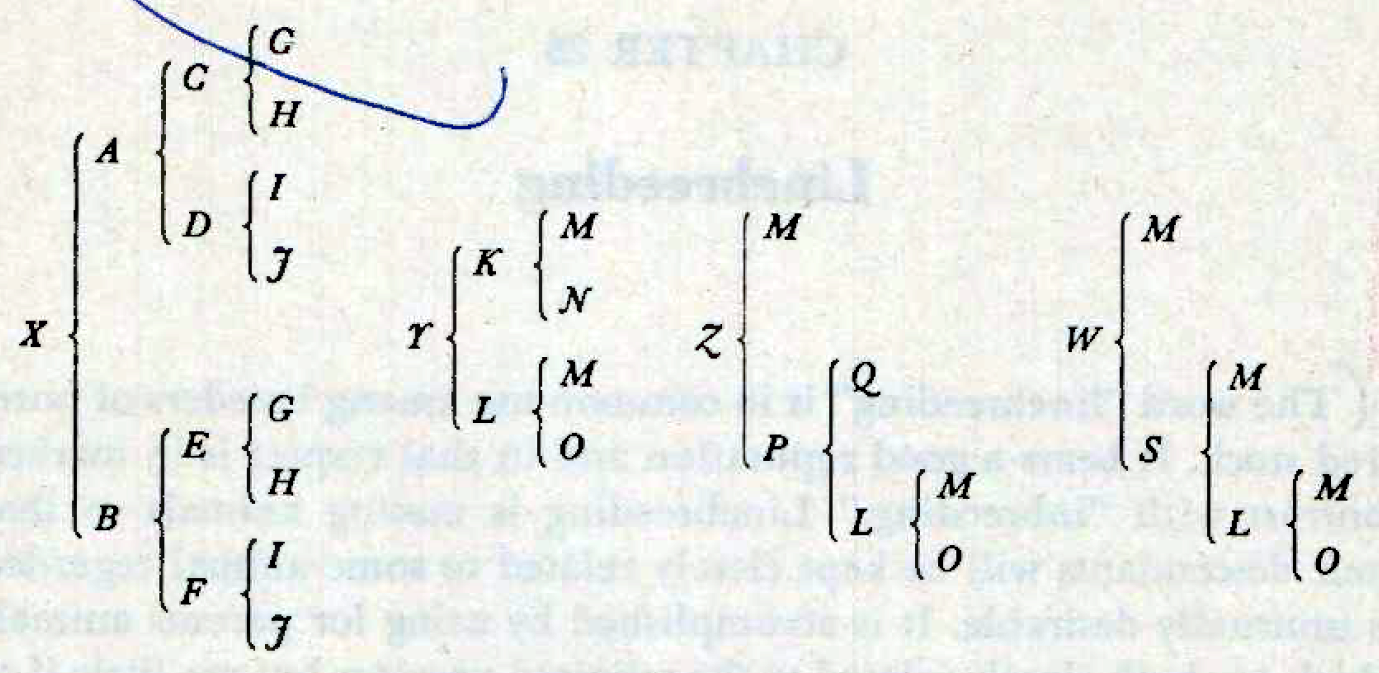
\includegraphics[width=\textwidth]{Page_300.png}
    \label{fig:Lush_Figure_Page_300}
\end{figure}

\section*{WHY LINEBREEDING IS PRACTICED}

Animals do not live long enough for the breeder to get all the sons
and daughters he wants from the best ones. Often an animal is old or
even dead before its real superiority is recognized . If its sons and
daughters are mated to unrelated individuals, the offspring will get
only about one -fourth of their inheritance from this outstanding grandparent.
If these in turn are mated to unrelated individuals, the influence
of the outstanding ancestor is again halved. Unless some form of
linebreeding is practiced, it is only a matter of three or four generations
until even the most outstanding animal's influence is so scattered and
diluted that no one descendant is very much like it. Linebreeding takes
advantage of the laws of probability as they affect Mendelian inheritance
to hold the expected amount of inheritance from an admired
ancestor at a nearly constant level instead of letting it be halved with
each generation, as would happen if all the matings were outbreeding.
Linebreeding provides, so to speak, a ratchet mechanism for holding
any gains already made by selection, while attempting to make further
gains.

Linebreeding also builds up homozygosity and prepotency within
the herd where it is practiced, just as other kinds of inbreeding do. It is
no more effective than other forms of inbreeding in this respect except
that, on account of the selection of the ancestors toward which the
inbreeding is directed, the \index{Homozygosis|}homozygosis produced by linebreeding is
more apt to be for desired traits than is the case with undirected
inbreeding. Linebreeding tends to separate the breed into distinct families,
each closely related to some admired ancestor, between which
effective selection can be practiced.

\section*{WHEN LINEBREEDING SHOULD BE PRACTICED}

The better the animals in a breeder's herd, the more reason he has
for linebreeding to them. The most vulnerable part in the linebreeding
program is whether the breeder is right when he decides which of the
animals recently used in his herd really were extraordinarily good ones.
If he can select the good from among the others with a high degree of
accuracy, linebreeding will be a powerful tool in his hands. If his judgment
about which animals were good is only fair, then linebreeding has
only a little advantage over other forms of inbreeding.

Those who can best afford to linebreed are breeders whose herds or
flocks are already distinctly superior to the general average of their
breed. If, by wise choice or lucky chance, such a breeder has used on
good dams a sire whose offspring turn out to be even better than their
dams, such a breeder ought to linebreed at once and strongly to this
sire while the animal is yet alive. If it is already dead when he discovers
how good it was, then he should hasten to linebreed to it while it still
has many sons and daughters by which such linebreeding can be accomplished.
While an animal is still living, the possibility of producing offspring
more closely related to it than any which yet exist remains open.
If a sire is thought good enough to make the risk worth taking, he can
be mated to his daughters and granddaughters generation after generation,
as seems to have been the intention of those who bred Blackcap
Empress (Figure~\ref{fig:Lush_Figure_30}). But after an animal dies the limit of relationship
to it which can be attained in future animals is only that of its closest
relatives then living. Even that is a limit only to be approached. If an
animal is dead by the time we realize how good it was and if there are
no living animals more closely related to it than 50 per cent, then there
is no possible way to produce animals more closely related to it than
that. If we have let its sons and daughters and full brothers and sisters
die before we wake up to its merit and there are left no living animals
more closely related to it than 25 per cent, then we cannot produce any
future animals more closely related to it than that -- hence the importance
of starting the linebreeding while there is time to do so effectively.
Figure~\ref{fig:Lush_Figure_39} shows a case where that seems to have been
planned definitely.

\begin{figure}
	\centering
    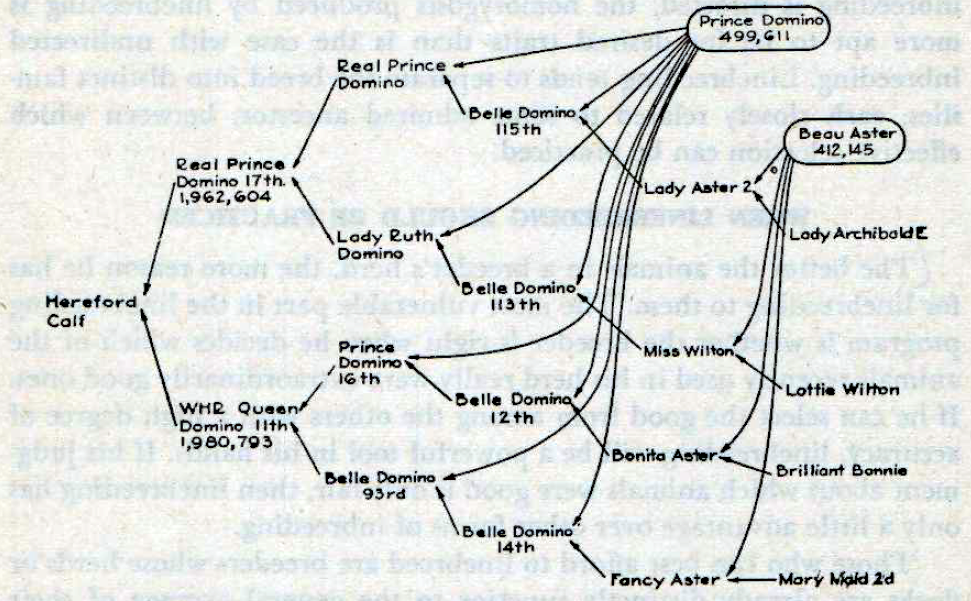
\includegraphics[width=\textwidth]{Figure_39.png}
    \caption{Long-continued and deliberate linebreeding to Prince Domino with a
			 very little linebreeding also to Beau Aster. Pedigrees like this do
			 not ``just happen.'' It took planning to get four different
			 grandparents with so nearly identical pedigrees and to bring them
			 together in this way without any secondary linebreeding.}
    \label{fig:Lush_Figure_39}
\end{figure}

\nowidow
It is an open question whether breeders with purebred herds of average
merit can afford to do much linebreeding. Certainly there are many
good animals in such herds and much good inheritance which stands
small chance of being kept together unless linebreeding is practiced. On
the other hand, if the initial merit of the herd was only average, one
must count on a certain amount of inbreeding degeneration which
might bring the average merit of the herd below the level of the breed.
The question at issue is whether the increased effectiveness of selection
possible under linebreeding will be more than enough to offset the
expected amount of inbreeding degeneration.

\index{Inbreeding!dangers of|(}
\index{Relationship|)}
Breeders of grades cannot often afford to linebreed. The inbreeding
risk involved is probably just a little greater for them than for the
breeder of purebreds on account of the slightly greater heterozygosis of
the grades. Even if a breeder of grades is successful at linebreeding, he
cannot sell at a premium the increased prepotency and uniformity
which would thus be put into his animals. He does not have the chance
to gain as much by successful linebreeding as breeders of purebreds do.
However, it sometimes happens that the breeder of grades uses a sire
whose offspring turn out to be so much better th:i.n their dams that the
inbreeding risk of using the sire on his own granddaughters or even on
his own daughters seems worth taking. It seems likely that there are
more breeders of grades who lose by failing to conserve a good sire than
there are who lose by getting too many of the usual bad results of
inbreeding while trying to linebreed to a good sire. For the breeders of
grades, the certain merit of the animal to which he might linebreed
needs to be further above the probable merit of the next sire which he
would otherwise use than is the case with the breeder of purebreds.

\index{Epistatic effects}
Linebreeding is especially needed where there is much epistasis.
Wherever a desired characteristic depends on a combination of genes
which individually have undesired effects, those gene combinations
tend to be scattered at each segregation. If inbreeding has made the
family homozygous for several of these genes, the whole combination
has more chance of being transmitted to enough of the offspring to
permit its becoming established in that family. If the form of inbreeding
used is linebreeding, with selection constantly directed toward keeping
the family closely related to animals which once showed that
desirable combination, the chances of recovering the whole combination
among the descendants are much better than if the descendants
were continually outbred to unrelated animals. Outbreeding would
increase the likelihood that this particular combination of genes would
be scattered into its constituent and individually useless parts. Linebreeding
is the only very promising way of securing desirable gene
combinations differing from the most frequent type of the breed by
much more than four or five gene substitutions, each of which is harmful
if made one at a time but beneficial if all can be made at once. That
is, linebreeding is the answer to the situation pictured in
Figures~\ref{fig:Lush_Figure_20} and \ref{fig:Lush_Figure_21}, in chapter
12, where it was pointed out that selection could carry a
population to the nearest peak of desirability but could not carry it to a
peak of higher desirability across an intervening valley which was more
than a few gene substitutions in width.
\index{Inbreeding!dangers of|)}

\section*{DANGERS OF LINEBREEDING}

The breeder may have the wrong ideal and be breeding toward a
type which has a lower sale value than some other type. Of course this
same danger exists in all other breeding systems. But, since linebreeding
is more effective in carrying the breeder toward his goal, it is more
important for a breeder practicing linebreeding to be sure of his goal
than for one who is breeding by individuality alone.

Linebreeding may be so intense that genes will become homozygous
more rapidly than the breeder can discard the undesired homozygotes.
The inbreeding may thus result in fixing in his herd some undesired
genes in spite of all the selecting he can do against them. Whether this
will happen depends not only on the inbreeding intensity but on the
merit of the stock with which he starts and on the skill which he exercises
in his selection, including such use as he makes of progeny tests,
pedigree estimates, etc. Then, too, a part of the success or failure will
be due to the chance inherent in Mendelian inheritance whereby one
individual from a particular mating may happen to be a better or worse
individual than would ever be produced again from that same mating.

There is no magic about the linebreeding process which will automatically
produce good results. If selection is not practiced, a breeder
will generally do better to avoid linebreeding altogether, since he would
thereby avoid the inbreeding effect. But a breeder starting with good
stock and directing the linebreeding toward the best of the recent ancestors
in his herd can effect more improvement by selection while holding
the improvement he already has than would be possible if he were continually
outbreeding.

\begin{figure}
	\centering
    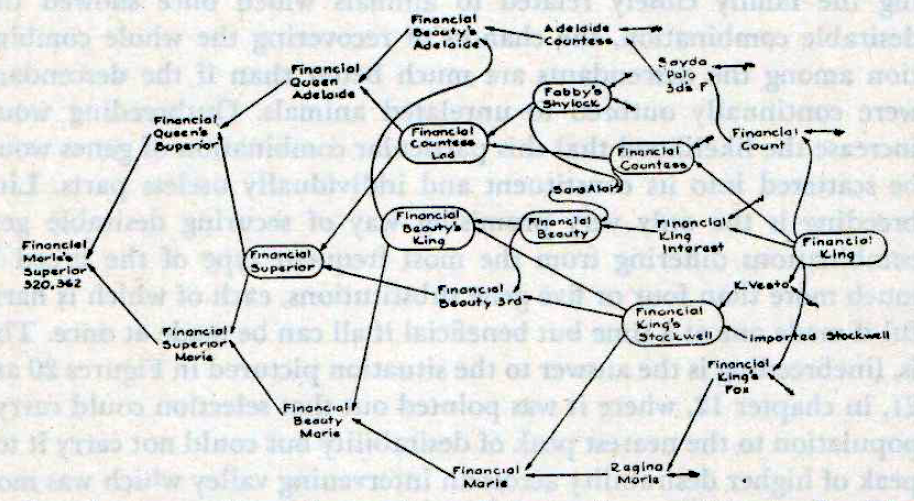
\includegraphics[width=\textwidth]{Figure_40.png}
    \caption{Long-continued linebreeding within the Financial King family of Jerseys.
			 Much of the linebreeding here is secondary and to recent animals such as
			 Financial Superior, Financial Countess Lad, and Financial Beauty's King.}
    \label{fig:Lush_Figure_40}
\end{figure}

If one wishes to linebreed purely to one animal, he must see to it
early that a large number of sons and daughters of that animal are
saved. Otherwise the time quickly comes when furth er linebreeding to
that ancestor also involves considerable linebreeding to some of its
descendants. Figures~\ref{fig:Lush_Figure_38}, \ref{fig:Lush_Figure_40},
and \ref{fig:Lush_Figure_41} show cases of that. There is no particular
lar reason why this secondary linebreeding should be avoided if the
animal toward which it is directed is an unusually good one. But, if the
herd is small and only one man is linebreeding to this line, there will be
only a few individuals in each generation. In some generations it will
happen that no one of those will be outstanding enough to justify linebreeding
to it. If the number of animals in this linebred strain or family
is very small, the breeder must either linebreed to some of those which
were not good enough to justify it, or else he will have to give up his
linebreeding plan and m.ake a distinct outcross. This is the intrinsic
danger of a permanent line breeding policy based on too small a herd. If
the herd is large enough, such secondary linebreeding can be avoided or
at least can be kept so small in amount in those generations when there
is no outstanding individual that it will be practically harmless. Hence,
a linebreeding plan which is to last more than two or three generations
without much risk requires the equivalent of a herd large enough to
justify keeping about three to five sires in use at all times.\footnote{These
figures are based on the $1/8M$ formula for loss of hetcrozygosis within
a closed group. (See Chap. 21.)} This might be one large herd; or several
breeders with small herds might co-operate in breeding toward the same line,
exchanging breeding stock with each other but rarely if ever introducing a
breeding animal from herds not in the group.

\begin{figure}
	\centering
    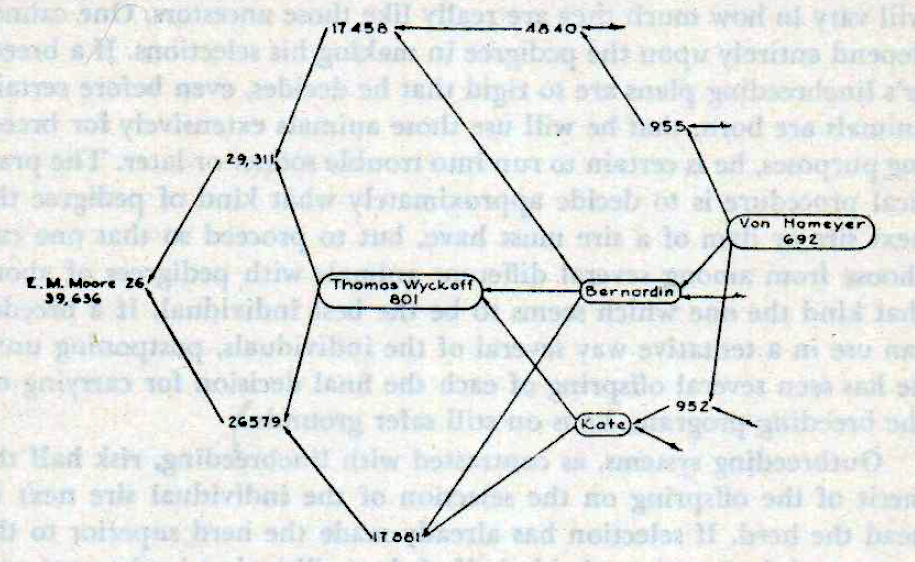
\includegraphics[width=\textwidth]{Figure_41.png}
    \caption{A Rambouillct pedigree in which one male is the center of the line breeding
			 in each generation.}
    \label{fig:Lush_Figure_41}
\end{figure}

\section*{GENETIC ASPECTS OF LINEBREEDING}
\index{Inbreeding|(}

Linebreeding, more than any other breeding system, combines selection
with inbreeding. In a certain sense, linebreeding is selection among
the ancestors rather than among living animals. Since many of the
ancestors being considered will have had several different offspring,
they arc to some extent proved sires and proved dams. The linebreeding
is, therefore, selecting from among progeny-tested\index{Progeny test} ancestors those
whose influence is to be preserved. This advantage is partly offset by the
fact that the individuals used to preserve the traits of their ancestors
will vary in how much they are really like those ancestors. One cannot
depend entirely upon the pedigree in making his selections. If a breeder's
linebreeding plans are so rigid that he decides, even before certain
animals are born, that he will use those animals extensively for breeding
purposes, he is certain to run into trouble sooner or later. The practical
procedure is to decide approximately what kind of pedigree the
next sire or dam of a sire must have, but to proceed so that one can
choose from among several different animals with pedigrees of about
that kind the one which seems to be the best individual. If a breeder
can use in a tentative way several of the individuals, postponing until
he has seen several offspring of each the final decision for carrying on
the breeding program, he is on still safer grounds.

\index{Outbreeding}
Outbreeding systems, as contrasted with linebreeding. risk half the
merit of the offspring on the selection of the individual sire next to
head the herd. If selection has already made the herd superior to the
average of the breed, probably half of that will be lost in the next generation
unless selection is again as effective as it was before. Every
breeder will occasionally make mistakes in his selections. The breeder
who continually practices outbreeding can therefore expect to have the
merit of his herd at times go far back toward the average of the breed.
One who wants to make and keep his herd far different from the average
of the breed to which it belongs must put some kind of a pedigree
barrier between it and the rest of the breed, so that the differences continually
being produced as successive sires are used will tend to accumulate
and not be halved with each successive sire. An analogy may make
that point clear. Water tends to seek its level. If there were no barriers
in the way, the level of the water in all the lakes of the world would
quickly seek the level of the ocean, just as the water in the rivers is
continually doing. The breeder who practices outbreeding is placing
no barriers, except his own skill at selecting, in the way of his herd's
tending toward the average level of the breed. The breeder who practices
linebreeding is to a considerable extent isolating his herd from
the rest of the breed, and its merit tends toward that of the isolated
group rather than toward that of the breed as a whole, just as the level
of the water in Lake Erie remains nearly constant but several hundred
feet above the level of the water in the ocean, even though water is
steadily flowing into it and out of it again.

\section*{SUMMARY}

Linebreeding is a form of inbreeding directed toward keeping the
offspring closely related to a highly admired ancestor. All inbreeding
not necessary for holding this relationship high is avoided as far as possible.
Hence, the intensity of the inbreeding is usually moderate in
linebreeding systems. Relationship to a chosen ancestor is the main
feature which distinguishes linebreeding from other forms of
inbreeding.

It is practiced to conserve the good traits of an outstanding sire or
dam among its descendants, increasing those descendants in numbers
without lessening their resemblance to this ancestor.

The more superior a breeder's herd or flock is to the average merit
of its breed the more reason he has to practice linebreeding to his very
best animals or to the very best of their recent ancestors.

The risk involved in linebreeding depends upon how much undesirable
inheritance is in the herd when the lincbreeding begins, upon
how skillful the breeder can be in his selections, how much use he can
make of progeny tests before he has to decide whether to use a sire
extensively, how large his herd is, and whether he must work alone . If
he can co-operate with several other breeders who are linebreeding to
closely related animals, he can get an occasional mild outcross from
them without disturbing his whole program.

Linebreeding is choosing which ancestors shall have their influence
conserved and spread through the whole herd and which ancestors shall
be allowed to diminish in importance with each generation until they
no longer have much effect.
\index{Inbreeding|)}
\index{Linebreeding|)}
\chapter{The Family Structure of Populations}
\label{cha:Lush_Chapter_24}
\index{Family differences|(}

Even in populations which are breeding entirely at random, an
individual does not have the same probability of being like every other
individual. Each is more closely related\index{Relationship} to some than to others. This
gives the population some kind of a family structure. Biological populations
are not as homogeneous as a population of balls or numbered
tickets in an urn, such as are often used to illustrate the elementary
laws of probability.

The definition of family always has in it something of the idea that
members of the same family are like each other and different from
members of other families. Yet usage varies widely as to the degree of
relationship which is meant. Sometimes family means a set of full sibs.
This is frequent in poultry breeding, but so restricted a definition is
uncommon in other animals where the number of full sibs is usually too
small for this to be very useful. In plants which can be self-fertilized,
family often means all the progeny of a single plant. It may mean a
more highly inbred group than that, but usually ``line'' is then used
rather than family. In animals which have long been linebred to a certain
individual, family may mean the whole group of individuals which
are linebred enough to be closely related to this individual and to each
other. An example is the Owl-Interest family of Jerseys.

In animals where little or no linebreeding has been practiced, family
is more likely to mean the descendants of a particular individual,
usually a purchased one (a ``foundation'' aimal [\textit{sic}]) or one thought to be
unusually good and with offspring well above average. Sometimes this
usage is carried to extremes, the family name being traced back only
through the female line (Shorthorns and Aberdeen-Angus) or only
through the male line (Herefords) to an ancestor so remote that, if there
has been no subsequent linebreeding, most of its descendants are little
if any more related to each other than they are to other animals of that
breed. Such usage is much like the transmission of family names in
man. There is little more reason to expect any real average difference
between Blackbirds and Ericas in Aberdeen-Angus than there is to
expect differences between the Smiths and the Wilsons in the United
States or between the Hansens and the Larsens in Denmark! The idea
of relationship between members of the same family becomes very dim
here, and family names tend to become artificial designations which
may be convenient but do not correspond to any biological reality.

Taxonomists use family in a special and definite sense to denote a
group which is intermediate between a genus and an order, as the cat
family (\textit{Felidae}), the deer family (\textit{Cervidae}), cattle
family (\textit{Bovidae}), etc.

We will consider first some of the less definite usages of family and
then the family as a basis for selection.

\section*{THE FAMILY --- A GROUP OF CLOSE RELATIVES}
\index{Family name|(}

When we say that an individual is from a good family, we usually
mean that the average merit of all its near relatives, regardless of whether
they are related through the sire or dam or bear the same family
name, is considerably above the breed average. This is the same sense in
which the term is often used in man when someone is said to be of ``a
good family'' or from ``a shiftless family.'' Family, in this sense of the
word, usually does not extend much farther among the collateral relatives
than to first cousins. Not often is anything implied about ancestors
farther back than the great grandparents, or about descendants much
more distant than grandsons and granddaughters. This use of family is
a practical application of relationship in estimating the heredity of an
individual from the appearance and performance of a considerable
number of its close relatives.

The family in this sense is somewhat indefinite, and one family
grades into another. For example, an individual's maternal uncles and
its paternal uncles are members of its family but the paternal uncles
need not belong to the family of the maternal uncles at all. In fact, no
two individuals would belong to exactly the same family unless they
were full sibs. The individual is at the center of its family with its relatives
clustered around it at various distances according to their relationship.
There is no accurate and simple formula for giving proper weight
to different relatives when averaging their good and bad qualities to
find the merit of the family, although of course the closest relatives are
the most important-unless there are strong environmental correlations
between them, as may sometimes be the case with maternal sibs. If the
family contains only a few members, chance can still play a large part
in giving one such family a good rating and another one a poor rating.

\section*{THE FAMILY NAME}

An Aberdeen-Angus cow is called an Erica if she traces through an
unbroken female line to the cow called Erica, regarded as the foundress
of the family. Technically she is still an Erica even if she does not trace
to Erica through any other line of her pedigree. In the Shorthorn and
Aberdeen-Angus breeds the family name is traced through the dams.
In the Hereford breed the family name is from the sire. In most dairy
breeds the family name comes from the dam, but in some both systems
prevail. The Holstein-Friesians have the De Kol family and the Pietertje
family which take their names from foundation cows, but the
Netherland family takes its name from the bull. In the Jersey breed
such families as Tormentor and Golden Lad are named after bulls; but
there are also such families as Coomassie, Fontaine, and Oxford named
after cows. Breeders of cattle and horses mention family more than do
breeders of sheep and swine.

This idea of family is a natural development in one-sire herds. A
breeder with several cows but only one bull will, of course, observe
many differences between his calves. Since all his calves in any one calf
crop are sired by one bull, it would be natural to assume, without even
realizing that he had done so, that all the differences between the calves
were due to differences in their dams. If when the successive calves from
the same cows are compared it is seen that there is a general tendency
for one cow to have good calves and another one to have mediocre
calves, it is natural for the breeder to group his animals in his own mind
in terms of their dams or grandams, as far back as he remembers those.
The inference that all the differences between the calves are due to differences
in their dams is, of course, unjustified, since the sire is never
entirely homozygous and some of the differences between the calves
will be due to difference in the inheritance they have received from him.
This tendency for the owners of small herds to think of families in
terms of female foundation animals is reversed in large herds where
several sires are maintained at all times. It is difficult for the breeder to
know all of his individuals closely in such herds and easy for him to
compare the calves by one sire with their contemporaries by other sires.
This naturally leads to a system of referring to the calves in terms of
their sires and grandsires instead of their dams. Perhaps this is responsible
for the fact that the Hereford breed, which is prevailingly bred in
large herds, tends to trace its family through the male line, whereas
breeds more commonly bred in small herds tend to trace the family
through the dam.

\index{Pedigrees, abbreviated|(}
When the system of tracing the family name through the dam is followed
far, it naturally leads to printing the pedigrees in the ``abbreviated''
form, a sample of which is shown herewith in the pedigree of the
noted Shorthorn bull, Rodney. Pedigrees in cattle breeds other than
the Shorthorn are now usually printed in the bracketed form which
gives information on all lines to the same number of generations.
Breeders of horses often use the abbreviated pedigrees. Formerly only
that part of the pedigree which appears in columns in this example was
shown. In recent years footnotes about the three most recent sires are
added, as in this case. Figure 42 shows the pedigree as it would appear
in bracketed form. The line drawn across the pedigree separates the
information which is contained in the footnotes from that which is
given in the columns.

\begin{figure}
	\centering
    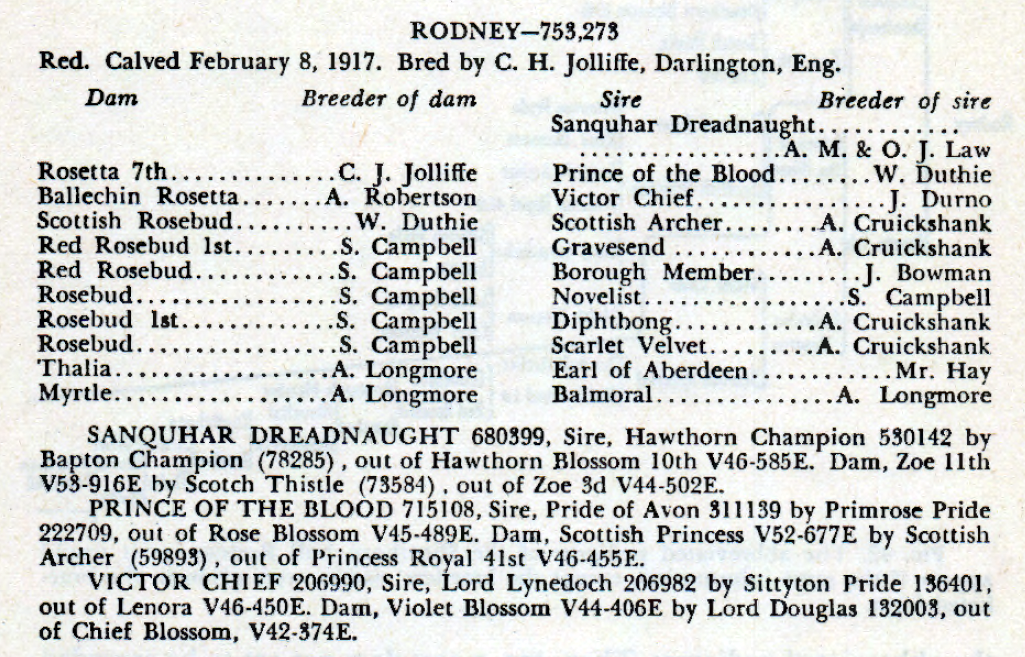
\includegraphics[width=\textwidth]{Page_311.png}
    \label{fig:Lush_Figure_Page_311}
\end{figure}

\nowidow
This abbreviated form of pedigree was fairly adequate when all of
the breeders were acquainted with the sires which were being used in
the prominent herds. There was no need to print the pedigree of the
sire, since each potential customer knew that. The customer would not
know all the females of the breed, so he did want to see the pedigrees of
the cows. When the breeds grew larger the time came when no one
knew all the sires; therefore, it became necessary to add these footnotes.
The abbreviated pedigrees emphasize remote ancestors beyond all usefulness.
For example, Rodney is called a member of the ``Rosebud family''
after the cow, Rosebud (by Scarlet Velvet), which was the first one
bred by S. Campbell, who developed this family. If there has been no
linebreeding to Rosebud in Rodney's pedigree, his relationship to her
will be \(\nicefrac{1}{2}^8\), which is about 0.4 per cent of his genes which probably
came from her. Rodney must have had literally tens of thousands of
contemporary relatives which had other family names but were more
closely related to him than was the cow from which his family name
comes.

The abbreviated pedigrees emphasize the names of the breeders.
The value of any pedigree is affected by the general reputation of the
herd in which the animal was bred. Something worth while is lost when
the name of the breeder is given a less prominent place than it has in
the abbreviated pedigrees. Then, too, a cow does not get to be regarded
as the foundress of a family on her own merits alone, but rather on the
high merit of many of her offspring. It is fairly safe to infer that Rosebud
1st and also Rosebud (by Novelist) were distinctly better individuals
than average or else Rosebud (by Scarlet Velvet) would not have
been regarded as the foundress of a family.

\begin{figure}
	\centering
    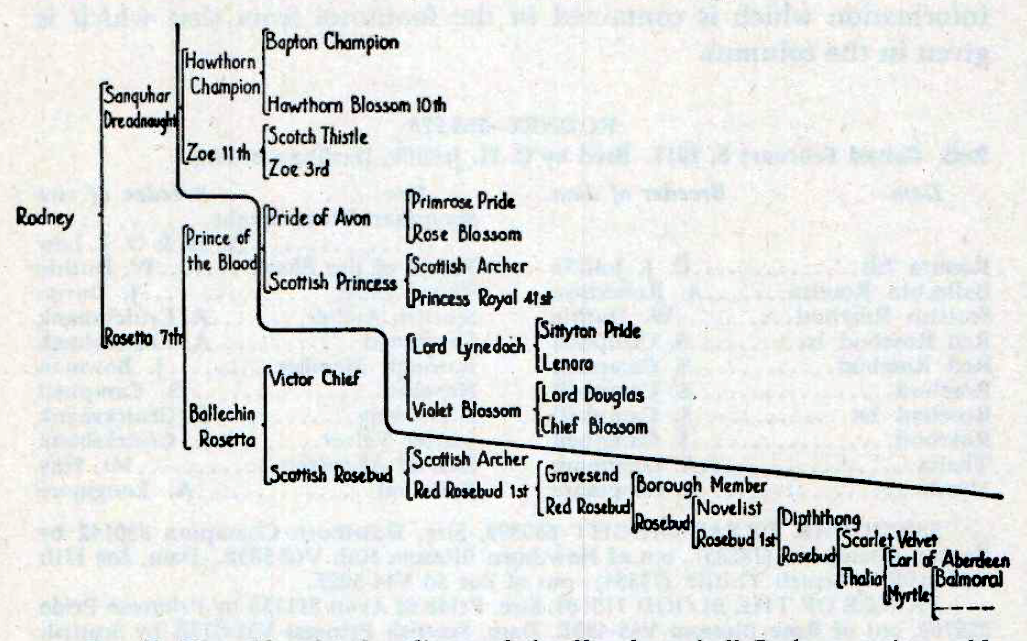
\includegraphics[width=\textwidth]{Figure_42.png}
    \caption{The abbreviated pedigree of the Shorthorn bu11 Rodney, as it would
			 appear if the same information, except the breeders' names, were
			 given in the bracketed form.}
    \label{fig:Lush_Figure_42}
\end{figure}

\index{Pedigrees, abbreviated|)}
The commercial importance of the family name is usually small,
unless perhaps in times of booms or pedigree speculation. It lends itself
well to speculation, particularly in breeds where the family name is
traced only through the female line. Even the best of cattle are none
too prolific, and a family can become famous and remain famous for
many years without a large number of females of that family ever existing
at any one time. If a strong demand for a family name can be created,
extreme speculation can easily result because the supply is limited.
Naturally such speculation is rare except when there is general prosperity
and prices for breeding stock have been rising for some time. The
most noted case of this kind was the speculation that went on in the
``pure'' Duchess Shorthorns in the 1870's. There have been several
periods of less extreme speculation in Aberdeen-Angus family names.
Yet in 21 Aberdeen-Angus sales, studied from this point of view from
1929 to 1938 in Iowa (unpublished), the only conclusion possible is that
practically no cash was really being paid for family name. However, this
was in a period of economic depression and perhaps this finding is not
significant. Four more sales from 1940 to 1942 when prices were rising
showed distinct price differences between families.

The family name has genetic importance when the animal which
gave its name to the family is still within three or four generations of
the animals concerned. In such a case the coefficient of relationship
between the animal and the foundation animal is still high enough to
mean that the two are apt to be alike in a noticeable proportion of
their genes.

Paying attention to maternal family names compels a certain
amount of added attention to the females in breeding selections. Some
breeders might be more careless about the dams if it were not for this
extra attention forced on them by the family system. The actual importance
of this may be slight.

The family name would have some genetic importance whenever
the general condition exists that breeders strive always to mate a cow of
one family to a bull of the same family; that is, to breed the family
``pure.'' If S. Campbell had always sought Rosebud bulls to mate to his
Rosebud cows, and if this had been continued to Rodney's time, Rodney
would have been kept very closely related (linebred) to the original
Rosebud cow. If that were a general practice among most breeders, it
would lead to steady linebreeding which might keep the foundation
animal important for many generations after its death. Where the family
system brings this about, it can be a powerful instrument in improving
the pure breeds, but this does not happen often. The cows in a small
herd may belong to a dozen families, but the same bull is usually mated
to all of them.
\index{Family name|)}

\section*{THE LINEBRED FAMILY}
\index{Linebreeding|(}

Sometimes ``family'' is used to designate a group which has been
partially separated from the rest of the breed for a long time in their
breeding and among which there has been considerable linebreeding.
Not often have such cases really been carried far enough to make the
family very distinct from the rest of the breed. Even a slight separation
of this kind has sometimes been the occasion for a large amount of
speculation in pedigrees. The most famous case is that of the ``pure''
Duchess Shorthorns, for which the pedigree speculation reached its
climax in 1876 in the New York Mills sale where one cow sold for
\$40,600. The ``pure Scotch'' Shorthorns are another example. In spite
of many bitter condemnations of the ``straight Scotch'' craze, the
straight Scotch almost entirely displaced the other beef Shorthorns in
the United States during the two decades preceding 1920. The ``straightbred''
or ``airtight'' Anxiety 4th Herefords may be a similar case in
which the final outcome is still in doubt. These straightbreds are a
group whose pedigrees in nearly every line go to daughters of North
Pole and to sons and daughters of Anxiety 4th. That is, they carry nearly
50 per cent of the blood of North Pole and Anxiety 4th combined.
Somewhat milder cases have happened in the Jersey breed in connection
with the Owl-Interests, the St. Lamberts, and Tormentors, and in
the Holstein-Friesians with the Homestead family.

The principles involved are just the same as those that have been
discussed under linebreeding. If the linebreeding has been carried far
enough to make the family really distinct from the rest of the breed,
then there is an important genetic basis for the family name. This kind
of a family is to some extent a breed within a breed.
\index{Linebreeding|)}

\section*{THE GENETIC DEFINITION OF FAMILY}
\index{Relationship|(}

The biological basis for treating a group as a family is the average
genetic likeness among members of the group. The best estimate of
genetic likeness where the actual genotypes are unknown is the coefficient
of relationship. This will usually give a reasonably true picture of
the average genetic likeness of family members where the base to which
relationship was computed is not many generations in the past.

As an example of this way of defining a family quantitatively, we
might choose to consider each set of full sibs in a random breeding
population as a family. For comparison with other kinds of families
we can define this kind as a group which are related to each other 50
per cent. If all the offspring of each male are to be considered as a family,
that kind of a family can be defined as a group related 25 per cent to
each other.\footnote{Although such a family will not be entirely homogeneous
if some of them are full sibs to each other, this will not increase the average
relationship much if there are more than three or four different sets of such
full sibs or if the number in each such set is small. For example, if the
progeny of a boar consist of four litters of five pigs each and we call this a
family, it will not of course be a perfectly homogeneous family but will be
one large family with four branches or subfamilies. The average relationship
of each pig to the other 19 will be an average of 4 full sib and 15 half sib
relationships or about 110 per cent. If the progeny of a bull are five pairs
of full sisters, the average relationship within the group of 10 will be an
average of 1 full sib and 8 half sib relationships or 28 per cent.} We can
compare the importance we should attach to family when making selections in
the two cases by using alternately .50 and .25 for \textit{r} in the formulas
which are in the next few pages. If all the grandsons and granddaughters of
a male are to be considered as a family, we can define this family as a group
which are related to each other 6\nicefrac{1}{4} per cent, plus a little
more from the fact that some of them will be sibs or cousins through more
than one grandparent. When family is thus defined quantitatively, it is easy
to see why the practical usefulness of family groupings becomes so small
when the group members are related only through ancestors as distant as
grandparents.

The observed family resemblance may be expressed either in tenns
of the correlation between members of the same family or in terms of
how much smaller the differences between members of the same family
are than the differences between members of different families. The
formula which relates the two is simply that the correlation between
members of the same family equals $\dfrac{V - B}{V}$ where \textit{V}
is the variance between individuals which belong to different families
and \textit{B} is the variance between individuals which belong to the
same family. $V - B$ is the variance caused by things which are alike
for all members of each family but may vary from one family to another.
$V - B$ might be wholly genetic in some cases but is likely also to
include some differences caused by common environment for family mates,
or by epistasis, or dominance.

The formulas showing quantitatively the advantages and disadvantages
of selection on a family basis are rather complex but they arc given
in the following sections because they are important guides for
estimating whether a plan for selecting on a family basis is likely to
increase progress sufficiently to be worth its costs.

\section*{CONDITIONS AFFECTING PROGRESS WHEN CHOOSING BETWEEN FAMILIES}
\index{Selection!on the family basis|(}

The formulas for comparing individual and family selection, when
the same percentage of the population must be culled in either case,
are expressed as follows for convenience:
\vspace{-0.2cm}
\begin{table}[h]
	\centering
	\begin{tabular}{R{1cm}L{11cm}}
		Let~$G$ & = the additively genetic variance between individuals. \\
		$E$ & = all other variance (largely environmental in most cases) which is random\\
			& with respect to family. \\
		$C$ & = the variance caused by whatever fraction of the environmental,\\
			& epistatic, and dominance deviations are alike for members of the\\
			& same family, but vary from one family to another. \\
		$r$ & = genetic relationship between members of the same family. \\
		$t$ & = phenotypic or observed correlation between members of same
family $=$ \\
			& $\dfrac{rG + C}{G + C + E}$. \\
		$n$ & = number of individuals in each family.
	\end{tabular}
\end{table}
\vspace{-0.6cm}
\begin{table}[h]
	\centering
	\begin{tabular}{R{1cm}L{11cm}}
	Then: & Variance between individuals from different families \(= E + G + C\) \\
		  & Variance between members of the same family \(= E + (1 - r)G\). \\
		  & Variance between actual family averages $=$ \\
		  & \hspace{2.5em}\(rG + C + \dfrac{1 - r)G}{n} + \dfrac{E}{n}\).
	\end{tabular}
\end{table}
\vspace{-0.2cm}

Having large numbers in the family permits the environmental differences
(\textit{E}) and the genetic differences between members of the same
family --- the $1 - r$ fraction of \textit{G} --- to cancel each other, so that the actually
observed differences between family averages tend toward $rG + C$,
which will be almost wholly genetic if \textit{C} is very small. When \textit{n} is small
a considerable part of the differences between the actually observed
averages of various families may still be due to the $E/n$ term which is
environmental and misleading.

The larger \textit{r} is, the more of the genetic variance (\textit{G}) will be between
families instead of within families. This will permit the family averages
to be farther apart, so that one can reach farther when selecting
between families when \textit{r} is large than when it is small. Also any
increases in \textit{r} will make a larger fraction of the observed differences
between family averages genetic, so that one selecting between family
averages will actually get a larger fraction of what he reaches for. To
have \textit{r} large is an important prerequisite for selection between families
to be very useful.
\index{Relationship|)}

When \textit{C} is large the heritability of differences between family averages
will be low, since that heritability tends toward $\dfrac{rG}{rG + C}$ as \textit{n}
becomes indefinitely large. Hence, with \textit{C} large many of the differences
between family averages will not be genetic, many mistakes will be
made in selecting between families, and only a small fraction of what is
reached for in family selection will actually be gained in the merit of
the offspring. The deceiving effects of \textit{C} do not diminish with increases
in \textit{n} as those of \textit{E} do. In the mammals, \textit{C} is especially
likely to be important when the family consists of maternal sibs.\footnote{Environmental
correlations between full sibs are also prominent in data on
man, especially in data pertaining to mental and social traits. Man's long infancy and
childhood and the wide differences from home to home in cultural environments and
parental precepts and examples give an unusual opportunity for such correlations
to develop in characteristics which are susceptible to much modification by such
influences.} \textit{C} is likely to be large
also in birds which hatch and brood their own young. Even in birds
hatched in incubators and reared apart from their dams, certain initial
environmental differences caused by the size of the egg may not be
wholly equalized before the birds are adult. In data collected from
many different farms, \textit{C} is often troublesomely large because environments
vary considerably from farm to farm, and in most cases each family
will have been raised wholly on one farm. In carefully planned
breeding experiments every effort will be made to reduce \textit{C} to zero by
controlling or randomizing the environment with respect to families.
Often that can be fairly well achieved for all of \textit{C} except the part due to
maternal environment and the part due to weather and to changes in
general environment from year to year in cases where the families are
not contemporary. But breeders when purchasing animals usually must
compare families kept in different herds. Then the best they can do to
eliminate \textit{C} is to observe the conditions under which each family is kept
and make allowances for the differences which they think these conditions
produced between families.

\section*{FAMILY SELECTION COMPARED WITH INDIVIDUAL SELECTION}

For clarity we will first consider what family selection would accomplish
if it were practiced by itself without any attention to individuality.
Figure~\ref{fig:Lush_Figure_43} will illustrate the difference between family selection
alone and selection on an individual basis. The data are 180-day weights
of four pigs in each of four litters. One-fourth are to be saved for breeding
purposes, and selection is for the heaviest weights. If selection is
wholly on a family (litter) basis, the selected pigs will be all four of
those in family 2, since that family has the highest average weight. Pig
\textit{E}, which has a low weight, will be selected along with the other three
because it is in the family with the high average. If selection is wholly
on an individual basis, pigs \textit{D}, \textit{G}, \textit{H}, and \textit{L},
will be selected regardless
of the merits of their sibs. If the method of selection is some compromise
which gives attention to family averages as well as to individual
merit, pigs \textit{F} and \textit{P} might possibly be saved instead of
pigs \textit{D} and \textit{L}.

Two things about this situation must be emphasized. First, one cannot
pay attention both to family apd to individuality without compromising
on both. Almost never will it happen that all members of the
family which has the highest average will be individually superior to all
members of the other families. One must compromise on one thing or
the other when deciding what to do with good individuals (like \textit{D} and
\textit{L}) from mediocre or poor families and with mediocre or poor individuals
(like \textit{F} and \textit{E}) from a good family. Second, some of the same animals
will be saved, no matter which method or compromise is used. The family
with the highest average must contain more than a fair share of individuals
which are above average. \textit{G} and \textit{H} illustrate this. Purely
individual selection does some of the same things which purely family
selection would do. If either method is \textit{absolutely} ineffective, the other
will be also. The contrast between them is between two methods both of
which will produce some improvement, if either of them will produce
any, but which will not, except by coincidence, produce exactly the
same amount of improvement per generation.

\begin{figure}
	\centering
    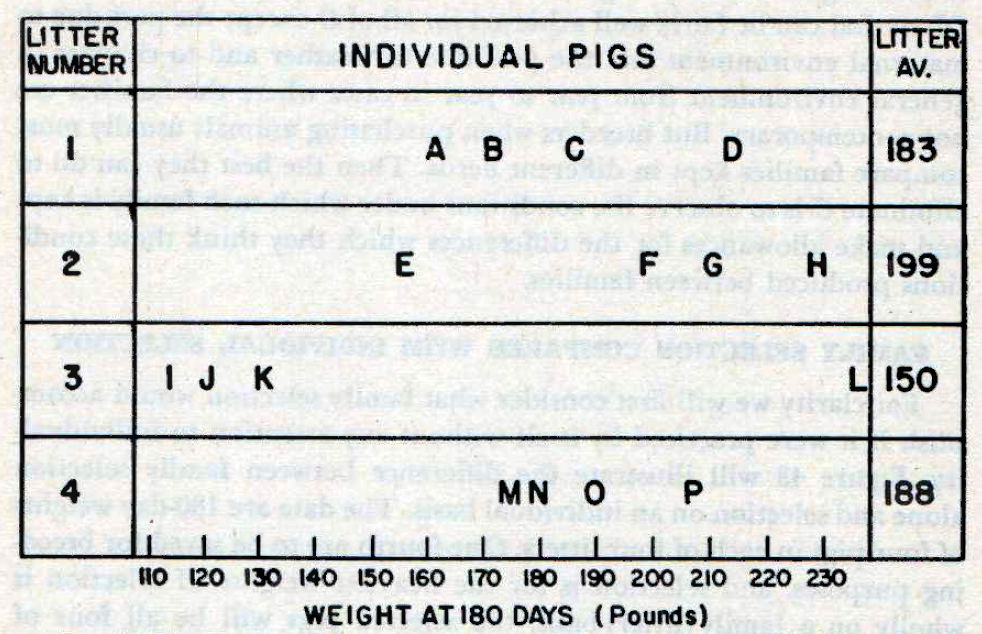
\includegraphics[width=\textwidth]{Figure_43.png}
    \caption{Distribution of some pig weights by litters to illustrate family and individual
			 selection. Each pig is designated by a letter located vertically according to its
			 litter and horizontally according to the pig's weight.}
    \label{fig:Lush_Figure_43}
\end{figure}

The increase in the population mean each generation under purely
family selection is expected to be the following fraction of the increase
to be expected under purely individual selection: \(\dfrac{1 + (n - 1)r}{\sqrt{n[1 + (n - 1)t]}}\).

Although this formula is complex, it can be seen that family selection
is most likely to be superior when \textit{r} is large and \textit{t} is small. Differences
in \textit{n} do not affect the ratio very much unless \textit{t} is extremely small
and \textit{r} is large. In that case high values of \textit{n} increase the effectiveness of
family selection markedly. If \textit{t} is nearly equal to \textit{r}, family selection can not
equal individual selection in effectiveness, even when \textit{r} and \textit{n} are
large.

\nowidow
If purely family selection is to produce improvement \textit{x} times as
rapid as would be produced by individual selection, then \textit{r} must equal
\(\dfrac{x\sqrt{n[1 + (n - 1)t]} - 1}{n - 1}\). For \textit{x} to be 1.0 when families
consist of 5, \textit{r} would have to be:

\begin{gather*}
.41 \text{ if } t \text{ is } .1 \\
.50 \text{ `` `` `` } .2 \\
.58 \text{ `` `` `` } .3 \\
.65 \text{ `` `` `` } .4 \\
etc.
\end{gather*}

If \textit{n} is as large as 25, the corresponding values of \textit{r} necessary
for \textit{x} to be l.O would be only a little lower, namely: .34, .46, .56, .64,
etc. In short, if family selection is to be much more effective than individual
selection, \textit{r} must be considerably larger than \textit{t}. Increases in
\textit{n} do not lower the requirements for \textit{r} much unless \textit{t} is very small.

Because \textit{t} equals $\dfrac{rG + C}{G + C + E}$, it is necessary for
\textit{C} to be nearly zero and \textit{E} to be much larger than \textit{G}
if \textit{r} is to be much larger than \textit{t}. When heritability is low
(\textit{G} is small, compared with $E + C$) neither
individual selection nor family selection will make rapid progress, but
family selection can then be considerably more effective than individual
selection if \textit{C} is zero or nearly so. Among important characteristics for
which \textit{E} is likely to be very large and \textit{C} may be small, are such complex
things as fertility, vitality, longevity, disease resistance in general,\footnote{Individual 
differences in resistance to some specific diseases may be rather highly genetic.} and
probably growth rate so far as that does not depend mainly on dimensions
of bones.

\section*{SUPPLEMENTING INDIVIDUAL SELECTION WITH FAMILY SELECTION}

It is sensible of course to use both the family average and the individual's
own characteristics in selecting, compromising somewhat on
each in order to make faster progress than could be made by using
either alone. The progress per generation which will be achieved under
the optimum combination of individual and family selection will be
the following fraction of what would be achieved by selection on individuality
alone:

\[ \sqrt{1 + \frac{(n - 1)(r - t)^2}{(1 - t)[1 + (n - 1)t]}} \]

The most important thing in determining how large this ratio will
be is the term, $r - t$, which measures how much more the members of
the same family are like each other genetically than they are outwardly.
When $t = r$, nothing at all is gained by paying attention to the family
average. The larger the difference between \textit{r} and \textit{t} the more there is to
gain by paying some attention to family. Even when \textit{t} exceeds \textit{r}, something
is to be gained from considering the family average, but in this
case the attention given to the family average is negative; i.e., the individual
is judged partly by its own merit and partly by how much it
deviates from its family average, instead of being given some credit if
the average merit of its family is high and being penalized if it is from a
poor family.

The numerical values in Table~\ref{tbl:Lush_Table_18} for some selected conditions may
make it easier to see what circumstances lead to much gain from paying
attention to family. The basic formula is that if paying attention both
to the individual and also to its family average is to make progress $1 + y$
times as rapid as if selection were on individuality alone, $r - t$ must
equal

\[ \frac{y(2 + y)(1 - t)[1 + (n - 1)t]}{n - 1} \]

\noindent
For progress to be made 20 per cent faster by considering the family
average requires the difference between \textit{r} and \textit{t} to be 1.45 times as large
as is necessary to increase progress by 10 per cent. If progress is to be
30 per cent faster, the difference between \textit{r} and \textit{t} will need to be 1.81
times as large; for 40 per cent it will need to be 2.14 times; for 50 per
cent 2.23 times is required; etc.

\begin{table}[htbp]
	\centering
	\caption{\textsc{Genetic Relationships Necessary if Paying Attention Also to Family is to
Iicrease the Rate of Improvement by 10 per Cent or by 100 per Cent}}
	\label{tbl:Lush_Table_18}
	\begin{tabular}{C{2cm}||C{2.25cm}|C{2.25cm}|C{2.25cm}|C{2.25cm}}
		\hline
		\hline
		 							& \multicolumn{2}{C{4.5cm}|}{For Progress to Be 10 per Cent
Faster (y = .1)}	& \multicolumn{2}{C{4.5cm}}{For Progress to Be Twice as Fast (y = 1.0)} \\
		\cline{2-5}
		t		& When $n = 5$ $r$~must $=$	& When $n = 25$ $r$~must $=$	& When $n = 5$ $r$~must $=$	& When $n = 25$ $r$~must $=$ \\
		\hline
		.01	& .27	& .11	& .89			& .40 \\
		.05	& .29	& .19	& .97			& .56 \\
		.10	& .36	& .26	& Impossible	& .72 \\
		.20	& .47	& .40 	& "				& .96 \\
		.30	& .58	& .52	& "				& Impossible \\
		.40	& .69	& .64	& "				& " \\
		.50	& .78	& .74	& "				& " \\
		.60	& .87	& .83	& "				& " \\
		\hline
	\end{tabular}
\end{table}

Since \textit{r} cannot exceed 1.0, extremely large gains from paying attention
to the family average are possible only when \textit{t} is very small. Also \textit{n}
must be large, but this of itself will not help much unless \textit{t} is so small
that $(r - t)^2$ is far larger than $t(1 - t)$. This marks out the domain in
which family selection is most useful, for \textit{t} can be small only when heritability
is low and when other causes (\textit{C}) for family members resembling
bling each other are zero or very nearly so. Then if \textit{r} and \textit{n} can both be
made large, selection on the family basis can increase progress very
much.

Family selection and individual selection are mainly supplementary
procedures rather than competitive ones, individual selection doing
nearly all that the two together could do when heritability is high but
declining in effectiveness in direct proportion to the decline in heritability,
while family selection helps little when heritability is high but
increases in relative effectiveness as heritability of individual differences
declines. Thus, in framing efficient breeding plans, attention should
gradually shift from individual selection to emphasis on family selection
more and more as one turns from highly hereditary to less and
less hereditary characteristics.

\section*{OPTIMUM ATTENTION TO PAY TO FAMILY AVERAGE AND TO INDIVIDUAL MERIT}

For the maximum rate of improvement, each bit of merit or defect
in the family average should receive $\dfrac{n}{1 + (n - 1)t} \cdot \dfrac{r - t}{1 - r}$
times as much attention as the same absolute amount of merit or defect in the
individual's own characteristic. This ratio is large when \textit{r} is large, \textit{t} is
small, and \textit{n} is large, although the latter doesn't make much difference
unless \textit{t} is small. This ratio goes to zero when $r = t$ and takes negative
values when \textit{t} exceeds \textit{r}. For \textit{t} to exceed \textit{r}
means that \textit{C} is large and that each family average is being shoved up
or down by circumstances other than the average breeding value of that family.
That the fraction then is negative merely indicates that it is then more
accurate to judge the individual partly by its deviation from its family average,
as an automatic way of correcting partly for the nongenetic circumstances included
in \textit{C}. The deviation of the individual from its family average is
composed of variation coming from \textit{E} and from $(1 - r)G$ and does not
include the \textit{C} term. To judge the animal entirely by its deviation from
its family average would open the door to large errors from \textit{E} and
would forego opportunity to select for differences caused by \textit{rG}. Hence
the optimum combination of attention to family and to individuality is
a compromise aimed at some discounting of \textit{C}, some use of \textit{rG} as well as
$(1 - r)G$, and some reduction of \textit{E} by \textit{n}.

The conditions when attention to the family average should turn
negative may actually be reached in data where \textit{r} is low and \textit{C} is large,
as in dairy production records used in proving bulls which have been
kept and used in different herds. Also characteristics markedly influenced
by prenatal or pre-weaning differences in environment are likely
to have a large \textit{C} between litter mates. For such characteristics in pigs,
full sibs which are not litter mates or even paternal half sibs may
deserve more attention than litter mates.
\index{Selection!on the family basis|)}

\section*{INBREEDING AND THE FAMILY STRUCTURE OF POPULATIONS}
\index{Inbreeding|(}
\index{Variation!increased by inbreeding|(}

Inbreeding helps in several ways to make family selection more
effective. First it increases \textit{G} to $1 + F$ times what it was in the
foundation population.\footnote{The increase will generally be somewhat more
than this if there is much dominance or epistasis. But \textit{G} may actually
decline if enough of the poorest families are culled while the inbreeding
is being done.} This also helps mass selection by increasing the standard
deviation a little and thus making a larger selection differential
possible. A more important effect is that it increases heritability, and
thereby a larger fraction of the selection differential is actually gained
in the offspring. The gain had by increasing \textit{G} is rather quickly
exhausted when the poorer families are culled. To renew it the remaining
families must be intercrossed and distinct families formed again by
inbreeding these crosses. It is therefore a gain which cannot be harvested
in every generation.

In the second place, inbreeding is the only way to make \textit{r} much
larger than .31 in large families of the less prolific animals, or larger
than .50 in families of animals like pigs and chickens. As a numerical
example of how rapidly inbreeding will increase \textit{r}, the full sibs in the
first inbred generation of full brother-sister inbreeding are related 60
per cent, in the second generation 74 per cent, and in the third generation
79 per cent -- compared with 50 per cent where there is no inbreeding.
The \textit{r} between full sibs equals $50\left[1 + \dfrac{F + F'}{1 + F}\right]$ per cent,
\textit{F} being the inbreeding of sibs and $F'$ the inbreeding of their parents. This
shows vividly for full sibs how closely the increase in \textit{r} beyond 50 per
cent depends on the intensity of inbreeding. In continuous half sib
inbreeding -- one sire in a large herd closed to outside blood -- half sibs
in the first inbred generation are related 39 per cent, in the second generation
50 per cent, and in the third generation 58 per cent. How
rapidly inbreeding will increase the genetic relationship between
half sibs may be seen from the fact that this relationship equals
$25\left[1 + \dfrac{5F + F'}{1 + F}\right]$ per cent, provided the three parents
are equally inbred and equally related to each other.

Even one or two generations of rather mild inbreeding can raise \textit{r}
enough to increase greatly the proper amount of attention to pay to the
family average for the most effective selection, especially if the characteristic
is only slightly hereditary, since then the accompanying increase
in \textit{t} would be far less than the increase in \textit{r}. This may be a very practical
procedure under many circumstances, since the risk of inbreeding
degeneration would not be large, it would take only a generation or
two to produce this much inbreeding, and therefore a selection between
families could be made every second or third generation. To carry
inbreeding to higher levels before making the selections between families
would make both \textit{r} and \textit{G} larger and would make selection between
families more effective in the generation in which it was practiced, but
would involve more inbreeding risk and would require more generations
for each cycle of inbreeding, selection, and re-crossing the selected
families. Therefore, it might make less net progress per generation
than the shorter cycles with the milder inbreeding. Not all of these relations
have been explored yet, but it appears\footnote{Dickerson, G. E., 1942,
Experimental design for testing inbred lines of swine,
\textit{Jour. of An. Sci.}, Vol. 1.} that not much is to be
gained by increasing the inbreeding much farther than 30 per cent
before selecting between the lines, unless epistatic interactions are
highly important.

A third way in which inbreeding can make family selection more
effective is that it permits high values of \textit{r} without necessarily having
high values of \textit{C} in those characteristics where maternal environmental
influences are strong or where contemporaneity carries with it some
strong environmental correlations. Without inbreeding it is difficult to
get families which have \textit{r} much larger. than .31 and yet are not maternal
sibs, and impossible to get such families with \textit{r} as large as .38. Yet in the
second inbred generation of continuous half-sib inbreeding, the members
of the same family will already be related to each other 50 per cent
and in the third generation 58 per cent, although they are not from the
same dams.

The close relation between intensity of inbreeding and distinctness
of families is shown by the speed with which, in a population inbred
steadily without selection, the genetic variance tends to be shifted from
variance within families, $(1 - r)G$, to variance between families, $rG$. In
regular full-sib inbreeding, $rG$ equals $(1 - r)G$ before the inbreeding
begins, is 1.5 times as large in the first inbred generation, 2.7 times as
large in the second, 3.8 times as large in the third, etc. In regular halfsib
inbreeding the corresponding ratios are .33 before the inbreeding
begins, .64 in the first inbred generation, 1.00 in the second, 1.40 in the
third, 1.86 in the fourth, etc. The general formulas are that $rG$ equals
$2/G_0$ and $(1 -r)G = (1 + F - 2f)G_0$ where \textit{F} is the inbreeding of the
animals concerned, \textit{f} is the average inbreeding of the offspring which
would be produced by mating members of the same family together,
and $G_0$ is what \textit{G} was in the foundation generation to which the
inbreeding and relationship coefficients are traced. The ratio of the
genetic variance between unrelated lines to that within lines thus
becomes $\dfrac{2f}{1 + F - 2f}$.

This forming of families between which selection could then be
more highly effective may have been the major part which inbreeding
played in the development of hybrid corn. The inbreeding was carried
so far that \textit{r} was nearly 1.0 and \textit{G} was nearly doubled. In that condition
the differences between lines were almost wholly genetic (except for
whatever there was in \textit{C}), and selection between them for their combining
power could be more effective than ever before. However, this is not
the whole story, for the inbreeding also aided greatly in purging the
the lines of rare and undesirable recessives, and was almost the only
means for isolating and comparing epistatic combinations. These effects
may have been very important, too.
\index{Inbreeding|)}
\index{Variation!increased by inbreeding|)}

\section*{FAMILY DISTINCTNESS AS AFFECTED BY DOMINANCE AND EPISTASIS}

\index{Epistatic effects|(}
\index{Dominance}In random breeding populations most of the effects of dominance
are included in the \textit{E}term, but when members of a family are related
through both parents of each, there is some correlation between their
dominance deviations. This contributes a little to the \textit{C} term in such
families. If a population is being inbred, the heterozygotes become scarcer
and the variance caused by dominance deviations tends to disappear,
part of it going to join the increases in the \textit{G} term.\footnote{This is
curvilinear, and there are certain special but uncommon combination
of circumstances under which the variance due to dominance deviations would
increase a bit in the early stages of inbreeding, before beginning to decline.} Thus the
general effect of dominance is to make the \textit{E} term distinctly larger and
the \textit{C} term a little larger than if there were no dominance. It makes the
effectiveness of family selection increase with advancing inbreeding a
little more than the preceding formulas indicate.

Variance due to epistatic gene interactions likewise goes mostly into
the \textit{E} term when inbreeding is zero, but the epistatic deviations of family
members are correlated, and this contributes something to the \textit{C}
term. As inbreeding gets more intense, the correlations between epistatic
deviations of members of the same family rise with \textit{r} at an ever increasing
rate. This increases \textit{C}, but also some of what were epistatic
deviations in a random-breeding population can be gathered into the
additive scheme in partially inbred populations. This increases \textit{G} at the
expense of \textit{E} and perhaps of \textit{C}. The net result is that family
differences and distinctness become even more pronounced with increasing
inbreeding than was indicated in the preceding formulas. Presumably
this makes family selection more advantageous than the preceding formulas
indicate.
\index{Epistatic effects|)}

\section*{RELATED FAMILIES}
\index{Relationship|(}

In actual populations the families are not wholly unrelated to each
other. Instead each family is related to others -- to a few closely, to some
less closely, and to most scarcely at all unless the relationship is relative
to a basis farther back than the time when this population first diverged
from other populations. The family structure of a population is somewhat
like a fishing net in which each knot is rather close to a few others
but distant from most.

Since each individual has two parents but the number of its offspring
can vary from zero to many, the network of descent as traced
backward will necessarily be more regular than when traced forward. If
there has been some degree of inbreeding and separation of the population
into small and partially isolated subgroups between which there
is little inbreeding, the irregularity of the family structure of the population
may become extreme. It is somewhat like an irregularly torn and
tangled net, some clumps of strands being heavily intertangled with
each other but swinging almost free from adjacent strands and only
remotely connected with the rest of the net. Some of the subgroups
themselves at a later date may be subdivided still further into partially
non-interbreeding groups. Thus arise families within families.

When selection is to be practiced between such related families, the
effective \textit{r} between members of the same family is approximately
$\dfrac{r_2 - r_1}{1 - r_1}$ where $r_2$ is the relationship within the
family, and $r_1$ is the relationship of the two families to each other.
For example, suppose two families are related 20 per cent to each other,
but the relationship within families is 50 per cent. Then, for selecting
between two individuals each belonging to one of these families, the
\textit{r} in the preceding formulas for determining how much attention
to pay to the family average is approximately $\dfrac{.5 - .2}{1 - .2}$,
or about 38 per cent. The practical consequence is that when
separate families are built from a common and closely related foundation
stock, the inbreeding needs to be pushed further for selection
between families to reach a given effectiveness than if each had been
started from an unrelated stock. When selecting between individuals
from related families, the family averages should receive less attention
than when selecting between individuals from unrelated families. The
common sense of this is obvious when one considers the extreme case of
selecting between full sibs. The family average is useless for helping discriminate
between them, since it is exactly the same for both. In selecting
between two half sibs the family averages of each are partly
determined by the common parent. To that extent the family averages
are less helpful in indicating which of the two has the higher breeding
value. The discussion here and formula for effective \textit{r} merely generalize
the principle of this and extend it to less obvious cases.
\index{Relationship|)}

\section*{SUMMARY}

The term ``family'' in animal breeding implies a group of animals
related to each other, but usage varies widely as to how close that relationship
must be before two individuals are considered as members of
the same family. Often the definition of family is vague and variable,
even in a single discussion.

Family often signifies a name which is handed down, perhaps for
many generations, usually through the female line but occasionally
through the male line. As such it has no more real significance than
human family names do. However, it lends itself to speculation in boom
times and has sometimes played a part in making some purebred individuals
sell for higher prices than others of the same breed. It may help
emphasize the breeder's name. It may make selection of females a bit
more strict than would otherwise be the case.

If females are consistently mated to males of the same family as their
own, such linebreeding tends to make and keep families distinct from
each other. If the linebreeding is continued long or becomes intense,
such a linebred family tends to become a breed within a breed. Such
distinct families within pure breeds have been formed only occasionally.

The family has a measurable genetic basis and practical usefulness
when it is defined as a group with an average genetic relationship,
\textit{r}, to each other. Attention to family is most helpful when
\textit{r} is large and the observed resemblance of family members,
\textit{t}, is low. Each bit of merit or defect in the family average
should receive $\dfrac{r - t}{1 - r} \cdot \dfrac{n}{1 + (n - 1)t}$
times as much attention as the same amount of merit or defect in the
individual.

The family should be given negative attention when the observed
resemblance between family members is higher than their genetic
resemblance. This means that the individual should be judged partly
on its own characteristics and partly on its deviation from its family
average.

The family averages should receive less attention when comparing
two individuals from related families than when comparing individuals
from unrelated families.

Inbreeding is necessary for making families with \textit{r} much above .31
in the less prolific animals or above .50 in any animals. If individual
variations in the characteristic are only slightly hereditary, the increases
which inbreeding makes in r will be much larger than the increases in
phenotypic resemblance. Then the gain from paying attention to the
family average in selection may become large.

If epistatic effects and dominance are important, increases in
inbreeding will increase family distinctness and family differences even
more than the formulas in this chapter indicate.

Characteristics which can take only a twofold classification in the
individual animals and which are subject to considerable chance variation
need very much the help of family selection, because the error in
individual selection is high. Vitality, or disease resistance in general,
are examples if the animal's success or failure can be measured only by
whether it lived or died.

Family selection is most helpful for characteristics for which heritability
is low and family members do not resemble each other for any
other reason than their genetic relationship.
\index{Family differences|)}	

\section*{REFERENCES}

\begin{hangparas}{0.5in}{1}%
Malin, D. F. 1923. The evolution of breeds. Des Moines: Wallace Publishing Company.
(All chapters dealing with the Shorthorn and the Aberdeen-Angus
breeds are full of references to the family system. pp. 47--50 and pp. 154--60
are the most concentrated.)

Manhall, R. R. 1911. Breeding farm animals. Chicago: Sanders Publishing Company.
(Especially pp. 105--10.)

Watson, James A. S. 1926. ``Family'' breeding and linebreeding. In Proc. Scottish
Cattle Breeding Conference for 1925. pp. 176--82.

Wentworth, E. N. 1920. (An account of how the Juana Erica family was founded,
setting forth the reasons for the family system.) The Aberdeen-Angus Jour.,
1(18):15 et seq. April 25.
\end{hangparas}
\chapter{Blood-Lines}
\label{cha:Lush_Chapter_25}
\index{Blood lines|(}

The word ``blood-line'' is often used by breeders and is found in
many advertisements and current animal breeding writings. It is rare,
however, in textbooks on animal breeding and still rarer in textbooks
on genetics.

In general, blood-line is synonymous with pedigree but is not so
definite. Sometimes it is used more nearly in one of the senses of family,
as, for example, when a man suggests performance testing of many
animals in a breed to find out ``which blood-lines are the most productive
and valuable,'' or wants to learn ``which are the most prominent
blood-lines of the breed.''

Sometimes blood-line is used to convey the idea of relationship, as
when a man says that two animals ``have nearly the same blood-lines,''
or that some animal ``has valuable blood-lines.'' In the first case he
implies that the two animals are closely related, and in the second case
he implies that this animal is closely related to some ancestors whose
descendants are highly valued. As a measure of relationship blood-line
is an indefinite and sometimes misleading substitute for the probability
of likeness which is expr,.essed accurately in the coefficient of relationship.
Usually it makes the relationship seem much higher than it really
is. Blood-line is a convenient term, however, because almost everyone
understands it in a general way.

Sometimes blood-line is used to describe a linebreeding or an
inbreeding program, as when a breeder says he ``believes in mating
together animals of similar but not identical blood-lines.'' He thus conveys
a vague idea of what would be more precise but probably not so
readily understood if he used the inbreeding coefficient and the relationship
coefficient to state how intensely he planned to inbreed and
how closely he was trying to keep his herd related to some noted
ancestor.

Sometimes blood-line is used to infer that a whole complex of inheritance
is transmitted as a unit unchanged from parent to offspring,
generation after generation. This idea comes from studying pedigrees
backward. The present famous animal is traced through his sire to a
grandsire and through it to a great grandsire, all of which were outstanding
individuals of their breed. Looking back to what happened,
we sometimes see an unbroken succession of outstanding merit. If we
could turn the pedigree around and look forward from the first famous
animal in the line, we might see what really happened. The outstanding
individual which was the first in this blood-line was used in one of
the leading herds of the breed. He had many sons and daughters; and,
as far as the breeder could pick them out, only the best of his sons were
saved for tentative use in leading herds, where they were mated to better-
than-average females. That son whose offspring proved him to be
the best became the leading sire of his generation and his supposedly
best sons were eagerly sought and in turn were tried out in the leading
herds of their time. This may have lasted several generations, or at least
as long as even one outstanding son of the outstanding sire in each generation
could be found. In a breed where one herd or a small group of
herds which get their sires from each other maintain a leading position
over many years, it sometimes happens that from grandsire to sire
and to son there was an unbroken succession of outstanding breed
leaders. This will become familiar to everyone who studies pedigrees of
that breed, and people will soon be referring to this as a ``very valuable
blood-line.'' Really what happened in such cases was nothing more fundamental
than an intense selection among the sons in each generation.
Because of its vagueness, blood-line is in bad repute as a scientific
word. Its claim to retention in the animal breeder's vocabulary is that it
is widely used now and that everyone understands -- at least in a general
way -- what is meant by it. The relationship coefficient and inbreeding
coefficient are not yet widely used and understood. They would
often require a long translation or explanation. There is no way to
make blood-line quantitative, but it is often useful where only a qualitative
meaning is necessary.

It is more nearly correct biologically to think of the individual as
one knot in an enormous network of descent, rather than as belonging
to some blood-line . The network is irregular in practically all respects
except that each individual has two and only two parents. Figure 44
shows a network which corresponds in a small way\footnote{Except that the
figure shows more inbreeding and hence more separation into
distinct families than is usual.} to the irregular and
interlocking lines of descent which constitute the pedigree structure of
a breed. Each small circle represents an individual, and the short
straight lines connect parent and offspring. Each individual's ancestry
widens out rapidly until, not many generations into the past, its
pedigree includes nearly the same animals as the pedigrees of its contemporaries
do, but with some ancestors repeated rarely and others repeated
many times. Some individuals leave many sons and daughters, others
few, and still others leave none. The breed is continuous in time and
space and changes but slowly. The individuals are discontinuous, and
each is different from all the others. Each individual is related to all the
others but in widely varying degiees. One blood-line can no qiore be
lifted out by itself than one strand of a fishing net could be picked up
without picking up all the others. Those nearest would be affected
soonest and most strongly. The fishing net, however, is much more regular
than the pedigree structure of a breed.

\begin{figure}
	\centering
    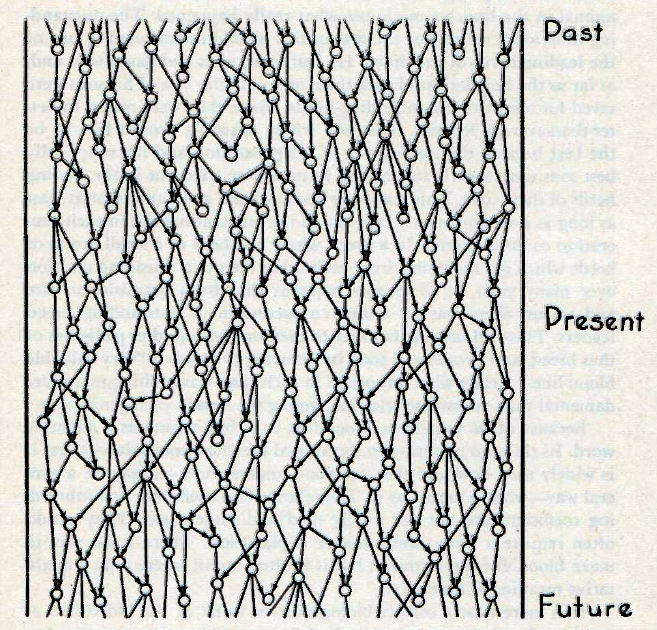
\includegraphics[width=\textwidth]{Figure_44.png}
    \caption{The pedigree of a population, showing that it is a network of descent
			 and is not composed of ``blood lines'' which are separate.}
    \label{fig:Lush_Figure_44}
\end{figure}

\section*{SUMMARY}

``Blood-line'' is an elastic term used sometimes as synonymous with
family, sometimes as a substitute for relationship, and sometimes to
describe vaguely a breeding system.

Because of its vagueness, blood-line is in bad repute as a scientific
term. But, because it is so widely understood by breeders, blood-line
will sometimes be found useful in conveying a general qualitative idea
about breeding topics where the speaker does not wish to call attention
to the quantitative aspect of that idea.
\index{Blood lines|)}

\newpage
\section*{REFERENCES}

\begin{hangparas}{0.5in}{1}%
\nowidow
Malin, D. F. 1923. The evolution of breeds. Des Moines: Wallace Publishing Company.
This book contains abundant references to blood and the word
``strain,'' or family. These show how one can speak more definitely on the
subject and yet avoid the use of ``blood-line.''

Whitney, Leon F. 1933. The basis of breeding. New Haven: E. C. Fowler. (Presents
many arguments against any use at all of ``blood'' to mean inheritance.)
\end{hangparas}
\chapter{Outbreeding Systems}
\label{cha:Lush_Chapter_26}
\index{Crossbreeding|(}
\index{Heterosis}
\index{Outbreeding|(}

Outbreeding is the general scientific term for mating animals distinctly
less closely related to each other than the average of the population
concerned. Its general effects are the opposite of those of inbreeding.
Outbreeding increases the heterozygosity of the individual and
increases the uniformity of the breed when it is first practiced, although
in a generation or two it comes to a limit in these respects. Continued
outbreeding merely serves to hold this individual heterozygosity and
breed uniformity. Any families which may have started to separate from
the rest of the breed are blended again toward the breed average by
crossing them with each other.

The practical usefulness of outbreeding rests on the general fact
that favorable effects of genes are apt to be dominant over the unfavorable
ones. Therefore, outbreeding increases the average individual
merit of the animals but lowers the breeding values of the best among
them. It increases at first the uniformity of the breed, but hampers further
progress in breed improvement. This superiority of the outbred
animals over the average of their parents in individual merit is so general
a phenomenon in many kinds of plants and animals that it has
been called ``hybrid vigor'' or ``heterosis.'' It is not often extreme unless
the parents are from different inbred lines or have in some other way
been made distinctly different from each other in the genes they carry.
The maximum practical usefulness of outbreeding systems is in the
production of market animals or purebred animals which are to be
shown to advertise the herd but which are not intended for breeding
use.

\section*{CROSSBREEDING}

Crossbreeding is the mating of two animals which are both purebred
but belong to different breeds. The mating of a purebred sire of
one breed to high grade females of another is often included under the
term crossbreeding.

Crossbreeding is often practiced in producing swine, sometimes in
producing poultry, and in some regions is extensively practiced by
sheepmen. Thus, in the northwestern range states many sheepmen plan
to keep one-quarter to one-half Merino or Rambouillet blood in the
ewes but use mutton rams on these ewes to produce market lambs.
Crossbreeding is rarer with cattle and horses; but there are certain
well-established practices of it, such as the production of blue-gray cattle for
feeding by crossing Angus and white Shorthorns, or the practice of certain
ranches --- e.g., the {SMS} ranch near Stamford, Texas --- in maintaining
an undercurrent of Shorthorn blood but of using bulls in the ratio
of 90 Herefords to 10 Shorthorns. Crossbreeding among cattle is also
practiced on a commercial basis along the Gulf coast, where many cattlemen
try to keep a quarter to a half Brahman blood in the cow herd,
but for siring the market steers and heifers use bulls from the beef
breeds which originated in Europe.

There have been many crossbreeding experiments with sheep, but
most of those have been planned to find what kind of ram is most profitable
for use upon range-bred ewes carrying a considerable amount of
Merino or Rambouillet blood. There have been several crossbreeding
experiments with swine to find how much general advantage there
might be in such crossing. The few crossbreeding experiments which
have been conducted with cattle have been directed mainly toward a
genetic analysis of the difference between breeds rather than toward
finding whether crossbreeding is a commercially successful practice.

Crossbreeding, like any other form of outbreeding, tends to lower
the breeding value of the individual by making it more heterozygous
and by making selection among the crossbred individuals less effective.
Like other forms of outbreeding it promotes individual merit because
of general dominance of genes favorable to size, vigor, fertility, etc.

When the crossbreds are used for breeding purposes, their offspring
are more variable than the crossbreds were and generally average
somewhat lower in individual merit. If both parents are crossbreds, the
offspring usually average below their purebred grandparents in individual
merit. Often the distribution of the offspring of crossbreds is
distinctly skewed, there being few which exceed the average of the crossbreds
and many which fall below it -- some of them far below.\footnote{Besides
the general dominance of favorable effects, it is probable that much of
this asymmetry in the distribution of the offspring of crossbreds is caused by gene
interactions such as those studied by Rasmusson (1933, \textit{Hereditas}, 18:245--61). In
more general terms it can be pictured as shown in Figures~\ref{fig:Lush_Figure_20}
\ref{fig:Lush_Figure_21}. The pure breeds crossed will usually have been in different
peaks, each more desirable than the adjacent genotypes. A general tendency to dominance
of the favorable effects of genes may keep the crossbreds high in individual merit. But
when the crossbreds reproduce, many of their offspring will fail to get some of the
genes vital for the successful functioning of the complete sets of genes which came
to the crossbreds from each of their purebred parents. Many of the offspring of the
crossbreds will, therefore, fall into some of the intervening valleys of low merit.}
But if one is to make full use of the heterosis of the crossbred females, it may
be necessary to use them for breeding. For example, in swine the number
of pigs farrowed and weaned and their weight at birth and probably
also at weaning are perhaps more dependent on the dam's characteristics
as a mother and nurse than on the genes which the pigs themselves
have, although the latter certainly play a part. It will be necessary to use
the crossbred females for breeding if this part of their heterosis is to be
used. Similar consideration would apply to egg production in poultry
and milk production in dairy cows. Some swine producers attempt to
solve this by keeping the crossbred gilts for breeding purposes and
breeding them to a purebred boar of a third breed. If all three breeds
nick well with each other in crosses, the pigs from such a ``triple cross''\index{Triple crossing}
should show many of the advantages of the original crossbreds besides
permitting their dams to show the effects of heterosis on their fecundity
and nursing ability. The triple-cross pigs are usually more variable,
since their crossbred dams transmit various combinations of genes to
them. The breeds can be chosen so that the triple-cross pigs will be as
uniform in color as the first-cross pigs. This is done by choosing for the
third cross a boar of a breed which has a conspicuous and dominant
color, such as solid white. This practice might theoretically be continued
to a fourth or even a fifth cross with only a little loss of heterosis in
the dams, but it becomes increasingly difficult to find more breeds which
are distinct from those already used and yet which nick well with all of
them. Actually this practice is rarely carried past the triple-cross.

\index{Crisscrossing|(}
``Criss-crossing'' is another method proposed\footnote{1935, Minnesota Agr.
Exp. Sta., Bul. 320.} for utilizing heterosis in the dams but not incurring
the full decline in average individual merit which usually occurs when
crossbreds are mated together. The plan is to use purebred sires all the time
but to alternate breeds. Thus, sows produced by crossing breeds \textit{A}
and \textit{B} would be mated back to \textit{A}. Their daughters (carrying
75 per cent of \textit{A} blood) would be mated to a \textit{B} boar. The
gilts thus produced (carrying 37\nicefrac{1}{2} per cent of \textit{A} blood)
would then be mated to an \textit{A} boar. If this were practiced regularly,
it would approach the condition in which each crop of pigs had \nicefrac{1}{3}
of its inheritance from one breed and \nicefrac{2}{3} from the other, but all
the sires used would be purebreds. The Minnesota Station reports good results
from this system, as far as it was carried in six years of experimenting. Some
practical difficulties with overlapping of generations are to be expected in
herds where only one boar is kept and is used both on gilts and on older sows.
This would not occur where all the sows are the same age. Figure 45 shows
examples of how pedigrees would appear after several generations of regular
criss-crossing or three-breed crossing.

\begin{figure}
	\centering
    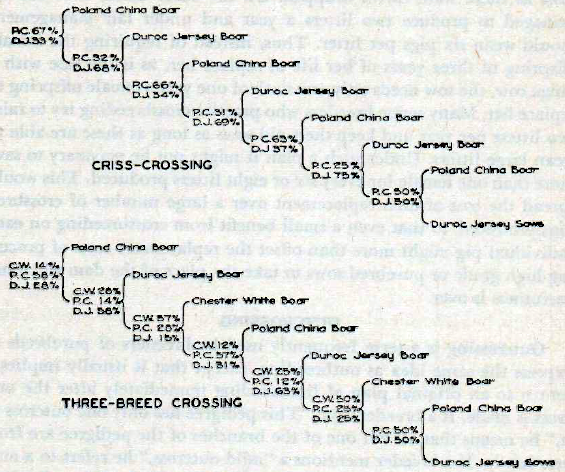
\includegraphics[width=\textwidth]{Figure_45.png}
    \caption{Illustrative pedigrees of ``criss-crossed'' and ``three-breed crossed'' pigs.}
    \label{fig:Lush_Figure_45}
\end{figure}
\index{Crisscrossing|)}

Whether crossbreeding is a sound commercial policy depends on
the balance between the extra size, vigor, fertility, etc., which is usually
gained by crossbreeding and the extra cost of replacement which is
incurred when the crossbred parents are replaced. Heterosis does not
occur uniformly in all crosses. That is, not all breeds nor all animals
within the same breed ``nick'' equally well. The heterosis from crossing
breeds of farm animals is not apt to be larger than around 2 to 8 per
cent increase over the average of the parental breeds for such things as
size, growth rates, fertility, or other complex physiological traits. It is
generally largest for vitality as measured by percentage raised of those
born. There is nothing in animal breeding to correspond to the very
large amount of heterosis which the corn breeders often find when they
cross two inbred lines. Presumably the underlying principles are the
same, but nothing corresponding closely to the inbred lines of corn
exists in the breeds of farm animals.

Crossbreeding is most likely to be profitable where fertility is highest
and the percentage of replacements necessary to keep up the female
herd is lowest. For example, with cattle under most range conditions 70
calves weaned per 100 cows per year is considered a good calf crop. With
half the calves being females, a herd would need to be kept three years
in order to produce enough females to replace the original cows even if
all heifer calves which lived to weaning time were used without selection.
If the average cow only stays in the herd about six to eight years,
nearly half of all her daughters will be needed to maintain the number.
If crossbreeding were practiced and all calves were sold for beef, this
would necessitate an annual replacement of about one-fourth as many
cows as there were calves dropped. On the other hand, sows can be
managed to produce two litters a year and under fair management
should wean six pigs per litter. Thus, instead of requiring the female
offspring of three years of her life to replace her, as is the case with a
range cow, the sow needs only one-sixth of one year's female offspring to
replace her. Many swine breeders who practice crossbreeding try to raise
two litters per year and keep their old sows as long as these are able to
wean large litters. Under such a plan it might not be necessary to save
more than one female for every six or eight litters produced. This would
spread the cost of each replacement over a large number of crossbred
pigs produced, so that even a small benefit from crossbreeding on each
individual pig might more than offset the replacement costs of procuring
high grade or purebred sows to take the place of the dam when her
usefulness is over.
\index{Crossbreeding|)}

\section*{OUTCROSSING}
\index{Outcross|(}

Outcrossing is a term frequently used by breeders of purebreds to
express the same idea as outbreeding, except that it usually implies a
return to an original plan of linebreeding immediately after the outcross
is made. If a breeder says: ``This pedigree has only one outcross in
it,'' he means that all but one of the branches of the pedigree are from
one family. If a breeder mentions a ``mild outcross,'' he refers to a mating
with an animal which is not quite of the family he is breeding but
which is related to it. A man after having practiced linebreeding for a
time may say that he needs an outcross. In this case he means that he
needs to mate his stock to animals from some other line; but the usual
implication is that, after one generation of outbreeding, he will return
to using animals of his original family, attempting by selection to hold
the good traits introduced by the outcross, while by linebreeding to his
chosen family again he tries to recapture and hold all the good traits he
already had in that family. The corn breeders call this kind of a process
``convergent improvement'' when used on their more intensely inbred
material.

Outcrossing is a minor part but eventually a necessary part of most
linebreeding programs. Any linebreeding which is carried far is apt to
fix some undesired traits so that mild outcrossing may be necessary to
remedy them. If the outcross is a success, the breeder is sometimes so
carried away by enthusiasm for it that he gives up his plan of returning
to his original family and decides to mate the outcrossed animals together.
To do this is the same in principle, although less extreme in degree,
as attempting to fix desired crossbred traits by breeding crossbred
females to crossbred males.
\index{Outcross|)}

\section*{BACKCROSSING}
\index{Backcrossing}

Backcrossing is the mating of a crossbred animal back to one of the
pure parent races which were crossed to produce it. It is a term commonly
used in genetic studies but not widely used by breeders. In
genetic analyses, particularly where one of the parents possesses all or
most of the recessive traits, the backcross permits a surer analysis of the
genetic situation than an $F_2$ generation does. General experience with
backcrosses in practical animal breeding has not been quite as satisfactory
as experience with crossbreds. The backcrosses retain some of the
heterosis in many cases, but rarely as much as the first crosses or the
triple crosses.

\section*{TOPCROSSING}
\index{Topcrossing}

Topcross usually refers to the last sire in a pedigree. When a breeder
mentions a ``Scotch-topped'' Shorthorn, he means a purebred Shorthorn
whose dam belongs to a family not originating in Scotland but whose
sire and perhaps maternal grandsire were ``straight Scotch.'' When a
breeder says that ``this animal has four topcrosses of Scotch blood,'' he
means that it is by a Scotch sire, that its dam is by a Scotch sire, that its
maternal grandam is by a Scotch sire and that the dam of the maternal
grandam is by a Scotch sire. Presumably the pedigree farther back in the
maternal line is not Scotch.

Top crossing is the same in principle as grading, except that topcrossing
is usually applied to different families within a pure breed,
whereas grading is applied to the continued use of sires of one pure
breed starting with foundation females which were of another breed or
of no particular breed at all.

In plant breeding topcrossing is sometimes used to mean the production
of seed by putting pollen from an inbred sire on plants from a
good commercial variety.

\section*{GRADING}
\index{Grading|(}

When the pure breeds were new and relatively scarce in this country,
grading common or mongrel stock up to the purebred level by the
continued use of sires of a pure breed was the quickest way available for
improving commercial herds. Many of the experiment stations conducted
experiments or demonstrations in the results of such grading.
Generally the first cross showed a marked improvement over the original
stock. The further improvement made by each successive cross was
progressively less. Grading can rapidly bring the stock near the level
of the pure breed which is being used for the grading. Grading will
remain the most important form of breeding for the commercial market
as long as the merit of the pure breeds is distinctly above that of
the commercial herds, and unless heterosis itself is so important that
wider out breeding plans, such as criss-crossing, are more profitable than
continued grading to one pure breed. The fact that in so many grading
experiments the major improvement has come in the first cross seems to
indicate that some of the improvement in the first cross was from heterosis.
No doubt the original mongrels in such experiments had at least
a few desirable genes which should have been kept if there had been any
way to select them and keep them while letting the rest of the genes
from the mongrels be bred out by the continued grading.
\index{Grading|)}

\section*{SPECIES HYBRIDS}
\index{Species!crosses|(}

The mule is the only commercially important species hybrid in
North American animal husbandry. Male mules are always sterile as far
as is yet known. A few well-authenticated cases of fertile mare mules
have been reported,\footnote{For two examples, see \textit{Jour. of
Heredity} 19:412--16, 1928.} but these have been so rare that they have
had no commercial importance. These fertile mare mules might possibly be
the means of transferring some characteristics from the ass species to the
horse species or the reverse. Because mules are sterile the problems of
mule breeding are only those of choosing the most suitable kinds or
breeds of mares and of jacks for crossing. The reciprocal cross, called a
``hinny,'' has been made many times, but is generally regarded as inferior
to the mule as a work animal.

Crosses between zebu cattle and cattle breeds of European origin
are of considerable economic importance in the Gulf coast region of the
United States and in nearly all the tropical regions of the world. Some
would regard these as species crosses, but the majority opinion is that
zebus and the cattle of European origin are not distinct species.
Intermediate types exist in the regions between their native lands, as in
southeastern Europe, Asia Minor, southern Siberia, and the northeastern
regions of Africa.

Crosses between European cattle and the American bison have been
made. Some would regard this as a generic cross. The males are sterile,
but many of the females are fertile. By backcrossing these females to
cattle and to bison, attempts to form a new breed, the ``cattalo,'' have
been made on a fairly large scale, but commercial success was not
achieved.

Other species crosses which involve farm animals but have hardly
passed the stage of zoological curiosities or menagerie specimens
include: horse and zebra, European cattle and yak, American bison and
yak, American bison and European bison or wisent, yak and zebu,
mouflon and domesticated sheep, bactrian and dromedary camels,
chicken and guinea hen, pheasant and hen, and peacock and hen.
Hybrids between yaks and other cattle are economically important in
some parts of China. Crosses between sheep and goats may start to
develop, but the embryos die and are resorbed or aborted long before
the normal gestation period is completed. A similar fate happens to the
embryos from crosses of chickens and turkeys.

Species hybrids do not seem to offer as much opportunity for economic
improvement in animal breeding as they do in plant breeding.
\index{Species!crosses|)}

\section*{SUMMARY}

Outbreeding generally leads to individual excellence but low breeding
worth.

Outbreeding systems hamper progress in further improvement of a
breed because they destroy families by constantly crossing together any
which start to develop. They thus make the breed temporarily more
uniform than if outbreeding were not practiced.

Crossbreeding is a special form of outbreeding where the parents
belong to different breeds. It generally results in increased size, vitality
and fertility; but the amount of this increase is variable in different
crosses. The economy of crossbreeding depends upon whether the
increase in these things is more than enough to balance the possible
confusion and increase in cost of replacements under a crossbreeding
system.

Crossbreeding is more apt to be profitable where fertility is highest
and females can be kept for the longest period of time and where the
cost of their replacement is lowest. Mainly for these reasons crossbreeding
is practiced most widely with swine and poultry and next with
sheep.

Outcrossing usually applies only to matings within a pure breed. It
may mean the same thing as outbreeding but usually implies also an
intention to return to the original family or strain after making the one
outbreeding mating.

Backcrossing is mating a crossbred animal back to the same kind of
animal as one or the other of its parents.

Topcross refers to the sire, maternal grandsire, and sires of the other
females in the purely maternal line. Generally it is used only within
pure breeds.

Grading is the continued use generation after generation of males
of one pure breed on an original foundation of another breed or of no
particular breed. Grading is the most economical way of lifting the
commercial stock rapidly toward the level of the purebreds.

\section*{REFERENCES}

For recent reports on experiments with crossbreeding, see the following
bulletins from agricultural experiment stations: Arkansas 411,
California 598, Iowa 380, Minnesota 320, Mississippi 347, Nevada 153,
Pennsylvania 279, and Wyoming 210. See also articles in \textit{Journal of
Animal Science} 1:213--20, and \textit{Scientific Agriculture} 16:322--36 and
19:177--98. Also see mimeographed leaflet BDIM-Inf. 30, May 1946,
from the USDA.
\index{Outbreeding|)}

%\textsc{Breeding Plans Based on Somatic Likeness}
\chapter{Mating Like to Like}
\label{cha:Lush_Chapter_27}
\index{Assortive mating|(}
\index{Mating like to like|(}

Although many writings on animal breeding stress the importance
of mating like to like, it is usually selection which is being discussed.
The familiar recommendation to ``breed the best to the best'' usually
implies that the worst (and the mediocre as far as numbers will permit)
are to be discarded. That would be selection, whereas mating like to
like would require also the mating of the worst to the worst and the
mediocre to the mediocre --- at least among those selected to be parents.

Actually some selection is always practiced; that is, the different
types are not permitted to reproduce at equal rates. The nearest actual
approach to mating like to like without selection occurs in breeds
where there is a marked disagreement about the ideal type, some breeders
working toward one goal and some toward another. So far as
concerns those traits on which there is disagreement, these cases show
some approach to the mating of like to like in the breed as a whole,
although in each individual herd the practice is merely selection. There
is a little of this at all times in all breeds because some breeders emphasize
certain characteristics more and other characteristics less than other
breeders do. Also a breeder who uses more than one sire at a time might,
if he chooses, mate the best sire to the best females, the second best sire
to the second best group of females, etc., until finally the poorest sire
among those he uses will be left for mating to the poorest bunch of
females which he keeps. This would be mating like to like within the
selected group. By contrast he might try to balance the groups of
females so that the mates of each sire would be about equal to the mates
of every other sire in average merit. This he might well do if his primary
object was an accurate progeny test of the sires. Or he might mate
the best male to the poorest group of females he kept, the second best
male to the next to the poorest group of females, etc. That would be
mating unlikes within the group selected to be parents. That is the subject
of the next chapter. ``Best'' and ``worst'' might describe net merit
or, for one characteristic at a time, we could be more specific by using
such terms as: largest or smallest, coarsest or most refined, most active
or most sluggish, darkest or lightest, etc.

These illustrations will show how any given intensity of selection
may be accompanied by any intensity of mating like to like, ranging
from almost perfect positive through random mating to almost perfect
negative. To see clearly what additional would be accomplished by
superposing a system of mating like to like on a certain intensity of
selection, which would be practiced anyhow, it is simplest to consider
how mating like individuals together, regardless of pedigree, would
change a population not under selection.

The fundamental difference in principle between inbreeding and mating
like individuals together regardless of pedigree is that inbreeding is
the mating of individuals which are apt to have the same genes, while
assortive mating is the mating of individuals which tend to have
\textit{similar characteristics}, irrespective of their relationship.
Characteristics are only partly caused by the genes, and it often
happens that characteristics which appear to be the same are caused by
very different combinations of genes. To the extent that variations in
characteristics are caused by environment or by epistatic deviations
or by dominance deviations, the mating of like individuals may cause
only a slight tendency for mates to be alike in the genes they have.
That can be expressed quantitatively as follows for purely assortive
mating. If \textit{m} is the correlation between the net hereditary
values of mates, \textit{t} the correlation between the visible or
measurable characteristics of mates, and \textit{h} the correlation
between the characteristic and the net hereditary value of the same
individual, then under purely assortive mating $m = h^2t$ and
\textit{m} cannot exceed $h^2$, even if the breeder has succeeded in
getting the mates to be perfectly alike (except for sex) in all
characteristics he can see or measure. On the other hand, under
purely inbreeding systems $t = h^2m$ and \textit{t} cannot exceed
$h^2$. As a numerical example consider a moderately heritable
characteristic for which $h^2$ = .2. Under purely phenotypic
assortive mating \textit{m} could not exceed .2 even if \textit{t}
were made perfect. In actual practice it would be less. By
contrast in the first generation of full brother-sister inbreeding
\textit{m} would be .5 and \textit{t} would be only .1. The actual
consequences of phenotypic assortive mating depend largely on what
size of m really is achieved. Hence they are very slight for
characteristics moderate or low in heritability.

The example shown in Table~\ref{tbl:Lush_Table_19} deals with
variation in only one characteristic. The practical breeder must
nearly always consider many traits. He will be using only one or
at most a few sires but will have several females, no two of which
are alike, to mate to each sire. Many of the animals he might
choose to mate together are alike in some characteristics,
moderately unlike in others, and perhaps extreme opposites
in still others. If he considers many characteristics, it will
be impossible for him to achieve in all respects a high degree of
resemblance between mates. This is in addition to the general
situation, discussed in the preceding paragraph, that under
assortive mating, likeness in net hereditary values will be less
than outward likeness. In actual practice assortive mating can
rarely cause \textit{m} to have high values for any characteristic
other than net merit.

\section*{ONE PAIR OF GENES}

If only one pair of genes is involved and if there is no dominance or
other reason for mistaking hereditary values -- i.e., if \textit{h}
and \textit{t} of the next to the last paragraph each equal 1.0 -- the
results are the same as in self-fertilization. If dominance is complete
but there is no other complication, the change is in the same direction
and the final result is the same but progress is slower. If the attempt
to mate like to like is not quite perfectly successful -- i.e., if
\textit{t} is less than 1.0 or if anything other than dominance makes
\textit{h} less than 1.0 -- the population will come to equilibrium
while a few heterozygotes still remain.

\section*{TWO PAIRS OF GENES --- SIMPLEST CASE}
\index{Variation!increased by mating like to like|(}

If this mating of like to like is for a characteristic influenced by two
pairs of genes, lacking dominance and with equal effects, then we have
the situation shown in Table~\ref{tbl:Lush_Table_19} which starts with a
random breeding population in which the two pairs of genes are independent
and the two alleles of each pair are equally abundant, that is, in which
$q_A = q_B = .5$.

\begin{table}[htbp]
	\centering
	\caption{\textsc{Proportions of Each Phenotype Under a Perfectly Accurate System of Mating
Like to Like,} $q_A$ \textsc{and} $q_B$ \textsc{Remaining at .5}}
	\label{tbl:Lush_Table_19}
	\begin{tabular}{C{2cm}|C{2cm}|C{2cm}|C{2cm}|C{2cm}|C{2cm}}
		\hline
		\hline
		~			& ~			& ~			& aa{BB}	& ~			& ~		\\
		~			& ~			& aaBb		& {AA}bb	& Aa{BB}	& ~		\\
		Genotypes	& aabb		& Aabb		& AaBb		& {AAB}b	& AABB	\\
		\hline
		~			& No Plus	& 1 Plus	& 2 Plus	& 3 Plus	& 4 Plus	\\
		Phenotypes	& Genes		& Genes		& Genes		& Genes		& Genes		\\	
		\hline
		Generation:	& ~			& ~			& ~			& ~			& ~			\\
		Start		& 6.2\%		& 25.0\%	& 37.5\%	& 25.0\%	& 6.2\%		\\
		1			& 13.6\%	& 20.8\%	& 31.2\%	& 20.8\%	& 13.6\%	\\
		2			& 19.3\%	& 16.5\%	& 28.4\%	& 16.5\%	& 19.3\%	\\
		3			& 23.9\%	& 13.8\%	& 24.6\%	& 13.8\%	& 23.9\%	\\
		$\cdots$	& $\cdots$	& $\cdots$	& $\cdots$	& $\cdots$	& $\cdots$	\\
		$\cdots$	& $\cdots$	& $\cdots$	& $\cdots$	& $\cdots$	& $\cdots$	\\
		$\infty$	& 50.0\%	& 0.0\%		& 0.0\%		& 0.0\%		& 50.0\%	\\
		\hline
	\end{tabular}
\end{table}

The result is a decrease in the proportion of the intermediate
phenotypes and a corresponding increase in the two extreme phenotypes.
If the mating of like to like is perfect and is carried on forever, it
approaches as a limit the condition in which all of the genotypes have
disappeared except the two homozygous extreme ones. If the mates are
not exactly alike phenotypically, as, for example, if an occasional mistake
is made in classifying an individual, progress will be slower, and
the ultimate goal will be an equilibrium which falls short of complete
fixation of the two extreme phenotypes.

This system of breeding tends to fix the extreme types, provided
those are both outwardly and genetically extreme; but, in contrast to
inbreeding, it cannot fix intermediate types. The likeness between parent
and offspring and the likeness between full brothers increases very
rapidly, although that may not be clear from this example. The variability
of the population is greatly increased, since the population tends
to become concentrated at the two extremes.

\section*{MANY PAIRS OF GENES}
\index{Genes, number of|(}
\index{Heterozygosis|(}

Many more than two pairs of genes may affect the characteristic,
and the effects of the different pairs of genes will rarely be equal. The
more genes there are, the slower is the rate of increase in homozygosis.
The likeness of parent and offspring or of full brothers also increases at
a slower rate when n is large, although these likenesses are not nearly
as much affected by changes in gene number as is the rate of increase in
homozygosis.

\section*{GENERAL RESULTS OF MATING LIKE TO LIKE}
\index{Homozygosis|(}

Very little genuine fixation of type is ever accomplished by this system
of breeding because increase in homozygosis is dependent upon the
number of genes being very small and upon the breeder's not being
deceived by dominance, environmental effects, or epistasis.
Figure~\ref{fig:Lush_Figure_46} shows what happens to homozygosis as a
result of mating like to like. Here \textit{n} is the number of gene pairs
involved, while \textit{m} is the correlation between the net hereditary
values of mates. Both \textit{m} and \textit{n} set limits on the amount
of homozygosis which may finally be attained, and \textit{n} has a
tremendous influence on the rate at which it is attained. Only with very
high values of \textit{m} and very low values of \textit{n} can such a
breeding system alter homozygosis much. The values of \textit{m} cannot
often be high in actual practice, and \textit{n} will probably be large 
for all characteristics of much economic importance.\footnote{The fraction
of the heterozygosis of a random breeding population which will still
remain when assort1ve mating has done all can is $\dfrac{2n(1 - m)}{2n(1 - m)+m}$.
Since \textit{m} cannot exceed 1.0 (it must usually be much smaller) and
\textit{n} can be large, this fraction will rarely be much less than unity.
\textit{Genetics}, 6:153.}

\begin{figure}
	\centering
    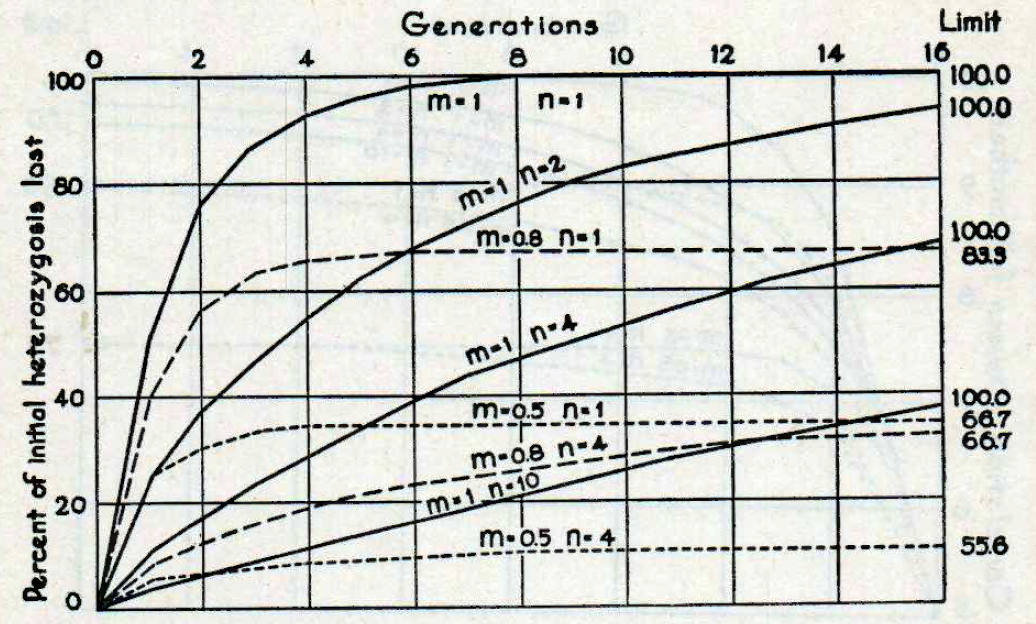
\includegraphics[width=\textwidth]{Figure_46.png}
    \caption{The percentage of initial heterozygosis which is lost by continued assortive
			 mating of various intensities, \textit{m}, and with \textit{n} pairs of equal
			 genes involved. (After Wright in \textit{Genetics}, 6:175.)}
    \label{fig:Lush_Figure_46}
\end{figure}

Mating like to like increases the resemblance of parent and offspring
very much, each individual resembling its sire not only because it
received half its inheritance from him but also because it received half
its inheritance from its dam who resembled the sire more than if mating
had been random. That is, the dam was chosen to have many genes
which produce the same kinds of effects as the sire's genes do, although
they may not be genes from the same allelic series. The limit which the
parent-offspring correlation approaches is determined by \textit{m}, large
\textit{n} merely making the approach to that limit a little slower. The
parent-offspring correlation goes far toward its limit in the first two
generations in which mating like to like is practiced.
\index{Homozygosis|)}

Figure~\ref{fig:Lush_Figure_47} shows what happens to the correlation
between full brothers under purely assortive mating in the extremely
simple case of no dominance, no epistasis, and no environmental
variations which are incorrectly discounted. The limits are determined
by \textit{m} and the only effect of large \textit{n} is to make progress
a little slower. This system of breeding has considerable effect, even
when \textit{m} is small and \textit{n} is large. The existence of
dominance and epistasis and environmental effects has the effect of making
\textit{m} lower than it need be otherwise. Environmental effects might
increase the correlations if these effects tended to be the same for brothers.
\index{Genes, number of|)}
\index{Heterozygosis|)}

A high degree of resemblance between parent and offspring and a
high degree of resemblance between full brothers seem to indicate that
the breeder is gaining control over his material, but that is partly contradicted
by the fact that there is little increase in real homozygosis.
This has long been recognized in a general way by breeders in the confidence
they have in the mating of like to like as a means of getting the
kind of herd they want, but again and again the more experienced
among them express the idea that inbreeding is really necessary if type
is to be ``fixed''

\begin{figure}
	\centering
    \includegraphics[width=\textwidth]{Figure_47.png}
    \caption{The correlations between brothers in successive generations
    		 under different degrees, \textit{m}, of assortive mating and
    		 with \textit{n} pairs of genes involved. (After Wright in
    		 \textit{Genetics}, 6:170.)}
    \label{fig:Lush_Figure_47}
\end{figure}

Mating like to like is one of the most powerful tools which breeders
have for creating extreme diversity in a population. Inbreeding tends
to fix intermediate families as well as extreme ones and thereby tends
to double the additive genetic variance of the population. But mating
like to like tends to scatter the population toward the two opposite
extremes of each characteristic for which it is practiced. For example,
assortive mating for stature within most local races of man is enough to
make the standard deviation about 20 or 25 per cent larger than it
would be if mating were entirely random with respect to stature. If the
characteristic is highly enough hereditary that \textit{m} in assortive
mating can rise above .5, mating like to like can make the standard
deviation in an unselected population larger than the most extreme
inbreeding can.\footnote{\textit{Genetics}, 6:154.} In each individual
herd the mating of like to like will usually be accompanied by selection
which will discard one or the other extreme. If all breeders select
toward the same ideal, this will not change the variability
of the whole breed any more than selection changes the variability
within a single herd. But if the breeders disagree markedly about the
ideal and some of them discard animals which other breeders think are
very desirable, this process can easily produce a lack of uniformity, in
the breed as a whole, so pronounced that everyone familiar with the
breed will be aware of it. Examples which have shown some tendency in
that direction are: ``Island type'' and ``American type'' in Jerseys;
``hot bloods'' and ``big types'' in Poland-Chinas. Even when all breeders
work toward the same ideals, a little of this herd heterogeneity within a
breed will arise because some breeders will try harder than others or
will be financially able to outbid others for the animals thought best.
Such inequality of striving toward the same ideal produces to a very
mild degree something of the same results as a divergence of ideals.
The changes brought about by purely assortive mating are temporary.
If there has been no accompanying selection, the population
returns far toward its initial condition in the very first generation after
random mating is resumed. In actual practice there will, of course, have
been some selection; and that is apt to have changed gene frequency
enough that the population will never return exactly to its initial
condition.
\index{Variation!increased by mating like to like|)}

\section*{SUMMARY}

Mating like to like has almost no effect on homozygosis except in
very simple and rare genetic circumstances.

Mating like to like immediately increases the resemblance between
parent and offspring and between full brothers.

Mating like to like comes near to the full limit of its effects within a
very few generations after it is begun.

Mating like to like tends to scatter a population toward the two
extremes with respect to each character for which such mating is practiced.
It, therefore, greatly increases the variability of the population if
both extremes are kept and heritability is high.

In actual practice mating like to like is always accompanied by
selection.

The effects of mating like to like disappear almost at once when random
mating is resumed, except as the accompanying selection may have
made some permanent changes in gene frequency.

\section*{REFERENCES}

\begin{hangparas}{0.5in}{1}%
Wright, Sewall. 1921. Systems of mating. {III}. Assortive mating, based on somatic
resemblance. Genetics, 6:144--61. (See also pp. 167--78.)
\end{hangparas}
\index{Mating like to like|)}
\chapter{Mating Unlike Individuals}
\label{cha:Lush_Chapter_28}
\index{Heterozygosis|(}
\index{Homozygosis|(}
\index{Mating unlikes|(}

The mating of unlike individuals (negative assortive mating on the
basis of somatic resemblance) is most commonly practiced either to
mark time while the breeder is deciding what his goal is to be or, where
the ideal is an intermediate, to correct defects by mating each animal
to one which is equally extreme but in the opposite direction. This is
sometimes called \textit{compensatory} mating.

Everyone does some of this from time to time, at least for minor
traits. There are no absolutely perfect animals. A breeder usually realizes
that his females are good in some respects but below his standard in
others. Under such circumstances he is almost certain to seek for his
next sire one which is particularly strong where his females are weak.
Since he cannot find a sire which is absolutely perfect in all respects, he
will accept one which is a little below his standard in characteristics for
which the females are unusually good. In the breeding of Rambouillet
or Merino sheep, it is common practice for breeders to seek ``light C''
rams to mate to their ``heavy B'' ewes and ``heavy B'' rams to use on
their ``light C'' ewes. Many are confident that this type of mating is
more apt to produce a high percentage of lambs which are on the borderline
of being the desired heavy C's or light B's than would be produced
from parents both of which were the desired type. Another
prominent example of mating unlikes is in the breeding of dual-purpose
cattle, where there is considerable mating of those which vary most
toward the extreme dairy type with others which vary most toward the
extreme beef type.

\section*{CONSEQUENCES}
\index{Genes, number of|(}

The consequences of mating unlikes are the reverse of those of mating
like to like. Heterozygosis is increased only a very little. The maximum
effect of mating unlikes, even if continued indefinitely, would be
to make the heterozygos1s $\dfrac{2n(1 - m)}{2n(1 - m) + m}$ of what it
would be under random mating, \textit{m} being negative. In the impossibly
extreme case when $m = -1.0$, that would increase the heterozygosis by only
$\dfrac{1}{4n - 1}$ of what it would be under random mating. That would
increase heterozygosis by one-third if only one pair of genes were involved,
by one-seventh if there were two pairs, only by one-eleventh if there were
three, etc. If the value of \textit{m} is nearer zero, the power of this
breeding system to affect heterozygosis will be still further reduced. When
\textit{m} is as near zero as $-.2$, the increase in heterozygosis cannot
exceed one-eleventh of the original amount even when \textit{n} is 1 and
cannot exceed one forty-seventh if \textit{n} is 4. Since \textit{m} must
usually be low and \textit{n} may well be large, it is obvious that average
homozygosis is scarcely affected at all.

The mating of unlikes\index{Variation!decreased by mating unlikes|(} together makes the correlation between parent
and offspring distinctly lower, since the two parents are quite different
from each other and the effects of the genes which an offspring
inherits from one tend to be canceled by the effects of the genes it inherits
from the other. Likewise, this system of mating tends to lower the
conelation between brothers, although not as much as the correlation
between parent and offspring is lowered.

Mating unlikes together tends to make the whole population uniform since an
extreme individual in one direction tends to be mated with one which is extreme
in the other. The offspring of each mating thereby usually average nearer the
population average than they would if mating were random. If mating were random,
there would be some matings where both parents happened to be extreme in the
same direction. This reduction in variability nearly reaches its limit within
the first and second generations after the mating of unlikes begins. In the very
first generation produced by mating unlike individuals, the variance becomes
$\frac{2 + m}{m}$ times what it was under random mating. Of course \textit{m}
is negative, but it has to be small unless heritability is high. The maximum
effect on the variability of a whole population occurs when \textit{n} is large
and \textit{m} is strongly negative. That maximum effect is to halve the variance
when $m = -1.0$ and \textit{n} is very large. If $m = -.4$, the maximum effect
is to reduce the variance two-sevenths when \textit{n} is very large and
one-sixth when \textit{n} is only 1. The original variability will reappear
almost at once when the mating of unlikes is abandoned.
\index{Genes, number of|)}

A system of mating unlikes is most useful when the desired type
is an intermediate. Under such conditions the maximum proportion of
desired individuals among the offspring can be obtained by mating
males which are of the desired type to females which are also of the
desired type and mating any breeding animals which deviate from the
ideal in one direction to those which deviate equally far in the other
direction.
\index{Heterozygosis|)}
\index{Homozygosis|)}

Mating unlikes together is extensively practiced commercially to
correct defects. This is a sound practice wherever there are enough
females undesirably extreme in one direction to justify the keeping of a
male equally extreme in the other direction.
\index{Variation!decreased by mating unlikes|)}

\section*{SUMMARY}

Mating unlikes together in the absence of selection leads to:
\begin{enumerate}
\item A more uniform population than under random mating, with a
larger percentage of intermediate offspring and fewer extremes in either
direction. This increased uniformity reaches nearly its full extent in
the first generation after the mating of unlikes is begun. If the mating of
unlikes ceases, the population returns almost at once to its original
variability under random mating.
\item Only a slight increase in heterozygosity under the very simplest
genetic situations and practically no change in heterozygosity under the
situations apt to be encountered.
\item A distinctly lower resemblance between parent and offspring and
a somewhat lower resemblance between other relatives than under random
mating.
\end{enumerate}
Mating unlikes is useful in holding the population together as a
more uniform group until the average type or some other intermediate
type can be fixed by close inbreeding.

Mating unlikes is useful in correcting defects wherever the ideal is
intermediate and some animals are too extreme in one direction while
others are too extreme in the other direction.

\section*{REFERENCES}

\begin{hangparas}{0.5in}{1}%
Wright, Sewall. 1921. Systems of mating. {III}. Assortive mating based on somatic
resemblance. Genetics, 6:144--6l. V. General considerations. Genetics, 6:167--78.
\end{hangparas}
\index{Assortive mating|)}
\index{Mating unlikes|)}

%\textsc{Other Topics Concerning Breeding Plans}
\chapter{The Relative Importance of Sire and Dam}
\label{cha:Lush_Chapter_29}
\index{Fertility|(}
\index{Sex linkage|(}
\index{Sire, importance compared with dam|(}

In general, sire and dam are equally important in inheritance.
There are three exceptions which are sometimes of practical importance.
The first is that a sire can have many more offspring in a single
season.\footnote{Monogamous species, such as pigeons, doves, and some
foxes, are exceptions to this. Among them the sire generally leaves about
the same number of offspring as the dam.} Therefore, the sire is much more
important than any one dam in determining the inheritance of the next
generation in the herd, although not more important in determining the
inheritance of any one animal. This is the basis for the common statement
that ``The sire is half the herd.''\footnote{This statement is an
exaggeration in the many cases where a sire is kept in service for less
than the average length of a generation. For example, in small dairy
herds, one sire is rarely used much more than two years; but the average
productive life of the cows is more nearly four years. Rarely are more
than half the cows in a herd daughters of one bull. Only half of their
genes come from him; hence one sire rarely furnishes more than a fourth
of the genes of the whole herd, although he does furnish half of the genes
of his own offspring.} The second exception is sex-linked inheritance. The
general rule in sex-linked inheritance is that sons are more like their
dams, and daughters are more like their sires than in ordinary inheritance.
The third exception is the one already discussed in
Chapter~\ref{cha:Lush_Chapter_14} that where the merits of the two parents
are not equally well known, less attention should be paid to the less well
known one in estimating the merits or breeding value of their offspring.

\section*{HIGHER FERTILITY OF THE SIRE}

When a breeder with a one-sire herd buys a sire, he is buying half
the inheritance of many offspring. When he buys a dam he is buying
half the inheritance of her sons and daughters only. Therefore, he can
afford to spend more money to procure a desirable sire than to procure
an equally desirable female.

Every individual has as many female as male ancestors. Becau se of
the larger number of offspring per male used for breeding than per
female, it is the usual rule that a breed is influenced more by some of
its males than by any equal number of females. However, about half of
what the male transmits came to him from his dam. It occasionally
happens that a female will exert more influence on a breed than any
contemporary male. A notable case is that of the Holstein-Friesian cow,
De Kol 2nd, whose relationship to the whole breed (about 10 per cent)
is more than that of any other cow or bull. She is almost a great
grandam of the whole breed today.\footnote{\textit{Jour. of Heredity},
27:61--72.} Naturally she could not exert this
much influence by having an enormous number of calves, although she
did live at least 16 years and produced 14 calves. She exerted her
remarkable influence on the breed through the fact that she had five
different sons which were quite prominent sires of the breed in their
time and saw extended service in leading herds. At least four other sons
and one daughter also left registered descendants. This is an exceptional
case, yet it illustrates how a female may exert a tremendous influence
on a breed if several of her sons are saved for extensive use. There is
some reason for thinking that more improvement in the dairy breeds
can be accomplished by the careful selection of cows which are to be the
dams of sires and therefore the grandams of the next generation than
can be done directly by selecting among the bulls. However, the exact
balance of the quantitative relations involved here is not yet clear.
\index{Fertility|)}

\section*{SEX-LINKED INHERITANCE}

In all farm animals except poultry, so far as is yet known, the male
has an \textit{X} and a \textit{Y} chromosome and the female has two
\textit{X} chromosomes. In poultry this situation is reversed. The
discussion which follows may be applied to poultry by substituting
the other sex.

Genes carried by the \textit{Y} chromosomes would, of course, be
transmitted from sire to son in unbroken lines if there were no
crossing over between \textit{X} and \textit{Y}. It would not be easy
to distinguish the effects of such genes from secondary sexual
characteristics. It is unlikely that the \textit{Y} chromosomes can
often, if ever, be entirely empty, or they would have been lost long
ago without harm to the species. Yet genetic research has found only
a few genes on \textit{Y} chromosomes.

In some species of fish, in man, and perhaps in most mammals, some
parts of the \textit{X} chromosomes are homologous with parts of the
\textit{Y} chromosomes and these can cross over. Genes carried in these
regions show ``partial sex-linkage.''\index{Partial sex-linkage} Their behavior is intermediate
between that of autosomal genes and that of the completely sex-linked
genes which are carried on the nonhomologous parts of the \textit{X}
chromosome. The latter are meant when sex-linkage is discussed in the
following pages. Examples of partially sex-linked genes in man are
those for retinitis pigmentosa and those for \textit{total} color
blindness. The genes for the ordinary red-green color blindness are
completely sex-linked.

The genes carried on the \textit{X} chromosomes are those responsible for
sex-linked traits. The male receives all of his sex-linked genes from his
dam; and, so far as those genes are concerned, he is no relative at all of
his sire. The female receives half of her sex-linked genes from her dam
and half from her sire just as with her other genes. But her sire can only
transmit one kind of \textit{X} chromosome to her, whereas the dam can transmit
either one of the pair she has. So far as daughters are concerned, this
amounts to the same thing as if the sires were completely homozygous
for their sex-linked genes, whereas the dams are as heterozygous for sexlinked
genes as they are for other genes. Consequently, paternal half
sisters will receive from their sire identical sex-linked genes; but
maternal half sisters need not be any more like each other in sex-linked
genes than they are in other genes. The following pedigree diagrams of
the \textit{X} and \textit{Y} chromosome situation for males and for females show what
happens when this is extended to the grandparental generation. The
notes show the part which each grandparent plays in the sex-linked
inheritance of the grandson or granddaughter.

\begin{figure}
	\centering
    \includegraphics[width=\textwidth]{Page_353.png}
\end{figure}

If it is assumed, on the basis of chromosome number, that about 5
per cent of the genes are sex-linked, then the expected statistical
effects of sex-linkage are those shown in the last two columns of
Table~\ref{tbl:Lush_Table_20}. The existence of sex-linkage will have
so small an effect that for most characteristics it would be difficult
to prove that there is any sex-linkage. Differences in the correlations
observed between various kinds of relatives have sometimes been
interpreted as indicating sex-linkage, but it is rarely possible to be
sure that such differences were not caused by (1) sampling errors, (2)
greater similarity of environment for some kinds of relatives or (3)
differences in the selection which had been practiced for various kinds
of relatives. It is to be expected that there will be some sex-linkage
in the inheritance of most characteristics which are affected by many
genes but that only rarely will a large fraction of the genes be
sex-linked. In such rare cases the corrections will more nearly approach
those in columns 1 and 2 of Table~\ref{tbl:Lush_Table_20}. The main point
which Table~\ref{tbl:Lush_Table_20} demonstrates is that only rarely will
sex-linkage alter resemblances noticeably.

\begin{table}[htbp]
	\begin{center}
	\caption{\textsc{Expected Effects of Sex-Linkage on Correlations$^*$ Between Males or Females and Various of Their Relatives}}
	\label{tbl:Lush_Table_20}
	\begin{tabular}{L{5.24cm}|C{1.25cm}|C{1.25cm}|C{1.25cm}|C{1.25cm}|C{1.25cm}}
		\hline
		\hline
		~			& \multicolumn{2}{C{2.5cm}|}{All Genes}	 & No Sex- & \multicolumn{2}{C{2.5cm}}{5\% of Genes} \\
		~			& \multicolumn{2}{C{2.5cm}|}{Sex-linked} & linkage & \multicolumn{2}{C{2.5cm}}{Sex-linked}	  \\
		\cline{2-6}
		~						& ~		& ~			& Male or	& ~		& ~		    \\
		~						& Male	& Female	& Female	& Male	& Female	\\
		\hline
		\textit{Ancestors}				& ~		& ~		& ~		& ~		& ~		\\
		\hspace{1em}Sire 							& .00 	& .71 	& .50 	& .487	& .512	\\
		\hspace{1em}Dam 	 						& .71	& .50	& .50 	& .512	& .500	\\
		\hspace{1em}Paternal grandsire				& .00	& .00	& .25 	& .244	& .244	\\
		\hspace{1em}Paternal grandam				& .00	& .50	& .25	& .244	& .268	\\
		\hspace{1em}Maternal grandsire				& .50	& .35	& .25	& .268	& .256	\\
		\hspace{1em}Maternal grandam				& .35	& .25	& .25	& .256	& .250	\\
		\textit{Collateral relatives}	& ~		& ~		& ~		& ~		& ~		\\
		\hspace{1em}Full brother					& .50	& .35	& .50	& .500	& .494	\\
		\hspace{1em}Full sister						& .35	& .75	& .50	& .494	& .515	\\
		\hspace{1em}Paternal half brother			& .00	& .00	& .25	& .244	& .244	\\
		\hspace{1em}Paternal half sister			& .00	& .50	& .25	& .244	& .268	\\
		\hspace{1em}Maternal half brother			& .50	& .35	& .25	& .268	& .256	\\
		\hspace{1em}Maternal half sister			& .35	& .25	& .25	& .256	& .250	\\
		\textit{Half first cousin (female)}	& ~		& ~		& ~		& ~		& ~	\\
		\hspace{1em}Through paternal grandsire		& .00	& .00	& .062	& .061	& .061	\\
		\hspace{1em}Through paternal grandam		& .00	& .25	& .062	& .061	& .083	\\
		\hspace{1em}Through maternal grandsire		& .18	& .125	& .062	& .073	& .067	\\
		\hspace{1em}Through maternal grandam		& .09	& .062	& .062	& .064	& .062	\\
		\hline
	\end{tabular}
	\end{center}
	$^*$For traits entirely determined by heredity, without dominance or epistasis and in a population breeding at random.
\end{table}

In breed lore there are many cases where a sire was noted for his
daughters but not for his sons, or vice versa. In Hereford history it is
said that the daughters of North Pole were exceptionally good individuals
but that his sons were not outstanding. All his sons were sold to
the range trade and passed out of the pure breed. The sons of Anxiety
4th in the same herd were regarded more highly, but among their offspring
those regarded most highly were out of daughters of North Pole.
It is possible that North Pole carried in his \textit{X}-chromosome desirable
genes which were largely missing from the other Hereford cattle of that
date. If that were the case, the use of his daughters' sons would be an
effective agency for spreading those genes through the breed. This is
probably the most conspicuous instance of the kind in animal breeding
history; yet it is more likely that the breeders, on observing the calves
of the two bulls, merely decided that the calves of Anxiety 4th were the
better. They could try out only a few bulls; so, of course, they kept the
sons of the better bull. Naturally they kept all of the best cows sired by
both bulls. At this date we will probably never know whether North
Pole really did carry sex-linked genes which were very valuable to the
Hereford breed but were not possessed by Anxiety 4th nor by many of
the other animals in the Gudgell and Simpson herd. This may have
been true, or it may have been largely an accident that the sons of
North Pole were all sold while many sons of Anxiety 4th were kept.

Alternative explanations of the same sort are usually available for
cases where it is reported that a certain sire produced remarkable sons
but ordinary daughters, or remarkable daughters but ordinary sons.
Sex-linkage is a possible explanation in such cases, but it is probable
that the major factor has usually been the selection which the breeder
practiced and whether he was at that time selling many males to head
other herds or was selling only females.
\index{Sex linkage|)}

\section*{SUMMARY}

Because the sire can have so many more offspring per year than the
dam, he is a more important individual than any one female so far as
the whole herd is concerned, although not more important so far as
concerns any one offspring.

This makes it possible to cull prospective sires more closely than
prospective dams and profitable to pay more for an unusually good sire
than for an equally good dam.

Every individual has the same number of female and male ancestors.
A female who has more than two sons which are widely used may exert
more influence on a breed than any one of her sons. This has actually
happened at times, although most animals which have influenced a
breed much have been males.

Sex-linked inheritance has the effect of making daughters resemble
their sires, and sons resemble their dams, more closely than if there were
no sex-linkage. This is not often important.

Most cases reported from animal breeding history where a certain
sire produced good daughters but ordinary sons, or the reverse, are
probably to be explained as incidental results of the sales or culling
policy in that herd. Sex-linkage may have played a part in some of these
cases.

\nowidow
Sometimes one side of the pedigree will seem to be more important
than the other merely because more is known about it, and therefore
more use can be made of it for prediction.

\section*{REFERENCES}

\begin{hangparas}{0.5in}{1}%
Gowen, John W. 1924. Milk secretion. Baltimore: Williams and Wilkins. (This book
includes correlations between the performance of various female relatives in
the Holstein-Friesian Advanced Registry.)

Madsen, Karl. 1932. Inheritance of milking capacity. Nature, January 30.

Pearl, Raymond. 1922. The biology of death. Philadelphia: J. B. Lippincott Company.
(See pp. 174 and 175 for correlations between various kinds of relatives
in man. Six different characteristics are included.)

Smith, A. D. B., and Robison, 0. J. 1933. The genetics of cattle. Bibliographia
Genetica X. (See pp. 46--51 for a review of the evidence on sex-linkage in the
inheritance of milk and fat production.)

Snyder, Laurence H. 1942. The mutant gene in man. Amer. Nat. 76:131--33.

Winge, O. 1934. The experimental alteration of sex chromosomes into autosomes
and vice versa, as illustrated by Lebistes. Comp. Rend. Laboratoire Carlsberg,
21:1--49. (An account of the sex-chromosome situation in this genus of
fish with much about sex-linked genes and about crossing over between the
\textit{X} and \textit{Y} chromosomes.)
\end{hangparas}
\index{Sire, importance compared with dam|)}
\chapter{Registering High Grades}
\label{cha:Lush_Chapter_30}
\index{Breed associations|(}
\index{Breed purity|(}
\index{Registration of grades|(}

For years after the registry associations were first organized, many of
them admitted to registry grade animals with a certain number of topcrosses
of registered sires. Nearly all of the American registry associations
have ceased doing this, and most of those which register a breed
native to other lands never did admit grades to registry in the United
States. Most of the European breeds still register females having three
or four top crosses of registered sires.\footnote{For example, the Shire
Horse Society in Britain admits mares with three topcrosses by registered
Shire stallions. Volume 4 of their ``Grading-Up Register'' in  1944
contained the pedigrees of 49 mares with one topcross and 41 with two
topcrosses, while 760 mares are entered in the contemporary Volume 64 of
the regular Stud Book.} In most cases those breeds also practice selective
registration (see chapter~\ref{cha:Lush_Chapter_16}). The proposal is
occasionally made that American breeds should also admit to registry high
grades which are outstanding individuals.

The pure breeds of today are comparatively modern developments.
Few have herdboks much more than 80 years old. Usually there was
no official herdbook until years after the breed had really been formed.
Naturally, at the time the herdbooks were established, the line between
registered and other animals was somewhat arbitrary. Often there was
disagreement as to whether certain animals really should have been
included in the herdbook. With this background for the history of
registration, the question automatically arises: What is wrong now
with registering grades, when that was done in the founding of all
breeds and still continues among many of them?

\section*{BREED HOMOZYGOSITY}
\index{Homozygosis|(}

The generations of strictly pure breeding that have elapsed since
registration began have enabled the breeders to make the breed somewhat
more homozygous than it was when the herdbooks were first
closed. The amount of \index{Heterozygosis}heterozygosity which was in the original
foundation stock but which has been lost solely through the pure breeding
since pedigree registration began can be measured by studying sample
pedigrees of the breed at any desired date. Those figures for the breeds
so far studied are as follows:

\begin{table}[h]
	\centering
	\begin{tabular}{L{8cm}R{3cm}}
	Shorthorn cattle in Great Britain 				& 26.0\% by 1920 \\
	Jersey cattle in Great Britain 					& 3.9\% by 1925 \\
	Ayrshire cattle in Great Britain 				& 5.3\% by 1927 \\
	Holstein-Friesian cattle in the United States	& 4.0\% by 1931 \\
	Hereford cattle in the United States 			& 8.1\% by 1930 \\
	Brown Swiss cattle in the United States 		& 3.8\% by 1929 \\
	Aberdeen-Angus cattle in the United States 		& 11.3\% by 1939 \\
	Clydesdale horses in Great Britain 				& 6.2\% by 1925 \\
	Rambouillet sheep in the United States 			& 5.5\% by 1926 \\
	Hampshire sheep in the United States 			& 2.9\% by 1935 \\
	Poland-China hogs in the United States			& 9.8\% by 1929 \\
	Brown Swiss cattle in Switzerland				& 1.0\% by 1927 \\
	Landrace swine in Denmark						& 6.9\% by 1930 \\
	Thoroughbred horse in the United States 		& 8.4\% by 1941 \\
	Standardbred horse in the United States			& 4.4\% by 1940 \\
	American Saddle horse							& 3.2\% by 1935 \\
	Telemark cattle in Norway						& 2.3\% in 23 years
	\end{tabular}
\end{table}

\noindent
These figures are probably no more than .5 per cent above or below
what would have been found if it had been possible to study the pedigrees
of all the animals of the breed. Evidently pure breeding by itself
causes only a slow drift toward homozygosity. The high figure for the
Shorthorns was mostly incurred in the first 30 years, most of it while
the breed was largely confined to the herds of the Colling brothers. For
the other breeds it appears that about one-half of 1 per cent ot the
remaining heterozygosity is being lost per animal generation.

The figures given do not include any changes in heterozygosity
which may have been caused by selecting animals which were more or
less homozygous than their pedigrees indicate. Selection changes homozygosi
ty only incidentally as a result of the changes it makes in gene
frequency. Selection requires a long time to change q enough to make
much change in $2q(1 - q)$ except where the genetic situation is simple
and selection is directed toward an extreme and the favored gene
already has a frequency above .5. Selection may have increased materially
the homozygosity of some genes which affect color, distinct
anatomical peculiarities, and other details of breed type for which the
genetic situation may be rather simple. But it is unlikely that selection
has changed very much the average homozygosity of the breeds for
genes affecting complicated characteristics. Selection for the effects of
heterosis may even have operated in the other direction to hold the
heterozygosity at a little higher figure than the pedigree studies indicate.
It seems unlikely that selection can have had much net effect on
the general homozygosity of the breed.
\index{Homozygosis|)}

\nowidow
These considerations make it reasonably certain that the purebreds
are more homozygous than the commercial stock, but doubtful that
their difference in this respect is extreme, even allowing liberally for
the fact that only a restricted group entered the registry in the first
place. Grades having at least four topcrosses\index{Topcrossing} of registered blood would
already be homozygous for about seven-eighths of the genes which were
homozygous in that breed but rare in other animals. The admission of
a few such grades would lower the breed's homozygosity very little.

\section*{INTRODUCING DESIRABLE GENES}

Some grade individuals are much superior to the average of the
purebreds in type or production or both. The best of these grades may
possess desirable genes which are either unknown in the pure breed or
are rare. The admission of these animals to registry might improve the
pure breed through introducing or making more frequent such desirable
genes. If females were required to have at least four topcrosses of
registered sires in order to be registered, only about one-sixteenth of
their genes would be other than those of the breed itself. This fraction
would be further halved in their offspring. The frequency of genes
already existing in the breed would not be changed much through the
admission of such grades. If there are desirable genes which do not now
occur at all within the pure breed, their introduction in this way might
be important.

\section*{GRADES SHOULD MEET HIGH STANDARDS AS INDIVIDUALS}

If the admission of grades is to improve the merit of the breed, the
advantage from introducing desirable genes should be greater than the
damage which would be done by upsetting the extra homozygosity
which the breed has already obtained. Such safeguarding could be
obtained by requiring the grade animal to meet distinctly higher standards
of individuality and production than the average individual merit
of the animals already registered. Just how much higher than the
breed average these standards of individual merit should be for grades
for which registry is being asked would depend in principle upon how
different the pure breed really was from the foundation stock from
which this grade was produced. Any standards adopted would necessarily
be somewhat arbitrary.\footnote{For an example of standards of this kind in
actual operation in Sweden, see \textit{Hoard's Dairyman}, 74:62.}

\section*{DISRUPTING EPISTATIC COMBINATIONS}
\index{Epistatic effects|(}

It is possible that the present merit of the various pure breeds
depends in part upon certain combinations of genes which produce
good results as a combination but not separately. One such combination
might be typical of one breed (although of course not entirely homozygous
in all animals of that breed), while very different combinations
which have the same general kind of effect may be typical of other
breeds. If so, the admission of even a little outside blood to the breed
might scatter those epistatic combinations enough to lower merit more
than the small percentage of outside blood admitted would indicate.

While this is theoretically a possibility, yet there seems no way to
estimate whether such situations are frequent enough to be important.
Even if such situations are frequent, grades carrying as many as four
topcrosses of the pure breed would already have most of the genes
which are necessary for such combinations. That makes the theoretical
danger of harming the breed in this way seem rather remote. The existence
of even a slight possibility of such damage is an additional reason
for requiring that any grades to be admitted should meet standards of
individual merit distinctly higher than the average of the pure breed
into which they come.
\index{Epistatic effects|)}

\section*{ADMISSION OF PUREBREDS WHICH ARE NOT NOW ELIGIBLE TO REGISTRY}

It often happens that a purebred animal cannot be registered
because the breeder is not certain of its sire. The breeder may be certain
that the sire of the animal was one of two or three males, all of
which were purebred, but he may not have any record of the breeding
date, or the actual birth date may be far from the expected one. Economical
use of range resources often requires several males for each
group of females. If the females are all purebred and the males are all
purebred, all the offspring are purebred, too; but their individual
pedigrees are not known and they are not at present eligible to registry
in any association. Sometimes outstanding individuals are produced
from such flocks or herds, and the breeder would like to use them for
stud purposes if they could be registered. Several sheep associations in
the United States have discussed proposals for such \index{Flock registration}
``flock registration,''
but none have been adopted. Such ``flock registration'' would not lower
the homozygosity so far attained in the breed. A breeder using such animals
could still use mass selection in improving his livestock but could
not make much use of ancestors and collateral relatives to estimate
breeding worth. Such a proposal might have unexpected consequences
on the finances of the registry association, but that might be controlled
by adjusting the fees for flock registration. Flock registration is a well
established practice with sheep in many other lands, notably Australia.

\section*{ECONOMIC AND PSYCHOLOGICAL CONSEQUENCES}

To admit high grades to registration might lower the breed reputation
with those who set the highest value on absolute purity of breeding.
This might be offset, at least in part, by the fact that some would
construe such action to mean that individual merit was so highly
respected in this breed that something in pedigree desirability would
be sacrificed to attain unusual individual merit.

The registration of high grades would increase the supply of registered
animals and, therefore, might tend to lower the prices which
could otherwise be obtained by those who already have the purebred
individuals. This could be controlled by having the requirements of
individuality and productive ability so high that only a few grades
would be admitted. Apparently this actually happens abroad. In most
breeds where grades having at least four topcrosses of registered ancestry
may be admitted to registry, only a small number are thus admitted
each year. This slight increase in supply might be more than offset by an
increased demand from those commercial producers who might be
favorably impressed by the evident interest of that breed in individual
merit. Just how those two factors would balance is not clear, but it
seems unlikely that enough high grades would ever be admitted to registry
to be an important economic factor.

Breeders would disagree about the wisdom of admitting any high
grades at all to registration. If any breed does undertake such registration,
it is likely that the official pedigrees will indicate which animals
are absolutely purebred in all lines and which trace to some of those
admitted high grades. Thus, the advocates of absolute purity could
avoid pedigrees tracing in any line to the grades. Something of that kind
actually happens unofficially in the case of pedigrees where there is suspicion
but not absolute proof of fraud. Those who know the situation
let such animals strictly alone, treating them as grades. There is thus a
tendency to eliminate them from the breed, although a beginner unfamiliar
with the situation will sometimes pay purebred prices for them.
After many generation.s an official system of indicating those which
trace at all to grades might break down with its own complexity; but
long before that time had arrived, the breeders would either have
revoked the registration of grades or would have come to substantial
agreement that it was a sound policy.
\index{Breed purity|)}

\section*{SUMMARY}

The registration of high grades unusually superior in individual
merit is a common practice with many European breed associations but
is practiced by very few associations in the United States.

The genetic consequences of such a practice are: (a) Some loss in
homozygosity, and (b) the possibility of introducing some desirable
genes which are rare or unknown in the pure breed.

If the grades were required to meet distinctly higher standards of
individual merit and productivity than the average of the purebreds,
the gain to the breed through the increase of desirable genes would be
likely to be greater than the harm through loss of homozygosity.

Some animals which are absolutely purebred cannot now be registered
because of uncertainty about which of two or more purebred animals
was the sire. The admission of such animals to registry through a
plan of ``herd registration'' or ``flock registration'' would not result in
any loss of the breed's homozygosity. It might lead to a little breed
improvement if only superior individuals were registered, although the
selection of such superior individuals could be little more accurate than
simple mass selection in general.

Economic reasons will predominate in decisions about the registration
of grades. There might be some loss through the breed's appearing
less strict in its standards of purity than its competitors. There might
be some gain through advertising that individual merit was receiving
special attention in that breed.
\index{Breed associations|)}
\index{Registration of grades|)}

\section*{REFERENCES}

For accounts of the increase in homozygosis in various breeds, see
the references at the end of chapter~\ref{cha:Lush_Chapter_21}. For
other articles dealing more directly with the possibilities of
registering high grades or with differences between grades and
purebreeds, see the following:

\begin{hangparas}{0.5in}{1}%
Anonymous. 1927. A challenge to pure breeds. \textit{Hoard's Dairyman},
72:126--27. Feb. 10.

Anonymous. 1929. Admit grades to registry. \textit{Hoard's Dairyman},
74:637. July 10.

McDowell, J.C. 1928. Comparison of purebred and grade dairy cows. USDA,
Cir. 26.

Peterson, Guy A. 1929. Swedish herdbook registration. \textit{Hoard's
Dairyman}, 74:62.

Savage. E. S. 1936. Registration of grade cattle. \textit{Hoard's Dairyman},
8l(9):242. May 10.
\end{hangparas}
\chapter{Sire Indexes}
\label{cha:Lush_Chapter_31}
\index{Progeny test|(}
\index{Sire indexes|(}

A sire index is a way of expressing what the sire's progeny indicate
about his heredity. It is most needed for characteristics which the sire
cannot show himself: milk and fat production in dairy cattle, egg production
in poultry, prolificacy in swine and sheep, nursing ability in all
mammals, and certain traits of disposition which are expressed differently
in males and females,\footnote{Hammond, John, 1932, \textit{Report on
Cattle-breeding in Jamaica and Trinidad}, Publication No. 58 of the Empire
Marketing Board, London.} etc. For characteristics which the sire can
manifest in himself, a sire index is useful for revising estimates of his
hereditary value when such estimates have been based only on his own
characteristics and on his pedigree.

A complete sire index would logically be based on all available
information about the sire's own characteristics and about his ancestors
and collateral relatives, as well as on the information about his progeny;
but most of the current discussion about sire indexes deals only with
ways to use the information about the progeny and their other parents.
Sire indexes of that kind are only special applications of the principle
of the progeny test discussed in chapter 15. Sire indexes are mentioned
most often in writings on dairy and poultry breeding.\footnote{See
\textit{Jour. of Dy. Sci.}, 16:501--22, for a discussion of the general
principles involved.} The wording used in the rest of this chapter applies
primarily to dairy cattle. The principles are the same in other cases, but
the importance of some of the considerations may change.

\section*{THEORETICAL BASIS}
\index{Sampling nature of inheritance|(}

The reasons for computing a sire's index as $2D - M$, when \textit{D} is
the average of his daughters and \textit{M} is the average of the dams of
those daughters, may be seen from the equations on page \pageref{eqn-page-198}.
The reasons for not trusting the index completely arise from what are called
``Mendelian errors'' and ``errors of appraisal'' in those equations.

The Mendelian errors come from chance at segregation which permits
gametes coming from the same parent to contain different genes,
so that some offspring are genetically better than the average of their
parents while others are worse. These variations are truly random, provided
the daughters are an unselected sample. Therefore, they tend to
cancel each other and their importance in an average diminishes as the
number of daughters increases.

The errors of appraisal come from the fact that even after we have
corrected the record of a daughter or a dam for age, for times milked
per day, and for every other non-standard environmental circumstance
about which we know, the record will be higher in some cases and lower
in others than corresponds to the real breeding value of the cow. Such
of these errors as are random tend to diminish in importance as the
number of daughters in the average increases, just as the Mendelian
errors do. Some of the errors of appraisal are not random but tend to be
in the same direction for all the daughters or for all the mates of the
same bull but may be in a different direction or be different in size for
the daughters or mates of other bulls. They may even be different for
the daughters and for the mates of the same bull. Frequent causes of
these biased errors are: (1) The general level of environment to which
each group of daughters or of dams was exposed may have varied much
from one group to another and we may not know what the environment
was in each case, or may know it but not be able to allow perfectly for
its effects. (2) The daughters or the records which were used to represent
them may have been selected ones, rather than a fair sample of all.
(3) The dams of these daughters may have been a selected group and
the intensity of that selection, too, may have varied from one sire to
another. Such biased errors do not tend to cancel each other as the
number of daughters increases.

The actual numerical value of each sire index is partly determined
by the real breeding value of the sire but partly also by whatever biased
errors that index contains and by the uncanceled remainder of the random
errors. Accordingly sire indexes will vary more than the real breeding
values of the sires do. The sires with the very highest indexes are
generally good sires but they are not likely to be as good as their
indexes. Similarly the sires with low indexes are generally poor sires
but they are not usually as poor as their indexes. We shall make the
smallest mistakes if we estimate the breeding value of each sire at part
way between his index and the average of his breed.
\index{Sampling nature of inheritance|)}

The principles governing how much confidence the index deserves
can best be understood by considering first the dependability of an
index (\textit{I}) based on the record of only one daughter (\textit{D})
and her dam (\textit{M}). The variance of \textit{D} and of \textit{M}
will be nearly the same. For clarity in the argument this variance can
be divided into the additively genetic portion (\textit{G}) plus a portion
(\textit{E}) due to random discrepancies between the genetic value and and
the record of the cow, plus a portion (\textit{C}) due to those
discrepancies between record and breeding value which are alike for all
the daughters of a bull or for all the mates of a
\newpage
\noindent
bull. Then, according to the usual formula for the variance of a difference,
the variance of the index is:

\[ 5G + 5C + 5E - 2G - 4xC = 3G + (5 - 4x)C + 5E \]

\noindent
where \textit{x} is the correlation between \textit{C} for a daughter and
\textit{C} for her dam. The sire's breeding value is responsible for only
\textit{G} of the variance in this index, as may be seen by referring to
diagram \textit{B} in Figure 32. That diagram shows how the genetic value
of an individual is \nicefrac{1}{4} determined by the genetic value of its
sire, \nicefrac{1}{4} by the genetic value of its dam and \nicefrac{1}{2}
by chance at Mendelian segregation.\footnote{If sire or dam were inbred,
the fraction determined by the genetic value of that parent would be
$\dfrac{1+F}{4}$, while correspondingly less part would be determined by
chance at segregation. In most populations inbreeding is unusual and is so
mild that we can ignore it here with little error.} The genetic variance
which the dam determines is removed in subtracting \textit{M} from
\textit{2D}. That leaves in the variance of \textit{I} only \textit{3G}
of the \textit{4G} which is the genetic variance in \textit{2D}. The sire
is responsible for \nicefrac{1}{3} of that \textit{3G}, while chance at
segregation is responsible for \textit{2G}.

When the index is based on n daughter-dam pairs, instead of one,
the random parts of the variance in \textit{I} become only
\nicefrac{1}{\textit{n}} as large. Thus the variance of \textit{I}
based on \textit{n} pairs is: $G + (5 - 4x)C + (2G + 5E)/n$.
The equation which will predict with the least error the breeding value
of the sire becomes:

\[ Sire - A = \dfrac{n}{n[1 + (5 -4x)C/G] + 2 + 5E/G}(I - A) \]

\noindent
where \textit{A} is the breed average. The fraction in this equation can be
considered as showing the extent to which the index should be believed.
The square root of this fraction is the correlation between the index
and the real breeding value of a bull.

\index{Heritability|(}
Wright has discussed this equation for the case of complete heritability;
i.e., when \textit{C} and \textit{E} are both zero. Then it becomes simply:
\(Sire - A = \dfrac{n}{n + 2}(I - A)\) and confidence in the index becomes almost
complete when the number of daughter-dam pairs is much more than
five. This, however, is not very realistic because in practice \textit{E} will
always be real and for many characteristics it will be much larger than
\textit{G}. \textit{C} also is likely to have a real value in most sets of data
which are collected from many herds, since it is rarely if ever possible to
discount accurately for all of the differences in management and environment
from one herd to another.

The effects of \textit{E} may be seen most clearly by considering the case in
which \textit{C} is zero but heritability \(\left(i.e., \dfrac{G}{G + E}\right)\) varies.
Then the fraction in the prediction equation becomes: \(\dfrac{n}{n + 2 + 5E/G}\)
which takes values such as the following:

{\renewcommand{\arraystretch}{2}%
\begin{table}[h]
	\centering
	\begin{tabular}{C{2cm}C{1cm}C{2cm}}
	Heritability	& & Fraction			\\
	.10				& & $\dfrac{n}{n + 47}$	\\
	.20				& & $\dfrac{n}{n + 22}$	\\
	.25				& & $\dfrac{n}{n + 17}$	\\
	.33				& & $\dfrac{n}{n + 12}$	\\
	.50				& & $\dfrac{n}{n + 7}$	\\
	.71				& & $\dfrac{n}{n + 4}$	\\
	1.00			& & $\dfrac{n}{n + 2}$
	\end{tabular}
\end{table}}

\noindent
If \textit{E} is large the justifiable confidence in the index is obviously
very low when \textit{n} is small. Nevertheless perfect trust in the index
is approached, although slowly, as \textit{n} becomes extremely large.
\index{Heritability|)}

\index{Regression|(}
The existence of \textit{C} changes the situation so that confidence in the
index increases more slowly with \textit{n} and no longer approaches unity
as a limit. Instead it approaches $1/y$ where $y = I + (5 - 4x)C/G$. This
\textit{y} can be a large number if \textit{C} is large relative to \textit{G}
and if \textit{x} is small. That
$C/G$ may often be as large as 1.0 in dairy data is indicated by correlation
usually of the order of .2 to .3 between the records of unrelated or
slightly related cows kept in the same herd. The general size of \textit{x}
is less certain. It would be 1.0 if all of \textit{C} came from general
differences in environment from herd to herd and if the peculiar environment
of each herd were unchanging, year after year. However, part of \textit{C}
can come from herd environment which changes between the time when the
dams made their records and the time when the daughters made theirs.
A part of \textit{C} can come from selection of the dams or of the daughters
having been more intense for some bulls than for others. Hence \textit{x}
will not be 1.0 although it may usually be above .5. The case $C = G$ and
$x = .5$, which is not unreasonable for dairy data, will illustrate the
power of \textit{C} to limit confidence in the index. In that case confidence
in the index will not exceed \nicefrac{1}{4}, even when the number of daughter-dam
pairs becomes exceedingly large. If \textit{C} is only half as large as
\textit{G}, the corresponding limit is \nicefrac{2}{5}. If \textit{C} is as large
as \textit{G} but \nicefrac{3}{4} of \textit{C} is alike for the daughters and
for the mates of the same bull, the limit is \nicefrac{1}{3}.
\index{Progeny test|)}
\index{Regression|)}

Obviously anything which can be done to diminish \textit{C} and
\textit{E} by keeping the environmental conditions standard and
alike for all daughters and dams, or by correcting the actual
records for the effects of varying environment or of unequal
selection of the mates of various bulls will increase the confidence
which the index deserves.

\section*{PRACTICAL CONSIDERATIONS}

\textsc{Relative rating}. For comparing bulls with one another when all
of them have the same number of daughter-dam pairs, the index is all
that is needed since it will then rank all the bulls in the same order and
proportionately the same distance apart, no matter what is the value of
\textit{C} or \textit{E} or \textit{x}. The need for knowing how much to
regress the indexes toward the breed average arises only when we wish to
compare bulls proven on different numbers of pairs, or when we wish to
compare a bull's index with a cow's record. For the first of these purposes
ignorance of \textit{C}, \textit{E}, and \textit{x} makes only a little
difference unless n varies extremely from one sire to another. Doubling
\textit{n} will double the numerator but only the first part of the
denominator. If that first part of the denominator is already more than
half of it, the doubling of \textit{n} will increase the fraction by less
than one third of its initial value. Hence further increases in \textit{n}
when it is already large add only slightly to the confidence which the index
deserves.

\textsc{Comparing bulls' indexes with cows' records}. The necessity for
comparing a bull's index with the records of a cow is met almost every
time we evaluate a pedigree in which the sire or one or both grandsires
are proven. For example, in choosing between young bulls \textit{A} and
\textit{B} we may find that the sire of \textit{A} has an index which
is 40 pounds higher than the index of \textit{B}'s sire but that the
records of \textit{B}'s dam average 60 pounds higher than the records of
\textit{A}'s dam. To estimate whether \textit{A} or \textit{B} probably
has the higher breeding value, we have to decide whether a difference of
40 pounds in sire indexes is as important as a difference of 60 pounds
in the records of cows. If the cow's record is left in its actual
form, sire indexes can be compared directly and fairly with it if the
indexes have been regressed only enough that they would have about
the same variability as the cows' records -- a little more variability if an
index is generally a bit more accurate as an indicator of a sire's breeding
value than a cow's record is of her breeding value, but a little less
variability if the indexes are generally less accurate. If the indexes are
each numerically equal to the estimated breeding values of the bull to
whom it belongs, then the cow's record also should be regressed far
enough toward the breed average to make it likewise an unbiased estimate
of her breeding value. Present practice in this respect is not uniform.
The Holstein-Friesian Association publishes indexes based on six
or more pairs and does not regress them at all. This makes these indexes
just a bit more variable than the records of cows with one record each.
The same is true of the indexes computed by the American Dairy Cattle
Club from the records published by the Dairy Bureau of the USDA,
except that in this case the minimum number of pairs is five. The Ayrshire
Association since late 1944 has been regressing sire indexes half
way toward the breed average and basing them on at least ten pairs.
Sire indexes regressed this much are only about half as variable as records
of cows who have one lactation each.

\textsc{Number of daughter-dam pairs needed.} From the principles governing
the accuracy of sire indexes it is clear that accuracy is low when
the number of pairs is very small but it is also clear that accuracy does
not suddenly become perfect when a certain number is reached. Instead
the accuracy increases at an ever-decreasing rate as the number rises.
Since the gain from increasing n comes solely from the decrease which
that makes in the term $(2G + 5E)/n$ in the variance of \textit{I}, the
advantages in having \textit{n} any larger have mostly been reaped by the
time $(2G + 5E)/n$ has already become distinctly smaller than $G + (5-4x)C$.
\noclub

Largely by trial and error but partly based on considerations like
these, all official plans for computing indexes specify some minimum
number for \textit{n} before an index will be computed at all. One important
consideration which has kept the minimum numbers small is that if
many daughters were required few bulls could be proved. Those who
made the Dairy Bureau policy thought that the increased accuracy
which the proof would have, if six were required instead of five, would
be more than offset by the fact that the large number of bulls who have
only five comparisons would thereby not be brought to the attention of
breeders who might otherwise hear of them and make some use of that
information. There is good reason for believing this still to be sound
policy, although the original decision was made years ago. One suggestion
for reaping both advantages is that bulls be given a preliminary
index when five pairs are available and another index when the number
has risen to another level, for example eight or ten. The Ayrshire
Association does something of this kind. This, however, adds to the
bookkeeping and some customers will not distinguish between the bulls
with only preliminary proof and the bulls with more complete proof.

\textsc{Simplicity} of the index is important for explaining
it to the potential users and giving them the proper amount of confidence
in it, for ease and speed of computing it, and to reduce the chance of
clerical errors. Yet the underlying principles are such that at least a
little accuracy must be sacrificed if simplicity is to be achieved in data
in which \textit{n} varies or if the same index is to be used in different
populations, such as Dairy Herd Improvement Associations or Herd Improvement
Registry, in which the relative proportions of \textit{G}, \textit{C} and
\textit{E} may vary. When breed associations or other agencies compute and
publish indexes as an impartial service to buyers, they have to compromise
a little on accuracy in order to achieve the uniformity and simplicity which
is necessary for getting the index used . Whether it is better merely to
publish $2D - M$ and let the user do all the discounting of this for
\textit{C}, \textit{E} and small \textit{n}; or to regress it automatically
half way toward the breed average as the Ayrshire Association is now doing,
or to regress it some other fraction (perhaps one fraction for test, a
different one for fat, another for type, etc.), is still open to argument.
The issues involved are largely psychological ones centering on what
procedure actually will get most breeders to use the indexes with most
nearly the proper degree of confidence and with the least confusion and
disappointment.

\index{Selection!and sire indexes|(}
\textsc{Selection of daughters} will bias the index to an extent for which
good correction can be made only in the unlikely event that one knows
how intense the selection was and on what it was based. If the number
tested but omitted from the average is known, it can be assumed that the
missing ones had lower records than any of those given. For example,
if we read that a bull had 10 daughters which averaged 600 pounds in a
Dairy Herd Improvement Association but we happen to know that ten
other daughters of his were tested, we can see by Table~\ref{tbl:Lush_Table_12}
that the high half of a normal distribution averages .8 of a standard
deviation above the average of the whole group. With the intra-herd
standard deviation in such data being around 80 pounds of fat, we can
estimate that the average of all 20 daughters was about 600 minus 64
or 536 pounds, but that could easily be 30 or more pounds in error
with numbers this small and with the distribution perhaps not being
exactly normal. As another example, suppose we are told that a certain
bull has 30 Advanced Registry daughters, five of which have records
over 800 pounds. It is safe to assume that these five are the very
highest. By consulting appropriate tables for the normal curve we
learn that the point above which the highest one-sixth of the
population lies is about one standard deviation above the average
of the whole group. Since the intra-herd standard deviation in Advanced
Registry data is about 100 pounds, we would estimate that the average
of all 30 daughters was about 700 pounds, but this could be considerably
in error, especially since the numbers are small and the distribution
of Advanced Registry data is not quite symmetrical.

If the missing daughters were not even tested, corrections for their
absence are even more in doubt since one cannot then assume that their
average would have been low. Some may have died while yet young,
some may have been culled intentionally on type or pedigree, some
may have been sold into herds in which no testing was done, some may
have been started on test and then removed (in the testing plans which
permit that) when it was seen that they would do poorly, etc.

Considerations such as these have led breed associations to compute
indexes only with data from those systems of testing in which it is
required that all animals in the herd be tested if any are. Also it is only
reasonable for such agencies to inquire about the missing daughters.
Some associations are not able to do more about this than to publish,
along with the average of the tested daughters, the total number of
daughters old enough to have had a record. This can give the reader
some notion of how much possibility there was for selection among the
daughters of each sire.

There is no way wholly to avoid natural selection among the daughters.
More of the constitutionally weak or sickly daughters than of the
normally healthy ones will be barren or will have died before they
could be tested. Also it is to the immediate economic interest of the
breeder to cull the extremely unpromising heifers as soon as he knows
they are such, without incurring the expense of keeping them through
their first lactation. However, the correlation of outward appearance
or pedigree promise with actual performance is low enough that the
effects of such culling prior to testing are much smaller than the effects
of omitting daughters after their records are already partly made. It
has been proposed but never officially adopted that in proving a sire
each daughter old enough to have a record, but without one and without
a satisfactory excuse, should be arbitrarily assigned a record well
below the breed average. This would increase the pressure on the
breeders to get all the daughters tested, but most responsible breeders
have thought it too drastic for adoption.

\textsc{Selected dams}. When the dams are a selected sample of their
generation, their breeding values will generally average below their
records, especially if the selection was primarily on their own records.
Most voluntary culling of dairy cows is done during their first or second
lactations. The more calves a cow has, the more chance she has of
appearing as a dam because a daughter was reared and tested. The
dams will therefore consist largely of cows which have survived several
cullings. \textit{M} will generally be a bit farther above the average
breeding value of the dams, than \textit{D} is above the real average
breeding value of the daughters.
\noclub

If this bias were of the same size for all bulls it would not matter
when comparing one bull with another. It would merely make all of
them appear a little lower in breeding value than they actually were.
But when one bull is mated to a highly selected set of dams while another
is mated to a group of dams scarcely selected at all, then subtracting
\textit{M} from \textit{2D} makes the bull mated to the more highly
selected group of cows appear poorer than he actually is. Reasonably
good correction for the effects of selecting the dams can be made by
using only records which the dams made subsequent to their selection,
or by regressing their records toward their contemporary herd average
as was indicated in chapter~\ref{cha:Lush_Chapter_13}, but often the
data are not assembled conveniently for doing that.
\index{Selection!and sire indexes|)}

\textsc{Missing dams}. Since testing is not universal and is not always
continuous within a herd, some of the daughters of a bull may have records,
while their dams do not. In such cases the best procedure is generally
to use in place of \textit{M} for each missing dam the average record of the
herd contemporary with the daughter or, if that is not available, to
assume that the missing record was equal to the average record of the
other dams. There is, of course, some possibility of introducing errors
by this, but generally the errors thus introduced would be smaller than
those which can be removed by utilizing the record of this daughter corrected
thus for the average effects of the herd environment.

\textsc{Differences in general environment from one herd to another}
are of considerable importance in dairy data, as is evidenced by a correlation
usually around .2 to .3 between the records of unrelated cows
in the same herd. When daughters and dams are in the same herd, as is
usually the case, whatever is peculiar to that herd will tend to push the
records of both in the same direction. Doubling the daughter's record
and subtracting the dam's record automatically takes from the doubled
record of the daughter one half of the effect which the herd environment
produced on it, to the extent that environment was alike for
daughter and dam.

Two devices for removing from the index the remaining error from
herd-to-herd differences in environment deserve mention. First, the
prospective purchaser should study the conditions of that herd and discount
the effects of conditions which were not standard. This he can
never do perfectly but he can often do enough to make it worth while
to visit the farm, to inspect the feeding practices, examine the record
books, etc.

The other device is the statistical one of considering each cow's
record partly on its own absolute value and partly on the difference
between it and the average of the herd at the time it was made. To go to
the extreme in this direction and judge a cow entirely on her deviation
from the average of her herd is equivalent to assuming that all the differences
between herd averages are environmental and that all herds are
equal in average real producing ability of the cows. To go to the other
extreme and not to consider the herd average at all is to assume that
there are no differences in environment from one herd to another. The
truth is somewhere between these extremes. In principle it is clear that
the cow should be judged partly on the absolute size of her record and
partly on its deviations on the herd average. The practical problem is
to know how much emphasis to place on each. The principles governing
this were outlined in chapter~\ref{cha:Lush_Chapter_24} on the family
structure of populations. Consider each herd as a family. The phenotypic
correlation between herd mates (\textit{t} in the formulas in
chapter~\ref{cha:Lush_Chapter_24}) is usually something like .2 to .3
but if desired, may be determined more exactly for the population in
question by examining the data pertaining to that. To determine the
genetic resemblance between members of a herd (\textit{r} in
chapter~\ref{cha:Lush_Chapter_24}) will require some study of pedigrees.
Also there may be some doubt about how much genetic resemblance has been
introduced by assortive mating or by differences in intensity of selection
which will not show in the pedigrees. Probably the intra-breed genetic
resemblance between herd mates is usually something like .10 to .15 in
small dairy herds in which nearly all of the females were born in the
herd. With \textit{r} = .10 and \textit{t} = .20 an average rough
correction for the general effects of herd environment could be made by
subtracting from the index half of the difference between the average
of the herd in which it was made and the general average of all herds
in that population. More should be subtracted if \textit{t} is higher
and less if \textit{r} is higher. This cannot be highly accurate in
individual cases, since some herd averages are high mostly for
environmental reasons while others are high mostly for genetic reasons.
Some such use of the herd average (perhaps with a fraction larger
or smaller than one-half) appears likely to remove more errors than it
introduces, but it has not yet been tested extensively enough to learn all
its actual advantages and disadvantages.

To correct for differences in environment from region to region,
especially for the effects of altitude, so that sires in different regions
might be fairly compared with each other, Engeler in Switzerland proposed
to use the differences between the average of the bull's daughters
and the average of the association in which those daughters were tested.
This proposal has several practical advantages where environmental
conditions are rather uniform within each locality but vary widely
from one locality to another. Daughters out of untested dams can be
used. The association average is based on so many records that there is
little random error left in it. This method would hardly be suitable for
data in which environmental conditions varied widely from one herd to
another within the same locality. It neglects differences between the
average breeding value of the mates of one bull and the average breeding
value of the cows in the whole association but perhaps those are
not often large. As an example of his method Engeler gives as proof for
the bull Zamboli:

\begin{table}[h]
	\centering
	\begin{tabular}{L{6cm}C{1.5cm}C{1.5cm}C{1.5cm}}
	~										& Milk		& Test		& Fat		\\
	Six daughters with 17 records average	& 3,725 kg.	& 3.82\%	& 142 kg.	\\
	The association average (150 records)	& 3,556 kg.	& 3.86\%	& 137 kg.	\\
	\cline{2-4}
	\hspace{1em}Difference					& +169		& -.04		& +5
	\end{tabular}
\end{table}

\textsc{Dams and daughters treated differently}. It is always possible
that the dams were treated differently from the daughters. This is
especially likely to have happened when the dams were tested in one
herd and the daughters in another, or when the dams were tested at
a much earlier date than the daughters. Such a difference in general
treatment lowers \textit{x} in the preceding formulas and thereby decreases
the confidence which the index deserves. The available remedies for
this are only the same two mentioned previously; namely, to examine
the conditions under which the dams and the daughters made their
records and to correct as best one can for the effects which such conditions
had on the records or to make more use of the average of their
contemporary herd mates.

\textsc{Indexes for dams} could be constructed also. The general principle
would be similar to that of diallel crossing. The breeding value of the
dam would be estimated to be twice as far above the average of the
other mates of the sire as her own offspring were above his other offspring.
Of course one would trust such an index only a little, since
one dam can have only a few offspring. Such a dam's index should be
regressed far toward the average of the breed in order to get an estimate
of her breeding value which is as likely to be too high as too low.
If heritability is high such an index would be trusted considerably but
in that case there would be little need for an index, since the dam's
own phenotype would be a rather good guide to her breeding value. If
heritability of the characteristic is low, the evidence from the index
would be needed more but the low heritability and the small number
of offspring would require that it be discounted considerably.

\textsc{Indexes for other characteristics}. Sire indexes can be constructed
for other characteristics, just as well as for milk and fat production, if
those characteristics are measured or scored definitely enough that the
daughters can be averaged into a single figure and also that their dams
can be averaged into a single figure. Indexes need not be confined to
characteristics which are manifested in only one sex, although they are
most needed and useful for those. For example an index could be
applied to transmitting ability for type as well as for production. It
would only be necessary that the type of the offspring and of the mates
be scored, classified or otherwise graded in numerical terms so that
these ratings could be averaged. Naturally, the proper amount to trust
the index is not likely to be the same for all characteristics, since the
relative sizes of \textit{G}, \textit{C} and \textit{E} and the size of
\textit{x} will not be the same for all.

\nowidow
\textsc{Comparison with other ways of proving sires}. The average of all
daughters without any attention to their dams is sometimes used as the
proof of a sire. For example, this is the present practice of the American
Jersey Cattle Club. Sometimes the increase of the daughters over their
dams is used as the proof. The index is simply the sum of the daughter
average and the daughter-dam difference. Therefore it partakes of the
errors of each and tends to be midway between them with respect to
vulnerability to different kinds of errors except where those errors bias
the daughter average and the daughter-dam difference in opposite
directions. In such respects the index is more accurate than either. An
example is the errors introduced by unequal selection of mates. Such
selection makes the daughter average too favorable and the daughter-dam
difference too unfavorable toward the bull mated to the highly
selected groups.

The relative accuracy of the three measures of a bull is determined
mostly by the size of $r_{DM}$, the correlation between the average of the
mates and the average of the daughters of the same sire. When $r_{DM}$ is
less than .25 the daughter average is the most accurate of the three. It
remains more accurate than the daughter-dam difference as long as
$r_{DM}$ is less than .5. The index is more accurate than the daughter average
when $r_{DM}$ exceeds .25 and is more accurate than the daughter-dam
difference until $r_{DM}$ exceeds .75. In most dairy data $r_{DM}$ is around
.55 to .65. When it is exactly .6 the relative accuracy of daughter average,
daughter-dam difference, and index is $1.00 : 1.12 : 1.24$.\footnote{This
assumes that \textit{M} is as variable as \textit{D} and that the genetic
value of the sire is not correlated with the records of his mates. The first
assumption is very nearly true in dairy data. Moderate deviations from it
will not alter this ratio much anyhow. The second assumption will be very
nearly true in all populations unless there is enough inbreeding to make
considerable separation into unrelated lines or unless there is a strong
degree of assortive mating because breeders differ widely in their ideals
and in the intensity of their striving.} The daughter average is simpler
to compute, since there is no need even to know the records of the dams.
Whether this saving in computation costs is enough to offset the lessened
accuracy depends, of course, on the amount of that saving and on what use
would be made of the greater accuracy if it were available.

\textsc{Combining indexes with other information}. The sole purpose of
a sire index is to estimate the breeding value of the sire. An ideal
sire index would pay some attention to the records of the bull's dam,
sisters, and more remote relatives, instead of being based solely on his
daughter and their dams. To some extent these various relatives duplicate
each other in the information they offer. They vary in their relationship
to the bull and in the number of records each has. No simple
and general formula has been devised to fit all the possible combinations
of this. Records of the bull's dam and of his full sisters can be
combined into a single estimate according to the following formula
from Wright: \(Sire = \dfrac{A}{m + 1} + \dfrac{m}{m + 1}R\) where
\textit{A} is the breed average and \textit{R} is the average production
of his dam and $m - 1$ full sisters. This however is based on the
supposition of complete heritability. When heritability is less than
complete, \textit{R} would be given less attention and \textit{A} would
receive more attention than this formula shows. Few dairy bulls have as
many as two tested full sisters.

If a bull has many more than three daughters his index will naturally
receive more attention than his pedigree but his pedigree still
contains some information which ought not to be neglected entirely.

Not often will a sire index indicate a bull's inheritance more accurately
than the available information will indicate the inheritance of a
cow tested in two or more lactations. That will depend mainly on how
little the records of the bull's daughters contain of the effects of nonstandard
herd environment; that is, of what is called C in the preceding
formulas.

\index{Pedigrees as aids to selection|(`}
The sire index can be useful in pedigrees by indicating which young
bulls are most likely to be worth trying as sires. For example, consider
the pedigree of the bull \textit{X}, itself too young to be proved but
sired by a bull with an index of 700 pounds of fat and out of a cow whose
records averaged 500 pounds but whose sire had an index of 800 pounds and
whose dam's records average 400 pounds.

\begin{figure}[h]
	\centering
    \includegraphics[width=\textwidth]{Page_375.png}
\end{figure}

\noindent
We would estimate \textit{X} at \(\dfrac{700}{2} + \dfrac{500}{2}\), or
pounds, modified, of course, by whatever allowance toward the breed
average we think is necessary on account of our not being sure that the
information about \textit{A} and \textit{B} is exactly equal to their
breeding values. If \textit{B}'s records are few or made under uncertain
circumstances, we will have less faith in them and will examine her
pedigree. That indicates that she was expected to produce
\(\dfrac{800}{2} + \dfrac{400}{2}\), or 600, instead of the 500 she
actually produced. Hence, we will suspect that she really has a little
better heredity than her own record indicates. We will not be certain
of that because we are not entirely certain of the breeding values of
\textit{C} and of \textit{D} and because all animals are so heterozygous
that such a mating as that of \textit{C} and \textit{D} might produce
an individual much poorer or better than is expected. The amount of
attention we give to \textit{C} and \textit{D} will depend mainly on how
uncertain we are that the 500-pound figure correctly represents \textit{B}'s
inheritance. If \textit{B} were never tested -- for example, if \textit{X}
were her first calf and she had died soon after calving -- we would estimate
\textit{X} at \(\dfrac{700}{2} + \dfrac{800}{4} + \dfrac{400}{4}\), or 650
pounds, modified by some allowance toward the breed average; but we would
be more uncertain about our estimate than if \textit{B} had been tested.
\index{Pedigrees as aids to selection|)}

\section*{SUMMARY}

A sire index is a means of expressing in a single figure a sire's progeny
test, usually for characteristics he cannot express himself. It is
most frequently used for dairy bulls and for roosters.

The index which seems most useful and accurate under many conditions
is the average of his daughters plus the average increase of the
daughters over their dams.

The daughter average and the difference between daughters and
dams are the parts of which the index is the sum. The daughter average
is most vulnerable to error from differences in environment from herd
to herd. The difference between daughters and dams is most vulnerable
to error from environment's not having been the same for daughters
and dams or from the dams' having been selected more highly than is
fully discounted. The difference between daughters and dams is least
subject to error from variations in environment from one herd to
another. The index is a better guide to the sire's breeding value than
the daughter average or the daughter-dam difference when the correlation
between daughter average and average of dams is more than .25
but less than .75.

Some room should still be left for considering the production of
ancestors and collateral relatives, even when a bull has many daughters.
An index cannot be guaranteed correct, since indexes will often contain
considerable error from Mendelian sampling and from incomplete corrections
for other circumstances. Hence a sire should be estimated nearer
the average of the breed than his index is, especially if his index is
extremely high or extremely low.

\section*{REFERENCES}

\begin{hangparas}{0.5in}{1}%
Copeland, Lynn. 1934. Pedigree analysis as a basis of selecting bull calves. Jour.
Dy. Sci., 17:911--102.

Davidson, F. A. 1925. Measuring the breeding value of dairy sires by the records of
their first few advanced registry daughters. Illinois Agr. Exp. Sta., Bul. 270.

Engeler, W. 1934. Die Leistungsverbessernden Stiere in der schweizerischen Braunviehzucht.
Luzern.

Gifford, W. 1930. The mode of inheritance of yearly butterfat production. Missouri
Agr. Exp. Sta., Res. Bui. 144.

Goodale, H. D. 1927. A sire's breeding index with special reference to milk production.
American Naturalist, 61:539--44.

Gowen, John W. 1930. On criteria for breeding capacity in dairy cattle. Proc. of
Amer. Soc. An. Prod. for 1929, pp. 47--49.

Hansson, N. 1913. Kan man med f\"ordel h\"oja meddelfetthalten i den av vora
n\'{o}tkreatursstammar och raser l\"{a}mnade mj\"olken? Centralanst. f\"or
f\"ors\"oksv\"asendet p\AA jordbruksomradet, Meddelande, 78:1--85.

Juli, M. A. 1934. Progeny testing in breeding for egg production. Poultry Sci.
13:44--51.

L\"{o}rtscher, Hans. 1937. Variationsstatistische $\grave{U}$ntersuchungen an
Leistungserhebungen in einer British-Friesian Herde. Zeit. f. Z\"ucht. Reihe B.
39:257--362.

Lush, Jay L. 1931. The number of daughters necessary to prove a sire. Jour. of
Dy Sci., 14:209--20.

---. 1933. The bull index problem in the light of modern genetics. Jour. of
Dy. Sci., 15:501--22.

---. 1935. Progeny test and individual performance as indicators of an animal's
breeding value. Jour. of Dy. Sci., 18:1--19.

---. 1944. The optimum emphasis on dams' records when proving dairy
sires. Jour. of Dy. Sci., 27:937--951.

---, Norton, H. W., III, and Arnold, Floyd. 1941. Effects which selection of
dams may have on sire indexes. Jour. of Dy. Sci., 24:695--721.

Mount Hope Farm. 1928. Selecting a herd sire. The Mount Hope Bull Index. Mount
Hope Farm, Williamstown, Mass.

Rice, V. A. 1944. A new method for indexing dairy bulls. Jour. of Dy. Sci.,
27:921--36.

Turner, C. W. 1925. A comparison of Guernsey sires. Missouri Agr. Exp. Sta., Res.
Bul. 79 (see especially p. 27).

Ward, A. H. 1941. Sire survey and investigational work. Seventeenth annual report
of the New Zealand Dairy Board.

Wright, S. 1932. On the evaluation of dairy sires. Proc. Amer. Soc. An. Prod. for
1931, pp. 71--78.

Yapp, W. W. 1925. Transmitting ability of dairy sires. Proc. Amer. Soc. An. Prod.
for 1924, pp. 90--92.
\end{hangparas}
\index{Sire indexes|)}
\chapter{Bull Associations or Bull Circles}
\label{cha:Lush_Chapter_32}
\index{Bull circles|(}

The bull circle is a co-operative plan by which dairymen exchange
sires at regular intervals.\footnote{The intervals are usually two
years in length, which is about as long as they can well be without
occasionally breeding some sire to his own daughters. Sometimes the
intervals are as short as one year in order that the different owners
may get more nearly the same amount of service from each bull. The
shorter interval tends to equalize among the circle members the
differences between the bulls, but it incurs the bother of the
exchange more frequently and increases the opportunities for spreading
breeding diseases. This chapter assumes that the exchanges will take
place at intervals of two years; but, if a few words are altered, the
discussion will apply as well to cases where the exchanges are more
frequent.} In the association there are at least three, and
usually not more than five, blocks or stations. One bull is purchased for
each block or station. A block may consist of a single large herd, or it
may be a group of several small herds so located that one bull can be
used for all. After the bulls have been in service two years, they are
moved to another block. At the end of the second two years they are
moved to a third block. If there are more than three blocks in the circle,
the bulls may be moved at the end of six years to a fourth block, where
they have not been in service. If there are only three blocks in the circle
and a bull is still alive and capable of service at the end of six years, he
may be brought back to the block where he was first used. By that time
he will have been thoroughly proved. If he proved to be a very good
bull, it will be wise to use him even on those of his daughters which are
still in the first herd. If he turned out to be only an ordinary or an
inferior bull, he will be sold to the butcher. In most cases he will have
died or become sterile before he has completed six years of service. Only
rarely will the question arise as to the desirability of breeding one of
those bulls to his own daughters.

\section*{OBJECTS}
The primary object of a bull circle is to get bull service at lower
cost, or better bull service at the same cost, without running any risks
from inbreeding. If three men co-operate in a three-block circle, each
will at all times own one-third of three bulls instead of each owning
one bull. Except for death and sterility, each man will get six years of
bull service instead of two for the purchase price of one bull. A breeder
can spend less money per year in purchasing bulls even though he may
spend more money for each bull he does buy in order to get a better
pedigree or individual.

Another object is to keep dairy bulls alive until they are proved in
order that the unusually good ones among them can be used extensively
after the evidence proves them. Two years after a bull first begins his
service, his oldest daughters will be approaching 15 months of age and
will be ready to breed. At the end of four years of service his very oldest
daughters may have completed one lactation; but unless he had many
daughters from his very first services, he will be only partially proved
when it is time to move him to the third herd. Before it is time to move
him to the fourth herd he should be thoroughly proved. If he is proved
inferior, he will, of course, be sent to the butcher and his least productive
daughters will follow him. If he is proved only mediocre, he is apt
to go to the block also, since his age increases the probability that he
will soon become useless for breeding. If he proves to be very valuable,
he can be returned to the first herd for use on his own daughters and
granddaughters, thus making possible some intense linebreeding\index{Linebreeding|(} to
him.

The bull-circle plan makes it easy to pursue a consistent linebreeding
policy. For example, the first bulls in a four-block circle may all be
half brothers by some famous bull. The continued use of these bulls on
each other's daughters would tend toward producing herds which
would be almost as closely related to this outstanding sire as if they were
daughters, although it might have been quite impossible financially to
buy actual daughters of that noted bull. The amount of inbreeding in
such a plan would never get very high, tending toward but never reaching
12\nicefrac{1}{2} per cent; and all of it would be directed toward the famous
bull. If the cows in these herds are purebred, and one of the sires used
proves to be an unusually good one, it would be practical to choose the
next bulls out of the best cows in those herds where the best sire had
been used. This would lead to still further linebreeding, but with four
or five blocks in the bull circle it is unlikely that this linebreeding could
rise high enough to be dangerous, even in 30 or 40 years of steady co-operation,
provided care was always taken to select the sires from the best
cows in the herd, sired by the best of the preceding bulls. In short, the
bull circle offers almost an ideal plan for linebreeding which is fast
enough to make progress but not fast enough to be dangerous.

The bull-circle plan may also assist in a less tangible way through
the development of community spirit and co-operation. Naturally the
members of the bull circle will need to be members of a cow-testing
association if they are to take advantage of any of the objects of the
bull circle other than that of the cheaper bull service.

A ``bull club'' is merely the joining of several men together in the
co-operative purchase of a single bull. This lowers the bull cost to each
of them but does not lead to the proving of the sire since, after he has
been used two years, they will need to exchange him if he is not to be
bred to his own daughters.

\section*{INTENSITY OF INBREEDING BROUGHT ABOUT BY BULL CIRCLES}
\index{Inbreeding|(}

The upper part of Figure~\ref{fig:Lush_Figure_48} shows a pedigree with the most extreme
inbreeding which could be produced in a five-block bull circle, where
the five bulls first bought were all half brothers and each saw service in
all five blocks. A bull would rarely remain in service that long. Variations
in the sex ratio would make exceedingly rare a succession of
daughters which would result in a pedigree like this one, where X is a
descendant of all five bulls.

\begin{figure}
	\centering
    \includegraphics[width=\textwidth]{Figure_48.png}
    \caption{Some examples of extreme inbreeding which might happen in a bull
			 circle where the bulls were paternal half brothers. Upper: In a
			 five-block circle where no bull ever returned to the same block
			 and the linebreeding is purely to Y. Lower: In a three-block circle
			 where the linebreeding is first to Y and then to his son, E, who
			 is returned to be used a second time in the circle in rotation
			 with two of his sons, S and T. Encircled letters indicate sires.}
    \label{fig:Lush_Figure_48}
\end{figure}

The lower part of Figure~\ref{fig:Lush_Figure_48} shows some examples of the most
extreme inbreeding which would be apt to result in a three-block circle
where all three bulls were half brothers at the start, were used for six
years, and then it was discovered that one of them was so outstanding
that he would be used again. He would go back for service again in the
herd where he had first been used and would be mated to some of his
daughters, granddaughters and great granddaughters. There would not
be many of each. Sons of his would be placed in service in the other two
herds, where they would be used on some cows which were their paternal
half sisters and on others which were their cousins through the
paternal grandsire. The total amount of inbreeding in 10 or 12 years of
such a plan is not likely to go above 25 per cent in any individual and
probably would average only about 8 or 10 per cent. Moreover, this
inbreeding would nearly all be toward the famous sire, \textit{Y}, or his best
son, \textit{E}.
\index{Inbreeding|)}
\index{Linebreeding|)}

\section*{BUSINESS PRECAUTIONS ADVISABLE}

The title to the bull should rest in the bull association rather than
in the individual members. If each man owns one bull it is almost certain
to happen that, by the time the bulls are mature, some of them will
appear to be better individuals than others, and the owners of those
will be reluctant to exchange. If each man owns his share of all bulls,
there will not be as much of this difficulty.

A reserve fund should be provided for the replacement of bulls
which die or become sterile or which eventually prove themselves to
have been only average or less. An assessment of each block might be
made after the need arises, but it is a sounder policy to have the money
available immediately. Otherwise, the men who are using the bulls
which are still healthy will be inclined to blame the sterility or death of
the other bull on the carelessness of his caretaker and to ask that the
caretaker pay for him. Each member will be more willing to pay an
assessment made in advance because he may be the one who will benefit
first from it.

There should be a definite plan for rotating the bulls, so that there
will be less chance for controversy over getting the bull which at the
time of exchange appears to be the best individual. The plan should
also state when and how bulls should be culled as their daughters begin
to prove them. Such a plan need not be elaborate; but, if there is no
definite plan, the man using the bull whose daughters begin to prove
him undesirable may have difficulty in convincing the other men that
the circle should buy a new bull to replace that one.

\section*{SUMMARY}

The bull association or bull circle is a plan for co-operative
exchange of dairy sires at regular intervals.

Its objects are: (1) to provide better bull service at lower cost, (2) to
prove bulls and keep them alive so that use can be made of that proof
in further breeding, and (3) to make it easy to follow a consistent but
reasonably safe linebreeding policy.

The intensity of the close breeding involved, even if the bulls in the
bull circle are all fairly close relatives of each other, is not high. If the
initial bulls are half brothers of each other, the total amount of close
breeding tends toward that produced by a single mating of half brother
and sister but is distributed over several generations with much opportunity
for culling any undesired individuals.

Certain business precautions, such as having a definite plan for rotation
and culling and for the purchase of a replacement sire in case one
dies, becomes sterile, or is culled, help the association run more smoothly.
It is almost essential that the title to the bulls rest in the association
rather than in the individuals who comprise it.
\index{Bull circles|)}

\section*{REFERENCES}

\begin{hangparas}{0.5in}{1}%
Fourt, D. L., and Loughary, Ivan H. 1938. Idaho bull associations. Idaho Agr. Exp.
Sta., Bul. 223.

Lush, Jay L., and Lacy, M. D. 1932. The ages of breeding cattle and the possibilities
of using proven sires. Iowa Agr. Exp. Sta., Bul. 290.

Simons, Rodger L. 1933. Dairy development in Sweden. Hoard's Dairyman, 78:324.

Winkjer, .Joel G. 1936. Co-operative dairy bull associations. Hoard's Dairyman,
81:111 et seq.

---. 1939. Co-operative dairy bull associations. USDA, Farmers Bulletin
No. 1830.
\end{hangparas}
\chapter{Community Breeding}
\label{cha:Lush_Chapter_33}
\index{Community breeding|(}

Most breeds of livestock arose from community breeding in a small
region where a few herds located conveniently to each other exchanged
breeding stock during the formative period of the breed and really
established the breed by linebreeding to the best individuals within
those herds. Community breeding became less typical when herdbooks
were established and men unfamiliar with each other's stock could still
work with the same breed.

Community breeding has not been general in the United States,
although at one time the Poland-China breed was a community breed
in Butler and Warren Counties in Ohio. Likewise, the Chester-White
was long a community breed in Pennsylvania, although the details of
that history were not kept. A few other prominent breeds for at least
short periods have been community breeds in America before they
expanded to nationwide importance. Spread over a vast territory, with
breed organizations endeavoring to expand their spheres of influence,
and with high-pressure salesmanship often working most effectively on
prospects who are at some distance from the herds where the animals
are bred, the prominent breeds in America have generally been far from
any condition which could be called community breeding. Among scattered
examples which approached the condition of community breeding
in America should be mentioned the Vermont Merinos, light horses
in the Bluegrass region of Kentucky, the New Salem (North Dakota)
Breeding Circuit for Holstein-Friesians, and county associations such as
the Delaware County (Ohio) Percheron Breeders' Association and some
of the county associations of dairy breeders in Wisconsin.

Many writers on animal breeding subjects have emphasized the
advantages of community breeding, but this seems to have had little
effect on general practice. In many communities even yet a man beginning
to breed purebred livestock will deliberately select a breed which
is not present or at least is not abundant in his community, thinking
that he will thereby have less competition and a better chance to make
his herd well known than if he started with a breed already well
established in that community.

\section*{MORE ACCURATE CHOICE OF BREEDING STOCK}

One who sees his neighbor's herd frequently and knows many of the
animals in it, has a better chance to make correct choices in selecting
animals out of that herd than if he selects from a distant herd the first
time he sees it or if he buys in an auction sale an animal which may be
the only one there from the herd in which it was bred. In the neighboring
herd he has a chance to see at several different times or ages any
animal he is thinking of buying. Also, he can usually see many of its
close relatives. This is helpful in keeping to a minimum the amount he
is deceived by environment, by dominance, and by epistasis.

Moreover, he is dealing with a man whose business reputation he
knows and one who has a neighborly as well as a business interest in
keeping him satisfied with his bargain. If the purchase is unsatisfactory
and some adjustment is necessary to satisfy guarantees, there need be
little delay and no correspondence or traveling expense. The transportation
of the animals to be exchanged is a negligible item. Also, he can
more easily satisfy himself about the health of the herd from which he is
buying and thereby minimize the risk of introducing disease along with
his purchases.

\section*{PROMOTING THE CONTINUED USE OF GOOD SIRES}

One of the important advantages of community breeding is the ease
with which it leads to the exchange of sires thought to be unusually
good but which the present owner cannot use longer without close
inbreeding. If the general sentiment is in favor of using homebred
stock, then a sire proved unusually good by his offspring can be continued
in use in neighboring herds without extreme inbreeding. This
reaches an extreme form in the dairy bull circles discussed in
chapter~\ref{cha:Lush_Chapter_32}. Another fairly common form is the
stallion club for the joint ownership of a good stallion by several
farmers; although, if only one stallion is owned, this will not be much
help in keeping him in service more than three years. Cow-testing
associations are primarily organized to aid in the intelligent culling
of cows and in improving feeding practices but can lead to some community
breeding.

The exchange and continued use of the best proved sires in each
neighborhood, if carried far enough, will ultimately develop linebred
families which are distinct from one community to another. When that
has happened, comparisons of those families can be made, and weak
points of one can be corrected by mild outcrosses to others which are
strong in those points. The Homestead family of Holstein-Friesians was
a notable example of such community breeding.

Community breeding, if carried far, will tend to make the breeds
less uniform than they are today. Probably this would be a real advantage
to the utility of the breed, although interchange of breeding stock
from great distances would diminish and this would affect some of the
commercial aspects of the purebred business.

\section*{MUTUAL EDUCATION OF THE BREEDERS}
Where many people in one community are breeding the same kind
of livestock, there are frequent occasions for them to discuss their problems
of breeding, animal health, sales, shows, etc. If this continues long,
most of the people in that district soon know much about the lore of
that particular breed. Almost without realizing it, they come to possess
knowledge and skill ordinarily acquired by isolated breeders only after
years of experience. Something of this kind is seen in long-established
dairy regions and in the regions of Kentucky and Missouri where saddle
horses or Thoroughbreds are raised extensively. Where there is
much community interest in the breed, it is not difficult to arrange local
shows where the exhibits will be creditable and where lively interest
will exist, since nearly all of the animals shown will come from herds
which the spectators know personally.

\section*{MUTUAL EDUCATION OF THE BREEDERS}
Where many people in one community are breeding the same kind
of livestock, there are frequent occasions for them to discuss their problems
of breeding, animal health, sales, shows, etc. If this continues long,
most of the people in that district soon know much about the lore of
that particular breed. Almost without realizing it, they come to possess
knowledge and skill ordinarily acquired by isolated breeders only after
years of experience. Something of this kind is seen in long-established
dairy regions and in the regions of Kentucky and Missouri where saddle
horses or Thoroughbreds are raised extensively. Where there is
much community interest in the breed, it is not difficult to arrange local
shows where the exhibits will be creditable and where lively interest
will exist, since nearly all of the animals shown will come from herds
which the spectators know personally.

\section*{BUSINESS ASPECTS OF COMMUNITY BREEDING}

At present commercial necessities must govern the operations of
most breeders. Sometimes this operates against community breeding. A
prominent Jersey breeder says that many American-bred bulls are as
good as the average imported bull but at the same time advises young
breeders to use imported bulls to head their herds, since they will find a
readier sale for the young bull calves by an imported sire than if they
were by an American-bred bull. There is no sound genetic reason for
this. It is only that the word ``imported'' may carry with it a certain
glamour which helps break down sales resistance. Things of this kind
must be considered by the breeder of purebred livestock. He must find a
sale for his young stock; and it is to his advantage, other things being
equal, to produce the kind of stock which sells most readily. Interchanging
breeding stock from great distances constitutes an economic load on
the purebred industry. In many cases there is no commensurate gain.
The breeding worth of an animal depends upon its genes; and those are
not changed by advertising, although the animal's chance to affect the
whole breed by its genes may be much changed by that.

One of the main business advantages of community breeding is that
lower selling costs can thus be achieved. If a community contains many
herds of one breed of livestock, it may acquire a district reputation in
addition to the individual reputation of the breeders residing in it.
This will attract buyers from a distance because they know they can find
animals which will suit them without heavy traveling expenses in going
from herd to herd. Sometimes a buyer from far away will scarcely bother
to stop in districts unless he feels reasonably sure that within driving
distance of one loading station he can buy a whole carload of animals
which will suit him. This happened frequently in the expansion of the
dairy business in the southwestern states during the decade beginning
about 1920. Buyers coming from that region with orders for an entire
carload of dairy stock would often pass by well-known but isolated
herds in Kansas, Missouri, Iowa, and Illinois to go into counties in Wisconsin
where they thought they could buy a whole carload in two or
three days without traveling far from one shipping station. Community
breeding also makes possible the organizing of co-operative consignment
sales at a low cost for each animal. Often it is scarcely economical
for the ordinary breeder to arrange such a sale since his herd is not
large enough that the costs of advertising and holding such a sale could
be distributed over enough animals to keep the sales cost per head reasonably
low.

Community breeding also makes more effective advertising possible.
Several breeders located near the same place may run a single advertisement
with the names of all signed to it. There need be no business connection
between them except in this advertising. By this means the
public is told that each of them has breeding stock for sale and is also
informed that there are several different flocks or herds from which to
choose, all of them close enough that the buyer may perhaps see them
in a single day with a minimum of time and expense.

As a general rule, the formal organization of a community breeding
enterprise should be kept as simple as possible. Sometimes it is necessary
to have a secretary and a board of directors or executive committee. It is
usually possible to avoid the employment of any salaried officer. Such
expense might increase the overhead expenses enough to offset the business
advantage otherwise inherent in community breeding.

\section*{SUMMARY}

Most of our breeds were formed originally by more or less definite
community breeding. Occasional examples of such community breeding
have occurred in America, but this has not yet become the general
practice in any nationally important breed.
\noclub

Because breeders see their neighbors' animals often and know them
so much better than they do herds at a distance, fewer mistakes are
made in selecting breeding stock from neighboring herds.

Community breeding makes possible the exchange of sires at low
cost and thus preserves the services of the best sires without the necessity
of close inbreeding.

Community breeding can lead naturally to linebreeding which can
be quite effective without the intensity of the inbreeding necessarily
becoming high.

Community breeding gives opportunity for exchanging of experiences
and discussion of problems, thus helping a breeder acquire
knowledge and skill which would take many years if he were operating
in a community where he was the only man with his chosen breed.

Community breeding has many business advantages, among the
most important of which are lower selling costs, more buyers because of
the reputation of the district and the larger number of herds from
which to select, co-operative sales, co-operation in advertising, and the
effective and economical operation of fairs at which local interest may
be keen.
\index{Community breeding|)}

%\textsc{Topics Relating to Reproduction}
\chapter{Masculinity and Femininity}
\label{cha:Lush_Chapter_34}
\index{Femininity|(}
\index{Masculinity|(}
\index{Sex reversal|(}

In many writings on stock judging and animal breeding, it is urged
that sires which are masculine in appearance should be chosen and
those which appear somewhat feminine should be avoided. It is likewise
stressed that a feminine appearance is desirable in females. One of the
reasons occasionally advanced for this is that such individuals will be
more prepotent than others. As explained earlier, this is without experimental
support. The belief may have arisen incidentally from other
and better-founded reasons for desiring full development of the secondary
sexual characteristics in breeding animals.

\section*{ACTIVITY OF PRIMARY SEX GLANDS}

The development of the secondary sexual characteristics is controlled
to a large extent by hormones secreted by the primary sex glands
(ovaries or testes) in a normally healthy individual. Variations in the
expression of secondary sexual characteristics may indicate variations in
the activity or state of health of the primary sex glands. Secretion of the
sex hormones is not identical with the activity of the sex glands in producing
sex cells (ova or spermatozoa). Thus, in ridglings \index{Cryptorchidism}(cryptorchids)
the testicle which is retained high in the body cavity rarely produces
functional spermatozoa. It seems, however, to secrete the sex hormone
in almost if not quite normal amounts. Males possessing a cryptorchid
testis but having had the normal testis removed show the secondary
sexual characteristics and behavior of normal males, although they are
rarely able to beget offspring. Among birds, cases have been reported
where individuals which have been functional as females later became
apparent males. Nearly all of these birds when dissected show that the
ovary (the adult female bird normally has only the left ovary instead of
two as mammals have) which had originally been functional when the
individual was a normal female had become diseased by tuberculosis,
cysts, or some other condition, until it had wasted away and was no
longer able to produce the sex hormones. In short, the hen had been
physiologically castrated,\footnote{``Spayed'' is the word more commonly
used in connection with females in animal breeding, but ``castrated''
may be used for either sex in scientific writings.} and the effects
were practically the same as would have occurred had she been castrated
with a knife.

Incidents similar in principle sometimes occur among the mammals.
A familiar example is the \index{``Free-martin''}free-martin (see chapter~\ref{cha:Lush_Chapter_35}),
which is a heifer born twin with a bull. Such heifers are usually barren
and often are quite masculine in appearance. Examination usually shows
that the sex organs are in a rudimentary or abnormal condition. No doubt
some other cases, besides free-martins, where females are quite masculine
in appearance are really cases of poor functioning of the ovaries. Perhaps
some males do not appear normally masculine because their testes are
in some way functioning subnormally.

Thus, one of the reasons which the breeder has for seeking masculinity
in his males and femininity in his females is that such evidence is
some indication of the normal health and functioning of the primary
sex glands. Certainly there are many exceptions to this rule, and probably
it is not worth much attention if the seller will guarantee that the
animal in question is a sure breeder. H. H. Wing tells of a bull which
sired three very good daughters in the Cornell University herd but, on
account of his feminine appearance, was sold before his daughters'
merits became known. It should be added that the physiology of hormone
action is not simple. There are many reactions and complicated
interactions of the hormones from the sex glands with the hormones
from other sources.
\index{Sex reversal|)}

\section*{ABNORMAL DIVISION OF CHROMOSOMES}
\index{Chromosomes|(}
\index{Intersexes|(}

A second mechanism which may cause deviations from normal sex
characteristics is abnormal behavior of the chromosomes. Definite evidence
of this exists for Drosophila and some other laboratory organisms.
It is reasonable to suppose that such behavior would occur occasionally
among the mammals. Sex is not determined simply by whether
the number of \textit{X}-chromosomes present is one or two, but depends
upon a balance between the effects of genes trending toward femaleness
and genes trending toward maleness, most of the former being present on
the \textit{X}-chromosomes and most of the genes trending toward maleness
being scattered on the autosomes. Normally, the presence of one or of
two \textit{X}-chromosomes throws the balance completely in one direction or
completely in the other. If the chromosomes do not divide regularly, as
happens in rare cases, an individual may have a few more or less than
the normal number of chromosomes. This may keep the balance from
turning definitely toward maleness or toward femaleness and may result
in intersexes of various kinds. Some of these intersexes are so extreme as
to be sterile, but less extreme ones are sometimes fertile. In Drosophila
this process is known to have produced occasional individuals which
are more feminine than normal females or more male than normal
males-the so-called ``super females'' and ``super males.'' These arc
sterile. Winge has reported a case in which abnormal division of the
chromosomes in a species of fish resulted in one race becoming homozygous
for the \textit{X}-chromosomes. Another pair of chromosomes, which evidently
was not homozygous for all the genes affecting the expression of
sex, took over the function of normally throwing the balance toward
maleness or toward femaleness in each individual. In fishes, amphibians,
and birds it appears that the balance normally thrown toward
maleness or femaleness by the chromosome mechanism can more easily
be reversed by genes on other chromosomes or by environmental conditions
than is the case among the mammals.

Such chromosomal intersexes as were not sterile would transmit to
some of their progeny the abnormal chromosome balance which caused
them to deviate from the normal expression of sex characteristics. I£ a
similar condition exists among mammals, some forms of intersexual
conditions may be inherited. The use of breeding animals showing
intersexuality might result in increasing the amount of intersexuality in
the next generation. It seems improbable that this occurs often enough
among the mammals to deserve much attention, but it is a possibility.
\index{Chromosomes|)}
\index{Intersexes|)}

\section*{GENES AFFECTING SECONDARY SEXUAL CHARACTERISTICS}

A third cause of variations in masculinity and femininity is the
action of definite genes affecting the expression of the secondary sexual
characteristics. Several of those are known in Drosophila and some,
such as the genes for ``hen feathering'' in poultry, are known in other
animals. No doubt some of these exist in all kinds of animals and also
in such plants as exist in separate sexes (are ``dioecious''). In fact, the
results of abnormal chromosome behavior just discussed are difficult to
explain on any other basis than that there are various genes affecting
the expression of sex differences, a high proportion of the genes operating
toward femaleness being located on the \textit{X}-chromosome while most
of those which operate toward maleness are located on the autosomes.

Further evidence about the existence of such genes comes from race
crosses. These have been most extensively studied by Goldschmidt in
the gypsy moth, Lymantria. Crosses between certain races of these produce
intersexes of various degrees of intersexuality, while others produce
normal individuals. A given cross always behaves in the same manner.
That is, the results are orderly and definite. It seems likely that the
nor~al balance between maleness and femaleness is caused by somewhat
different combinations of genes in different races. In any comparatively
pure race the balance falls definitely in one direction or the other.
When two races which differ in the genes controlling this balance are
crossed, the delicate balance required to throw the mechanism of sex
determination in one direction or the other is likely to be upset. We do
not know how general this is in the animal world, especially among the
mammals. It may be so rare that it scarcely deserves mentioning. Perhaps
the best general evidence on this subject is that from the sex-ratio
in species crosses. Sometimes this is not disturbed at all, but often it is.
Wherever there is a disturbance the heterogametic sex is usually the
more violently affected. Among the common farm animals the mule\index{Mules} is
nearly always sterile, although a few cases of fertile mare mules have
been reported. No cases are on record of a fertile male mule, but in fairness
it should be added that the circumstances are such that fertility in
the male mule would be more rarely detected than in the female. In the
crosses between domestic cattle and the American bison, the few males
produced have all been sterile, but most of the females have been
fertile.

The nature and degree of secondary sexual differences vary from
race to race within the same species. There is a somewhat greater difference
in temperament between bulls and cows of the dairy breeds than
in beef breeds, although a part of this may be a result of differences in
the way they are managed. In some breeds of sheep, horns are a masculine
trait; in others they appear in both sexes; in still others, neither sex
has horns. No breed of sheep normally has horned ewes but hornless
rams. In man, many racial differences occur in the expression of sex
differences. In the races from northwestern Europe and around the
Mediterranean region, the men are generally rather heavily bearded.
Some of the European peoples and most of the peoples of eastern Asia
as well as the original natives of the two Americas are scantily bearded.
The various negro races of Africa differ much among themselves in this
respect. The beard is regarded as a secondary sexual characteristic in
man, but its degree of expression varies from race to race, and that
variation is not accompanied by corresponding variations in masculinity.
In practically all races the height of the men is greater than that of
the women, but the proportion of this difference varies from race to
race.

Specific genes affect the expression of the secondary sexual characteristics,
and many seem to have no direct bearing on reproduction
itself. No doubt many of the differences in masculinity and femininity
which we see or discuss in our breeding selections are the effects of such
genes. While such genes may have no direct physiological importance,
yet so long as the customers desire masculinity in the males and femininity
in the females it will be to the breeder's interest to produce the
kind of animals they want to buy. Probably users of dairy cattle would
be better off if gentleness and meekness had always been sought by
breeders of dairy bulls. Many of the dangers of handling aged bulls
would have been diminished.

\section*{SUMMARY}

Masculinity in males and femininity in females to some extent are
expressions of the functioning of the testes or ovaries in secreting hormones.
Absence of masculinity in males or of femininity in females may
indicate lowered functioning of these glands, which might in some
cases be extreme enough to cause these individuals to be irregular in
breeding or even sterile. The importance of evidences of masculinity
and femininity has often been exaggerated. The most valid reason for
desiring manifestations of normal secondary sex differences is that those
may be a partial guarantee that the animal will be a regular breeder.

Abnormal chromosome distribution may on rare occasions disturb
the balance of gene action which normally determines complete maleness
or complete femaleness. The resulting intersexes, if fertile, may
transmit an abnormal number of chromosomes to some of their offspring,
thereby leading to some inheritance of this intersexuality.

Some genes definitely affect the expression of sex differences without
any detectable effect on the real efficiency of the animal in reproducing
itself. These lead to inherited differences in the expression of
secondary sexual characteristics. The breeder will need to pay some
attention to these differences if his customers do.

\section*{REFERENCES}

\begin{hangparas}{0.5in}{1}%
Craft, W. A. 1938. The sex ratio in mules and other hybrid mammals. Quart. Rev.
of Biology. 13:19--40.

Deakin, Alan; Muir, G. W.; and Smith, A. G. 1935. Hybridization of domestic cattle,
bison, and yak. Tech. Bul. 2, Dept. of Agriculture, Dominion of Canada.

Goldschmidt, Richard. 1934. Lymantria. Bibliographia Genetica, 11:1--186.

Lush, Jay L.; Jones, J. M.; and Dameron, W. H. 1930. The inheritance of cryptorchidism
in goats. Texas Agr. Exp. Sta., Bul. 407.

Warwick, B. L. 1935. Inheritance of the ridgling characteristic in goats. Texas Agr.
Exp. Sta., 48th Annual Report, pp. 35--36.

Wing, Henry H. 1933. The Cornell University dairy herd, 1889 to 1928. Cornell
University Agr. Exp. Sta., Bul. 576.

Winge, 0. 1934. The experimental alteration of sex chromosomes into autosomes
and vice versa, as illustrated by Lebistes. Compt. Rend. Laboratoire Carlsberg,
21:1--50.
\end{hangparas}
\chapter[Hermaphroditism and Other Abnormalities]{Hermaphroditism and Other Abnormalities Pertaining to Sex}
\label{cha:Lush_Chapter_35}
\index{Hermaphroditism|(}

The simplest form of reproduction is that in which one organism
merely divides into two and it is impossible to say which is mother and
which is daughter. This is common among protozoa and bacteria. In
the plant kingdom asexual reproduction has been maintained in various
specialized forms (such as budding, sprouting from roots, etc.) even
among the highest plants. None of the higher animals has maintained
asexual reproduction except in the form of parthenogenesis, although
truly remarkable regenerative powers are still possessed by animals as
complicated as many of the worms. Many species of insects, such as the
aphids and the bees, can reproduce parthenogenetically. Sex exists
among them, and sexual reproduction occurs at times, but at other
times the females lay unfertilized eggs which can develop without fertilization
into mature individuals.

\section*{SEXUAL REPRODUCTION}

The union of two individuals to form many others occurs occasionally
among even the simplest protozoa and bacteria. In the simplest
form it is impossible to distinguish which of the uniting individuals is
male and which is female. In such cases the union is usually called by
some such term as ``conjugation.'' In some cases of conjugation it is possible
by physiological means to show that the conjugants are different
in kind and therefore might be said to belong to different sexes. In
some of these cases there are more than two such forms. If they were
called sexes, there would be more than two sexes. Other terms more
precise but less common than male and female are used to describe
such forms.

Sexual reproduction possesses a tremendous evolutionary advantage
over asexual reproduction. In a species reproducing asexually, 100
new mutations would only mean the existence of 101 pure breeding
genotypes from among which natural selection could choose. With sexual
reproduction there is the opportunity for trying out each new mutation
tion in combination with all the others. Therefore, 100 new mutations
in a sexually reproducing species make possible $2^{100}$ new true-breeding
genotypes. This is an enormously greater number. The possibility of
finding some combination among that number which would be superior
to the previous combinations is tremendously increased. This is the
fundamental biological importance of sexual reproduction. It is such a
big advantage that all but the very simplest plants and animals have
evolved ways of reproducing sexually, at least occasionally. Many species,
especially among the plants, have retained asexual reproduction
for part of their life history but at intervals reproduce sexually. This
combines certain advantages of both methods.

\section*{HERMAPHRODITISM}
\index{Sex reversal|(}

Sexual reproduction does not require that the sexes must be in
separate individuals. In many of the simpler animals and in most plants
the same individual has both male and female reproductive organs;
that is, is truly hermaphroditic. Among the vertebrates, only a few fishes
are functionally hermaphroditic, but many animals as highly organized
as the mollusks and round worms are normally hermaphroditic. The
date palm and several of the temperate zone trees, such as the mulberry,
are typical examples of the few higher plants which have the sexes in
separate individuals.\footnote{The botanists call such species ``dioecious''
and restrict the words ``male'' and ``female'' to the gametophyte generation.
This usage docs not correspond to the common and zoological usages of
``male'' and ``female'' but is customary in most botanical writings.} Many
other plants -- hemp for example -- normally exist as separate male and
female individuals; but it is easily possible to reverse the sex or to make
them hermaphroditic by controlling environmental conditions, such as hours
of illumination. Geneticists have even succeeded in producing races of corn
which are dioecious,although corn is typically monoecious, the tassel
bearing the male organs while the ear and its parts are the female organs.

That the animal kingdom has prevailingly adopted sexual reproduction
in a form where the sexes are in separate individuals while the
plant kingdom has prevailingly stayed with hermaphroditism naturally
calls for an explanation. For many species, separate sexes make possible
such a division of labor that a male and female individual together
can leave more descendants than two hermaphroditic individuals could.
Wherever the anatomy and habits of life of the species were such that
division of labor between the sexes conferred this advantage, it was but
natural that the species should ultimately give up hermaphroditism.
Since plants do not move about, they have little to gain by a division of
labor among the two parents. They had much to gain by securing cross-
fertilization, at least occasionally, because permanent and complete
self-fertilization would destroy the genetic advantage of sexual reproduction
in making possible new combinations of genes. The plant world is full
of remarkable mechanisms for promoting cross-fertilization. As long as
plants have the advantage of occasional cross-fertilization, not much
more is to be gained by being dioecious. With the higher animals the
situation is quite different. Many of them take remarkable care of their
young. In most cases much is gained by having one parent specialized
to look after the young directly, the other specialized for
obtaining food, for combat, for protection, and perhaps for other
duties. The animals which have carried this specialization and division
of labor farthest are the social insects, such as ants and bees, with their
workers, soldiers, drones, queens, and other classes. The mode of reproduction
among the mammals is especially extreme in involving considerable
disability of the mother during the bearing and the early rearing
of the young. In most mammals the male has become specialized for
greater efficiency in combat, in the procuring of food, etc., which at
least partly compensates for the fact that his direct contributions to the
rearing of the young are less.
\index{Sex reversal|)}

\section*{SO-CALLED HERMAPHRODITES AMONG MAMMALS}

Cases of partial hermaphroditism\footnote{Colloquially called
``morphadites'' by many stockmen.} are reported frequently in medical
literature. Mammalian embryos all go through early stages in which
it is difficult to be sure of the sex of the individual. That is to say, the
embryos seem to have the anatomical potentiality of developing into
either sex. Which way the development turns is usually determined by
the sex chromosome mechanism, which normally throws the balance
definitely one way or the other. Then, as differentiation proceeds, many
organs develop in a way which is irreversible. Occasionally this balance
is not turned so definitely, and some of the organs develop in one direction
and some in the other. Almost all combinations of this can exist,
but the development of some of the organs precludes the development
of the organs of the other sex so that functional hermaphroditism is
impossible. A few cases of birds which were functional females at one
time in their lives and later became functional males have been
reported. The accessory sex organs in mammals are more specialized,
and the development of those organs is less reversible; therefore, functional
sex-reversal seems impossible among mammals. Even in birds
it is impossible for one individual to be a functional male and a functional
female at the same time.

Probably the things most likely to upset the normal balance of the
sex-determining mechanism are abnormal chromosome divisions or the
action of definite genes on the development of the sex organs. At other
times the cause of the abnormal development is a hormonal disturbance,
such as exists in the case of the free-martin.

Many of the more frequent cases of supposed hermaphroditism are
only incomplete embryological development of some of the sex organs.
Similar embryological accidents sometimes affect parts of the body not
related to sex. Such may be illustrated by the case of hare-lip or cleft
palate, which occurs frequently in man. The upper lip in man develops
embryologically as a center piece and two pieces from the side. These
normally grow together at an early stage. The lines of their union are
still more or less visible in the adult and give the human upper lip its
typical slight approach to a three-lobed condition. Sometimes one or
both of these unions fail to be completed. The result is an individual
with an upper lip divided into two or, in extreme cases, three parts.
This is known as hare-lip. Often the defective union extends back
through the palate and impairs speech. In a similar way, embryological
accidents in the development of the sex organs often result in superficial
appearance of hermaphroditism. The condition called hypospadias,
which occasionally occurs in farm animals, is a case of this. In it the
individual is truly a male but bears some superficial resemblance to a
female and is incapable of reproduction because the urethral groove
does not complete its development to form a closed tube. Most so-called
hermaphrodites among mammals are really males whose development
is imperfect. The extreme cases, of course, are sterile; but some of the
milder cases may be capable of reproduction.

Hermaphroditism which has its origin in definite genes or in chromosomal
disturbances may be inherited to some extent. The actual evidence
of this comes from goats and pigs, where hermaphroditism occurs
more frequently in certain families than in others. Where the hermaphroditism
has its origin in an embryological accident of some kind,
it will not have any hereditary tendency unless the original cause of
the embryological peculiarity was partly hereditary.

\section*{THE FREE-MARTIN}
\index{``Free-martin''|(}

In cattle the developing fetal membranes of twins usually grow
together where they come in contact. If enough of the blood vessels on
the two sets of membranes grow together, the blood of the two twins is
mingled and some of that from each twin actually flows in the blood
vessels of the other. This does no damage when both are males or both
are females; but, when one is a male and the other is a female, the hormones
secreted by the male develop first and exert enough influence on
the female to prevent her normal sex development. The extent to which
her development is altered varies greatly, presumably depending on
how early the blood vessels fuse together and on how complete the
fusion is. Occasionally the membranes do not fuse at all, or least the
blood vessels on them do not grow together, and the male and female
twins born are both quite normal. According to data from 283 such
females tested, only about 1 in 12 among heifers born twins with bulls
are fertile. The bull is not affected, presumably because his sex organs
start to differentiate earlier and never permit those of the female to
reach the stage where they can hamper the male's development. The
free-martin condition is very rare in animals other than cattle. Why the
membranes of twins should so frequently fuse in cattle and so rarely in
other animals is not clear.

The proportion of twin births in cattle is generally low, being something
like 1 twin birth among every 200 births in ``beef cattle'' and 1
twin birth among every 50 to 60 in ``dairy breeds.'' The females of the
unlike-sexed twins will rarely have any other value than that of veal or
beef. The occurrence of a free-martin means practically no loss to the
producer of commercial beef cattle. It means at least a small loss to the
producers of dairy cattle, because normally it costs them more to raise a
cow than the cow will be worth for beef. It is among breeders of purebred
cattle that the free-martin causes the greatest loss. When a heifer
is born twin with a bull the question immediately arises as to whether
it will be profitable to keep her long enough to learn whether she will
be a breeder. The answer will depend in part upon how valuable she
would be if she did prove fertile. If she is of an ordinary family, neither
of her parents nor many of her brothers and sisters being of outstanding
merit, it will probably not be worth while to raise her if that is going to
cost much more than her beef value at maturity. If her value as a
breeding animal would be high, then it might be wise to keep her in the
hope that she will be fertile. For example, suppose it will cost about \$75
to raise this heifer until she is three years old, and that her probable
beef value at that time will be only \$50. The loss incurred in raising
each heifer which proves to be barren would therefore be \$25. If she is
of such valuable breeding and individuality that if fertile she would be
worth \$350 at the age of three years, that would be \$275 more than it
cost to raise her. In the long run one such heifer which did prove fertile
would pay for the loss on 11 which did not. If her breeding value were
still higher, it would be wise to raise her. If her probable mature
breeding value would be only \$125, not enough profit could be made
on the occasional successful case to make up for the many where the
heifer was finally proved barren. That is a rough outline of what should
be considered when one is deciding whether to keep such a twin heifer
to maturity. The situation may be further modified by other evidence.
Many of the free-martins show evidences of abnormality, especially a
distinctly enlarged clitoris or a fold of skin containing a cord along the
median plane of the body just above the rear attachment of the udder,
even at birth. If the individual appears to be abnormal at birth,
attempting to raise it for breeding purposes is almost useless. On the
other hand, if the heifer appears absolutely normal at birth, the chances
of her being fertile are higher than the general average of about 1 in 12.
\index{``Free-martin''|)}

\section*{SCIENTIFIC ASPECTS OF HERMAPHRODITISM}

To the practical breeder all hermaphrodites or partial approaches
to that condition are only annoying sources of loss and are evidence of
nature's blunders. To the physiologist or embryologist they are full of
interest because they may throw light on the interplay of hormones
and organ development and give him new information about this subject.
Nature has performed for him experiments which he could not
perform for himself. For example the free-martin shows him the equivalent
of castration of the female embryo and partial transplantation of
the male gonads at an extraordinarily early stage which he could not
achieve in his laboratory. For this reason the literature of physiology
and embryology has far more cases of this kind reported than corresponds
to the financial importance of the subject to the practical breeder.
\noclub

\section*{SUMMARY}

Sexual reproduction makes it possible for each new mutation to be
tried in combination with all previously existing genes. This is such an
important evolutionary advantage that nearly all species have developed
ways of reproducing sexually, although many of the plants and
some animals as specialized as insects, retain the ability to reproduce
asexually at times. Even in many of the simplest organisms, an occasional
generation of conjugation or sexual reproduction may occur.

The separation of the sexes into different individuals brings advantages
from a division of labor. These are small or non -existent in the
case of most plants but are considerable in nearly all higher animals.

The embryos of the higher animals usually have the anatomical
potentiality of developing into either sex. Normally the sex-chromosomes
throw the balance definitely in one direction or the other. Many
of the changes in the developing sex organs are irreversible. Sometimes
the normal sex-determining balance may be upset by chromosomal
abnormalities or by the effect of definite genes in such a way that development
does not proceed definitely toward the one sex or the other
but toward one sex in some organs and toward the other sex in others.
Various grades of hermaphroditism result. In dioecious plants and in
some of the lower animals this normal balance can sometimes be upset
by certain environmental conditions.

Tendencies to hermaphroditism seem sometimes to be inherited.
The evidence of this among the mammals comes mostly from goats and
pigs.

Many of the cases of supposed hermaphroditism are merely embryological
accidents, usually occurring in an individual which was originally
male but develops imperfectly during its embryology.

The free-martin is an especially interesting case, sometimes regarded
as hermaphroditic but really the result of partial hormonal castration
during embryonic development.
\index{Femininity|)}
\index{Masculinity|)}
\index{Hermaphroditism|)}

\section*{REFERENCE}

\begin{hangparas}{0.5in}{1}%
Allen, Edgar. 1932. Sex and internal secretions. 1,008 pp. Baltimore: William Wood
\& Co.

Crew, F. A. E. 1925. Animal genetics. pp. 187--253. Edinburgh: Oliver and Boyd.

Moore, Carl R. 1941. The influence of hormones on the development of the reproductive
system. Jour. of Urology, 45:869--74.

Swett, W. W.; Matthews, C. A.; and Graves, R. R. 1940. Early recognition of the
free-martin condition in heifers twinborn with bulls. Jour. Agr. Res.
61:587--24.
\end{hangparas}
\chapter{Gestation Periods}
\label{cha:Lush_Chapter_36}
\index{Gestation periods|(}

A certain length of gestation is characteristic of each species; but,
like other characteristics, the lengths of individual gestation periods
vary. The actual union of the ovum and spermatozoon may be several
hours after the successful service. The gestation period is measured as
the number of days between the day of service and the day of birth of
the young, since the exact hour of fertilization will not be known.

In most of the animal kingdom except the mammals the fertilized
eggs hatch outside the body of the mother. There are exceptions to this
general rule. For example, there are some snakes and some fish in which
hatching takes place inside the body of the mother and others in which
it takes place outside, but in either case the young hatch in a similar
stage of development. Their embryology is more like that of birds than
like that of mammals. Even among the mammals a few of the most
primitive --- for example, the duck-bill of Australia --- lay eggs which
hatch outside their bodies in somewhat the same way as do those of
birds. In many of the primitive mammals (the ``marsupials''), the eggs
hatch within the body of the mother, but development proceeds only a
short way before the young are born at a very immature stage. After
they leave the mother's body, they are nourished and carried by the
mother in a pouch. The only North American representative of these
mammals is the common opossum.

In the higher mammals (``Placentalia''), the ovum not only starts its
development within the body of the mother but develops a special
mechanism, the placenta, by which its blood vessels come into close contact
but not actual union with those of the mother. Through the placenta
food and oxygen from the mother diffuse to the embryo, and the
carbon dioxide and other waste products from the embryo diffuse into
the blood of the mother. The placenta enables the embryo to develop
far before birth, while it is still sheltered against an environment hostile
in many respects. Because of the better care the mother can provide,
no such enormous number of fertilized eggs need be started on the road
to development in order that a few shall reach maturity safely as is the
case with most lower animals, e.g., the thousands or even millions of
eggs spawned per female among fishes.
\noclub[3]

All the higher mammals share the evolutionary advantages of the
placental mechanism, but they differ widely in the degree of maturity
which their young attain before they are born. For example, the young
of rabbits are born without their hair, with their eyes closed, and are
fully dependent on their mother for many days. At the other extreme,
although both are rodents, the young guinea pig is born fully equipped
with hair, with its eyes open, is able to eat lettuce and cabbage before it
is a day old and under favorable circumstances can even survive without
a foster mother if its own mother dies at its birth. Most farm animals
are intermediate in this respect.

\section*{CAUSES OF VARIATION IN GESTATION LENGTH}

Within the species there are breed differences which are usually
slight but can be detected when large numbers of each breed are compared
(see \textit{Jour. Ani. Sci.} 2:50--52 and 4:13--14 for examples).
Within the breed there are no doubt individual differences, although
it is rare that one female is so different from the average of the
breed and has enough gestations that one could be certain that she
really differs from the breed to which she belongs. A common cause of
variation is disease, such as abortion. Environmental conditions not
usually classified as disease may sometimes bring about a shortening or
lengthening of the gestation period. The season of the year in which
pregnancy begins has a slight effect on the length of the gestation period
in some cases. There is some evidence to indicate that nutritional conditions,
even when not severe enough to be actually pathological, may
affect the length of gestation. Within a species large litters are usually
carried for a shorter time than small litters. Various workers have at
times detected an influence of the sex of the offspring upon the length
of time it is carried, but the evidence is contradictory. This is probably
never a major cause of variation. For example, Uppenborn reports
from a study of 5,600 cases that stallion foals are carried an average of
$1.6 \pm .2$ days longer than mare foals --- a real difference, but not a practically
important one. On the same subject Mauch reports an average of
$1.7 \pm .5$. The size of the offspring may influence the length of time it
is carried. First gestations are often a little shorter than later ones.

\section*{``NORMAL'' AND ``ABNORMAL'' GESTATION PERIODS}

There is no entirely satisfactory test to determine whether a particular
gestation is normal in length or otherwise. This problem comes up
in a practical way most frequently in connection with cattle when the
question is raised as to whether a given gestation terminated normally
or in an abortion. Abortion may occur at all stages from the time when
the embryo is so small that it escapes detection, to the stage of a gestation
period practically normal in length. The "average length of gestation"
is a statistical composite picture of many individual cases, no one
of which may perhaps have been of exactly the average length. Some
variation is normal and is just as characteristic of the species as is variation
in other traits or organs.

As a practical guide to normal and abnormal gestations,
Tables~\ref{tbl:Lush_Table_21a} and
\ref{tbl:Lush_Table_21b}\footnote{Typesetter's note: This information appears in a single grouping,
Table 22, in the original text. The numbering of subsequent tables will be
off by 1 because of this.} show the standard deviation of gestation
lengths for the farm animals. Approximately two-thirds of all gestation
periods may be expected to differ from the average by less than the
standard deviation. A useful rule is to suspect of being abnormal any
gestation differing from the species average by more than the standard
deviation. Where the breed or herd average is known and is based on
reliable numbers, deviations should be figured from it instead of the
species average, of course. Any gestation differing from the average by
more than twice the standard deviation is likely to be abnormal and calls
for examination as to whether there may not be some diseased condition
which needs attention, or whether perhaps there may not have been some
mistake in the breeding date.

\begin{table}[t]
	\centering
	\caption{\textsc{Gestation Periods in Common Mammals. A. Summarized from published actual counts various breeds and places.}}
	\label{tbl:Lush_Table_21a}
	\begin{tabular}{L{3.5cm}|C{2.5cm}|C{2.5cm}|L{3.5cm}}
	\hline
	\hline
	~						& No. of Gestations	& ~					& Standard Deviation	\\
	~						& Included			& Average Length	& of Individual			\\
	Kind of Animal			& in Average		& of Gestation		& Gestation Lengths		\\
	\hline
	Horses					& 28,456			& 335.9				& About 10 or 11 days	\\
	Ass 					& 14				& 366.9				& 12 days				\\
	Mares bred to jacks		& 2,338				& 350				& About 19 days			\\
	Cattle					& 27,810			& 282.1				& About 5 days			\\
	Swine					& 6,535				& 114.3				& 2.2 days				\\
	Sheep					& 4,417				& 149.1				& 2.4 days				\\
	Goats					& 6,761				& 150.8				& 3.3 days				\\
	Dog						& 147				& 61.3				& 3.1 days				\\
	Rabbit					& 1,540				& 31.4				& 1.1 days				\\
	Silver fox				& 797				& 52.2				& 0.9 days				\\
	\hline																				
	\end{tabular}
\end{table}

\afterpage{
\begin{longtable}{L{3.5cm}L{8.5cm}}
	\caption{\textsc{Gestation Periods in Common Mammals. B. Quoted from various books.}} \\
	\label{tbl:Lush_Table_21b} \\
	\hline
	\hline
	Kind of Animal		& Average Length of Gestation Periods			\\
	\hline
	\endfirsthead
	\caption{\textsc{Gestation Periods in Common Mammals. B. Quoted from various books.} (\textit{Continued})} \\
	\hline
	\hline
	Kind of Animal		& Average Length of Gestation Periods			\\
	\hline
	\endhead
	\multicolumn{2}{L{12cm}}{\textit{Farm animals:}}						\\
	Jennet				& About 12 months. Quite variable				\\
	Mare				& About 11 months. Quite variable				\\
	Cow					& 280 to 285 days. 283 is most frequently stated	\\
	Ewe					& 147 to 150 days								\\
	Doe (goat)			& 149 to 154 days								\\
	Sow					& 112 to 114 days								\\
	Bitch				& 58 to 67 days, usually about 63				\\
	Cat					& 60 to 64 days. Some state 50 days				\\
	\multicolumn{2}{L{12cm}}{\textit{Laboratory animals:}}				\\
	Rabbit				& 31 days										\\	
	Chinchilla			& 111 days										\\
	Hamster				& 15 days										\\
	Guinea pig			& 69 days										\\
	Mouse				& 21 days										\\
	Rat					& 21 days										\\
	\multicolumn{2}{L{12cm}}{\textit{Other animals, about which there is less certainty$^*$:}}	\\		
	Bear 				& 6 months. Recent evidence indicates			\\
	~					& that this is too short						\\
	Beaver 				& 4 months. Another writer states 65 days		\\
	Buffalo 			& 10-12 months. (315 days with $\sigma = 5.5$	\\
	~					& days in the Asiatic buffalo)					\\
	Camel				& 13 months										\\
	Dromedary			& 12 months										\\
	Elephant			& 20--24 months									\\
	Ferret				& 42 days										\\
	Fisher				& 352 days										\\
	Fitch				& 43 days										\\
	Fox					& 52 days										\\
	Giraffe				& 14 months										\\
	Lion				& 3\nicefrac{1}{2} months						\\
	Marten				& 267 days										\\
	Mink				& 51 days										\\
	Monkey				& 7 months										\\
	Muskrat				& 21 days										\\
	Nutria				& 140 days										\\
	Opossum				& 12\nicefrac{1}{2} days						\\
	\hline
	Otter				& 55 days										\\
	Prjewalsky's horse	& 356--359 days									\\
	Puma				& 79 days. One writer says 15 weeks				\\
	Raccoon				& 65 days										\\
	Reindeer			& 8 months										\\
	Seal				& 11--12 months									\\
	Skunk				& 40 days. Some state 63 days					\\
	Squirrel			& 28 days										\\
	Tiger				& 22 weeks										\\
	Walrus				& One year										\\
	Wolf				& 60 days to 63 days							\\
	Zebra				& Same as the horse								\\
	\hline
	\multicolumn{2}{L{12cm}}{$^*$For more details see: Breeding Data on Fur Bearing Animals, special}		\\
	\multicolumn{2}{L{12cm}}{circular dated June, 1933, from the Department of Veterinary Science,}			\\
	\multicolumn{2}{L{12cm}}{University of Wisconsin; or: Kenneth, J. H. 1943. Gestation; a table}			\\
	\multicolumn{2}{L{12cm}}{and bibliography. Edinburgh. Oliver and Boyd.}										\\		
\end{longtable}
}

The standard deviations in Table~\ref{tbl:Lush_Table_21a} were calculated
from actual data which may in some cases have included errors in breeding
dates or may have included as normal some gestation periods which really
were terminated by abortion at such an advanced stage that the offspring
was able to live. So far as they could be detected, all such cases
were excluded from these data, but it is unlikely that all were detected.
The practical effect of including a few errors of this kind is to make the
standard deviations a little larger and the means a little smaller than
they would otherwise be.
\index{Gestation periods|)}

\section*{PRACTICAL USES FOR KNOWING THE LENGTHS OF GESTATION PERIODS}

First of all the caretaker needs to know when to prepare for the
young by isolating the prospective dam and fixing things so that she can
take good care of her new-born. It is not safe to rely entirely upon the
breeding calendar in doing this, both because individual animals may
vary distinctly from the expected date and because, after all, that animal
actually may have been bred at some other date than the one
recorded for it.

Another practical use for the knowledge of gestation length is in
settling cases of disputed parentage where a female may have been
bred to two different males at different heat periods and the young is
born at a time which does not correspond exactly to either service date.
Often such cases cannot be satisfactorily settled, and the only honorable
thing to do is to regard the offspring as a grade or at best as a purebred
not eligible to registry.

Observing gestation lengths carefully may help some in disease control
by enabling the breeder to quarantine each female several days
before she is due to produce her young and by calling his attention
immediately to any which deviate enough from expectation that they
are likely to need veterinary attention.
\chapter{Sex Ratios}
\label{cha:Lush_Chapter_37}
\index{Sex ratio|(}

The proportions of the two sexes are approximately equal in all the
vertebrates. There are other animals among which sex ratios are normally
very far from equality. For example, in some of the gall flies the
males may be as rare as 1 or 2 per cent of the population. There are
slight but consistent deviations from equality in the sex ratio even
among the higher animals. A summary of the usual percentage of males
among the total births for several species is shown in
Table~\ref{tbl:Lush_Table_22}.

\afterpage{
	\label{tbl:Lush_Table_22}
	\begin{longtable}{L{3cm}|C{2.5cm}|C{2.5cm}|L{3.5cm}}
		\caption{\textsc{Sex Ratios in Several Species of Animals}} \\
		\hline
		\hline
		Animal					& Percentage of Males Among All Births	& Approximate Number of Births Studied		& Author, Date, or Notes	\\
		\hline
		\endfirsthead
		\caption{\textsc{Sex Ratios in Several Species of Animals} (\textit{Continued})} \\
		\hline
		\hline
		Animal					& Percentage of Males Among All Births	& Approximate Number of Births Studied		& Author, Date, or Notes	\\
		\hline
		\endhead		
		\textit{Farm animals:}	&				&				& 							\\
		Horse					& 49.7			& 1,111,908		& D\"using					\\
		``						& 48.9			& 34,497		& Richter					\\
		``						& 49.3			& 11,261		& Uppenborn					\\
		``						& 49.7			& 62,002		& Schlechter				\\
		``						& 49.1			& 4,109			& Lauprecht, 1932			\\
		``						& 49.9			& 25,560		& Darwin					\\
		~						&				&				& 							\\
		Mule					& 44.3			& 1,416			& Craft, 1933				\\
		~						&				&				& 							\\
		Cattle					& 50.5			& 3,559			& Gowen and Pearl			\\
		`` (Dairy)				& 49.4			& 13,000		& Roberts, 1930, and Roberts and Yapp, 1928			\\
		``						& 51.5			& 124,000		& Johansson, 1932			\\
		``						& 49.9			& 20,579		& Engeler, 1933				\\
		``						& 52.2			& 11,450		& Ward, 1941				\\
		~						&				&				& 							\\
		Sheep					& 49.5			& 91,640		& Chapman and Lush, 1932	\\
		``						& 49.0			& 127,587		& Henning, 1939				\\
		~						&				&				& 							\\
		Goat (Angoras)			& 50.1			& 3,000			& Lush, \textit{et al.}, 1930 \\
		~						&				&				& 							\\
		Swine					& 52.3			& 23,000		& McPhee, \textit{et al.}, 1932 \\
		``						& 50.6			& 48,000		& Krallinger, 1930			\\
		``						& 51.1			& 3,639			& Hetzer, \textit{et al.}, 1933 \\
		``						& 50.1			& 5,373			& Kozelhua, 1940 			\\
		~						&				&				& 							\\
		Dog						& 51.5			& 50,000		& Whitney, 1927				\\
		``						& 52.8			& 159,304		& Winzenburger, 1936		\\
		``						& 52.4			& 324,323		& Druckseis, 1935			\\
		~						&				&				& 							\\
		Cat						& 55.0			& 653			& Jones, 1922 (embryos only) \\
		~						&				&				& 							\\
		Chicken					& 49.4			& 102,143		& Juli, 1940				\\
		\hline
		Chicken					& 50.8			& 23,273		& At eight weeks. Hays, 1941 \\
		\hline
		\textit{Other mammals:}	&				&				& 							\\
		Man 					& 50.7 to 51.7	& $\cdots$		& Various authors			\\
		``						& 51.4			& $\cdots$		& At birth. Crew, 1937		\\
		``						& 52.4			& $\cdots$		& Stillbirths. Crew, 1937	\\
		``						&				&				& 							\\
		Rat						& 51.2			& $\cdots$		& Cu\'{e}not				\\
		``						&				&				& 							\\
		Mouse					& 50.0 to 54.1	& $\cdots$		& $\cdots$					\\
		``						&				&				& 							\\
		Rabbit					& 51.1			& $\cdots$		& $\cdots$					\\
		``						&				&				& 							\\
		Guinea pig				& 50.8			& $\cdots$		& Ibsen						\\
		``						& 49.4			& 2,014			& Schott, 1930				\\
		\hline
	\end{longtable}
}

These are the sex ratios among those actually born. Sometimes these
are called secondary ratios to distinguish them from the primary ratios
which exist at the time of conception. The secondary sex ratio can differ
from the primary one if there are differences in the prenatal mortality
of the two sexes. Such differences are known to exist in several species.
Apparently it is the general rule among the mammals that the prenatal
and also the immediate postnatal mortality is higher among males than
among females. It is usually impossible to determine the primary sex
ratio directly. In practically all writings on the subject the sex ratio
stated is that at birth unless otherwise specified. Some writers even distinguish
a tertiary sex ratio, which would be the ratio of the sexes existing
at maturity or at some other age-perhaps at weaning time for the
farm animals. The tertiary sex ratio is so influenced by postnatal conditions
of management that it is rarely used.

Sex ratios are usually expressed as the number of males per hun dred
females or as the percentage of male births among all births
studied. The first method has the disadvantage that anything producing
a certain effect on one sex would magnify the proportion more
than if it produced the same effect on the other sex. For example, if anything
occurred to destroy one-fourth of the males and the sexes had
really been present in exactly equal number at the start, the sex ratio
would be stated as 75 males to 100 females. On the other hand, if something
had destroyed one-fourth of the females, the sex ratio would be
stated as 133 males to 100 females. In the latter case the deviation would
at first glance appear larger, although the amount of change is really
the same. When expressed as percentages of the total births, such
changes would appear of equal size, regardless of the sex in which they
occurred.
\noclub

\section*{CAUSES OF VARIATION IN SEX RATIOS}

The deviations of sex ratios from exact equality are small, but some
of them are based on too large numbers to be accidental. Hence they
have aroused the interest of biologists, out of all proportion to the
economic importance of such small deviations. There is an enormous
literature on the subject of sex ratios and the causes of their deviations
from exact equality. Crew's book\footnote{Crew, F. A. E., 1927,
\textit{The genetics of sexuality in animals}, Cambridge: The University
Press.} will serve as an introduction to that subject, but one has only
to look under ``sex ratios'' in the indexes of \textit{Biological
Abstracts} or of the \textit{Experiment Station Record} to note the large
amount written on that subject.

The usual cause of deviations from equality where the numbers arc
small is chance. Among a group of 32 cows having 5 calves each, the
most probable single result is that one cow will have only heifer calves
and one only bull calves, five cows will each have one daughter and four
sons and another five will each have four daughters and one son. The
remaining 20 will each have two sons and three daughters or two
daughters and three sons. It is to be expected that extreme deviations
will occur just by chance. Those are sometimes impressive to persons
who do not have firsthand familiarity with the wide variation which
chance can produce in small samples.

The most probable causes for the slight but real differences found
between sex ratios and exact equality are differential mortality of the
embryos of the two sexes and differences in the motility or longevity of
the two kinds of spermatozoa. The latter would lead to the initial production
of more embryos of one sex, even though the two kinds of gametes
were produced in equal numbers. Among the mammals mortality is
a little higher among the males than among the females at all ages, but
the reverse is true in birds. Sex-linked lethal genes are well known in
Drosophila and lead to abnormal sex ratios. Dr. King's partial
success\footnote{\textit{Journal of Experimental Zoology}, 27:1--35.}
in selecting two strains of rats for a high and a low sex ratio may have
been based on such lethals or on lethals which affected only one sex. In
plants there is good evidence of differences in the rates at which various
kinds of pollen tu bes grow down through the maternal tissue to reach
the ovules. It is doubtful that anything as extreme as this is important
in the higher animals; yet there might be enough of it to explain the
slight deviations from exact equality which actually exist.

Various investigators have found that differences in sex ratios were
sometimes associated with such things as race, season of the year, year-to-
year differences, excessive sexual activity, etc.; but none of these are
large enough to be economically important, although they do challenge
the investigator to explain them. Species crosses sometimes result in an
unequal sex ratio, but such crosses are too rare to be important in
practical animal breeding. The cause in these cases is the disturbed balance
between two different sets of sex-determining genes. For example, Cole
and Painter found 332 males but only 10 females among hybrids
between the pigeon and the ring dove. Sex was not determined on 418
others which died in the first week of incubation or on 89 others which
died later. Presumably high mortality among the females was the main
cause of the extreme sex ratio. In pigeons the females are heterogametic.

\section*{THE POSSIBILITY OF SEX CONTROL}
\index{Sex control|(}

It seems unlikely at present that the breeder will ever be able to
control the sex of the young produced. Apparently such control would
require either some treatment which would destroy the fertilized eggs
which are of one sex but leave unharmed those of the other sex, or it
would require some sort of treatment before fertilization which would
separate the two kinds of spermatozoa or would kill one kind and leave
the other unharmed. The first method, even if such a highly selective
treatment were discovered, would be impractical in the case of multiple
births because it would merely reduce the fertility by eliminating those
of the undesired sex without much if any compensating increase in
those of the desired sex. The second method conceivably might be of
some practical use but would require some chemical or some method of
treatment so delicately balanced that it would destroy spermatozoa of
one kind without harming those of the other kind or would separate
one kind from the other without harming the fertilizing ability of the
desired kind. The improbability of there being such a treatment, or of
finding it even if it does exist, becomes evident when it is considered
that in the farm animals the two kinds of spermatozoa would be exactly
alike in well over 90 per cent of the material they contain.

There have been an enormous number of theories of sex control
and sex determination. Drelincourt, writing in the seventeenth century,
named 276 ``false theories'' of sex determination. It is only fair to add
that his own theory was the two hundred seventy-seventh false one!
Geddes and Thomson, writing in 1901, estimated that the number of
published theories of this kind had doubled since Drelincourt's time.
Many of these theories are so vague or mystical that it is not possible to
test them experimentally. Such are the theories which invoke differences\
in ``potency,'' ``mental states,'' and the like. Many of those which
have a physical basis are susceptible to experimental tests. All which
have been tested so far can be explained on the chromosome theory of
sex determination. Even the cases of sex reversal have only shown that
certain environmental circumstances may at times be powerful enough
to turn the balance in the other direction from that in which the chromosome
mechanism would normally have thrown it. The same thing
has been done in dioecious species of plants, such as hemp, where sex
reversal can be accomplished by the proper combination of environmental
circumstances.

Any theory of sex determination, no matter how absurd, will be right in
about half of the cases, just as a matter of chance. The laws of chance permit
small samples to deviate widely from the expected average.\footnote{\textit{Human
Biology} 9:99--103.} Hence it is to be expected that even the most absurd theories will
sometimes seem to fit rather well a sample consisting of a few cases. Not
many years ago a man who thought he had discovered such a theory of
sex determination advertised widely in livestock magazines that if
breeders would pay him 50 cents per head he would tell them how to
get calves of the desired sex. He guaranteed to refund the money whenever
the results were not as he had predicted. Now he could be expected
to be right half of the time, just as a matter of chance. If he had
obtained enough business, this would have been a profitable undertaking
for him, because at the most he would only have to return half the
money he took in. Moreover, many probably would not ask for their
money back or would lose their receipts, etc. In this particular case the
man making these advertisements seemed to be sincere in his belief that
he had discovered some natural law and was only trying to profit from
his discovery as an inventor would from a patent. No doubt he would
have been indignant if he had been accused of fraud. The critical test in
such cases is to predict what the future sex will be in enough cases to
give the laws of chance an opportunity to work out. If the predictions
are not correct in significantly more than half the cases, there is no real
evidence to support the supposed method of sex control. The subject
has enough appeal to popular interest that any supposed new discovery
bearing on it is almost sure to get headlines and wide
publicity.\footnote{\textit{Journal of Heredity}, 24:264--74.}
\index{Sex control|)}
\index{Sex ratio|)}
\chapter{Fertility and Breeding Efficiency}
\label{cha:Lush_Chapter_38}
\index{Breeding efficiency|(}

The number of young produced per female per year or other unit of
time is one of the most important factors in successful animal production.
The cost of producing and maintaining the breeding females and
breeding males must be met from the sale of their products and from
the salvage value of those parents which are still alive when their breeding
usefulness is ended. As long as they are kept for breeding, beef cattle
and swine produce nothing for sale except their offspring. Dairy
cattle, sheep, goats, horses, and poultry produce milk, wool, mohair,
work, and eggs, respectively, in addition to producing their offspring.
Even in these animals a considerable part of the income --- in sheep,
more than half of it --- comes from the sale of young stock not needed for
replacements. Also, the amount of milk a dairy cow produces in her
lifetime depends much upon the frequency with which she freshens.
Unless it has a high advertising value which the breeder is in a position
to use, a phenomenally high record for one lactation may be unprofitable
if that lactation is preceded by a long dry period and if the cow is
not bred again until well along in her lactation. The production of
wool by sheep, mohair by goats, and work by horses are almost the only
returns in animal husbandry which do not depend closely upon reproductive
activity.

The number of young produced could be counted at various ages
for the purposes of measuring breeding efficiency. From the standpoint
of profits and losses it might be most logical to count the number which
reach marketing age. From the standpoint of finding the causes of high
or low breeding efficiency, more information can be had by counting
the number of young weaned or the number born alive among the
mammals or the number of birds hatched or the number of eggs laid
among poultry.

The subject of breeding efficiency receives attention in varying
degrees in different branches of animal husbandry. Ranchers pay much
attention to percentage calf crop, which is usually based on the number
of calves branded, and to lamb crop, which is usually based on the
number of lambs weaned or on the number which come back from the
summer range wherever summer and winter ranges are separated.
Poultrymen are much concerned with hatching percentages. Swine
growers often refer to the number of pigs weaned per sow and also to
the number farrowed per litter. Dairymen citing a cow's record often
add that she calved again within a certain number of months or carried
a calf a certain number of days during the lactation. Only a few dairymen
keep definite count of their percentage calf crop, as beef raisers do,
or keep track of the average length of time between calvings in their
herds. Horsemen sometimes refer to their colt crop, but the number of
mares on each farm is usually so small that each man thinks and speaks
of his colts individually. Lambert, \textit{et al.}
report\footnote{\textit{Proc. Amer. Soc. An. Prod.}, pp. 358--65, 1959}
65 live colts per year per 100 mares bred. A similar figure for Austria
is 52 colts.\footnote{Z\"uchtungskunde, 15:210.}

Variations in breeding efficiency are the net results of a complicated
interplay of genetic and environmental circumstances. Genetic causes
usually play a minor part in individual cases, being generally overshadowed
in importance by circumstances of nutrition, temporary state of
health of the dam, accident, and disease. Yet genetic causes often play a
large part in differences between the averages of groups, such as breeds
or herds.

\section*{FERTILITY}
\index{Fertility|(}

In popular usage fertility is the ability of an animal to produce large
numbers of living young. The inability to produce any offspring at all
is sterility. Either sex may be sterile, but stockmen usually speak of
sterile females as ``barren.'' Sterile is usually an absolute term meaning
that the individual is incapable, for the time at least, of producing any
young at all; but fertile is ordinarily a relative term, and high and low
fertility are used to describe differences between the numbers of young
per litter or differences in the frequencies of pregnancies.

In technical writings a distinction is sometimes made between fecundity,
fertility, and prolificacy. In that case fecundity is the potential
capacity of the female to produce functional ova, regardless of what
happens to them after they are produced; fertility is the ability to produce
living young or, in the case of poultry, to produce eggs which will
start to develop; and prolificacy is a relative term used to express
whether many or few offspring result from a given mating or from a
certain individual during its lifetime. The distinction between fecundity
and fertility is easily illustrated in poultry where a hen may have
high fecundity but her eggs may be low in fertility or hatchability; that
is, she may lay many eggs but only a few of those will start development
if incubated or perhaps only a few of those which start to develop will
go far enough to hatch into living chicks. Prolificacy is usually applied
only to females or to groups, such as breeds, strains, or herds. These
distinctions are sometimes necessary for precision in scientific writings
but are unimportant in a practical way so far as concerns the mammals.
Fertility is used here to mean in a comparative sense the ability
of parents to produce large numbers of young.

The number of functional ova released is the first limitation on fertility,
but the number actually fertilized may be much less. Failure to
be fertilized may result from several circumstances. The spermatozoa
may be few in numbers or low in vitality. Normally the male ejaculates
millions of spermatozoa at each service; therefore, the number of these
does not usually limit the number of young born. There is good evidence,
however, that in occasional instances the male is so near the
borderline of sterility that the number of normal spermatozoa is low
enough to prevent the litter from being as large as it would otherwise
be.

The spermatozoa retain their ability to fertilize the ova for only a
few hours after they are released in the female genital tract. In some
species the ova seem to be liberated at a certain stage in or just after the
heat period. If service occurs too early, the spermatozoa are dead before
the ova are liberated. If service occurs too late, the ova have passed the
period when they could have been fertilized. In dairy cattle the probability
of conception is highest when inseminations are made in the middle or later
part of the heat period. There is some evidence\footnote{Missouri Agr. Exp.
Sta., Bul. 310, p. 15.} that the number of pigs per litter in swine may be
increased by allowing two services, one early and one late in heat. Partially
offsetting this is the danger of exhausting the male by so many services that
the number or vitality of the spermatozoa in his future services to other sows
would be diminished enough to lose more than was gained by the extra service.
It is possible thus to exhaust the males, but the experimental evidence
indicates that such exhaustion rarely becomes an actual fact.

Occasionally a given mating produces no results although both individuals
later prove fertile in other matings. For example, a given mating
is made two or three times without success; then the same female is
mated to another male and conception occurs. Naturally such cases can
be interpreted in several different ways. Possibly conception would have
resulted if she had been mated at that time to the first male. The usual
number of services per conception in herds of dairy cattle, not complicated
by the presence of contagious abortion, is something like 1.8 to
2.5. With that high a percentage of unsuccessful services under what
may be regarded as average conditions, it is not surprising that there
would be occasional cases where the same service is repeated three or
more times without success and yet if repeated one more time would
result in conception.
\index{Fertility|)}

\section*{NUMBER OF YOUNG BORN}

Many of the ova which are fertilized die before they reach the stage
when they could be born normally. A few of these deaths may be the
results of lethal genes for which the embryos are homozygous and which
stop development at a certain stage. Others may be mere embryological
accidents which prevent some vital organ in the embryo from developing
as it should. A portion of those deaths may be the result of
over-crowding in the uterus, or of insufficient nutrition, particularly
with animals which have such large litters as swine and rabbits do. Part of
the evidence for this is the fact that large litters have a higher proportion
of embryos which do not complete development than small litters
do. Some embryos die from the consequences of infections in the
uterus.

Embryos which die before completing their normal development
may gradually disintegrate and be resorbed. After they are completely
resorbed, normal reproductive functioning of the female may be
resumed. Sometimes, especially if bacteria are present, some putrefaction
begins, and the embryo along with the residues of its membranes
may be aborted. If the embryo which died is one of a large litter, many
of which are still alive, as is usually the case with swine and rabbits, it
will normally be expelled along with the others when they are born. If
it died when it was extremely small, it may have had time to be resorbed
before this takes place. Even if it is not resorbed, it is often so small that
it is not noticed. If it did not die until shortly before the time of normal
birth, the breeder will merely note that there is a stillborn individual
in that litter. Many of the stillborn young in such animals as swine have
no doubt been dead for several days before birth.

\section*{VITALITY AFTER BIRTH}

The percentage of those which die between birth and marketable
age varies greatly with different kinds of animals. Much of this can be
controlled by sanitation and careful management. On farms where
swine are fairly well managed, something like two-thirds to three-fourths
of the pigs born are weaned. By far the larger proportion of
those which are not weaned are dead at birth or die within the first 48
hours after birth. Reasonably exact and useful information about the
average percentage of lambs, calves, and colts born which survive at
least to weaning time is lacking. Ranchmen often speak of a 70 per cent
calf crop, but in most regions that is more nearly a goal than an average
of what is actually achieved. Western sheepmen speak of an 80 or 90
per cent lamb crop but do not so conventionally use any one figure as
cattlemen do. The vitality of twin\index{Twins} colts is especially low as compared
with twins in other species. Uppenborn found that only 14 per cent of
the colts born as twins lived beyond the age of one year.

As the young animal grows older its mother's influence on its fate
becomes less and the effects of its own genes become relatively more
important. It is common practice in some of the sow testing work in
Sweden and Germany to use the weight of the litter at three or four
weeks of age as a measure of the sow's productivity. By putting the
weighing date as late as three or four weeks, they measure not only the
sow's fertility but also her ability to care for her pigs and produce plenty
of milk for them. Soon after three weeks of age the pigs begin to eat
other feed, and then weights are affected more and more by their own
individual abilities.

\section*{AGE AT FIRST BREEDING}
\index{Age of first breeding}
\index{Generation interval|(}

Breeding efficiency can be lowered seriously by postponing the first
breeding to a needlessly late age. Females bred at a very early age arc
apt to appear stunted, especially during the first lactation; but their
size when mature is affected very little by their having been bred early.
Extensive comparisons of early and delayed breeding with several
classes of livestock were made at the Missouri Station many years ago
and with beef cattle at the Oregon Station and with sheep at the North
Dakota Station more recently. These comparisons have shown distinct
advantages from breeding early with no disadvantages more serious
than a more stunted appearance of the early-bred females during their
first lactations. In dairy cattle, for instance, heifers bred to calve first at
less than 24 months of age produce almost as much in their first five
lactations as do heifers bred to calve first at more than 34 months. Moreover,
the early-bred heifers finish their fifth lactations at an average age
some 15 months less than. that of the late-bred heifers. Thus, almost as
much production is attained; and the feed and other maintenance costs
for over a year are saved. Breeding could be at such an early age that
difficulties at parturition would cause much trouble, but actually that
rarely happens. Troubles at parturition seem about as frequent with
older females as with younger ones.

\section*{INTERVALS BETWEEN PREGNANCIES}

Breeding efficiency of a herd or flock as a whole may be seriously
lowered by having long intervals between successive pregnancies. In
some branches of animal husbandry the breeding policy in this respect
is fixed primarily by the feed resources. An extreme example is the
range cattleman or sheepman whose feed resources may be abundant
from April to October but whose animals may have to get along on a
submaintenance ration through the winter. If he cannot have his calves
and lambs dropped before the middle of spring so that they can be
grown largely on the abundant feed of the next few months, he may
prefer to let the cows and ewes remain unbred until next year, rather
than have out-of-season calves and lambs. Moreover, ewes will normally
breed only at certain seasons of the year. For such men the problem of
keeping breeding efficiency high is concentrated in a short season of
the year and is mainly one of getting as nearly as possible 100 per cent
of the cows or ewes to conceive during that time.

For dairymen and swine producers and for beef growers in the
farming regions, there is also the possibility of increasing breeding efficiency
by rebreeding reasonably soon after calving or farrowing. Theoretically
it is possible to overdo this by breeding females so soon after
the gestation period is ended that their strength and reserve vitality can
be so exhausted that they will not produce strong offspring. Actually it
is doubtful whether such damage is often done. Natural physiological
checks and balances will guard against this danger to some extent as
they do in a state of nature. The females may fail to come in heat if
their reserves of health are low. Meanwhile each month that they are
unnecessarily kept from reproducing adds to the overhead costs of their
maintenance, which must be divided among the offspring they do produce.
There is even some possibility that each additional ovulation
adds to the scar tissue in the ovaries and thereby lowers fertility. Moreover,
each additional month brings the animal nearer the end of its
productive lifetime when one of its offspring, which might otherwise
be available for sale, must be kept to replace it.

These considerations make it likely that the wisest general policy is
to breed for the first time at an age early enough to favor the highest
lifetime production and to rebreed at almost the earliest opportunity
after each pregnancy. The data so far analyzed make it seem likely that
lifetime production by dairy cows is higher with frequent breeding and
many short lactations than it is with longer but fewer lactations. Even
when a dairyman rebreeds promptly it is difficult to keep the average
calving interval under 13 months. By raising two litters per year swine
growers who are equipped to take care of fall-farrowed pigs can reduce
very much the costs per pig of maintaining the breeding herd. In some
of the dairy regions of northwestern Europe where there is a large surplus
of skim milk, as in Denmark, some swine producers wean their pigs
at an early age and attempt to average two and one-half litters per year
per sow, although few of them actually achieve that. The average number
of litters produced per scored sow per year was 1.88 in the recognized
swine centers of Denmark for the five years ending September 1,
1934.

\begin{figure}
	\centering
    \includegraphics[width=\textwidth]{Figure_49.png}
    \caption{``It pays to have cows which last a long time.'' Chart from cow-testing
			 associations in Denmark showing how the returns in milk per unit of feed eaten by
			 a cow during her whole lifetime increase rapidly with the increasing length of her
			 productive life. (From \textit{Kvaegavlen i Jylland}, 1933.)}
    \label{fig:Lush_Figure_49}
\end{figure}
\index{Generation interval|)}

\section*{LONGEVITY}
\index{Longevity|(}

The length of life of the parent is an important part of breeding
efficiency, both from the economic standpoint and because it affects the
possibilities of improving the breed. The expenses of rearing the parent
until it is of breeding age are only partially met in most cases by the
salvage value of the parents which are still alive to be sold when they
are through producing young. Figure 49 shows a Danish analysis of cow-testing
association data. The amount of milk produced per unit of feed
eaten by the cow for her entire lifetime increases sharply as the cow's
lifetime becomes longer. The longevity of the parents has an important
effect on the possibilities of improving the breed by selection because it
affects the percentage of young which must be saved merely for replacements.
Several studies of dairy cattle indicate that under average conditions
about 20 to 30 per cent of the cows are replaced each year. This
means a productive life of four years or a little less and that something
over 60 per cent of the heifer calves born must be saved for replacements.
Seath reports an average of 3.78 calvings per cow's lifetime for
Jerseys and Holsteins in Louisiana. Barker in Canada gives 6.1 years for
the average life expectancy of dairy females and 6.0 years for registered
beef cattle. The most favorable figure yet reported from studying any
large body of data is that of Engeler, who found that the herdbook cows
of the Brown Swiss breed averaged 4.56 calves during their entire lives,
but that 69 per cent of the heifer calves born to herdbook cows were
used for breeding. Range sheep in Nevada produced 57 lambs at market
age per 100 ewes turned with the rams, but there was a complete
turnover of the ewe flock in five years. About 53 per cent of the ewe
lambs born would be needed for replacements.\footnote{Nevada Agr. Exp. Sta.,
Bul. 145.}
\index{Longevity|)}

\section*{TWINS}
\index{Twins|(}

Twins are a special case of fertility, particularly interesting in animals
where births are normally single. In some breeds of sheep there are
more twin births than single births.\footnote{\textit{Scientific
Agriculture}, 22:11--17, 1941.} In some other breeds less than
one-fifth of the births are twins. Goats are rather similar to sheep in
the frequency of twinning. Johansson summarized the records of nearly
a million births in cattle and found that l.88 per cent of all births in
``dairy breeds'' were twins. The corresponding figure for ``beef breeds''
was only 0.44 per cent. Engeler, studying 14,111 births in Brown Swiss
cattle, found that 97.3 per cent were single births, 2.7 per cent were
twins, .03 per cent were triplets, and there was one case of quadruplets.
Sanders, studying more than a million and a quarter cattle records,
found that 99.2 per cent were single births. Twins are about as rare in
horses as they are in cattle. Uppenborn found that 1.5 per cent of all
pregnancies among some 11,000 cases in horses were twins. Lauprecht,
studying the records of about 1,500 mares, each of which had foaled several
times, found that 1.5 per cent of all births were twin births. Except
for the case of identical twins\index{Identical twins}, which are common in man but rare in
the farm animals, twins are not apt to be any more alike genetically
than are full brothers and sisters born at different times. They are
usually more like each other outwardly, however, because they have
been subject to the same intrauterine environment before birth and
often are reared under much the same environment afterward.

Variations in the tendency to produce twins are inherited to some
extent. The result is that the general frequency of twinning is stronger
in some individuals and races than in others, but things other than
heredity play the major part in determining whether any particular
birth shall be a twin birth.

\section*{IDENTICAL TWINS}
\index{Identical twins}

About 50 per cent of the like-sexed twins in man are identical.
These start as a single fertilized egg but very early in their embryology
divide into two separate individuals. If this division occurs early
enough, they may even have completely separate sets of fetal membranes.
Usually they have a single chorion but separate amnions. There
are cases where the division is not complete; then the result is some
form of a double monster, ranging from almost complete separation
(the so-called ``Siamese twins'') to just a faint beginning of the doubling.
At large fairs there will often be some kind of a side-show exhibiting
living or mounted freaks of this kind from various domestic animals.

Where the separation is complete the result is two separate individuals,
of unusual genetic interest because they will be alike in all their
genes. Their coefficient of relationship will be 100 per cent, although
they may not be any more homozygous than the average of their breed
or species. Comparisons of these twins with ordinary fraternal twins
(for which the coefficient of relationship is usually 50 per cent) give us
much of our information about the importance of heredity in human
affairs. In most cases both kinds of twins are subjected to much the same
environment, yet the resemblance between identical twins is so much
greater than the resemblance between fraternal twins that there is rarely
any doubt as to whether a given pair of twins is identical if more
than three or four traits are considered. This remarkable similarity of
identical twins has been observed from ancient times. Those rare cases
where identical twins were reared apart under distinctly different environments
provide interesting evidence on the importance of heredity
and environment in man.

Identical twins are a subject of much popular interest but of little
practical importance to the breeder. They are rare in the farm animals.
Johansson estimates that $6.0 \pm 1.2$ per cent of all twin births in cattle
are identical. Bonnier's estimate is 8.5 per cent. Although they are
rare, enough have been assembled at different times and places by
Kronacher in Germany, Bonnier in Sweden, and McMeekan in New
Zealand to yield some interesting information on the interplay between
heredity and environment. Kronacher has given detailed descriptions
of many cases from cattle, including some which were double monsters,
and has emphasized their usefulness as sources of information about the
heritability of various characteristics. Identical twins seem to be much
rarer in sheep and horses if, indeed, they occur at all. There are other
animals in which they are not so rare. For instance, in the nine-banded
armadillo the normal mode of reproduction is to produce four in a
litter, the four litter mates being identical quadruplets.

\section*{TWINS WHICH ARE NOT FULL BROTHERS}

Cases are frequently reported where two individuals are born in the
same litter but are by different sires. Use is sometimes made of this in
crossbreeding experiments to furnish a more adequate control for comparing
the purebreds with the crossbreds. Boars of different breeds are
mated to a sow which belongs to the same breed as one of the boars.
Usually the resulting litter will contain some pigs by each boar. If the
breeds are so chosen that the crossbreds can be distinguished from the
purebreds by their color, this procedure provides nearly a perfect control
of environmental conditions. Somewhat more spectacular cases are
sometimes produced in animals which normally produce but one or
two young at a time. Thus, Angora does have been known to produce
twins, one of which was sired by an Angora buck while another was
sired by a Toggenburg buck. A Guernsey nurse cow at the Iowa State
College produced twins, one sired by a Hereford and the other by an
Aberdeen-Angus bull.\footnote{\textit{Journal of Heredity}, 3l:306.}
Cases are on record where a mare has produced
twins, one of which was sired by a horse while the other was sired by a
jack. Such cases are conspicuous but illustrate no new principle. Such
twins are genetically half brothers but, because of being exposed to
so nearly identical environment, are apt to resemble each other more
than ordinary half brothers do.

\section*{TWINS BORN AT DIFFERENT TIMES}

Normally in farm animals when one pregnancy has begun, the
female does not come in heat again until it is terminated. This is the
general rule, but exceptions occur. When a second pregnancy begins
before the preceding one is terminated, the usual consequence is that
the second embryo and membranes are expelled also at the time the first
pregnancy is terminated, no matter if the second embryo is still so
immature that it has no chance of living outside the mother's body.
Rarely it will happen that the second embryo is not expelled but continues
its development normally and a second birth occurs several weeks
or even months after the first one. Because such things as this are so
rare and contrary to usual experience, they are apt to be reported when
they do occur. Descriptions of such cases often appear in medical literature
as well as in stock breeding writings.
\index{Twins|)}

\section*{MANAGEMENT WHICH PROMOTES BREEDING EFFICIENCY}

Most individual variations in fertility within a breed are probably
matters of management. The principal ways to get high fertility are the
general ones of keeping the animals as free from disease as possible and
in a reasonably good nutritive condition. The probability of conception
and the number of young per conception can be noticeably increased in
sheep and swine, and probably in cattle also, by having the females in
fair condition and then distinctly improving or increasing their ration
about two or three weeks before breeding begins. This is called
\index{``Flushing''}``flushing''
and is widely practiced by sheepmen and swine growers. Range
cattlemen occasionally practice it where the price of a suitable concentrate,
such as cottonseed meal, is not prohibitive. The percentage calf
crop on the range is noticeably higher following a year when grazing
was unusually good early in the breeding season. Other specific management
to increase breeding efficiency includes breeding at a reasonably
early age, fairly prompt rebreeding, having enough males (especially
under range conditions) that they will find all females in heat and will
not have their fertility impaired by overwork, giving the males extra
feed during the breeding season, allowing only one or two services to
each female (often practical under farm conditions but not under range
conditions, of course), etc.

\index{Artificial insemination}Artificial insemination is sometimes useful
in overcoming sterility.
It is sometimes used to breed a female at a distant place to some highly
prized male without the expense of transporting one to the other. If
artificial insemination is used extensively it permits the keeping of fewer
sires and thereby effects a saving in maintenance costs. Against this
must be charged the costs of the special apparatus or skilled labor
required. By making it unnecessary to save so many sires, selection of
the sires can be more intense. That should lead to somewhat more rapid
progress although not in proportion to the number of sires which
the artificial insemination permits discarding. For example, by reference
to Table~\ref{tbl:Lush_Table_12} it will be seen that if 100 per cent represents the progress
resulting from selection among the males in one generation when
10 per cent of all males must be saved, then 117 per cent would represent
the progress expected if only 5 per cent of the males needed to be
saved, 139 per cent would represent the expected progress if only 2 per
cent of the males need to be saved and 150 per cent would represent the
progress to be expected if only 1 per cent needed to be saved. These figures
concern only that part of the progress which is made by selecting
the sires. The increasing intensity of selection among the sires would
not increase the actual merit of the offspring so rapidly, however,
because selection among the females contributes something to that, and
this selection among females would not be altered by the use of artificial
insemination. It appears, therefore, that the widespread use of artificial
insemination would increase the rates of progress somewhat but not
enough to change the prospects for breed improvement very radically.

\section*{GENETIC MEASURES TO PROMOTE BREEDING EFFICIENCY}
\index{Fertility|(}

So far as individual variations in fertility have a hereditary basis,
they are subject to selection; and the average of the herd or flock in this
respect can be changed by the same breeding methods used for changing
other characteristics. That differences in fertility are often inherited
is evident from a number of facts, such as the breed differences which
exist in sheep and swine. Breeds of cattle also differ in the percentages
of twins which they produce. Genetic literature contains many cases of
inheritance of definite malformations which result in sterility. Superficially
it seems a contradiction of terms to speak of the inheritance of
sterility, since a sterile individual would not leave offspring. Nevertheless,
sterility can be inherited just as lethal genes are; that is, carried
along in heterozygous condition. Each different gene which definitely
produces sterility must be of low frequency in the breed (just as lethal
genes are) because of the intense natural selection against it. There
might, however, be many such genes each in a different allelic series,
each individually rare and yet enough of them that all together they
would cause a noticeable amount of sterility in the whole breed. Data
collected by Pearson on the number of children per family are interpreted
by Fisher as showing that about 40 per cent of the observed variability
in human family size is genetic in origin. There is conclusive
evidence that part of the variation in longevity in Drosophila and in
man is inherited,\footnote{Consult Pearl's \textit{The Biology of Death}.}
but the direct evidence for farm animals is still
fragmentary.

There is automatically some selection for high fertility, since those
individuals with more offspring have more chances to get their sons or
daughters saved for breeding purposes. This may be canceled by the
breeder's selection for large size and excellent appearance. Individuals
born in large litters may be initially handicapped by the greater competition
and crowding. This is distinctly the case with twins in horses
and, although less extreme, is noticeable with twins in cattle, sheep, and
goats. Also, in swine the birth weights decrease and the mortality
increases as litter size increases; although size of litter is by no means the
major factor affecting birth weights and mortality, and its influence on
weaning weight is comparatively unimportant. Moreover, the sow
which has just nursed a large litter to weaning time is often thinner and
appears less attractive than one which has just weaned a few or none.
Unless careful attention is paid to their records of production, the more
productive sow is apt to be culled on account of her appearance whenever
any culling is done. All this results in some tendency to select
breeding animals which are below average in fertility themselves or
come from parents of low fertility. In a similar way some selection for
low fertility takes place in nature and may hold in equilibrium the
selection which would otherwise favor the more fertile strains. Under
many circumstances the most desirable condition with respect to fertility
is neither the maximum nor the minimum. In the very largest litters
all of the individuals are so handicapped that they cannot struggle
through to maturity as successfully as those in smaller litters. On the
other hand, those in the least fertile strains leave comparatively few
offspring when they could have reared a larger number to maturity with
almost equal success. This seems certain to cause some variation in litter
size to be epistatic so far as profitability is concerned. Studies with
swine have led to the general conclusion that a litter size of something
like 9 to 12 pigs born alive leads to the largest net profit. If the litters
are larger than this they contain too high a percentage of stillborns, and
the survivors are too small at weaning time. If the litters are smaller
than nine, incomplete use is made of the sow's ability to nurse and rear
pigs. None of the breeds of swine in the United States seem to be in danger
of exceeding this optimum as a general average for the breed, although
individual sows do exceed it frequently in single litters. Litter
size in swine has a rather low repeatability; the intraherd correlation
between the sizes of successive litters from the same sow being of the
order of one-sixth.\footnote{USDA Technical Bulletin. No. 856. 1942.} In
selecting for litter size it would be unreasonable to expect actually to
achieve each generation much more than about one-sixth of what is reached
for in the selections, especially since the boars could express their
inheritance only indirectly through the performance of their daughters.

The important practical step is to keep a reasonably complete and
up-to-date record of each female's actual production and to lay heavy
emphasis on that in all selections. By keeping the record in the form of
lifetime production, some emphasis is automatically laid on longevity.
The selection differential which can actually be made for productivity
is usually small, even when the breeder thinks he is paying much attention
to that. It is often an eye-opening experience to average the records
on that point and see just what has been accomplished. For example, in
the course of one breeding experiment at the Iowa Station (unpublished)
in which much emphasis was laid on selecting for large litters,
the data for 143 gilts farrowing in the first six years showed an average
of 7.9 pigs per litter. The 92 gilts which were saved to produce at least
one more litter averaged 8.4 pigs in their first litters. The selection
differential actually achieved at this first culling was thus only one-half
pig per litter. If the variance in litter size is about one-tenth hereditary
in the simple additive manner -- a reasonable assumption as far as the
present evidence goes -- and if selection of the boars out of prolific dams
had an equal effect, this selection would increase the average litter size
about one-twentieth of a pig per generation. With about 2\nicefrac{1}{2} years per
generation, such selection would require 50 years to increase the size of
the litter one pig! These computations are somewhat too pessimistic
since they omit the selection which takes place after the second and later
litters and the selection which takes place in saving gilts only from the
larger litters in the first place. In these same data the additional selection
differential achieved in culling sows after their second litters was
.24 pig per litter. Selection for large litters continued all through the
lives of the sows and in selecting gilts and young boars in the first place.
It is within reason to expect that the improvement in litter size might
be several times as rapid as indicated in the estimate above. The example
illustrates two things: (1) that the selection differential actually
achieved for fertility may be small even when much attention is paid to
it; and (2) that such computations may be used in setting up standards
of the average progress which may reasonably be expected.
\index{Fertility|)}

\section*{SUMMARY}

The number of young produced per female per year or other unit of
time is important in determining profits in animal husbandry. It is also
important in determining the percentage of young which must be saved
to replace their parents and in thereby setting limits on the intensity of
selection possible, especially among the females.

Fertility is limited in the first place by the number of ova produced.
It is further limited by failure of some of the ova to become implanted
or, if implanted, to develop normally enough to result in living young
at birth.

Those which die between birth and weaning cause further loss in
breeding efficiency. Much of this loss comes from faults of management,
but some is from inherent weakness of the dam and the young. As the
young grow older, their own inherent vitality and other characteristics
play a larger part in their fate, and the characteristics of their dam play
a correspondingly lesser part.

For mammals the first convenient stage for measuring differences in
fertility is when the young are born. For economic reasons or for convenience,
the number of young produced is often counted first at weaning
time.

Fraternal twins or triplets are no more like each other genetically
than ordinary full brothers and sisters. They are apt to be a little more
like each other outwardly because of having been exposed to the same
peculiarities of environment.

Identical twins, which are common in man but rare in the farm animals,
are cases where a single fertilized ovum has later developed into
two separate individuals. Such cases are unusually interesting to students
of heredity because the two twins have identical inheritance.
Their unusual likeness, as compared with that of ordinary fraternal
twins, furnishes an opportunity to estimate the relative importance of
heredity and environment.

Individuals born of the same mother at the same time may occasionally
be half brothers, having been sired by different males.

In very rare cases a second pregnancy begins before the preceding
pregnancy has terminated. Usually the younger embryo is expelled
along with the older when the older one is born. In rare cases the
younger embryo is retained and may be born several weeks or months
later.

Longevity of the parents is important in breeding efficiency both
because it spreads the cost of their rearing over a longer productive life
and because it permits more intense selection of the smaller percentage
of replacements needed.

Policies of management which promote breeding efficiency include
such things as: keeping the animals reasonably free from disease and in
good nutritive condition, flushing, breeding at a reasonably early age,
fairly prompt rebreeding, not having too many females per male, giving
the male extra feed during the breeding season, etc.

Genetic ways of promoting breeding efficiency consist of selecting
the more fertile animals, with especial emphasis on their lifetime production
of young. While it is probable that most of the ordinary individual
variations in fertility are matters of management, yet some of
these variations are hereditary, and some degree of success can be had
by selecting for them, using the same methods as are used in breeding
for other characteristics which can be manifested in one sex only. To do
such selecting it is essential that up-to-date records of lifetime productivity
be kept on each female.
\index{Breeding efficiency|)}

\section*{REFERENCES}

\begin{hangparas}{0.5in}{1}%
Briggs, Hilton M. 1936. Some effects of breeding ewe lambs. N. Oak. Agr. Exp.
Sta., Bul. 285.

Castle, W. E. 1924. The genetics of multi-nippled sheep. Jour. of Heredity, 15:75--85.

Chapman, A. B., and Casida, L. E. 1935. Factors associated with breeding efficiency
in dairy cattle. Proc. Amer. Soc. An. Prod. for 1934, pp. 57--59.

---. 1936. Length of service period in relation to productive and reproductive
efficiency in dairy cows. Proc. Amer. Soc. An. Prod. for 1935, pp. 66--70.

---, and Dickerson, G. E. 1936. The relation of age at first calving to
butterfat production in the first five lactations. Proc. Amer. Soc. An. Prod.
for 1936.

Crew, F. A. E. 1925. Animal genetics. pp. 296--311. Edinburgh: Oliver and Boyd.

Dow, G. F. 1932. Costs and returns in producing milk, raising heifers, and keeping
herd bulls in Maine. Maine Agr. Exp. Sta., Bul. 361.

Engeler, W. 1933. Die Ergebnisse statistischer Auswertung 40-jahriger Herdebuchaufzeichnungen
beim schweizerischen Braunvieh. Bern: Verbandsdruckerei A.G.

Fisher, R. A. 1930. The genetical theory of natural selection. pp. 194--99. Oxford
University Press.

Fleming, C. E., et al. 1940. Range sheep production in northeastern Nevada. Nevada
Agr. Exp. Sta., Bul. 151.

Johansson, Ivar. 1931. The sex ratio and multiple births in cattle. Zeit. f. Z\"ucht.,
Reihe B, 24:183--268.

---. 1933. Multiple births in sheep. Proc. Amer. Soc. An. Prod. for 1932,
pp. 285--91.

Kronacher, C., and Sanders, D. 1936. Neue Ergebnisse der Zwillingsforschung beim
Rind. Zeit. f. Z\"ucht. Reihe B, 34:1-172.

Lloyd-Jones, Orren, and Hays, F. A. 1918. The influence of excessive sexual activity
of male rabbits. Jour. Exp. Zool., 25:463--97.

Lovell, R., and Hill, A. Bradford. 1940. A study of the mortality rates of calves in
335 herds in England and Wales. Jour. Dairy Res., 11:225--42.

Lush, Jay L., and Lacy, M. D. 1932. The ages of breeding cattle and the possibilities
of using proven sires. Iowa Agr. Exp. Sta., Bul. 290.

Lush, Robert H. 1925. Inheritance of twinning in a herd of Holstein-Friesian cattle.
Jour. Heredity, 16:273--79.

Mumford, F. B. 1921. The effect on growth of breeding immature animals. Missouri
Agr. Exp. Sta., Res. Bul. 45.

Newman, H. H. 1933. The effects of hereditary and environmental differences upon
human personality as revealed by studies of twins. Amer. Nat., 67:193--205.

Perry, E. J. (Editor). 1945. The artificial insemination of farm animals. Rutgers
University Press.

Seath, D. M., and Neasham, E. W. 1943. A study of breeding records in dairy herds.
Louisiana Agr. Exp. Sta., Bul. 370.

Smith, A. D. B., and Robison, 0. J. 1931. The average ages of cows and bulls in
six breeds of cattle. Jour. Agr. Sci., 21:136--49.

Spielman, Arless and Jones, I. R. 1939. The reproductive efficiency of dairy cattle.
Jour. Dairy Science, 22:329--34.

Uppenborn, Wilhelm. 1933. Untersuchungen \"uber die Tr\"achtigkeitsdauer der
Stuten. Zeit. f. Z\"ucht., Reihe B, 28:1--27.

von Patow, C. 1933. Genetische Untersuchungen am Schafen. Zeit. f. Z\"ucht., Reihe
B, 26:285--321.

Withycombe, Robert; Potter, E. L.; and Edwards, F. M. 1930. Deferred breeding of
beef cows. Oregon Agr. Exp. Sta., Bul. 271.
\end{hangparas}

%\textsc{General Considerations}
\chapter{General Considerations}
\label{cha:Lush_Chapter_39}
\index{Inbreeding|(}

In the preceding chapters each of the methods by which the breeder
can change the genetic composition of a breed has been examined to see
what it will and what it will not do and hence under what circumstances
it would be useful. Before passing to the individual breeder's plans
for his own procedure it is appropriate to review for a moment what
each of the tools available to him will do best.

\index{Selection}
Selection --- i.e., differences in the number of offspring which different
kinds of individuals are permitted to have --- is the most effective
method for changing the frequency of genes and the genetic averages of
the breed for various characteristics. It is naturally the method the
breeder considers first because his profit or loss will depend mostly upon
the average merit of the stock which he produces for sale. So far as genes
produce effects which are consistently desirable in all combinations
with other genes, the changes produced by selection are permanent
(unless and until equally effective counter-selection has taken place);
but insofar as the effects of the genes are desirable in some combinations
and undesirable in others, many of the changes which selection
produces when it is first practiced are lost within a generation or two if
selection ceases. Selection produces only slight changes in the homozygosity
or uniformity of a population unless it continues over many generations.
If there is much epistasis, selection may increase uniformity
rather sharply when first practiced; but continued selection is necessary
to hold that increase in uniformity. Selection does not change the uniformity
of the next generation nearly as much as it changes the average.
The usefulness of selection can almost be summarized by saying that it
usually carries the breeder toward his goal but is almost powerless to do
much toward ``fixing'' characteristics. In cases where there is much epistasis,
the rate of progress in changing the herd or breed average slackens
considerably after the first few generations.

Inbreeding is in many respects a perfect complement to selection; it
can do what selection cannot do, and can do feebly or not all that which
selection can do well. Inbreeding is uniquely powerful as a means of
producing homozygosity and prepotency or genuine ``fixity'' of type. It
produces uniformity within the various inbred lines but marked differences
between lines. Thus, it leads to the apparent paradox of a very
non-uniform breed composed of very uniform lines or families. Because
of its family-forming power, inbreeding can make selection much more
effective, especially in cases where there is much epistasis. Inbreeding
which is directed toward keeping relationship to some admired ancestor
high (i.e., linebreeding) is a combination of selection and inbreeding
particularly useful for perpetuating favorable epistatic effects of certain
gene combinations.

\index{Outbreeding}
Outbreeding promotes individual merit by tending to conceal recessive
genes. It remedies damage done by inbreeding and is useful for
introducing desirable genes into a population which lacks them.
Because it destroys family distinctness, covers recessives and scatters
favorable epistatic combinations, outbreeding hinders progress in breed
improvement except in those cases where a little outcrossing is necessary
to introduce desired genes into a family which lacks them. Outbreeding
is primarily a method for the producer of market animals.

The breeding of outwardly similar individuals together has practically
no effect upon homozygosis or prepotency but does increase
immediately the average resemblance between parent and offspring.
\index{Assortive mating}
That happens merely because the parents are chosen for their resemblance
to each other and each offspring has a chance to inherit from
both parents genes which will make it seem like them both. Mating like
to like increases the proportion of extreme individuals and decreases
the proportion of intermediates, thereby making the population more
variable provided no accompanying selection is practiced. The effects of
mating like to like\index{Mating like to like} are limited by the correlation between genotype and
phenotype and cannot be extreme unless that correlation is high.
Hence, in practice, assortive mating based on somatic resemblance and
unaccompanied by selection does little but increase the variability of
the population. Mating unlikes\index{Mating unlikes} together to correct defects, where both
are too extreme but in opposite directions, makes the population more
uniform and keeps it nearer to an intermediate type. The mating of somatic
unlikes has little effect on homozygosis. It is a very useful breeding
system wherever the goal is an intermediate, particularly in a species
where fertility is moderate and some of the extreme individuals must be
used for parents.
\index{Inbreeding|)}

\section*{PLANS FOR INDIVIDUAL BREEDERS}
\index{Breeding systems for varied purposes|(}

\noindent
\textsc{For All Kinds of Breeders:}
\begin{enumerate}
	\item Decide what kind or type of animal and what level of production
	would be ideal for the breeder's own individual circumstances and
	local conditions.
	\item Find what living animals most nearly have the genes needed to produce
	that ideal animal.
	\begin{enumerate}
		\item By judging and testing each animal.
		\item By paying some attention to the merit of recent ancestors and
		close collateral relatives.
		\item By studying the progeny of each animal.
	\end{enumerate}
	\item Obtain, as far as can be done at reasonable prices, those animals
	which come nearest to having the ideal genes and let each have offspring
	in numbers proportional to the closeness with which its heredity approaches
	the ideal.
\end{enumerate}

\begin{multicols}{2}
	\noindent \textsc{For Breeders of Purebreds:}
	\begin{enumerate}
		\setcounter{enumi}{3}
		\item Keep the future herd closely related to the best animals of the present and of the recent past, letting the relationship to poor or ordinary animals be diluted by the natural halving effect of the processes of inheritance.
		\item Outcross only when it is necessary to prevent some serious defect from being fixed on the whole flock or herd. The higher the average individual merit of the herd and the farther the	breeder has gone in his line-breeding program, the milder and more tentative such outcrosses should be.
	\end{enumerate}
	\columnbreak

	\noindent \textsc{For Breeders of Market Animals}
	\begin{enumerate}
		\setcounter{enumi}{3}
		\item Outbreed so far as that can be done without using animals of distinctly poorer heredity than would be available if related individuals were mated together. By using sires which are bred but unrelated to the females on which they are to be used, the maximum of heterosis and individual merit can be kept without losing as much in uniformity as if the sires were not closely bred themselves.
	\end{enumerate}
\end{multicols}

\index{Adaptation to local conditions|(}
The first step in any animal breeding program is to decide what is
ideal. Until a breeder knows what kind of animal he wants, he is
stopped in his tracks and can neither select the best nor discard the
worst. Somewhat indefinite words, such as best, worst, poorer, better,
more productive, meritorious, etc., have intentionally been used in this
book instead of more precise words in discussing selection and kindred
problems because the purpose was to discuss ways of attaining the goals
the breeder wants and not to enter into the subject of what ideal for
each kind of animal would be most profitable. Each breeder needs to
consider his own physical and biological resources, his own markets and
his own personal inclinations to decide what characteristics his ideal
animals should possess. Naturally a beginning breeder would defer
somewhat to the opinions of those who have had more experience
under somewhat similar conditions, but his own conditions may be different
from those of the men from whom he is receiving advice. It seems
likely that the matter of local adaptability will receive more attention
in the future than it has in the past. Probably there will always be at
least enough interchange of breeding stock to keep that from being
overdone. The ideal must often be a compromise between satisfying
the market and satisfying one's own local conditions most completely.
Conceivably the butcher's interest in high dressing percentage and high
quality of meat, if carried too far, might result in animals with vital organs
too small for them to be as healthy and thrifty as the farmer wishes,
while the animals which would suit the farmer best because they were
healthiest, most robust, largest, and quickest growing might be too big,
bony, and coarse to suit the butcher. The commercial ideal is largely dependent
upon economic conditions which can change much more rapidly
than the breed average can be changed. Because of this it is natural
not to follow a current economic change as far as would be wise if one
could be certain that the change would be permanent. Sometimes the
farmer's ideal and the breeder's ideal are not quite identical. That may
have a rational basis wherever the commercial ideal is an intermediate,
but most of the females in the farmer herds are far to one side of that
ideal. For example, in the I930's the Danes were striving to lengthen
their hogs to meet better the demands of their British market. Since
most sows were too short, the breeder ideal was for even longer hogs
than the bacon factories wanted. They hoped that extremely long boars
would produce from the farmers' sows pigs about right in length. The
breeder ideal may, however, differ only in stressing some details of breed
type or in following some current fashion which has gone farther than
economic conditions justify. A word of caution should be added about
paying too much attention to what is said to be the customer's demand.
It is difficult to be sure just what the customers do want, and many a
man has gone to considerable trouble to satisfy the supposed demands
of his customers only to find that an insignificant portion of them really
wanted these peculiar characteristics enough to pay extra money for
them.\index{Adaptation to local conditions|)}

That the ideal degree of development of a characteristic may be
quite different in animals intended for different purposes is illustrated
by the following quotation from a most interesting book\footnote{Humphrey,
Elliott, and Warner, Lucien. 1934. Working dogs. Baltimore: The Johns Hopkins
Press. 253 pp.} concerning the breeding of German Shepherd dogs for various
kinds of service:

\begin{table}[h]
	\centering
	\begin{tabular}{L{3.5cm}|C{2cm}|C{2cm}|C{2cm}|C{2cm}}
		\multicolumn{5}{L{11cm}}{``There arc several characteristics which do not bear the same relationship to all forms of service. A trait may be essential to the excellent performance of certain work but nonessential or even detrimental to the proper execution of other services. The reader will find it convenient to refer to the accompanying chart:}				\\
		\hline
		\hline
		~						& Olfactory		& Nose		& Aggressive-	& ~			\\
		Form of Service			& Acuity		& Obedience	& ness			& Distrust	\\
		\hline
		Police (frontier,		& $+$			& $+$		& $++$			& $-$		\\
		penitentiary, etc.)		& ~				& ~			& ~				& ~			\\
		Trailing				& $++$			& $++$		& $+$			& $-$		\\
		Liason					& $+$			& $+$		& $-$			& $+$		\\
		Blind guiding			& $-$			& $++$		& $+$			& $-$		\\
		Sanitary (Red Cross)	& $+$			& $0$		& $0$			& $-$		\\
		Herding					& $+$			& $+$		& $+$			& $0$		\\
		Companion				& $0$			& $0$		& $+$			& $-$		\\
		\hline
		\multicolumn{5}{L{11cm}}{In this chart, $++$ indicates that the trait is essential in its highest developed form; $+$, that it is desirable to at least a limited degree; $-$ , that the presence of the trait is detrimental to good work; and $0$, that its presence or absence is unimportant.''}
	\end{tabular}
\end{table}

\index{Pedigrees as aids to selection|(}
\index{Progeny test|(}
The second step in the breeder's plans --- finding which animals most
nearly have the genes he wants --- has been discussed in detail in chapters
\ref{cha:Lush_Chapter_12} to \ref{cha:Lush_Chapter_19}. It is useless to
institute an elaborate search for perfect animals,
because in few if any cases have such animals yet been born. The breeder
will always be under the necessity of compromising, getting animals
which are above average as a whole but which are below average in
some respects, taking care that at no time do all of his breeding animals
have the same defect. Only in rare cases will the breeder know the
Mendelian formula for more than a few genes in his animals. He
will never see genes but can judge whether or not they are present only
by the effects they produce, either in this animal itself or in some of its
close relatives. In point of time, pedigree selections come first; but in
most populations they are less dependable than selections based on the
individual's own characteristics or on the characteristics of its progeny.
Individual selection of the parents keeps the animals which would have
had the worst pedigrees from being born. If individual selection has
been extreme among the parents, there is only a little room left for
pedigree selections among the progeny, especially among the female
progeny. Individual selections are usually more accurate than selections
on pedigree or selections on progeny except in the case of characteristics
which can be expressed only in the other sex, but if the worst individuals
have been discarded without being tried as breeding animals,
the progeny test when it first becomes available brings fresh evidence
from an entirely new direction and for the moment offers more possibilities
for further progress than can be had by paying attention to the
remaining differences between pedigrees and individualities of those
which have already survived the earlier cullings on those two bases.
Inbreeding seems to deserve more use than it has yet received as a means
of finding which animals have the best genes. Not only does it uncover
recessives more surely than any other method, but it also increases the
relationship between the inbred animal and its parents and other rela tives
so that the animal's pedigree and the merits of the family to which
it belongs become more dependable as indicators of its own genes than
can be the case with animals which are not inbred. Considerable
inbreeding is necessary if family selection is to be very effective. A
breeder can sometimes get help in finding which of his young males
have the best genes by leasing for progeny-testing in other herds those
which have such good pedigrees and such good individuality that he
might wish to use them himself if their progeny prove them good.
There may be more of these than he can progeny-test himself, and leasing
them will give him a larger number from which to choose in bringing
back the ones which would improve his own herd the most. The
costs of such a plan would come from some increase in the possibility of
disease transmission and the possibility that the lease price might be less
than could be had for these animals by outright sale. Perhaps the possibilities
for business disagreements are numerous enough to be important.
Leasing young sires for progeny-testing is not a new idea. Bakewell
was famous for his annual ram-lettings. The plan seems to deserve
wider use than it has generally received.
\index{Pedigrees as aids to selection|)}
\index{Progeny test|)}

The third step in the practical breeder's plan is to get the animals
which have the most nearly ideal heredity, so far as he can afford to buy
them, and to let them reproduce at rates in proportion to how nearly
ideal their heredity is. There will be some things about each animal
which are not ideal, but in breeding for its good qualities one must
breed for these undesired ones also. The gene is the unit of inheritance,
but the animal is the smallest unit which can be chosen or rejected for
breeding purposes. To breed exclusively from one or two of the best
animals available would tend to fix their qualities, both good and bad,
on the herd. In fact, that is the essence of what happens under extreme
inbreeding. Moreover, the breeder will make at least a few mistakes in
estimating which animals have the very best inheritance. Hence, in a
practical program the breeder will hesitate to use too extensively even a
very good sire. With as many as four or five sires in use at all times and
no one of them used far more extensively than the others, the danger of
fixing traits on the whole herd against selection is small. Perhaps it may
be ignored for many animal generations. Where no inbreeding is practiced,
this danger practically disappears because the next sire, being
unrelated, will rarely have many of the same undesired genes as his
predecessor.

The breeder is far from having full power to decide how many offspring
each of his animals shall have. Some of the animals will die or
become sterile or will be prevented in other ways from leaving as many
offspring as the breeder wants. Females from which he wants a herd
sire may persist in producing only daughters for several years. Consequently,
some animals from which he really did not want so many offspring
must leave more to make up for the offspring he does not get
from the animals he prefers.

The fourth step in the plan for the breeder of purebreds is to stay
with the best individuals, once he has found them. This is the essential
object of linebreeding\index{Linebreeding}. It utilizes the laws of Mendelian inheritance to
hold at a nearly constant level the probable likeness of future animals
to the best proved sires and dams of the past, but to dilute the relationship
of the future animals to ordinary or poor animals of the past. Such
linebreeding requires planning and, if continued many generations,
necessarily involves co-operation with other breeders except in those
cases where the herd is large enough to maintain economically as many
as two to five sires in service at all times. Without such co-operation it
is likely that, sooner or later, first one undesired gene and then another
will be fixed in the herd in spite of selection. It is not generally advisable
to plan pedigrees very exactly for more than a generation or two in
advance, because that does not give enough opportunity for selection.
Instead, one can decide that he will use one of perhaps a half dozen
individuals still to be born, all of which will have pedigrees which will
fit into his plans reasonably well. Then there is opportunity for individual
selection among that half dozen animals.

The purebred breeder whose herd is above average in merit will
outcross\index{Outcross} only when that is necessary to prevent some undesirable gene
from becoming entirely fixed on his herd or (which is another way of
saying the same thing) to introduce into his herd some desirable genes
not already there. The better his herd and the farther he has gone with
his linebreeding program, the more reluctant he will be to outcross and
the milder his outcrosses will be. If his herd is large enough to maintain
at all times as many as five different sires, it is probable that no outcrosses
will be really necessary even in a human lifetime. Perhaps that
would be true with an even smaller herd. Evidence on how well selection
can keep control of such mild inbreeding rates is still scanty. However,
it would be a rather rare herd which already contained, at the
moment the owner began his linebreeding program, absolutely all the
desirable genes which exist in the breed.

The breeder of market animals will follow the policy of outbreeding\index{Outbreeding|(}
continually, just as the breeder of purebreds will follow the different
policy of linebreeding to his best stock. The breeder of market
animals probably will find it wise to linebreed only when he can find
no other stock as good as that which he already has and when the extra
individual merit of his stock is enough above that of any other he might
use that it will more than compensate him for the inbreeding risk
involved. Probably the commercial dairyman and the man who is raising
horses which are not purebreds will also follow the outbreeding
policy, although that is by no means certain, especially in the case of
the dairyman who naturally will be keeping most of his heifers for
breeding. Present evidence indicates that a policy of using closely bred
sires of good individuality, each unrelated to the females on which he is
to be used, will maintain the maximum heterosis and individual merit
in the breeding females and that the lack of uniformity among them
and their offspring will not be extreme enough to be important, as
long as each sire always comes from a closely bred strain. It will even
pay to sacrifice something in individuality if that is necessary to secure
a sire from a closely bred strain. This is in principle the same general
idea as that underlying the \index{Crisscrossing}``criss-crossing'' of swine, which has given
good results at the Minnesota Station, and is an old general idea which
has been prominent in the plans of many breeders, except that many
have not insisted on the sire's being closely bred. If epistatic effects are
more important than is generally thought at present, there may be limits
beyond which the outbreeding should not go. Practically all our
breeds are so large that one can outbreed continually within the limits
of those breeds, using a sire from first one and then another family. For
commercial purposes wider outbreeding effects can be obtained by
\index{Crossbreeding}cross-breeding, wherever the cost of replacing the females is less than
the advantages to be gained.

The ideal plan for the most rapid improvement of the breed differs
from the plan for the individual breeder of purebreds chiefly in that the
individual breeder dare not risk quite so much inbreeding deterioration
as could be risked in every herd in the whole breed if the object of
all breeders were to improve the breed with little regard to their own
immediate financial benefit. The inbreeding deterioration which would
be produced under the ideal breeding system for rapid improvement of
the breed would be different from group to group and would disappear
in most of the resulting outcrosses. However, for the individual breeder
who is managing his plan by himself, such a defect when it began to
appear might interfere too much with his sales. It might force him to
outcross before the full benefits of his linebreeding had occurred.
\index{Outbreeding|)}

\section*{IDEAL BREEDING SYSTEM FOR RAPID IMPROVEMENT OF THE WHOLE BREED}

An ideal breeding system for the most rapid improvement of the
breed as a whole would be about as follows: Each breed would be divided
ed into many small groups, each such group rarely introducing any
breeding animals from other groups and then only with caution. Each
group would be large enough for the use of two or three breeding males
at all times and, of course, would include a much larger number of
females. The smaller the group the higher will be the rate of fixation
of genes on account of the inevitable inbreeding, and the more frequently
will there be need to outcross the better groups with each other.
If the groups were much larger than this, progress toward uniformity
within each group and toward the distinctness from group to group
which is necessary for effective intergroup selection would be needlessly
slow. Such a system is pictured diagrammatically in
Figure~\ref{fig:Lush_Figure_50}, where the large area represents a whole
breed and each small area within it means a partially isolated subgroup of
the breed into which individuals from other subgroups are rarely introduced.
Naturally the few introductions which are made would usually be from the
neighboring subgroups and only rarely from a distant subgroup. Groups of
subgroups or major geographical subdivisions might thus tend to form within
the breed.

\begin{figure}
	\centering
    \includegraphics[width=\textwidth]{Figure_50.png}
    \caption{Subdivision of a breed into small local groups which exchange breeding
			 stock only at rare intervals and then only with neighboring local groups.}
    \label{fig:Lush_Figure_50}
\end{figure}

The consequence of such a separation into groups, each breeding
very largely within itself, would be that each such group would quickly
become more uniform than herds are today and that each group would
become different from other groups. Selection between the groups
would then be effective to an extent impossible today and unattainable
in the selection of individual animals for moderately or slightly heritable
characteristics, no matter how much the animal is studied nor how
skilled is the man who does the selection.

Many of these subgroups would begin to show undesired traits varying
in severity. Side by side with these, they would show other highly
desired traits more uniformly than present herds do. Groups showing
many desired and few undesired traits would be outcrossed mildly to
neighboring groups which were strong where they themselves were
weak. Then by renewed linebreeding with rigid selection for the traits
they wished to introduce by the outcross, the breeders would attempt to
fix the introduced desired traits without losing the desired traits they
already had. Groups showing few desired and many undesired traits
would either be discarded altogether or would be graded up by the continued
use of sires from the most successful groups until their individual
merit was restored or even exceeded that of the most successful group.
Then the breeders would start breeding within this group to find and
fix some one of the almost infinite number of desirable new combinations
of genes which would be possible. The general rule would be that
the more successful each subgroup was, the less readily would any outcrossing
be done and the milder such outcrossing would be.
\index{Breeding systems for varied purposes|)}

\section*{IMPORTANT PROBLEMS STILL UNSOLVED}
\index{Epistatic effects|(}

How generally important is epistasis? Do most gene substitutions
tend to produce the same effect when made in all kinds of individuals,
almost regardless of the other genes which are present? If so, inbreeding
systems are not so necessary for progress as has been implied here. But
the reverse may be true. It may be that nearly all genes, except lethals
and others which produce distinct breakdowns in the functioning of
vital organs, are epistatic in their effects. If so, inbreeding is even more
necessary for producing permanent changes than has been implied here,
and most of the progress which appears to be made by intensifying
selection is temporary and will disappear whenever the selection is relaxed.
There are only scraps of actual evidence about this in animals.
The results of Sprague and Tatum with corn indicate that most of the
hereditary differences in an unselected population are additive, but
that the differences which still remain between the survivors in an
intensely selected population are mostly epistatic. (Jour. Amer. Soc.
Agron. 34:923--32.)
\index{Epistatic effects|)}

Does each gene generally have many different effects\index{Multiple effects of genes}, some good and
some bad, or do most genes merely affect one organ or one characteristic
of an animal? If the former is true, each gene will have some desirable
and undesirable effects and it may be impossible ever to establish strains
absolutely homozygous for all the desired traits. In such an event, breeding
plans must be pointed toward the ultimate condition of closely bred
but not individually meritorious purebreds to be continually outbred
in the most extreme fashion for the production of market stock. If most
genes have but one effect, we may reasonably hope to build purebreds
which will not only be far more homozygous than market stock but
which will also be fully as meritorious individually as their crossbreds
could be.

Standards of the progress which might reasonably be expected
under various conditions and with various kinds of selection would be
useful in a number of ways. So far as concerns the purely additive portion
of the variance, the information needed is fairly simple, consisting
of the size of the standard deviation in the population being considered,
the percentage of the variance which is additively genetic, and the selection
differential which can be attained by the plan of selection being
considered. But for the epistatic portion of the variance it does not
appear that there is any way to predict what possibilities of desirable
combinations exist. Wright has given\footnote{\textit{Journal of Genetics},
30:243--66. Also \textit{Proc. Sixth International Cong. Genetics},
1:356-66.} a generalized description of the way in which epistatic variance
contributes to the correlation between relatives and of the general
consequences of selection where epistatic interactions are involved; but
it does not appear that this provides any way to predict when an epistatic
interaction of considerable importance may result from bringing together
genes which individually give no hint of the effects they will have when
combined. Probably that must remain a matter of trial and error.

Simple and reasonably complete objective ways of measuring the
practical merit of each animal would be very useful. For dairy cattle
and poultry there is an approach to that in weighing and testing the
milk and in counting and weighing the eggs, but other things also need
to be taken into account for these animals. For the other classes of animals
the standards for measuring practical merit are not even this well
developed. Considerably more needs to be done in developing practical
selection indexes which will pay attention to each practically important
characteristic without the risk of overemphasizing it.

Machinery for co-operating in animal breeding can doubtless be
made more efficient and useful. The dairy herd improvement associations
are an example of what can be done in this direction; but, if there
is to be any large increase in linebreeding in small herds or in community
breeding, closer co-operative organization aimed directly at that will
be essential. Bull circles may foreshadow the pattern which such efforts
will take.

\section*{OPPORTUNITIES IN ANIMAL BREEDING}
\index{Making new breeds|(}
\index{Opportunities in animal breeding|(}

The number of combinations of existing genes which have never yet
been brought together is practically infinite. In every breed there are
enough unfixed genes available to make possible the production of animals
more extreme than have ever yet existed in almost any direction
that the breeder might desire. All our breeds are still exceedingly plastic,
and the breeder's opportunities to mold them to his own desire are
so great that there is no occasion to mourn his inability to produce new
mutations at will and probably no important reason to regret that the
established breeding systems make it impossible for a breeder to use
blood from outside the breed unless he wishes to form a new breed of
his own. There is reason to think that a new breed could be formed
from crossing two or more of the existing breeds, but the plans and
specifications for doing that will probably require that the herd be at
least large enough to keep in service at all times three to five sires and a
much larger number of females. Otherwise, the inbreeding consequent
on the small number of animals which one man could manage would
be certain sooner or later to fix on the whole herd some undesired combinations
of parental traits . Also, in combining some of the extreme
characteristics of one breed with other extreme characteristics of another
breed it will be necessary to allow for several generations to permit
the desirable new combinations of genes to come together. How many
generations would be required to make a breed at least as uniform as
the breeds from which it was derived will, of course, depend upon how
many genes are involved in the differences between the breeds, how
many animals there are from which to select, how accurate the selections
are, how much linebreeding is done to those which appear to
come closest to the new combination desired and upon how homozygous
the parental breeds were. For example, if eight pairs of equally
important genes differ in the two parental breeds, the average breeding
value of the second crossbred generation (the $F_2$ generation) will differ
from the desired true-breeding combinations by four standard deviations.
It would be exceedingly unlikely that one could reach the goal in
as few as four more generations. If several different characteristics, each
dependent on several genes, are to be combined, it may well require
eight to ten generations of breeding after the original cross to come
reasonably close to the goal. This is not at all to say that making such a
breed is impossible but merely to call attention to the time which will
probably be required and to the need of budgeting that in the plans.
Partly offsetting this is the fact that the breeds which are to be used in
the cross are far from homozygous and that, by making more use of
inbreeding than is usually done, one might within two or three generations
from the first cross surpass the degree of homozygosity which
characterizes the parents.

Where the new ideal is an intermediate between the two breeds in
nearly all characteristics, rather than a mosaic of some characteristics
from one and other characteristics from the other, the first cross or second
cross generation may already average near the desired ideal. In that
case the generations required for selection to move the average to the
desired point would be unnecessary, and it would only remain to linebreed
intensively enough to increase homozygosity and uniformity to
the point that would warrant calling the new group a breed. These considerations
probably explain why most deliberate attempts to found a
breed have failed. The founders have not had large enough numbers to
carry on their own breeding plans without dangerously high inbreeding,
or else they have not had enough time to reach their goal before
they died. Not often were their heirs interested in continuing these
plans. Theoretically there seems to be no bar to forming a new breed in
this way if one has animals enough and time enough, but it is a rather
impressive fact that practically no breeds were formed thus. Extensive
mixing of races was involved in the founding of many breeds, but that
seems to have been undertaken for other reasons and was profitable as
it went along. Only incidentally and after some time had elapsed was
it observed that somewhere out of the welter of crossbreeding there
emerged a group which seemed to have merit enough that their owners
recognized them as a breed and sought to perpetuate them as such.

\index{Adaptation to local conditions!to tropics|(}
Currently the most active interest in forming new breeds is in tropical
and subtropical regions for which none of the established breeds
seem well suited. The Santa Gertrudis cattle in Texas; dairy cattle
suitable to Brazil, to the West Indies, and to India; and beef cattle for
the more tropical parts of South Africa, the Gold Coast and Kenya, arc
among the more striking examples. Generally the settlers in temperate
regions were able to find in Europe improved breeds which were
already fairly well suited to their needs. However, Corriedale sheep in
New Zealand, Columbia sheep in the United States, lard breeds of hogs
in the United States, Morgan, Standardbred, and American Saddle
Horses in the United States, all illustrate that even the temperate
regions have sometimes found it profitable to make their own breeds.
It is not likely that all of this which should be done has already been
accomplished, but it is clear that the difficulties in the way of forming a
new breed of farm animals are greater than in the way of forming a new
variety of plants. Recently formed breeds, such as the Hereford hog
and Palomino and Quarter horses, indicate that the process of breed
formation is not entirely ended but several breeds have been launched
and become popular and then have disappeared. Examples in the
United States are the Sapphire hog of about 1914 and the Mulefoot hog
of a decade earlier. Other examples of crossing which were aimed from
the very beginning at forming a new breed but did not succeed commercially
are the Bowlker herd of crosses between Guernseys and Holstein-
Friesians in the United States and the Tranekjaer herd of crosses
between Jerseys and Red Danish cattle in Denmark.
\noclub[3]
\index{Adaptation to local conditions!to tropics|)}
\index{Making new breeds|)}
\index{Opportunities in animal breeding|)}

% \bibliographystyle{chicago}
% \bibliography{references}

%\printindex

\end{document}